% Options for packages loaded elsewhere
\PassOptionsToPackage{unicode}{hyperref}
\PassOptionsToPackage{hyphens}{url}
\PassOptionsToPackage{dvipsnames,svgnames,x11names}{xcolor}
%
\documentclass[
  letterpaper,
  DIV=11,
  numbers=noendperiod,
  titlepage=false]{scrreprt}

\usepackage{amsmath,amssymb}
\usepackage{iftex}
\ifPDFTeX
  \usepackage[T1]{fontenc}
  \usepackage[utf8]{inputenc}
  \usepackage{textcomp} % provide euro and other symbols
\else % if luatex or xetex
  \usepackage{unicode-math}
  \defaultfontfeatures{Scale=MatchLowercase}
  \defaultfontfeatures[\rmfamily]{Ligatures=TeX,Scale=1}
\fi
\usepackage{lmodern}
\ifPDFTeX\else  
    % xetex/luatex font selection
\fi
% Use upquote if available, for straight quotes in verbatim environments
\IfFileExists{upquote.sty}{\usepackage{upquote}}{}
\IfFileExists{microtype.sty}{% use microtype if available
  \usepackage[]{microtype}
  \UseMicrotypeSet[protrusion]{basicmath} % disable protrusion for tt fonts
}{}
\makeatletter
\@ifundefined{KOMAClassName}{% if non-KOMA class
  \IfFileExists{parskip.sty}{%
    \usepackage{parskip}
  }{% else
    \setlength{\parindent}{0pt}
    \setlength{\parskip}{6pt plus 2pt minus 1pt}}
}{% if KOMA class
  \KOMAoptions{parskip=half}}
\makeatother
\usepackage{xcolor}
\setlength{\emergencystretch}{3em} % prevent overfull lines
\setcounter{secnumdepth}{-\maxdimen} % remove section numbering
% Make \paragraph and \subparagraph free-standing
\ifx\paragraph\undefined\else
  \let\oldparagraph\paragraph
  \renewcommand{\paragraph}[1]{\oldparagraph{#1}\mbox{}}
\fi
\ifx\subparagraph\undefined\else
  \let\oldsubparagraph\subparagraph
  \renewcommand{\subparagraph}[1]{\oldsubparagraph{#1}\mbox{}}
\fi


\providecommand{\tightlist}{%
  \setlength{\itemsep}{0pt}\setlength{\parskip}{0pt}}\usepackage{longtable,booktabs,array}
\usepackage{calc} % for calculating minipage widths
% Correct order of tables after \paragraph or \subparagraph
\usepackage{etoolbox}
\makeatletter
\patchcmd\longtable{\par}{\if@noskipsec\mbox{}\fi\par}{}{}
\makeatother
% Allow footnotes in longtable head/foot
\IfFileExists{footnotehyper.sty}{\usepackage{footnotehyper}}{\usepackage{footnote}}
\makesavenoteenv{longtable}
\usepackage{graphicx}
\makeatletter
\def\maxwidth{\ifdim\Gin@nat@width>\linewidth\linewidth\else\Gin@nat@width\fi}
\def\maxheight{\ifdim\Gin@nat@height>\textheight\textheight\else\Gin@nat@height\fi}
\makeatother
% Scale images if necessary, so that they will not overflow the page
% margins by default, and it is still possible to overwrite the defaults
% using explicit options in \includegraphics[width, height, ...]{}
\setkeys{Gin}{width=\maxwidth,height=\maxheight,keepaspectratio}
% Set default figure placement to htbp
\makeatletter
\def\fps@figure{htbp}
\makeatother

% load packages
\usepackage{geometry}
\usepackage{xcolor}
\usepackage{eso-pic}
\usepackage{fancyhdr}
\usepackage{sectsty}
\usepackage{fontspec}
\usepackage{titlesec}

%% Set page size with a wider right margin
\geometry{a4paper, total={170mm,257mm}, left=20mm, top=20mm, bottom=20mm, right=50mm}

%% Let's define some colours
\definecolor{light}{HTML}{FFD700}
\definecolor{highlight}{HTML}{800080}
\definecolor{dark}{HTML}{330033}

%% Let's add the border on the right hand side 
\AddToShipoutPicture{% 
    \AtPageLowerLeft{% 
        \put(\LenToUnit{\dimexpr\paperwidth-3cm},0){% 
            \color{light}\rule{3cm}{\LenToUnit\paperheight}%
          }%
     }%
     % logo
    \AtPageLowerLeft{% start the bar at the bottom right of the page
        \put(\LenToUnit{\dimexpr\paperwidth-2.25cm},27.2cm){% move it to the top right
            \color{light}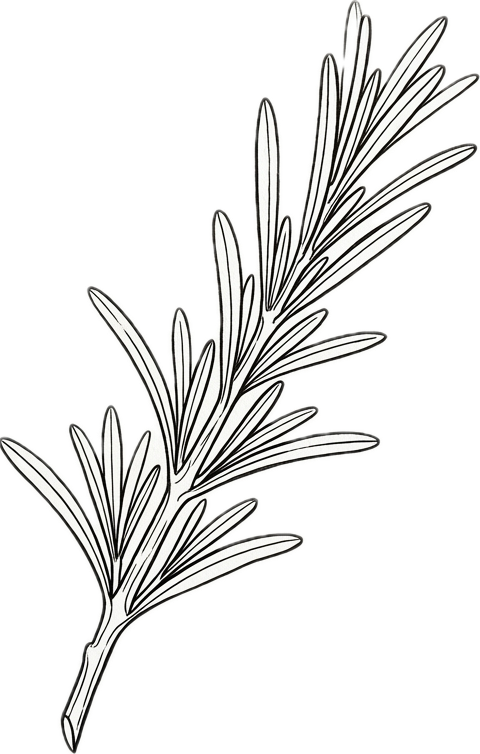
\includegraphics[width=1.5cm]{_extensions/nrennie/PrettyPDF/rosemary.png}
          }%
     }%
}

%% Style the page number
\fancypagestyle{mystyle}{
  \fancyhf{}
  \renewcommand\headrulewidth{0pt}
  \fancyfoot[R]{\thepage}
  \fancyfootoffset{3.5cm}
}
\setlength{\footskip}{20pt}

%% style the chapter/section fonts
\chapterfont{\color{dark}\fontsize{20}{16.8}\selectfont}
\sectionfont{\color{dark}\fontsize{20}{16.8}\selectfont}
\subsectionfont{\color{dark}\fontsize{14}{16.8}\selectfont}
\titleformat{\subsection}
  {\sffamily\Large\bfseries}{\thesection}{1em}{}[{\titlerule[0.8pt]}]
  
% left align title
\makeatletter
\renewcommand{\maketitle}{\bgroup\setlength{\parindent}{0pt}
\begin{flushleft}
  {\sffamily\huge\textbf{\MakeUppercase{\@title}}} \vspace{0.3cm} \newline
  {\Large {\@subtitle}} \newline
  \@author
\end{flushleft}\egroup
}
\makeatother

% Redefine \tableofcontents to not clear the page
\let\oldtableofcontents\tableofcontents
\renewcommand{\tableofcontents}{
  \begingroup
  \let\clearpage\relax
  \let\cleardoublepage\relax
  \oldtableofcontents
  \endgroup
}

%% Use some custom fonts
\setsansfont{Ubuntu}[
    Path=_extensions/nrennie/PrettyPDF/Ubuntu/,
    Scale=0.9,
    Extension = .ttf,
    UprightFont=*-Regular,
    BoldFont=*-Bold,
    ItalicFont=*-Italic,
    ]

\setmainfont{Ubuntu}[
    Path=_extensions/nrennie/PrettyPDF/Ubuntu/,
    Scale=0.9,
    Extension = .ttf,
    UprightFont=*-Regular,
    BoldFont=*-Bold,
    ItalicFont=*-Italic,
    ]
\KOMAoption{captions}{tableheading}
\makeatletter
\@ifpackageloaded{bookmark}{}{\usepackage{bookmark}}
\makeatother
\makeatletter
\@ifpackageloaded{caption}{}{\usepackage{caption}}
\AtBeginDocument{%
\ifdefined\contentsname
  \renewcommand*\contentsname{Table of contents}
\else
  \newcommand\contentsname{Table of contents}
\fi
\ifdefined\listfigurename
  \renewcommand*\listfigurename{List of Figures}
\else
  \newcommand\listfigurename{List of Figures}
\fi
\ifdefined\listtablename
  \renewcommand*\listtablename{List of Tables}
\else
  \newcommand\listtablename{List of Tables}
\fi
\ifdefined\figurename
  \renewcommand*\figurename{Figure}
\else
  \newcommand\figurename{Figure}
\fi
\ifdefined\tablename
  \renewcommand*\tablename{Table}
\else
  \newcommand\tablename{Table}
\fi
}
\@ifpackageloaded{float}{}{\usepackage{float}}
\floatstyle{ruled}
\@ifundefined{c@chapter}{\newfloat{codelisting}{h}{lop}}{\newfloat{codelisting}{h}{lop}[chapter]}
\floatname{codelisting}{Listing}
\newcommand*\listoflistings{\listof{codelisting}{List of Listings}}
\makeatother
\makeatletter
\makeatother
\makeatletter
\@ifpackageloaded{caption}{}{\usepackage{caption}}
\@ifpackageloaded{subcaption}{}{\usepackage{subcaption}}
\makeatother
\makeatletter
\@ifpackageloaded{tcolorbox}{}{\usepackage[skins,breakable]{tcolorbox}}
\makeatother
\makeatletter
\@ifundefined{shadecolor}{\definecolor{shadecolor}{rgb}{.97, .97, .97}}{}
\makeatother
\makeatletter
\@ifundefined{codebgcolor}{\definecolor{codebgcolor}{named}{light}}{}
\makeatother
\makeatletter
\ifdefined\Shaded\renewenvironment{Shaded}{\begin{tcolorbox}[frame hidden, colback={codebgcolor}, enhanced, boxrule=0pt, breakable, sharp corners]}{\end{tcolorbox}}\fi
\makeatother
\ifLuaTeX
  \usepackage{selnolig}  % disable illegal ligatures
\fi
\usepackage{bookmark}

\IfFileExists{xurl.sty}{\usepackage{xurl}}{} % add URL line breaks if available
\urlstyle{same} % disable monospaced font for URLs
\hypersetup{
  pdftitle={Slater Family Cookbook},
  pdfauthor={by Carson and Chloe Slater},
  colorlinks=true,
  linkcolor={highlight},
  filecolor={Maroon},
  citecolor={Blue},
  urlcolor={highlight},
  pdfcreator={LaTeX via pandoc}}

\title{Slater Family Cookbook}
\author{by Carson and Chloe Slater}
\date{2026-02-03}

\begin{document}
\maketitle

\pagestyle{mystyle}

\renewcommand*\contentsname{Table of contents}
{
\hypersetup{linkcolor=}
\setcounter{tocdepth}{2}
\tableofcontents
}
\bookmarksetup{startatroot}

\chapter{A Liturgy for Feasting with
Friends}\label{a-liturgy-for-feasting-with-friends}

\textbf{Leader:} To gather joyfully is indeed a serious affair, for
feasting and all enjoyments gratefully taken are, at their heart, acts
of war.

\textbf{People:} In celebrating this feast we declare that evil and
death, suffering and loss, sorrow and tears, will not have the final
word. But the joy of fellowship, and the welcome and comfort of friends
new and old, and the celebration of these blessings of food and drink
and conversation and laughter are the true evidences of things eternal,
and are the first fruits of that great glad joy that is to come and that
will be unending.

So let our feast this day be joined to those sure victories secured by
Christ. Let it be to us now a delight, and a glad foretaste of his
eternal kingdom. Bless us, O Lord, in this feast.

Bless us, O Lord, as we linger over our cups, And over tables laden with
good things, as we relish the delights of varied texture and flavor, Of
aromas and savory spices, Of dishes prepared as acts of love and
blessing, Of sweet delights made sweeter by the communion of saints.

May this shared meal, and our pleasure in it, bear witness against the
artifice and deceptions of the prince of the darkness that would blind
this world to hope. May it strike at the root of the lie that would
drain life of meaning, and the world of joy, and suffering of
redemption. May this our feast fall like a great hammer blow against
that brittle night, Shattering the gloom, reawakening our hearts,
stirring our imaginations, focusing our vision On the kingdom of heaven
that is to come On the kingdom that is promised On the kingdom that is
already, indeed, among us, For the resurrection of all good things has
already joyfully begun.

May this feast be an echo of that great supper of the Lamb, and a
foreshadowing of the great celebration that awaits the children of God.

Where two or more of us are gathered, O Lord, there you have promised to
be And here we are And so, here are you. Take joy, O King, in this our
feast. Take joy, O King!

\textbf{Leader:} All will be well!

\textbf{People:} All will be well! Nothing good and right and true will
be lost forever. All good things will be restored. Feast and be
reminded! Take joy, little flock. Take joy! Let battle be joined! Let
battle be joined!

Now you who are loved by the Father, prepare your hearts and give
yourselves wholly to this celebration of joy, to the glad company of
saints, to the comforting fellowship of the Spirit, and to the abiding
presence of Christ who is seated among us both as our host and as our
honored guest, and still yet as our conquering king. Amen.

In the name of the Father, the Son, and the Holy Spirit, take seat, take
feast, take delight!

\emph{Copyright 2016 by Douglas Kaine McKelvey}

\bookmarksetup{startatroot}

\chapter{Chicken Posole Verde}\label{chicken-posole-verde}

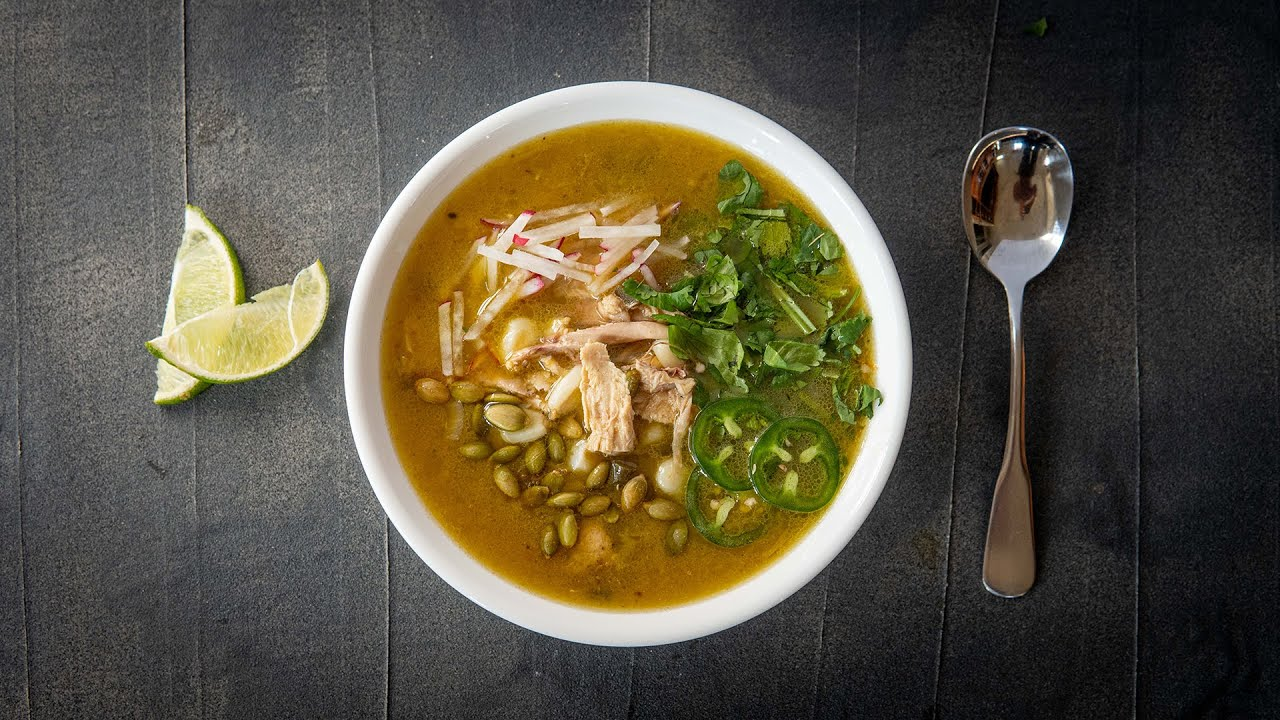
\includegraphics[width=1\textwidth,height=\textheight]{images/chicken-posole-verde.jpg}

\textbf{Prep Time:} \textbar{} \textbf{Cook Time:} \textbar{}
\textbf{Total Time:} 1 hr 30 min

\section{Ingredients}\label{ingredients}

\begin{itemize}
\tightlist
\item
  Tomatillos, 12-15
\item
  Poblano peppers, 3-4
\item
  Ghost pepper, 1
\item
  Serrano peppers, 2
\item
  Yellow onion, 1
\item
  Garlic, 6 cloves
\item
  Whole Chicken, 1
\item
  chicken stock, 1800 g
\item
  hominy, 850 g
\item
  Cumin, 3 g
\item
  Ground coriander, 2 g
\item
  Chili Powder, 2 g
\item
  Salt,
\item
  Black Pepper,
\item
  Pickled onions,
\item
  Jalapeños,
\item
  Crema,
\item
  Radishes, thinly sliced
\item
  Cilantro,
\item
  Cotija cheese,
\item
  Limes,
\item
  Pepitas,
\end{itemize}

\section{Instructions}\label{instructions}

\begin{itemize}
\tightlist
\item
  Turn the oven on broil at 500° F/260° C.
\item
  Spread tomatillos, poblano and serrano peppers on a large tin foil
  rimmed baking sheet. Broil for 5 minutes until blackened and charred.
  Let cool 10 minutes.
\item
  Meanwhile, finely chop the yellow onion and garlic cloves. Add them to
  a bowl.
\item
  Once cooled, finely chop the roasted tomatillos, poblanos, and serrano
  peppers and add them to the bowl.
\item
  Cut the whole chicken into 10 pieces.
\item
  If you haven't broken down a chicken yet, check out the video for how
  I do this.
\item
  Next, heat a thin layer of vegetable oil in a large Dutch oven over
  medium-high heat.
\item
  Liberally season the chicken pieces with salt and pepper.
\item
  Add them to the Dutch oven to sear and brown on all sides. Set the
  browned chicken pieces on a plate and turn the heat to medium-low.
\item
  To the same pot that the chicken was browned in, add the bowl of
  chopped vegetables, ground spices, and a pinch of salt to the pot.
  Sauté, stirring occasionally, for 10-15 minutes.
\item
  Set the heat to low and sauté for another 15-20 minutes until
  everything is caramelized and reduced.
\item
  Pour in the chicken stock and deglaze the pot.
\item
  Add the browned chicken pieces. Bring the soup to a simmer and cook,
  uncovered, for 20-30 minutes.
\item
  Remove the chicken pieces and shred them, picking out any bones or
  inedible pieces. Return the shredded chicken to the soup and add the
  hominy.
\item
  Taste it and add salt and pepper as needed.
\item
  Serve in bowls and top with pickled red onion, sliced jalapeño, crema,
  radish, cilantro, cotija, fresh squeezed lime, or any other desired
  toppings.
\end{itemize}

\bookmarksetup{startatroot}

\chapter{Thai Pizza}\label{thai-pizza}

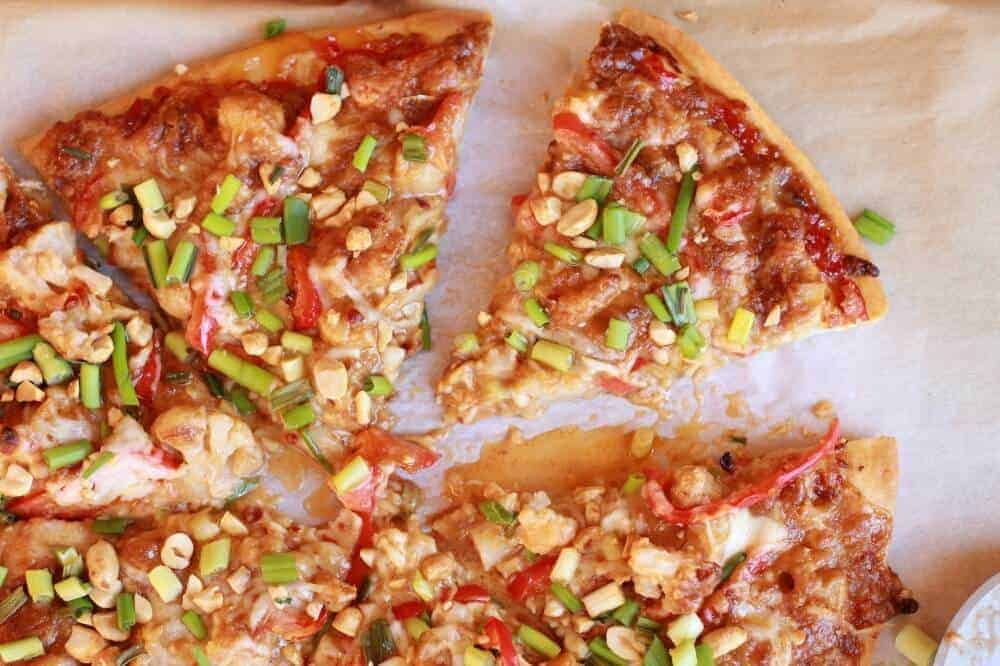
\includegraphics[width=1\textwidth,height=\textheight]{images/thai-pizza.jpg}

\textbf{Prep Time:} 2 hr \textbar{} \textbf{Cook Time:} 35 min
\textbar{} \textbf{Total Time:} 2 hr 35 min

\section{Ingredients}\label{ingredients-1}

\begin{itemize}
\tightlist
\item
  1 cup warm water (100-105 degrees)
\item
  2 1/4 teaspoons active dry yeast
\item
  2 tablespoons honey (divided)
\item
  2 tablespoon olive oil
\item
  3 cups all-purpose flour
\item
  1 1/2 teaspoons kosher salt
\item
  1/2- 1 cups sweet red chili sauce
\item
  1 cup mozzarella cheese (shredded, plus more for sprinkling)
\item
  1/2 cup peanut butter
\item
  5 tablespoons coconut milk
\item
  3 tablespoons soy sauce
\item
  1 tablespoon fish sauce
\item
  3 teaspoon sambal oelek
\item
  1 tablespoon honey
\item
  1 teaspoon chili oil
\item
  1 tablespoons ginger (freshly minced)
\item
  2 cloves garlic (minced)
\item
  1 small head cauliflower (chopped into bit size pieces)
\item
  2 red bell peppers (julienned)
\item
  4 green onions (sliced, for garnish)
\item
  chopped peanuts (for garnish)
\end{itemize}

\section{Instructions}\label{instructions-1}

\begin{enumerate}
\def\labelenumi{\arabic{enumi}.}
\tightlist
\item
  For the Dough: In a large bowl, combine water, yeast and honey. Mix
  with a spoon, then let sit until foamy, about 10 minutes. Add in 2 1/2
  cups flour and olive oil stirring with a spoon until the dough comes
  together but is still sticky. Using your hands, form the dough into a
  ball and work the additional 1/2 cup flour in to the dough, kneading
  it on a floured surface for a few minutes. You can also do all the
  mixing and kneading in your stand mixer with the dough hook
  attachment. Rub the same bowl with olive oil then place the dough
  inside, turning to coat. Cover with a towel and place in a warm place
  to rise for about 1 1/2 hours.
\item
  To make the Pizza's: Preheat the oven to 375 degrees.
\item
  Once the pizza dough is ready to go dived the dough in half. Place
  half the dough aside for another use or freeze for later. With the
  remaining dough roll/press into two medium size round pizzas (I like
  to divide my dough in half (again) and make two medium pizza's rather
  than one large. I find the the pizzas cook better at a smaller size.).
  They do not have to be perfect! Roll the dough as thin as possible or
  until you reach your desired thickness.
\item
  Spread the sweet asian chili sauce all over the pizza dough leaving
  about a half inch border for the crust. Add the mozzarella cheese.
\item
  In a large bowl, whisk together the peanut butter through the garlic.
  Toss the cauliflower in the peanut sauce. Using a fork remove the
  cauliflower and distribute evenly atop the pizzas. Reserve any
  remaining sauce for drizzling.
\item
  Scatter the red peppers on top and drizzle with any remaining peanut
  sauce. If desired sprinkle with a handful more of mozzarella cheese.
\item
  Bake at 375 degrees for 30- 35 minutes or until your desired doneness.
  Sprinkle with green onions and chopped peanuts.
\item
  Let sit for 5 mintes before cutting.
\end{enumerate}

\bookmarksetup{startatroot}

\chapter{Bourbon Pecan Cherry Hand
Pies}\label{bourbon-pecan-cherry-hand-pies}

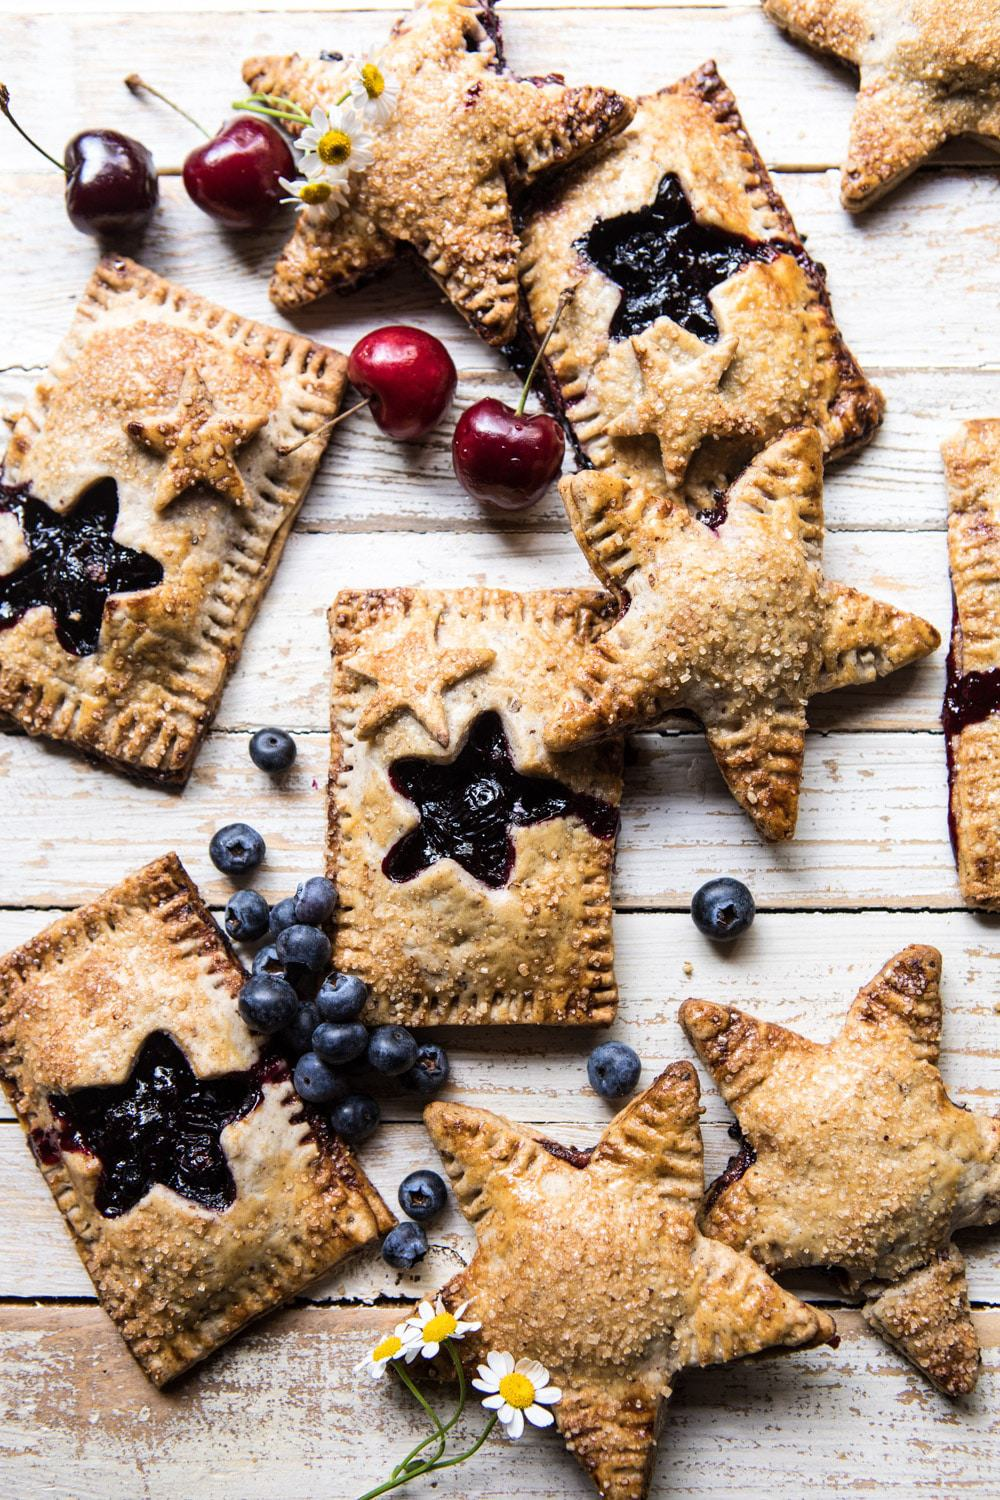
\includegraphics[width=1\textwidth,height=\textheight]{images/bourbon-pecan-cherry-hand-pies.jpg}

\textbf{Prep Time:} 30 min \textbar{} \textbf{Cook Time:} 30 min
\textbar{} \textbf{Total Time:} 1 hr

\section{Ingredients}\label{ingredients-2}

\begin{itemize}
\tightlist
\item
  3-4 cups fresh cherries, pitted
\item
  1/2 cup granulated sugar
\item
  2 teaspoons lemon juice
\item
  1 cup fresh blueberries
\item
  1-2 tablespoons bourbon
\item
  2 1/2 cups all-purpose flour, plus more for rolling
\item
  3/4 cup finely ground toasted pecans
\item
  1 cup (2 sticks) chilled salted butter, cut into pieces
\item
  1/3 cup ice water, plus more if needed
\item
  1 whole egg, beaten
\item
  coarse sugar, for sprinkling
\end{itemize}

\section{Instructions}\label{instructions-2}

\begin{enumerate}
\def\labelenumi{\arabic{enumi}.}
\tightlist
\item
  In a medium saucepan, bring the cherries, sugar, lemon juice, and 2
  tablespoons water to a boil over high heat. Once boiling use a potato
  masher or fork to break down and mash the cherries. Continue to cook
  for 8-10 minutes or until the jam has reduced and thickened by 1/3.
  Stir in the blueberries and cook another 5 minutes.
\item
  Remove from the heat and stir in the bourbon. Let cool completely
  before filling.
\item
  To make the crust. Add the flour pecans and butter to a food processor
  and pulse until the mixture is combined and resembles peas. Add the
  ice water and mix with a wooden spoon, drizzling in more water as
  needed (no more than 1 tablespoon at a time), until dough just comes
  together (a few dry spots are ok).
\item
  Divide the dough in half. Shape each piece into a circular disk. At
  this point you can cover the dough and place it in the fridge for up
  to one week OR continue on with the recipe\ldots yes, no chilling
  needed!
\item
  Roll the dough out into a 1/8-inch thickness. Cut the dough into
  rectangles, about 6 1/2 x 4 1/2 inches. If desired, use a small star
  cookie cutter to cut stars out of half of the rectangles (see above
  photo).
\item
  Place a tablespoon of jam on one half of the rectangle. Lay the other
  half of the dough over the filling and seal the edges by crimping with
  the back of a fork. Repeat until you have used all the dough, you may
  have leftover jam. Place the pies on parchment lined baking sheets.
  Cover the baking sheets and place in the freezer for 20-30 minutes to
  chill.
\item
  Preheat the oven to 375 degrees F. Brush the pies with the beaten egg
  and sprinkle with the coarse sugar. Bake 15-20 minutes or until golden
  in color. Serve warm or at room temperature.
\end{enumerate}

\bookmarksetup{startatroot}

\chapter{Toasted S'more Chocolate Ice Cream
Cups}\label{toasted-smore-chocolate-ice-cream-cups}

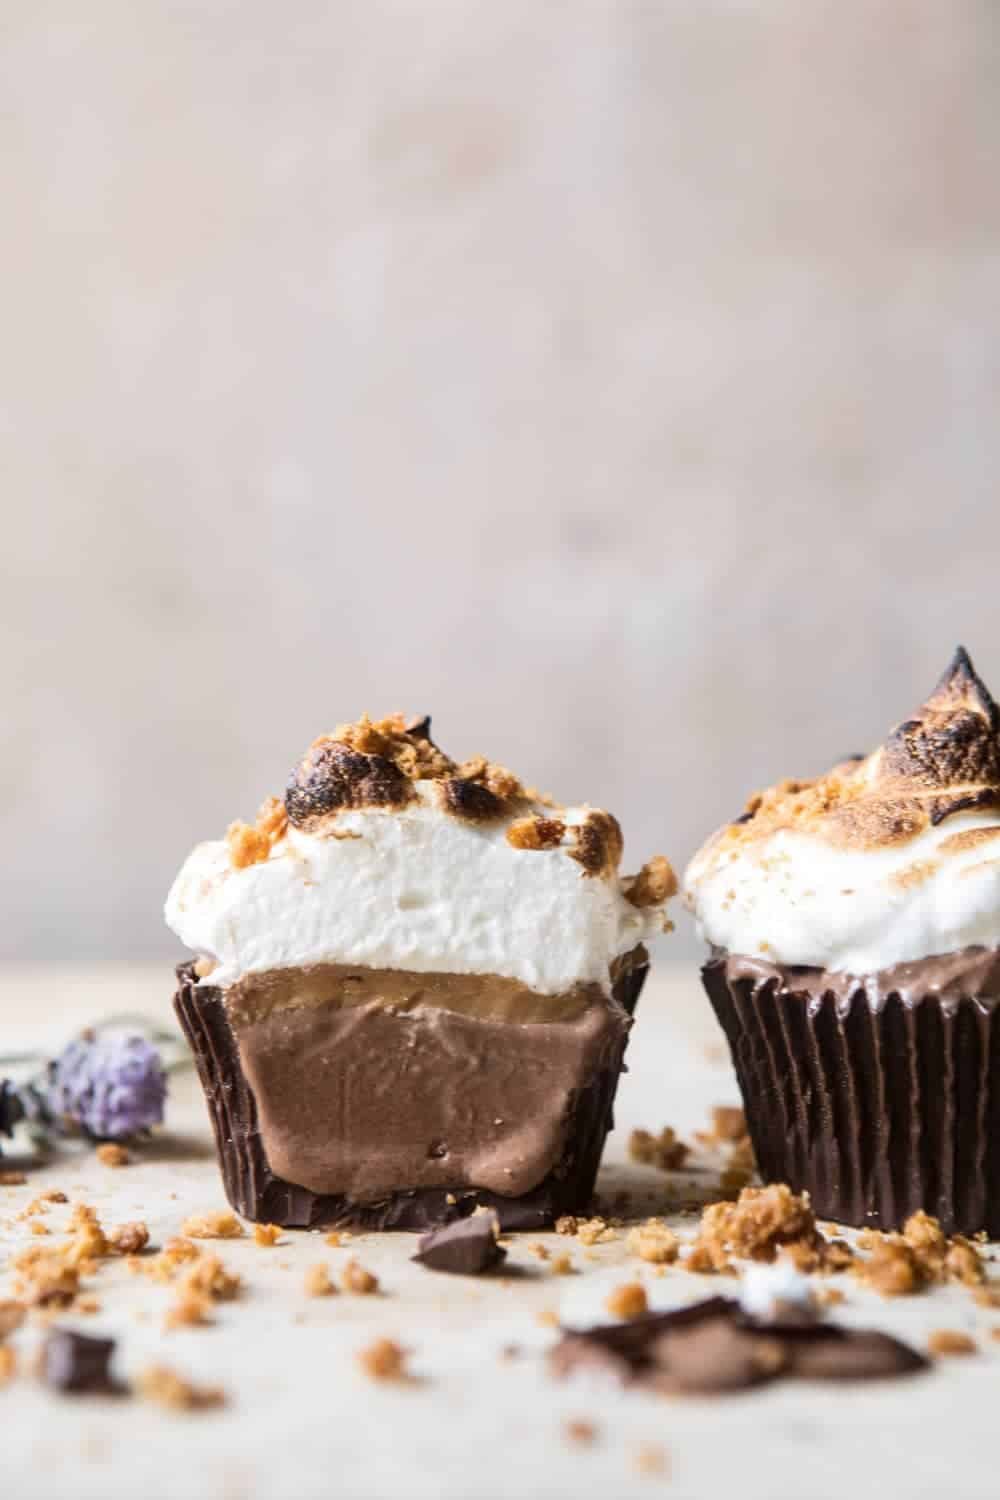
\includegraphics[width=1\textwidth,height=\textheight]{images/toasted-s-more-chocolate-ice-cream-cups.jpg}

\textbf{Prep Time:} 30 min \textbar{} \textbf{Cook Time:} 5 min
\textbar{} \textbf{Total Time:} 35 min

\section{Ingredients}\label{ingredients-3}

\begin{itemize}
\tightlist
\item
  1 sleeve of graham crackers, crushed
\item
  6 tablespoons salted butter, softened
\item
  1 tablespoon honey
\item
  12 ounces semi-sweet chocolate, melted
\item
  6 cups chocolate ice cream
\item
  1/2 cup creamy peanut butter ((optional))
\item
  4 large egg whites
\item
  1 cup granulated or caster (powdered) sugar
\item
  1/2 teaspoon vanilla extract
\end{itemize}

\section{Instructions}\label{instructions-3}

\begin{enumerate}
\def\labelenumi{\arabic{enumi}.}
\tightlist
\item
  Preheat an oven to 325 degrees F. Line a baking sheet with parchment
  paper.
\item
  To make the graham cracker crumble. Combine the graham crackers,
  butter, and honey in a medium bowl. Transfer to the prepared baking
  sheet and bake until light golden brown, about 10 minutes.
\item
  Place 12 cupcake liners in a cupcake mold. Using the back of a spoon,
  smooth the melted chocolate up the sides of the liners. Sprinkle a
  little of the graham cracker crumble into the bottom of each cup
  (reserve the rest for serving). Place in the freezer for 10-15 minutes
  or until firm. Fill each cup with chocolate ice cream and a layer of
  peanut butter, if using. Freeze until firm, about 1-2 hours or
  overnight.
\item
  Just before serving, make the marshmallow. Bring a large pot of water
  to simmer. Whisk the egg whites and sugar together in the bowl of a
  stand mixer. Place the bowl of the stand mixer over the pot of
  simmering water and cook, stirring often, until the egg whites are
  very warm to the touch and the sugar has dissolved, remove the bowl
  from the heat. Whip the egg whites on high until stiff peaks form. Add
  the vanilla and whip to combine.
\item
  Top the frozen cups with marshmallow. Using a blow torch, toast the
  marshmallow. Serve immediately.
\end{enumerate}

\bookmarksetup{startatroot}

\chapter{Honey Strawberry Muffins}\label{honey-strawberry-muffins}

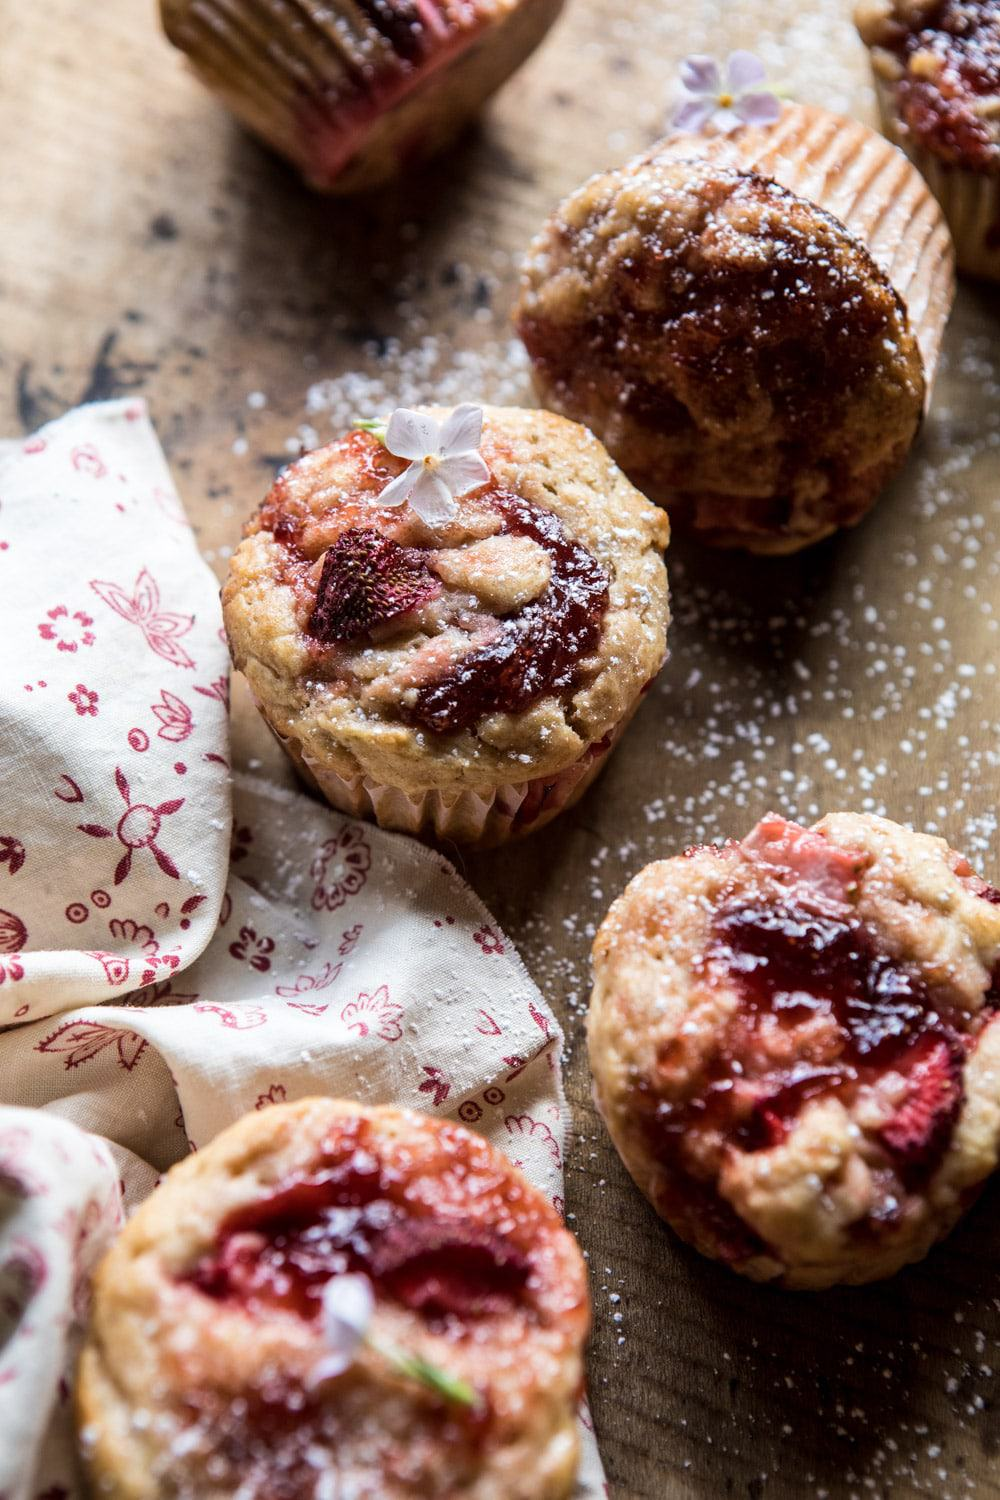
\includegraphics[width=1\textwidth,height=\textheight]{images/honey-strawberry-muffins.jpg}

\textbf{Prep Time:} 10 min \textbar{} \textbf{Cook Time:} 20 min
\textbar{} \textbf{Total Time:} 30 min

\section{Ingredients}\label{ingredients-4}

\begin{itemize}
\tightlist
\item
  1/2 cup salted butter, melted
\item
  1/2 cup runny honey
\item
  2 teaspoons vanilla extract
\item
  1 cup whole milk or buttermilk
\item
  1/2 cup plain greek yogurt
\item
  2 eggs
\item
  1 1/2 cups all-purpose flour
\item
  1 cup whole wheat flour
\item
  2 teaspoons baking powder
\item
  1/2 teaspoon baking soda
\item
  1 cup fresh strawberries, diced
\item
  1/2 cup high quality strawberry jam
\item
  2 teaspoons lemon zest
\end{itemize}

\section{Instructions}\label{instructions-4}

\begin{enumerate}
\def\labelenumi{\arabic{enumi}.}
\tightlist
\item
  Preheat the oven to 350 degrees F. Lightly coat 18 muffin tins with
  nonstick spray.
\item
  In a large mixing bowl, whisk together the melted butter, honey,
  vanilla, buttermilk, greek yogurt, and eggs until smooth. Add the
  flour, whole wheat flour, baking powder, and baking soda, and mix
  until just combined.
\item
  In a small bowl, stir together the strawberries, jam, and lemon zest.
  Gently fold the berries into the batter, being careful not to over
  mix, you are going for a swirled look.
\item
  Divide the batter evenly among the prepared muffins tins. Transfer to
  the oven and bake for 25-30 minutes or until a toothpick inserted into
  the center comes out clean.
\item
  Serve the muffins warm or at room temp with a smear of butter. Enjoy!
\end{enumerate}

\bookmarksetup{startatroot}

\chapter{Creamy Mocha Custard}\label{creamy-mocha-custard}

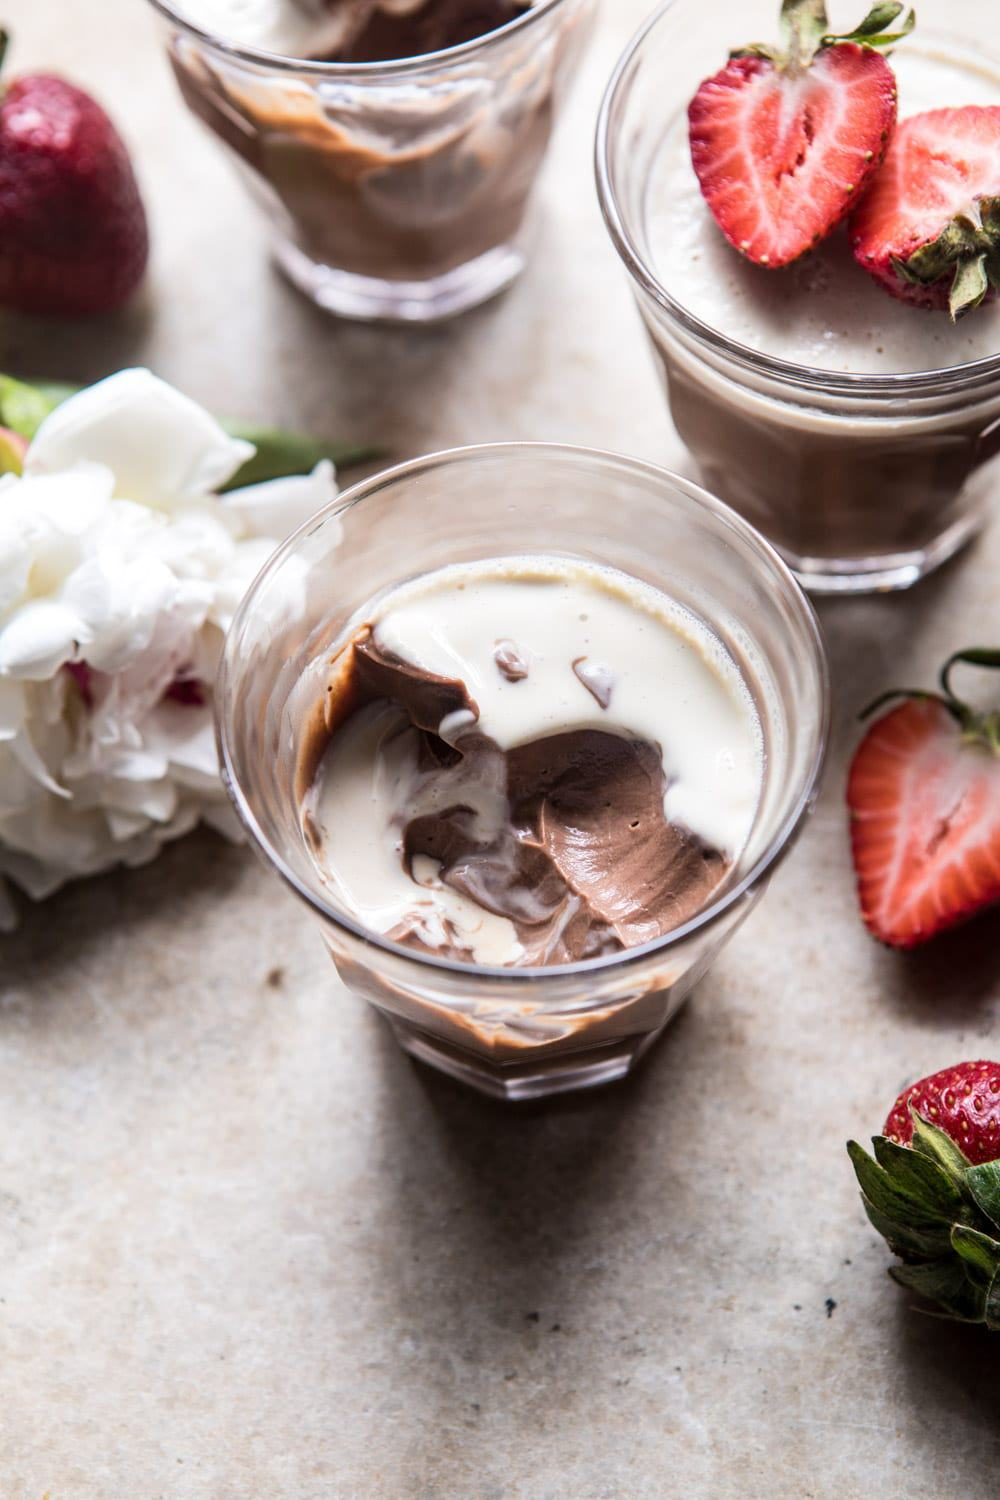
\includegraphics[width=1\textwidth,height=\textheight]{images/creamy-mocha-custard.jpg}

\textbf{Prep Time:} 10 min \textbar{} \textbf{Cook Time:} 10 min
\textbar{} \textbf{Total Time:} 20 min

\section{Ingredients}\label{ingredients-5}

\begin{itemize}
\tightlist
\item
  3 egg yolks
\item
  1/2 cup honey
\item
  3 1/2 cups heavy cream
\item
  pinch of sea salt
\item
  1/4 cup brewed black coffee
\item
  1 tablespoon vanilla extract
\item
  10 ounces semi-sweet or dark chocolate, chopped
\end{itemize}

\section{Instructions}\label{instructions-5}

\begin{enumerate}
\def\labelenumi{\arabic{enumi}.}
\tightlist
\item
  In a large pot, whisk together the egg yolks and honey. Add the cream
  and sea salt. Set the pot over medium-high heat and bring the mixture
  to a boil. Cook, stirring continuously, until the mixture thickens and
  easily coats the back of a wooden spoon, 5-8 minutes. Watch close,
  milk tends to boil over. Remove from the heat. Stir in the coffee and
  vanilla.
\item
  Remove 3/4 cup of the vanilla custard and set aside.
\item
  Add the chocolate to the remaining custard and stir until melted and
  smooth.
\item
  Divide the chocolate custard among six glasses. Freeze 1 hour and then
  evenly pour over the reserved vanilla custard. Freeze until set, about
  2 hours. Keep in the fridge or freezer. If frozen, let sit at room
  temp for 10 minutes before serving. If kept in the fridge the vanilla
  custard will be runny.
\end{enumerate}

\bookmarksetup{startatroot}

\chapter{Skillet Lemon Pepper Chicken and Garden
Veggies}\label{skillet-lemon-pepper-chicken-and-garden-veggies}

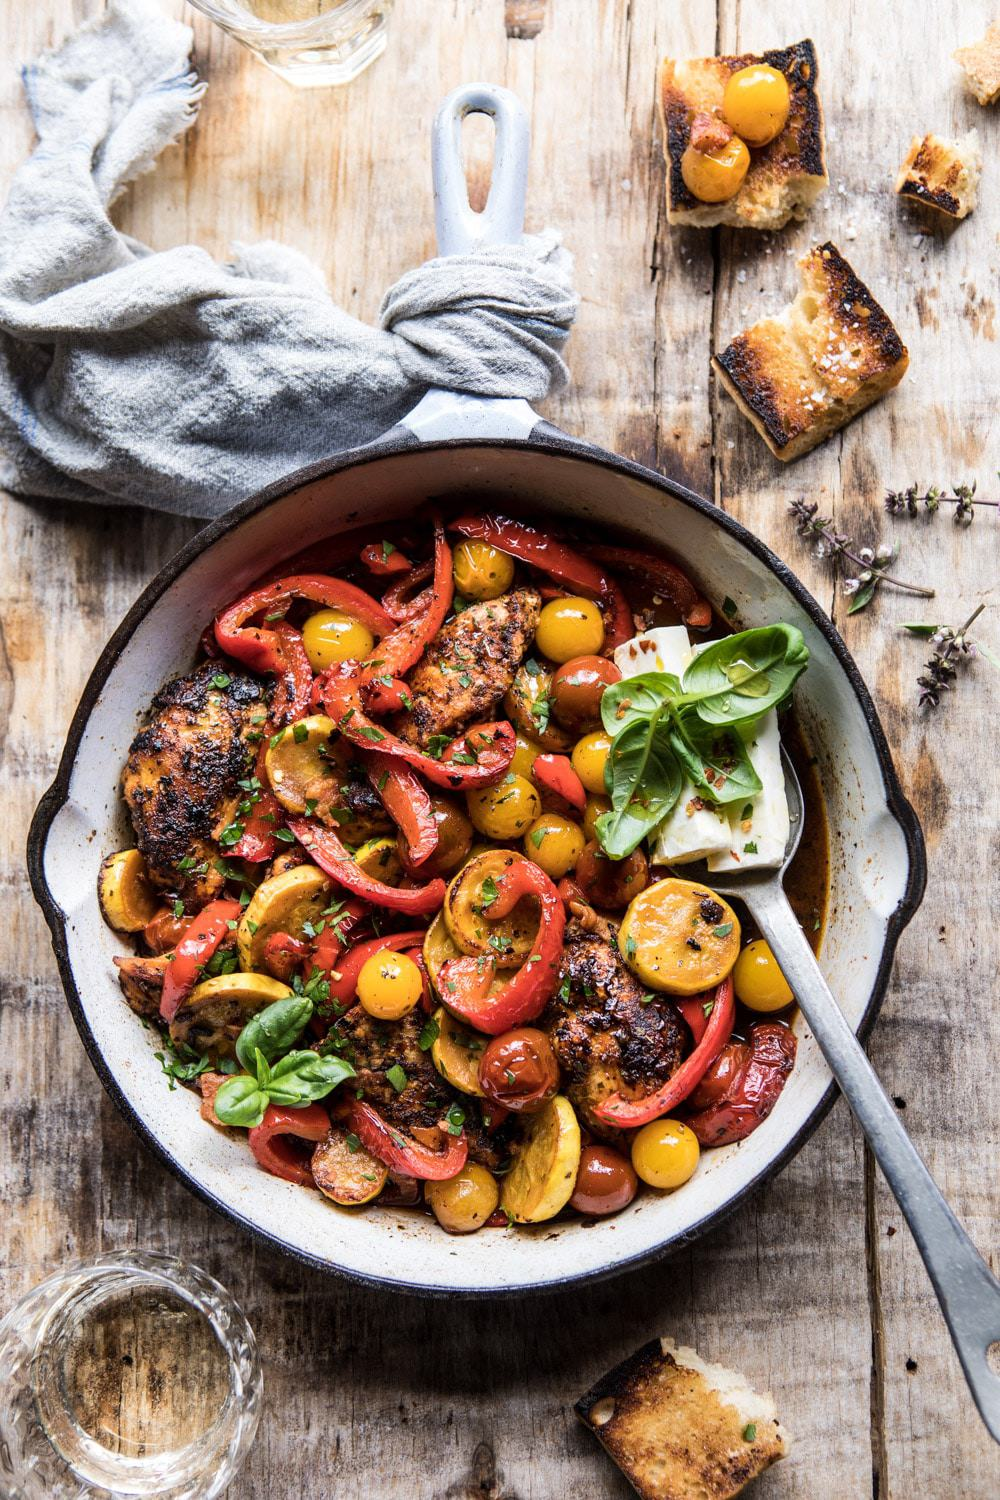
\includegraphics[width=1\textwidth,height=\textheight]{images/skillet-lemon-pepper-chicken-and-garden-veggies.jpg}

\textbf{Prep Time:} 10 min \textbar{} \textbf{Cook Time:} 20 min
\textbar{} \textbf{Total Time:} 30 min

\section{Ingredients}\label{ingredients-6}

\begin{itemize}
\tightlist
\item
  1 pound boneless skinless chicken breasts
\item
  1/4 cup extra virgin olive oil
\item
  4 cloves garlic, minced or grated
\item
  2 teaspoons smoked paprika
\item
  1 teaspoon onion powder
\item
  1/2 teaspoon cayenne
\item
  1/4 cup fresh parsley, chopped
\item
  1/4 cup fresh basil, chopped
\item
  zest and juice of 1 lemon
\item
  kosher salt and pepper
\item
  2 red bell peppers, sliced
\item
  1 zucchini or yellow summer squash, chopped
\item
  1 cup cherry tomatoes
\item
  3/4 cup white wine, Such as Pinot Grigio or Sauvignon Blanc
\item
  4 ounces feta cheese, cubed
\end{itemize}

\section{Instructions}\label{instructions-6}

\begin{enumerate}
\def\labelenumi{\arabic{enumi}.}
\tightlist
\item
  Toss the chicken with 2 tablespoons olive oil, garlic, paprika, onion
  powder, cayenne, parsley, basil, lemon juice, and lemon zest. Season
  generously with salt and pepper.
\item
  Add the remaining 2 tablespoons olive oil and chicken to the pan and
  sear on both sides until golden, about 5 minutes per side. Add the
  peppers and zucchini and cook another 5 minutes. Next add the
  tomatoes, shake the pan and cook for 1 minute. Reduce the heat to
  medium low and pour in the wine. Simmer the chicken for 10-15 minutes
  until cooked through.
\item
  Serve the chicken topped with feta. Drizzle any remaining pan sauce
  overtop, and top with basil. EAT!
\end{enumerate}

\bookmarksetup{startatroot}

\chapter{Chocolate Dipped Peanut Cookie Ice Cream
Sandwiches}\label{chocolate-dipped-peanut-cookie-ice-cream-sandwiches}

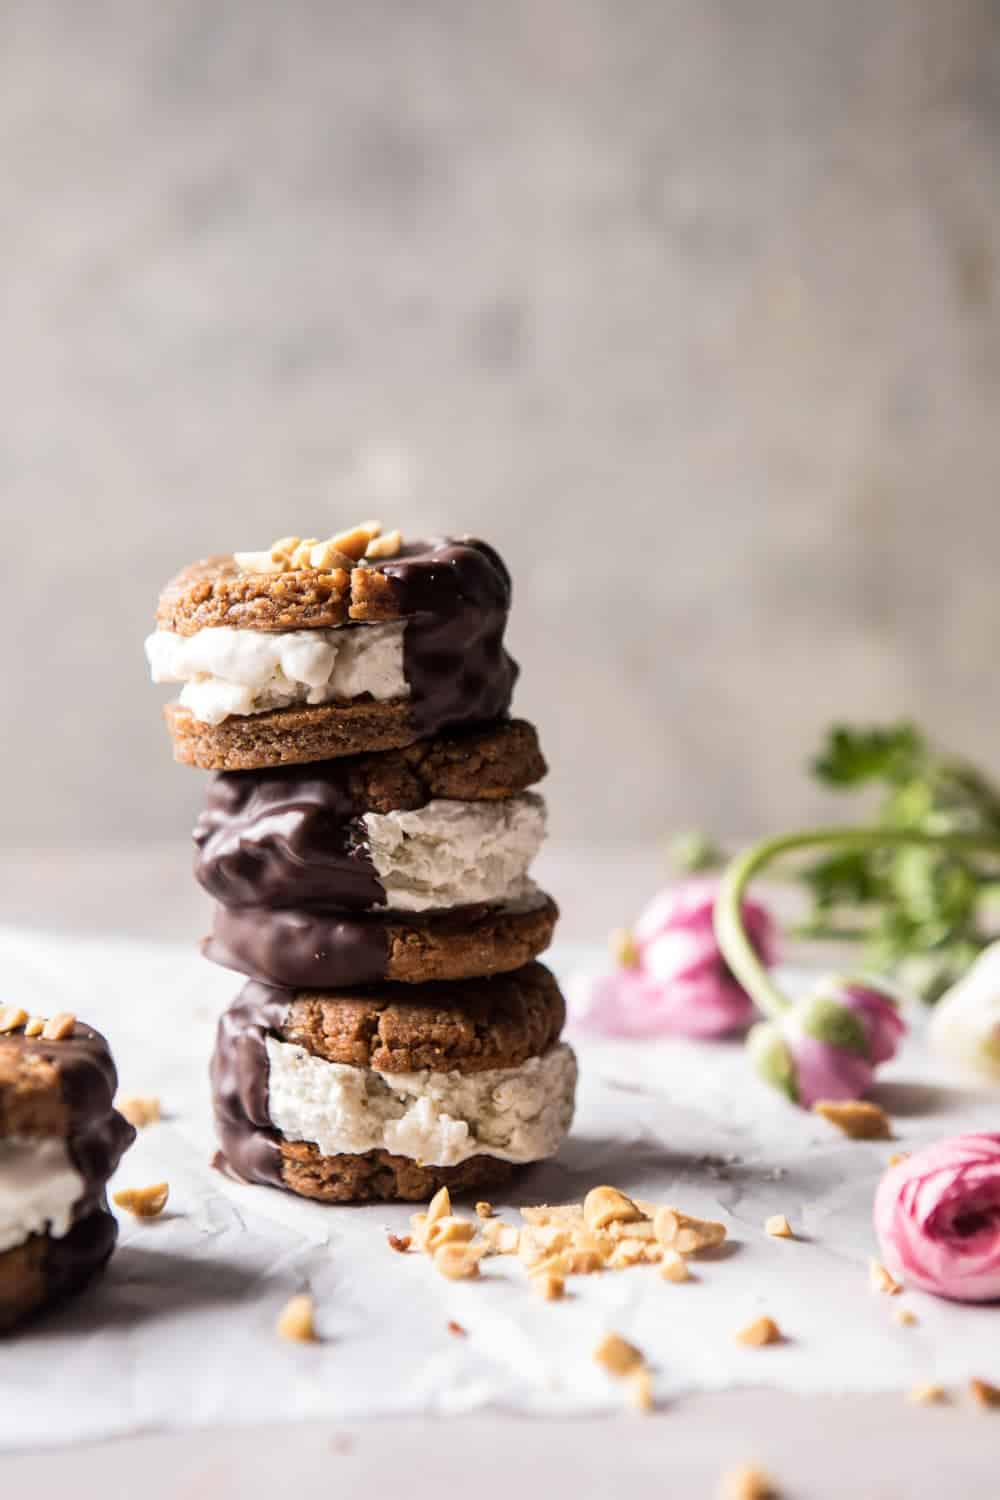
\includegraphics[width=1\textwidth,height=\textheight]{images/chocolate-dipped-peanut-cookie-ice-cream-sandwiches.jpg}

\textbf{Prep Time:} 20 min \textbar{} \textbf{Cook Time:} 10 min
\textbar{} \textbf{Total Time:} 30 min

\section{Ingredients}\label{ingredients-7}

\begin{itemize}
\tightlist
\item
  1 cup creamy peanut butter or almond butter
\item
  8 ounces pitted medjool dates (1 cup packed dates)
\item
  2 teaspoons vanilla extract
\item
  1 egg
\item
  vanilla or chocolate ice cream or frozen yogurt
\item
  8 ounces melted dark chocolate
\item
  1 tablespoon coconut oil
\end{itemize}

\section{Instructions}\label{instructions-7}

\begin{enumerate}
\def\labelenumi{\arabic{enumi}.}
\tightlist
\item
  Preheat the oven to 350 degrees F. Line a baking sheet with parchment
  paper.
\item
  In the bowl of a food processor, combine the peanut butter, dates, and
  vanilla. Pulse until well combined and no large chunks of dates
  remain. Add the egg and pulse to combine. Roll the dough into 16 balls
  and place on the prepared baking sheet. Using a fork, gently press
  down on each dough ball to flatten and create a cross hatch pattern.
  Transfer to the oven and bake for 9-10 minutes. It's important not to
  over bake these cookies, so set a timer!
\item
  Remove the cookies from the oven and let cool. Using an ice cream
  scoop, scoop 1 scoop of ice cream on to half of the cookies. Sandwich
  with the remaining cookies, gently pushing down. Transfer to the
  freezer and freeze for 15 minutes.
\item
  Meanwhile, melt together the chocolate and coconut oil in a microwave
  safe bowl.
\item
  Drizzle or dip the sandwiches in chocolate. The chocolate should begin
  to harden. Eat and enjoy or return to the freezer. Remove from freezer
  5-10 minutes before eating.
\end{enumerate}

\bookmarksetup{startatroot}

\chapter{Chocolate Peanut Butter Honey Cheerio
Bars}\label{chocolate-peanut-butter-honey-cheerio-bars}

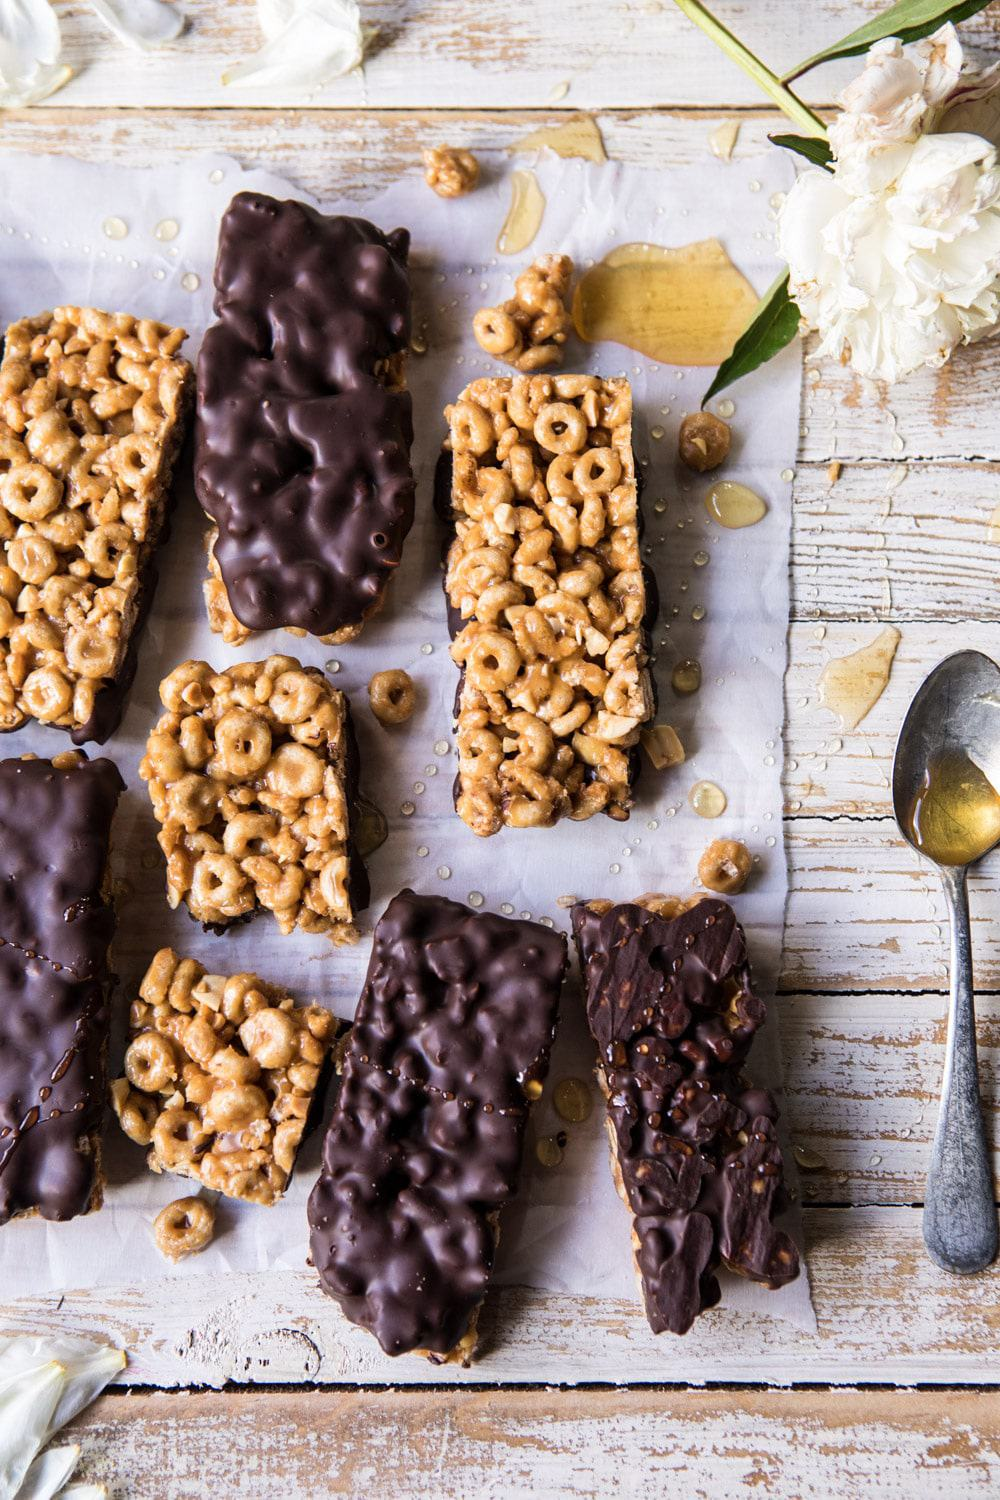
\includegraphics[width=1\textwidth,height=\textheight]{images/chocolate-peanut-butter-honey-cheerio-bars.jpg}

\textbf{Prep Time:} 15 min \textbar{} \textbf{Cook Time:} \textbar{}
\textbf{Total Time:} 15 min

\section{Ingredients}\label{ingredients-8}

\begin{itemize}
\tightlist
\item
  1/2 cup honey
\item
  1/2 cup creamy peanut butter
\item
  3 cups Cheerios cereal
\item
  1 cup Brown Rice Krispies
\item
  1/2 cup roasted peanuts, chopped
\item
  8-12 ounces semi-sweet or dark chocolate, melted
\end{itemize}

\section{Instructions}\label{instructions-8}

\begin{enumerate}
\def\labelenumi{\arabic{enumi}.}
\tightlist
\item
  Line a 9x13 inch baking pan with parchment paper.
\item
  In a large, microwave safe bowl, melt together the honey and peanut
  butter until smooth, about 30 second to 1 minute. Stir in the
  Cheerios, Brown Rice Krispies, and peanuts, tossing well to combine.
  Spread the mix out into the prepared pan, packing it in tightly.
  Transfer to the freezer and freeze 15-20 minutes.
\item
  Remove the pan from the freezer and cut into 16 bars. Working quickly,
  dip each bar in chocolate and place on a parchment lined baking sheet.
  Return to the freezer for 10 minutes. Keep stored in the fridge or
  freezer.
\end{enumerate}

\bookmarksetup{startatroot}

\chapter{Chocolate Coconut Latte Fudge
Popsicles}\label{chocolate-coconut-latte-fudge-popsicles}


\includegraphics[width=1\textwidth,height=\textheight]{images/chocolate-coconut-latte-fudge-popsicles.jpg}

\textbf{Prep Time:} 20 min \textbar{} \textbf{Cook Time:} \textbar{}
\textbf{Total Time:} 6 hr 20 min

\section{Ingredients}\label{ingredients-9}

\begin{itemize}
\tightlist
\item
  1 cup raw cashews
\item
  1 1/2 cups full fat canned coconut milk
\item
  1/2 cup pitted medjool dates
\item
  2 teaspoons vanilla extract
\item
  1 pinch flaky sea salt
\item
  6 tablespoons brewed coffee
\item
  8 ounces dark chocolate, melted
\end{itemize}

\section{Instructions}\label{instructions-9}

\begin{enumerate}
\def\labelenumi{\arabic{enumi}.}
\tightlist
\item
  Bring a small pot of water to a boil. Add the cashews and let sit 15
  minutes or up to 2 hours. Drain.
\item
  In a high power blender or food processor, combine the cashews,
  coconut milk, dates, vanilla, pinch of salt and 2 tablespoons coffee.
  Blend until completely smooth and the consistency of a thick smoothie.
\item
  Evenly divide the remaining coffee among 7-8 popsicle molds. Spoon the
  cashew mix over the coffee, it should naturally create a swirl of
  coffee. Insert popsicle sticks, cover the tops of the mold, and freeze
  until firm, about 4 hours. To remove the popsicles run the mold under
  hot water for 10 seconds and then pull the popsicles out of the molds.
\item
  Dip each popsicle in chocolate. Store in the freezer.
\end{enumerate}

\bookmarksetup{startatroot}

\chapter{No Bake Greek Yogurt Fruit
Tart}\label{no-bake-greek-yogurt-fruit-tart}

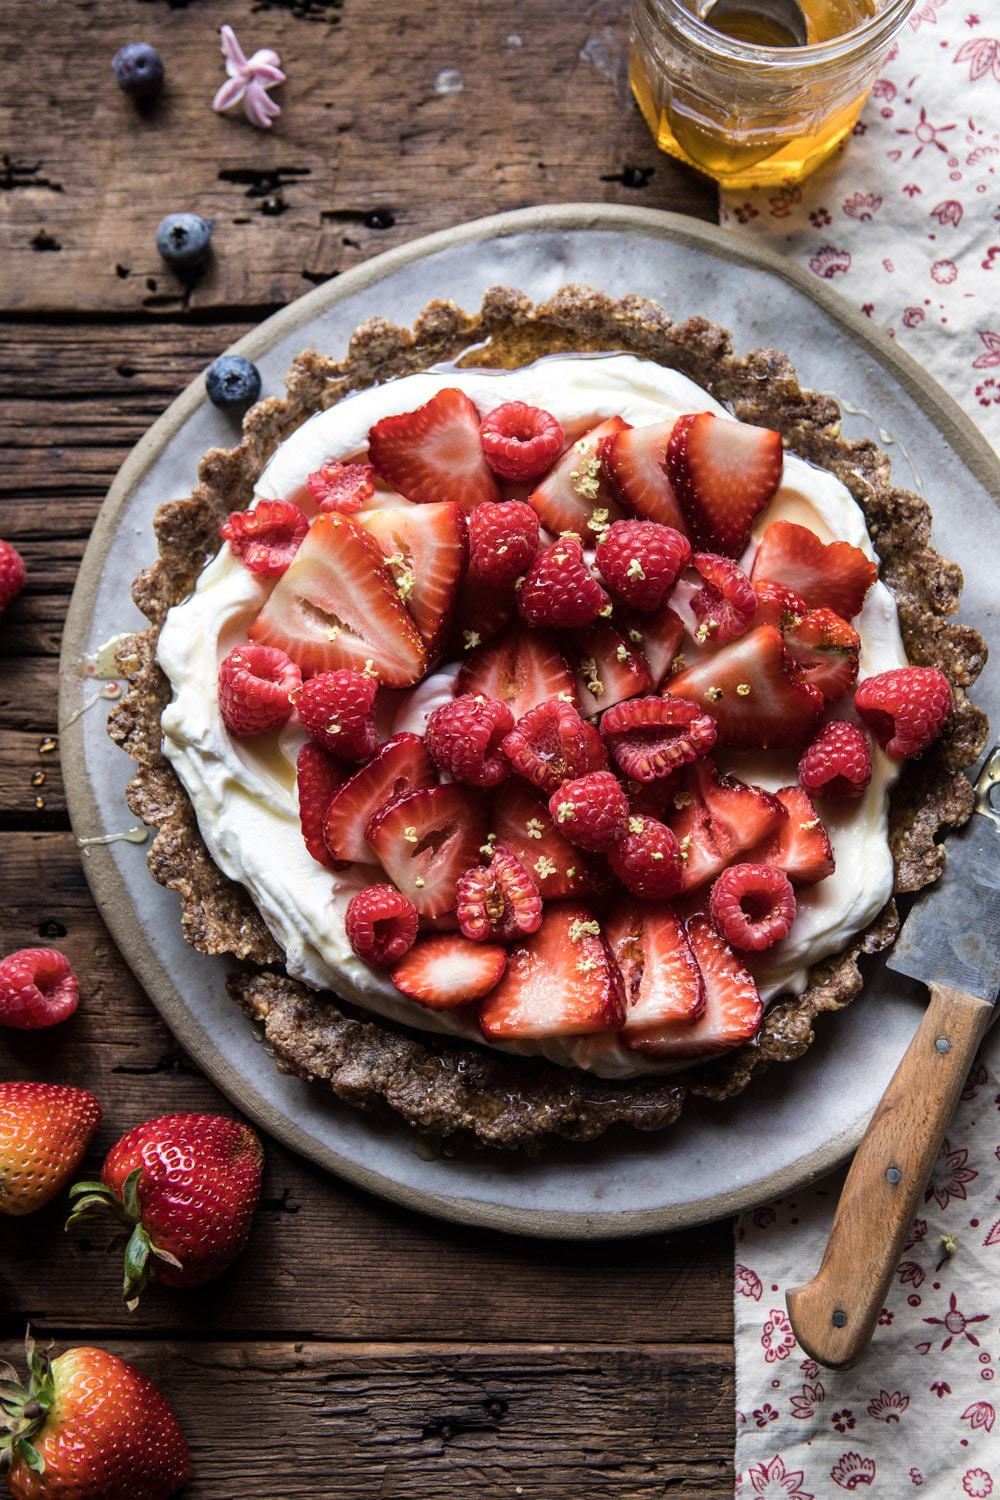
\includegraphics[width=1\textwidth,height=\textheight]{images/no-bake-greek-yogurt-fruit-tart.jpg}

\textbf{Prep Time:} 15 min \textbar{} \textbf{Cook Time:} 10 min
\textbar{} \textbf{Total Time:} 25 min

\section{Ingredients}\label{ingredients-10}

\begin{itemize}
\tightlist
\item
  2 cups raw pecans
\item
  10 Medjool dates, pitted
\item
  1 pinch flaky salt
\item
  1 ½ cups plain Greek yogurt
\item
  1 cup fresh raspberries, blueberries, or blackberries
\item
  6 strawberries, sliced
\item
  2 tablespoons honey
\end{itemize}

\section{Instructions}\label{instructions-10}

\begin{enumerate}
\def\labelenumi{\arabic{enumi}.}
\tightlist
\item
  To make the crust. In a food processor, pulse the pecans until ground
  into a semi-fine meal. Add the dates and salt and pulse until the
  mixture holds together when pinched and starts to look like dough.
\item
  Press the dough into an 8 or 9 inch tart pan with a removable bottom
  to form a flat, even crust. Chill in the freezer for 10 minutes or up
  to 1 week.
\item
  To make the filling. Remove the crust from the freezer and carefully
  slide it onto a serving plate. Spread the yogurt over the crust. Top
  the yogurt with the berries, then drizzle with honey. Slice and serve.
\end{enumerate}

\bookmarksetup{startatroot}

\chapter{Easiest Pistachio Chocolate
Baklava}\label{easiest-pistachio-chocolate-baklava}

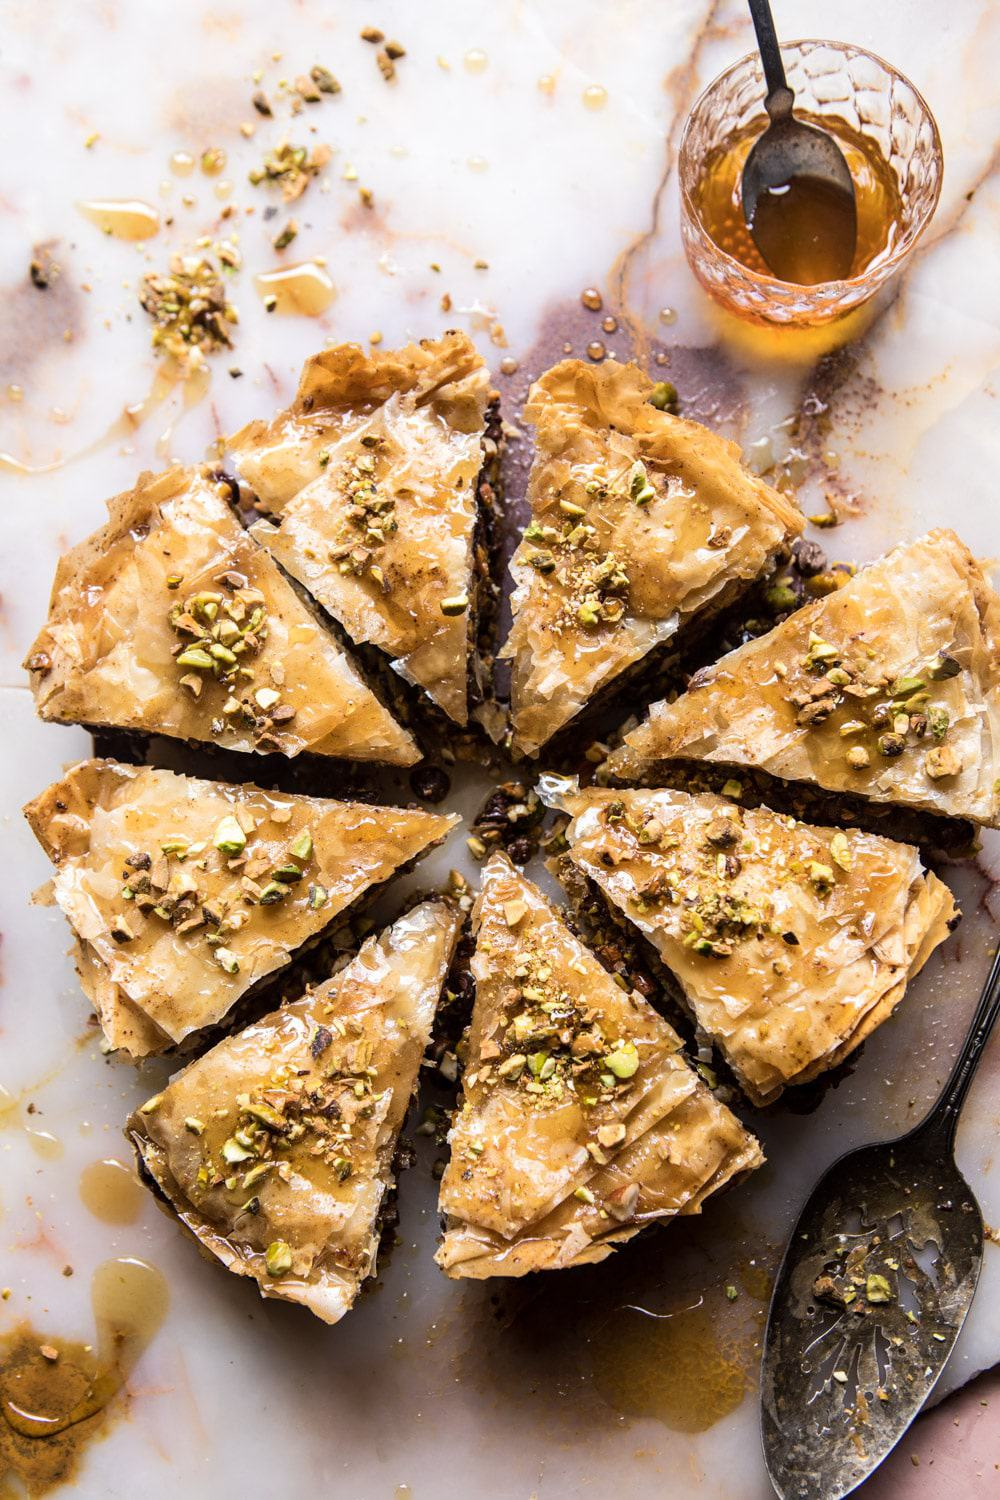
\includegraphics[width=1\textwidth,height=\textheight]{images/easiest-pistachio-chocolate-baklava.jpg}

\textbf{Prep Time:} 20 min \textbar{} \textbf{Cook Time:} 45 min
\textbar{} \textbf{Total Time:} 1 hr 5 min

\section{Ingredients}\label{ingredients-11}

\begin{itemize}
\tightlist
\item
  2 cups pistachios, roasted, salted, and roughly chopped
\item
  1 cup almonds, roasted or raw, and roughly chopped
\item
  1 1/2 cups semi-sweet chocolate chips
\item
  1/2 teaspoon cinnamon
\item
  24 sheets frozen phyllo dough, thawed (about 1/2 a pound)
\item
  1 stick salted butter, melted
\item
  1 cup honey
\item
  2 teaspoons vanilla extract
\end{itemize}

\section{Instructions}\label{instructions-11}

\begin{enumerate}
\def\labelenumi{\arabic{enumi}.}
\tightlist
\item
  Preheat the oven to 350 degrees F. Line a 9 inch spring form pan with
  parchment paper.
\item
  In a medium bowl, combine the pistachios, almonds, chocolate chips,
  and cinnamon.
\item
  Fold 1 sheet of phyllo dough in half and then place in the prepared
  pan. Brush the phyllo dough with melted butter. Repeat, layering 8
  more times, placing the sheets of dough over top of each other. Spoon
  half of the nut/chocolate mix over the dough. Now add another 8 sheets
  of phyllo, brushing each with butter. Spoon over the remaining
  filling. Add another 8 sheet of phyllo, agin brushing each with
  butter.
\item
  Cut the baklava into 8 triangles. Place the pan on a baking sheet and
  transfer to the oven and bake for 45-50 minutes, until phyllo is
  golden brown.
\item
  Meanwhile, combine 1/2 cup water and the honey in a medium saucepan
  and bring to a boil. Reduce the heat and simmer 5 minutes until
  thickened slightly. Remove from the heat and stir in the vanilla. Pour
  the syrup over the warm baklava and let soak for 2 hour or overnight.
  Enjoy!
\end{enumerate}

\bookmarksetup{startatroot}

\chapter{Sun-Dried Tomato, White Bean, and Goat Cheese
Pasta}\label{sun-dried-tomato-white-bean-and-goat-cheese-pasta}

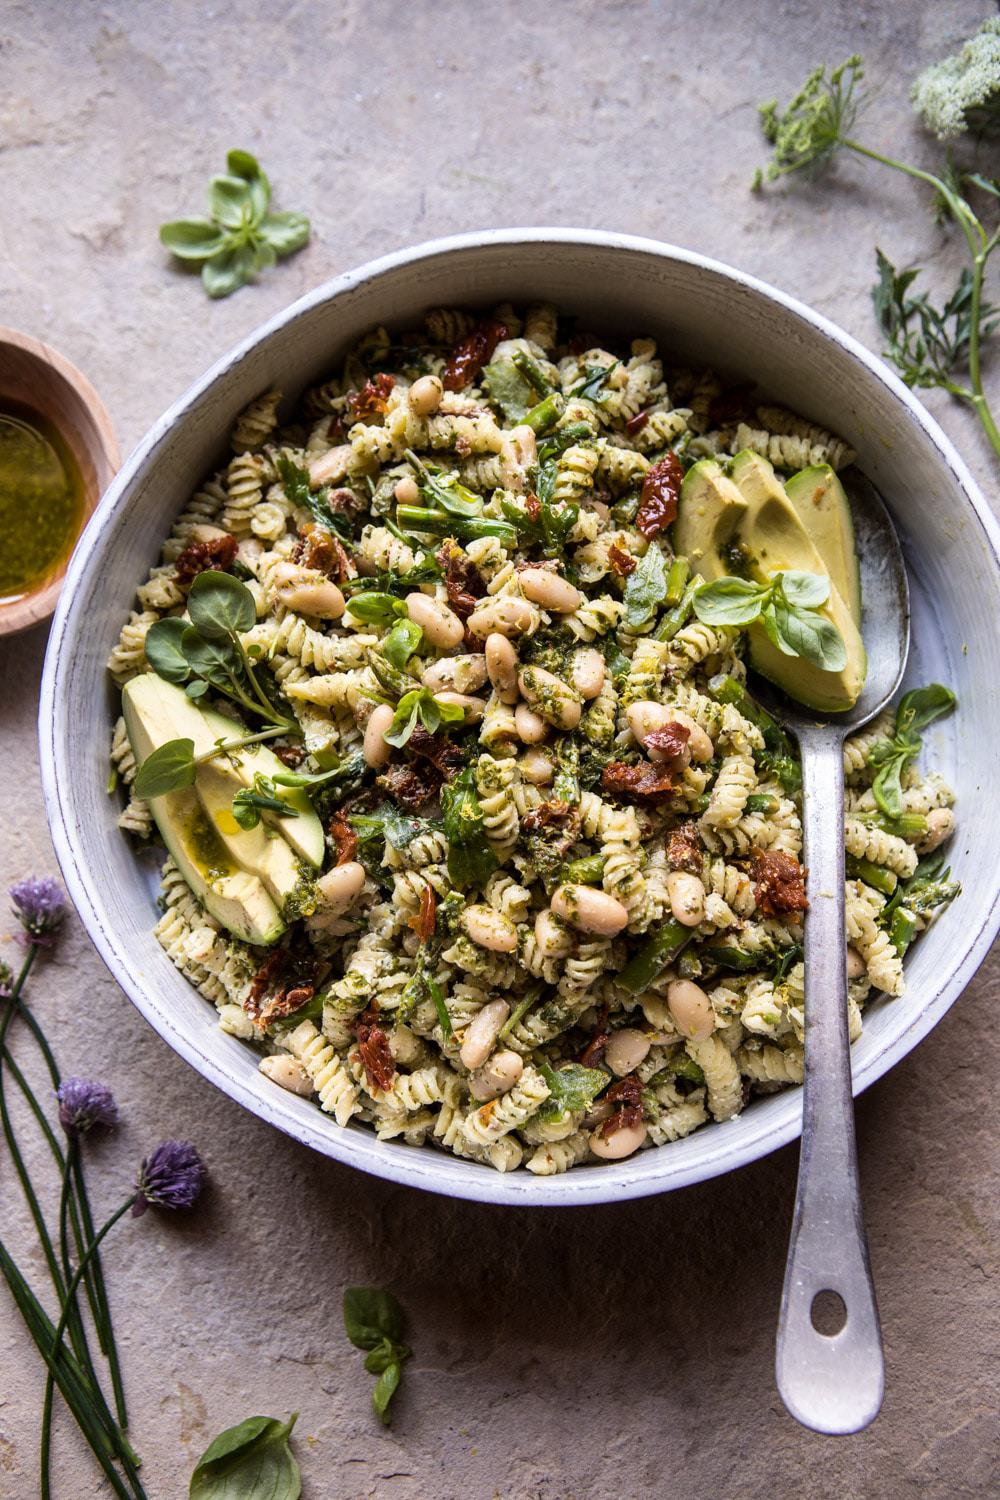
\includegraphics[width=1\textwidth,height=\textheight]{images/sun-dried-tomato-white-bean-and-goat-cheese-pasta.jpg}

\textbf{Prep Time:} 15 min \textbar{} \textbf{Cook Time:} 10 min
\textbar{} \textbf{Total Time:} 25 min

\section{Ingredients}\label{ingredients-12}

\begin{itemize}
\tightlist
\item
  1/2 cup extra virgin olive oil
\item
  1 cup fresh basil
\item
  2 fresh chives
\item
  2 sprigs fresh dill
\item
  2 tablespoons lemon juice
\item
  1 tablespoon red wine vinegar
\item
  1 clove garlic, smashed
\item
  1/2 teaspoon crushed red pepper flakes, or more to taste
\item
  kosher salt
\item
  1 pound short cut pasta
\item
  1 bunch asparagus, cut into 1 inch pieces
\item
  4-6 ounces soft goat cheese, crumbled
\item
  1 jar (8 ounces) oil packed sun-dried tomatoes chopped
\item
  1 can (14 ounces) white beans, drained
\item
  1 avocado, sliced
\end{itemize}

\section{Instructions}\label{instructions-12}

\begin{enumerate}
\def\labelenumi{\arabic{enumi}.}
\tightlist
\item
  To make the vinaigrette. In a blender, combine the olive oil, basil,
  chives, dill, lemon juice, vinegar, garlic, 1 teaspoon of the salt,
  and a pinch red pepper flakes until smooth. Taste and adjust salt as
  needed.
\item
  Bring a large pot of salted water to a boil. Boil the pasta to al
  dente, according to package directions. During the last 2-3 minutes of
  cooking, add the asparagus to the water. Drain and add to a serving
  bowl.
\item
  Toss the hot pasta and asparagus with the goat cheese and a couple
  large spoonfuls of the basil vinaigrette, toss well until the goat
  cheese coats the pasta completely. Add the sun-dried tomatoes and
  white beans, tossing to combine. Top the pasta with avocado. Serve the
  remaining vinaigrette on the side.
\end{enumerate}

\bookmarksetup{startatroot}

\chapter{Parchment Baked Lemon Salmon and Potatoes with Dill
Yogurt}\label{parchment-baked-lemon-salmon-and-potatoes-with-dill-yogurt}

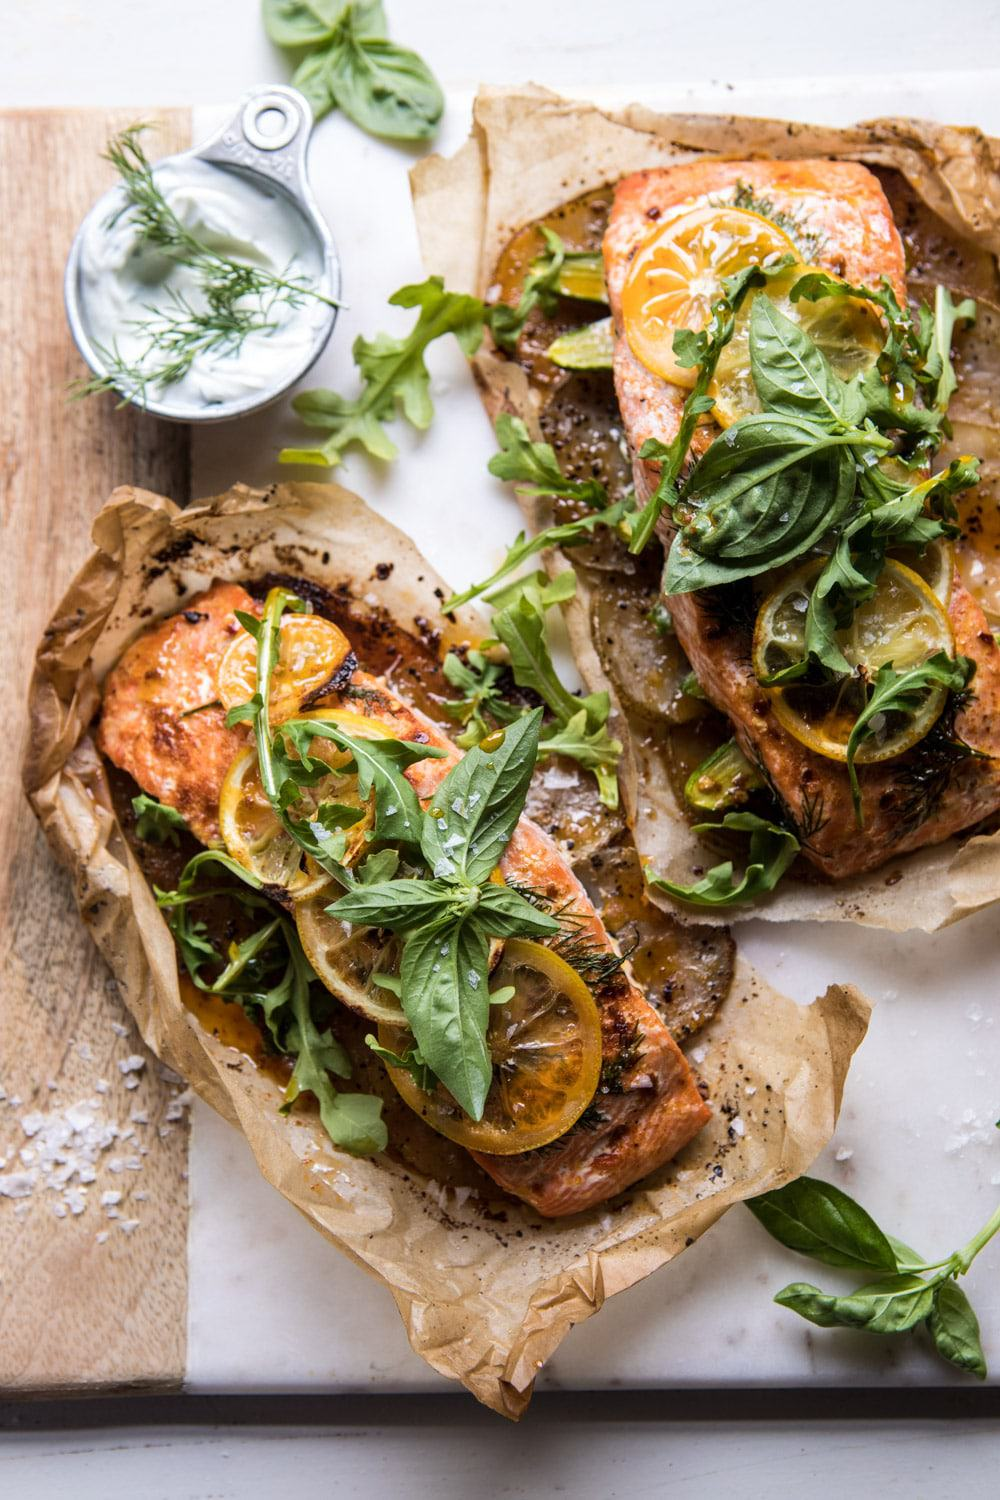
\includegraphics[width=1\textwidth,height=\textheight]{images/parchment-baked-lemon-salmon-and-potatoes-with-dill-yogurt.jpg}

\textbf{Prep Time:} 10 min \textbar{} \textbf{Cook Time:} 20 min
\textbar{} \textbf{Total Time:} 30 min

\section{Ingredients}\label{ingredients-13}

\begin{itemize}
\tightlist
\item
  1/4 cup extra virgin olive oil
\item
  2 cloves garlic, minced or grated
\item
  2 lemons
\item
  1 tablespoon chopped fresh dill
\item
  2 teaspoons smoked paprika
\item
  2 small potatoes, very thinly sliced using a mandolin
\item
  4 6-8 ounce salmon fillets, skinned
\item
  kosher salt and pepper
\item
  fresh arugula and basil, for serving
\item
  1 cup plain greek yogurt
\item
  1 tablespoon chopped fresh dill
\item
  juice of 1 lemon
\item
  1 pinch crushed red pepper flakes
\end{itemize}

\section{Instructions}\label{instructions-13}

\begin{enumerate}
\def\labelenumi{\arabic{enumi}.}
\tightlist
\item
  Preheat the oven to 400 degrees F. Fold 4 large pieces of parchment
  paper (about 15x16 inches) in half. Open, and lay on half flat.
\item
  In a small bowl, stir together the olive oil, garlic, juice of 1
  lemon, dill, smoked paprika and a pinch of salt and pepper.
\item
  Working on one side of the creased parchment, layer the potatoes, and
  season with salt and pepper. Place the salmon over the potatoes and
  drizzle with the olive oil sauce, and top with 2 lemons slices. Repeat
  with the remaining ingredients to make 4 packets.
\item
  To close, fold the parchment over salmon, pinching to seal the open
  sides and create a half-moon-shaped packet. Place on a rimmed baking
  sheet. Transfer to the oven and bake until the potatoes are tender,
  about 18-20 minutes.
\item
  Meanwhile, in a medium bowl, stir together the yogurt, lemon juice,
  dill, and a pinch of crushed red pepper.
\item
  Serve the salmon topped with dill yogurt, arugula, and basil. Enjoy!
\end{enumerate}

\bookmarksetup{startatroot}

\chapter{Spring Chicken Parmesan with Tuscan Kale
Pesto}\label{spring-chicken-parmesan-with-tuscan-kale-pesto}

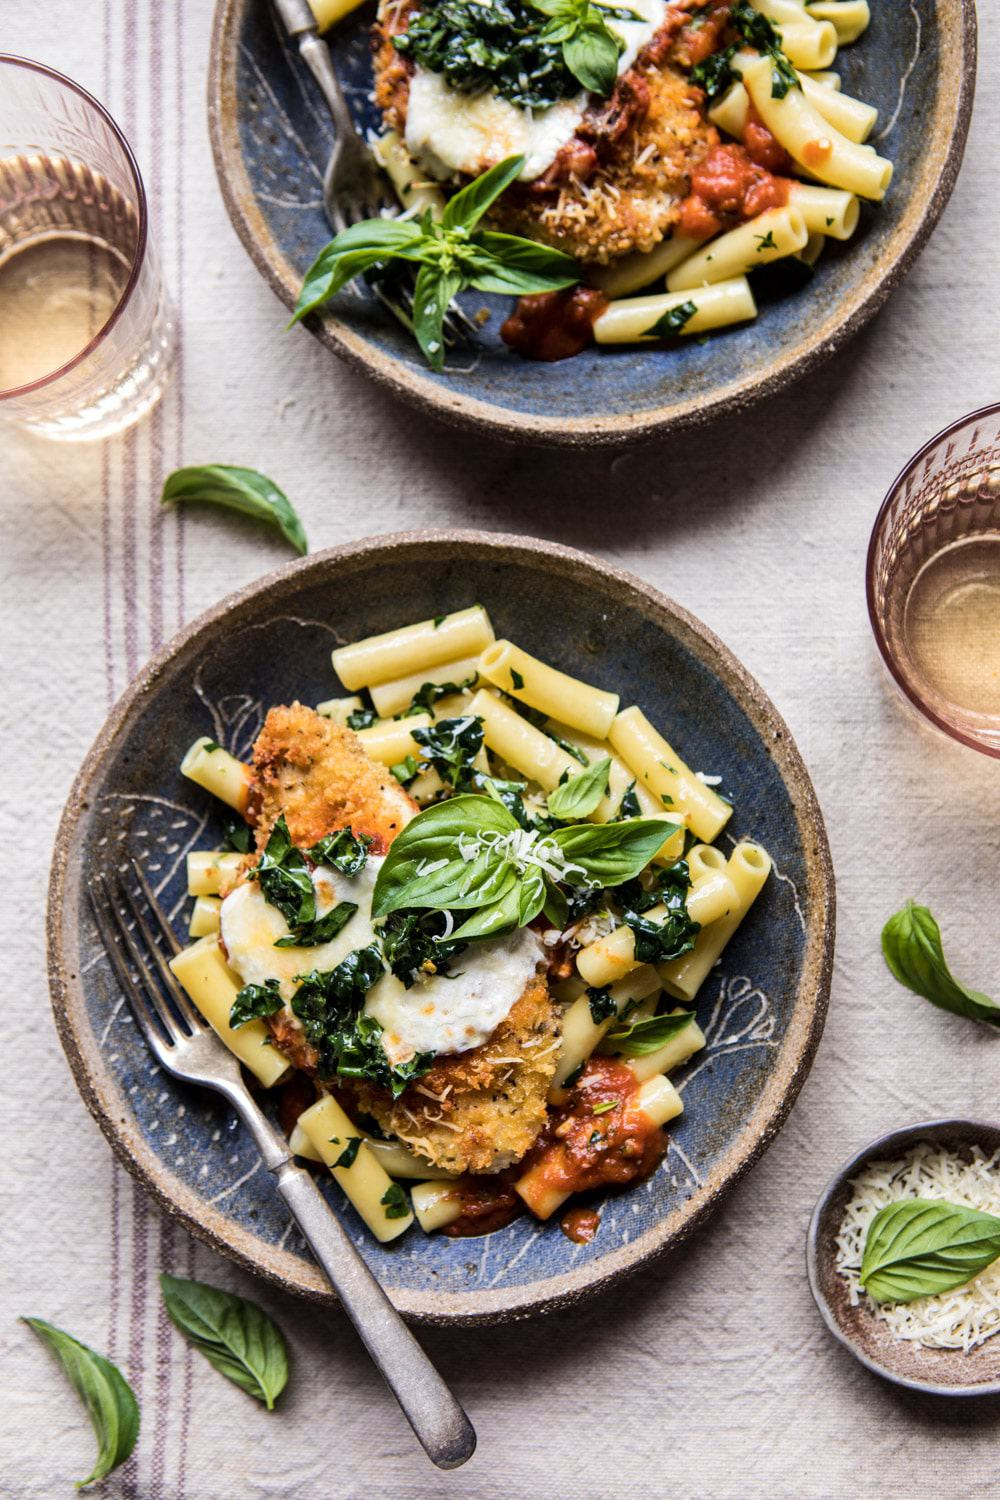
\includegraphics[width=1\textwidth,height=\textheight]{images/spring-chicken-parmesan-with-tuscan-kale-pesto.jpg}

\textbf{Prep Time:} 20 min \textbar{} \textbf{Cook Time:} 20 min
\textbar{} \textbf{Total Time:} 40 min

\section{Ingredients}\label{ingredients-14}

\begin{itemize}
\tightlist
\item
  3 boneless, skinless chicken breasts, sliced in half horizontally
\item
  3 tablespoons extra virgin olive oil, plus more for the pan
\item
  kosher salt and pepper
\item
  1 cup panko bread crumbs
\item
  1 cup grated parmesan cheese, plus more for serving
\item
  1 teaspoon dried oregano
\item
  1 jar (23 ounces) Bertolli® Rustic Cut Pasta Sauce
\item
  1 cup shredded mozzarella cheese
\item
  fresh basil and arugula, for serving
\item
  pasta, for serving
\item
  1 cup roughly chopped kale
\item
  1 cup fresh basil
\item
  2 tablespoons toasted pine nuts
\item
  1/3 cup grated parmesan cheese
\item
  1/4 cup olive oil
\item
  2 tablespoons lemon juice
\item
  kosher salt
\end{itemize}

\section{Instructions}\label{instructions-14}

\begin{enumerate}
\def\labelenumi{\arabic{enumi}.}
\tightlist
\item
  Preheat the oven to 400 degrees F.
\item
  Toss the chicken with olive oil and season with salt and pepper.
\item
  Add the bread crumbs, 1/2 cup parmesan cheese, and oregano to a
  shallow bowl. Working with 1 piece of chicken at a time, dredge
  through the bread crumbs. Repeat with the remaining chicken.
\item
  Heat a drizzle of olive oil in a large oven safe skillet over medium
  heat. When the oil simmers, add the chicken and cook for 1-2 minutes
  per side or until golden. Remove from the heat. Spoon a couple
  spoonfuls of pasta sauce over each piece of chicken and then top
  evenly with mozzarella and the remaining 1/2 cup parmesan.
\item
  Transfer the skillet to the oven and bake for 10 minutes or until the
  cheese is melted and the chicken is cooked through.
\item
  Serve the chicken over a bed of pasta with additional pasta sauce. Top
  each piece of chicken with kale pesto and fresh greens. Enjoy!
\end{enumerate}

\bookmarksetup{startatroot}

\chapter{Whole Wheat Chocolate Chip Skillet
Cookie}\label{whole-wheat-chocolate-chip-skillet-cookie}

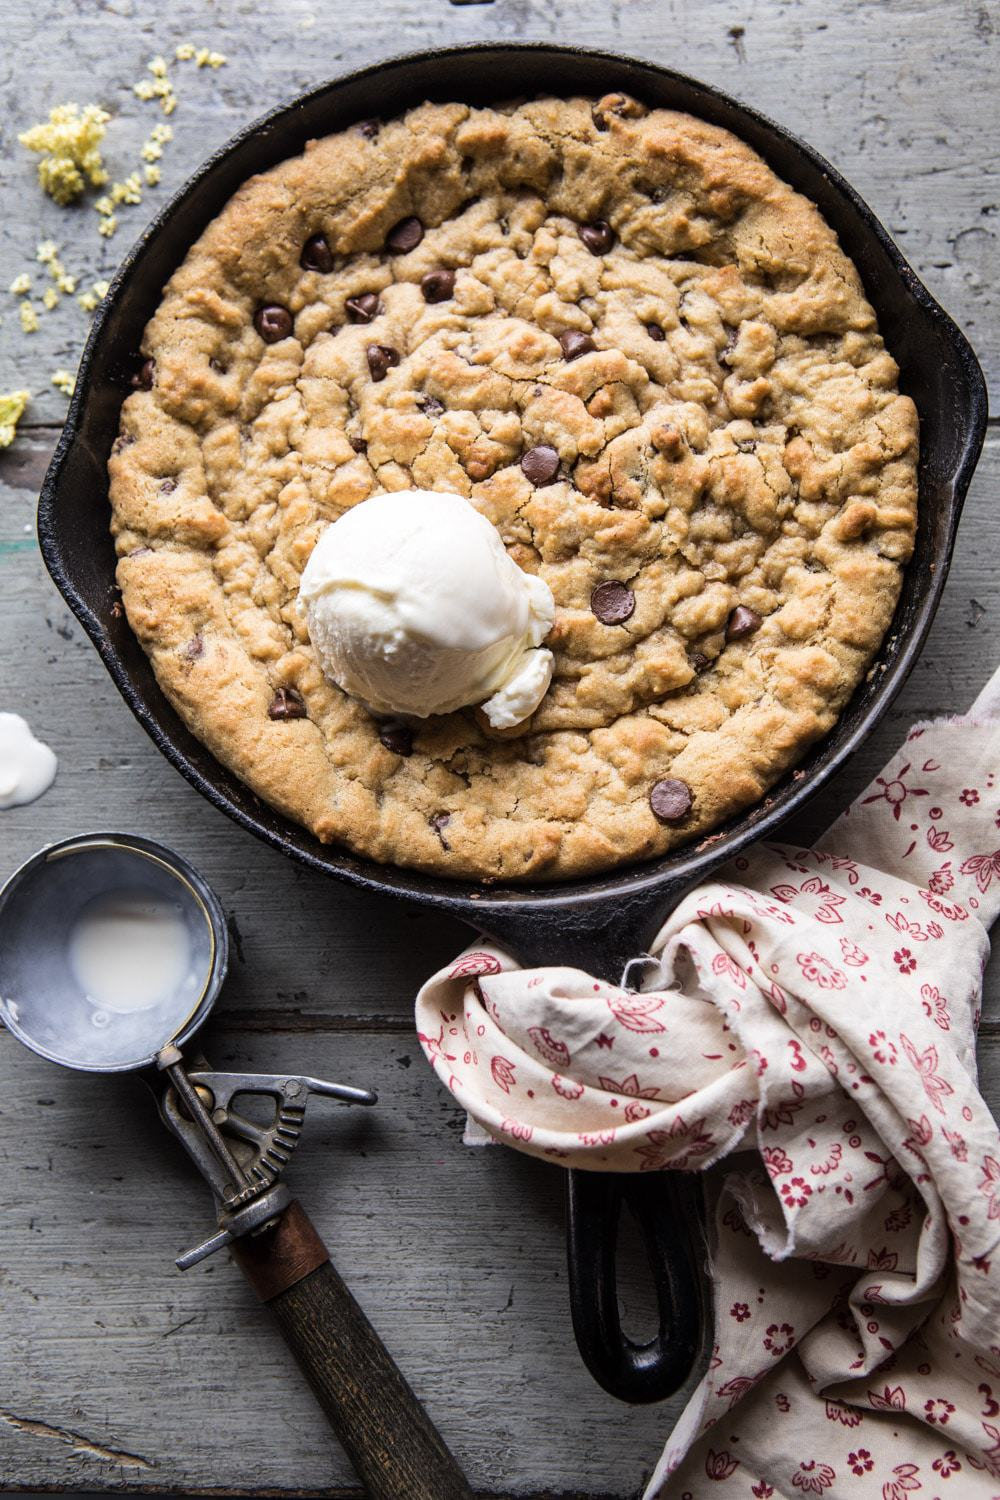
\includegraphics[width=1\textwidth,height=\textheight]{images/whole-wheat-chocolate-chip-skillet-cookie.jpg}

\textbf{Prep Time:} 10 min \textbar{} \textbf{Cook Time:} 20 min
\textbar{} \textbf{Total Time:} 30 min

\section{Ingredients}\label{ingredients-15}

\begin{itemize}
\tightlist
\item
  1 1/2 sticks (3/4 cup) salted grass-fed butter, softened
\item
  2 eggs
\item
  3/4 cup real maple syrup
\item
  2 teaspoons vanilla extract
\item
  2 cups white whole wheat flour or whole wheat pastry flour
\item
  1 teaspoon baking soda
\item
  1 1/2 cups dark or semi-sweet chocolate chips
\end{itemize}

\section{Instructions}\label{instructions-15}

\begin{enumerate}
\def\labelenumi{\arabic{enumi}.}
\tightlist
\item
  Preheat the oven to 350 degrees F. Grease a 10-12 inch oven safe
  skillet with butter.
\item
  In a large mixing bowl, beat the butter until light, and fluffy. Add
  the eggs, one at a time, until combined. Slowly add in the maple and
  vanilla, beating until combined. Add the flour and baking soda and
  beat until fully incorporated. Stir in the chocolate chips.
\item
  Spread the dough out in the prepared skillet. Transfer to the oven and
  bake for 18-20 minutes, it's OK if the center is a little gooey.
  Remove from the oven, let cool 3-5 minutes. DIG in, preferably with a
  scoop of ice cream.
\end{enumerate}

\bookmarksetup{startatroot}

\chapter{Thai Basil Steak Salad
Sandwich.}\label{thai-basil-steak-salad-sandwich.}

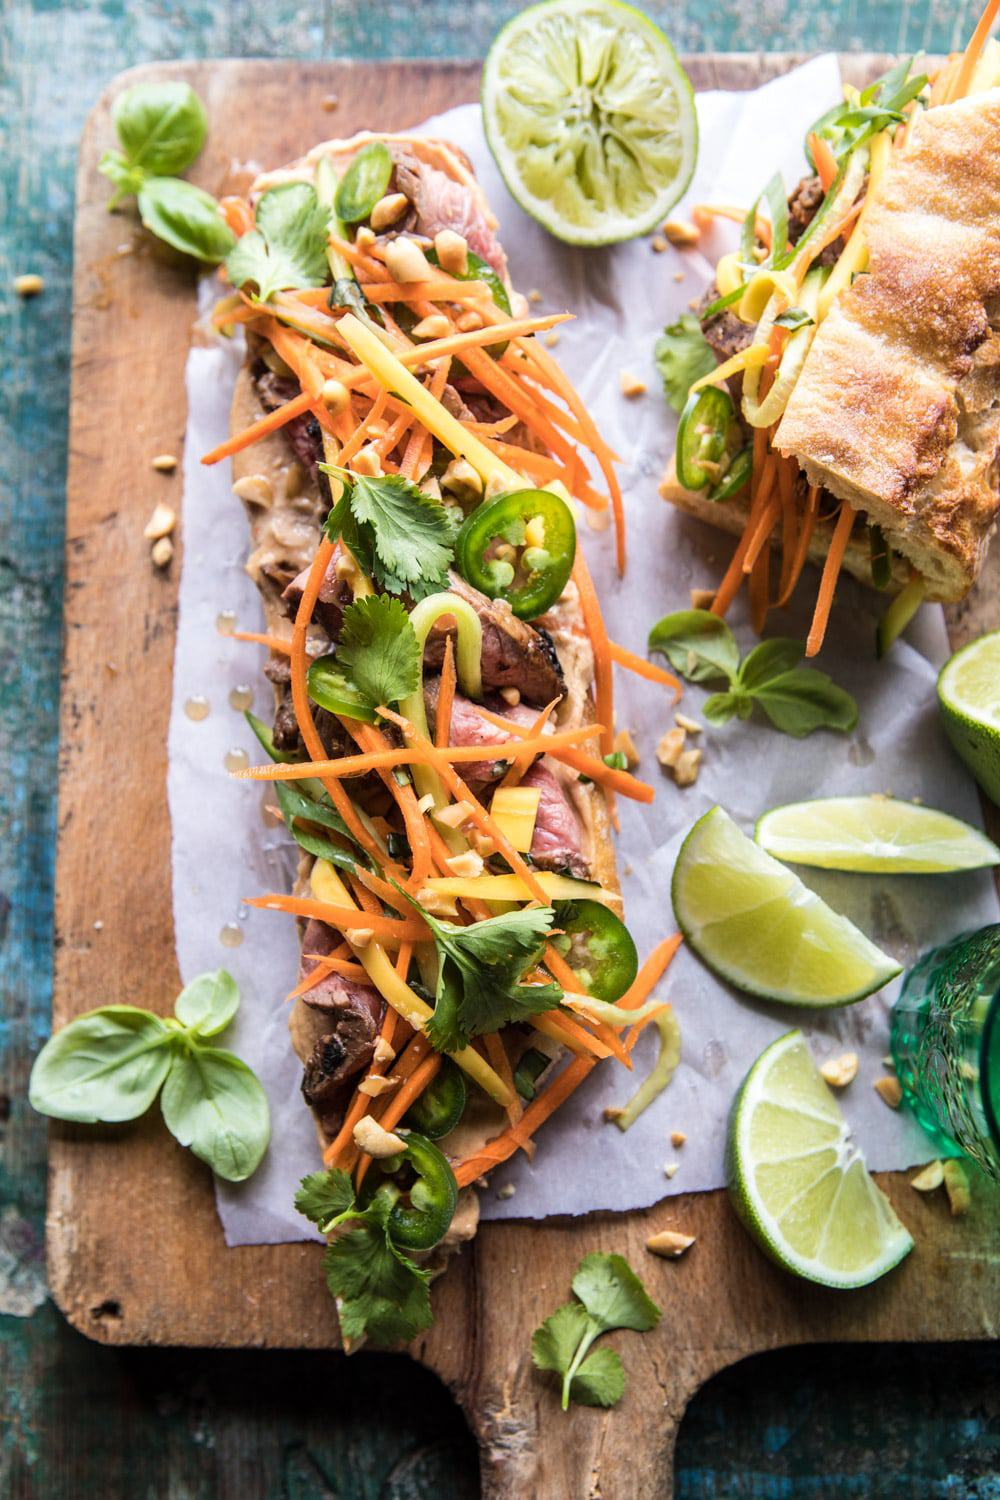
\includegraphics[width=1\textwidth,height=\textheight]{images/thai-basil-steak-salad-sandwich-.jpg}

\textbf{Prep Time:} 20 min \textbar{} \textbf{Cook Time:} 10 min
\textbar{} \textbf{Total Time:} 30 min

\section{Ingredients}\label{ingredients-16}

\begin{itemize}
\tightlist
\item
  2 pounds skirt steak
\item
  1/4 cup extra virgin olive oil
\item
  1/3 cup honey
\item
  1/3 cup low sodium soy sauce or tamari
\item
  4 cloves garlic, minced or grated
\item
  1 inch fresh ginger, grated
\item
  1 tablespoon chili paste
\item
  1 toasted baguette, halved and cut into 4-6 pieces
\item
  gingered tahini or mayo, for spreading ((optional))
\item
  1/3 cup sesame oil
\item
  juice from 2 limes
\item
  1 tablespoon fish sauce
\item
  2 green onions, chopped
\item
  1/3 cup fresh basil, chopped
\item
  1/4 cup fresh cilantro, chopped
\item
  1 mango, sliced or chopped
\item
  2 carrots, shredded
\item
  2 persian cucumbers, sliced
\item
  2 jalapeños, sliced
\item
  1/4 cup roasted peanuts, chopped
\end{itemize}

\section{Instructions}\label{instructions-16}

\begin{enumerate}
\def\labelenumi{\arabic{enumi}.}
\tightlist
\item
  Add the steak to a ziplock bag, then add the olive oil, honey, soy
  sauce, garlic, ginger, and chili paste. Seal the bag and marinate 30
  minutes or in the fridge as long as overnight.
\item
  Meanwhile, in a medium to large bowl, combine the sesame oil, lime
  juice, fish sauce, green onions, basil, cilantro, mangos, carrots,
  cucumbers, and jalapeños. Toss to combine.
\item
  Preheat your grill or grill pan to high.
\item
  Remove the steak from its marinade and sear the steak for 5-8 minutes,
  flip and sear another 5 minutes or until your desired doneness is
  reached. Remove the steak from the grill and allow to rest 10 minutes.
  Slice steak thinly against the grain.
\item
  Spread the toasted baguette with tahini. Top with sliced steak and
  salad. Sprinkle with peanuts. Enjoy!
\end{enumerate}

\bookmarksetup{startatroot}

\chapter{Chipotle Lime Chicken and Sweet Potato Salad with Jalapeño
Vinaigrette}\label{chipotle-lime-chicken-and-sweet-potato-salad-with-jalapeuxf1o-vinaigrette}

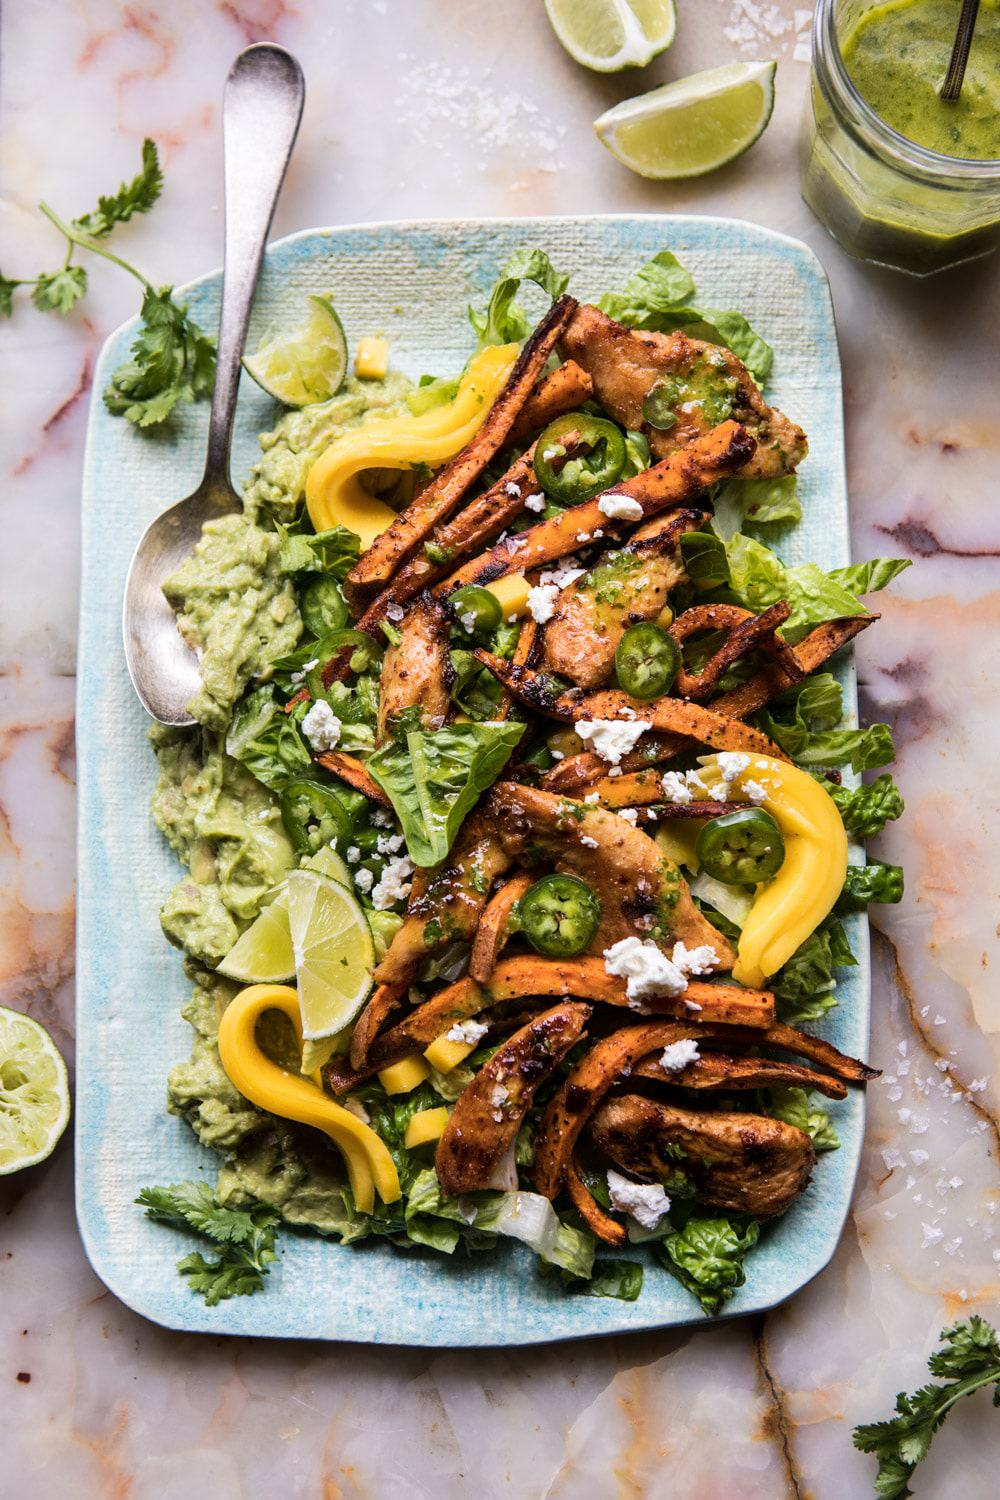
\includegraphics[width=1\textwidth,height=\textheight]{images/chipotle-lime-chicken-and-sweet-potato-salad-with-jalape-o-vinaigrette.jpg}

\textbf{Prep Time:} 15 min \textbar{} \textbf{Cook Time:} 30 min
\textbar{} \textbf{Total Time:} 45 min

\section{Ingredients}\label{ingredients-17}

\begin{itemize}
\tightlist
\item
  1 pound boneless chicken breasts, cut into strips
\item
  4 tablespoons extra virgin olive oil
\item
  2 chipotle peppers in adobo, chopped
\item
  1 tablespoon honey
\item
  1 teaspoon cumin
\item
  2 limes
\item
  2 cloves garlic, minced or grated
\item
  kosher salt and pepper
\item
  2 sweet potatoes, cut into matchsticks
\item
  2 avocados, lightly mashed
\item
  3 heads romaine lettuce chopped
\item
  1 mango, diced
\item
  8 ounces feta, crumbled
\item
  1/3 cup extra virgin olive oil
\item
  1/3 cup fresh orange juice
\item
  2 tablespoons lime juice
\item
  1/2 cup fresh cilantro
\item
  1 jalapeño, halved and seeded if desired
\item
  kosher salt and pepper
\end{itemize}

\section{Instructions}\label{instructions-17}

\begin{enumerate}
\def\labelenumi{\arabic{enumi}.}
\tightlist
\item
  Preheat the oven to 425 degrees F.
\item
  On a rimmed baking sheet, combine the chicken, 2 tablespoons olive
  oil, chipotle, honey, cumin, juice and zest of 1 lime, garlic and a
  large pinch of both salt and pepper. Toss well to evenly coat the
  chicken.
\item
  On a separate baking sheet, toss together the sweet potatoes and
  remaining 2 tablespoons olive oil, plus a pinch of both salt and
  pepper. Roast both the chicken and potatoes for 25-30 minutes, tossing
  halfway through cooking until the chicken is cooked throughout and the
  potatoes tender.
\item
  In a medium bowl, stir together the avocados, remaining lime juice and
  a pinch of salt.
\item
  In a large salad bowl, toss together the lettuce, mango, feta, fries,
  and chicken. Dollop the avocado over the salad. Drizzle with
  vinaigrette (recipe follows).
\item
  Add all ingredients to a blender and blend until combined. Taste and
  adjust seasonings as needed. The vinaigrette can be made a few days in
  advance and kept in the fridge.
\end{enumerate}

\bookmarksetup{startatroot}

\chapter{Zucchini, Bacon, and Pecorino
Tart}\label{zucchini-bacon-and-pecorino-tart}

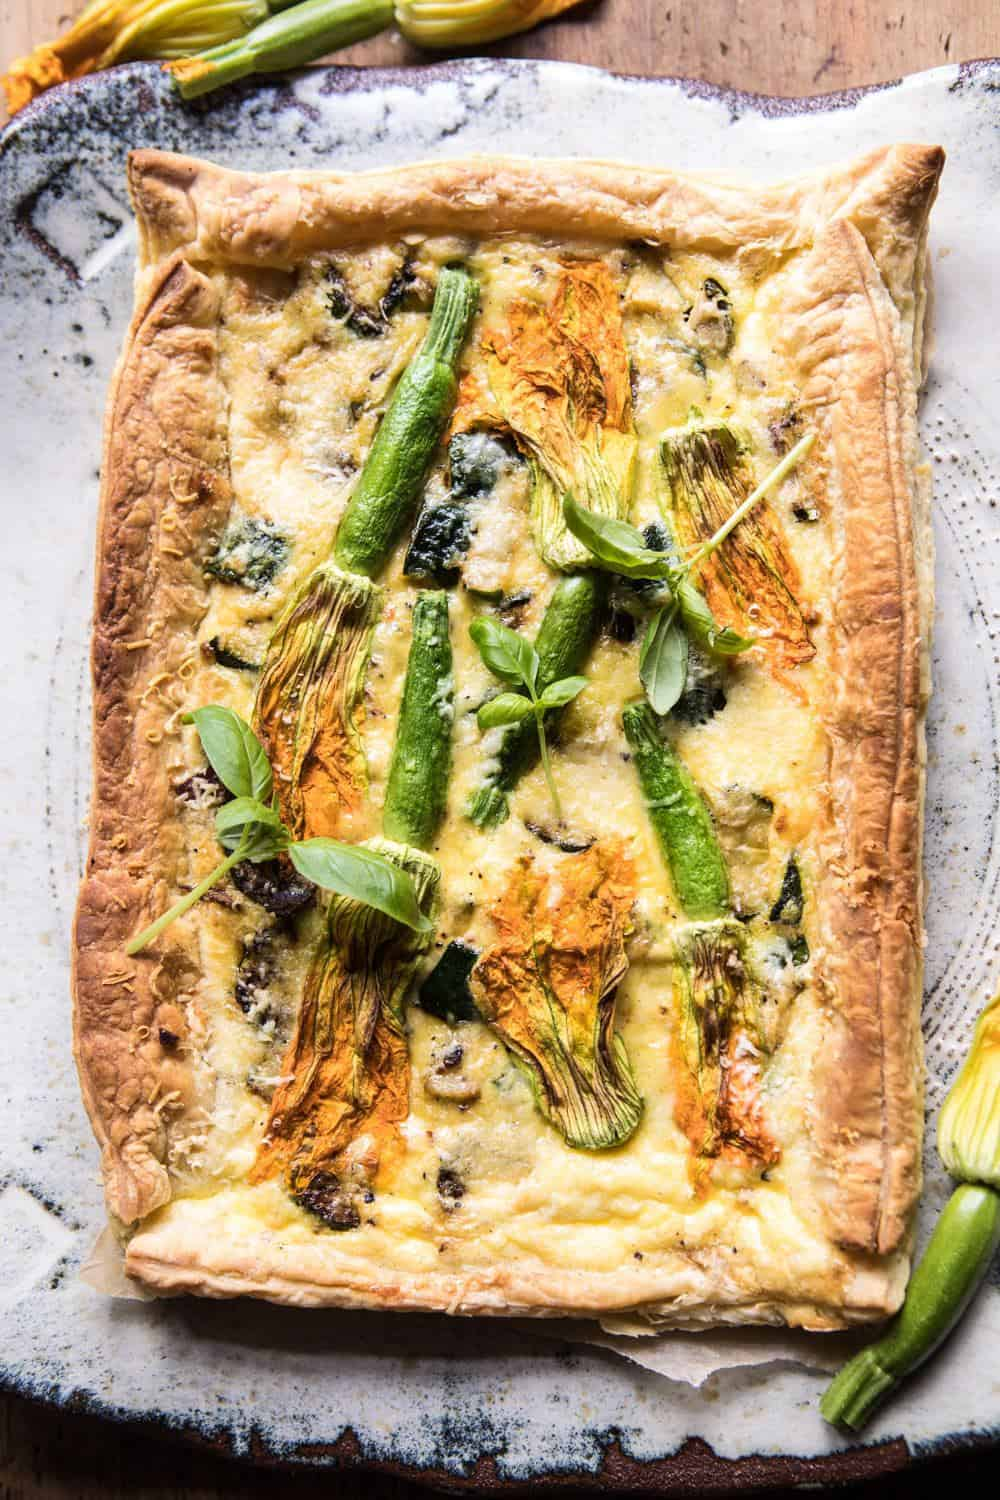
\includegraphics[width=1\textwidth,height=\textheight]{images/zucchini-bacon-and-pecorino-tart.jpg}

\textbf{Prep Time:} 20 min \textbar{} \textbf{Cook Time:} 1 hr
\textbar{} \textbf{Total Time:} 1 hr 20 min

\section{Ingredients}\label{ingredients-18}

\begin{itemize}
\tightlist
\item
  1 sheet frozen puff pastry, thawed
\item
  3-4 medium zucchini, chopped
\item
  1 tablespoon extra virgin olive oil
\item
  kosher salt
\item
  1/2 cup cubed bacon or pancetta
\item
  3 large eggs
\item
  1/2 cup heavy cream
\item
  1/2 cup grated pecorino cheese
\item
  zucchini blossoms, for topping ((optional))
\end{itemize}

\section{Instructions}\label{instructions-18}

\begin{enumerate}
\def\labelenumi{\arabic{enumi}.}
\tightlist
\item
  Preheat the oven to 400 degrees. Grease a 9-inch tart pan with a
  little butter or oil, then dust it with flour until well coated.
\item
  Roll out the puff pastry into a large circle and drape it over the
  tart pan. Press the pastry into the nooks and crannies, then roll a
  rolling-pin over the top to cut away the excess pastry. Cover the
  pastry with a sheet of parchment paper and fill it with baking beans
  or weights. Set the pan in the oven and bake for 15 minutes, until dry
  to the touch. Remove from the oven, discard the parchment paper and
  baking beans, and bake for 3 to 5 minutes more to crisp up the base.
\item
  Meanwhile, roughly slice the zucchini into 1 inch thick rounds.
  Drizzle the olive oil into a large saucepan, set on medium heat, and
  add the zucchini and salt. Cook, stirring until the zucchini begin to
  color very lightly, 3 to 5 minutes. Toss in the pancetta and cook,
  stirring until the pancetta is crisp, 3 to 5 minutes more.
\item
  In a large bowl, whisk the eggs and cream with a fork, then whisk in
  the cheese. Season with a little salt. Allow the pancetta and zucchini
  mixture to cool a little (so that it doesn’t cook the eggs), then add
  it to the eggs and cheese, and toss well.
\item
  Pour the filling into the prepared pastry shell. If using, open the
  zucchini blossoms very gently and pull out and discard the stamens.
  Then arrange the flowers on the top of the pie, gently pressing them
  into the filling. Bake the pie for 20 to 25 minutes, until golden on
  top. It’s delicious eaten warm from the oven, or at room temperature.
\end{enumerate}

\bookmarksetup{startatroot}

\chapter{Spring Skillet Roasted Lemon Chicken and
Veggies}\label{spring-skillet-roasted-lemon-chicken-and-veggies}

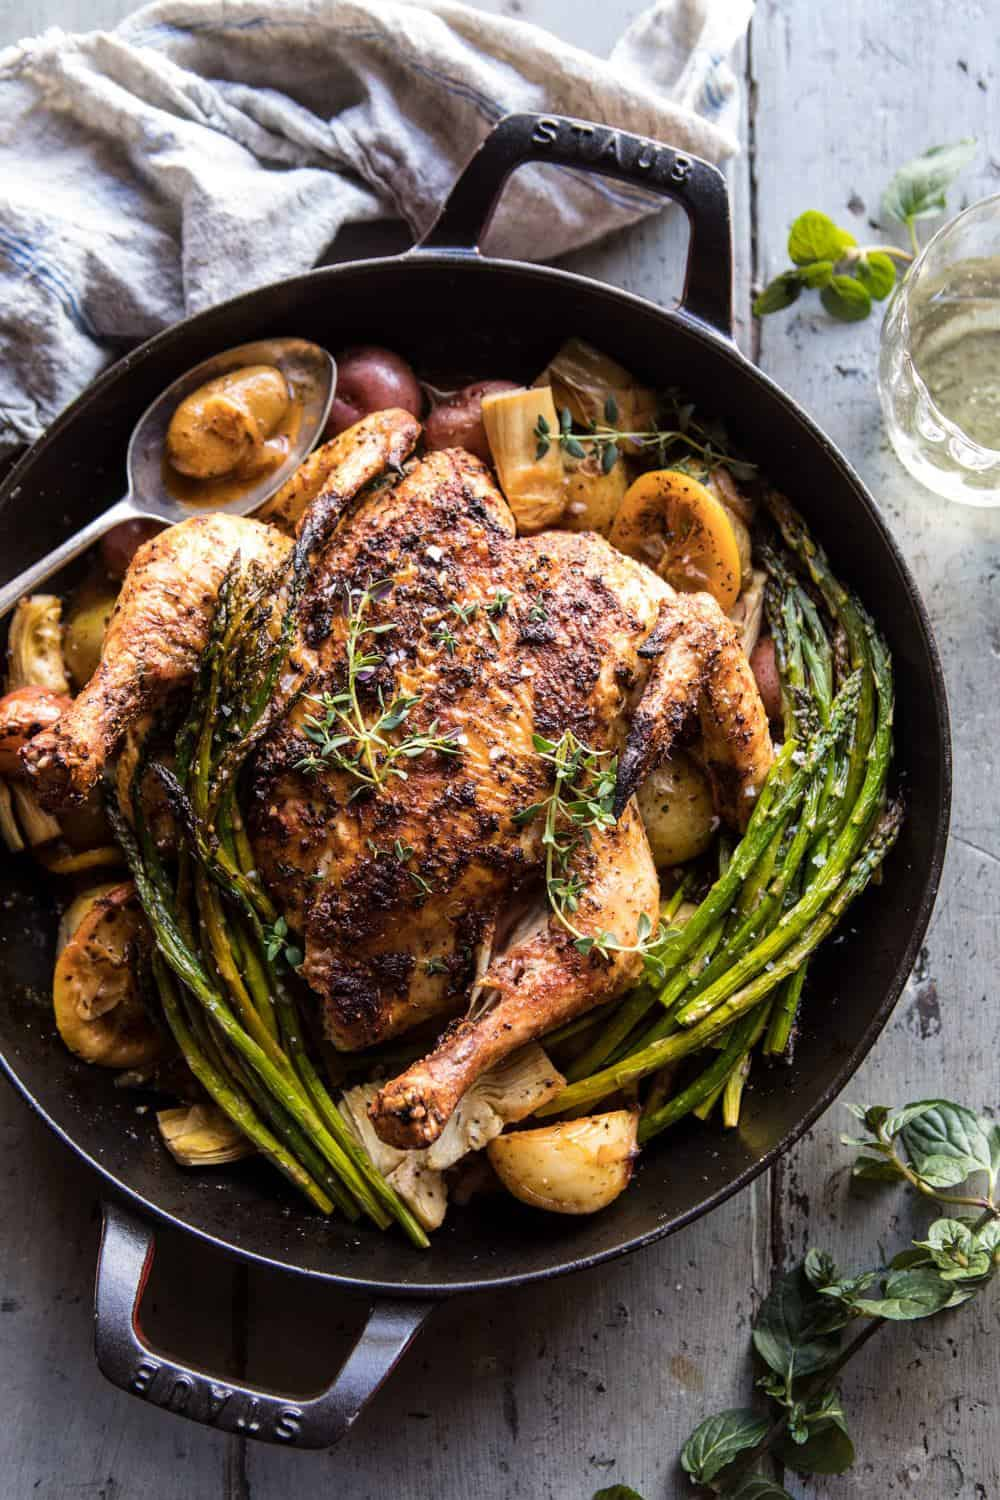
\includegraphics[width=1\textwidth,height=\textheight]{images/spring-skillet-roasted-lemon-chicken-and-veggies.jpg}

\textbf{Prep Time:} 20 min \textbar{} \textbf{Cook Time:} 40 min
\textbar{} \textbf{Total Time:} 1 hr

\section{Ingredients}\label{ingredients-19}

\begin{itemize}
\tightlist
\item
  1/4 cup extra virgin olive oil
\item
  1 tablespoon chopped fresh thyme
\item
  1 inch fresh ginger, grated
\item
  1 tablespoon smoked paprika
\item
  1-2 teaspoons cayenne pepper
\item
  kosher salt and pepper
\item
  1 (3 1/2 to 4) pound whole chicken, backbone removed and butterflied*
\item
  2 lemons, 1 sliced and 1 for juicing
\item
  1 yellow onion, sliced
\item
  2 cloves garlic, smashed
\item
  1 pound mixed baby spring potatoes, halved if large
\item
  1/2 cup dry white wine
\item
  1 bunch asparagus ends trimmed
\item
  1/2 cup marinated artichokes
\end{itemize}

\section{Instructions}\label{instructions-19}

\begin{enumerate}
\def\labelenumi{\arabic{enumi}.}
\tightlist
\item
  Preheat the oven to 450 degrees F.
\item
  In a small bowl, combine the olive oil, thyme, ginger, paprika,
  cayenne, and a large pinch each of salt and pepper.
\item
  In a large 12-inch skillet, layer the lemon slices, onions, garlic,
  and potatoes. Drizzle lightly with olive oil and season with salt and
  pepper. Place the chicken, skin side down, over the potatoes and brush
  with half of the herb oil. Flip the chicken skin side up and coat in
  the remaining oil, being sure to cover the chicken completely.
\item
  Transfer to the oven and roast for 25-30 minutes. Pour the wine around
  the chicken. Add the asparagus and artichokes. Return the chicken to
  the oven and roast another 15-20 minutes or until the chicken is
  cooked through. Drizzle with lemon juice. Cut into pieces and serve.
  Enjoy!
\end{enumerate}

\bookmarksetup{startatroot}

\chapter{Vietnamese Shrimp Spring Roll Bowl With Sweet Chili Mango
Sauce}\label{vietnamese-shrimp-spring-roll-bowl-with-sweet-chili-mango-sauce}

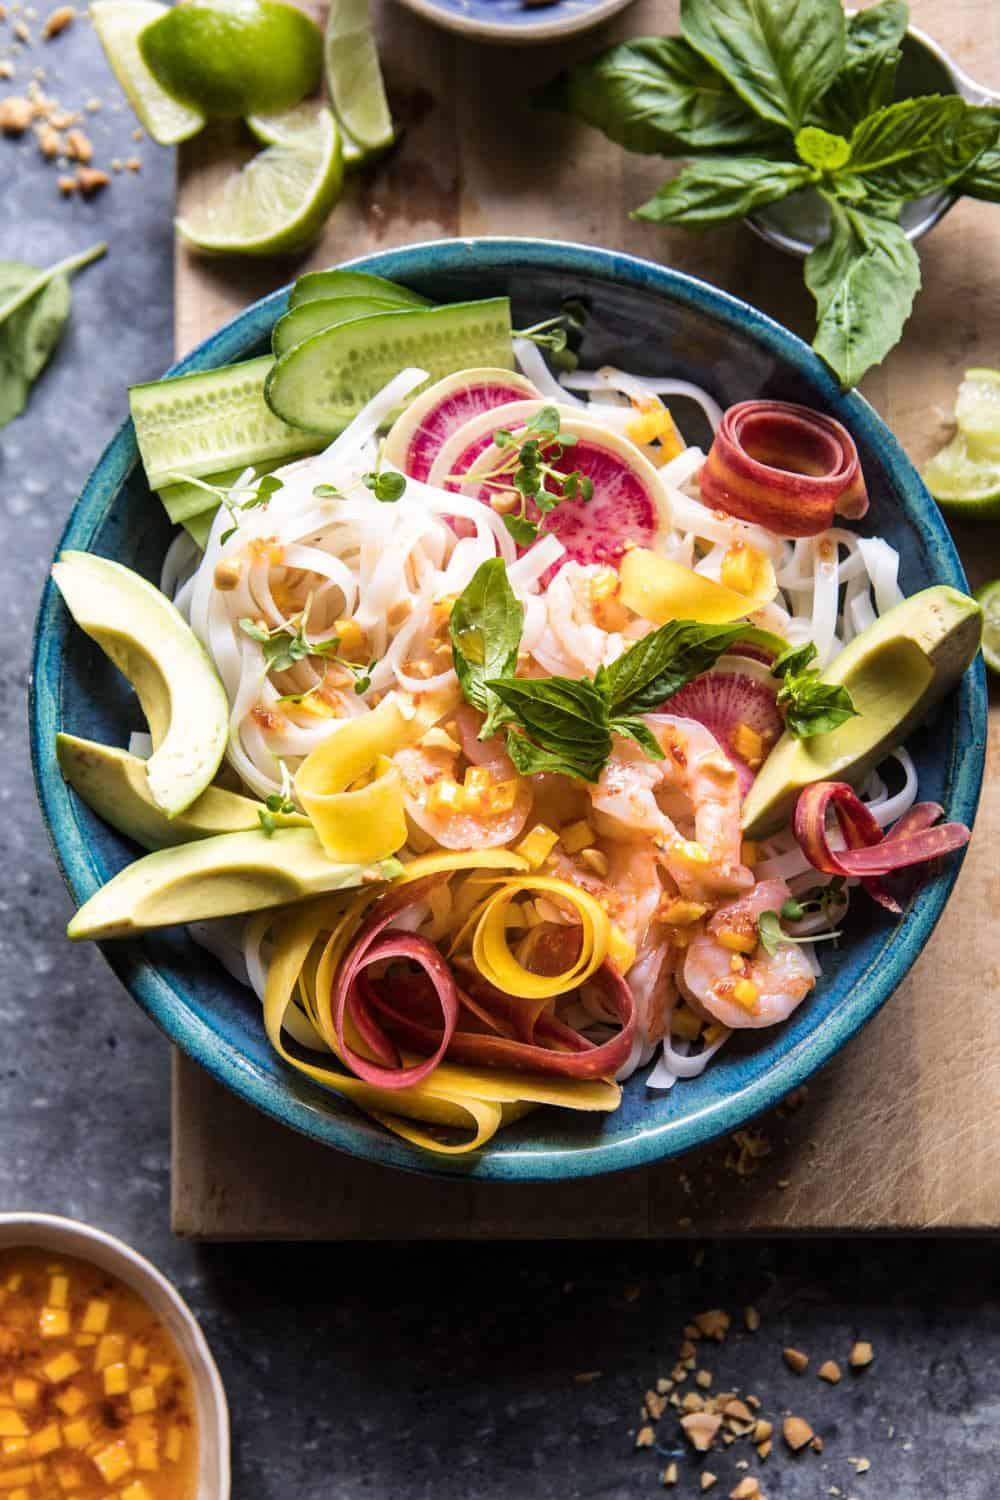
\includegraphics[width=1\textwidth,height=\textheight]{images/vietnamese-shrimp-spring-roll-bowl-with-sweet-chili-mango-sauce.jpg}

\textbf{Prep Time:} 20 min \textbar{} \textbf{Cook Time:} 5 min
\textbar{} \textbf{Total Time:} 25 min

\section{Ingredients}\label{ingredients-20}

\begin{itemize}
\tightlist
\item
  1/4 cup peanut or sesame oil
\item
  1/4 cup fresh lime juice
\item
  2 tablespoons rice vinegar
\item
  3 tablespoons honey
\item
  1-2 tablespoons fish sauce or low sodium soy sauce ((I use both))
\item
  1-2 tablespoons chili sauce ((sambal oelek))
\item
  1 inch fresh ginger, grated
\item
  1/2 ripe mango, diced
\item
  8 ounces rice noodles
\item
  1 pound cooked shrimp
\item
  4 carrots, shredded
\item
  2 radishes, thinly sliced
\item
  2 Persian cucumbers, sliced
\item
  1 bell pepper, chopped
\item
  1 avocado, sliced
\item
  1 large handful fresh basil and cilantro
\item
  1 large handful fresh basil
\item
  chopped peanuts for serving
\end{itemize}

\section{Instructions}\label{instructions-20}

\begin{enumerate}
\def\labelenumi{\arabic{enumi}.}
\tightlist
\item
\end{enumerate}

\bookmarksetup{startatroot}

\chapter{Vibrant Spring Broccoli Buddha
Bowl}\label{vibrant-spring-broccoli-buddha-bowl}

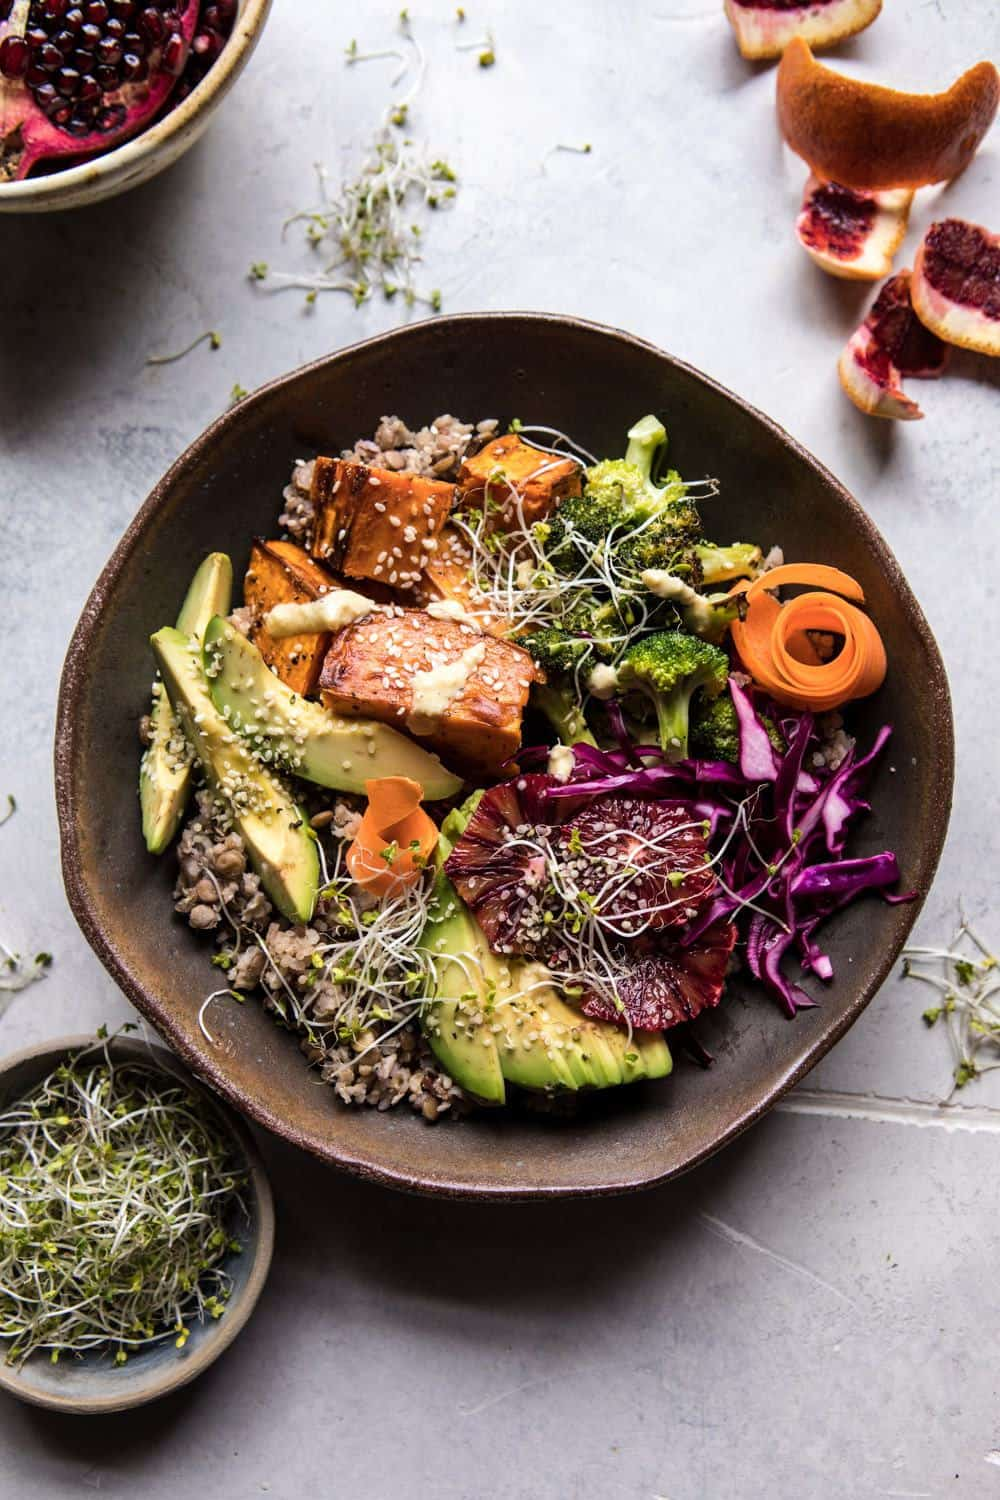
\includegraphics[width=1\textwidth,height=\textheight]{images/vibrant-spring-broccoli-buddha-bowl.jpg}

\textbf{Prep Time:} 20 min \textbar{} \textbf{Cook Time:} 30 min
\textbar{} \textbf{Total Time:} 50 min

\section{Ingredients}\label{ingredients-21}

\begin{itemize}
\tightlist
\item
  2 heads broccoli, cut into florets
\item
  1 large sweet potato, cut into wedges
\item
  2 tablespoons extra virgin olive oil
\item
  kosher salt and pepper
\item
  2 tablespoons raw sesame seeds
\item
  2 cups shredded purple cabbage
\item
  1 juice from 1 lemon
\item
  1 cup cooked quinoa or brown rice
\item
  1 cup cooked green lentils
\item
  2 carrots shredded
\item
  1 avocado sliced
\item
  1 caracara or blood orange, sliced
\item
  sprouts and hemp seeds, for serving
\item
  ½ cup roasted cashews
\item
  1-2 cloves garlic, smashed
\item
  1 inch piece fresh ginger, peeled
\item
  1 tablespoon apple cider vinegar
\item
  1 tablespoon real maple syrup
\item
  1 juice from 1 lemon
\item
  ½ teaspoon ground turmeric
\item
  kosher salt and pepper
\item
  1 pinch cayenne pepper
\end{itemize}

\section{Instructions}\label{instructions-21}

\begin{enumerate}
\def\labelenumi{\arabic{enumi}.}
\tightlist
\item
  Preheat the oven to 425 degrees F.
\item
  Place the sweet potato wedges on a large baking sheet and toss with 1
  tablespoons olive oil, and a pinch each of salt and pepper. Transfer
  to the oven and cook for 15-20 minutes, then remove from the oven. Add
  the broccoli, the remaining tablespoon of olive oil and the sesame
  seeds, toss to coat. Return to the oven and roast for another 15
  minutes or until the sweet potatoes are done to your likeness.
\item
  Meanwhile, combine the cabbage, lemon juice, and a pinch of salt in a
  medium bowl and massage with your hands for 30 seconds to 1 minute.
\item
  To assemble, toss the rice with the lentils and divide among bowls.
  Add the roasted veggies, cabbage, carrots, avocado, and oranges. Top
  with sprouts and hemp seeds and drizzle with the dressing (recipe
  follows).
\end{enumerate}

\bookmarksetup{startatroot}

\chapter{Sun-Dried Tomato and Ricotta Turkey
Meatballs}\label{sun-dried-tomato-and-ricotta-turkey-meatballs}

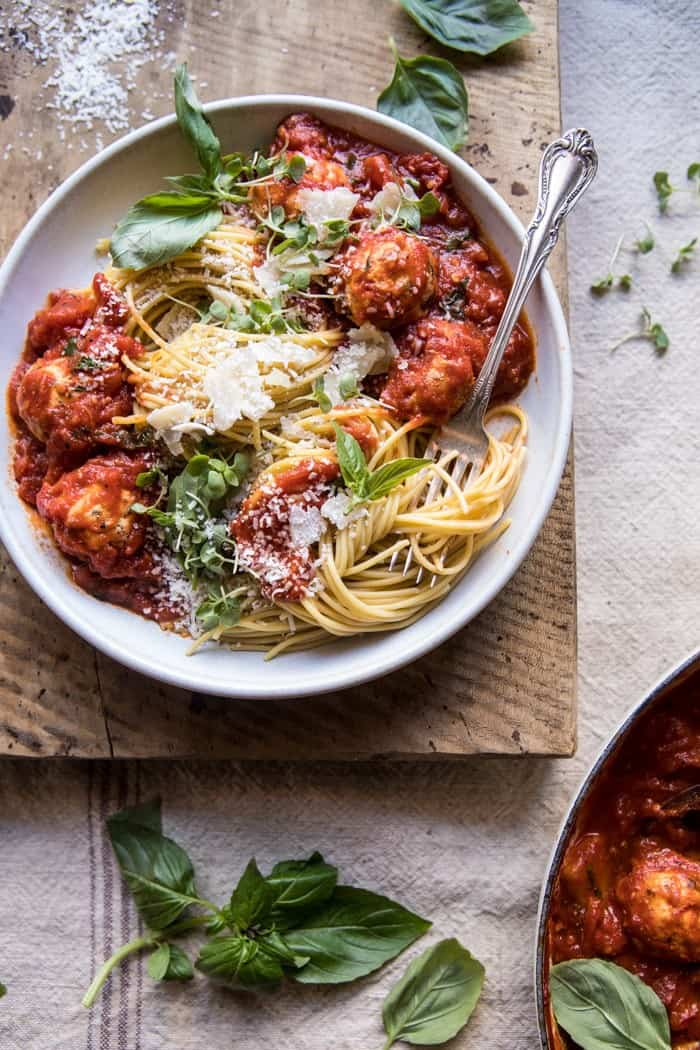
\includegraphics[width=1\textwidth,height=\textheight]{images/sun-dried-tomato-and-ricotta-turkey-meatballs.jpg}

\textbf{Prep Time:} 15 min \textbar{} \textbf{Cook Time:} 30 min
\textbar{} \textbf{Total Time:} 45 min

\section{Ingredients}\label{ingredients-22}

\begin{itemize}
\tightlist
\item
  1 pound ground turkey or chicken
\item
  3/4 cup whole milk ricotta cheese
\item
  1/4 cup grated parmesan cheese, plus more for serving
\item
  1/4 cup marinated oil packed sun-dried tomatoes, oil drained and
  chopped
\item
  3 cloves garlic, minced or grated
\item
  1 cup fresh basil, chopped
\item
  1/4 cup fresh parsley, chopped
\item
  1/2 teaspoon crushed red pepper flakes
\item
  kosher salt and black pepper
\item
  2 cans (28 ounces) San Marzano tomatoes
\item
  1/2 cup white wine
\item
  1 teaspoon dried oregano
\item
  spaghetti, for serving
\end{itemize}

\section{Instructions}\label{instructions-22}

\begin{enumerate}
\def\labelenumi{\arabic{enumi}.}
\tightlist
\item
  Preheat the oven to 450 degrees F. Line a baking sheet with parchment.
\item
  Add the turkey, ricotta, parmesan, sun-dried tomatoes, 1 clove garlic,
  1/2 cup basil, the parsley, crushed red pepper flakes, and a pinch
  each of salt and pepper to a bowl. Coat your hands with a bit of olive
  oil, and roll the meat into 2 tablespoon size balls (will make 10-12
  meatballs), placing them on the prepared baking sheet. Transfer to the
  oven and bake for 15 minutes or until the meatballs are crisp on the
  outside, but not yet cooked through on the inside.
\item
  To a large pot set over medium heat, add the tomatoes - crushing them
  by hand as you add them, the wine, remaining 2 cloves garlic, oregano,
  and a large pinch each of salt and pepper. Bring to a simmer over
  medium heat, stir in the meatballs and cook stirring occasionally,
  until the sauce thickens slightly and the meatballs are cooked
  through, about 25-30 minutes. Stir in the remaining 1/2 cup basil.
\item
  Divide the pasta among plates and spoon the meatballs and sauce over
  the pasta. Top with fresh basil.
\end{enumerate}

\bookmarksetup{startatroot}

\chapter{Sheet Pan Harissa Chicken with Chickpeas and Sweet
Potatoes}\label{sheet-pan-harissa-chicken-with-chickpeas-and-sweet-potatoes}

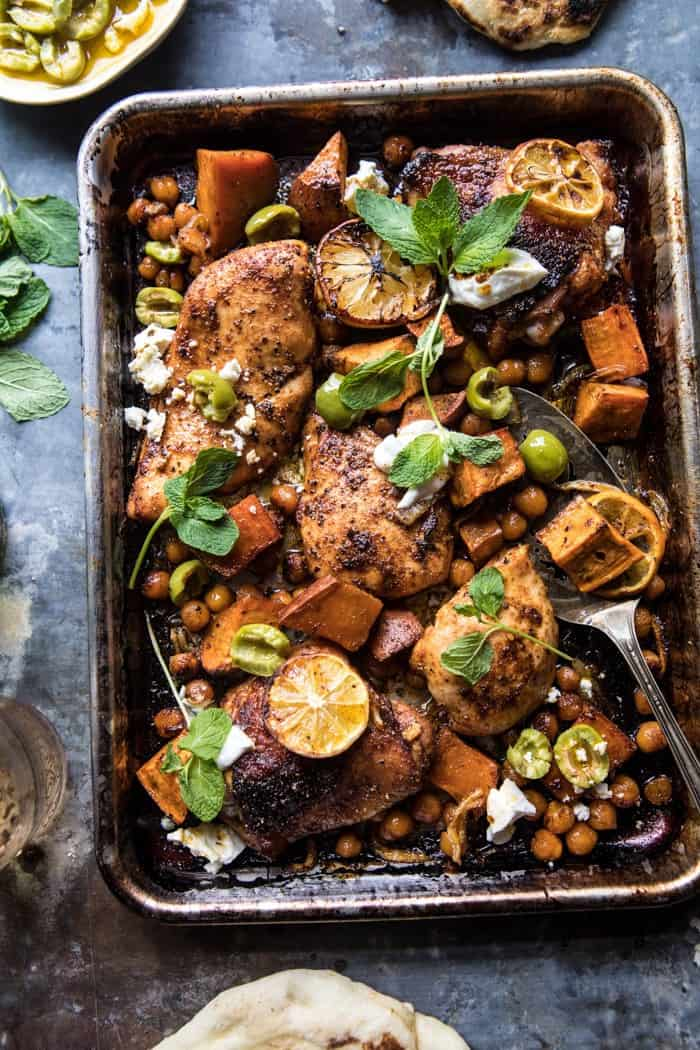
\includegraphics[width=1\textwidth,height=\textheight]{images/sheet-pan-harissa-chicken-with-chickpeas-and-sweet-potatoes.jpg}

\textbf{Prep Time:} 15 min \textbar{} \textbf{Cook Time:} 40 min
\textbar{} \textbf{Total Time:} 55 min

\section{Ingredients}\label{ingredients-23}

\begin{itemize}
\tightlist
\item
  1 1/2 pounds boneless chicken breasts or thighs
\item
  1/4 cup olive oil plus, more for drizzling
\item
  2 lemons, juice and zest from 1 + 1 sliced
\item
  2 tablespoons Harissa seasoning
\item
  1 tablespoon honey
\item
  kosher salt and black pepper
\item
  2 medium sweet potatoes, cut into 1 inch chunks
\item
  1 sweet onion, sliced
\item
  1 can (14 ounces) chickpeas, drained
\item
  1/2 cup crumbled feta
\item
  1/3 cup green olives, smashed
\item
  plain greek yogurt and fresh mint or cilantro, for serving
\end{itemize}

\section{Instructions}\label{instructions-23}

\begin{enumerate}
\def\labelenumi{\arabic{enumi}.}
\tightlist
\item
  Preheat the oven to 425 degrees F.
\item
  On a rimmed baking sheet, combine the chicken, 2 tablespoons olive
  oil, the lemon juice, lemon zest, harissa seasoning, honey, and a
  large pinch each of salt and pepper. Toss well to evenly coat the
  chicken. Add the sweet potatoes, onions, and chickpeas, and toss with
  the remaining 2 tablespoons olive oil, along with another pinch of
  salt and pepper. Arrange everything in an even layer. Add the lemon
  slices and then transfer to the oven. Roast for 40-45 minutes, tossing
  halfway through cooking until the chicken is cooked through and the
  potatoes are golden.
\item
  Meanwhile, combine the feta, olives, and a drizzle of olive oil in a
  bowl.
\item
  To serve, top the chicken with the feta, olives, and yogurt. Sprinkle
  with mint or cilantro. Enjoy!
\end{enumerate}

\bookmarksetup{startatroot}

\chapter{Meal Prep Tropical Jerk Chicken and Gingered
Broccoli}\label{meal-prep-tropical-jerk-chicken-and-gingered-broccoli}

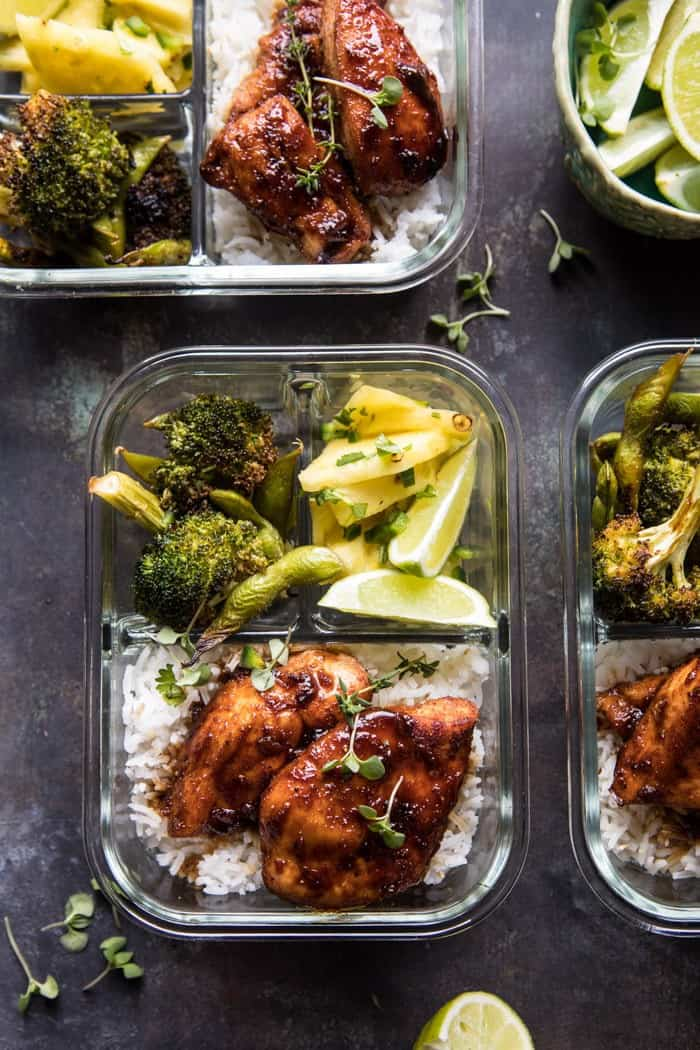
\includegraphics[width=1\textwidth,height=\textheight]{images/meal-prep-tropical-jerk-chicken-and-gingered-broccoli.jpg}

\textbf{Prep Time:} 15 min \textbar{} \textbf{Cook Time:} 25 min
\textbar{} \textbf{Total Time:} 40 min

\section{Ingredients}\label{ingredients-24}

\begin{itemize}
\tightlist
\item
  1/3 cup low sodium soy sauce
\item
  1/3 cup pineapple juice
\item
  1/3 cup honey
\item
  2 tablespoons grated fresh ginger
\item
  1 tablespoon jerk seasoning
\item
  2 tablespoons sesame oil
\item
  1 1/2 pounds boneless chicken breasts
\item
  2 heads broccoli, cut into florets
\item
  2 cups frozen edamame
\item
  4 cups coconut rice
\item
  2 cups chopped pineapple
\item
  1 jalapeño, chopped
\item
  1/4 cup fresh cilantro, chopped
\item
  juices from 1 lime or lemon
\end{itemize}

\section{Instructions}\label{instructions-24}

\begin{enumerate}
\def\labelenumi{\arabic{enumi}.}
\tightlist
\item
  Preheat the oven to 425 degrees F.
\item
  In a bowl, combine the soy sauce, pineapple juice, honey, 1 tablespoon
  ginger, 1 clove garlic, and 1 tablespoon sesame oil.
\item
  On a baking sheet, toss the chicken with the jerk seasoning and half
  of the teriyaki sauce. Slide the chicken to one side of the baking
  sheet. On the opposite side, toss the broccoli and edamame with the
  remaining 1 tablespoon ginger, and 1 tablespoon sesame oil. Season
  with salt and pepper. Transfer to the oven and roast for 15-20 minutes
  or until the chicken is cooked through and the broccoli lightly
  charred.
\item
  Meanwhile, transfer the remaining teriyaki sauce to small sauce pan
  and bring to a boil over high heat. Simmer 3-5 minutes or until the
  sauce thickens slightly.
\item
  Divide the rice among 4-6 storage containers and arrange the chicken,
  and veggies on top. Drizzle the chicken with the teriyaki sauce.
  Alternately, you can store the rice, chicken, and veggies in separate
  containers and assemble when ready. Food will keep in the fridge for
  up to 1 week.
\item
  Before serving, warm each bowl, if desired, and top with pineapple
  salsa and fresh lemon or lime juice.
\end{enumerate}

\bookmarksetup{startatroot}

\chapter{Easy Chocolate Heart
Doughnuts}\label{easy-chocolate-heart-doughnuts}


\includegraphics[width=1\textwidth,height=\textheight]{images/easy-chocolate-heart-doughnuts.jpg}

\textbf{Prep Time:} 20 min \textbar{} \textbf{Cook Time:} 30 min
\textbar{} \textbf{Total Time:} 50 min

\section{Ingredients}\label{ingredients-25}

\begin{itemize}
\tightlist
\item
  1 1/4 cups warm milk
\item
  2 1/2 teaspoons instant yeast
\item
  1 tablespoon granulated sugar, plus more for rolling
\item
  4 tablespoons unsalted butter, melted
\item
  2 eggs
\item
  4 cups all purpose flour
\item
  1 teaspoon salt
\item
  1/2 cup Nutella
\item
  1/4 cup heavy cream
\item
  1 teaspoon vanilla extract
\end{itemize}

\section{Instructions}\label{instructions-25}

\begin{enumerate}
\def\labelenumi{\arabic{enumi}.}
\tightlist
\item
  In a large mixing bowl (I like to use my stand mixer), combine the
  warm milk, yeast, butter and egg, mix a little to combine and then add
  4 cups flour and the salt. Knead the dough, using a dough hook or your
  hands, until the dough comes together and is smooth, about 3 minutes
  with a mixer, and 5-10 by hand. If the dough seems too sticky, add the
  remaining 1/4 cup flour. The dough should come together, but be
  slightly sticky to touch. Grease a large bowl and place the dough ball
  inside. Cover the bowl and let rise in a warm place until doubled in
  size, at least 30 minutes.
\item
  To fry the doughnuts, line 2 baking sheets with parchment. Lightly
  flour a work surface and roll out the dough to a 1/2-inch thickness.
  Using a heart-shaped cookie cutter, cut out the hearts. Arrange the
  doughnuts on the prepared baking sheet, leaving at least 1 inch
  between doughnuts. Cover the doughnuts loosely with plastic wrap while
  the oil heats.
\item
  In a heavy-bottomed large pot or deep fryer, heat at least 2 inches of
  oil until a deep-fry thermometer registers 350 degrees F. Working in
  batches, use a slotted metal spoon or spatula to carefully place the
  doughnuts in the hot oil. Fry, flipping once, until light golden
  brown, 1 to 2 minutes per side. When done, transfer to a wire rack to
  cool. Make sure to return the oil to 350 degrees F. between batches.
\item
  To make the glaze, mix together the Nutella, heavy cream, and vanilla
  until smooth and combined. Spoon the chocolate into a pastry bag
  fitted with a tip or just use a ziplock bag with the corner snipped
  off. Pierce the base of each cooled doughnut with the piping tube (or
  us a knife) and pipe a little filling into each doughnut. Generously
  sprinkle each doughnut sugar. Enjoy!
\end{enumerate}

\bookmarksetup{startatroot}

\chapter{Browned Butter Sugar Cookie Bars with White Chocolate
Frosting}\label{browned-butter-sugar-cookie-bars-with-white-chocolate-frosting}

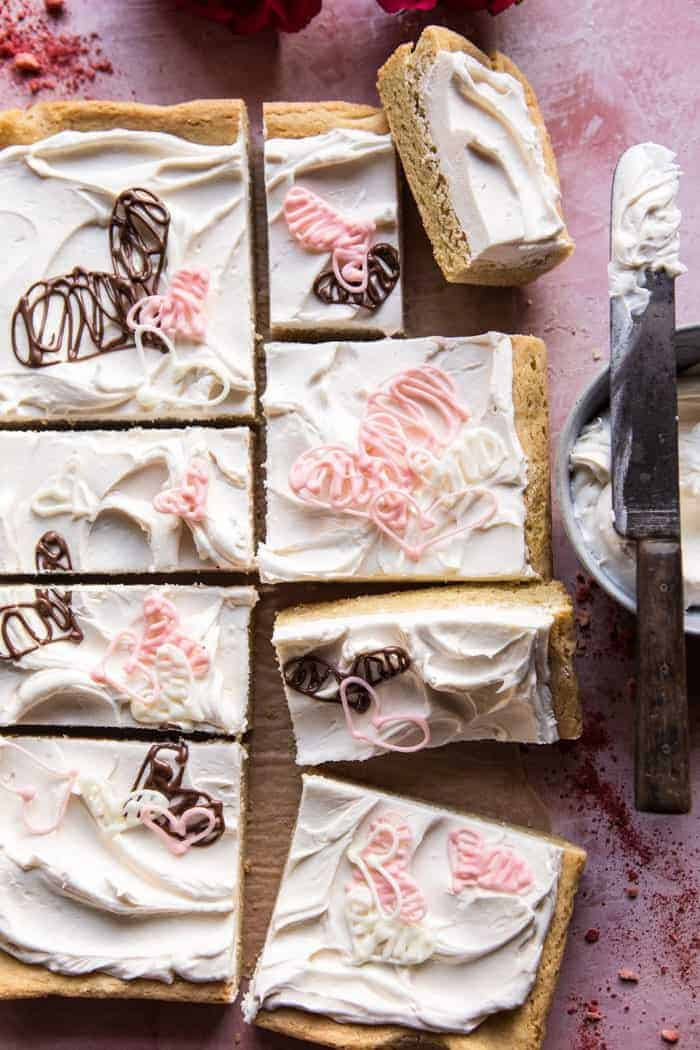
\includegraphics[width=1\textwidth,height=\textheight]{images/browned-butter-sugar-cookie-bars-with-white-chocolate-frosting.jpg}

\textbf{Prep Time:} 15 min \textbar{} \textbf{Cook Time:} 20 min
\textbar{} \textbf{Total Time:} 35 min

\section{Ingredients}\label{ingredients-26}

\begin{itemize}
\tightlist
\item
  2 sticks salted butter, cubed
\item
  1 cup granulated sugar
\item
  2 teaspoons pure vanilla extract
\item
  2 eggs, at room temperature
\item
  2 1/2 cups all-purpose flour
\item
  1 teaspoon baking soda
\item
  1 stick salted butter
\item
  1/2 cup confectioners sugar
\item
  1 cup high quality white chocolate chips, melted and cooled to touch
\item
  1 teaspoon pure vanilla extract
\item
  melted chocolate and white chocolate, for decorating
\end{itemize}

\section{Instructions}\label{instructions-26}

\begin{enumerate}
\def\labelenumi{\arabic{enumi}.}
\tightlist
\item
  Preheat the oven to 325 degrees F. Line a 9x13 inch baking pan with
  parchment paper.
\item
  Add the butter to medium pot. Allow the butter to brown lightly until
  it smells toasted, about 2-3 minutes. Stir often. Remove from the heat
  and transfer to a mixing bowl. Let cool 5 minutes. Beat in the sugar,
  and vanilla. Add the eggs, one at a time, and mix until evenly
  combined. Add the flour and baking soda, beating until combined and
  the dough forms a ball. Press the dough into the prepared baking dish.
  Transfer to the oven and bake 20 to 25 minutes or until just golden on
  top. Let cool completely before frosting.
\item
  To make the frosting: In the bowl of a stand mixer (or large bowl with
  a hand mixer) beat together the butter and powdered sugar until smooth
  and fluffy, about 5 minutes. Add the melted white chocolate, and
  vanilla, beat until combined 4. Frost the cooled cookie bars and
  decorate as desired. Cut and serve.
\end{enumerate}

\bookmarksetup{startatroot}

\chapter{Roasted Greek Chicken and Farro Salad with
Fries.}\label{roasted-greek-chicken-and-farro-salad-with-fries.}

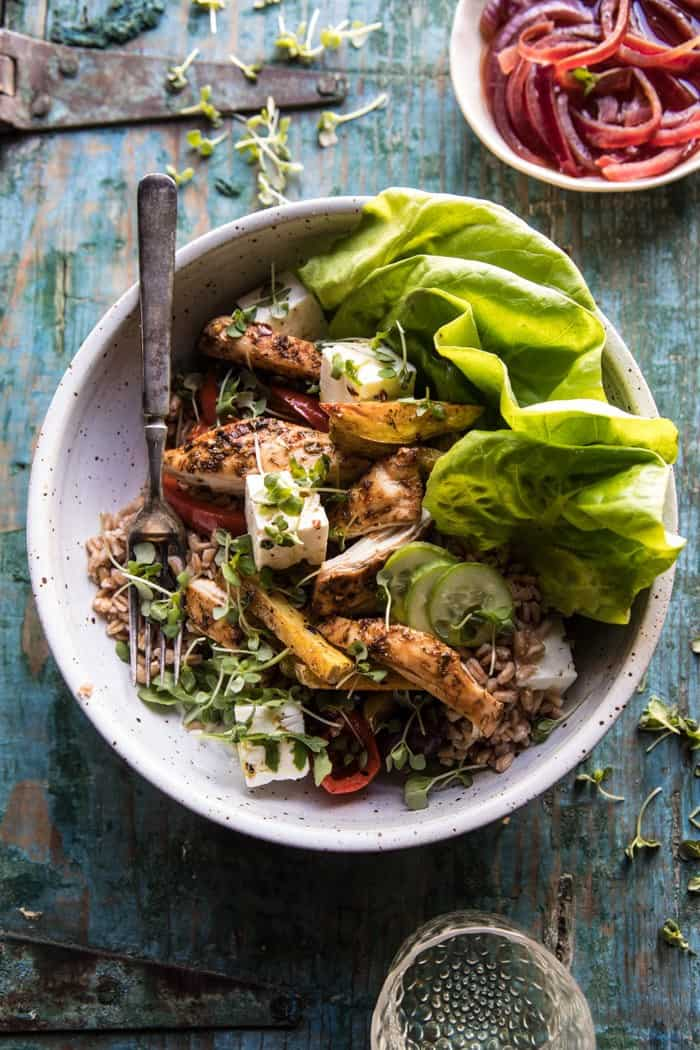
\includegraphics[width=1\textwidth,height=\textheight]{images/roasted-greek-chicken-and-farro-salad-with-fries-.jpg}

\textbf{Prep Time:} 15 min \textbar{} \textbf{Cook Time:} 40 min
\textbar{} \textbf{Total Time:} 55 min

\section{Ingredients}\label{ingredients-27}

\begin{itemize}
\tightlist
\item
  1 pound boneless chicken breasts
\item
  2 tablespoons extra virgin olive oil
\item
  2 tablespoons balsamic vinegar
\item
  1 tablespoon chopped fresh dill
\item
  1 tablespoon chopped fresh oregano
\item
  1 tablespoon paprika
\item
  2 cloves garlic, minced or grated
\item
  kosher salt and pepper
\item
  1 pound russet potatoes, cut into wedges
\item
  1-2 red bell peppers, sliced
\item
  2 cups cooked farro, or other ancient grain
\item
  1 head butter lettuce, roughly torn
\item
  8 ounces feta, cubed
\item
  tzatziki (or yogurt), olives, cucumber, red onion, for serving
\item
  1/4 cup extra virgin olive oil
\item
  3 tablespoons red wine vinegar
\item
  1 teaspoon honey
\item
  juice from 1 lemon
\item
  1 tablespoon chopped fresh oregano
\item
  1-2 cloves garlic, minced or grated
\item
  1 pinch crushed red pepper flakes
\item
  kosher salt and pepper
\end{itemize}

\section{Instructions}\label{instructions-27}

\begin{enumerate}
\def\labelenumi{\arabic{enumi}.}
\tightlist
\item
  Preheat the oven to 425 degrees F.
\item
  On a rimmed baking sheet, combine the chicken, 1 tablespoon olive oil,
  the balsamic vinegar, dill, oregano, paprika, garlic and a large pinch
  of both salt and pepper. Toss well to evenly coat the chicken. Add the
  potatoes, and bell peppers, and toss with the remaining 1 tablespoon
  olive oil and a pinch of both salt and pepper. Arrange everything in
  an even layer. Roast for 40-45 minutes, tossing halfway through
  cooking until the chicken is cooked through and the potatoes golden.
  Let the chicken cool slightly and then shred into chunks.
\item
  To assemble: smear a little tzatziki into the bottom of 4 salad bowls.
  Add the farro, lettuce, bell peppers, potatoes, and chicken. Sprinkle
  the feta and top as desired with olives, cucumber, and red onion.
  Drizzle with the red wine vinaigrette (recipe follows).
\end{enumerate}

\bookmarksetup{startatroot}

\chapter{Chewy Chocolate Chip Cookie
Granola}\label{chewy-chocolate-chip-cookie-granola}

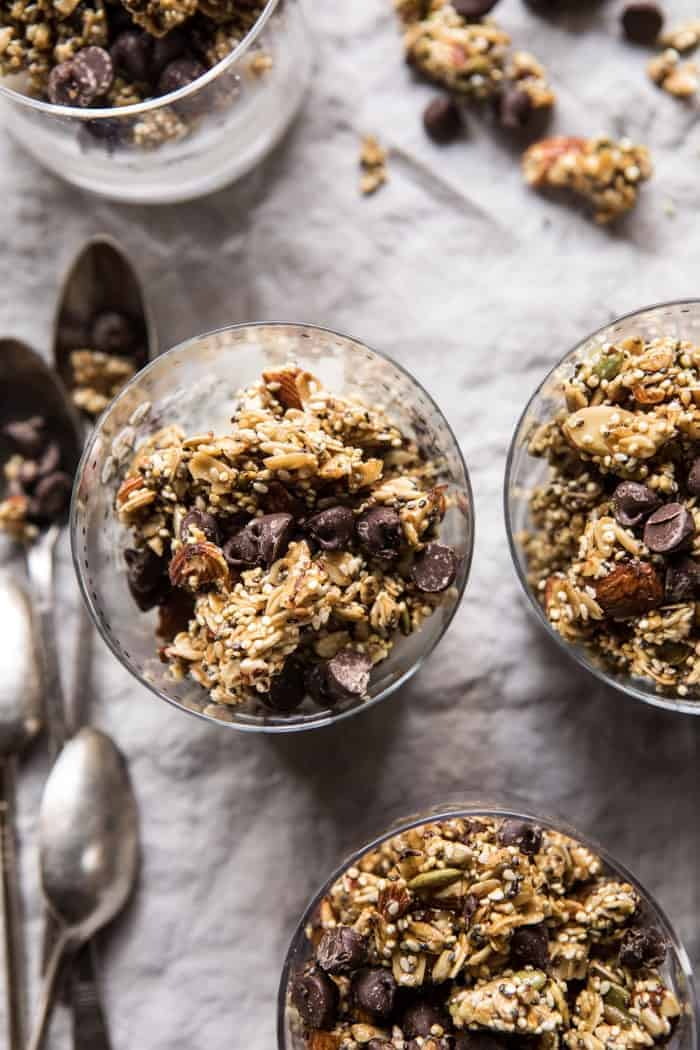
\includegraphics[width=1\textwidth,height=\textheight]{images/chewy-chocolate-chip-cookie-granola.jpg}

\textbf{Prep Time:} 15 min \textbar{} \textbf{Cook Time:} 30 min
\textbar{} \textbf{Total Time:} 45 min

\section{Ingredients}\label{ingredients-28}

\begin{itemize}
\tightlist
\item
  1 cup old fashioned oats
\item
  1/2 cup cooked quinoa
\item
  1 cup raw almonds, roughly chopped
\item
  1/2 cup raw sunflower seeds
\item
  1/4 cup raw pumpkin seeds
\item
  1/4 cup raw sesame seeds
\item
  1/4 cup chia seeds
\item
  4 tablespoons salted butter
\item
  1/2 cup + 2 tablespoons honey
\item
  2 teaspoons vanilla extract
\item
  1 cup semi-sweet or dark chocolate chips
\end{itemize}

\section{Instructions}\label{instructions-28}

\begin{enumerate}
\def\labelenumi{\arabic{enumi}.}
\tightlist
\item
  Preheat the oven to 275 degrees F. Line a baking sheet with parchment
  paper.
\item
  In a large bowl combine the oats, quinoa, almonds, sunflower seeds,
  pumpkin seeds, sesame seeds, and chia seeds.
\item
  Melt together the butter and 1/2 cup honey. Stir in the vanilla. Pour
  the mixture over the oatmeal mix and toss well to combine. Spread in
  an even layer on the prepared baking sheet. Transfer to the oven and
  bake 20 minutes. Remove from the oven, stir, and drizzle the remaining
  2 tablespoon honey over the granola. Return to the oven and bake
  another 10 -15 minutes until golden. Remove from the oven and let cool
  15-20 minutes. Stir in the chocolate chips. Keep stored in an airtight
  container for up 1 month.
\end{enumerate}

\bookmarksetup{startatroot}

\chapter{Vegan Whole Wheat Chocolate Chip Banana Bread
Muffins}\label{vegan-whole-wheat-chocolate-chip-banana-bread-muffins}

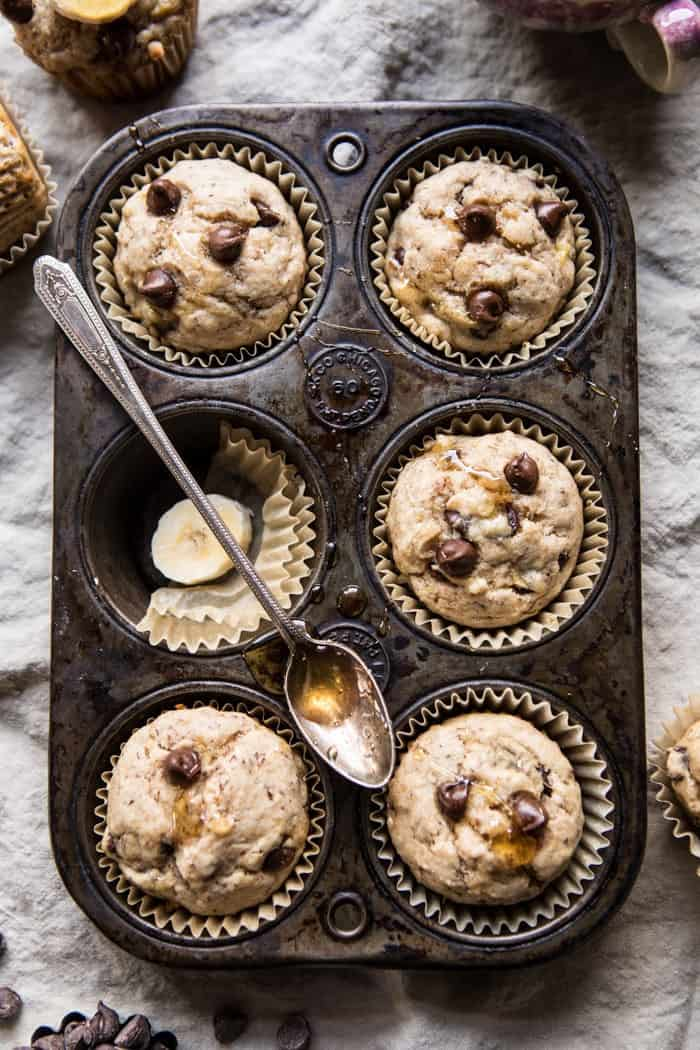
\includegraphics[width=1\textwidth,height=\textheight]{images/vegan-whole-wheat-chocolate-chip-banana-bread-muffins.jpg}

\textbf{Prep Time:} 15 min \textbar{} \textbf{Cook Time:} 20 min
\textbar{} \textbf{Total Time:} 35 min

\section{Ingredients}\label{ingredients-29}

\begin{itemize}
\tightlist
\item
  2 tablespoons ground flax meal
\item
  3 medium over-ripe bananas, mashed ((about 1 cup mashed))
\item
  1/2 cup melted coconut oil
\item
  1/2 cup real maple syrup
\item
  1/3 cup almond milk
\item
  1 tablespoon vanilla extract
\item
  2 cups white whole wheat flour
\item
  2 teaspoons baking powder
\item
  1/4 teaspoon kosher salt
\item
  1 cup dark chocolate chips
\item
  honey or maple, for serving ((optional))
\end{itemize}

\section{Instructions}\label{instructions-29}

\begin{enumerate}
\def\labelenumi{\arabic{enumi}.}
\tightlist
\item
  Preheat the oven to 350 degrees F. Line 18 muffin tins with paper
  liners.
\item
  In a small bowl, combine the ground flaxseeds with 1/3 cup water. Let
  sit 5 minutes or until thickened.
\item
  In a large mixing bowl, stir together the mashed bananas, coconut oil,
  maple syrup, almond milk, and vanilla, mix until combined. Add the
  flaxseed mixture, stirring to combine. Add the flour, baking powder,
  and salt, mix until just combined. Fold in the chocolate chips.
\item
  Divide the batter evenly among the prepared muffins tins. Transfer to
  the oven and bake for 18-20 minutes or until a toothpick inserted into
  the center comes out clean. Enjoy\ldots preferably while warm, with a
  drizzle of honey. YUM.
\end{enumerate}

\bookmarksetup{startatroot}

\chapter{Roasted Sweet Potato and Salmon Soba Noodle
Bowl}\label{roasted-sweet-potato-and-salmon-soba-noodle-bowl}

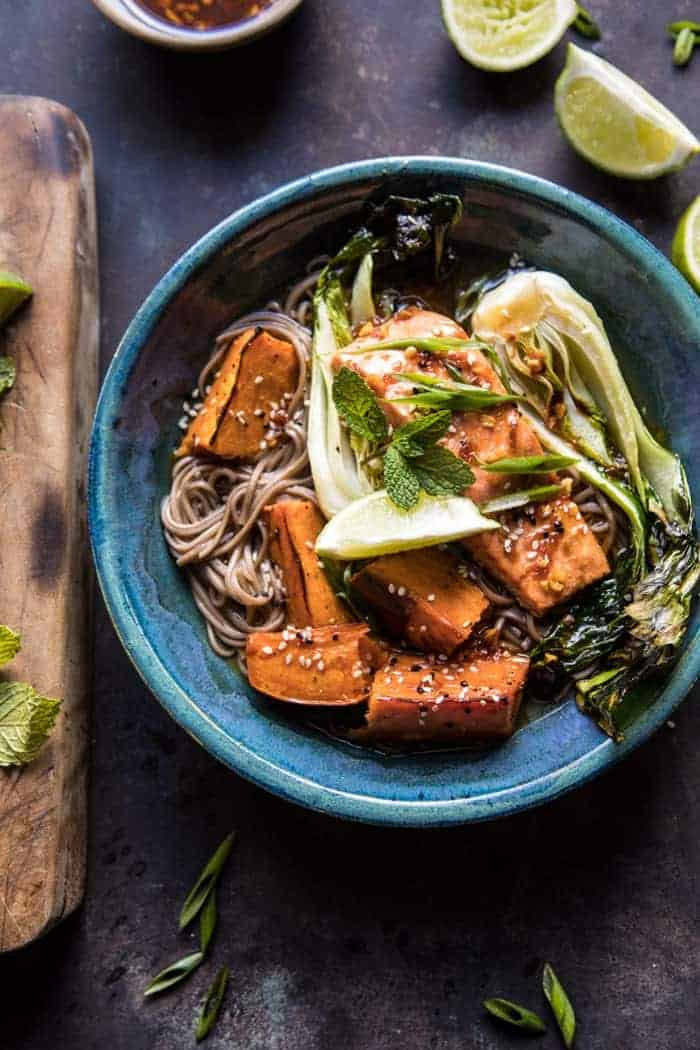
\includegraphics[width=1\textwidth,height=\textheight]{images/roasted-sweet-potato-and-salmon-soba-noodle-bowl.jpg}

\textbf{Prep Time:} 15 min \textbar{} \textbf{Cook Time:} 30 min
\textbar{} \textbf{Total Time:} 45 min

\section{Ingredients}\label{ingredients-30}

\begin{itemize}
\tightlist
\item
  2 medium sweet potato, cut into wedges
\item
  2 tablespoons extra virgin olive oil
\item
  kosher salt and pepper
\item
  3 tablespoons toasted sesame oil
\item
  1 inch fresh ginger, grated
\item
  1 clove garlic, minced or grated
\item
  juice from 1 lime
\item
  3 tablespoons low sodium soy sauce or tamari
\item
  1 tablespoon honey
\item
  2 teaspoons chili paste
\item
  4 wild caught salmon fillets
\item
  4 baby bok choy, halved
\item
  12 ounces soba noodles
\item
  4 cups low sodium chicken or veggie broth
\item
  1/4 cup rice vinegar
\item
  toasted sesame seeds, green onions, and basil for serving
\end{itemize}

\section{Instructions}\label{instructions-30}

\begin{enumerate}
\def\labelenumi{\arabic{enumi}.}
\tightlist
\item
  Preheat oven to 425 degrees F.
\item
  On a large rimmed baking sheet, combine the sweet potatoes, olive oil,
  and a pinch each of salt and pepper. Toss well to evenly coat. Place
  in the oven and roast for 20 minutes.
\item
  To make the chili sauce. Combine the sesame oil, ginger, garlic, lime
  juice, 2 tablespoons soy sauce, honey, and chili paste in a glass jar.
  Shake to combine.
\item
  Remove the sweet potatoes from the oven. Arrange the salmon and bok
  choy around the potatoes. Spoon half of the chili sauce over the
  salmon. Transfer to the oven and roast for 10-15 minutes or until the
  salmon has reached your desired doneness. Spoon the remaining chili
  sauce over the veggies and salmon, gently tossing to combine.
\item
  Meanwhile, cook the soba noodles according to package directions.
  Drain. In a pot, bring the broth, rice vinegar, and remaining
  tablespoon of soy sauce to a boil over high heat. Keep warm.
\item
  To serve, divide the noodles, roasted veggies, and salmon among bowls.
  Ladle the broth over top. Garnish with sesame seeds and herbs. Enjoy!
\end{enumerate}

\bookmarksetup{startatroot}

\chapter{The Best Everything Spice Egg Avocado Yogurt
Bowl}\label{the-best-everything-spice-egg-avocado-yogurt-bowl}

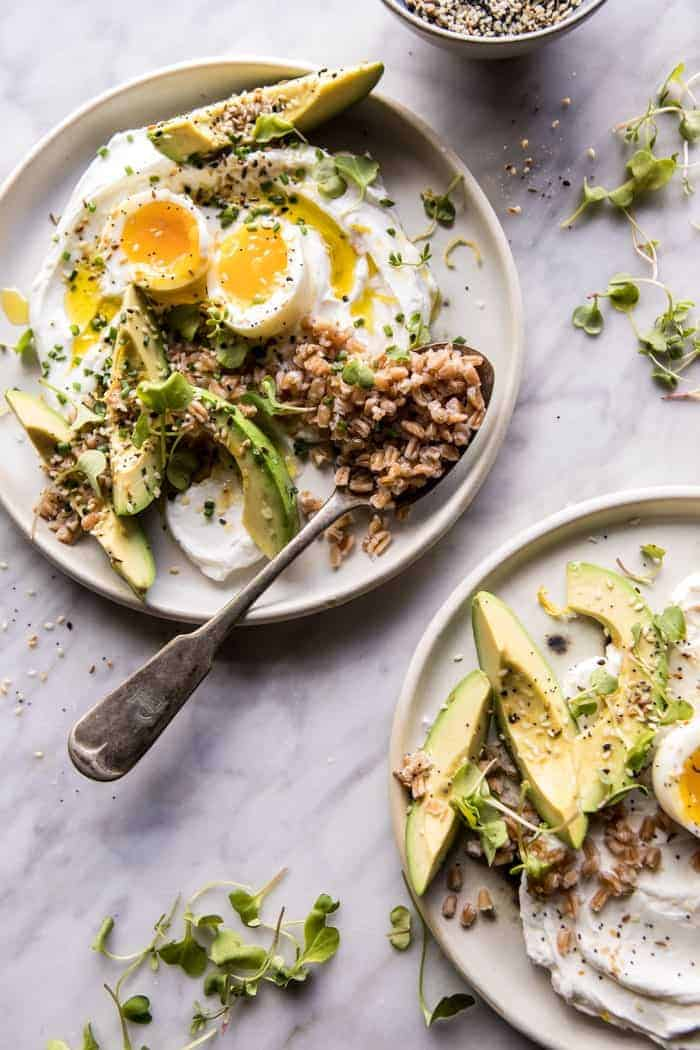
\includegraphics[width=1\textwidth,height=\textheight]{images/the-best-everything-spice-egg-avocado-yogurt-bowl.jpg}

\textbf{Prep Time:} 10 min \textbar{} \textbf{Cook Time:} 10 min
\textbar{} \textbf{Total Time:} 20 min

\section{Ingredients}\label{ingredients-31}

\begin{itemize}
\tightlist
\item
  1 cup plain full fat greek yogurt
\item
  1 cup cooked brown rice, farro, or quinoa
\item
  2 eggs, soft-boiled, poached, or fried
\item
  1 avocado, sliced
\item
  juice from 1 lemon
\item
  2 tablespoons everything bagel spice, homemade or store-bought
\item
  1 cup arugula or micro greens
\item
  flaky sea salt
\item
  extra virgin olive oil
\item
  fresh chopped chives, basil, or dill, for serving
\end{itemize}

\section{Instructions}\label{instructions-31}

\begin{enumerate}
\def\labelenumi{\arabic{enumi}.}
\tightlist
\item
  Spread the yogurt between 2 bowls. Top with brown rice, eggs, and
  avocado. Drizzle with lemon juice. Sprinkle with everything spice. Add
  a handful of greens. Drizzle each bowl lightly with olive oil and
  sprinkle with fresh herbs. Enjoy!
\end{enumerate}

\bookmarksetup{startatroot}

\chapter{Extra Fudgy Ricotta
Brownies}\label{extra-fudgy-ricotta-brownies}

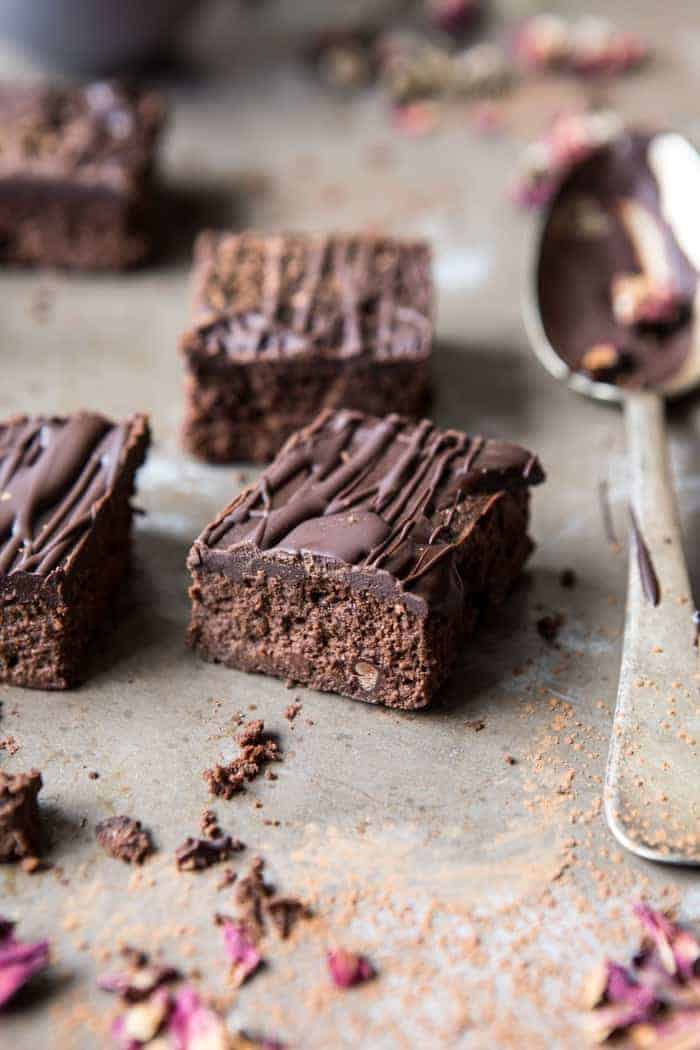
\includegraphics[width=1\textwidth,height=\textheight]{images/extra-fudgy-ricotta-brownies.jpg}

\textbf{Prep Time:} 15 min \textbar{} \textbf{Cook Time:} 30 min
\textbar{} \textbf{Total Time:} 45 min

\section{Ingredients}\label{ingredients-32}

\begin{itemize}
\tightlist
\item
  4 ounces dark chocolate, chopped
\item
  1 cup whole milk ricotta cheese
\item
  1/2 cup real maple syrup
\item
  2 teaspoons instant coffee ((optional))
\item
  2 teaspoons vanilla extract
\item
  2 eggs
\item
  1/2 cup cocoa powder
\item
  1/2 cup almond meal/flour
\item
  1/4 teaspoon kosher salt
\item
  1/3 cup real maple syrup
\item
  1/4 cup coconut oil
\item
  2 ounces dark chocolate, chopped
\item
  1/3 cup cocoa powder
\end{itemize}

\section{Instructions}\label{instructions-32}

\begin{enumerate}
\def\labelenumi{\arabic{enumi}.}
\tightlist
\item
  Preheat the oven to 350 degrees F. Line an 8x8 inch pan with parchment
  paper.
\item
  Heat 2 ounces dark chocolate in the microwave until melted and smooth.
  Stir in the ricotta, eggs, maple syrup, instant coffee, and vanilla
  until completely smooth and no clumps remain. Add the cocoa powder,
  almond meal, and salt. Stir until just combined. Stir in the remaining
  2 ounces of chopped dark chocolate.
\item
  Evenly spread the mixture into the prepared baking pan. Bake for 30-35
  minutes or until the brownies are just set. DO NOT over bake or these
  will become cakey. Allow to cool before frosting.
\item
  To make the frosting, melt together the maple syrup, coconut oil, and
  dark chocolate in a small saucepan over low heat until melted and
  smooth. Remove from the heat and stir in the cocoa power. Pour the
  frosting over the brownies and spread in an even layer. Place the
  brownies in the fridge and allow the frosting to set 30 minutes to 1
  hour. Cut into bars and store in an airtight container in a cool, dry
  place or in the fridge. Enjoy!
\end{enumerate}

\bookmarksetup{startatroot}

\chapter{Quick Cleansing Kale and Mushroom
Pho.}\label{quick-cleansing-kale-and-mushroom-pho.}

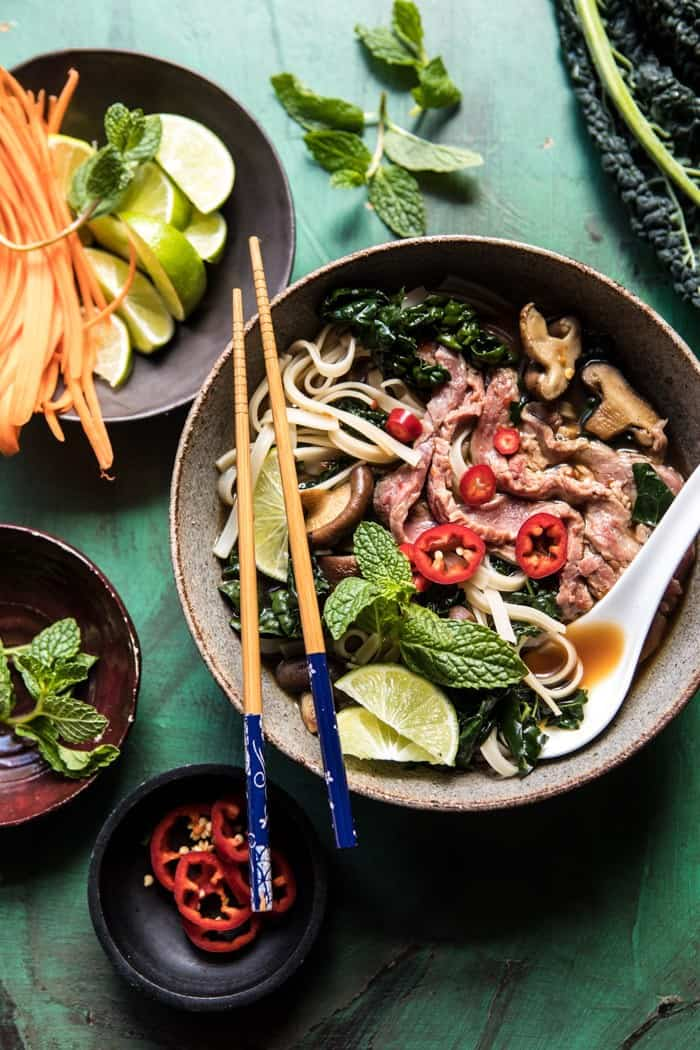
\includegraphics[width=1\textwidth,height=\textheight]{images/quick-cleansing-kale-and-mushroom-pho-.jpg}

\textbf{Prep Time:} 10 min \textbar{} \textbf{Cook Time:} 40 min
\textbar{} \textbf{Total Time:} 50 min

\section{Ingredients}\label{ingredients-33}

\begin{itemize}
\tightlist
\item
  1 tablespoon extra virgin olive oil
\item
  4 ounces shiitake mushrooms, sliced
\item
  1 onion, quartered
\item
  4 cloves garlic, smashed
\item
  1 (2-3 inch) piece ginger, sliced in half
\item
  2 star anise
\item
  2 cinnamon sticks
\item
  5 whole cloves
\item
  8 cups beef bone broth ((or beef stock))
\item
  1 tablespoon fish sauce
\item
  1 tablespoon chili paste
\item
  1 bunch Tuscan kale, roughly torn
\item
  kosher salt and pepper
\item
  4-8 ounces rice noodles
\item
  1/2 pound sirloin steak or London broil, sliced thinly ((no more than
  1/4 inch thick))
\item
  bean sprouts, mint, basil, chile peppers, green onions, carrots, and
  limes, for serving
\end{itemize}

\section{Instructions}\label{instructions-33}

\begin{enumerate}
\def\labelenumi{\arabic{enumi}.}
\tightlist
\item
  Heat the olive oil in a large soup pot over high heat. When the oil
  shimmers, add the mushrooms and a pinch of salt. Cook until the
  mushrooms are golden brown, about 4-5 minutes. Remove the mushrooms
  and set aside.
\item
  To the same pot, add the onion, garlic, and ginger and cook 3 minutes.
  Stir in the star anise, cinnamon, and cloves. Toast, stirring
  occasionally until the spices are fragrant, about 2-3 more minutes.
  Add the bone broth, fish sauce, and chili paste. Simmer for 15-20
  minutes. Remove the onion, garlic, and spices from the broth, and
  discard.
\item
  Bring the broth to a boil. Add the kale and stir in the mushrooms.
  Season to taste with salt and pepper. Simmer 10 minutes or until ready
  to serve 3. Meanwhile, bring a large pot of water to a boil and cook
  the rice noodles according to package directions.
\item
  Divide the noodles between bowls and top with thinly sliced steak.
  Ladle the hot broth over the steak, submerging the steak and noodles
  in the hot broth. Top as desired with sprouts, chilies, herbs, limes,
  onions, and carrots. Enjoy!
\end{enumerate}

\bookmarksetup{startatroot}

\chapter{Pineapple Margarita
Sparklers}\label{pineapple-margarita-sparklers}

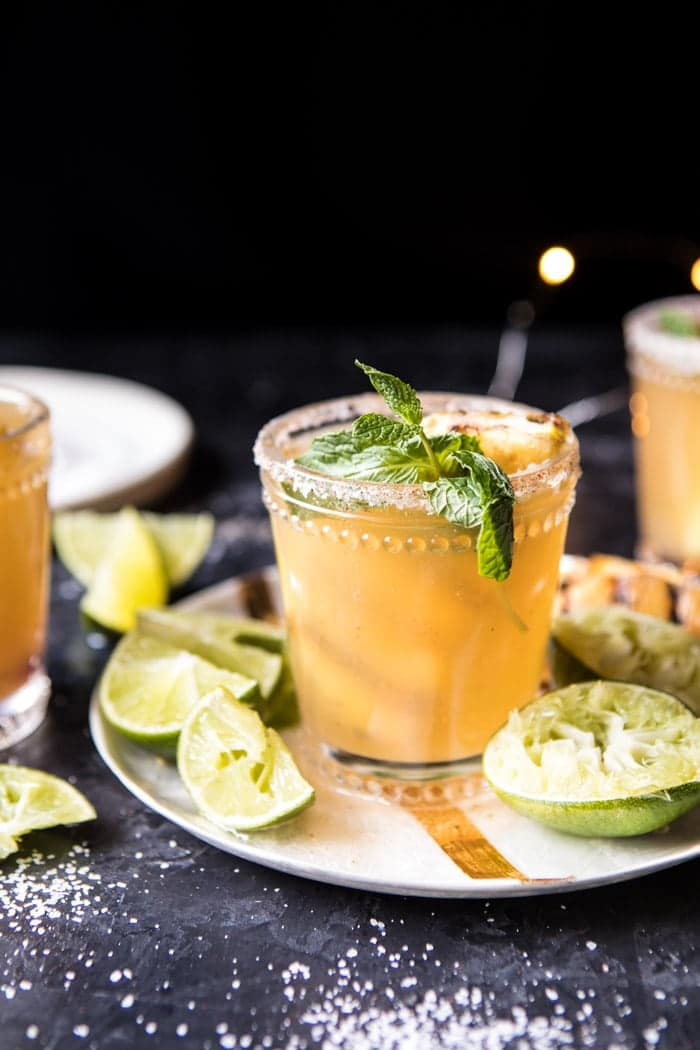
\includegraphics[width=1\textwidth,height=\textheight]{images/pineapple-margarita-sparklers.jpg}

\textbf{Prep Time:} 10 min \textbar{} \textbf{Cook Time:} \textbar{}
\textbf{Total Time:} 10 min

\section{Ingredients}\label{ingredients-34}

\begin{itemize}
\tightlist
\item
  1 cup fresh pineapple chunks
\item
  1 cup fresh lime juice
\item
  1/4 cup fresh lemon juice
\item
  1 cup silver tequila
\item
  1/2 cup Grand Marnier ((orange liqueur))
\item
  1 bottle (750 ml) champagne
\item
  fresh mint, for serving
\item
  1/4 cup kosher or margarita salt
\item
  1 teaspoon chipotle chili powder
\end{itemize}

\section{Instructions}\label{instructions-34}

\begin{enumerate}
\def\labelenumi{\arabic{enumi}.}
\tightlist
\item
  In a blender, combine the pineapple, lime juice, and lemon juice and
  pulse to combine. Strain into a pitcher. Add the tequila and Grand
  Marnier. Chill until ready to serve.
\item
  Just before serving, add the champagne. Rim glasses with chili salt
  and divide the margaritas among glasses. Top with fresh or grilled
  pineapple slices and mint. Enjoy!
\end{enumerate}

\bookmarksetup{startatroot}

\chapter{Seared Scallop Ravioli with Rosemary Butter and Lemon
Sauce}\label{seared-scallop-ravioli-with-rosemary-butter-and-lemon-sauce}

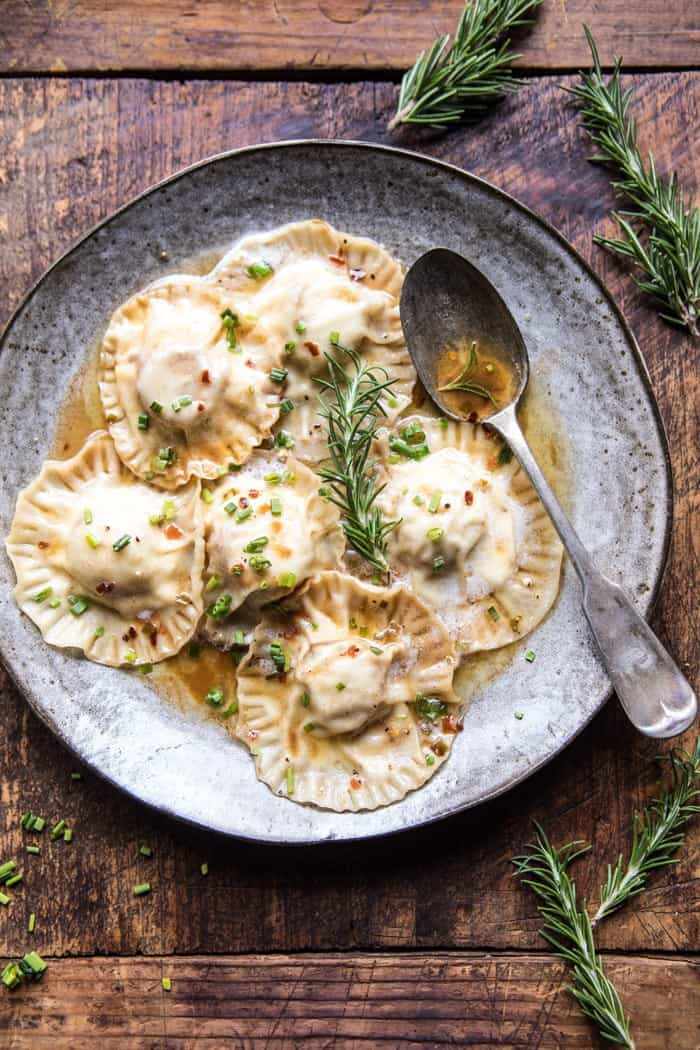
\includegraphics[width=1\textwidth,height=\textheight]{images/seared-scallop-ravioli-with-rosemary-butter-and-lemon-sauce.jpg}

\textbf{Prep Time:} 30 min \textbar{} \textbf{Cook Time:} 20 min
\textbar{} \textbf{Total Time:} 50 min

\section{Ingredients}\label{ingredients-35}

\begin{itemize}
\tightlist
\item
  1 cup whole milk ricotta cheese
\item
  1/2 cup grated manchego cheese
\item
  kosher salt and pepper
\item
  24 small wild caught scallops
\item
  2 tablespoons extra virgin olive oil
\item
  48 circle or square wonton wrappers
\item
  6 tablespoons salted butter
\item
  1 tablespoon chopped fresh rosemary plus more for serving
\item
  2 cloves garlic, minced or grated
\item
  1/4 cup white wine or chicken broth
\item
  1/4 cup fresh lemon juice
\item
  pinch of crushed red pepper flakes
\item
  kosher salt and pepper
\item
  1 tablespoon chopped fresh chives
\end{itemize}

\section{Instructions}\label{instructions-35}

\begin{enumerate}
\def\labelenumi{\arabic{enumi}.}
\tightlist
\item
  In a medium bowl, stir together the ricotta and manchego. Season with
  salt and pepper.
\item
  Heat a large skillet over medium heat. Season the scallops with salt
  and pepper. Add the olive oil to the skillet and when the oil
  shimmers, add the scallops and sear on both sides until browned, about
  2-3 minutes. Remove the scallops from the skillet to a plate. Let
  cool.
\item
  Lay out about 6 wrappers. Place 1 scallop on each wrapper and then
  spoon 1-2 teaspoons of ricotta over the scallop. Brush the edges with
  water. Lay a second wrapper on top of each ravioli. Press down the
  edges to seal, pressing out all the air. Crimp the edges with a fork.
  Be sure to keep the ravioli covered as you work to prevent them from
  drying out.
\item
  Return the skillet used to cook the scallops to medium high heat.
  Brown the butter, stirring often until the butter is golden and
  toasted. Add the rosemary and garlic and cook 30 seconds to a minute
  or until fragrant. Pour in the wine and lemon juice and bring to a
  boil. Add the chili flakes and season with salt and pepper. Cook 3-5
  minutes. Remove from the heat and add the chives.
\item
  Meanwhile, bring a large pot of salted water to a boil. Boil the
  ravioli in batches for 1-2 minutes or until they float. Drain. Be
  gentle when working with the ravioli as they are delicate.
\item
  Divide the ravioli among bowls and ladle the sauce overtop. Top with
  chives. EAT!
\end{enumerate}

\bookmarksetup{startatroot}

\chapter{Eggnog Frosted Chai Snickerdoodle
Snowmen}\label{eggnog-frosted-chai-snickerdoodle-snowmen}


\includegraphics[width=1\textwidth,height=\textheight]{images/eggnog-frosted-chai-snickerdoodle-snowmen.jpg}

\textbf{Prep Time:} 20 min \textbar{} \textbf{Cook Time:} 10 min
\textbar{} \textbf{Total Time:} 30 min

\section{Ingredients}\label{ingredients-36}

\begin{itemize}
\tightlist
\item
  2 3/4 cups all-purpose flour
\item
  1 teaspoon baking soda
\item
  1/4 teaspoon baking powder
\item
  2 sticks (1 cup) salted butter, at room temperature
\item
  4 ounces cream cheese, at room temperature
\item
  1 cup granulated sugar
\item
  1 egg
\item
  2 teaspoons vanilla extract
\item
  Mini Reese's, mini chocolate chips, sprinkles, and melted chocolate,
  for decorating
\item
  1/2 cup granulated sugar
\item
  2 teaspoons cinnamon
\item
  1/2 teaspoon ground ginger
\item
  1/2 teaspoon all-spice
\item
  1/2 teaspoon cardamom
\item
  1 stick (1/2 cup) salted butter
\item
  2 1/4 cups powdered sugar
\item
  2-4 tablespoons eggnog
\item
  1/4 teaspoon nutmeg
\end{itemize}

\section{Instructions}\label{instructions-36}

\begin{enumerate}
\def\labelenumi{\arabic{enumi}.}
\tightlist
\item
  Preheat the oven to 375 degrees F. Line 2 baking sheets with parchment
  paper.
\item
  In a medium bowl, combine the flour, baking soda, and baking powder.
\item
  Using an electric mixer, in a large bowl beat together the butter,
  cream cheese, and sugar until light and fluffy, about 2 minutes. Add
  the egg and vanilla and beat until combined. Gradually add the flour
  mixture, mixing until just fully combined.
\item
  To make the chai spice sugar. In a small bowl, combine the sugar,
  cinnamon, ginger, all-spice, and cardamom.
\item
  Roll the dough into two sizes of balls. 16 (1 1/2 inch, about 1
  tablespoon) size balls, and 16 (3/4 inch, about 2 teaspoons) size
  balls. Then generously roll through the chai sugar.
\item
  To make the snowmen, place 1 smaller baller and 1 larger ball together
  with the edges touching on the prepared baking sheet, spacing the
  cookies 2 inches apart. Repeat with the remaining dough balls.
  Transfer to the oven and bake for 8-10 minutes or until the cookies
  are just starting to set around the edges. Let cool completely.
\item
  To make the frosting, beat together the butter and sugar until creamy.
  Add the eggnog and nutmeg, beat to combine.
\item
  To frost the cooled cookies. Place half a mini Reese's atop the
  snowman's head. Decorate as desired with candies and melted chocolate.
\end{enumerate}

\bookmarksetup{startatroot}

\chapter{Cheesy Hasselback Potato Au
Gratin}\label{cheesy-hasselback-potato-au-gratin}

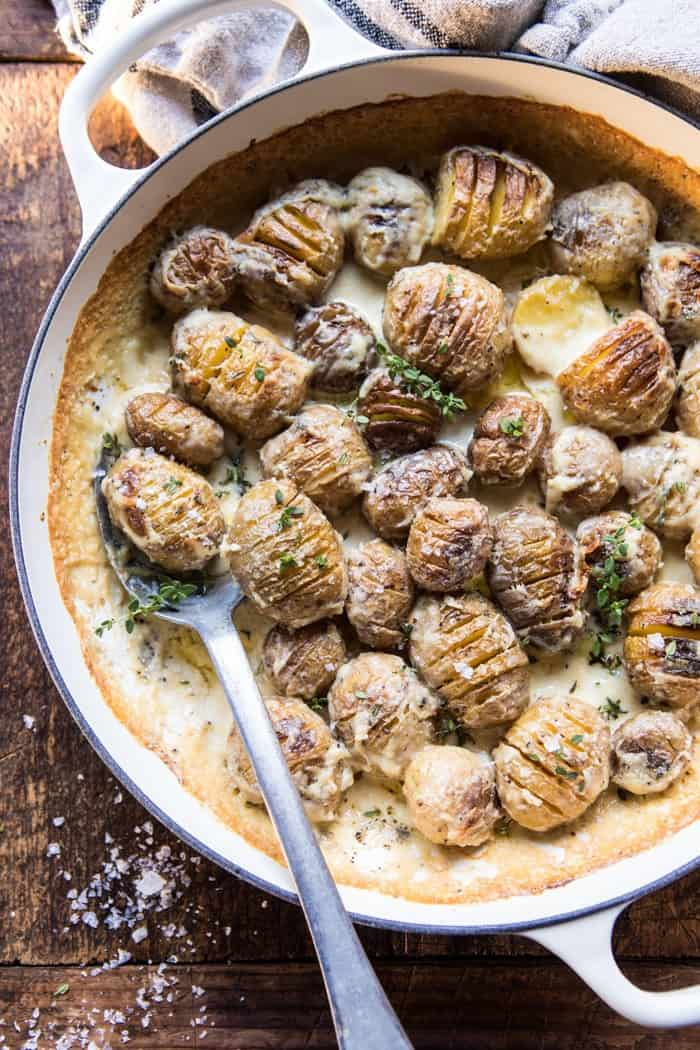
\includegraphics[width=1\textwidth,height=\textheight]{images/cheesy-hasselback-potato-au-gratin.jpg}

\textbf{Prep Time:} 15 min \textbar{} \textbf{Cook Time:} 1 hr
\textbar{} \textbf{Total Time:} 1 hr 15 min

\section{Ingredients}\label{ingredients-37}

\begin{itemize}
\tightlist
\item
  3 pounds baby potatoes, I like using a medium size
\item
  2 tablespoons extra virgin olive oil
\item
  2 cups heavy cream or whole milk
\item
  2 cloves garlic, minced or grated
\item
  1/2 cup grated manchego cheese
\item
  1/2 cup grated gruyere cheese
\item
  1 tablespoon chopped fresh thyme
\item
  2 tablespoons butter, thinly sliced
\item
  kosher salt and pepper
\end{itemize}

\section{Instructions}\label{instructions-37}

\begin{enumerate}
\def\labelenumi{\arabic{enumi}.}
\tightlist
\item
  Preheat the oven to 425 degrees F.
\item
  Carefully slice the potatoes into thin slices, leaving a 1/8 inch at
  the bottom, be careful not to slice all the way through the potato.
  Place In a 9x13 inch baking dish and gently toss with olive oil, salt,
  and pepper. Transfer to the oven and roast for 20-25 minutes.
\item
  Meanwhile, in a medium bowl, combine the cream, garlic, cheese, thyme,
  and a pinch each of salt and pepper.
\item
  Remove the potatoes from the oven and pour the cream over them,
  arrange the potatoes in a mostly even layer. Place the slices of
  butter around the potatoes. Return to the oven and roast for another
  20-25 minutes, until the sauce thickens and the potatoes are tender.
  Season with flaky salt just before serving. Enjoy!
\end{enumerate}

\bookmarksetup{startatroot}

\chapter{Homemade Cheddar Pierogies}\label{homemade-cheddar-pierogies}

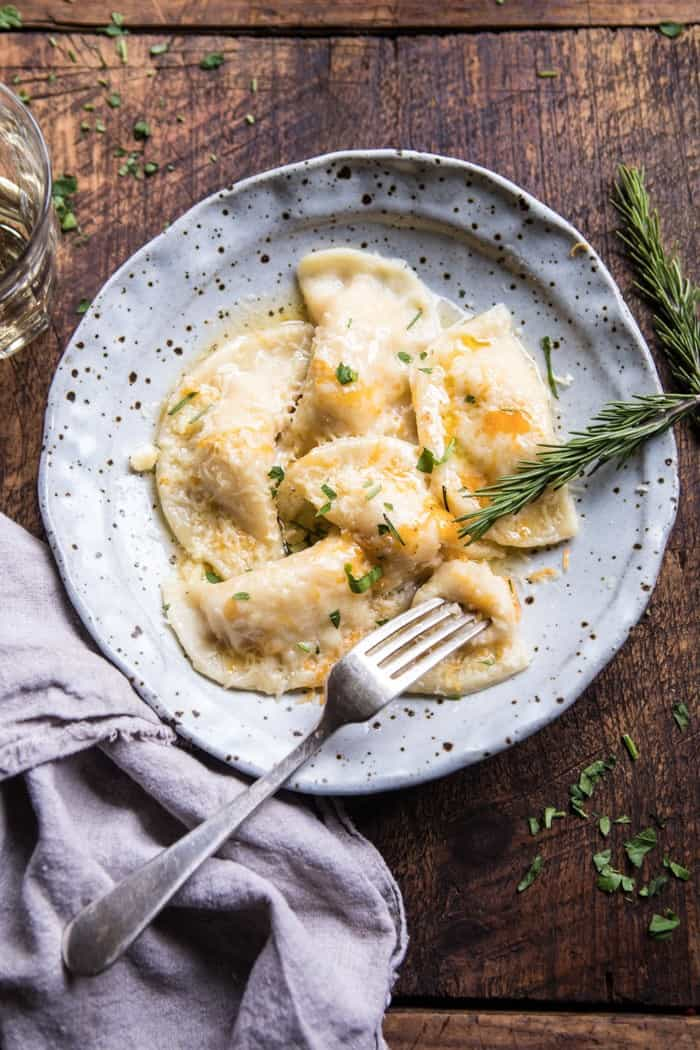
\includegraphics[width=1\textwidth,height=\textheight]{images/homemade-cheddar-pierogies.jpg}

\textbf{Prep Time:} 1 hr \textbar{} \textbf{Cook Time:} 30 min
\textbar{} \textbf{Total Time:} 1 hr 30 min

\section{Ingredients}\label{ingredients-38}

\begin{itemize}
\tightlist
\item
  2 cups all-purpose flour
\item
  1 teaspoon kosher salt
\item
  2 tablespoons butter, melted
\item
  1 cup plain full fat greek yogurt
\item
  1 egg
\item
  4 russet potatoes, peeled and quartered
\item
  2 cups shredded sharp cheddar cheese, plus more for topping
\item
  2 tablespoons butter, at room temperature
\item
  1/2 teaspoon onion powder
\item
  kosher salt and pepper
\item
  1 stick butter
\item
  1-2 cloves garlic, minced or grated ((to your taste))
\item
  1 tablespoon chopped fresh rosemary
\end{itemize}

\section{Instructions}\label{instructions-38}

\begin{enumerate}
\def\labelenumi{\arabic{enumi}.}
\tightlist
\item
  To make the dough. In a medium bowl, combine the flour, salt, butter,
  yogurt, and egg, and mix until combined. Knead the dough for 2-3
  minutes. Cover and let sit 30 minutes.
\item
  To make the filling. In a large pot of cold water, bring the potatoes
  to a boil. Salt the water and cook until the potatoes are tender,
  about 20 to 30 minutes.
\item
  Drain the potatoes, return the potatoes to the pot and mash over low
  heat, or mash in the bowl of a stand mixer fitted with the paddle
  attachment, adding the butter and cheddar cheese. Season to taste with
  salt and pepper.
\item
  Roll the dough out onto a floured surface to 1/8 inch thickness. Using
  a biscuit cutter, cut out 3-inch circles. Spoon 2 teaspoons of filling
  into the center of each round. Brush the edges with water and fold
  half of the dough over the filling to enclose it. Press down the edges
  to seal, pressing out all the air. Be sure to keep the dough covered
  as you work work to prevent from drying out. At this point, the
  Pierogies can be flash frozen on a baking sheet for 30 minutes, then
  transferred to a freezer bag and frozen for up to 3 months.
\item
  When ready too cook, bring a large pot of salted water to a boil. Boil
  the Pierogies in batches for 1-2 minutes, or until they float. Drain.
\item
  To make the butter sauce. In a large skillet, brown the butter over
  medium heat, stirring often until the butter is golden and toasted.
  Add the rosemary and garlic and cook 30 seconds to a minute or until
  fragrant. Remove from the heat. Season with salt and pepper.
\item
  Divide the Pierogies among plates and spoon the butter over the
  Pierogies. Top with cheddar and parsley. EAT!
\end{enumerate}

\bookmarksetup{startatroot}

\chapter{Buddy the Elf Cocktail}\label{buddy-the-elf-cocktail}


\includegraphics[width=1\textwidth,height=\textheight]{images/buddy-the-elf-cocktail.jpg}

\textbf{Prep Time:} 10 min \textbar{} \textbf{Cook Time:} \textbar{}
\textbf{Total Time:} 10 min

\section{Ingredients}\label{ingredients-39}

\begin{itemize}
\tightlist
\item
  4 ounces (1/2 cup) vodka
\item
  2 ounces (1/4 cup) Kahlúa, or more to taste
\item
  3 tablespoons maple syrup
\item
  2 teaspoon vanilla extract
\item
  3 teaspoons molasses
\item
  1/4 teaspoon ground cinnamon
\item
  1/8 teaspoon ginger
\item
  1/2 cup heavy cream, whole milk, or sweetened condensed milk
\item
  chocolate syrup, for topping
\item
  whipped cream, candy canes, candies, and gingerbread cookies, for
  serving
\end{itemize}

\section{Instructions}\label{instructions-39}

\begin{enumerate}
\def\labelenumi{\arabic{enumi}.}
\tightlist
\item
  In a cocktail shaker combine the vodka, Kahlúa, maple syrup, vanilla,
  molasses, cinnamon, and ginger. Shake until well combined. Add ice and
  shake again. Strain into 4 glasses. Top off each glass with heavy
  cream, whole milk or sweetened condensed milk. Dollop with whipped
  cream and garnish as desired. DRINK!
\end{enumerate}

\bookmarksetup{startatroot}

\chapter{Lemony Fried Brussels
Sprouts}\label{lemony-fried-brussels-sprouts}

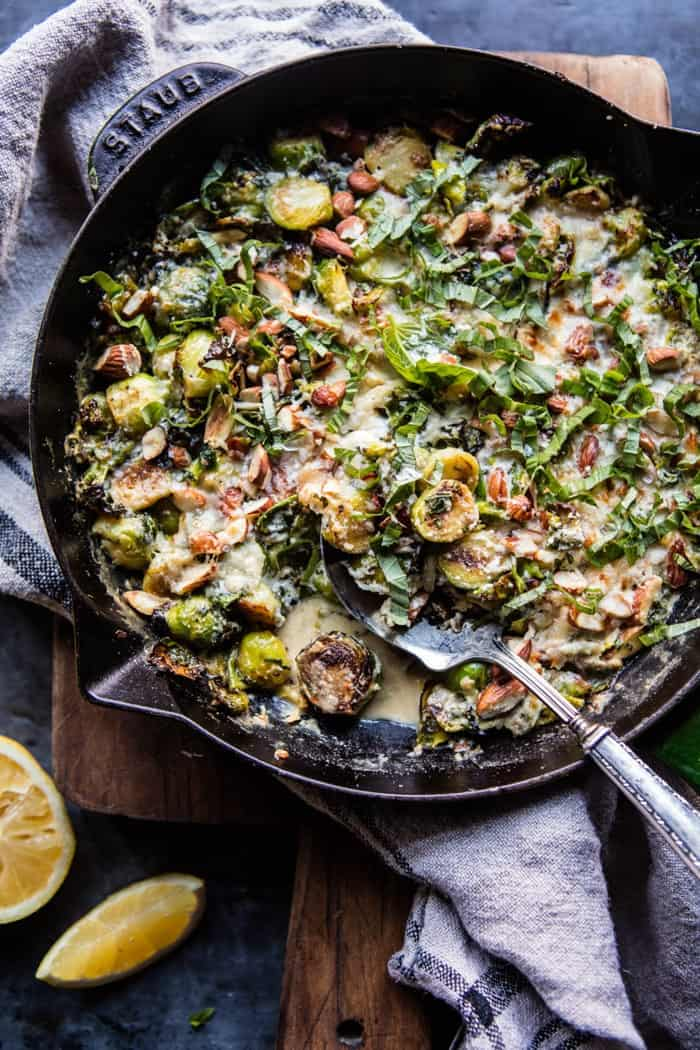
\includegraphics[width=1\textwidth,height=\textheight]{images/lemony-fried-brussels-sprouts.jpg}

\textbf{Prep Time:} 10 min \textbar{} \textbf{Cook Time:} 20 min
\textbar{} \textbf{Total Time:} 30 min

\section{Ingredients}\label{ingredients-40}

\begin{itemize}
\tightlist
\item
  2 tablespoons extra-virgin olive oil
\item
  ¾ pound Brussels sprouts, trimmed and halved
\item
  4 garlic cloves, minced or grated
\item
  Zest of 1 lemon
\item
  ⅔ cup full-fat goat’s milk
\item
  2 ounces goat cheese
\item
  1 teaspoon Dijon mustard
\item
  1 tablespoon fresh lemon juice
\item
  Pinch of crushed red pepper flakes
\item
  ¼ cup chopped fresh basil, plus more for garnish
\item
  ⅓ cup grated Parmesan cheese
\item
  ⅓ cup raw almonds, coarsely chopped
\item
  Flaky sea salt and freshly ground black pepper
\end{itemize}

\section{Instructions}\label{instructions-40}

\begin{enumerate}
\def\labelenumi{\arabic{enumi}.}
\tightlist
\item
  Preheat the oven to 400ºF.
\item
  In a 12-inch oven-safe skillet, heat the olive oil over medium. When
  it shimmers, add the Brussels sprouts and cook, stirring occasionally,
  until crisp and lightly caramelized, 3 to 4 minutes. Add the garlic
  and lemon zest and cook until fragrant, about 30 seconds, being sure
  not to burn them.
\item
  Transfer the skillet to the oven and roast the Brussels sprouts for
  about 10 minutes, or until tender.
\item
  Meanwhile, in a blender or food processor, combine the goat’s milk,
  goat cheese, mustard, and lemon juice and pulse until smooth. Stir in
  the red pepper flakes.
\item
  Remove the Brussels sprouts from the oven. Turn the broiler to high.
  Stir the basil and mint into the Brussels sprouts. Pour the goat’s
  milk mixture on top. Sprinkle with the Parmesan and almonds. Return to
  the oven and broil for 2 to 3 minutes, or until the cheese has melted,
  keeping a close eye on it. Remove and season lightly with flaky sea
  salt and pepper. Garnish with fresh basil and mint.
\end{enumerate}

\bookmarksetup{startatroot}

\chapter{The Cheese-Maker’s Mac and
Cheese}\label{the-cheese-makeruxe2s-mac-and-cheese}

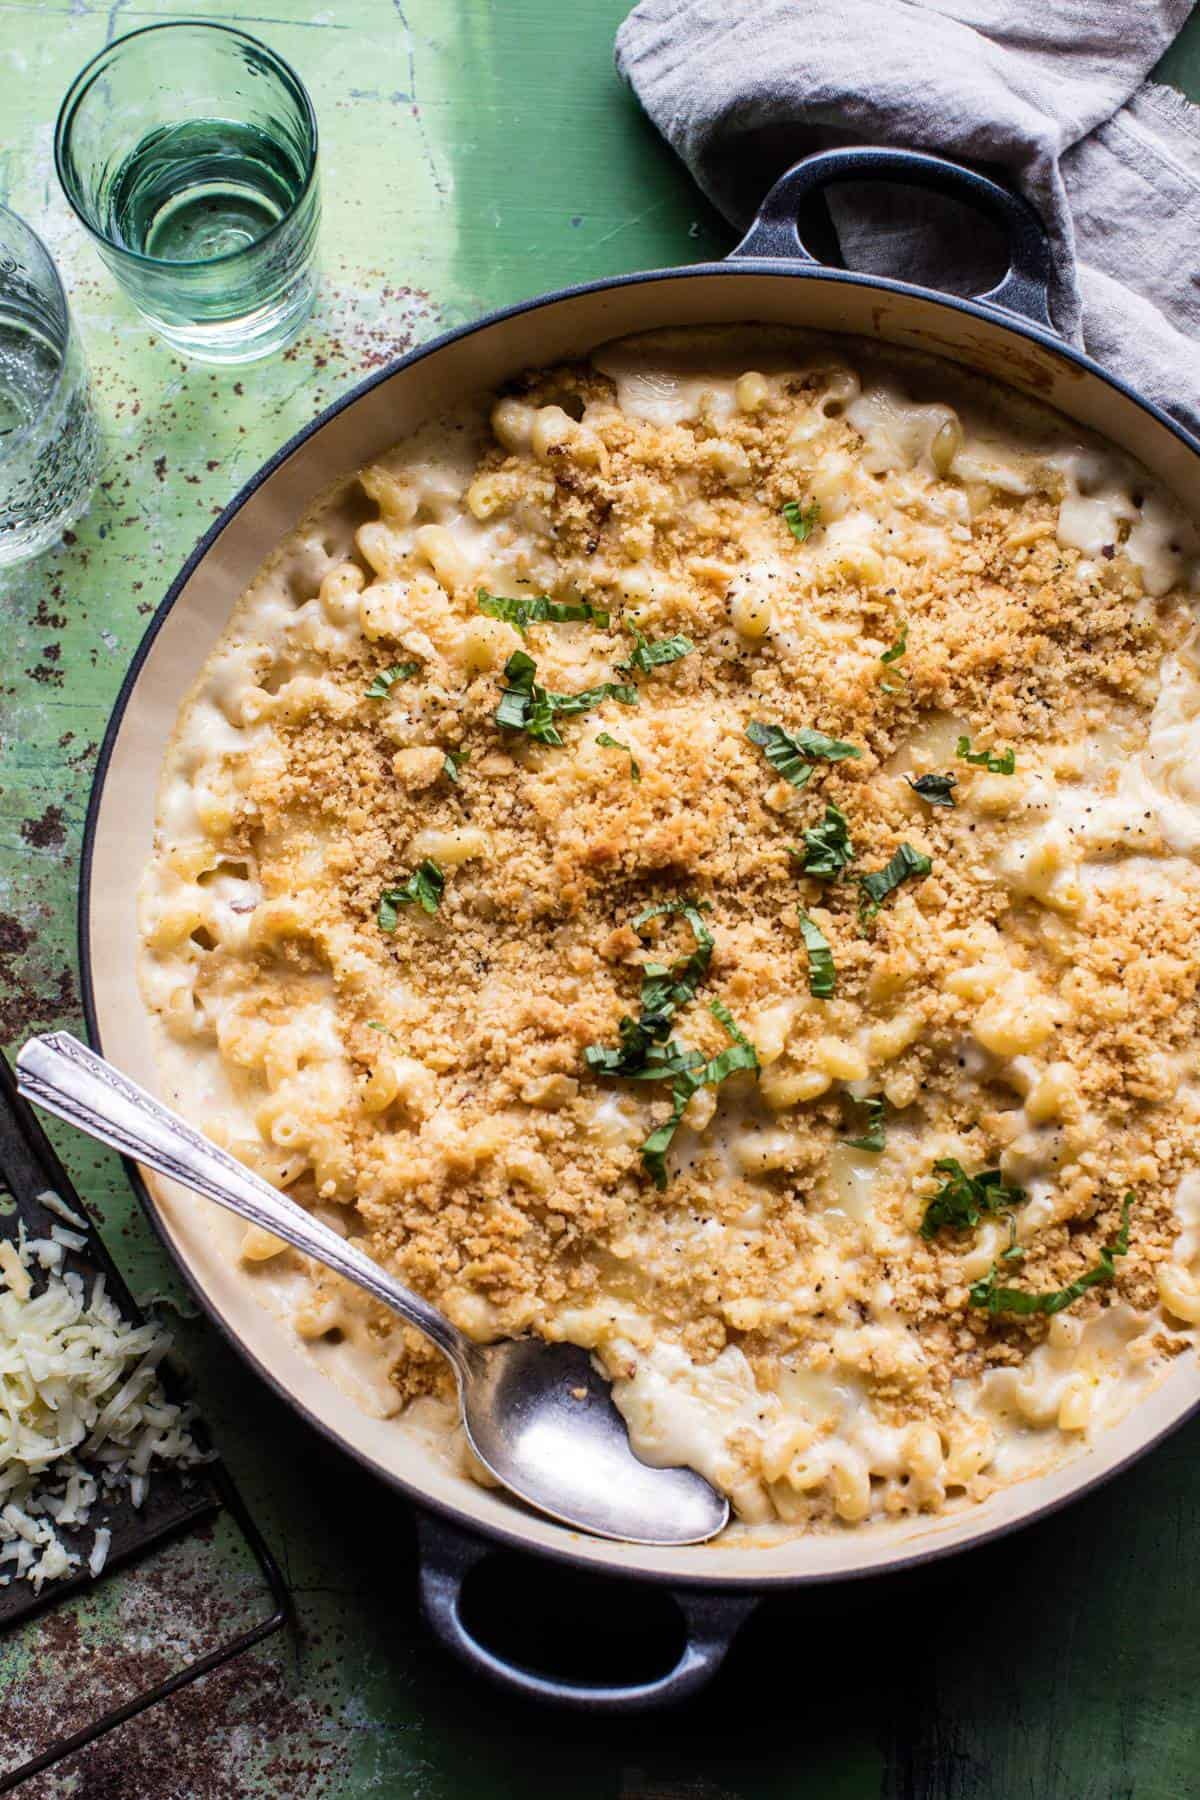
\includegraphics[width=1\textwidth,height=\textheight]{images/the-cheese-maker-s-mac-and-cheese.jpg}

\textbf{Prep Time:} 15 min \textbar{} \textbf{Cook Time:} 45 min
\textbar{} \textbf{Total Time:} 1 hr

\section{Ingredients}\label{ingredients-41}

\begin{itemize}
\tightlist
\item
  7 tablespoons unsalted butter
\item
  ¼ cup all-purpose flour
\item
  3 cups 2\% or whole milk
\item
  1 pound elbow macaroni
\item
  1 garlic clove, minced or grated
\item
  1½ cups crushed Ritz Crackers ((about 1 sleeve))
\item
  4 ounces cream cheese, cut into cubes
\item
  1¼ cups shredded sharp white cheddar cheese
\item
  1¼ cups shredded fontina cheese
\item
  1 cup shredded Havarti cheese
\item
  1 cup shredded smoked Gouda cheese
\item
  ¼ teaspoon cayenne
\item
  Kosher salt and freshly ground pepper
\item
  Fresh basil leaves, for topping
\end{itemize}

\section{Instructions}\label{instructions-41}

\begin{enumerate}
\def\labelenumi{\arabic{enumi}.}
\tightlist
\item
  Preheat the oven to 350°F. Spray a 9 x 13-inch baking dish with
  cooking spray.
\item
  In a large saucepan, melt 4 tablespoons of the butter over medium
  heat. Whisk in the flour. Reduce the heat to medium-low and cook for 1
  minute, stirring once to avoid burning—it will bubble. Gradually whisk
  in the milk and 2 cups of water, then stir in the macaroni. Increase
  the heat to medium-high and bring the mixture to a boil. Stir
  frequently until the macaroni is just al dente, 8 to 10 minutes.
\item
  Meanwhile, in a medium skillet, melt the remaining 3 tablespoons of
  butter over medium-low heat. Add the garlic and cook for 30 seconds,
  or until fragrant. Add the crushed crackers and toss to coat. Toast
  the crumbs until browned, stirring frequently to avoid burning, for 3
  to 5 minutes. Remove the pan from the heat and set aside.
\item
  When the macaroni is al dente, remove the pan from the heat and stir
  in the cream cheese, cheddar, fontina, Havarti, Gouda, and cayenne and
  season with salt and pepper. Stir until the cheeses have fully melted.
  Transfer the mixture to the prepared baking dish.
\item
  Evenly sprinkle the toasted cracker crumbs over the mac and cheese and
  place the baking dish on a baking sheet. Bake for 15 to 20 minutes, or
  until the crumbs are golden brown and the sauce is bubbling. Remove
  from the oven and let sit for 5 minutes (yeah, right). Garnish with
  fresh basil. Dig in!
\end{enumerate}

\bookmarksetup{startatroot}

\chapter{Spinach and Prosciutto Burrata
Calzone}\label{spinach-and-prosciutto-burrata-calzone}

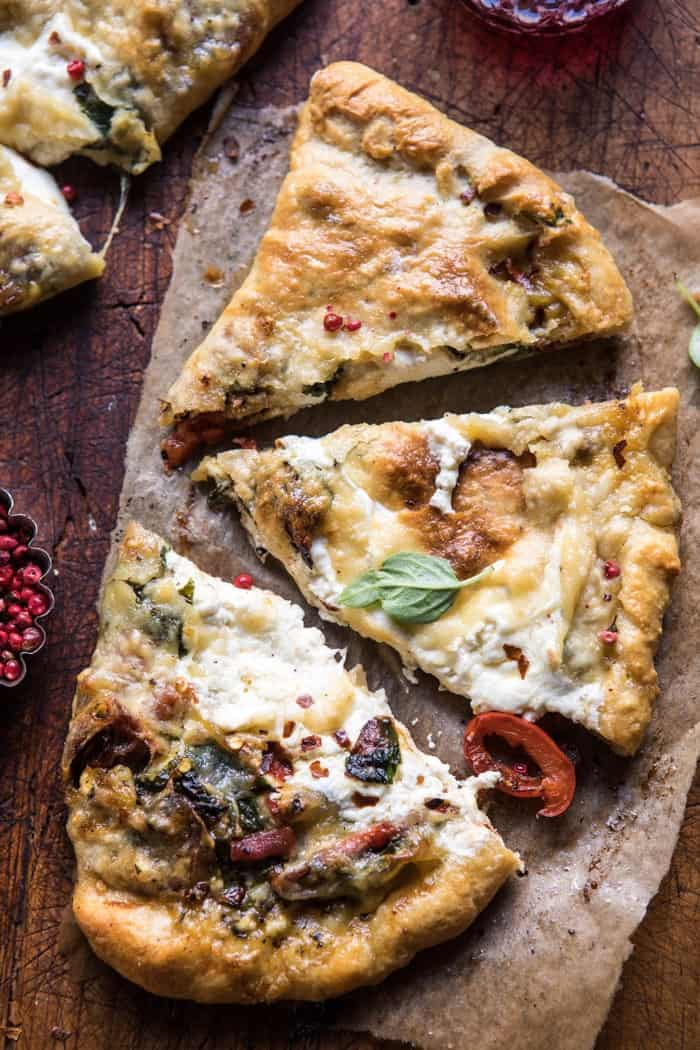
\includegraphics[width=1\textwidth,height=\textheight]{images/spinach-and-prosciutto-burrata-calzone.jpg}

\textbf{Prep Time:} 15 min \textbar{} \textbf{Cook Time:} 20 min
\textbar{} \textbf{Total Time:} 35 min

\section{Ingredients}\label{ingredients-42}

\begin{itemize}
\tightlist
\item
  1 cup shredded fontina cheese
\item
  1/2 cup crumbled goat cheese
\item
  2 cups fresh baby spinach, roughly chopped
\item
  ½ cup jarred roasted red peppers, sliced
\item
  2 ounces prosciutto, chopped
\item
  2 tablespoons extra virgin olive oil, plus more for brushing
\item
  2 cloves garlic, minced or grated
\item
  1 tablespoon chopped fresh rosemary
\item
  zest from 1/2 a lemon
\item
  Kosher salt and pepper
\item
  1 pinch crushed red pepper flakes
\item
  1 pound pizza dough, homemade or store-bought
\item
  2 small/medium balls burrata cheese
\item
  arugula for serving
\end{itemize}

\section{Instructions}\label{instructions-42}

\begin{enumerate}
\def\labelenumi{\arabic{enumi}.}
\tightlist
\item
  Preheat the oven to 450 degrees F.
\item
  In a bowl, combine the fontina, goat cheese, spinach, prosciutto,
  olive oil, garlic, rosemary, lemon zest, and a pinch each of salt and
  pepper, and crushed red pepper flakes.
\item
  Divide the pizza dough into 2 balls. On a lightly floured surface,
  roll each ball of dough out into a large circle about ¼ inch thick.
  Transfer the rounds to a parchment lined baking sheet. Spread half of
  each round of dough evenly with the cheese mix, leaving a ½ inch
  border around the edge of the dough. Add a ball of burrata to the
  filling.
\item
  Using a pastry brush, brush the edges of the dough with water. Fold
  the unfilled side of the dough over the filling and use the tines of a
  fork to seal the dough together. Cut 1-2 slits in the top of each
  calzone and then lightly brush the tops with olive oil. Transfer to
  the oven and bake for 20-25 minutes or until the top is golden brown.
  Top with arugula. Eat!
\end{enumerate}

\bookmarksetup{startatroot}

\chapter{Sweet `n' Savory Roasted Nuts and
Pretzels}\label{sweet-n-savory-roasted-nuts-and-pretzels}

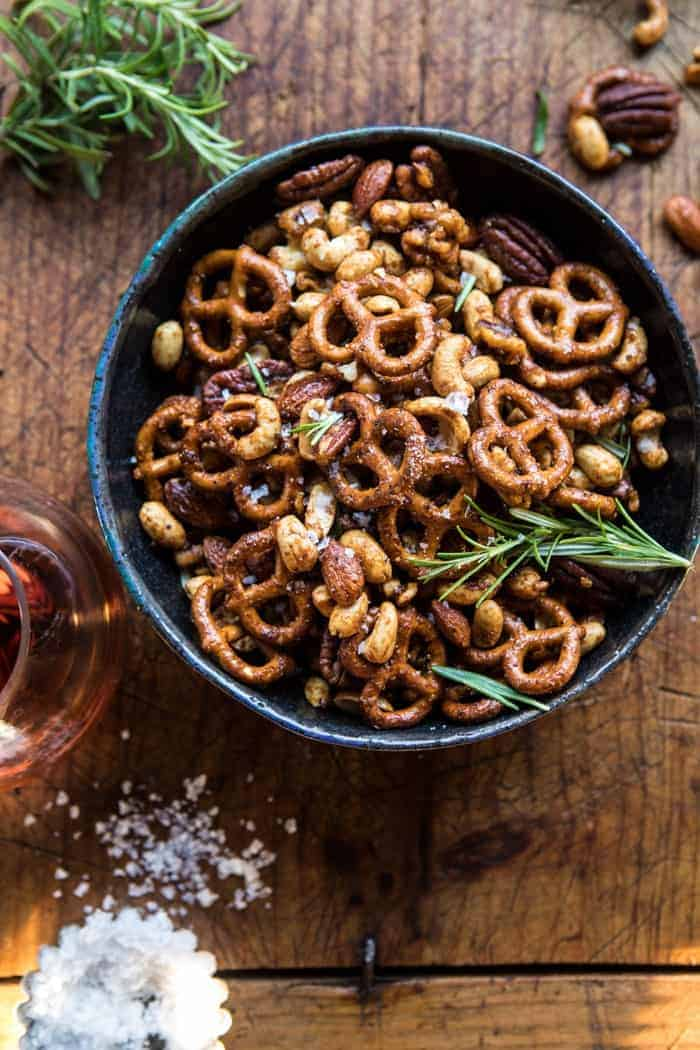
\includegraphics[width=1\textwidth,height=\textheight]{images/sweet-n-savory-roasted-nuts-and-pretzels.jpg}

\textbf{Prep Time:} 10 min \textbar{} \textbf{Cook Time:} 35 min
\textbar{} \textbf{Total Time:} 45 min

\section{Ingredients}\label{ingredients-43}

\begin{itemize}
\tightlist
\item
  4 cups mixed raw nuts
\item
  2 cups pretzel twist
\item
  2 tablespoons salted butter, melted
\item
  2 tablespoons low sodium soy sauce or tamari
\item
  1/4 cup real maple syrup
\item
  1 tablespoon chopped fresh rosemary, plus more for serving
\item
  1 1/2 -2 teaspoons cayenne pepper
\item
  1 1/2 teaspoons chili powder
\item
  1/2 teaspoon smoked paprika
\item
  1/2 teaspoon each onion and garlic powder
\item
  1 teaspoon kosher salt
\end{itemize}

\section{Instructions}\label{instructions-43}

\begin{enumerate}
\def\labelenumi{\arabic{enumi}.}
\tightlist
\item
  Preheat the oven to 350 degrees F.
\item
  On a parchment lined baking sheet, combine the nuts and spread in a
  single layer. Transfer to the oven and roast for 15-20 minutes or
  until lightly golden and toast. Remove from the oven and add the
  pretzels, butter, soy sauce, maple, rosemary, cayenne, chili powder,
  paprika, onion powder, garlic powder, and salt. Toss well to evenly
  combine. Return to the oven and roast for another 10-15 minutes or
  until the nuts are glazed.
\item
  Serve warm with additional rosemary or cool completely and store in an
  air tight container for up to 2 weeks.
\end{enumerate}

\bookmarksetup{startatroot}

\chapter{Brie Stuffed Crispy Baby
Potatoes}\label{brie-stuffed-crispy-baby-potatoes}

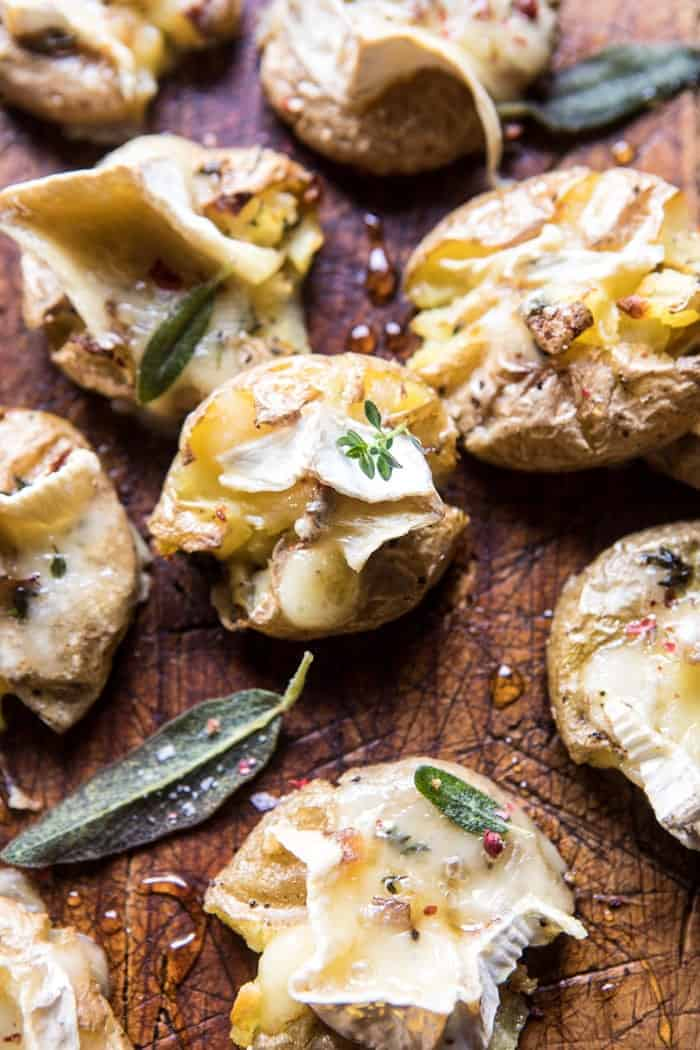
\includegraphics[width=1\textwidth,height=\textheight]{images/brie-stuffed-crispy-baby-potatoes.jpg}

\textbf{Prep Time:} 10 min \textbar{} \textbf{Cook Time:} 45 min
\textbar{} \textbf{Total Time:} 55 min

\section{Ingredients}\label{ingredients-44}

\begin{itemize}
\tightlist
\item
  1 1/2 pounds mixed baby potatoes
\item
  1 tablespoon extra virgin olive oil
\item
  kosher salt and pepper
\item
  3 tablespoons butter, melted
\item
  2 cloves garlic, grated
\item
  2 tablespoons chopped fresh thyme
\item
  8 ounces brie, cut into small wedges
\item
  1-2 teaspoons white truffle oil
\item
  8 pan-fried sage leaves
\item
  crushed pink peppercorn
\end{itemize}

\section{Instructions}\label{instructions-44}

\begin{enumerate}
\def\labelenumi{\arabic{enumi}.}
\tightlist
\item
  Preheat the oven to 400 degrees F.
\item
  On a large baking sheet, toss together the potatoes, olive oil and a
  pinch each of salt and pepper. Transfer to the oven and roast 20
  minutes or until the potatoes are fork tender. Using a potato masher
  or a fork, gently press down on the potatoes, smashing them to about
  1/4 inch thickness.
\item
  Mix together the butter, garlic, and thyme. Drizzle the butter over
  the potatoes and return the potatoes to the oven and roast another
  20-25 minutes or until golden and crisp. During the last 5 minutes of
  cooking, add a thin slice of brie to each potato and roast until
  melted.
\item
  Arrange the warm potatoes on a serving plate and drizzle with truffle
  oil. Top with sage and peppercorns. Enjoy!
\end{enumerate}

\bookmarksetup{startatroot}

\chapter{Cinnamon Streusel Swirled Maple Sweet Potato
Casserole}\label{cinnamon-streusel-swirled-maple-sweet-potato-casserole}

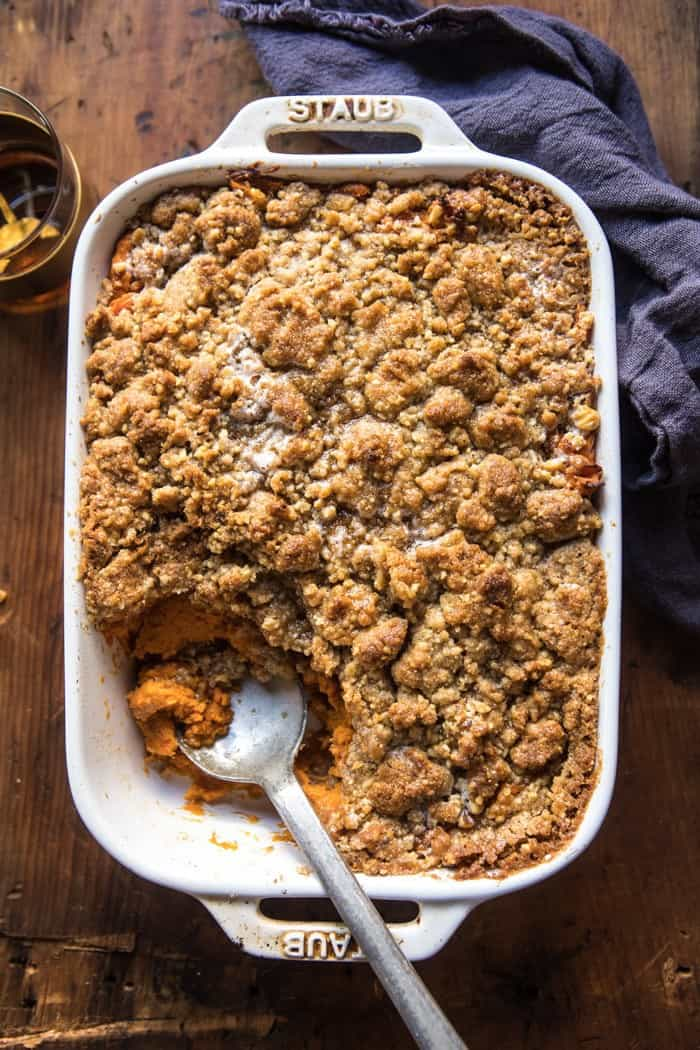
\includegraphics[width=1\textwidth,height=\textheight]{images/cinnamon-streusel-swirled-maple-sweet-potato-casserole.jpg}

\textbf{Prep Time:} 15 min \textbar{} \textbf{Cook Time:} 1 hr
\textbar{} \textbf{Total Time:} 1 hr 15 min

\section{Ingredients}\label{ingredients-45}

\begin{itemize}
\tightlist
\item
  4 medium sweet potatoes
\item
  1/4 cup real maple syrup
\item
  2 teaspoons vanilla extract
\item
  1 teaspoon ground cinnamon
\item
  1/4 cup heavy cream
\item
  4 tablespoons salted butter, melted
\item
  2 eggs, lightly beaten
\item
  1/2 cup all-purpose flour
\item
  1/2 cup brown sugar, packed
\item
  1/2 cup real maple syrup
\item
  1 cup raw walnuts, finely chopped
\item
  1 teaspoon cinnamon
\item
  8 tablespoons cold butter, cubed
\end{itemize}

\section{Instructions}\label{instructions-45}

\begin{enumerate}
\def\labelenumi{\arabic{enumi}.}
\tightlist
\item
  Preheat your oven to 400 degrees F. Grease a 9x13 inch baking dish or
  a dish slighly smaller (no less than 2 quarts).
\item
  Poke a few holes in the sweet potatoes and bake for 1 hour or until
  soft and tender. When the sweet potatoes are cooked, slice them in
  half and allow to cool. Reduce the oven temperature to 350 degrees F.
\item
  Peel the skins away from the sweet potatoes and mash well in a large
  mixing bowl. Mix in the maple syrup, vanilla, cinnamon, heavy cream,
  butter, and eggs, mixing until combined.
\item
  To make the streusel. In a medium bowl, combine the flour, brown sugar
  and cinnamon. Add 6 tablespoons butter and use your fingers to mix the
  butter into the flour until a crumble forms. Stir in 1/4 cup maple
  syrup and the walnuts.
\item
  Pour half the sweet potatoes into the prepared dish. Sprinkle with 1/3
  of the streusel. Spread the remaining sweet potatoes over top and
  sprinkle the remaining streusel evenly over the top of the sweet
  potatoes. Transfer to the oven and bake for 30-40 minutes or until the
  top is dark golden.
\item
  Meanwhile, in a small sauce pan, brown the remaining 2 tablespoons
  butter over medium heat. Stir in the remaining maple syrup.
\item
  Just before serving, drizzle the browned maple butter over the
  casserole. Serve warm.
\end{enumerate}

\bookmarksetup{startatroot}

\chapter{Cranberry Thyme Spritz}\label{cranberry-thyme-spritz}

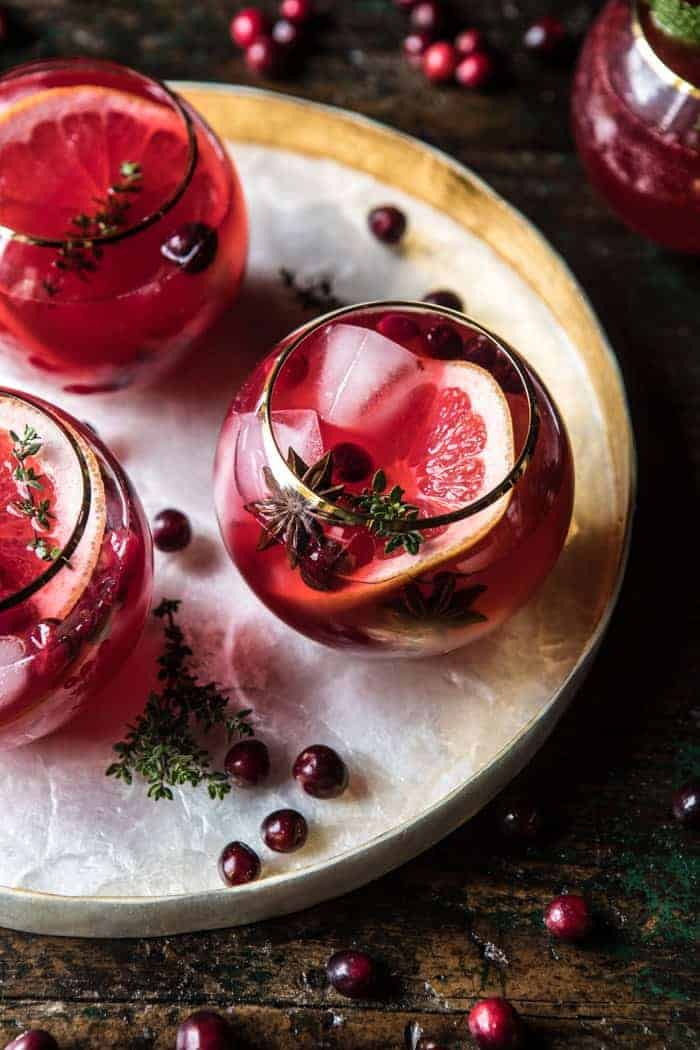
\includegraphics[width=1\textwidth,height=\textheight]{images/cranberry-thyme-spritz.jpg}

\textbf{Prep Time:} 10 min \textbar{} \textbf{Cook Time:} 10 min
\textbar{} \textbf{Total Time:} 20 min

\section{Ingredients}\label{ingredients-46}

\begin{itemize}
\tightlist
\item
  1/2 cup honey
\item
  2 cups fresh cranberries
\item
  2 sprigs fresh thyme
\item
  1 inch fresh ginger, sliced
\item
  8 ounces vodka
\item
  4 ounces elderflower liquor
\item
  1/3 cup fresh squeezed grapefruit juice, plus slices for serving
\item
  1/4 cup fresh lime juice
\item
  4-6 ginger beers
\item
  star anise, for serving ((optional))
\end{itemize}

\section{Instructions}\label{instructions-46}

\begin{enumerate}
\def\labelenumi{\arabic{enumi}.}
\tightlist
\item
  In a medium pot, bring 1/2 cup water, the honey, cranberries, thyme,
  and ginger to a boil over high heat. Boil 5 minutes or until the
  cranberries begin to burst, then remove from the heat. Let cool.
  Remove the thyme and ginger. If desired, strain out the cranberries.
\item
  In a large pitcher, combine the cranberry syrup mix, vodka,
  elderflower liquor, grapefruit juice, and lime juice. Chill until
  ready to serve.
\item
  Add the ginger beer just before serving. Garnish each drink with a
  grapefruit slice and star anise, if desired.
\end{enumerate}

\bookmarksetup{startatroot}

\chapter{Pomegranate Avocado Salad with Candied
Walnuts}\label{pomegranate-avocado-salad-with-candied-walnuts}

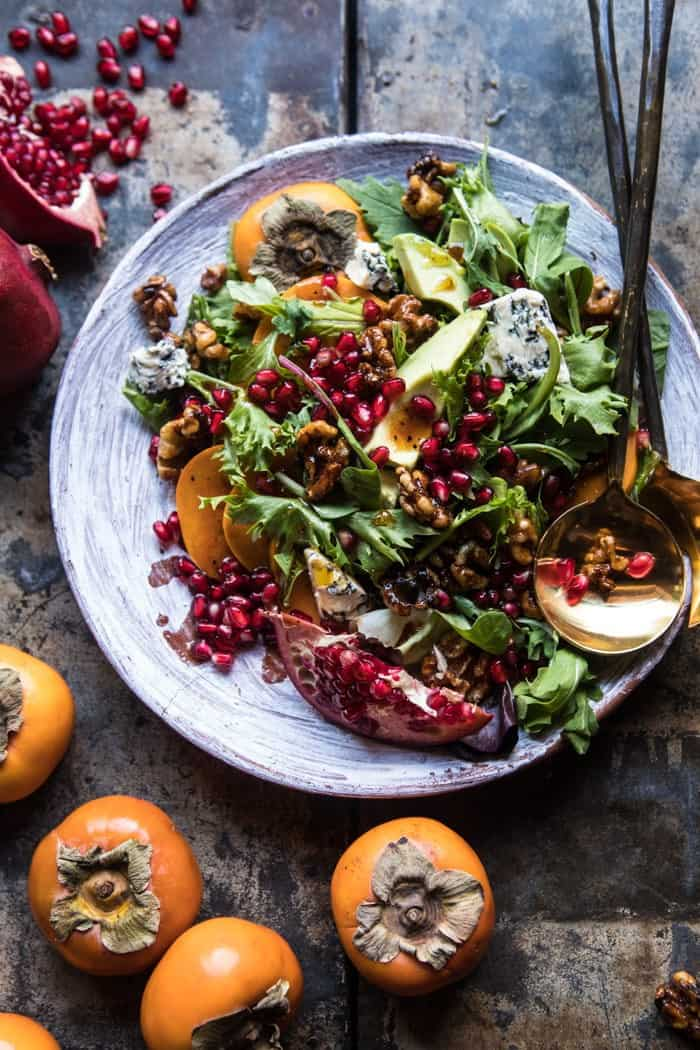
\includegraphics[width=1\textwidth,height=\textheight]{images/pomegranate-avocado-salad-with-candied-walnuts.jpg}

\textbf{Prep Time:} 15 min \textbar{} \textbf{Cook Time:} 15 min
\textbar{} \textbf{Total Time:} 30 min

\section{Ingredients}\label{ingredients-47}

\begin{itemize}
\tightlist
\item
  1 1/2 cups raw walnuts
\item
  1/3 cup real maple syrup
\item
  1/2 teaspoon cayenne pepper
\item
  6 cups mustard greens or mixed greens
\item
  2 cups baby arugula
\item
  2 persimmons, thinly sliced
\item
  1 avocado, sliced
\item
  arils from 1-2 pomegranates
\item
  6 ounces blue cheese, crumbed ((or goat cheese or feta))
\item
  1/3 cup extra virgin olive oil
\item
  2 tablespoons balsamic vinegar or red wine vinegar
\item
  2 tablespoons pomegranate juice
\item
  2 teaspoons orange zest
\item
  kosher salt and pepper to taste
\end{itemize}

\section{Instructions}\label{instructions-47}

\begin{enumerate}
\def\labelenumi{\arabic{enumi}.}
\tightlist
\item
  Preheat the oven 375 degrees F. Line a baking sheet with parchment
  paper. Add the walnuts to the baking sheet and toss with the maple
  syrup, cayenne and a pinch of salt. Bake for 15-20 minutes, stirring
  2-3 time throughout cooking until the walnuts are toasted and golden.
  Remove from the oven and spread the walnuts in one layer. Allow to
  cool.
\item
  Add the greens to a large bowl. Add the persimmons, avocado,
  pomegranate arils, walnuts, and blue cheese. Give the salad a gentle
  toss.
\item
  To make the vinaigrette, combine the olive oil, balsamic vinegar,
  pomegranate juice, orange zest, and a pinch each of salt an pepper in
  a bowl or glass jar. Drizzle the dressing over the salad or serve
  along side the salad. Enjoy!
\end{enumerate}

\bookmarksetup{startatroot}

\chapter{Butternut Squash and Sun-Dried Tomato White
Lasagna}\label{butternut-squash-and-sun-dried-tomato-white-lasagna}

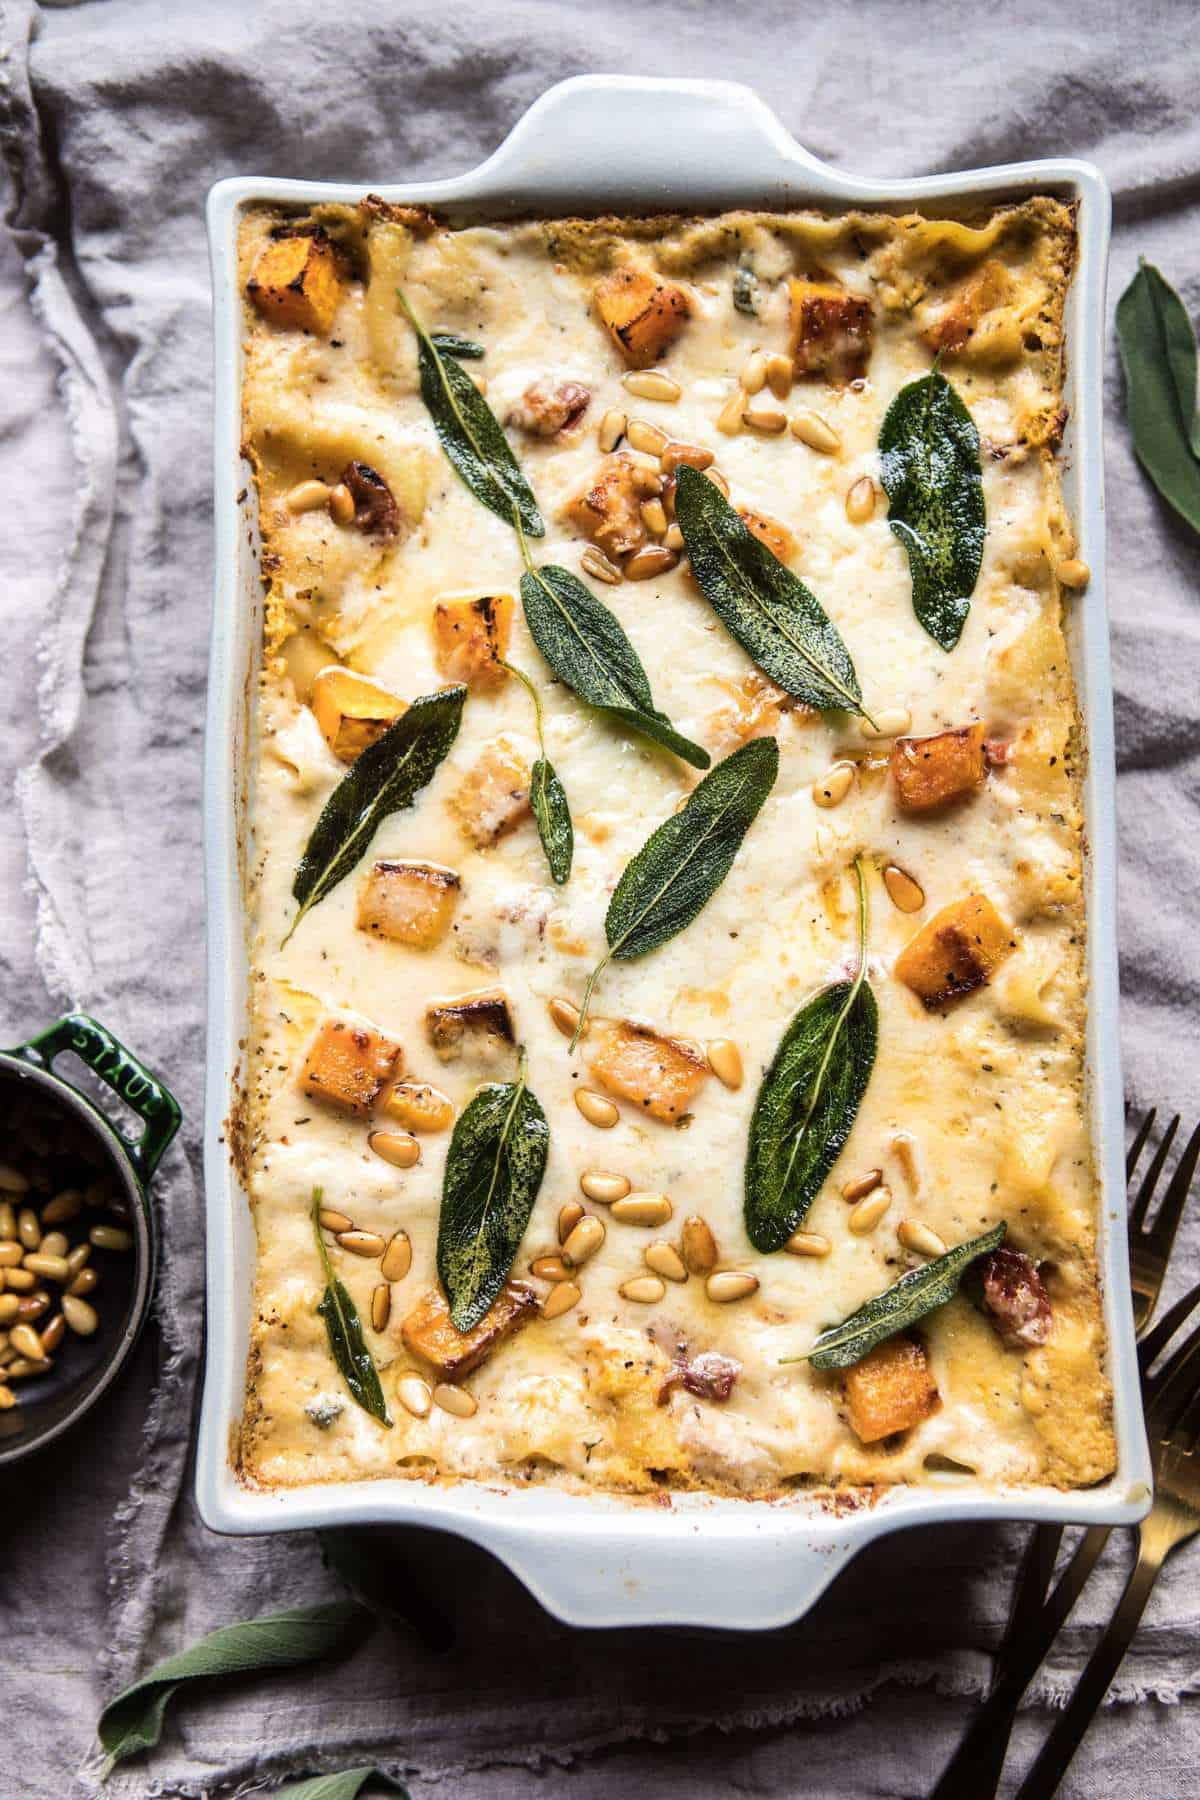
\includegraphics[width=1\textwidth,height=\textheight]{images/butternut-squash-and-sun-dried-tomato-white-lasagna.jpg}

\textbf{Prep Time:} 30 min \textbar{} \textbf{Cook Time:} 1 hr 30 min
\textbar{} \textbf{Total Time:} 2 hr

\section{Ingredients}\label{ingredients-48}

\begin{itemize}
\tightlist
\item
  4 cups butternut squash, cubed ((about 1 medium squash))
\item
  2 tablespoons extra virgin olive oil
\item
  1 tablespoon honey
\item
  kosher salt and pepper
\item
  6 tablespoons butter
\item
  2 cloves garlic, minced or grated
\item
  1 tablespoon fresh sage, chopped
\item
  1 tsp dried basil
\item
  1/4 cup flour
\item
  3 1/2 cups whole milk
\item
  1/4 teaspoon fresh grated nutmeg
\item
  1 cup shredded fontina cheese
\item
  1 cup parmesan cheese, grated
\item
  2 cups whole milk ricotta
\item
  2 cups shredded provolone
\item
  1 jar (8 ounce) oil packed sun-dried tomatoes, oil drained and chopped
\item
  1 box no-boil lasagna noodles
\item
  2 tablespoons toasted pine nuts
\end{itemize}

\section{Instructions}\label{instructions-48}

\begin{enumerate}
\def\labelenumi{\arabic{enumi}.}
\tightlist
\item
  Preheat oven to 375 degrees F. Grease a 9x13 inch pan.
\item
  On a baking sheet, toss together the butternut squash, olive oil,
  honey, and a pinch each of salt and pepper. Transfer to the oven and
  roast for 25-30 minutes or until the squash is tender.
\item
  Melt the butter in a medium sauce pan. Add the garlic, sage, and basil
  and cook 30 seconds or until fragrant. Whisk in the flour and cook for
  about 1 minute. Slowly add the milk. Stir in the nutmeg and season
  with salt and pepper. Bring to a boil and stir for 1 minute. Remove
  from heat and stir in the fontina cheese and 1/2 cup of parmesan
  cheese. Stir until the cheese is fully melted and the sauce is smooth.
  Set the cheese sauce aside.
\item
  In a medium bowl, mash the roasted butternut squash until mostly
  smooth. Stir in the ricotta, provolone, and sun-dried tomatoes.
\item
  Spread 1/4 of the cheese sauce in the bottom of the prepared baking
  dish. Top with 3-4 lasagna sheets. Spread with 1/2 the butternut
  squash mixture and then another 1/4 of the cheese sauce. Place another
  3-4 lasagna noodles on top, and then top with the remaining butternut
  squash mixture and another 1/4 of the cheese sauce. Add the remaining
  lasagna noodles and pour the remaining 1/4 of the cheese sauce over
  top. Top with the remaining 1/2 cup of parmesan cheese. Bake uncovered
  for 45 minutes or until the top has bubbled up and browned a bit. Let
  stand 10 minutes before serving. Top with pine nuts and fried sage.
\end{enumerate}

\bookmarksetup{startatroot}

\chapter{Easy Flaky Pull-Apart Dinner
Rolls}\label{easy-flaky-pull-apart-dinner-rolls}

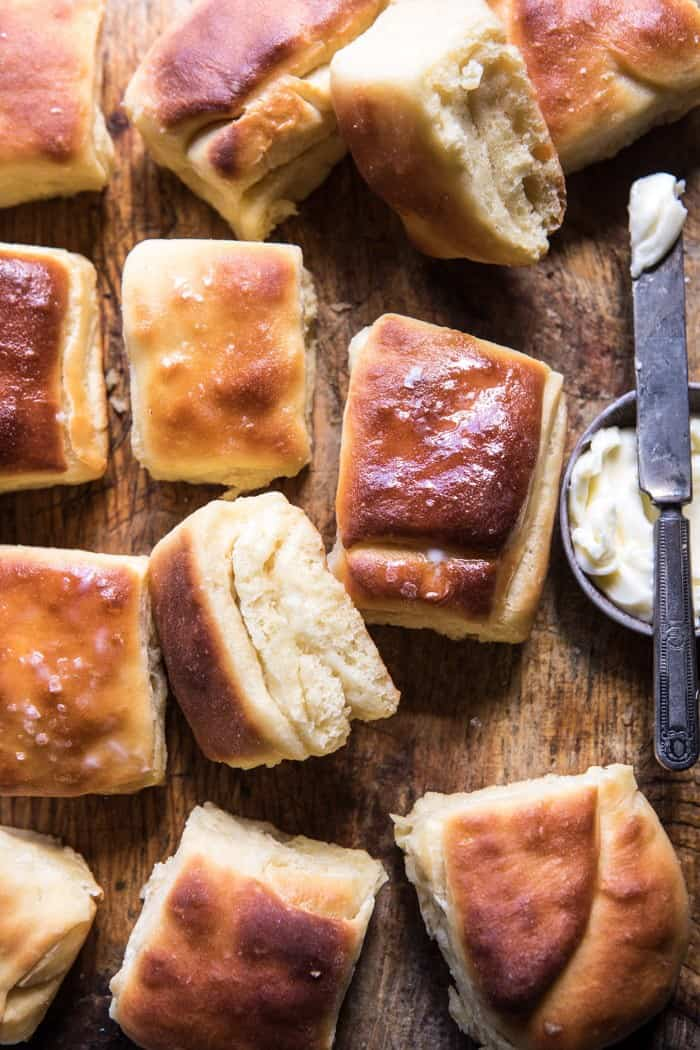
\includegraphics[width=1\textwidth,height=\textheight]{images/easy-flaky-pull-apart-dinner-rolls.jpg}

\textbf{Prep Time:} 15 min \textbar{} \textbf{Cook Time:} 25 min
\textbar{} \textbf{Total Time:} 40 min

\section{Ingredients}\label{ingredients-49}

\begin{itemize}
\tightlist
\item
  1 cup warm whole milk
\item
  2 1/2 teaspoons instant yeast
\item
  2 tablespoons honey
\item
  2 large eggs
\item
  3-4 cups all-purpose flour
\item
  1/2 teaspoon kosher salt
\item
  6 tablespoons salted butter, at room temperature, plus melted butter
  for brushing
\item
  flaky sea salt, for topping ((optional))
\end{itemize}

\section{Instructions}\label{instructions-49}

\begin{enumerate}
\def\labelenumi{\arabic{enumi}.}
\tightlist
\item
  In the bowl of a stand mixer, combine the milk, yeast, honey, eggs,
  flour, and salt. Using the dough hook, mix until the flour is
  completely incorporated, about 4-5 minutes. Add 2 tablespoons butter
  and mix until combined, about 2-3 minutes more.
\item
  Cover the bowl with plastic wrap and let sit at room temperature for 1
  hour or until doubled in size.
\item
  Grease a 9x13 inch baking dish with butter.
\item
  Punch the dough down and roll out on a lightly floured surface into a
  large rectangle that’s about 1/4 inch thick. Spread the remaining 4
  tablespoons of softened butter all over dough, being careful not to
  break through the dough with butter.
\item
  Fold one half of the rectangle towards the center and fold the other
  half over the top of the first layer so you have three dough layers.
  Cut the dough into 12 equal squares. Arrange in the prepared baking
  dish. Cover the pan, and let the rolls rise for about 45 minutes to 1
  hour, until they're puffy. Alternately, you can place the pan in the
  fridge to rise overnight.
\item
  reheat the oven to 350. Bake the rolls for 20 to 25 minutes, until
  they're golden brown on top.
\item
  Remove them from the oven, and brush with the melted butter, sprinkle
  with salt, of desired. Pull them apart to serve warm.
\end{enumerate}

\bookmarksetup{startatroot}

\chapter{Honey Butter Roasted Acorn with Burrata and
Pomegranate}\label{honey-butter-roasted-acorn-with-burrata-and-pomegranate}

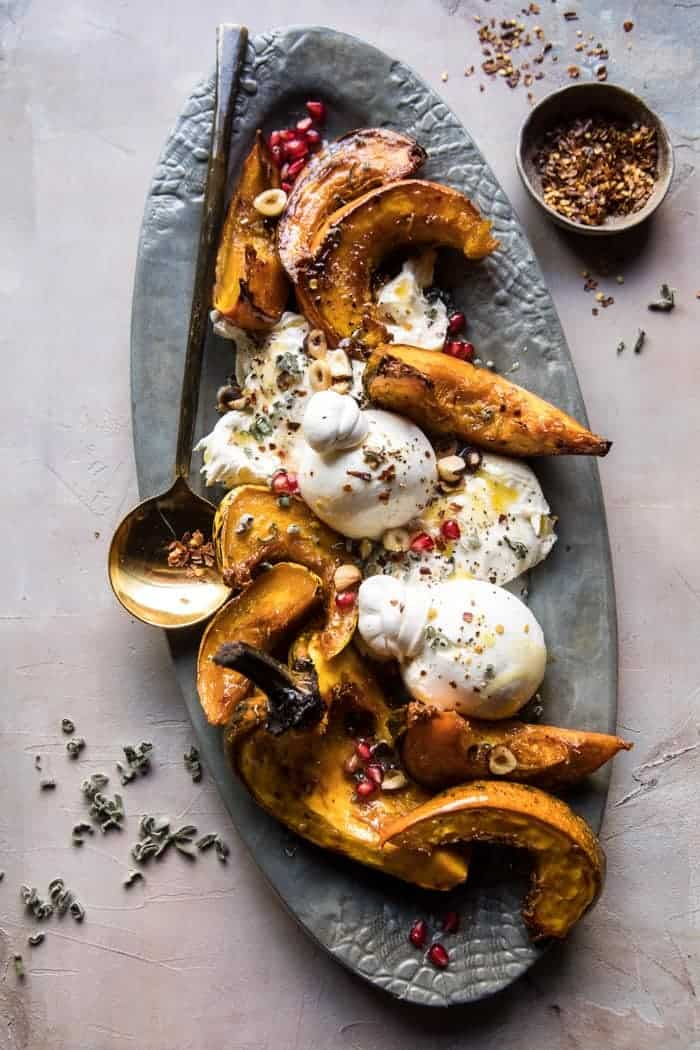
\includegraphics[width=1\textwidth,height=\textheight]{images/honey-butter-roasted-acorn-with-burrata-and-pomegranate.jpg}

\textbf{Prep Time:} 10 min \textbar{} \textbf{Cook Time:} 30 min
\textbar{} \textbf{Total Time:} 40 min

\section{Ingredients}\label{ingredients-50}

\begin{itemize}
\tightlist
\item
  2 acorn squash, seeded and cut into wedges
\item
  4 tablespoons butter
\item
  2 tablespoons honey, plus more for drizzling
\item
  1 tablespoon brown sugar
\item
  1/2-1 teaspoon crushed red pepper flakes, to taste
\item
  kosher salt and pepper
\item
  2-3 balls burrata cheese
\item
  extra virgin olive oil, for drizzling
\item
  4 fresh sage leaves, chopped
\item
  1/2 cup roasted, salted hazelnuts, roughly chopped
\item
  1/2 cup pomegranate arils
\end{itemize}

\section{Instructions}\label{instructions-50}

\begin{enumerate}
\def\labelenumi{\arabic{enumi}.}
\tightlist
\item
  Preheat the oven to 425 degrees F.
\item
  On a baking sheet, toss together the squash, butter, honey, brown
  sugar, crushed red pepper flakes, and a pinch each of kosher salt and
  pepper, tossing to coat. Transfer to the oven and roast for 30-40
  minutes, until the squash is golden and tender, turning halfway
  through cooking.
\item
  Arrange the squash on a serving platter and break the balls of burrata
  over the top. Drizzle with olive oil and season the burrata with salt
  and pepper. Sprinkle the sage, hazelnuts, and pomegranate over top. If
  desired, drizzle with a little honey. Serve!
\end{enumerate}

\bookmarksetup{startatroot}

\chapter{Pappardelle with Roasted Butternut Squash and Tomato
Ragu}\label{pappardelle-with-roasted-butternut-squash-and-tomato-ragu}

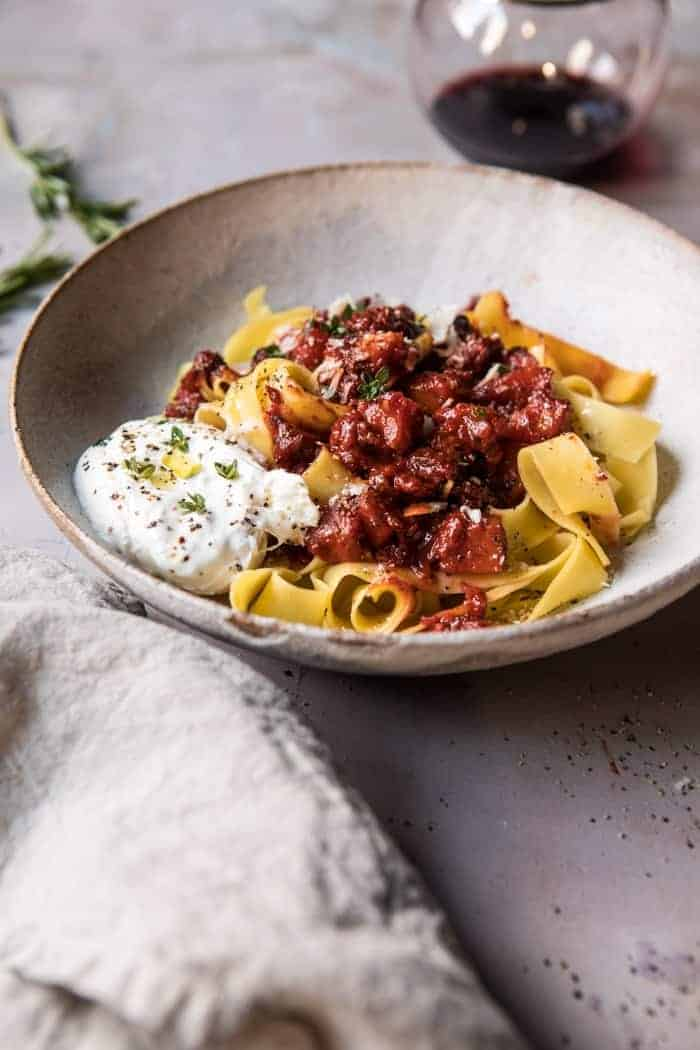
\includegraphics[width=1\textwidth,height=\textheight]{images/pappardelle-with-roasted-butternut-squash-and-tomato-ragu.jpg}

\textbf{Prep Time:} 15 min \textbar{} \textbf{Cook Time:} 45 min
\textbar{} \textbf{Total Time:} 1 hr

\section{Ingredients}\label{ingredients-51}

\begin{itemize}
\tightlist
\item
  2 tablespoons extra virgin olive oil
\item
  1 pound ground spicy Italian sausage
\item
  1/2 sweet onion, chopped
\item
  3 garlic cloves, smashed
\item
  kosher salt and pepper
\item
  1 1/2 cups cubed butternut squash
\item
  1 can (28 ounce) San Marzano tomatoes
\item
  1/2 cup red wine
\item
  1 bay leaf
\item
  4 fresh sage leaves
\item
  2 fresh thyme sprigs
\item
  4 tablespoons butter
\item
  1 pound Pappardelle or your favorite cut of pasta
\item
  burrata cheese and parmesan cheese, for serving
\end{itemize}

\section{Instructions}\label{instructions-51}

\begin{enumerate}
\def\labelenumi{\arabic{enumi}.}
\tightlist
\item
  Preheat the oven to 425 degrees F.
\item
  Heat the olive oil in a large skillet set over medium heat. When the
  oil shimmers, add the sausage, onion, and garlic and cook until the
  sausage has browned all over, about 8-10 minutes. Season with salt and
  pepper. Stir in the butternut squash and continue cooking until the
  squash is golden on the edges, about 5 minutes. Remove from the heat
  and stir in all of the tomatoes, wine, bay leaf, sage, and thyme.
  Arrange the butter slices over top.
\item
  Transfer to the oven and roast for 30-35 minutes or until the squash
  is soft and the sauce thickened. Remove the bay leaf and thyme sprigs.
\item
  Meanwhile, bring a large pot of salted water to a boil. Cook the pasta
  according to package directions until al dente. Drain. Stir the pasta
  into the Ragu sauce.
\item
  Divide the pasta among plates and top with burrata and parmesan. EAT.
\end{enumerate}

\bookmarksetup{startatroot}

\chapter{Pan Roasted Brussels Sprouts with Bacon, Dates, and
Halloumi}\label{pan-roasted-brussels-sprouts-with-bacon-dates-and-halloumi}

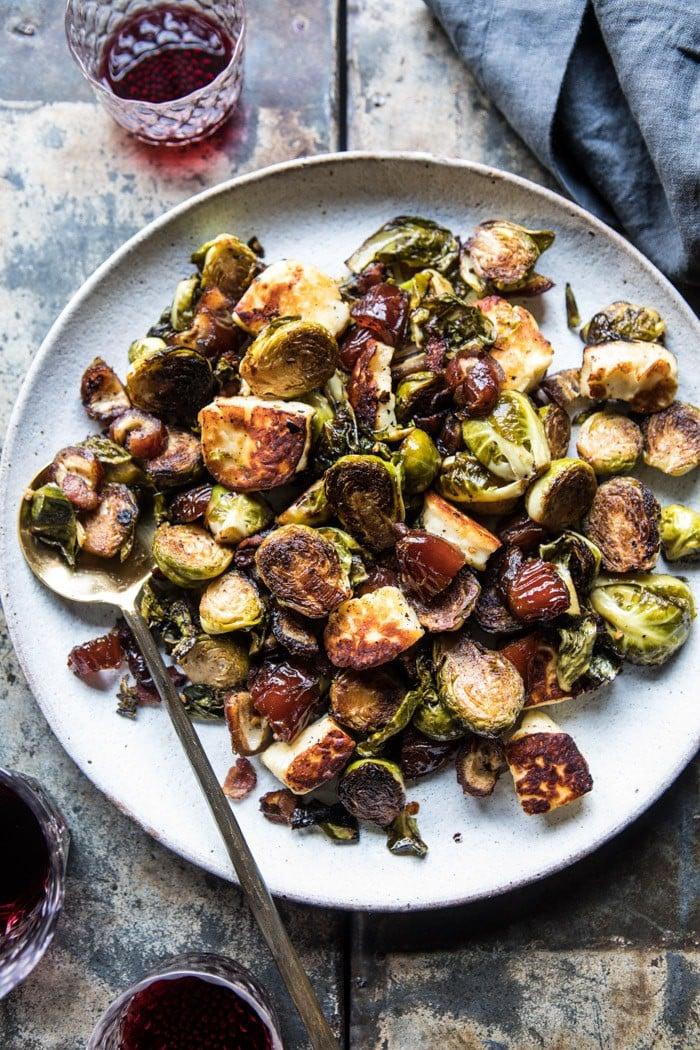
\includegraphics[width=1\textwidth,height=\textheight]{images/pan-roasted-brussels-sprouts-with-bacon-dates-and-halloumi.jpg}

\textbf{Prep Time:} 15 min \textbar{} \textbf{Cook Time:} 25 min
\textbar{} \textbf{Total Time:} 40 min

\section{Ingredients}\label{ingredients-52}

\begin{itemize}
\tightlist
\item
  2 slices thick cut bacon, chopped
\item
  1 pound brussels sprouts, halved
\item
  3 tablespoons extra virgin olive oil
\item
  kosher salt and pepper
\item
  1/2 teaspoon crushed red pepper flakes
\item
  1/3 cup medjool dates, pits removed and chopped
\item
  1/4 cup red wine vinegar
\item
  8 ounces Halloumi cheese, cubed
\end{itemize}

\section{Instructions}\label{instructions-52}

\begin{enumerate}
\def\labelenumi{\arabic{enumi}.}
\tightlist
\item
  Heat a large 12-inch skillet over medium high heat. Add the bacon and
  cook until crisp and the fat has rendered, about 5 minutes. Remove the
  bacon from the skillet and drain on a pepper towel lined plate.
\item
  Add 2 tablespoons olive oil to the skillet with the bacon grease. When
  the oil shimmers, add the brussels sprouts, cut side down and cook
  until charred around the edges, about 5-8 minutes. It is OK if the
  brussels sprouts become blackened in some parts. Stir and season with
  salt and pepper. Continue cooking another 8-10 minutes or until the
  brussels sprouts are soft. Reduce the heat to medium and stir in the
  crushed red pepper flakes, dates, and red wine vinegar. Cook until the
  vinegar coats the brussels sprouts, about 1-2 minutes. Remove from the
  heat.
\item
  Heat a small skillet over medium heat and add 1 tablespoon olive oil.
  When the oil shimmers, add the Halloumi cheese and sear for 2-3
  minutes per side until golden. Stir the cheese into the brussels
  sprouts. Serve warm. Enjoy!
\end{enumerate}

\bookmarksetup{startatroot}

\chapter{Roasted Cranberry Brown Sugar Pork
Chops.}\label{roasted-cranberry-brown-sugar-pork-chops.}

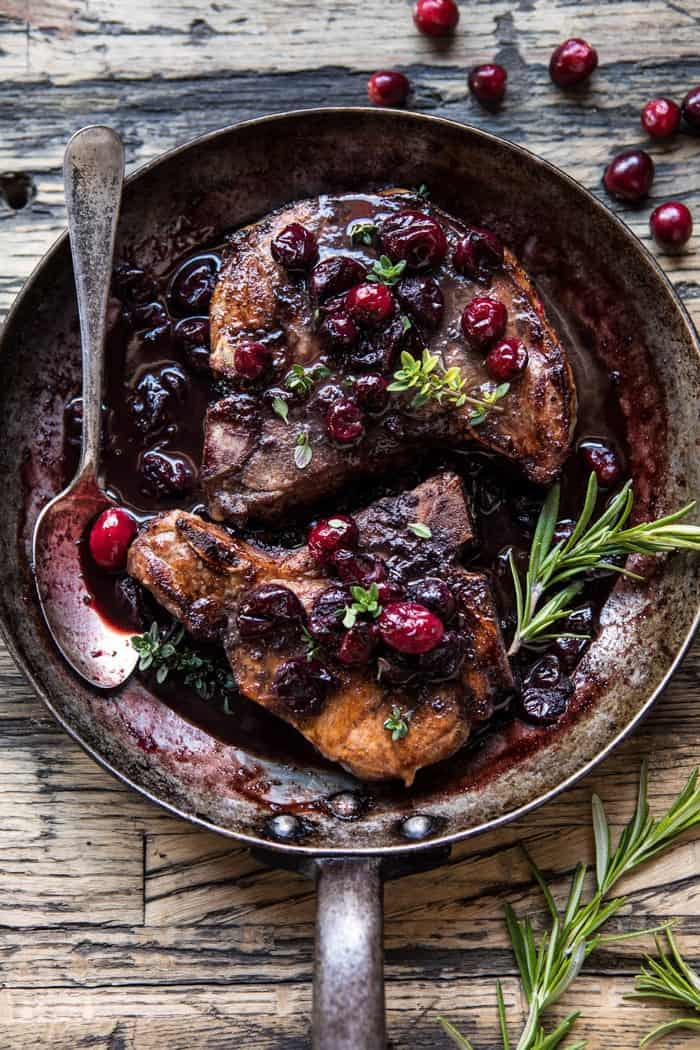
\includegraphics[width=1\textwidth,height=\textheight]{images/roasted-cranberry-brown-sugar-pork-chops-.jpg}

\textbf{Prep Time:} 10 min \textbar{} \textbf{Cook Time:} 20 min
\textbar{} \textbf{Total Time:} 30 min

\section{Ingredients}\label{ingredients-53}

\begin{itemize}
\tightlist
\item
  4 tablespoons brown sugar
\item
  1 teaspoon cayenne pepper
\item
  1/2 teaspoon cinnamon
\item
  kosher salt and pepper
\item
  4 bone-in pork chops
\item
  2 tablespoons extra-virgin olive oil
\item
  3/4 cup red wine
\item
  1/2 cup pomegranate or cranberry juice
\item
  2 tablespoons butter
\item
  1 cup fresh cranberries
\item
  2 sprigs fresh thyme
\item
  1 sprig fresh rosemary
\end{itemize}

\section{Instructions}\label{instructions-53}

\begin{enumerate}
\def\labelenumi{\arabic{enumi}.}
\tightlist
\item
  Preheat the oven to 450 degrees.
\item
  In a small bowl, stir together 3 tablespoons brown sugar, the cayenne,
  cinnamon, and a large pinch of both salt and pepper. Place the pork
  chops on a cutting board and rub them all over with the brown sugar
  mixture.
\item
  Heat the olive oil in a large skillet over high heat. When the oil
  shimmers, add the pork chops and sear for 2 to 4 minutes per side or
  until golden brown. Remove the pork chops from the skillet and set
  aside.
\item
  To the skillet, slowly pour in the wine and pomegranate juice. Add the
  remaining 1 tablespoon brown sugar, the butter, cranberries, thyme,
  and rosemary. Season with salt. Bring the sauce to a boil over high
  heat. Reduce the heat to medium and slide the pork chops into the
  sauce, cook for a minute longer and remove from heat.
\item
  Transfer the skillet to the oven and roast for 10-15 minutes or until
  the chops are lightly charred and the sauce thickened. Serve the chops
  with the pan sauce spooned over top.
\end{enumerate}

\bookmarksetup{startatroot}

\chapter{Caramelized Garlic Butter Toast with Pan Fried
Mushrooms}\label{caramelized-garlic-butter-toast-with-pan-fried-mushrooms}

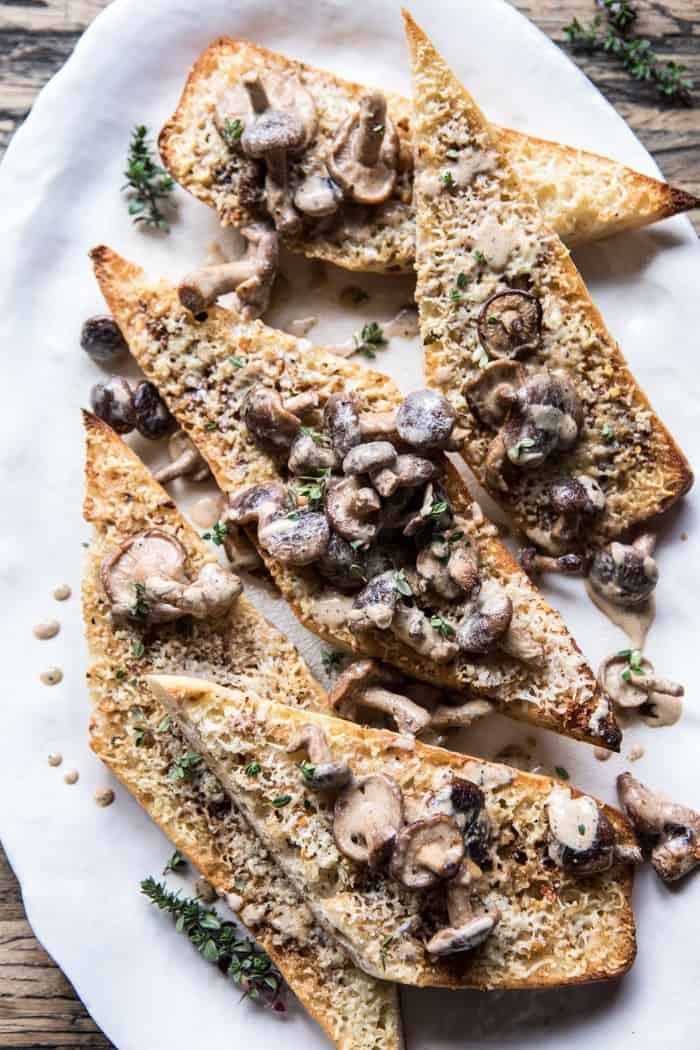
\includegraphics[width=1\textwidth,height=\textheight]{images/caramelized-garlic-butter-toast-with-pan-fried-mushrooms.jpg}

\textbf{Prep Time:} 15 min \textbar{} \textbf{Cook Time:} 30 min
\textbar{} \textbf{Total Time:} 45 min

\section{Ingredients}\label{ingredients-54}

\begin{itemize}
\tightlist
\item
  1 stick (1/2 cup) salted butter
\item
  4-6 cloves garlic
\item
  2 teaspoons chopped fresh oregano
\item
  1/2 teaspoon crushed red pepper flakes
\item
  1 sourdough baguette, halved lengthwise and cut in 6 pieces
\item
  1 cup grated parmesan cheese
\item
  1 tablespoon extra virgin olive oil
\item
  1 pound mixed mushrooms
\item
  2 teaspoons chopped fresh thyme, plus more for serving
\item
  kosher salt and pepper
\item
  1/4 cup white wine
\item
  1/4 cup buttermilk
\item
  1/4 cup heavy cream
\end{itemize}

\section{Instructions}\label{instructions-54}

\begin{enumerate}
\def\labelenumi{\arabic{enumi}.}
\tightlist
\item
  Preheat the oven to 425 degrees F.
\item
  In a large skillet, combine the butter, garlic, and oregano. Cook over
  medium low heat, stirring often until the garlic is golden and
  caramelized, about 15 minutes. The butter will brown slightly. Remove
  from the heat and finely mash the garlic with a fork. Stir in the
  crushed red pepper flakes.
\item
  Arrange the bread on a baking sheet. Drizzle/rub the garlic butter
  onto each cut side of bread. Top with cheese and transfer to the oven
  for 8-10 minutes or until the cheese has melted.
\item
  Meanwhile, return the skillet to medium heat and add the olive oil.
  When the oil shimmers, add the mushrooms. Cooking, undistributed until
  the mushrooms are golden on the bottom, about 3-5 minutes, stir and
  add the thyme and a pinch each of salt and pepper. Reduce the heat to
  low, add the wine, buttermilk, and cream. Cook until warmed though,
  about 5 minutes. Remove from the heat and season as needed with salt
  and pepper.
\item
  Arrange the garlic bread on a serving plate and spoon the mushrooms
  over top. Alternately, you can serve the garlic bread alongside the
  mushrooms for dipping/spoon over the bread. Top with thyme. EAT!
\end{enumerate}

\bookmarksetup{startatroot}

\chapter{Roasted Squash, Caramelized Fig, and Feta
Salad}\label{roasted-squash-caramelized-fig-and-feta-salad}

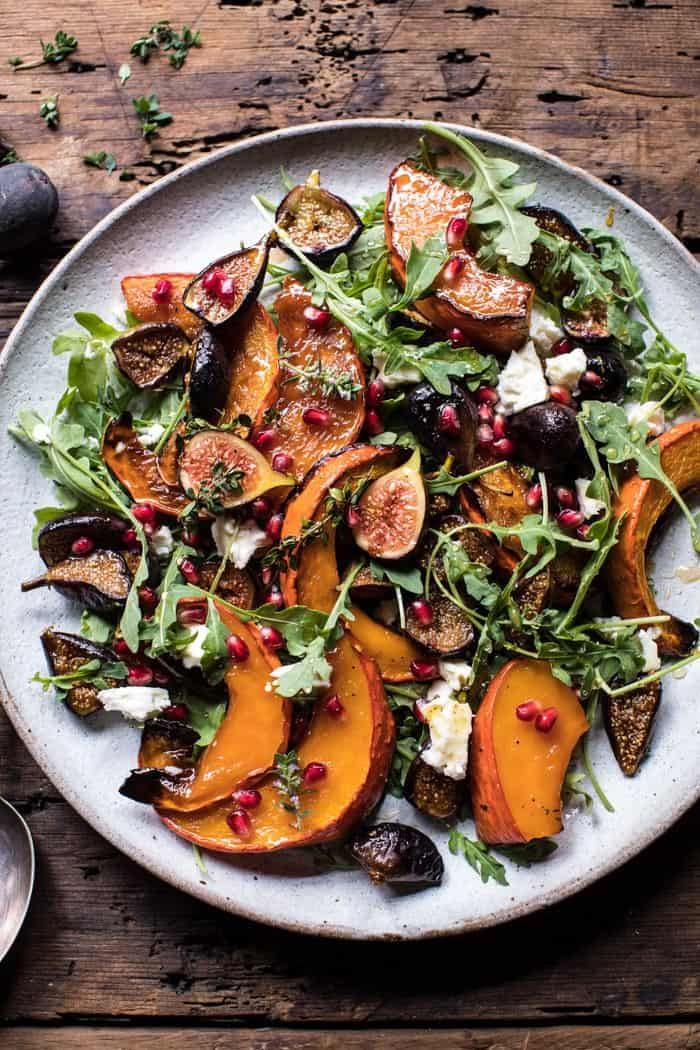
\includegraphics[width=1\textwidth,height=\textheight]{images/roasted-squash-caramelized-fig-and-feta-salad.jpg}

\textbf{Prep Time:} 15 min \textbar{} \textbf{Cook Time:} 30 min
\textbar{} \textbf{Total Time:} 45 min

\section{Ingredients}\label{ingredients-55}

\begin{itemize}
\tightlist
\item
  1 kabocha or acorn squash, sliced
\item
  1/4 cup + 2 tablespoons extra virgin olive oil
\item
  1/4 cup honey
\item
  2 tablespoons fresh thyme leaves
\item
  kosher salt
\item
  16-20 fresh or dried figs, halved
\item
  2 tablespoons lemon juice
\item
  2 tablespoons apple cider vinegar
\item
  1 tablespoon orange zest
\item
  black pepper
\item
  4 cups baby arugula
\item
  4 ounces feta cheese crumbles
\item
  arils from 1 pomegranate
\end{itemize}

\section{Instructions}\label{instructions-55}

\begin{enumerate}
\def\labelenumi{\arabic{enumi}.}
\tightlist
\item
  Preheat the oven to 425 degrees F.
\item
  On a rimmed baking sheet, toss together the squash, 2 tablespoons
  olive oil, honey, 1 1/2 tablespoons thyme leaves, and a good pinch of
  salt. Transfer to the oven and roast for 20 minutes. Remove from the
  oven, add the figs to the baking sheet and toss to combine. Return to
  the oven and roast another 10-15 minutes or until the figs have
  caramelized. If using dried figs, cook them only 5 minutes. This will
  soften them.
\item
  To make the dressing: In a mason jar, combine the remaining 1/4 cup
  olive oil, lemon juice, apple cider vinegar, remaining 1/2 tablespoon
  thyme, orange zest, and a pinch each of kosher salt and pepper.
\item
  Add the arugula to a large salad bowl and top with the roasted squash
  and figs. Crumble the feta overtop and sprinkle with pomegranate
  arils. Drizzle with the dressing. Enjoy!
\end{enumerate}

\bookmarksetup{startatroot}

\chapter{Brussels Sprout Mushroom Pizza with Crispy Prosciutto and
Sage}\label{brussels-sprout-mushroom-pizza-with-crispy-prosciutto-and-sage}

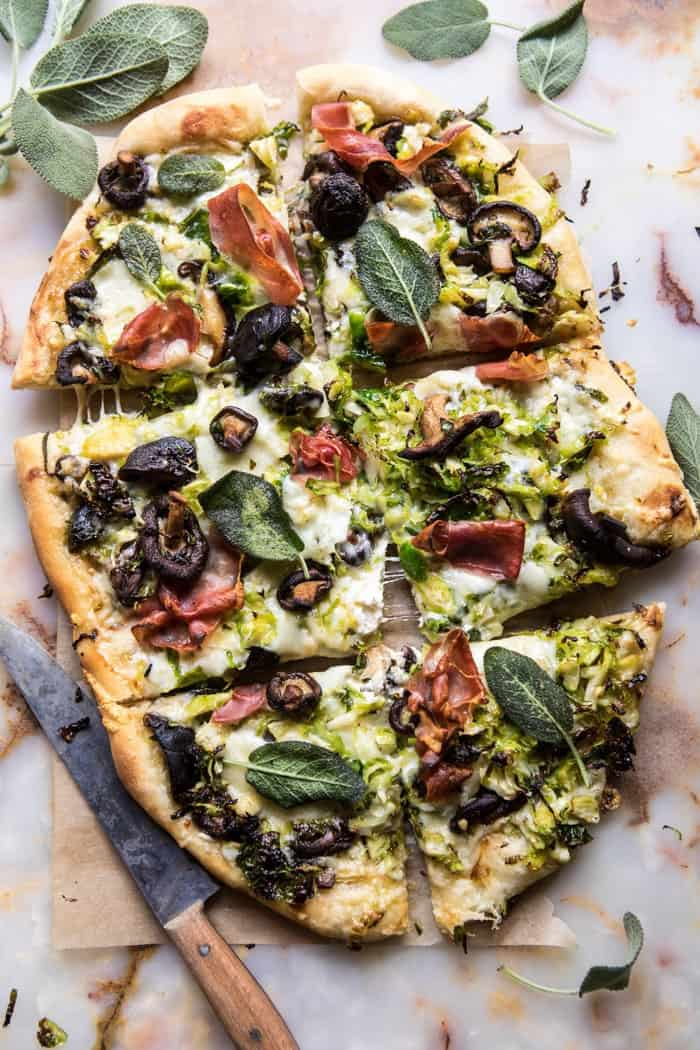
\includegraphics[width=1\textwidth,height=\textheight]{images/brussels-sprout-mushroom-pizza-with-crispy-prosciutto-and-sage.jpg}

\textbf{Prep Time:} 20 min \textbar{} \textbf{Cook Time:} 15 min
\textbar{} \textbf{Total Time:} 35 min

\section{Ingredients}\label{ingredients-56}

\begin{itemize}
\tightlist
\item
  3 tablespoons extra virgin olive oil
\item
  8 fresh sage leaves
\item
  1 pound mixed wild mushrooms or cremini mushrooms, sliced
\item
  kosher salt and pepper
\item
  2 tablespoons butter
\item
  1 clove garlic, minced or grated
\item
  1/2 cup fresh herbs, roughly chopped ((I like basil and thyme))
\item
  1 pound brussels sprouts, shredded
\item
  1/2 pound pizza dough, homemade or store-bought
\item
  2 tablespoons apple butter
\item
  1 pinch crushed red pepper flakes
\item
  8 ounces fresh burrata cheese
\item
  1 1/2 cups shredded provolone cheese
\item
  3 ounces prosciutto, torn
\end{itemize}

\section{Instructions}\label{instructions-56}

\begin{enumerate}
\def\labelenumi{\arabic{enumi}.}
\tightlist
\item
  Preheat the oven to 450 degrees F. Grease a large baking sheet with
  olive oil.
\item
  Heat 2 tablespoon olive oil in a large skillet over high heat. When
  the oil shimmers, add the sage, fry 30 seconds. Remove from the
  skillet and set aside for serving. To the same skillet, add the
  mushrooms and season with salt and pepper. Cook undisturbed for 5
  minutes or until golden, stir and continue cooking until the mushrooms
  have caramelized, 3-5 minutes. Reduce the heat to medium. Add the
  butter, garlic, and herbs. Cook, stirring occasionally until the
  garlic is caramelized and fragrant, about 5 minutes. Remove from the
  heat.
\item
  In a medium bowl, toss together the shredded brussels sprouts, the
  remaining 1 tablespoon olive oil, and a pinch each of salt and pepper.
\item
  On a lightly floured surface, push/roll the dough out until it is
  pretty thin (about a 10-12 inch circle). Transfer the dough to the
  baking sheet. Spread the apple butter over the dough. Break the ball
  of burrata over the dough and then arrange the mushrooms and brussels
  sprouts over top. Sprinkle on the provolone and the top with
  prosciutto.
\item
  Transfer to the oven and bake for 10-15 minutes or until the crust is
  golden and the cheese has melted. Top with fried sage. EAT!
\end{enumerate}

\bookmarksetup{startatroot}

\chapter{Pan Roasted Pomegranate Glazed
Salmon}\label{pan-roasted-pomegranate-glazed-salmon}

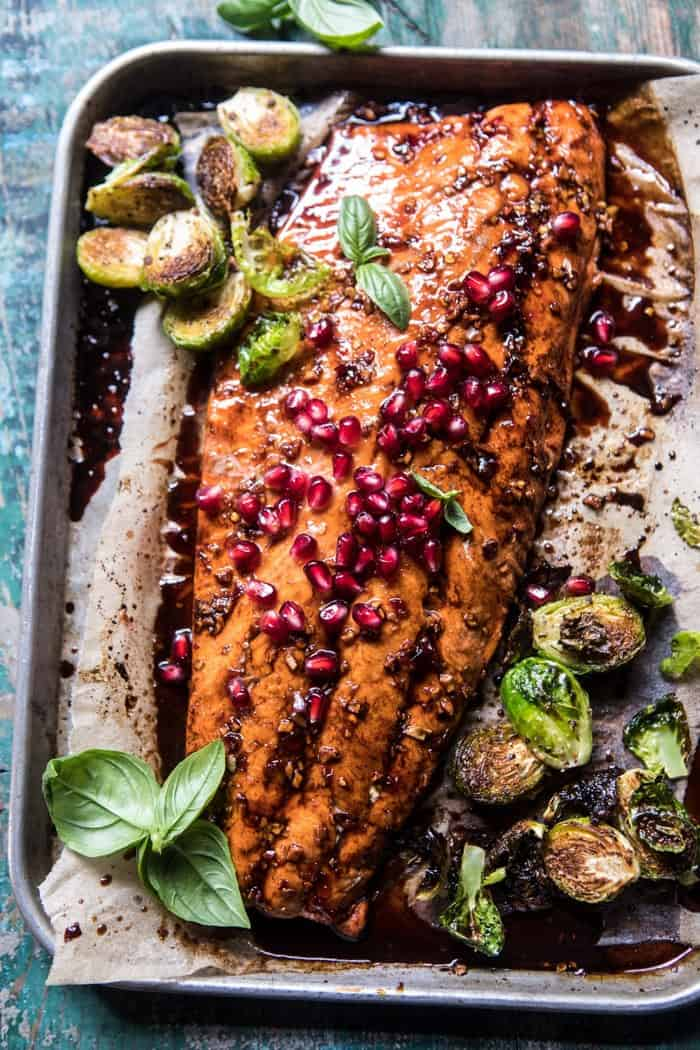
\includegraphics[width=1\textwidth,height=\textheight]{images/pan-roasted-pomegranate-glazed-salmon.jpg}

\textbf{Prep Time:} 10 min \textbar{} \textbf{Cook Time:} 20 min
\textbar{} \textbf{Total Time:} 30 min

\section{Ingredients}\label{ingredients-57}

\begin{itemize}
\tightlist
\item
  1 pound brussels sprouts, halved
\item
  2 tablespoons extra virgin olive oil
\item
  kosher salt and pepper
\item
  2 tablespoons pomegranate molasses
\item
  2 tablespoons sweet chili sauce
\item
  2 tablespoons pomegranate juice
\item
  1 inch fresh ginger, grated
\item
  1 clove garlic, minced or grated
\item
  1 pinch red pepper flakes
\item
  1 pound wild caught salmon
\item
  fresh basil for serving
\end{itemize}

\section{Instructions}\label{instructions-57}

\begin{enumerate}
\def\labelenumi{\arabic{enumi}.}
\tightlist
\item
  Preheat oven to 425 degrees F.
\item
  On a large rimmed baking sheet, combine the brussels sprouts, olive
  oil, and a pinch each of salt and pepper. Toss well to evenly coat.
  Place in the oven and roast for 15 minutes.
\item
  Meanwhile, combine the pomegranate molasses, pomegranate juice, sweet
  chili sauce, ginger, garlic, and a pinch each of red pepper flakes and
  salt in a small bowl.
\item
  Remove the brussels sprouts from the oven. Add the salmon to the
  center of the pan. Spoon the pomegranate glaze over the salmon.
  Transfer to the oven and roast for 10-20 minutes or until the salmon
  has reached your desired doneness.
\item
  Top the salmon with pomegranate arils and fresh basil. Enjoy!
\end{enumerate}

\bookmarksetup{startatroot}

\chapter{Healthy 5 Ingredient
Buckeyes}\label{healthy-5-ingredient-buckeyes}

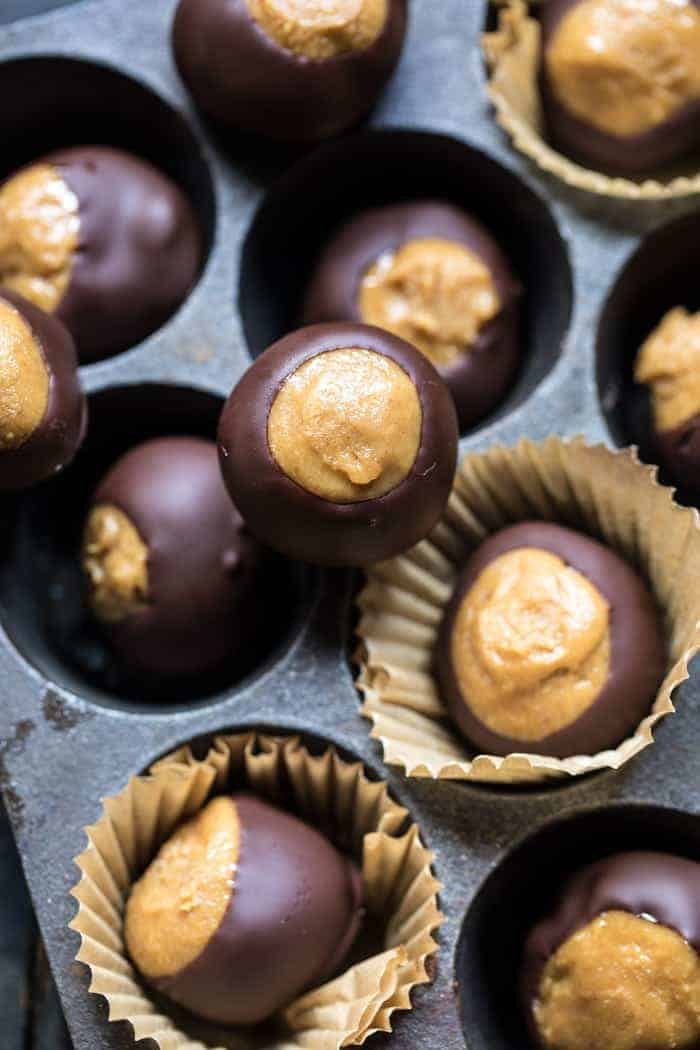
\includegraphics[width=1\textwidth,height=\textheight]{images/healthy-5-ingredient-buckeyes.jpg}

\textbf{Prep Time:} 20 min \textbar{} \textbf{Cook Time:} 1 hr
\textbar{} \textbf{Total Time:} 1 hr 20 min

\section{Ingredients}\label{ingredients-58}

\begin{itemize}
\tightlist
\item
  1 1/2 cups creamy peanut butter
\item
  1/4 cup honey
\item
  2-4 tablespoons softened butter, to your taste
\item
  1 teaspoon vanilla extract
\item
  2 cups chopped dark chocolate, melted
\end{itemize}

\section{Instructions}\label{instructions-58}

\begin{enumerate}
\def\labelenumi{\arabic{enumi}.}
\tightlist
\item
  In the bowl of a stand mixer, combine the peanut butter, honey,
  butter, and vanilla and beat until smooth and creamy. The mix will be
  runny.
\item
  Scoop tablespoon size amounts of dough out and roll into a rough ball.
  Place on the parchment lined baking sheet. Repeat with the remaining
  dough, cover and place in the freezer for 20 minutes.
\item
  After 20 minutes, remove the balls from the freezer and roll them once
  more between your hands to smooth the balls out. Return to the freezer
  for at least 45 minutes, being sure they are very cold before coating
  in chocolate.
\item
  Stick a toothpick into the top of each ball. Working with one ball at
  a time, dip the frozen balls into the chocolate leaving a small
  opening at the top so the peanut butter can peek out. Place the balls
  back on the baking sheet. Repeat with the remaining balls. Store in
  the fridge until ready to eat. These are best straight out of the
  fridge. Enjoy!
\end{enumerate}

\bookmarksetup{startatroot}

\chapter{Late Summer Vegetable Bolognese with Creamy
Polenta}\label{late-summer-vegetable-bolognese-with-creamy-polenta}

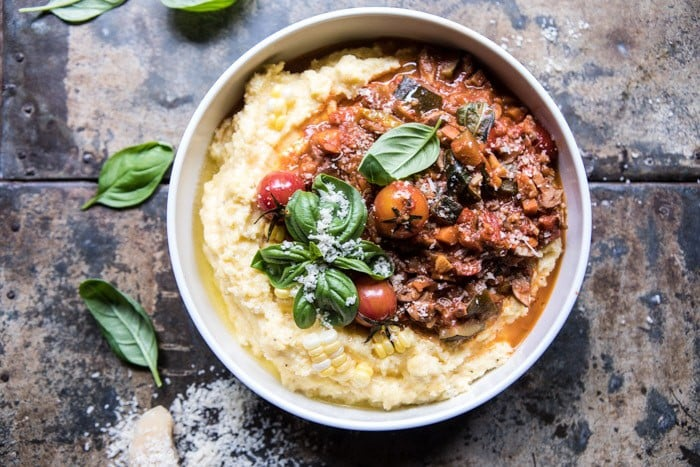
\includegraphics[width=1\textwidth,height=\textheight]{images/late-summer-vegetable-bolognese-with-creamy-polenta.jpg}

\textbf{Prep Time:} 15 min \textbar{} \textbf{Cook Time:} 30 min
\textbar{} \textbf{Total Time:} 45 min

\section{Ingredients}\label{ingredients-59}

\begin{itemize}
\tightlist
\item
  4 tablespoons extra virgin olive oil
\item
  1 small sweet onion, diced
\item
  2 carrots, chopped
\item
  1 zucchini, chopped
\item
  1 bell pepper, chopped
\item
  2 cups cremini mushrooms, chopped
\item
  4 cloves garlic, minced or grated
\item
  2 tablespoons chopped fresh thyme
\item
  kosher salt and pepper
\item
  1 (28 ounce) can san marzano tomatoes
\item
  1 cup cherry tomatoes
\item
  1 cup white wine
\item
  1/2 cup raw walnuts, chopped
\item
  1 handful fresh basil
\item
  2 cups whole milk
\item
  1 cup instant polenta
\item
  2 ears corn, kernels removed
\item
  2 tablespoons butter
\item
  kosher salt and pepper
\end{itemize}

\section{Instructions}\label{instructions-59}

\begin{enumerate}
\def\labelenumi{\arabic{enumi}.}
\tightlist
\item
  Heat the olive oil in a large skillet set over medium heat.
\item
  When the oil shimmers, add the onions and carrots and cook until
  softened, about 5 minutes. Stir in the zucchini, bell peppers,
  mushrooms, garlic, and thyme. Season with salt and pepper. Cook for
  8-10 minutes or until the veggies are tender.
\item
  Stir in all of the tomatoes, wine, and 1/2 cup water. Stir in the
  walnuts. Shimmer the sauce for 20 minutes or until it has thickened
  and the tomatoes have burst. Season with salt and pepper and then stir
  in the basil.
\item
  Meanwhile, make the polenta. In a medium saucepan bring 2 cups of
  water and the milk to a boil over medium heat. Slowly whisk in the
  polenta, stirring, until the polenta is soft and thick, about 5
  minutes. Stir in the corn and butter until melted. Season with salt
  and pepper.
\item
  Ladle the bolognese over the polenta. Enjoy!
\end{enumerate}

\bookmarksetup{startatroot}

\chapter{Chicken Broccoli Quinoa
Casserole}\label{chicken-broccoli-quinoa-casserole}

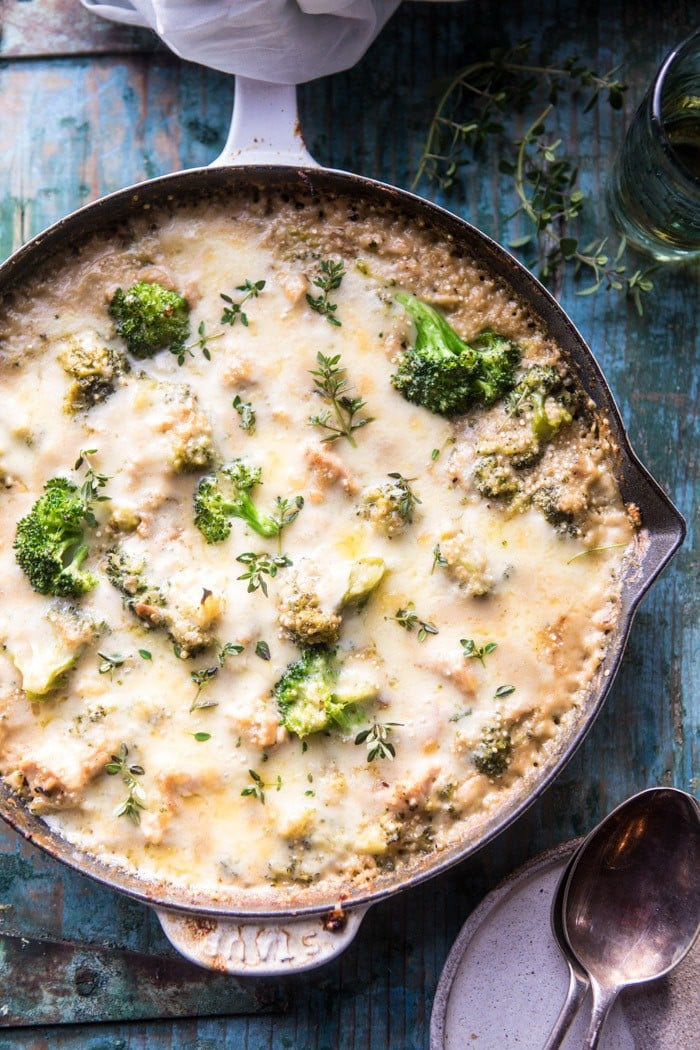
\includegraphics[width=1\textwidth,height=\textheight]{images/chicken-broccoli-quinoa-casserole.jpg}

\textbf{Prep Time:} 15 min \textbar{} \textbf{Cook Time:} 40 min
\textbar{} \textbf{Total Time:} 55 min

\section{Ingredients}\label{ingredients-60}

\begin{itemize}
\tightlist
\item
  2 tablespoons extra virgin olive oil
\item
  1 pound boneless chicken breasts, cut into cubes
\item
  kosher salt and pepper
\item
  1/2 sweet onion, diced
\item
  1 cup cremini mushrooms, roughly chopped
\item
  2 tablespoons all purpose flour
\item
  1 1/2 cups whole milk
\item
  1 cup low sodium chicken broth
\item
  3/4 cup dry quinoa
\item
  2 cups roughly chopped broccoli
\item
  1 tablespoon chopped fresh thyme, plus more for topping
\item
  1/2 teaspoon garlic powder
\item
  1 cup shredded cheddar cheese
\item
  1/4 cup grated parmesan cheese
\end{itemize}

\section{Instructions}\label{instructions-60}

\begin{enumerate}
\def\labelenumi{\arabic{enumi}.}
\tightlist
\item
  Preheat the broiler to high.
\item
  Heat the olive oil in a large skillet set over medium heat. When the
  oil shimmers, add the chicken and season with salt and pepper. Cook
  8-10 minutes, stirring occasionally until the chicken is cooked
  through. Remove the chicken from the skillet.
\item
  To the skillet, add the remaining 1 tablespoon olive oil, onion, and
  mushrooms. Season with salt and pepper. Cook, stirring occasionally
  until the onion is fragrant and the mushrooms have caramelized, about
  5 minutes. Stir in the flour and cook 1 minute.
\item
  Slowly pour in the milk and chicken broth and bring to a simmer. Add
  the quinoa, broccoli, thyme, and garlic powder. Stir back in the
  chicken. Reduce the heat to low, cover and cook 15-20 minutes or until
  the quinoa is tender. Remove from the heat and add the cheese.
  Transfer to the oven and broil for 2-3 minutes or until the cheese has
  melted.
\item
  Top with fresh thyme and EAT!
\end{enumerate}

\bookmarksetup{startatroot}

\chapter{Lightened Up Salsa Verde Chicken Stuffed Poblano
Peppers}\label{lightened-up-salsa-verde-chicken-stuffed-poblano-peppers}

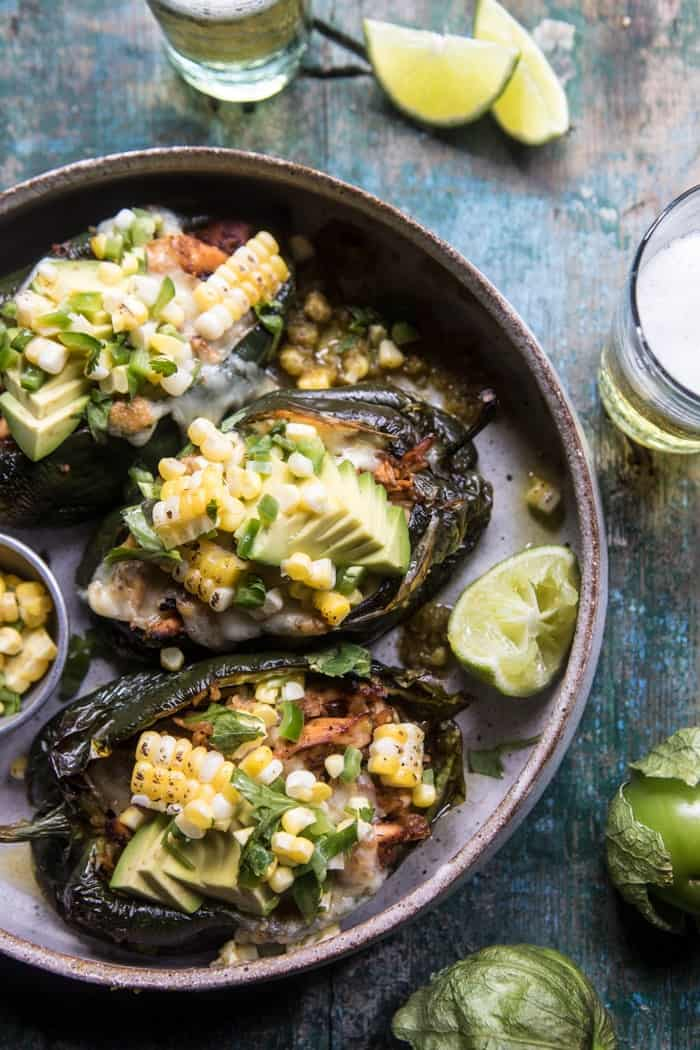
\includegraphics[width=1\textwidth,height=\textheight]{images/lightened-up-salsa-verde-chicken-stuffed-poblano-peppers.jpg}

\textbf{Prep Time:} 20 min \textbar{} \textbf{Cook Time:} 40 min
\textbar{} \textbf{Total Time:} 1 hr

\section{Ingredients}\label{ingredients-61}

\begin{itemize}
\tightlist
\item
  1 pound boneless skinless chicken tenders or small breasts
\item
  2 tablespoons olive oil
\item
  2 teaspoons chili powder
\item
  1 teaspoon smoked paprika
\item
  kosher salt and pepper to taste
\item
  6 poblano peppers
\item
  2 cups homemade or store bought salsa verde
\item
  1 cup cooked brown rice or quinoa
\item
  1/2 cup fresh cilantro, chopped
\item
  2 cups shredded pepper jack
\item
  1 avocado diced or sliced
\item
  2 ears of corns, kernels removed
\item
  1 jalapeno, seeded + chopped
\item
  juice of 1 lime
\item
  1/3 cup fresh cilantro, chopped
\end{itemize}

\section{Instructions}\label{instructions-61}

\begin{enumerate}
\def\labelenumi{\arabic{enumi}.}
\tightlist
\item
  Preheat the oven to 350 degrees F.
\item
  Place the chicken on a baking sheet and rub with the olive oil, chili
  powder, and paprika. Season with salt and pepper. Add the whole
  poblanos to the baking sheet. Transfer to the oven and bake for 20
  minutes or until the chicken is cooked through. Remove the peppers
  from the pan and set aside.
\item
  Shred the chicken with two forks. Add 1/2 cup salsa verde, the rice, 1
  cup cheese, the cilantro, and toss to combine. Pour 1/2 cup of the
  salsa verde onto the bottom of a 9x13 inch baking dish.
\item
  Cut a slit down the length of each poblano pepper. Using your fingers
  remove, and then discard the seeds from each pepper. Stuff the chicken
  mixture inside the peppers and arrange in the the prepared baking
  dish. Pour the remaining salsa verde over top of the peppers and then
  top with the remaining the cheese. Transfer to the oven and bake for
  15-20 minutes, until the cheese has melted. Remove and top with the
  Avocado Corn Salsa.
\end{enumerate}

\bookmarksetup{startatroot}

\chapter{Easy 3 Cup Chicken with
Zucchini.}\label{easy-3-cup-chicken-with-zucchini.}

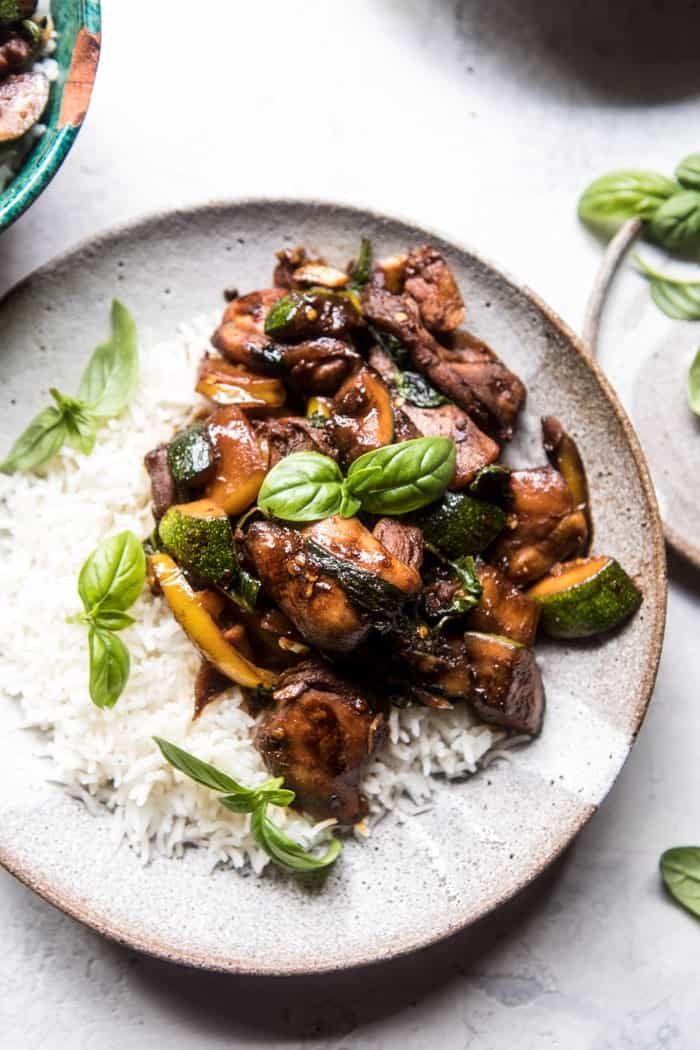
\includegraphics[width=1\textwidth,height=\textheight]{images/easy-3-cup-chicken-with-zucchini-.jpg}

\textbf{Prep Time:} 10 min \textbar{} \textbf{Cook Time:} 20 min
\textbar{} \textbf{Total Time:} 30 min

\section{Ingredients}\label{ingredients-62}

\begin{itemize}
\tightlist
\item
  1/3 cup low sodium soy sauce
\item
  1/3 cup rice vinegar
\item
  4 tablespoons sesame oil
\item
  1 1/2 pounds boneless skinless chicken breasts or thighs, cut in to
  2-3 inch pieces
\item
  1 inch fresh ginger, thinly sliced
\item
  3 cloves garlic, thinly sliced
\item
  1 teaspoon chili flakes
\item
  1 zucchini, chopped
\item
  1 bell pepper, sliced
\item
  1 cup fresh basil
\item
  rice for serving
\end{itemize}

\section{Instructions}\label{instructions-62}

\begin{enumerate}
\def\labelenumi{\arabic{enumi}.}
\tightlist
\item
  In a small bowl, combine the soy sauce, rice vinegar, and 2
  tablespoons sesame oil.
\item
  Heat a large skillet over medium high heat and add the remaining 2
  tablespoons sesame oil. When the oil shimmers, add the chicken and
  cook, stirring occasionally until the chicken is cooked through, about
  8-10 minutes. Add the ginger and garlic, and cook another minute more.
\item
  Pour in the soy sauce/rice vinegar mixture and toss in the zucchini
  and bell pepper. Cook until the sauce thickens and coats the chicken,
  about 5-10 minutes.
\item
  Remove the skillet from the stove and stir in the basil. Serve over
  rice. Enjoy!
\end{enumerate}

\bookmarksetup{startatroot}

\chapter{Freezer Friendly Whole Grain
Waffles}\label{freezer-friendly-whole-grain-waffles}

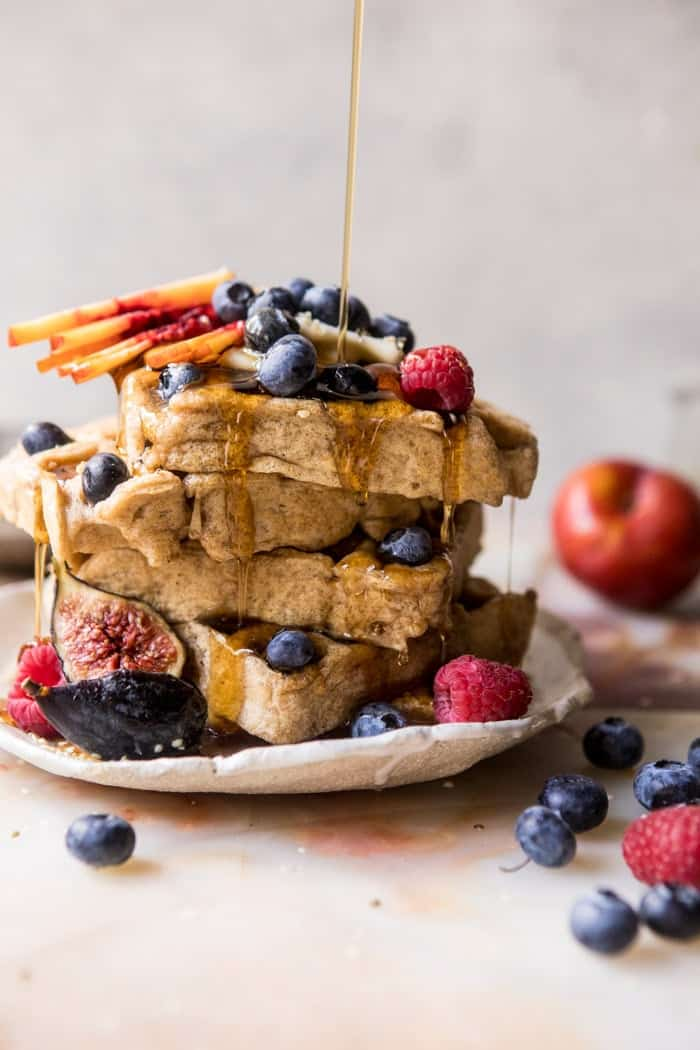
\includegraphics[width=1\textwidth,height=\textheight]{images/freezer-friendly-whole-grain-waffles.jpg}

\textbf{Prep Time:} 15 min \textbar{} \textbf{Cook Time:} 10 min
\textbar{} \textbf{Total Time:} 25 min

\section{Ingredients}\label{ingredients-63}

\begin{itemize}
\tightlist
\item
  2 1/2 cups white whole wheat flour or whole wheat pastry flour
\item
  1/2 cup old fashioned oats
\item
  2 teaspoons baking powder
\item
  1/2 teaspoon cinnamon
\item
  1/2 teaspoon salt
\item
  1 1/2 cups Almond Breeze Unsweetened Original Almondmilk
\item
  2 eggs
\item
  4 tablespoons melted butter
\item
  2 tablespoons honey or brown sugar
\item
  2 teaspoons vanilla extract
\item
  fresh fruit, maple syrup, and whipped cream for serving
\end{itemize}

\section{Instructions}\label{instructions-63}

\begin{enumerate}
\def\labelenumi{\arabic{enumi}.}
\tightlist
\item
  In a large mixing bowl, whisk together the Almondmilk, eggs, melted
  unsalted butter, honey, and vanilla. Add the flour, oats, baking
  powder, cinnamon, and salt and stir until just combined. It's OK if
  the batter is a little lumpy. Allow the batter to sit 5-10 minutes.
\item
  Preheat your waffle iron.
\item
  Cook the waffles according to your waffle iron's directions. Serve
  topped with fresh fruit and maple.
\item
  TO FREEZE: Cool the waffles completely on wire racks. Line a baking
  sheet with parchment paper and place the waffles in one even layer.
  Place another sheet of parchment over the waffles, then arrange
  another layer of waffles over top (see photo). Freeze 2 hours and then
  transfer the waffles to a freezer safe bag. To cook, add the waffles
  to a toaster and toast until warmed through and crisp.
\end{enumerate}

\bookmarksetup{startatroot}

\chapter{Sneaky Zucchini Mac and Cheese with Everything Bagel Chip
Crumbs}\label{sneaky-zucchini-mac-and-cheese-with-everything-bagel-chip-crumbs}

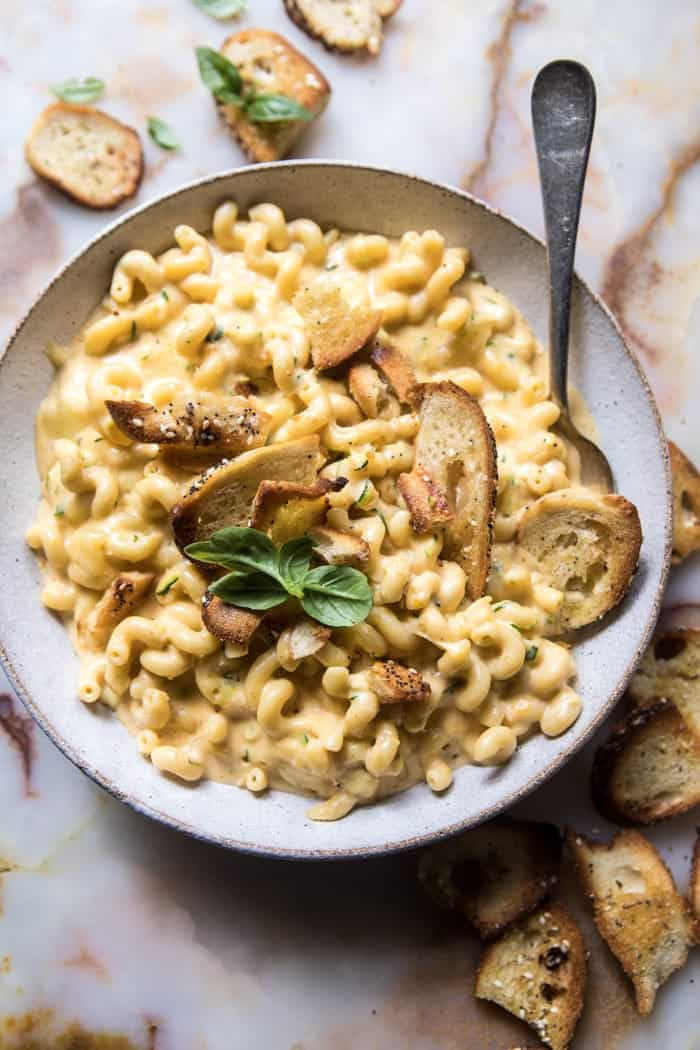
\includegraphics[width=1\textwidth,height=\textheight]{images/sneaky-zucchini-mac-and-cheese-with-everything-bagel-chip-crumbs.jpg}

\textbf{Prep Time:} 15 min \textbar{} \textbf{Cook Time:} 25 min
\textbar{} \textbf{Total Time:} 40 min

\section{Ingredients}\label{ingredients-64}

\begin{itemize}
\tightlist
\item
  3 tablespoons olive oil
\item
  2 everything bagels thinly sliced
\item
  4 tablespoons butter
\item
  1/4 cup all-purpose flour
\item
  3 cups whole milk
\item
  1 pound short cut pasta
\item
  2 medium zucchini, grated
\item
  3 cups shredded sharp cheddar cheese
\item
  1 cup shredded Havarti cheese
\item
  1/4 teaspoon garlic powder
\item
  1/4 teaspoon cayenne pepper
\item
  kosher salt + pepper
\end{itemize}

\section{Instructions}\label{instructions-64}

\begin{enumerate}
\def\labelenumi{\arabic{enumi}.}
\tightlist
\item
  Preheat oven to 350 degrees F. Toss together the bagel pieces, olive
  oil, and a pinch of salt. Transfer to the oven and bake for 10-15
  minutes, stirring halfway through cooking until the bagels are golden
  and crisp. Remove from the oven.
\item
  Meanwhile, melt the butter in a large pot over medium heat. Whisk in
  the flour. Reduce the heat to medium-low and let cook/bubble for 1
  minute. Gradually whisk in the milk, 2 cups water and the pasta. Raise
  the heat up to medium-high and bring the mixture to a low boil, stir
  frequently until the pasta is al dente, about 15 minutes, adding in
  1/4 cup more water as needed until the pasta is al dente. It is
  important to stir the sauce often to insure the pasta is being evenly
  cooked.
\item
  Once the pasta is al dente, stir in the zucchini, all of the cheeses,
  garlic powder, cayenne, salt and pepper. Stir until the cheese is
  fully melted and coats the pasta, about 5-10 minutes.
\item
  Divide the mac and cheese among bowls and top (generously) with
  crushed bagel chips. ENJOY!
\end{enumerate}

\bookmarksetup{startatroot}

\chapter{Homemade Blueberry Nutri Grain
Bars}\label{homemade-blueberry-nutri-grain-bars}

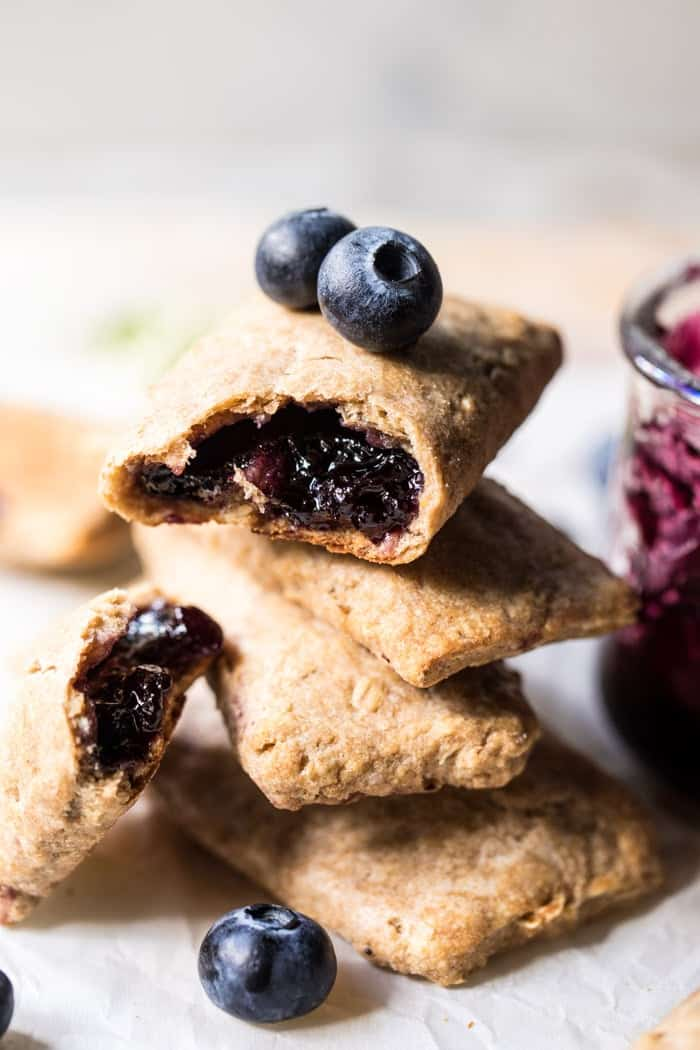
\includegraphics[width=1\textwidth,height=\textheight]{images/homemade-blueberry-nutri-grain-bars.jpg}

\textbf{Prep Time:} 15 min \textbar{} \textbf{Cook Time:} 15 min
\textbar{} \textbf{Total Time:} 30 min

\section{Ingredients}\label{ingredients-65}

\begin{itemize}
\tightlist
\item
  1 cup Bob's Red Mill Whole Wheat Flour
\item
  3/4 cup Bob's Red Mill Old Fashioned Oats
\item
  1/4 teaspoon cinnamon
\item
  1/4 teaspoon kosher salt
\item
  6 tablespoons cold unsalted butter, grated
\item
  2 egg yolks
\item
  2 tablespoons plain greek yogurt
\item
  2 tablespoons honey
\item
  2 teaspoons vanilla
\item
  1 cup blueberry jam, homemade or store-bought
\item
  buttermilk, for brushing
\end{itemize}

\section{Instructions}\label{instructions-65}

\begin{enumerate}
\def\labelenumi{\arabic{enumi}.}
\tightlist
\item
  Preheat the oven to 350 degrees F. In a large bowl, mix the flour,
  oatmeal, cinnamon, and salt together. Add the butter and toss to coat.
  Add the egg yolks, yogurt, honey, and vanilla and mix until combined,
  adding 1 tablespoon of cold water at a time until the dough comes
  together and forms a ball.
\item
  Turn the dough out onto a floured surface. Roll out into a 1/8-inch
  thickness. Cut the dough into about 4'' x 4 1/2'' squares. Place a
  heaping tablespoon of jam down the center of each square, leaving
  about 1/4 inch border. Brush the borders with buttermilk. Fold one
  side up and over the filling and then pinch the dough together at
  either end. Do the same for the other side and use your fingers to
  seal the dough together at the seams. Carefully roll the bar over and
  place the seam side down on a baking sheet lined with parchment paper.
  Repeat with remaining dough.
\item
  Cover the bars and place the baking sheet in the freezer for 10-15
  minutes. Once chilled, brush the tops of the bars lightly with
  buttermilk and transfer to the oven, bake on the middle rack for 15-20
  minutes or until lightly golden brown on top, do not over bake.
\item
  Allow to cool 5-10 minutes, then carefully transfer the bars to a
  glass container with a lid, layering them between pieces of parchment
  paper. This will trap in heat and moisture, and slightly steam the
  bars, ensuring they remain soft. Store in an airtight container for up
  to 3 days or in the fridge for longer. These can also be wrapped in
  plastic wrap and frozen, thaw for 1 hour.
\end{enumerate}

\bookmarksetup{startatroot}

\chapter{Sicilian Style Salmon with Garlic Broccoli and
Tomatoes}\label{sicilian-style-salmon-with-garlic-broccoli-and-tomatoes}

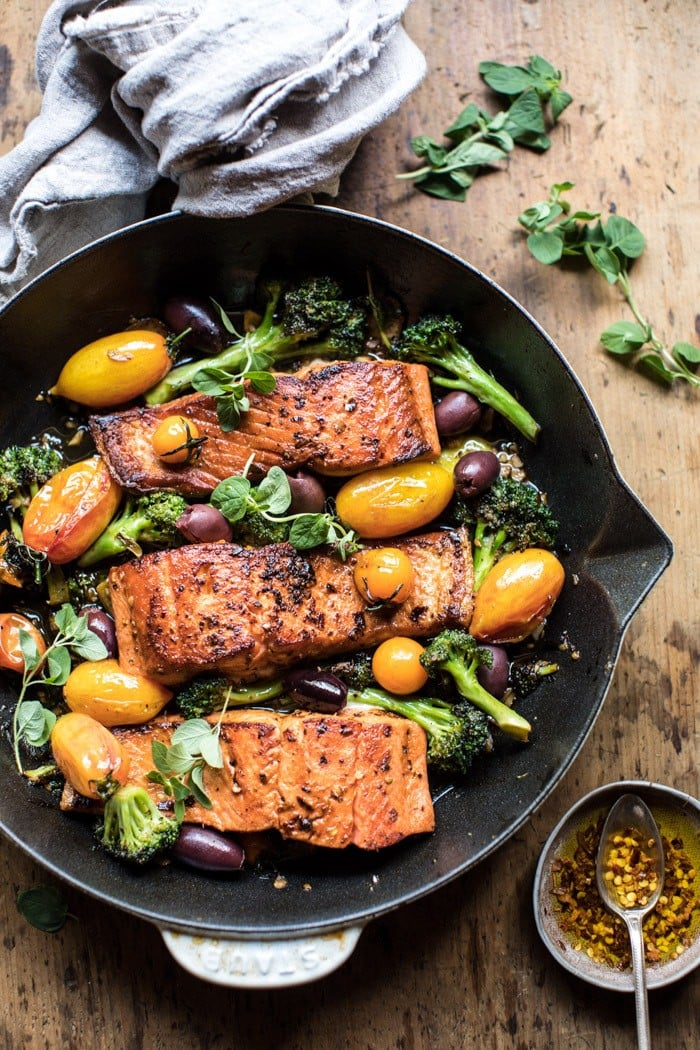
\includegraphics[width=1\textwidth,height=\textheight]{images/sicilian-style-salmon-with-garlic-broccoli-and-tomatoes.jpg}

\textbf{Prep Time:} 10 min \textbar{} \textbf{Cook Time:} 15 min
\textbar{} \textbf{Total Time:} 25 min

\section{Ingredients}\label{ingredients-66}

\begin{itemize}
\tightlist
\item
  4 salmon fillets
\item
  extra virgin olive oil, for rubbing
\item
  juice from 1 lemon
\item
  1 teaspoon red pepper flakes
\item
  1 teaspoon paprika
\item
  kosher salt and pepper
\item
  1 large head of broccoli, cut into florets
\item
  1 cup cherry tomatoes
\item
  2 cloves garlic, minced or grated
\item
  2 tablespoons chopped fresh oregano
\item
  zest from 1 lemon
\item
  splash of white wine
\item
  1/2 cup pitted kalamata olives
\end{itemize}

\section{Instructions}\label{instructions-66}

\begin{enumerate}
\def\labelenumi{\arabic{enumi}.}
\tightlist
\item
  Heat a drizzle of olive oil in a large skillet over medium high heat.
\item
  Rub the salmon all over with olive oil and lemon juice. Sprinkle with
  chili flakes, paprika, salt, and pepper. Place flesh side down in the
  skillet and sear until crisp and just beginning to caramelize, about
  2-3 minutes. Flip and cook 1 minute more or until your desired
  doneness is reached. Remove the salmon from the skillet.
\item
  Add another drizzle of oil to the pan, add the broccoli and cook until
  tender, about 5 minutes. Add the tomatoes, garlic, oregano, lemon
  zest, salt and pepper and cook until the tomatoes begin to burst,
  about 5 minutes. Remove from the heat and add a splash of wine to
  create a sauce. Add the olives and slide the salmon back into the
  skillet to warm throughout.
\item
  Serve the salmon with a side of veggies and any sauce left in the
  skillet. Garnish with fresh oregano.
\end{enumerate}

\bookmarksetup{startatroot}

\chapter{PB\&J Oat Streusel Muffins}\label{pbj-oat-streusel-muffins}

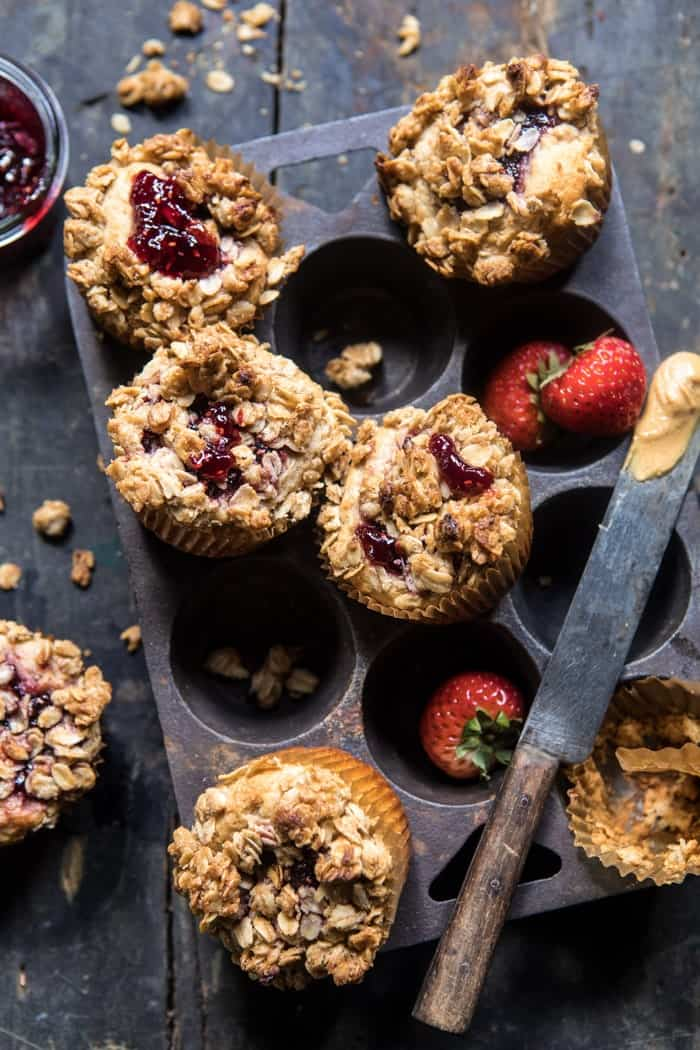
\includegraphics[width=1\textwidth,height=\textheight]{images/pb-j-oat-streusel-muffins.jpg}

\textbf{Prep Time:} 20 min \textbar{} \textbf{Cook Time:} 20 min
\textbar{} \textbf{Total Time:} 40 min

\section{Ingredients}\label{ingredients-67}

\begin{itemize}
\tightlist
\item
  1/2 cup melted coconut oil or butter
\item
  1/2 cup honey
\item
  2 teaspoons vanilla extract
\item
  1 cup buttermilk
\item
  1 cup plain greek yogurt
\item
  2 eggs
\item
  1 1/2 cups all-purpose flour
\item
  1 cup white whole wheat flour
\item
  2 teaspoons baking powder
\item
  1/2 teaspoon kosher salt
\item
  1/2 cup creamy peanut butter
\item
  1/2 cup raspberry or strawberry jam
\item
  1 1/2 cups old fashioned oats
\item
  3 tablespoons all purpose flour
\item
  2 tablespoons brown sugar
\item
  1 teaspoon cinnamon
\item
  6 tablespoons softened salted butter, cubed
\end{itemize}

\section{Instructions}\label{instructions-67}

\begin{enumerate}
\def\labelenumi{\arabic{enumi}.}
\tightlist
\item
  Preheat the oven to 350 degrees F. Line 18 muffin tins with paper
  liners.
\item
  In a large mixing bowl, whisk together the oil, honey, vanilla,
  buttermilk, greek yogurt, and eggs until smooth. Add the flour, whole
  wheat flour, baking powder, and salt and mix until just combined.
\item
  Gently fold the peanut butter into the batter, being careful not to
  over mix. Remember, you're going for a peanut butter swirl look.
\item
  Divide the batter evenly among the prepared muffins tins. Using a
  spoon, make a teaspoon side indent in the middle of each muffin and
  spoon the jam into each.
\item
  To make the streusel. Combine the oats, flour, brown sugar, cinnamon
  and salt in a medium size mixing bowl. Add the butter and use your
  hands to work the butter into the dry ingredients until everything is
  moist and clumps together. Sprinkle the topping over muffins. Transfer
  to the oven and bake for 20-25 minutes or until a toothpick inserted
  into the center comes out clean. Enjoy!!
\end{enumerate}

\bookmarksetup{startatroot}

\chapter{Opened Faced Tomato and Goat Cheese Sandwich with Hot Bacon
Vinaigrette}\label{opened-faced-tomato-and-goat-cheese-sandwich-with-hot-bacon-vinaigrette}

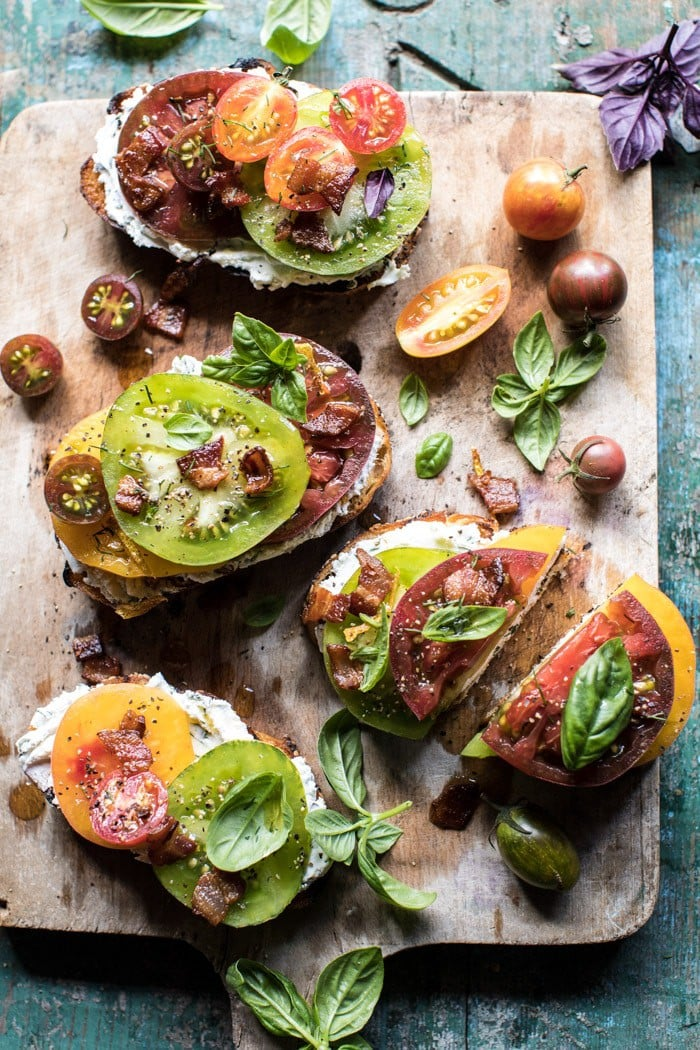
\includegraphics[width=1\textwidth,height=\textheight]{images/opened-faced-tomato-and-goat-cheese-sandwich-with-hot-bacon-vinaigrette.jpg}

\textbf{Prep Time:} 10 min \textbar{} \textbf{Cook Time:} 5 min
\textbar{} \textbf{Total Time:} 15 min

\section{Ingredients}\label{ingredients-68}

\begin{itemize}
\tightlist
\item
  6-8 ounces goat cheese
\item
  2 teaspoons chopped fresh dill
\item
  2 teaspoons chopped fresh basil, plus more for serving
\item
  2 teaspoons lemon juice
\item
  kosher salt and pepper
\item
  6 slices whole grain or sourdough bread
\item
  3 heirloom tomatoes, sliced
\item
  6 slices bacon, chopped
\item
  2 tablespoons red wine vinegar
\item
  3 tablespoons extra virgin olive oil
\item
  1 pinch crushed red pepper flakes
\item
  1 pinch each salt and pepper
\end{itemize}

\section{Instructions}\label{instructions-68}

\begin{enumerate}
\def\labelenumi{\arabic{enumi}.}
\tightlist
\item
  Preheat your grill to high heat or preheat your oven to 400 degrees F.
\item
  In a medium bowl, stir together the goat cheese, dill, basil, lemon
  juice and a pinch each of salt and pepper.
\item
  Place the bread on a baking sheet and drizzle with olive oil on both
  sides, season with salt and pepper. Place the bread on the grill and
  grill both for about 2-3 minutes per side or until lightly chard.
  Remove from the grill.
\item
  Spread the goat cheese over the bread and top with tomatoes. Season
  the tomatoes lightly with salt and pepper.
\item
  Heat a large skillet over medium high heat and cook the bacon until
  crisp. Drain off all but 1 tablespoon of bacon grease. To the bacon,
  add the vinegar, olive oil, and a pinch each of red pepper, salt, and
  pepper. Drizzle the warm vinaigrette over the tomatoes. Top with
  basil. EAT!
\end{enumerate}

\bookmarksetup{startatroot}

\chapter{Bourbon Cherry Old
Fashioned}\label{bourbon-cherry-old-fashioned}

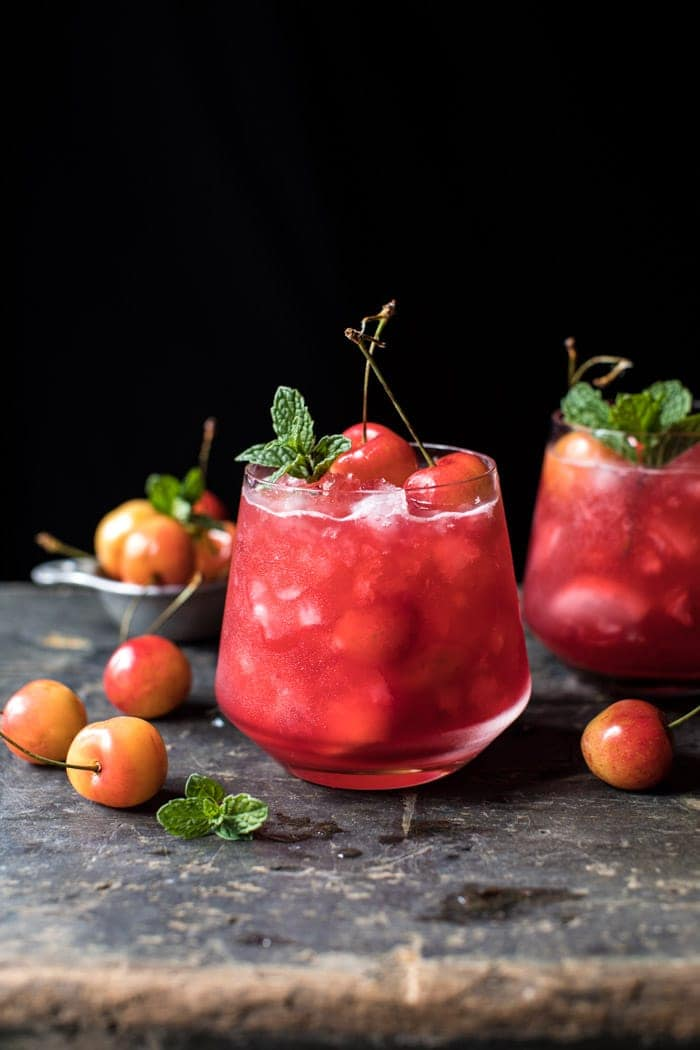
\includegraphics[width=1\textwidth,height=\textheight]{images/bourbon-cherry-old-fashioned.jpg}

\textbf{Prep Time:} 5 min \textbar{} \textbf{Cook Time:} \textbar{}
\textbf{Total Time:} 5 min

\section{Ingredients}\label{ingredients-69}

\begin{itemize}
\tightlist
\item
  4-6 fresh cherries, pitted
\item
  juice from half a lime
\item
  dash of orange bitters
\item
  1-2 tablespoons honey
\item
  2 ounces bourbon, more or less to taste
\item
  fresh mint and cherries for garnish
\end{itemize}

\section{Instructions}\label{instructions-69}

\begin{enumerate}
\def\labelenumi{\arabic{enumi}.}
\tightlist
\item
  Muddle the cherries, lime juice, orange bitters, and honey in a
  cocktail shaker or glass jar until the cherries are well mashed and
  have released their juices. Add the bourbon and shake to combine.
\item
  Strain (or not, I leave my cherries in!) into a cocktail glass filled
  with ice. If desired top with sparking water. Garnish with mint and
  cherries. DRINK! ?
\end{enumerate}

\bookmarksetup{startatroot}

\chapter{Blackberry Lavender White Chocolate
Clafoutis}\label{blackberry-lavender-white-chocolate-clafoutis}

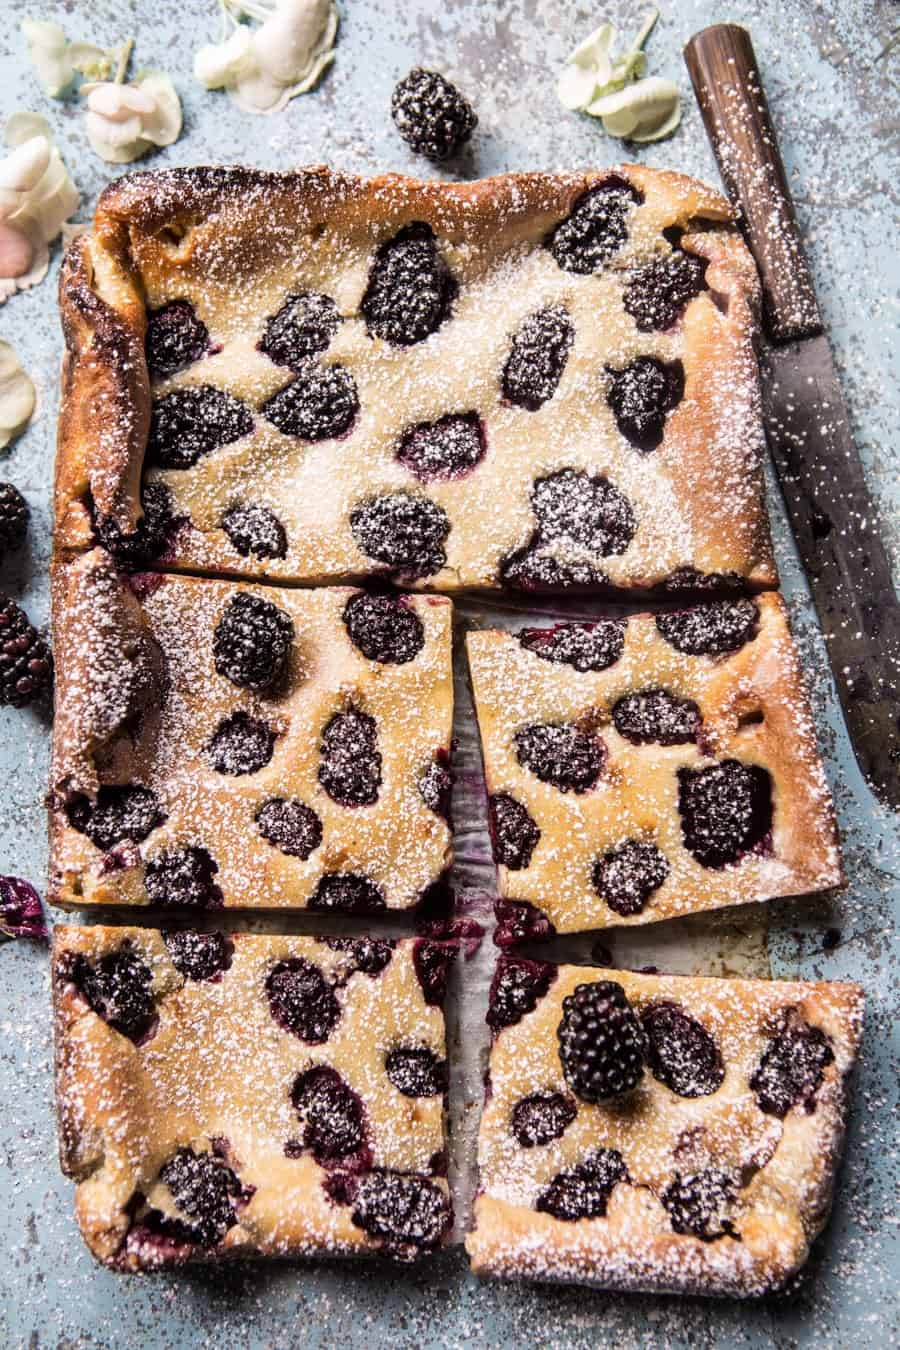
\includegraphics[width=1\textwidth,height=\textheight]{images/blackberry-lavender-white-chocolate-clafoutis.jpg}

\textbf{Prep Time:} 10 min \textbar{} \textbf{Cook Time:} 30 min
\textbar{} \textbf{Total Time:} 40 min

\section{Ingredients}\label{ingredients-70}

\begin{itemize}
\tightlist
\item
  butter, for greasing
\item
  1/2 cup granulated sugar
\item
  1 tablespoon dried lavender ((use another tablespoon for more flavor))
\item
  1 1/4 cups whole milk
\item
  3 large eggs
\item
  2 teaspoons vanilla extract
\item
  1 pinch kosher salt
\item
  1 cup all purpose flour
\item
  2 cups fresh blackberries
\item
  1/3 cup white chocolate chips
\item
  powdered sugar, for dusting
\end{itemize}

\section{Instructions}\label{instructions-70}

\begin{enumerate}
\def\labelenumi{\arabic{enumi}.}
\tightlist
\item
  Preheat the oven to 350 degrees F. Grease an 10 inch baking dish with
  softened butter.
\item
  In a blender or food processor, combine the sugar and lavender and
  pulse until ground. Remove half of the lavender sugar and set aside.
  To the blender, add the milk, eggs, vanilla, salt and flour. Blend
  until completely smooth. Pour the batter into the prepared baking
  dish. Sprinkle over the blackberries and white chocolate. Sprinkle the
  remaining lavender sugar evenly over top.
\item
  Bake in the center of the oven for 30 minutes or until golden and
  puffed on the edges. The clafoutis will sink as it cools. Dust with
  powdered sugar and serve warm.
\end{enumerate}

\bookmarksetup{startatroot}

\chapter{Thai Coconut Mussels with Garlic Lemongrass
Toast}\label{thai-coconut-mussels-with-garlic-lemongrass-toast}

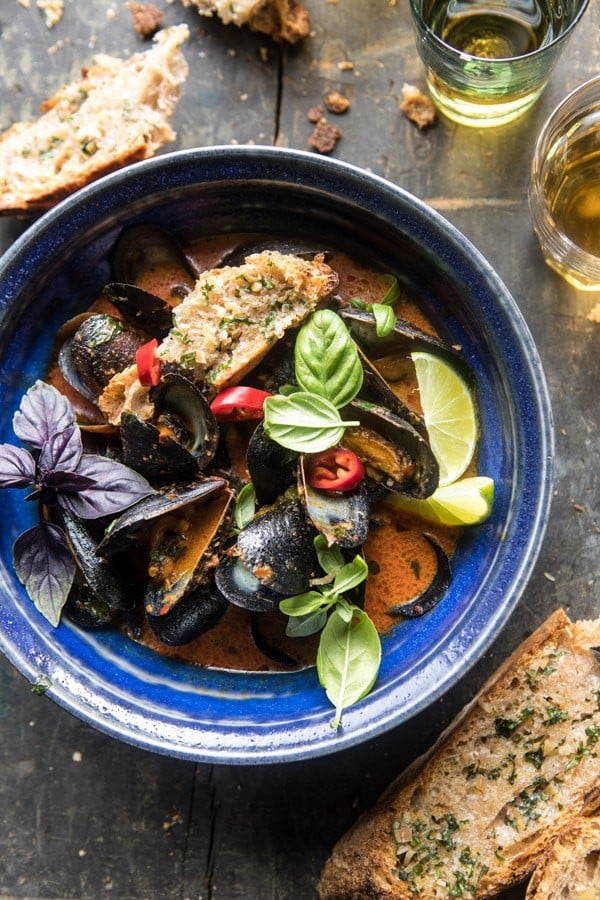
\includegraphics[width=1\textwidth,height=\textheight]{images/thai-coconut-mussels-with-garlic-lemongrass-toast.jpg}

\textbf{Prep Time:} 10 min \textbar{} \textbf{Cook Time:} 15 min
\textbar{} \textbf{Total Time:} 25 min

\section{Ingredients}\label{ingredients-71}

\begin{itemize}
\tightlist
\item
  2 1/2 pounds black mussels, beards removed and scrubbed clean
\item
  4 tablespoons Land O Lakes® Salted Butter
\item
  1/4 cup Thai red curry paste
\item
  1 14 ounce can full-fat coconut milk
\item
  1/2 cup white wine
\item
  kosher salt and pepper
\item
  1/4 cup fresh basil, roughly torn, plus more for serving
\item
  fresh limes and chiles, for serving
\item
  4 tablespoons Land O Lakes® Salted Butter
\item
  1 tablespoon finely chopped lemongrass
\item
  2 cloves garlic, minced or grated
\item
  1/4 cup fresh basil, chopped
\item
  1 sourdough baguette sliced
\end{itemize}

\section{Instructions}\label{instructions-71}

\begin{enumerate}
\def\labelenumi{\arabic{enumi}.}
\tightlist
\item
  In a large skillet, melt the butter over medium heat. Add the curry
  paste and cook for 1 minute. Stir in the coconut milk, wine, and a
  pinch each of salt and pepper. Bring the mixture to a simmer and add
  the mussels. Cover and cook for 4-5 minutes, shaking the pan
  occasionally until the mussels have all opened. Discard any mussels
  that don’t open. Stir in the basil.
\item
  Meanwhile, make the toast. Preheat the oven to 425 degrees F.
\item
  In a small bowl, combine the butter, lemongrass, garlic, basil, and a
  pinch of salt. Spread the butter over each piece of bread and place on
  a baking sheet. Transfer to the oven and cook for 8-10 minutes or
  until the bread is toasted.
\item
  Serve the mussels warm with basil, limes and chiles. Serve the toast
  on the side for dipping. Enjoy!
\end{enumerate}

\bookmarksetup{startatroot}

\chapter{Raspberry Ginger Stone Fruit
Galette}\label{raspberry-ginger-stone-fruit-galette}

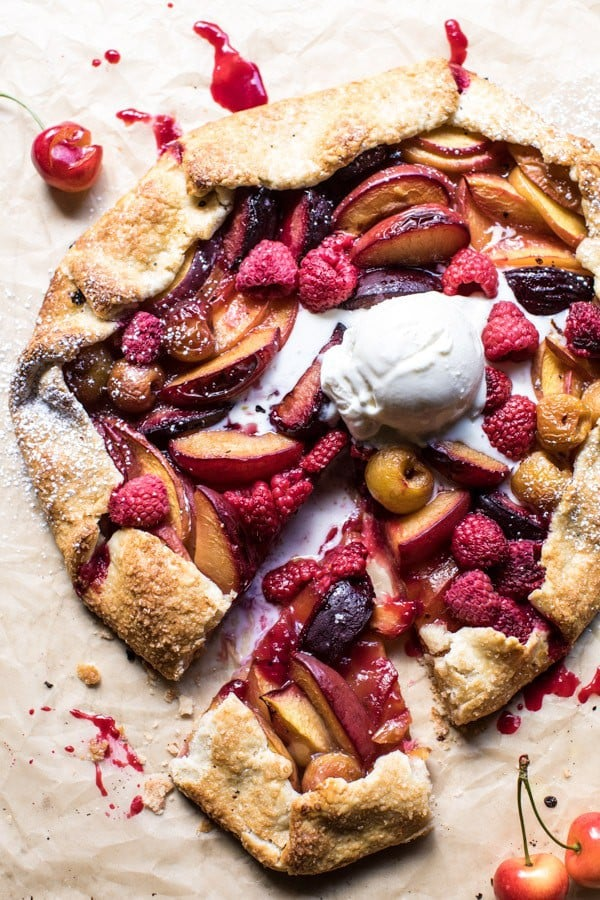
\includegraphics[width=1\textwidth,height=\textheight]{images/raspberry-ginger-stone-fruit-galette.jpg}

\textbf{Prep Time:} 20 min \textbar{} \textbf{Cook Time:} 40 min
\textbar{} \textbf{Total Time:} 1 hr

\section{Ingredients}\label{ingredients-72}

\begin{itemize}
\tightlist
\item
  1 1/2 cups flour
\item
  1/2 teaspoon kosher salt
\item
  8 tablespoons unsalted butter, cold + cut into 1/2 inch cubes
\item
  3-6 tablespoons cold buttermilk or water
\item
  3 cups sliced stone fruit
\item
  1/4 cup brown sugar
\item
  1 inch fresh knob fresh ginger, grated
\item
  1 tablespoon bourbon ((optional))
\item
  1 tablespoon cornstarch
\item
  juice from 1/2 a lemon
\item
  1 1/2 cups fresh raspberries
\item
  1 egg
\item
  coarse sugar for sprinkling
\end{itemize}

\section{Instructions}\label{instructions-72}

\begin{enumerate}
\def\labelenumi{\arabic{enumi}.}
\tightlist
\item
  Place the all-purpose flour, and salt in a large bowl. Add the butter
  and then use your fingers to break the butter into the flour until the
  mixture is the size of small peas. Add 3 tablespoons buttermilk and
  mix with a wooden spoon, drizzling in more as needed (no more than 1
  tablespoon at a time), until dough just comes together (a few dry
  spots are ok). Gently knead dough on a lightly floured surface until
  no dry spots remain, about 1 minute. At this point you can cover the
  dough and place it in the fridge while you prepare the filling, or for
  up to one week.
\item
  In a bowl, toss together the stone fruit, brown sugar, ginger, bourbon
  (if using), cornstarch and lemon juice.
\item
  Now grab your dough from the fridge. Flour your work surface again and
  roll the dough to about 1/8-inch thick. Transfer to a baking sheet
  lined with parchment paper. Arrange the fruit over the dough in an
  even layer, leaving a 1 inch border around the dough. Pour any
  remaining juices left in the bowl over the fruit. Sprinkle the
  raspberries over top. Fold the edges of the dough over the filling.
  Brush the crust with the beaten egg and sprinkle the coarse sugar over
  the dough.
\item
  Place the galette in the fridge for 15 minutes or until ready to bake.
\item
  Preheat the oven to 400 degrees F. Bake the galette for 45-50 minutes
  or until the crust is golden and the fruit is soft and caramelized.
  Allow to cool slightly. Serve warm or at room temperature with a large
  scoop of ice cream.
\end{enumerate}

\bookmarksetup{startatroot}

\chapter{Brown Sugar Oatmeal Cookie, Cookie Dough Ice Cream
Sandwiches}\label{brown-sugar-oatmeal-cookie-cookie-dough-ice-cream-sandwiches}

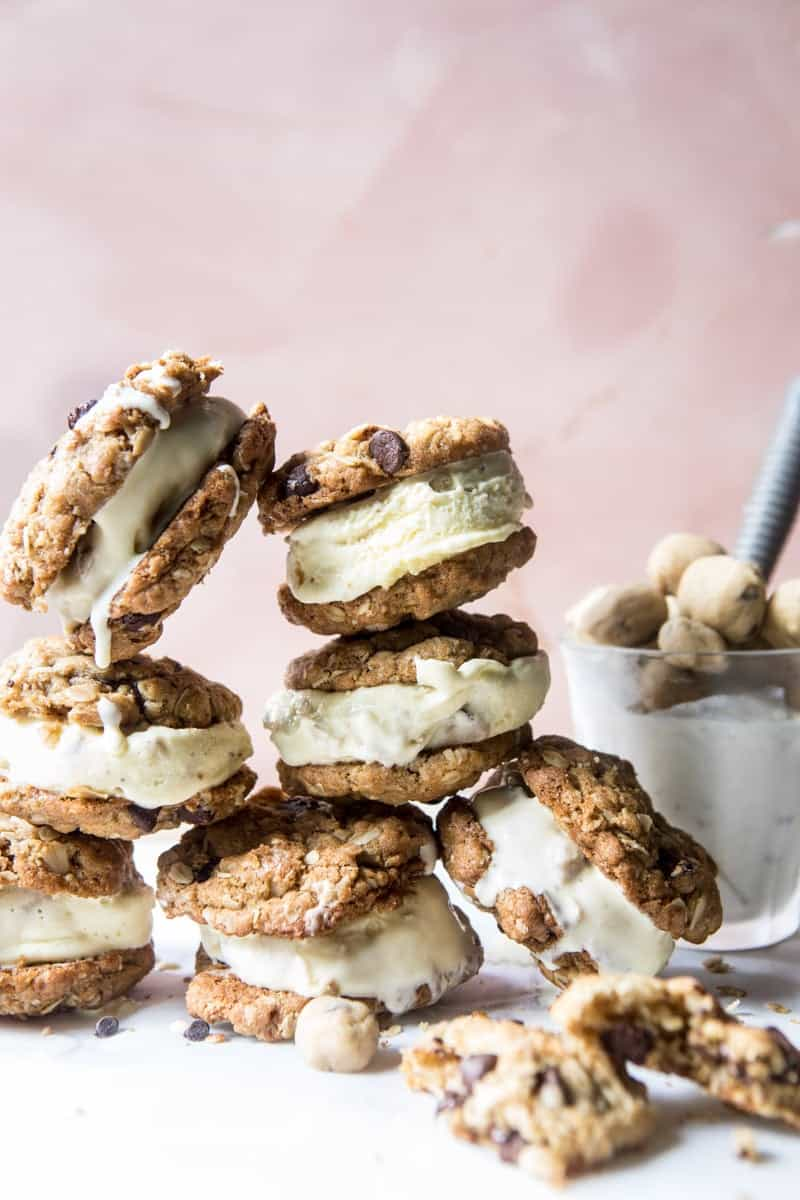
\includegraphics[width=1\textwidth,height=\textheight]{images/brown-sugar-oatmeal-cookie-cookie-dough-ice-cream-sandwiches.jpg}

\textbf{Prep Time:} 30 min \textbar{} \textbf{Cook Time:} 30 min
\textbar{} \textbf{Total Time:} 1 hr

\section{Ingredients}\label{ingredients-73}

\begin{itemize}
\tightlist
\item
  5 large egg yolks
\item
  3/4 cup granulated sugar
\item
  3 cups whole milk
\item
  2 teaspoons vanilla
\item
  1/4 teaspoon flaky sea salt
\item
  1 stick (1/2 cup) salted butter
\item
  1/3 cup light brown sugar
\item
  1/4 cup granulated sugar
\item
  1 pasteurized egg
\item
  2 teaspoons vanilla
\item
  1 3/4 cups all-purpose flour
\item
  1 cup mini semi-sweet chocolate chips
\item
  1 3/4 cups old fashioned oats
\item
  1 cup all-purpose flour
\item
  1 cup packed light brown sugar
\item
  1/2 teaspoon baking soda
\item
  1/2 teaspoon salt
\item
  1/2 cup canola oil or melted coconut oil
\item
  1 large egg
\item
  2 teaspoons vanilla extract
\item
  1 cup semi-sweet chocolate chips
\end{itemize}

\section{Instructions}\label{instructions-73}

\begin{enumerate}
\def\labelenumi{\arabic{enumi}.}
\tightlist
\item
  In a medium size pot, whisk together the egg yolks and sugar until the
  yolks are pale yellow in color. Add the milk, vanilla, and sea salt.
  Set the pot over medium high heat. Bring the mixture to a low boil.
  Cook, stirring consistently, until the mixture thickens and easily
  coats the back of a wooden spoon, about 8-10 minutes. Once thickened
  remove from the heat.
\item
  Place a fine-mesh sieve (strainer) over a large heatproof bowl and
  immediately strain the custard into the bowl. Cool slightly, cover and
  place in the fridge for 4 hours or overnight.
\item
  To make the cookie dough. In a large bowl, beat together the butter,
  brown sugar, and sugar until combined. Add the egg and vanilla and
  beat until combined and creamy. Add the flour and salt, beat until
  combined. Stir in the chocolate chips. Spread the cookie dough in an
  even layer on a parchment lined baking sheet. Freeze 20-30 minutes and
  then roughly chop the cookie dough into small, bite size pieces.
\item
  To make the oatmeal Cookies. Preheat the oven to 350 degrees F.
\item
  In a large bowl beat together the oatmeal, flour, brown sugar, baking
  soda, salt, canola oil, egg, and vanilla until the dough is moist and
  all the ingredients are combined. The dough will be crumbly. Mix in
  the chocolate chips.
\item
  Using your hands clump together a tablespoon of dough. Use you hands
  to really squeeze the dough into a ball. Place on a parchment lined
  baking sheet. Repeat with remaining dough.
\item
  Bake for 12-15 minutes or until set and golden. Let cool completely.
\item
  Churn the ice cream in an ice cream maker according to the
  manufacturer’s instructions. During the last few minutes of churning,
  add the cookie dough pieces.
\item
  Using an ice cream scoop, scoop 1 scoop of ice cream on to half of the
  cookies. Sandwich with the remaining cookies, gently pushing down.
  Transfer to the freezer and freeze for 4-6 hours or until firm (or eat
  now!). Remove 5-10 minutes before eating to soften. Enjoy!
\end{enumerate}

\bookmarksetup{startatroot}

\chapter{Rainbow Thai Basil Noodle Salad with Sesame
Vinaigrette}\label{rainbow-thai-basil-noodle-salad-with-sesame-vinaigrette}

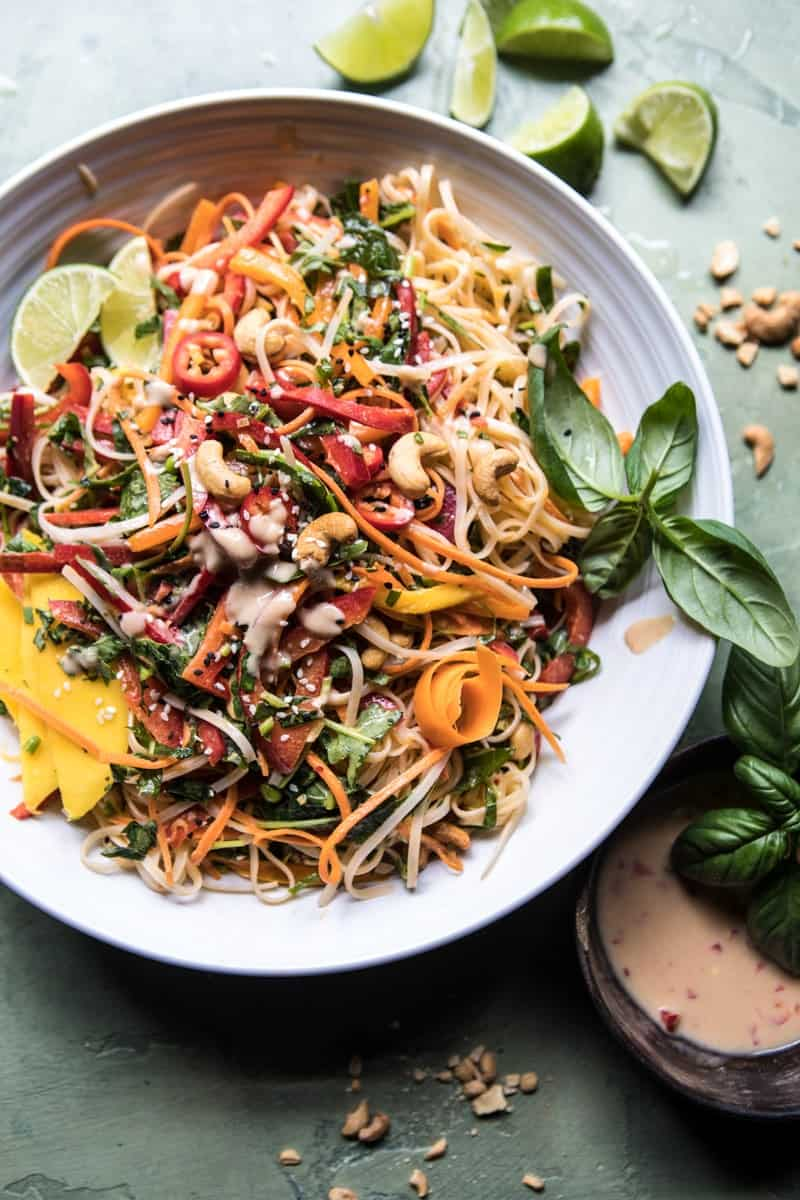
\includegraphics[width=1\textwidth,height=\textheight]{images/rainbow-thai-basil-noodle-salad-with-sesame-vinaigrette.jpg}

\textbf{Prep Time:} 15 min \textbar{} \textbf{Cook Time:} 5 min
\textbar{} \textbf{Total Time:} 20 min

\section{Ingredients}\label{ingredients-74}

\begin{itemize}
\tightlist
\item
  1/3 cup Simple Truth Tahini (sesame seed paste)
\item
  2 tablespoons honey
\item
  juice and zest of 1 lime
\item
  2 tablespoons fish sauce
\item
  1 clove garlic, minced or grated
\item
  1 tablespoon fresh ginger, grated
\item
  1 (8 ounce box) rice noodles
\item
  4 cups baby kale, finely chopped
\item
  1 (16 ounce bag) frozen shelled edamame, thawed
\item
  3 carrots, shredded or chopped
\item
  2 bell peppers (red, yellow and or orange), sliced thin
\item
  1 cup fresh or frozen mango, chopped into chunks
\item
  2 stalks lemongrass, finely chopped
\item
  4 green onions chopped
\item
  3/4 cup fresh basil, and cilantro
\item
  sliced fresno peppers, sesame seeds and roasted cashews, for topping
\end{itemize}

\section{Instructions}\label{instructions-74}

\begin{enumerate}
\def\labelenumi{\arabic{enumi}.}
\tightlist
\item
  To make the vinaigrette, combine the tahini, honey, lime juice, lime
  zest, fish sauce, garlic, and ginger in a small mason jar. Seal the
  jar and shake until the vinaigrette is combined.
\item
  Cook the rice noodle according to package directions. Drain and rinse
  under cold water. Add the noodles to a large salad bowl and toss
  together with the baby kale, edamame, carrots, bell peppers,
  lemongrass, green onions, herbs, and sesame seeds. Drizzle with the
  the vinaigrette and toss well to combine. Serve the salad warm or
  cold.
\end{enumerate}

\bookmarksetup{startatroot}

\chapter{Simple Coconut Mango Chicken and Broccoli
Curry}\label{simple-coconut-mango-chicken-and-broccoli-curry}

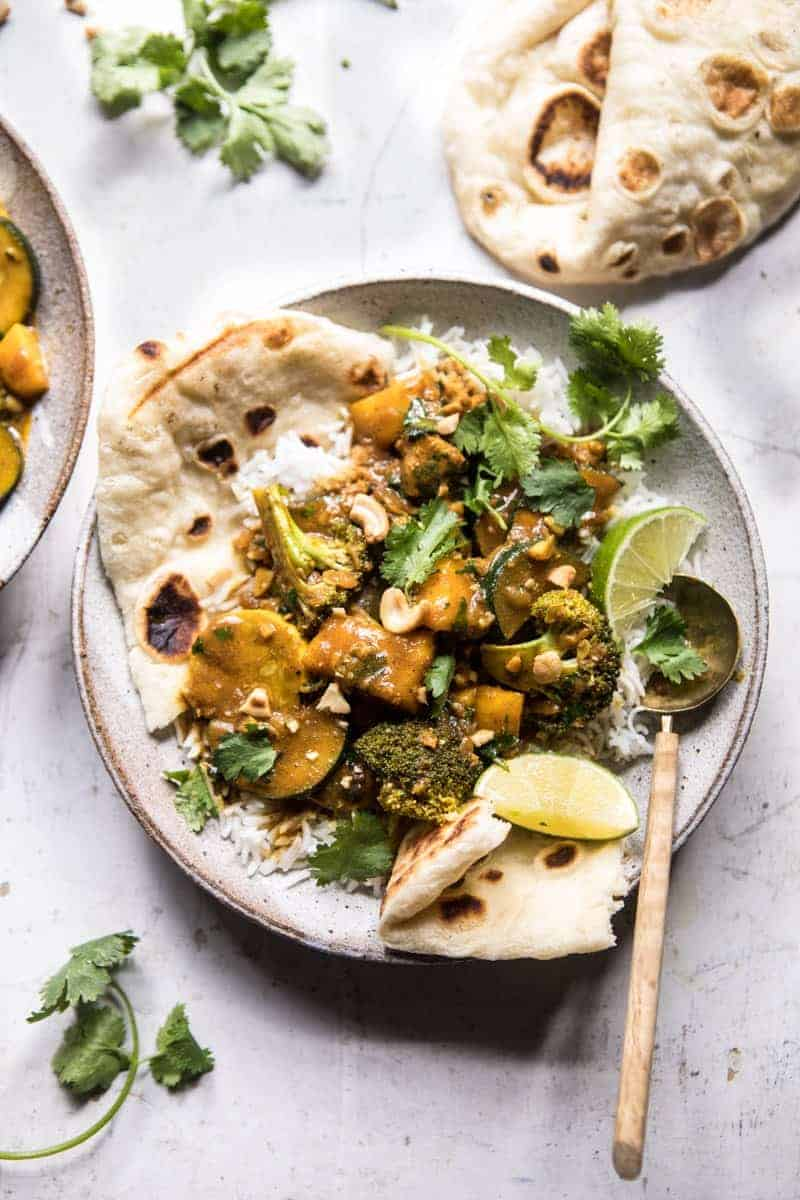
\includegraphics[width=1\textwidth,height=\textheight]{images/simple-coconut-mango-chicken-and-broccoli-curry.jpg}

\textbf{Prep Time:} 10 min \textbar{} \textbf{Cook Time:} 20 min
\textbar{} \textbf{Total Time:} 30 min

\section{Ingredients}\label{ingredients-75}

\begin{itemize}
\tightlist
\item
  2 tablespoons ghee or coconut oil
\item
  1 small sweet onion, diced
\item
  1 1/2 pounds boneless skinless chicken breast, cubed
\item
  1 rounded tablespoon yellow curry powder
\item
  1 teaspoon cayenne pepper, or to taste
\item
  kosher salt and pepper
\item
  4 cloves garlic, minced or grated
\item
  1 inch piece ginger, grated
\item
  2 medium summer squash and or zucchini, sliced into rounds
\item
  1 head broccoli, cut into florets
\item
  1 14 ounce can full fat coconut milk
\item
  1/2 cup fresh cilantro, chopped
\item
  1 mango, diced
\item
  juice + zest of lime
\item
  rice, fresh naan, and roasted cashews, for serving
\end{itemize}

\section{Instructions}\label{instructions-75}

\begin{enumerate}
\def\labelenumi{\arabic{enumi}.}
\tightlist
\item
  Melt the ghee in a large skillet over medium heat. Add the onion and
  season with salt. Cook, stirring occasionally until the onion is
  golden, about 5-8 minutes.
\item
  Add the chicken, curry powder, cayenne and a pinch each of salt and
  pepper. Cook 5 minutes or until the chicken is browned. Add the garlic
  add ginger and cook another minute. Add the zucchini and summer squash
  and cook 2 minutes more. Pour in the coconut milk and add the
  broccoli. Bring the curry to a simmer and cook for 10 minutes or until
  the sauce has thickened slightly and the broccoli is tender.
\item
  Remove from the heat and stir in the cilantro, mango, lime juice and
  zest. Serve the curry over a bed of rice with fresh naan. Top with
  cashews. Enjoy!
\end{enumerate}

\bookmarksetup{startatroot}

\chapter{Frozen Cantaloupe
Margaritas}\label{frozen-cantaloupe-margaritas}

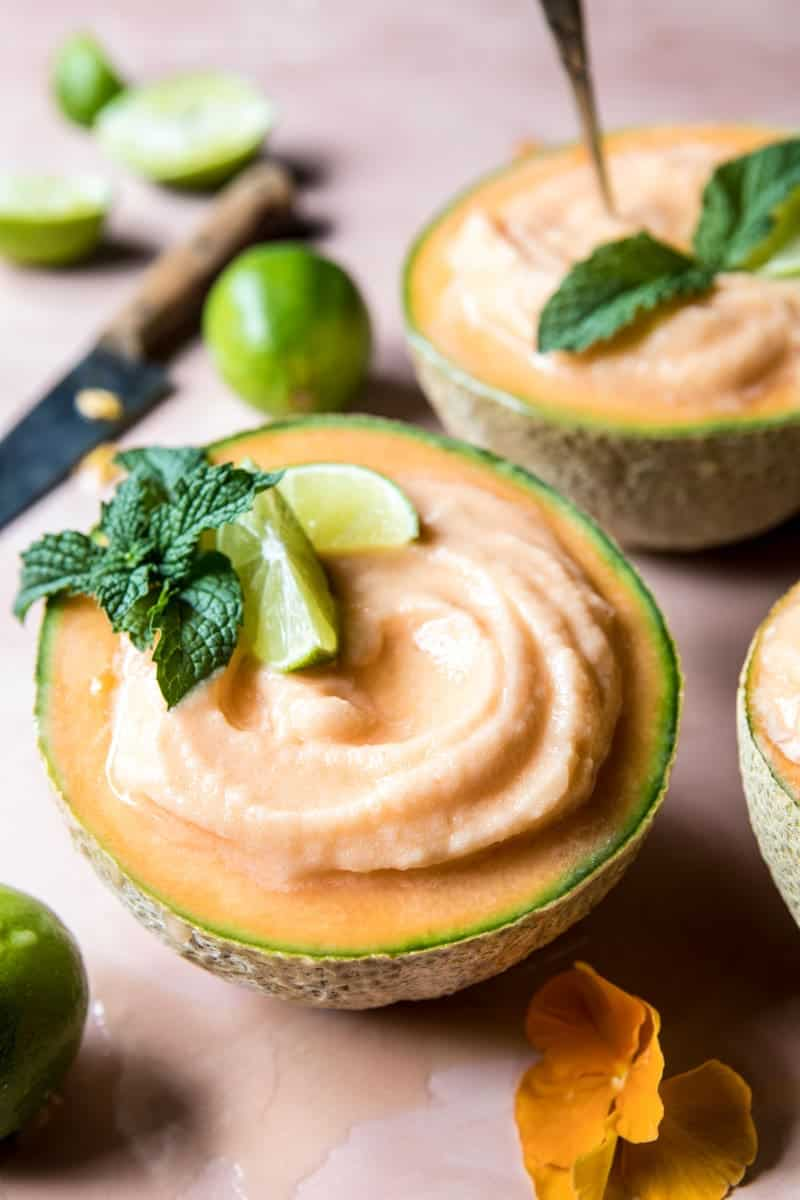
\includegraphics[width=1\textwidth,height=\textheight]{images/frozen-cantaloupe-margaritas.jpg}

\textbf{Prep Time:} 10 min \textbar{} \textbf{Cook Time:} \textbar{}
\textbf{Total Time:} 10 min

\section{Ingredients}\label{ingredients-76}

\begin{itemize}
\tightlist
\item
  2 cups frozen cantaloupe chunks ((freeze chunks for at least 1-2
  hours))
\item
  1/2 cup unsweetened coconut milk
\item
  1/4 cup sliver tequila
\item
  1/4 cup lime juice
\item
  2 tablespoons Cointreau
\item
  1-2 tablespoons agave or honey, to taste
\item
  salt, for the rims ((optional))
\end{itemize}

\section{Instructions}\label{instructions-76}

\begin{enumerate}
\def\labelenumi{\arabic{enumi}.}
\tightlist
\item
  Slice a thin piece of rind off both ends of cantaloupe so that it can
  stand upright. Cut in half horizontally and remove seeds. Scoop out
  flesh and set aside, save cantaloupe halves.
\item
  In a blender, combine the cantaloupe, coconut milk, tequila, lime
  juice, Cointreau and agave, pulse until smooth. If needed, add ice to
  get a slushy consistency. Divide between cantaloupe bowls (halves) and
  drink!
\end{enumerate}

\bookmarksetup{startatroot}

\chapter{Mixed Berry Almond
Croissants}\label{mixed-berry-almond-croissants}

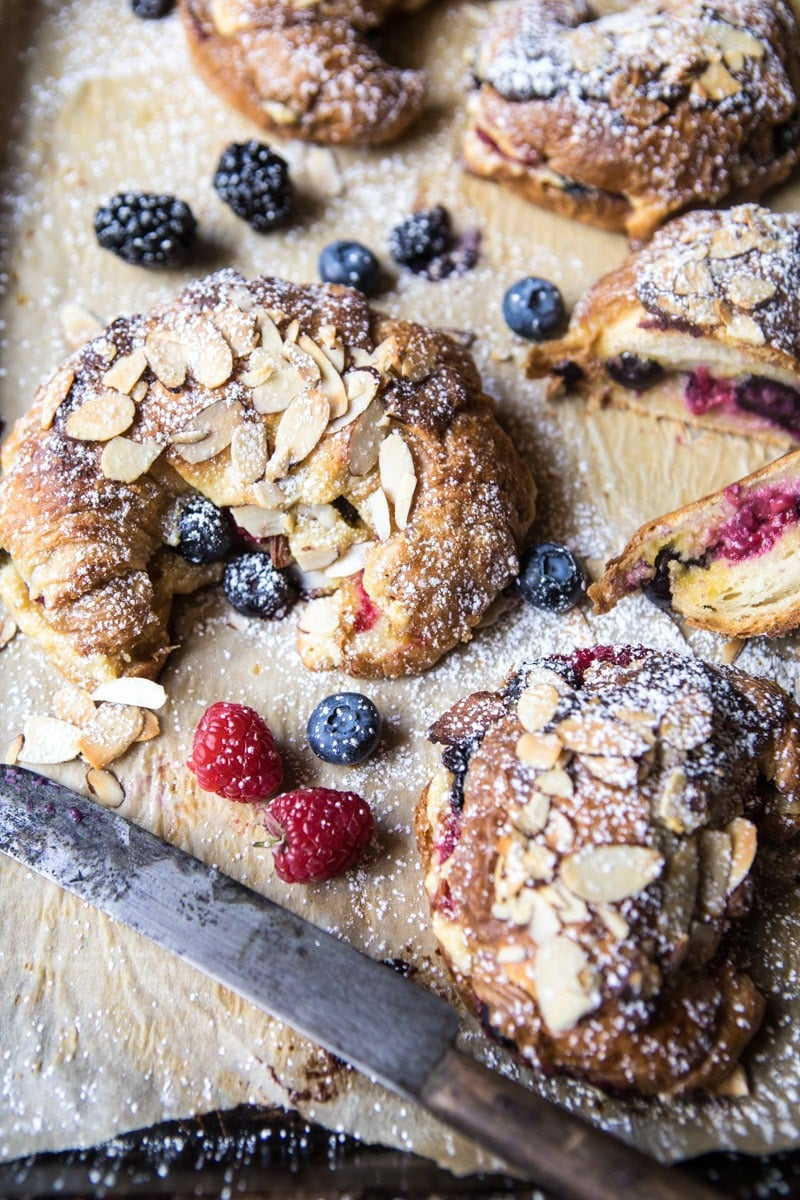
\includegraphics[width=1\textwidth,height=\textheight]{images/mixed-berry-almond-croissants.jpg}

\textbf{Prep Time:} 20 min \textbar{} \textbf{Cook Time:} 15 min
\textbar{} \textbf{Total Time:} 35 min

\section{Ingredients}\label{ingredients-77}

\begin{itemize}
\tightlist
\item
  2 tablespoons honey
\item
  1/4 cup bourbon ((optional))
\item
  2 pinches kosher salt
\item
  8 tablespoons unsalted butter, softened
\item
  2 eggs
\item
  1 teaspoon vanilla extract
\item
  1 1/4 cups almond meal ((finely ground almonds))
\item
  8 plain croissants, homemade or store-bought
\item
  2 cups mixed berries
\item
  1/4 cup flaked almonds
\end{itemize}

\section{Instructions}\label{instructions-77}

\begin{enumerate}
\def\labelenumi{\arabic{enumi}.}
\tightlist
\item
  Preheat the oven to 350 degrees F. Line a baking sheet with parchment
  paper.
\item
  In a small sauce pan, combine 1 cup water with the honey and bourbon,
  if using. Add a pinch of salt and bring to a boil over high heat. Once
  boiling remove from the heat and set aside.
\item
  In a medium bowl, beat together the butter, eggs, and vanilla until
  creamy. Add the almond meal and a pinch of salt and mix until
  combined.
\item
  Cut the croissants in half lengthwise and using a pastry brush, brush
  each piece lightly with the honey Bourbon mixture. Spread the bottom
  half the the croissant with almond cream and the top with enough
  berries to almost cover the surface of the croissant. Add the top half
  and place on the prepared baking sheet. Repeat with the remaining
  croissants, reserving 1/4 cup cream for topping. Spread the remaining
  cream over top of the croissants and top with flaked almonds. Transfer
  to the oven and bake for 12-15 minutes or until the croissants are
  golden. Remove from the oven and let sit on the pan for 5 minutes.
  Dust generously with powered sugar. Eat!
\end{enumerate}

\bookmarksetup{startatroot}

\chapter{Honey Thyme and Sweet Cherry Grilled
Brie}\label{honey-thyme-and-sweet-cherry-grilled-brie}

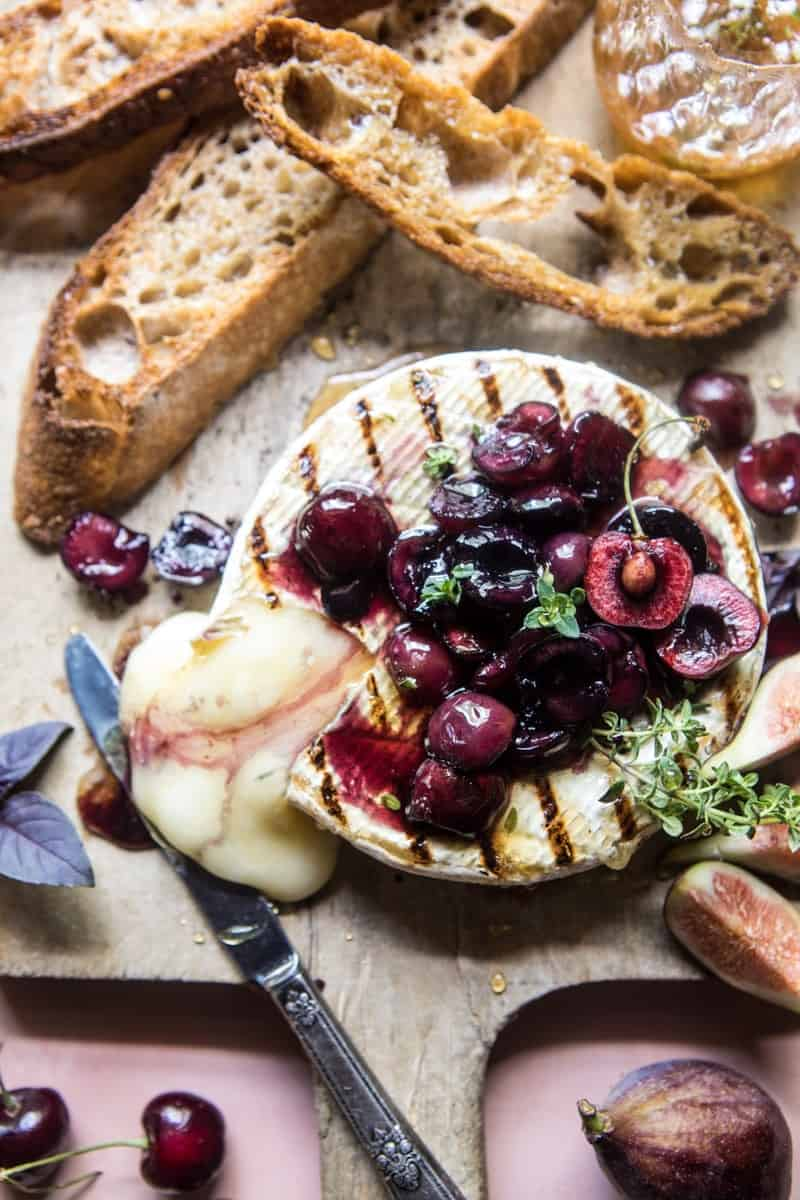
\includegraphics[width=1\textwidth,height=\textheight]{images/honey-thyme-and-sweet-cherry-grilled-brie.jpg}

\textbf{Prep Time:} 10 min \textbar{} \textbf{Cook Time:} 15 min
\textbar{} \textbf{Total Time:} 25 min

\section{Ingredients}\label{ingredients-78}

\begin{itemize}
\tightlist
\item
  1/3 cup honey
\item
  4 sprigs fresh thyme
\item
  pinch of flakey sea salt
\item
  1 (8 ounce) brie wheel
\item
  1 tablespoon butter or olive oil, plus more for rubbing
\item
  1 cup pitted cherries
\item
  1-2 tablespoons bourbon ((optional))
\item
  toasted or grilled bread, for serving
\end{itemize}

\section{Instructions}\label{instructions-78}

\begin{enumerate}
\def\labelenumi{\arabic{enumi}.}
\tightlist
\item
  Add the honey, thyme, and salt to a small saucepan and simmer over
  medium heat until it begins to boil. Remove from the heat let the
  honey sit 5 minutes or until ready to serve. You can make the honey up
  to a week in advance.
\item
  Preheat your grill or grill pan to high heat. Rub the brie with a
  little olive oil and sprinkle with salt. Place on the grill and grill
  for about 2-3 minutes per side or until the brie feels warm and gooey
  inside. Be careful when flipping the brie, you do not want to break
  the brie open. Carefully remove from the grill.
\item
  Meanwhile, add the butter, cherries, and bourbon (if using), to a
  small skillet set over medium high heat. Cook stirring occasionally
  until the cherries begin to release their juices, about 5 minutes.
  Remove from the heat.
\item
  To serve, place the warm brie on a serving plate. Top with cherries
  and drizzle generously with honey. Enjoy with toasted bread or
  crackers!
\end{enumerate}

\bookmarksetup{startatroot}

\chapter{My Favorite Buttermilk Pie
Crust}\label{my-favorite-buttermilk-pie-crust}

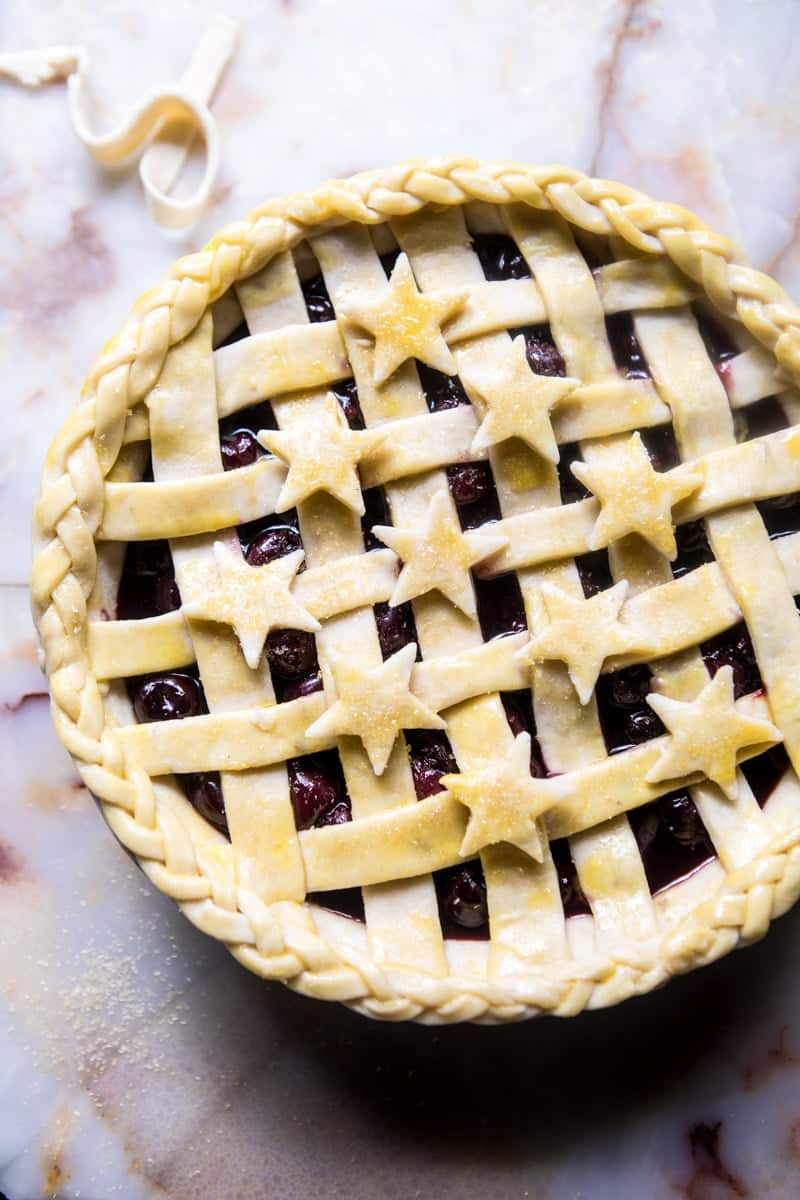
\includegraphics[width=1\textwidth,height=\textheight]{images/my-favorite-buttermilk-pie-crust.jpg}

\textbf{Prep Time:} 15 min \textbar{} \textbf{Cook Time:} \textbar{}
\textbf{Total Time:} 15 min

\section{Ingredients}\label{ingredients-79}

\begin{itemize}
\tightlist
\item
  2 1/2 cups all-purpose flour, plus more for rolling
\item
  1/3 cup almond flour
\item
  1 teaspoon kosher salt
\item
  1 cup chilled unsalted butter, cut into small cubes
\item
  1/3 cup cold buttermilk, plus more if needed
\end{itemize}

\section{Instructions}\label{instructions-79}

\begin{enumerate}
\def\labelenumi{\arabic{enumi}.}
\tightlist
\item
  Place the flour, almond flour, and salt in a large bowl. Add butter
  and use your fingers or a pastry cutter to work the butter into the
  flour until the mixture resembles small peas.
\item
  Pour in the buttermilk and mix with a spatula, drizzling in more
  buttermilk as needed (no more than 1 tablespoon at a time), until the
  dough just comes together (a few dry spots are ok). Turn the dough out
  onto a floured surface and gently knead until no dry spots remain,
  about 1 minute.
\item
  Divide the dough in half. Shape each piece into a circular disk. Wrap
  the dough in plastic wrap. At this point you can place the dough in
  the fridge for up to one week or use as directed in your recipe.
\end{enumerate}

\bookmarksetup{startatroot}

\chapter{Jalapeño Cheddar Guacamole Turkey Burgers with Crispy
Onions}\label{jalapeuxf1o-cheddar-guacamole-turkey-burgers-with-crispy-onions}

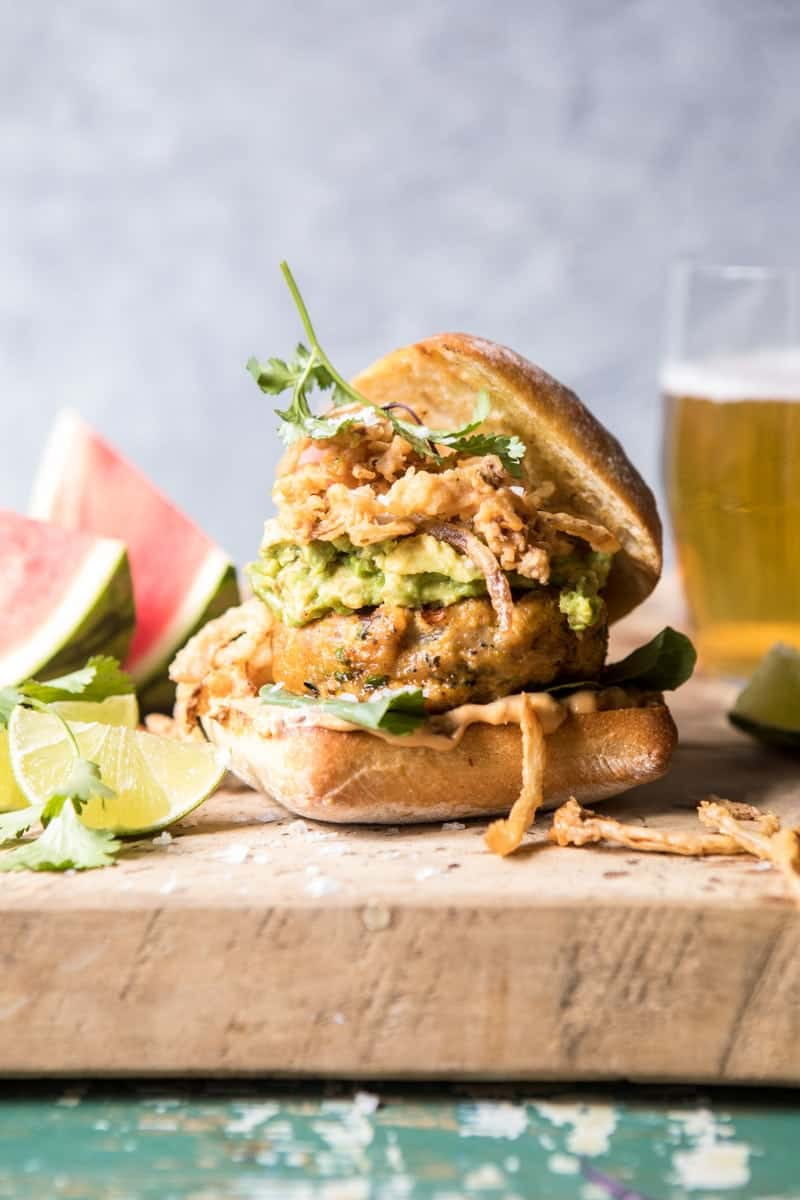
\includegraphics[width=1\textwidth,height=\textheight]{images/jalape-o-cheddar-guacamole-turkey-burgers-with-crispy-onions.jpg}

\textbf{Prep Time:} 25 min \textbar{} \textbf{Cook Time:} 25 min
\textbar{} \textbf{Total Time:} 50 min

\section{Ingredients}\label{ingredients-80}

\begin{itemize}
\tightlist
\item
  2 jalapeños
\item
  1 pound ground turkey or chicken
\item
  1/2 cup grated cheddar cheese
\item
  1/3 cup panko bread crumbs
\item
  1 egg
\item
  1 teaspoon smoked paprika
\item
  kosher salt and pepper
\item
  4 slices smoked gouda or cheddar
\item
  4 burger buns, toasted
\item
  2 avocados lightly mashed
\item
  juice from 1 lime
\item
  chipotle mayo and fresh cilantro, for serving
\item
  2 large white onions, halved and then sliced very thin
\item
  2 cups buttermilk
\item
  2 cups flour
\item
  Kosher salt and pepper
\item
  oil, for frying
\end{itemize}

\section{Instructions}\label{instructions-80}

\begin{enumerate}
\def\labelenumi{\arabic{enumi}.}
\tightlist
\item
  Preheat the broiler to high. Place the jalapeños on a baking sheet
  and place under the broiler. Broil until charred all over, about 5
  minutes. Remove and let cool and then seed and chop the jalapeños.
\item
  In a medium bowl, combine the jalapeños, turkey, cheddar, panko, egg,
  paprika, salt, and pepper. Mix until just combined and then shape the
  mix into 4 even size burger patties.
\item
  Preheat the outdoor grill or grill pan to high. Grill the burger for 5
  minute per side or until cooked through. During the last minute of
  cooking add the cheese slices.
\item
  To assemble, spread the chipotle mayo on the bottom of each bun. Top
  with a burger, avocado, lime juice and a pinch of salt. Add the crispy
  onions (recipe follows) and cilantro. EAT
\end{enumerate}

\bookmarksetup{startatroot}

\chapter{Lemon Feta Dip with Garlic Tomato
Vinaigrette}\label{lemon-feta-dip-with-garlic-tomato-vinaigrette}

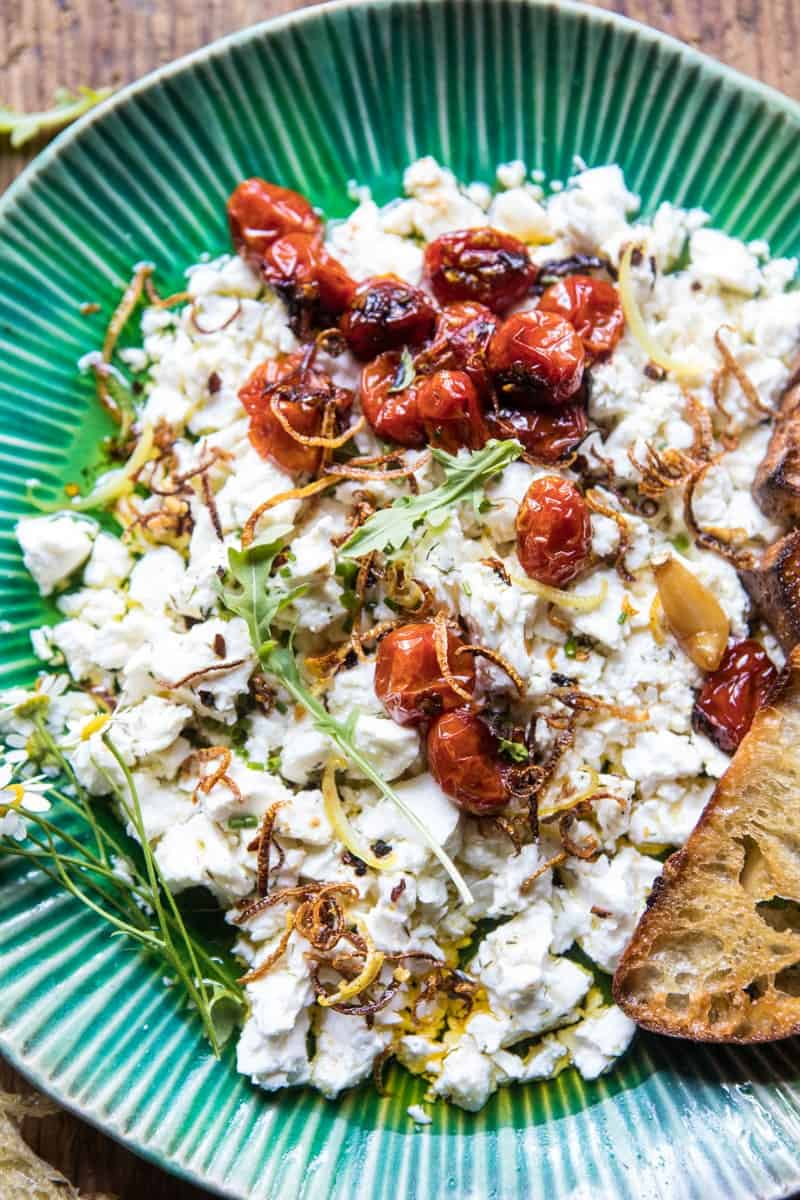
\includegraphics[width=1\textwidth,height=\textheight]{images/lemon-feta-dip-with-garlic-tomato-vinaigrette.jpg}

\textbf{Prep Time:} 5 min \textbar{} \textbf{Cook Time:} 15 min
\textbar{} \textbf{Total Time:} 20 min

\section{Ingredients}\label{ingredients-81}

\begin{itemize}
\tightlist
\item
  1/3 cup extra virgin olive oil
\item
  1 1/2 cups small cherry tomatoes
\item
  3 cloves garlic, smashed
\item
  1 teaspoon crushed red pepper flakes, or to taste
\item
  the rind from 1 lemon, thinly sliced
\item
  1 tablespoon fresh oregano leaves
\item
  pinch of flaky sea salt and pepper
\item
  8 ounces feta cheese, finely crumbled
\item
  1 tablespoon fresh dill, roughly chopped
\item
  1 tablespoon fresh chives, chopped
\item
  fresh arugula for serving
\item
  toast, bread or pita for serving
\end{itemize}

\section{Instructions}\label{instructions-81}

\begin{enumerate}
\def\labelenumi{\arabic{enumi}.}
\tightlist
\item
  Heat a medium skillet over medium heat. Add the olive oil, tomatoes,
  garlic, crushed red pepper flakes, oregano, lemon rind and a pinch
  each of salt and pepper. Cook until the tomatoes just begin to burst
  and the garlic is fragrant, about 10-15 minutes. Remove from the heat
  and let cool slightly.
\item
  Crumble the feta into a serving bowl. Drizzle the tomatoes and oil
  over the feta. Top with fresh dill, chives, and arugula. Serve with
  bread or pita for scooping. Enjoy!
\end{enumerate}

\bookmarksetup{startatroot}

\chapter{Grilled Thai Satay Chicken}\label{grilled-thai-satay-chicken}

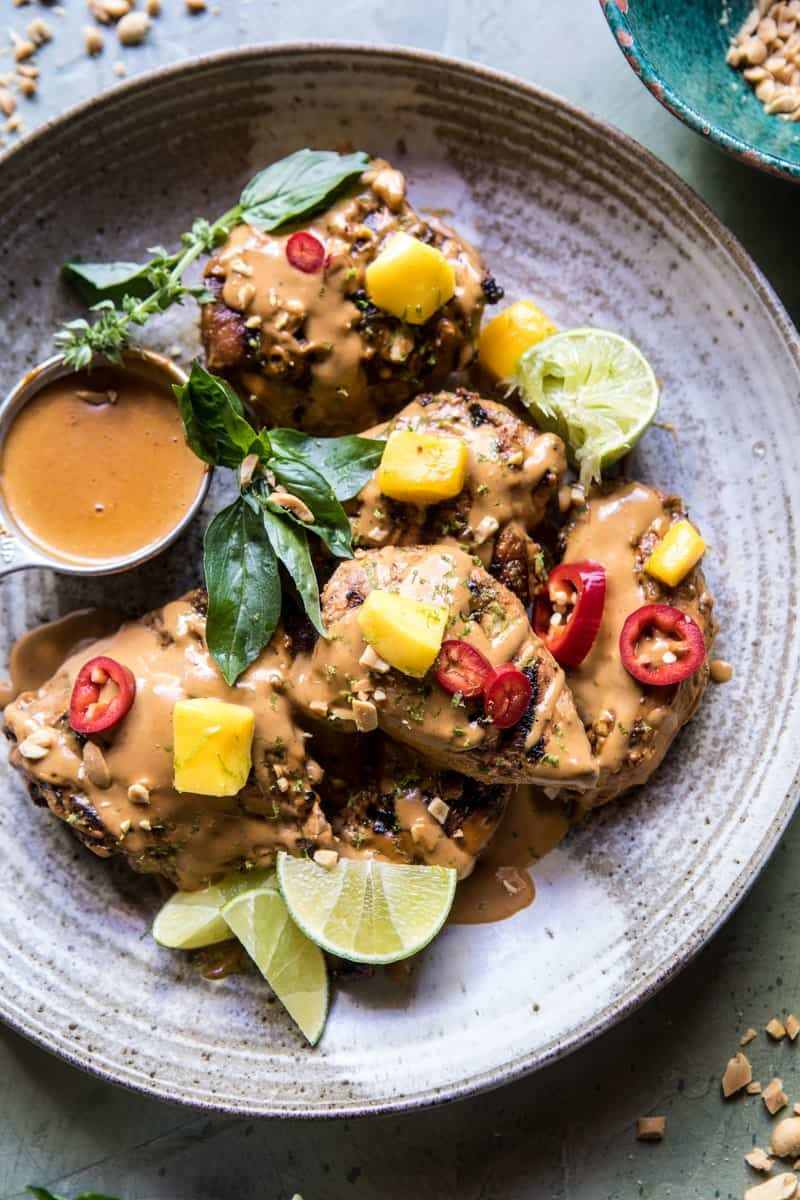
\includegraphics[width=1\textwidth,height=\textheight]{images/grilled-thai-satay-chicken.jpg}

\textbf{Prep Time:} 15 min \textbar{} \textbf{Cook Time:} 15 min
\textbar{} \textbf{Total Time:} 1 hr

\section{Ingredients}\label{ingredients-82}

\begin{itemize}
\tightlist
\item
  2 pounds boneless chicken breast or small thighs ((I used a mix of
  breast and thighs))
\item
  1/2 cup canned unsweetened coconut milk
\item
  1/4 cup low sodium soy sauce
\item
  1/4 cup honey
\item
  2 tablespoons Thai red curry paste
\item
  quinoa or rice, for serving
\item
  fresh cilantro or thai basil, for serving
\item
  limes, mango, peanuts and chili peppers for serving
\item
  1 (14 ounce) can unsweetened coconut milk
\item
  1/2 cup creamy peanut butter
\item
  2 tablespoons fish sauce
\item
  2 tablespoons low sodium soy sauce
\item
  2 tablespoons Thai red curry paste
\item
  2 teaspoons tamarind ((optional))
\item
  juice of lime
\end{itemize}

\section{Instructions}\label{instructions-82}

\begin{enumerate}
\def\labelenumi{\arabic{enumi}.}
\tightlist
\item
  Whisk together the coconut milk, soy sauce, Thai red curry paste, and
  honey, in a small bowl. Remove 1/4 cup of the marinade and reserve for
  cooking. Add the chicken to a large ziplock bag and pour the remaining
  marinade over the chicken. Let sit for 30 minutes or up to overnight
  in the fridge.
\item
  Meanwhile, make the peanut sauce. In a small sauce pan, combine all
  the ingredients and set over medium low heat, cook stirring often
  until the sauce is smooth and drizzle-able. Stir in the lime juice. If
  the sauce seem thick, add water to thin. Keep sauce warm.
\item
  Preheat an outdoor grill or grill pan to medium heat. Oil the grates.
\item
  Add the chicken and grill for 5-8 minutes per side, brushing the
  chicken with the reserved coconut milk mixture until the chicken is
  cooked through. Remove from the grill and arrange on a serving plate.
  Drizzle the peanut sauce over the chicken.
\item
  Serve the chicken over top of a bed of quinoa or rice with fresh
  mango, limes, and cilantro. Enjoy!
\end{enumerate}

\bookmarksetup{startatroot}

\chapter{Roasted Summer Berry Piñata Ice Cream
Cake}\label{roasted-summer-berry-piuxe3ata-ice-cream-cake}

\textbf{Prep Time:} 1 hr \textbar{} \textbf{Cook Time:} 50 min
\textbar{} \textbf{Total Time:} 1 hr 50 min

\section{Ingredients}\label{ingredients-83}

\begin{itemize}
\tightlist
\item
  3 cups vanilla ice cream, softened
\item
  2 1/2 cups all-purpose flour
\item
  2 teaspoons baking powder
\item
  1 teaspoon kosher salt
\item
  2 sticks unsalted butter, at room temperature
\item
  1 1/4 cups granulated sugar
\item
  3 whole eggs
\item
  1 cup buttermilk
\item
  2 teaspoons vanilla extract
\item
  3 cups mixed berries, plus fresh berries for serving
\item
  2 tablespoons honey
\item
  3 sticks salted butter, at room temperature
\item
  1 1/2 cups powdered sugar
\item
  1/2 cup heavy whipping cream
\item
  2 teaspoons vanilla extract
\end{itemize}

\section{Instructions}\label{instructions-83}

\begin{enumerate}
\def\labelenumi{\arabic{enumi}.}
\tightlist
\item
  Line one (8 inch) spring form pan with plastic wrap. Spread the ice
  cream in one even layer. Freeze until firm, 6 hours or overnight. Once
  Frozen, cut a 10cm round from the center of the cake. Remove center
  and save for later. Place the ice cream back in the freezer.
\item
  To make the cake. Preheat the oven to 350 degrees F. Line 2 (8-inch)
  round cake pans with parchment paper, then grease with butter.
\item
  In a medium size bowl combine the flour, baking powder and salt. In
  the bowl of a stand mixer (or use a hand-held mixer) beat together the
  butter and sugar until light and fluffy. With the mixer on low, beat
  in the eggs. Add the vanilla and beat until combined. Slowly add the
  dry ingredients to the wet ingredients with the mixer on low,
  alternating with the buttermilk and ending with flour until just
  combined.
\item
  Pour the batter among the cake pans and bake 25-30 minutes, until the
  tops are just set and no longer wiggly in the center. Remove and let
  cool five minutes, then turn the cakes out onto a rack to cool
  further. To one of the cakes, cut a 10cm round from the center. Remove
  the center and discard. Keep the remaining cake layer whole. Freeze
  the cakes until frozen, at least 2 hours.
\item
  To make the berries. Preheat the oven to 400 degrees F. In a 9x13 inch
  baking dish, combine the berries and honey. Transfer to the oven and
  roast for 15-20 minutes or until the berries have burst and released
  their juice. Let cool.
\item
  To make the buttercream. Add the butter and powdered sugar to the bowl
  of a stand mixer. Beat the butter and powdered sugar together until
  the butter is light and fluffy. Add the vanilla and continue beating,
  scraping down the sides as needed, for another 2 minutes. Add the
  heavy cream and whip the frosting for 2-4 minutes more or until light
  and fluffy.
\item
  To assemble the cake. Lay the vanilla cake layer, the one with the
  hole cut out of the center, flat on a serving plate. Spread with
  buttercream over the cake, then add half roasted berries over the
  buttercream. Add the ice cream cake layer and again, spread the
  buttercream over the ice cream and inside the hole. Spread the
  remaining roasted berries on top of the buttercream ice cream layer.
  Freeze 2 hours or until firm.
\item
  Remove the cake from the freezer and fill the hole with fresh berries.
  Now add the remaining vanilla cake layer and frost the cake all over
  with the remaining buttercream. Freeze another 2 hours or until firm.
  Just before serving, decorate the top of the cake with berries. Slice
  and enjoy!
\end{enumerate}

\bookmarksetup{startatroot}

\chapter{Blueberry, Melon, Feta, Fruit Salad
Stacks}\label{blueberry-melon-feta-fruit-salad-stacks}

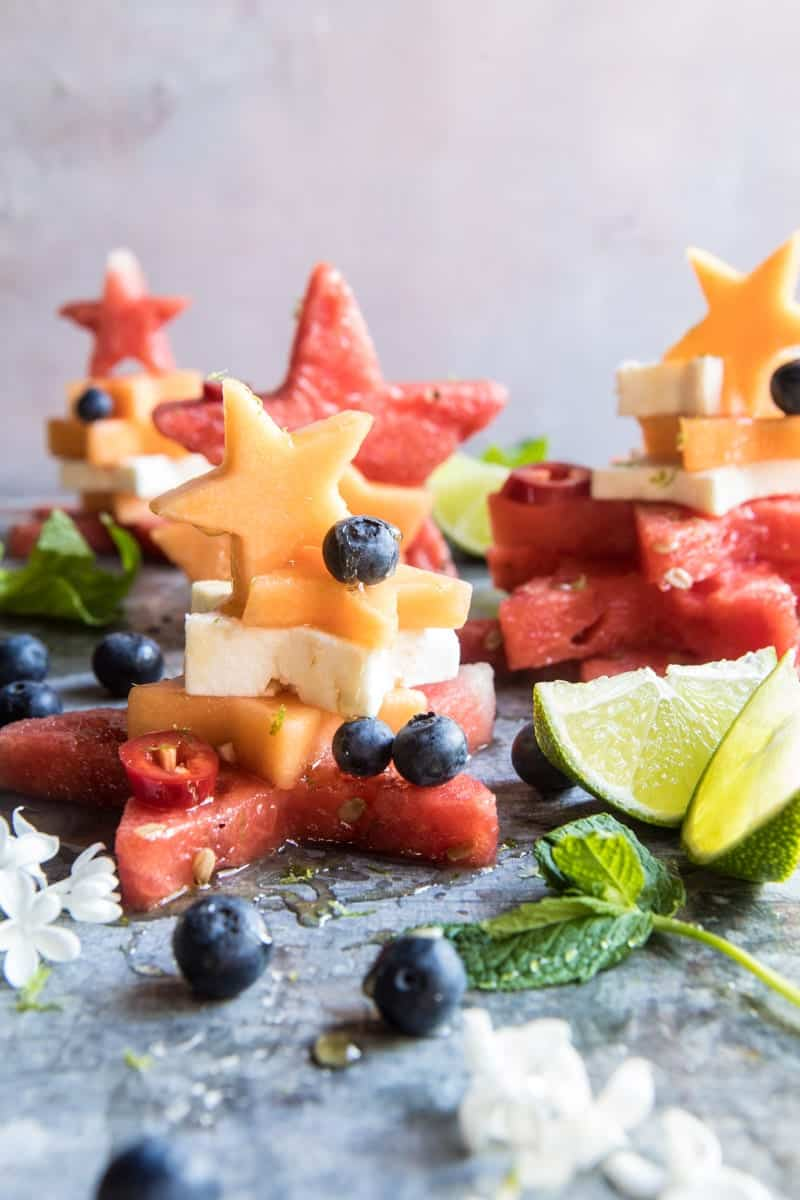
\includegraphics[width=1\textwidth,height=\textheight]{images/blueberry-melon-feta-fruit-salad-stacks.jpg}

\textbf{Prep Time:} 15 min \textbar{} \textbf{Cook Time:} \textbar{}
\textbf{Total Time:} 15 min

\section{Ingredients}\label{ingredients-84}

\begin{itemize}
\tightlist
\item
  1 small seedless watermelon
\item
  1 small cantaloupe
\item
  1 cup blueberries
\item
  juice and zest from 2 limes
\item
  1 tablespoon honey plus, more to taste
\item
  1 fresno chile pepper, thinly sliced (optional)
\item
  fresh mint and or basil
\item
  flaky sea salt
\item
  1 (8 ounce) block feta cheese, sliced into 1/4 inch slices or crumbled
\end{itemize}

\section{Instructions}\label{instructions-84}

\begin{enumerate}
\def\labelenumi{\arabic{enumi}.}
\tightlist
\item
  Slice the watermelon and cantaloupe into 1/2 inch slices. Remove the
  seeds from the cantaloupe. Cut the fruit slices into stars using
  cookie cutters or cut into 1 inch cubes. Do the same with the feta.
  Arrange the fruit and on a large serving plate or layer into stacks.
  Save the scraps for snaking on.
\item
  Sprinkle the blueberries over top.
\item
  In a small bowl, stir together the zest of 1 lime and the juice of 2
  limes, the honey, and the fresno pepper. Drizzle the dressing over the
  fruit. Add the fresh mint and a sprinkle of salt. Serve the fruit
  chilled, with extra honey if desired.
\end{enumerate}

\bookmarksetup{startatroot}

\chapter{Farmer Market Pickled Crudité
Platter}\label{farmer-market-pickled-crudituxe3-platter}

\textbf{Prep Time:} 15 min \textbar{} \textbf{Cook Time:} \textbar{}
\textbf{Total Time:} 15 min

\section{Ingredients}\label{ingredients-85}

\begin{itemize}
\tightlist
\item
  1-2 cups hummus, homemade or store-bought
\item
  olive oil, for drizzling
\item
  2 cups whole milk ricotta cheese
\item
  1 cup basil pesto, homemade or store-bought
\item
  4 cups assorted pickled veggies
\item
  2 cups fresh sliced veggies and or fruits
\end{itemize}

\section{Instructions}\label{instructions-85}

\begin{enumerate}
\def\labelenumi{\arabic{enumi}.}
\tightlist
\item
  Spread the hummus on a large serving board or platter, or serve it in
  a bowl. Drizzle with olive oil and sprinkle with spices, if desired.
\item
  Add the ricotta to a bowl and swirl with the pesto.
\item
  Arrange both the pickled veggies and fresh fruits around the dips.
  Serve.
\end{enumerate}

\bookmarksetup{startatroot}

\chapter{Quick Pickled Veggies}\label{quick-pickled-veggies}

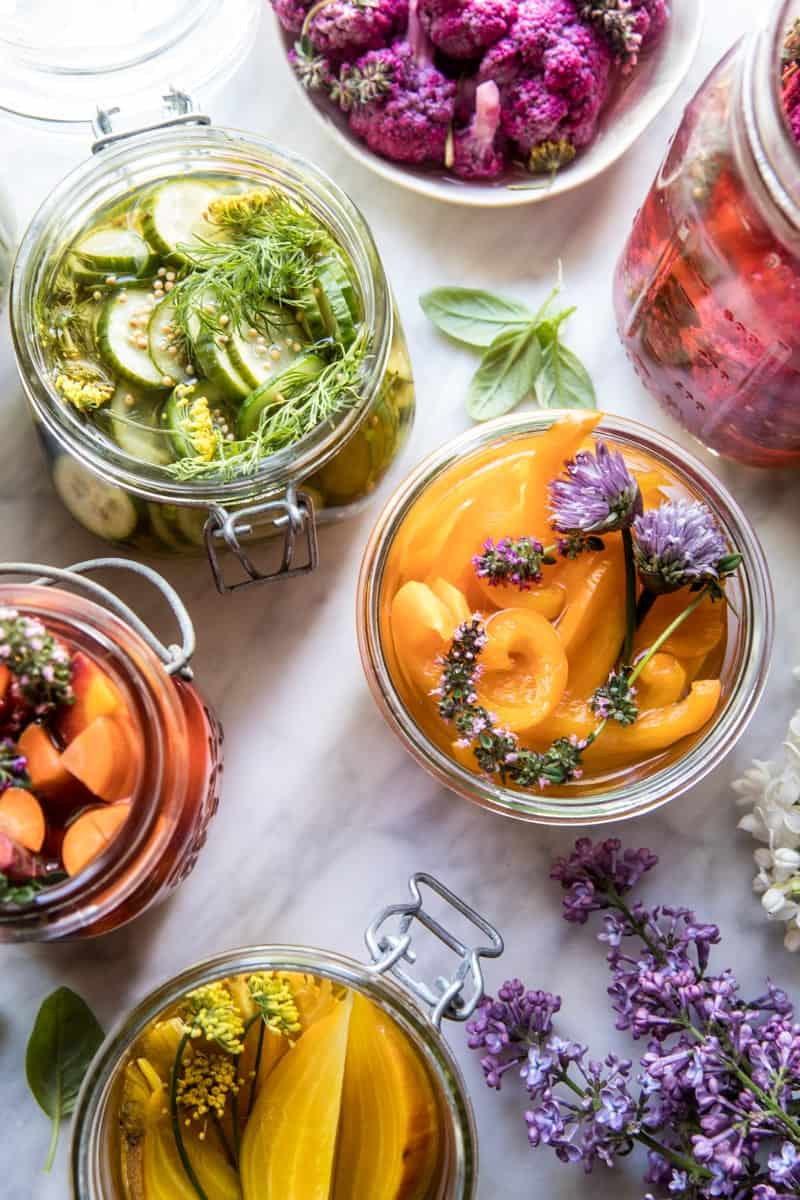
\includegraphics[width=1\textwidth,height=\textheight]{images/quick-pickled-veggies.jpg}

\textbf{Prep Time:} 15 min \textbar{} \textbf{Cook Time:} 5 min
\textbar{} \textbf{Total Time:} 20 min

\section{Ingredients}\label{ingredients-86}

\begin{itemize}
\tightlist
\item
  fresh herbs, such as thyme, rosemary, basil, and dill
\item
  2-4 cloves garlic, smashed
\item
  1 teaspoon each black peppers and coriander seeds
\item
  crush red pepper flakes or sliced chile peppers (optional)
\item
  2 pounds fresh fruits and veggies such as carrots, beets, cauliflower,
  asparagus, cherries, and strawberries
\item
  2 cups apple cider vinegar
\item
  2 cups water
\item
  1/4 cup kosher salt
\item
  2 tablespoons honey or sugar
\item
  zest and juice of 1 lemon
\end{itemize}

\section{Instructions}\label{instructions-86}

\begin{enumerate}
\def\labelenumi{\arabic{enumi}.}
\tightlist
\item
  If using, divide the herbs - garlic, peppercorns, coriander seeds, and
  chile flakes, among glass jars. Pack the fruits and veggies into the
  jars, packing them in tight, but leaving a 1/2 inch space at the top
  of the jar.
\item
  In a large pot, bring the vinegar, water, salt, and honey to a boil
  over high heat, stirring until the salt has dissolved. Remove from the
  heat and stir in the lemon zest and juice. Pour the pickling brine
  over the fruits and veggies, filling the jars up to 1/2 inch from the
  top. Seal the jars and let them cool at room temperature. Chill at
  least 4 hours and up to 2 months. The longer the fruits and veggies
  sit, the more flavor they will develop.
\end{enumerate}

\bookmarksetup{startatroot}

\chapter{Blackberry Lilac Mojito}\label{blackberry-lilac-mojito}

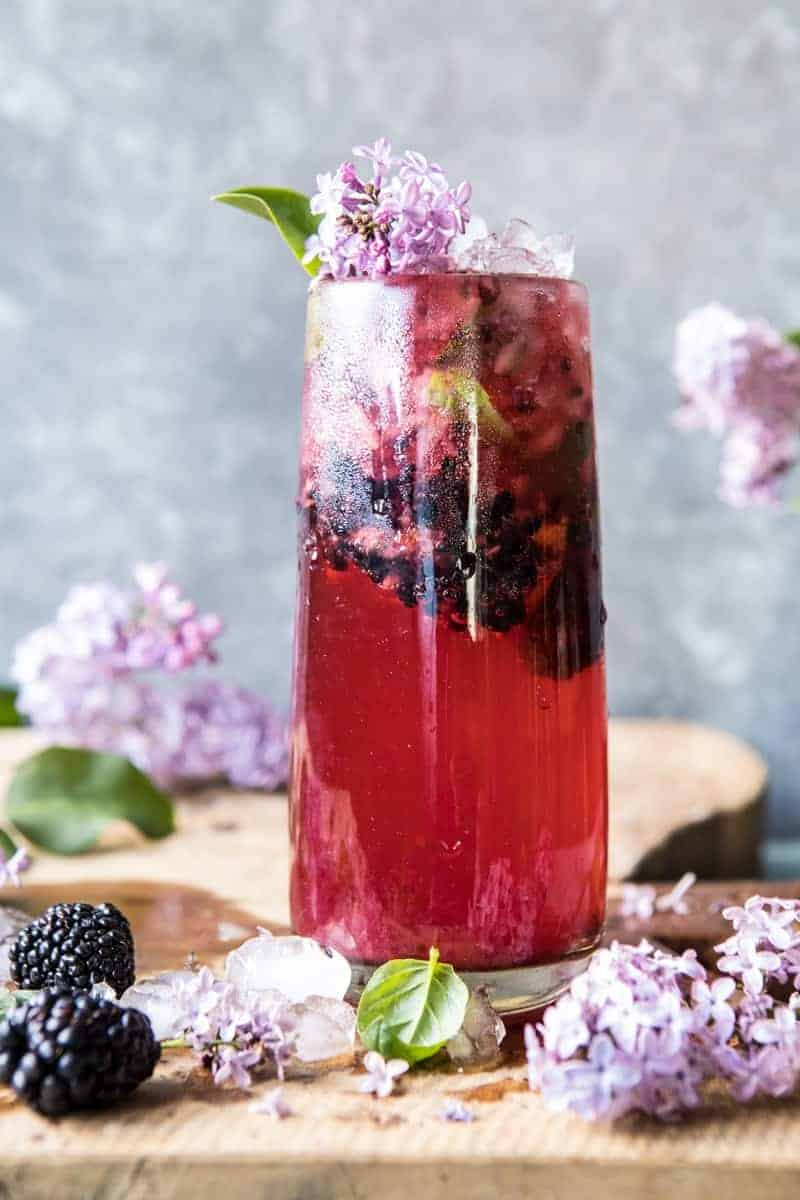
\includegraphics[width=1\textwidth,height=\textheight]{images/blackberry-lilac-mojito.jpg}

\textbf{Prep Time:} 10 min \textbar{} \textbf{Cook Time:} 10 min
\textbar{} \textbf{Total Time:} 20 min

\section{Ingredients}\label{ingredients-87}

\begin{itemize}
\tightlist
\item
  1/2 lemon, cut into wedges
\item
  6-8 fresh blackberries
\item
  8-12 leaves fresh basil
\item
  1-2 tablespoons lilac syrup or 1-2 teaspoons sweetener of choice
\item
  2 ounces rum
\item
  sparkling water, for topping
\item
  3/4 cup water
\item
  1/3 cup honey
\item
  1/2 cup fresh lilac flowers or 1-2 tablespoons dried lavender
\end{itemize}

\section{Instructions}\label{instructions-87}

\begin{enumerate}
\def\labelenumi{\arabic{enumi}.}
\tightlist
\item
\end{enumerate}

\bookmarksetup{startatroot}

\chapter{Farmers Market Goat Cheese Pasta Primavera with Marinated
Veggies}\label{farmers-market-goat-cheese-pasta-primavera-with-marinated-veggies}

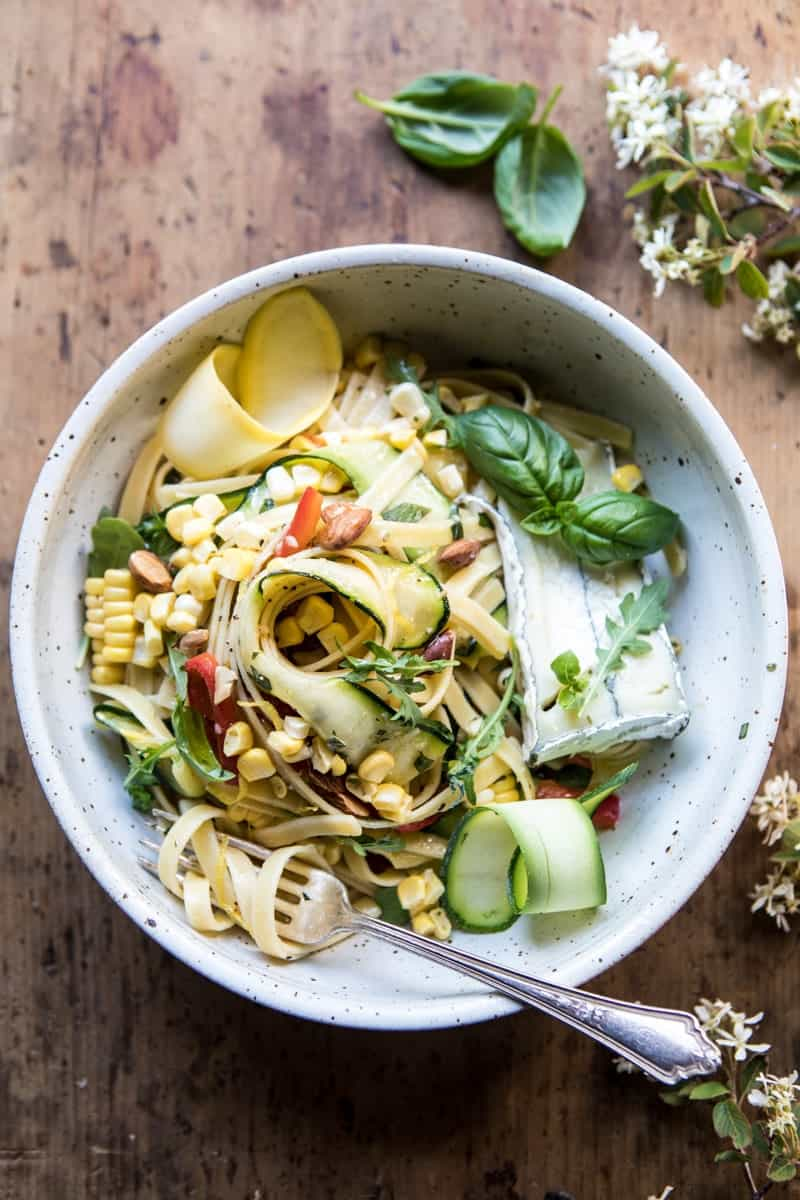
\includegraphics[width=1\textwidth,height=\textheight]{images/farmers-market-goat-cheese-pasta-primavera-with-marinated-veggies.jpg}

\textbf{Prep Time:} 15 min \textbar{} \textbf{Cook Time:} 10 min
\textbar{} \textbf{Total Time:} 25 min

\section{Ingredients}\label{ingredients-88}

\begin{itemize}
\tightlist
\item
  1/3 cup extra virgin olive oil
\item
  2 tablespoons balsamic vinegar
\item
  1 clove garlic, minced or grated
\item
  juice + zest of 1 lemon
\item
  1/4 cup fresh basil, chopped
\item
  1 tablespoon chopped fresh oregano
\item
  pinch of crushed red pepper flakes
\item
  kosher salt and pepper
\item
  1 small zucchini, cut into ribbons
\item
  1 small yellow squash, cut into ribbons
\item
  1 red bell pepper, sliced thin
\item
  2 ears corn, kernels removed from the cob
\item
  1 (12 ounce) jar marinated artichokes, drained
\item
  1 pound fettuccine pasta
\item
  1/2 cup grated parmesan cheese
\item
  6 ounces aged or creamy goat cheese, crumbled
\item
  fresh arugula and toasted almonds, for serving
\end{itemize}

\section{Instructions}\label{instructions-88}

\begin{enumerate}
\def\labelenumi{\arabic{enumi}.}
\tightlist
\item
  In a medium bowl, combine the olive oil, balsamic vinegar, garlic,
  lemon zest and juice, basil, oregano, crushed red pepper flakes, and a
  pinch each of salt and pepper. Add the zucchini, yellow squash, red
  pepper, corn, and artichokes and toss to combine.
\item
  Bring a large pot of salted water to a boil. Cook the pasta according
  to package directions until al dente. Just before draining, remove 1
  cup of the pasta cooking water. Drain and add the pasta right back to
  the pot. Add the 1/4 cup pasta cooking water, the parmesan, veggies
  and any oil left in the bowl and toss well to combine.
\item
  Divide the pasta among bowls and top with goat cheese, arugula, and
  almonds. Eat!
\end{enumerate}

\bookmarksetup{startatroot}

\chapter{Honey Strawberry Apricot
Tart}\label{honey-strawberry-apricot-tart}

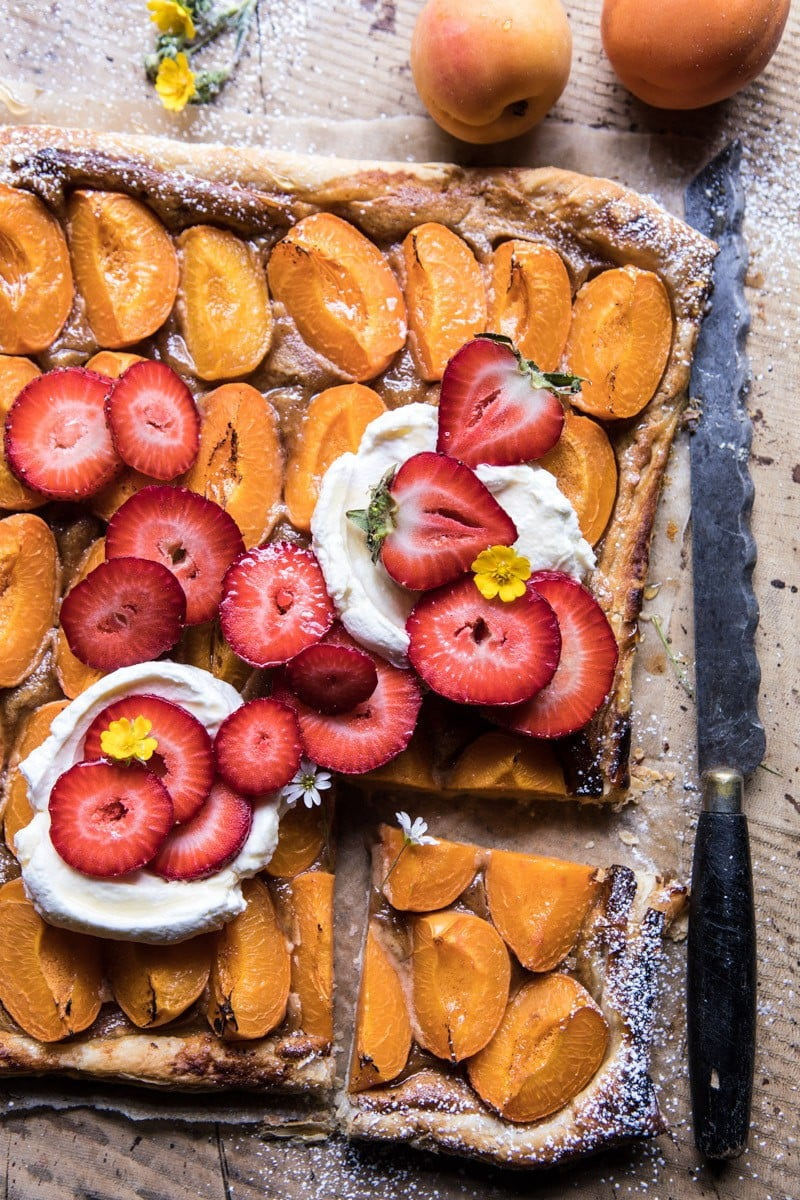
\includegraphics[width=1\textwidth,height=\textheight]{images/honey-strawberry-apricot-tart.jpg}

\textbf{Prep Time:} 15 min \textbar{} \textbf{Cook Time:} 30 min
\textbar{} \textbf{Total Time:} 45 min

\section{Ingredients}\label{ingredients-89}

\begin{itemize}
\tightlist
\item
  1/2 cup almonds, toasted
\item
  1/4 cup honey + more for drizzling
\item
  4 tablespoons butter, at room temperature + melted butter for crust
\item
  1 egg
\item
  1 teaspoon vanilla extract
\item
  1 sheet frozen puff pasty, thawed
\item
  12 apricots, quartered
\item
  4 ounces mascarpone cheese
\item
  1/2 cup heavy whipping cream
\item
  1 cup fresh strawberries, sliced
\item
  basil and powdered sugar, for serving
\end{itemize}

\section{Instructions}\label{instructions-89}

\begin{enumerate}
\def\labelenumi{\arabic{enumi}.}
\tightlist
\item
  Preheat the oven to 375 degrees F.
\item
  Pulse the almonds in a food processor until very finely ground. Add
  the honey, butter, egg, and vanilla and pulse until smooth.
\item
  On a lightly floured surface, roll the puff pastry out into a
  rectangle about 1/4 inch thick. Place the pastry on a parchment lined
  baking sheet and spread the almond cream over the pastry, leaving a
  1/4 inch border. Arrange the apricots over the cream and then drizzle
  with honey. Brush the edges of the pastry with melted butter. Transfer
  to the oven and bake for 25-30 minutes or until golden brown. It is OK
  if the edges get dark.
\item
  Meanwhile, whip the mascarpone and cream together until stiff peaks
  form.
\item
  Allow the tart to cool slightly and then serve dolloped with whipped
  cream and topped with fresh strawberries and a dusting of powdered
  sugar, if desired.
\end{enumerate}

\bookmarksetup{startatroot}

\chapter{Greek Roasted Cauliflower Burgers with Pan Fried Feta and
Tomato Olive
Salad}\label{greek-roasted-cauliflower-burgers-with-pan-fried-feta-and-tomato-olive-salad}

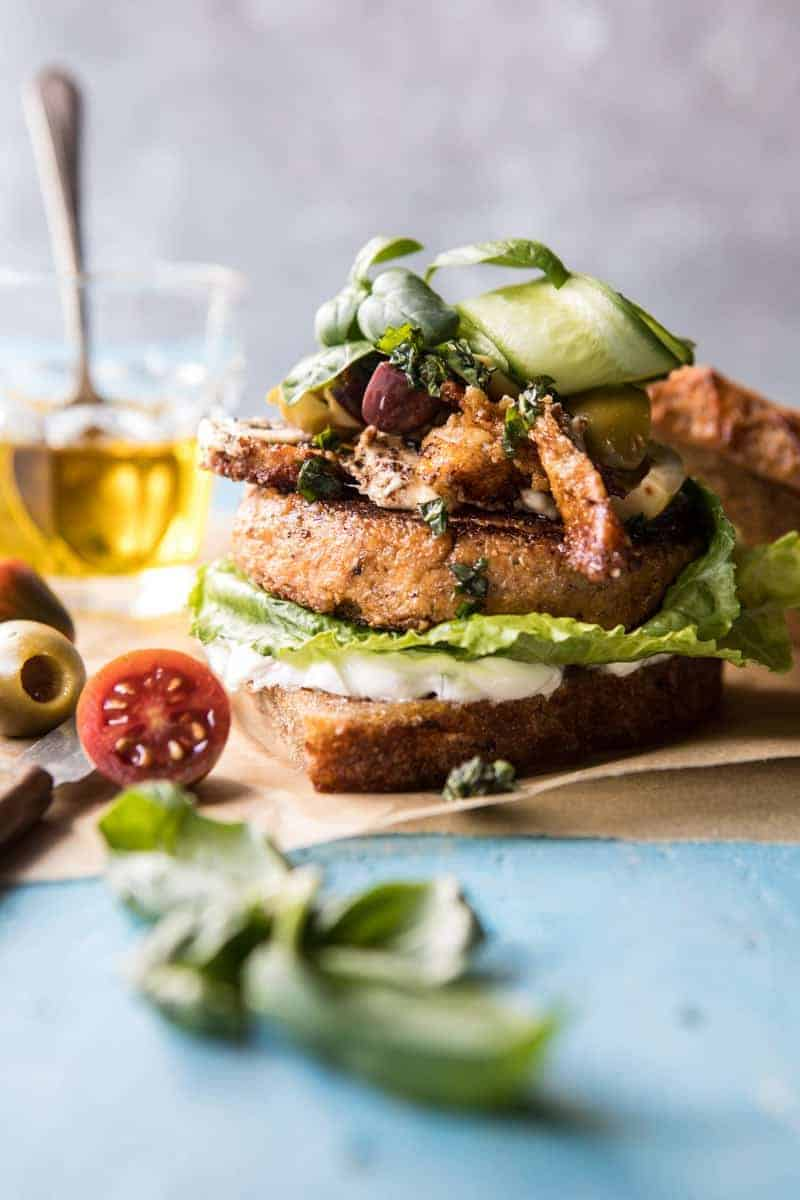
\includegraphics[width=1\textwidth,height=\textheight]{images/greek-roasted-cauliflower-burgers-with-pan-fried-feta-and-tomato-olive-salad.jpg}

\textbf{Prep Time:} 15 min \textbar{} \textbf{Cook Time:} 30 min
\textbar{} \textbf{Total Time:} 45 min

\section{Ingredients}\label{ingredients-90}

\begin{itemize}
\tightlist
\item
  1 medium head cauliflower, cut into florets
\item
  2 cloves garlic
\item
  2 tablespoons extra virgin olive oil
\item
  1 tablespoon chopped fresh oregano
\item
  1 tablespoon smoked paprika
\item
  kosher salt and pepper
\item
  1/2 cup raw walnuts
\item
  1 egg
\item
  1 cup cooked quinoa
\item
  6 ounces feta cheese, sliced into 1/4 inch slices
\item
  6 pieces whole grain bread, toasted
\item
  Tzatziki or yogurt, lettuce, and cucumber, for serving
\item
  1/2 cup cherry tomatoes halved
\item
  1/2 cup mixed olives pitted and halved
\item
  2 tablespoons extra virgin olive oil
\item
  1/4 cup fresh basil chopped
\item
  pinch of crushed red pepper flakes
\end{itemize}

\section{Instructions}\label{instructions-90}

\begin{enumerate}
\def\labelenumi{\arabic{enumi}.}
\tightlist
\item
  Preheat the oven to 400 degrees F. Line a baking sheet with parchment.
\item
  On a baking sheet, toss together the cauliflower, 2 tablespoons olive
  oil, oregano, paprika, salt and pepper. Transfer to the oven and roast
  for 15 minutes. Add the walnuts, toss, and return to the oven for
  another 10-15 minutes. Remove and let cool.
\item
  Add the cauliflower and walnuts to a food processor with the egg and
  quinoa. Pulse until combined. Pat the mixture into 6 even patties. The
  mixture will be sticky. If time allows, place in the fridge to chill,
  at least one hour or in the freezer for 15 minutes to make them easier
  to handle.
\item
  Meanwhile, make the salsa. In a medium bowl, combine the tomatoes,
  olives, 2 tablespoons olive oil, basil, crushed red pepper flakes, and
  a pinch of salt.
\item
  Heat a large skillet over medium-high heat. Add about a drizzle of
  olive oil. When the oil shimmers, add 2-3 patties at a time and cook
  until lightly browned, about 5-8 minutes, flip and cook another 5-8
  minutes or until firm. Repeat with the remaining patties. Note: these
  burgers are delicate, be careful when flipping.
\item
  In the same skillet, add another drizzle of olive oil. Add the feta
  slices and cook until golden brown, about 2 minutes, flip and cook
  until browned, about 1 minute.
\item
  To serve, spread each piece of bread with Tzatziki. Add the burger,
  fried feta, salsa, and cucumber. Add the top piece of bread. EAT.
\end{enumerate}

\bookmarksetup{startatroot}

\chapter{Mexican Grilled Corn with Green Chile Honey
Butter}\label{mexican-grilled-corn-with-green-chile-honey-butter}

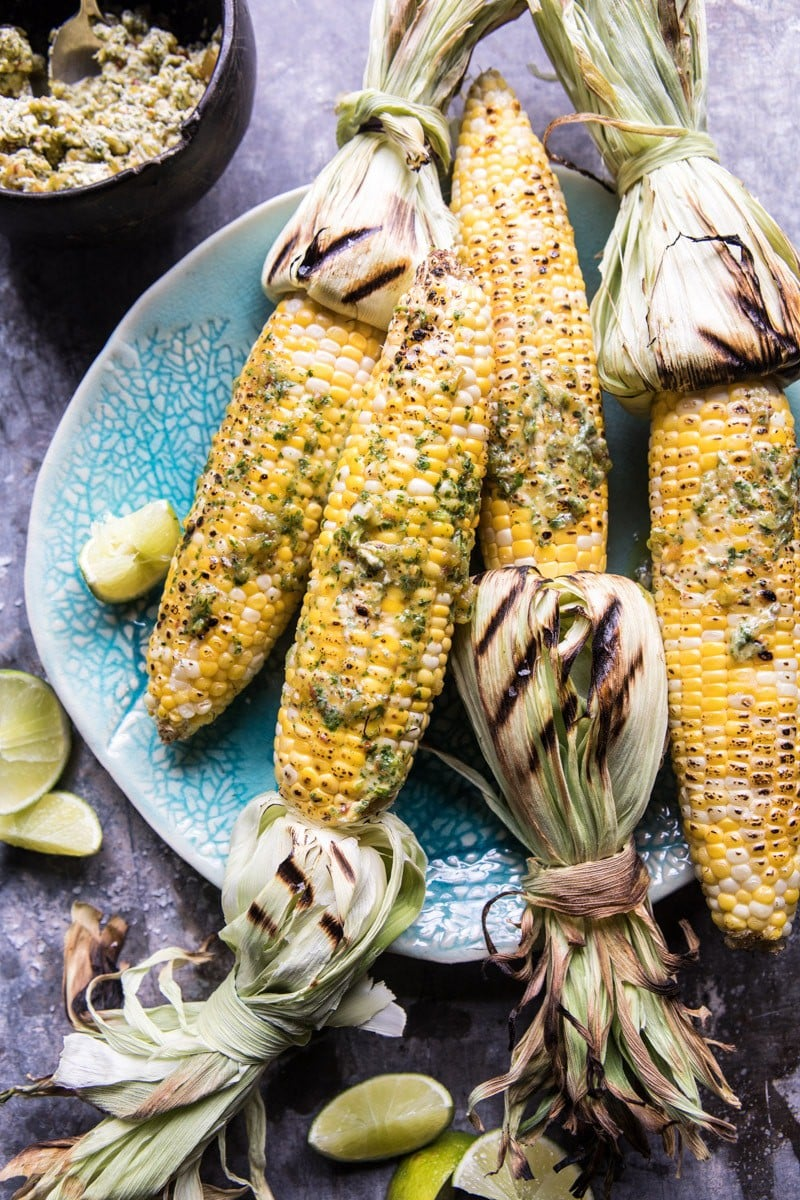
\includegraphics[width=1\textwidth,height=\textheight]{images/mexican-grilled-corn-with-green-chile-honey-butter.jpg}

\textbf{Prep Time:} 10 min \textbar{} \textbf{Cook Time:} 20 min
\textbar{} \textbf{Total Time:} 30 min

\section{Ingredients}\label{ingredients-91}

\begin{itemize}
\tightlist
\item
  6 ears corn
\item
  1 stick (8 tablespoons) unsalted butter
\item
  1 4.5 ounce can Old El Paso Chopped Green Chiles, drained
\item
  1 chipotle pepper in adobo
\item
  1/4 cup fresh cilantro
\item
  2 teaspoons honey
\item
  1/2 teaspoon ground cumin
\item
  1 teaspoon kosher salt, plus more if needed
\end{itemize}

\section{Instructions}\label{instructions-91}

\begin{enumerate}
\def\labelenumi{\arabic{enumi}.}
\tightlist
\item
  Preheat the grill to medium high heat.
\item
  Pull the outer husks of the corn down to the base and strip away the
  silk. Fold husks back into place to cover the kernels.
\item
  Grill for about 5 minutes on each “side” – rotating corn 4-5 times.
  Once the corn is finished, remove the husk and place back on the grill
  until lightly charred, about 5 more minutes.
\item
  Meanwhile, add the butter, chopped green chiles, chipotle pepper in
  adobo, cilantro, honey, cumin, and a large pinch of salt to the bowl
  of a food processor and pulse until combined.
\item
  Spread the butter over the warm corn. Serve with salt, cilantro, and
  limes. Eat!
\end{enumerate}

\bookmarksetup{startatroot}

\chapter{Spicy Maple Grilled Chicken Sandwich with Smoky Bacon
Corn}\label{spicy-maple-grilled-chicken-sandwich-with-smoky-bacon-corn}

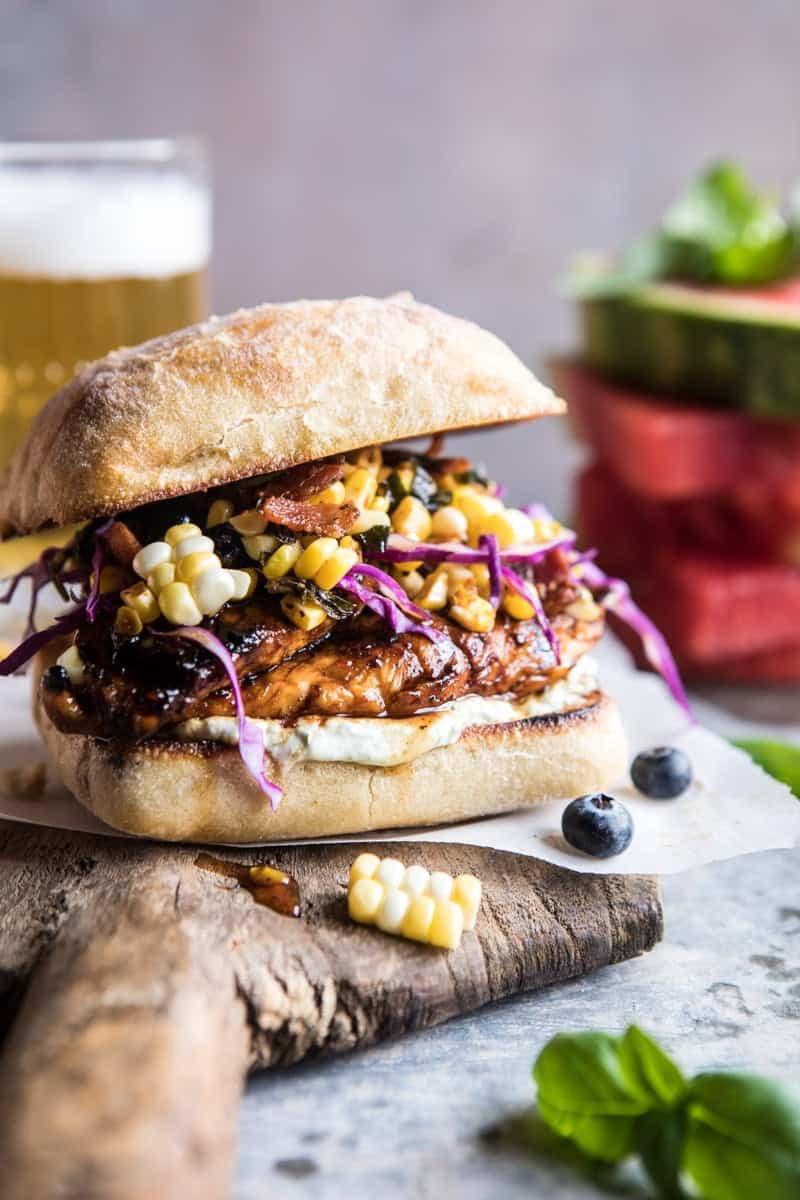
\includegraphics[width=1\textwidth,height=\textheight]{images/spicy-maple-grilled-chicken-sandwich-with-smoky-bacon-corn.jpg}

\textbf{Prep Time:} 10 min \textbar{} \textbf{Cook Time:} 20 min
\textbar{} \textbf{Total Time:} 30 min

\section{Ingredients}\label{ingredients-92}

\begin{itemize}
\tightlist
\item
  1/2 cup real maple syrup
\item
  1 tablespoon sambal oelek ((spicy chili sauce))
\item
  2 tablespoons extra virgin olive oil
\item
  kosher salt and pepper
\item
  1 pound boneless skinless chicken tenders
\item
  4 slices thick cut bacon, chopped
\item
  4 ears corn, kernels removed from the cob ((about 4 cups total))
\item
  1 teaspoon smoked paprika
\item
  1/4 cup fresh basil, chopped
\item
  2 green onions, chopped
\item
  1/2 cup shredded cabbage
\item
  1/2 cup fresh blueberries
\item
  4 ciabatta rolls, toasted
\item
  1/2 cup plain greek yogurt
\item
  1/4 cup basil pesto
\item
  1 avocado, sliced
\end{itemize}

\section{Instructions}\label{instructions-92}

\begin{enumerate}
\def\labelenumi{\arabic{enumi}.}
\tightlist
\item
  Stir together the maple syrup, sambal oelek, olive oil, and a pinch of
  salt in a small bowl. Add the chicken to a large ziplock bag and pour
  half the maple mixture over the chicken. Let sit for 10 minutes.
\item
  Meanwhile, heat a large skillet over medium heat and cook the bacon
  until crisp, about 5-8 minutes. Stir in the corn, paprika, and pinch
  each of salt and pepper. Cook 5 minutes and then add the basil, and
  green onions. Remove from the heat and let cool slightly. Stir in the
  cabbage and blueberries.
\item
  Preheat an outdoor grill or grill pan to medium heat. Oil the grates.
\item
  Add the chicken and grill for 5-8 minutes per side, basting the
  chicken with the reserve maple mixture until the chicken is cooked
  through. Remove from the grill and drizzle any remaining maple mix
  over the chicken.
\item
  Mix the yogurt and pesto together in a small bowl.
\item
  To assemble, spread the yogurt pesto mix onto the bottom of each bun.
  Top with chicken, corn, and avocado. EAT!
\end{enumerate}

\bookmarksetup{startatroot}

\chapter{Brunch Bruschetta Bar}\label{brunch-bruschetta-bar}

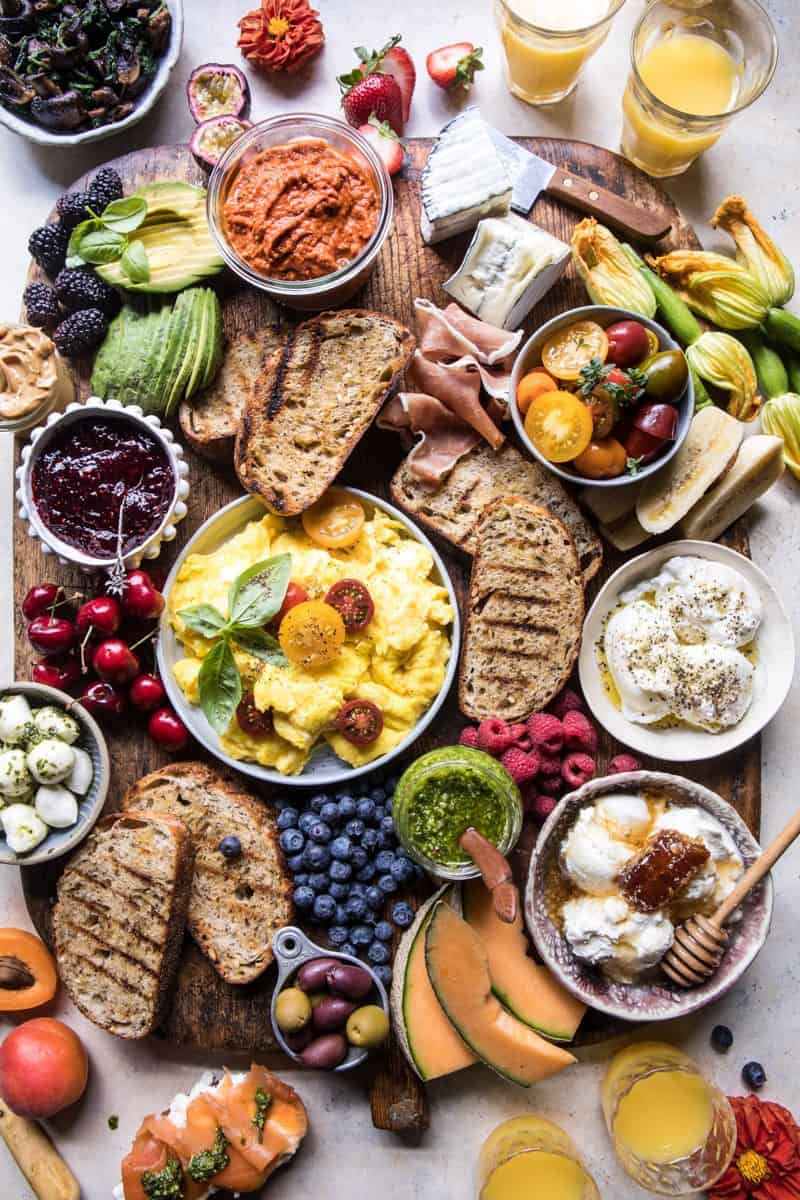
\includegraphics[width=1\textwidth,height=\textheight]{images/brunch-bruschetta-bar.jpg}

\textbf{Prep Time:} 15 min \textbar{} \textbf{Cook Time:} \textbar{}
\textbf{Total Time:} 15 min

\section{Ingredients}\label{ingredients-93}

\begin{itemize}
\tightlist
\item
  1 batch basil pesto
\item
  1 batch Sun-Dried Tomato Muhammara ((tomato and roasted red pepper
  spread))
\item
  1 batch marinated cherry tomatoes or 2 cups tomatoes
\item
  6-8 soft-boiled or poached eggs
\item
  6-8 scrambled eggs
\item
  6-8 pieces fried bacon
\item
  2-3 cheeses ((I used Humboldt Fog goat cheese, ricotta and marinated
  mozzarella))
\item
  grilled or toasted bread
\item
  sautéed veggies, such as spinach and mushrooms
\item
  fresh fruits
\item
  sliced avocado
\item
  prosciutto, salami, and smoked salmon
\item
  raspberry jam or other fruit jams
\item
  nut butter
\item
  honey or honeycomb
\item
  • not-from-concentrate Florida's Natural® Brand Orange Juice
\end{itemize}

\section{Instructions}\label{instructions-93}

\begin{enumerate}
\def\labelenumi{\arabic{enumi}.}
\tightlist
\item
  Arrange the sauces and spreads on a large serving board. Add the
  poached eggs, scrambled eggs, and bread. Drizzle the poached eggs with
  olive oil and season with salt and pepper. Arrange the cheese, fruits,
  veggies, meats, jams, nut butter, and honey around the eggs.
\item
  Pour Florida’s Natural orange juice into juice glasses for sipping.
  Enjoy!
\end{enumerate}

\bookmarksetup{startatroot}

\chapter{Garden Fresh Herb, Olive, and Parmesan Pasta with Pistachio
Breadcrumbs}\label{garden-fresh-herb-olive-and-parmesan-pasta-with-pistachio-breadcrumbs}

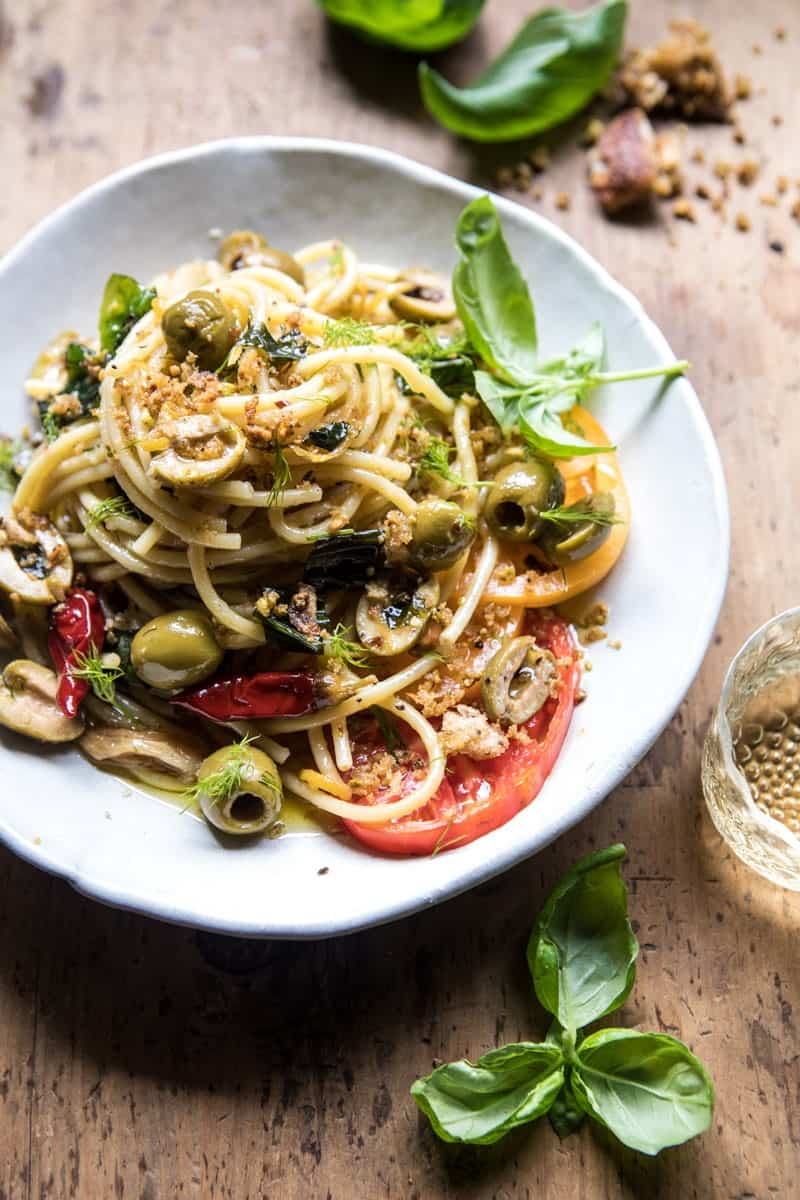
\includegraphics[width=1\textwidth,height=\textheight]{images/garden-fresh-herb-olive-and-parmesan-pasta-with-pistachio-breadcrumbs.jpg}

\textbf{Prep Time:} 10 min \textbar{} \textbf{Cook Time:} 20 min
\textbar{} \textbf{Total Time:} 30 min

\section{Ingredients}\label{ingredients-94}

\begin{itemize}
\tightlist
\item
  2 cups roughly torn ciabatta bread
\item
  1/4 cup shelled roasted pistachios
\item
  1/2 cup olive oil
\item
  4 cloves garlic, smashed
\item
  1-3 teaspoons crushed red pepper flakes or 2-3 chili peppers ((use to
  your taste))
\item
  2 sprigs fresh oregano
\item
  2 sprigs fresh thyme
\item
  the rind of one lemon, thinly sliced
\item
  kosher salt and pepper
\item
  1 cup pitted green olives, halved
\item
  1 pound bucatini pasta or other long cut pasta
\item
  1/4 cup white wine
\item
  1 cup fresh grated parmesan
\item
  1/4 cup fresh basil, chopped
\item
  2 tablespoons fresh dill, chopped
\item
  2 sliced tomatoes or 1 cup cherry tomatoes, for serving
\end{itemize}

\section{Instructions}\label{instructions-94}

\begin{enumerate}
\def\labelenumi{\arabic{enumi}.}
\tightlist
\item
  Preheat the oven to 375 degrees F.
\item
  On a baking sheet, combine the bread crumbs, pistachios, 2 tablespoons
  olive oil, and large pinch of both salt and pepper. Toss well to coat.
  Transfer to the oven and cook 8-10 minutes or until the breadcrumbs
  are golden. Remove from the oven.
\item
  To a large skillet with sides, add the remaining olive oil (about 1/3
  cup), the crushed red pepper flakes, garlic, oregano, thyme, lemon
  rind, and a pinch each of salt and pepper. Set over medium heat and
  cook, stirring occasionally for 10 minutes or until the garlic is
  caramelized and fragrant. Reduce the heat to low and then stir in the
  olives and cook another 5 minutes.
\item
  Meanwhile, bring a large pot of salted water to a boil. Add the pasta
  and cook according to package directions until al dente. Just before
  draining, remove 1 cup of the pasta cooking water. Drain.
\item
  Add the hot pasta right into the skillet with oil and seasonings. Add
  the wine and toss to combines. Cook for 5 minutes. Remove from the
  heat and add the parmesan, basil, and dill, tossing to combine. If
  needed, thin the pasta with a little of the reserve cooking water.
\item
  Divide the pasta among each plate. Top with tomatoes, breadcrumbs and
  fresh basil. EAT.
\end{enumerate}

\bookmarksetup{startatroot}

\chapter{Strawberry Melon Elderflower Pimms
Cup}\label{strawberry-melon-elderflower-pimms-cup}

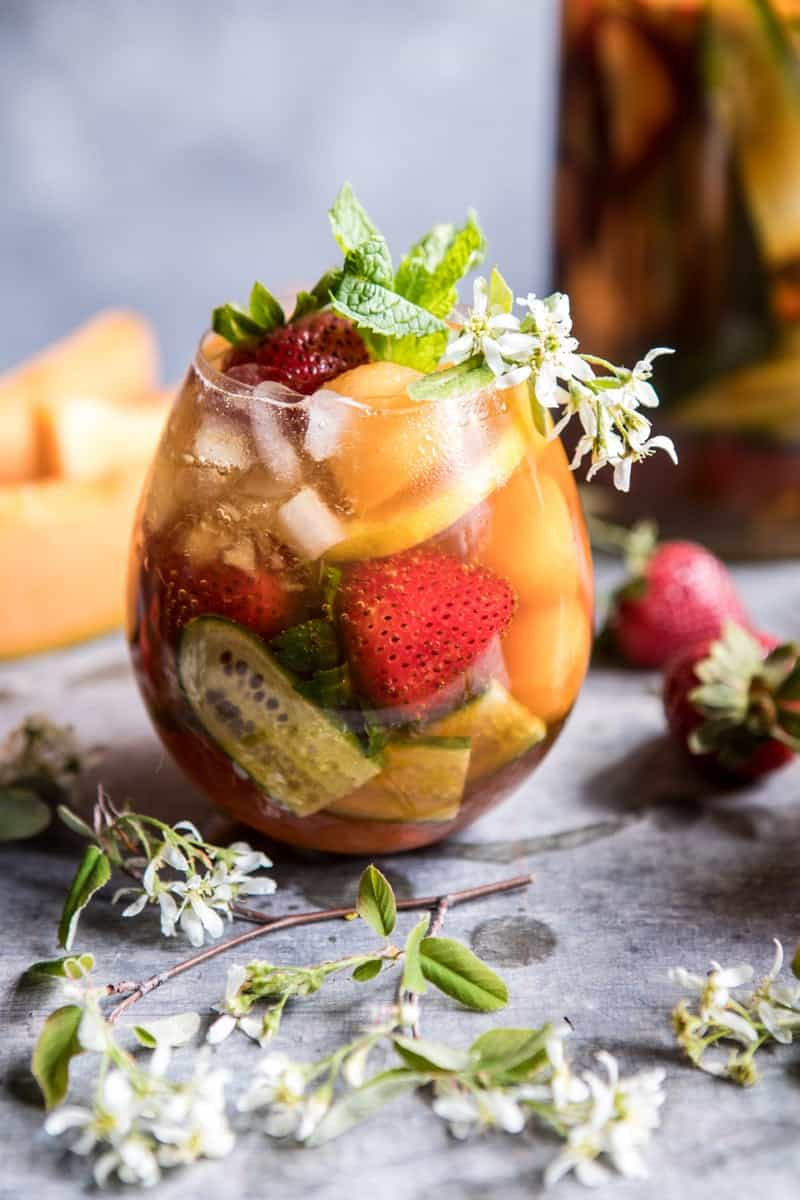
\includegraphics[width=1\textwidth,height=\textheight]{images/strawberry-melon-elderflower-pimms-cup.jpg}

\textbf{Prep Time:} 5 min \textbar{} \textbf{Cook Time:} \textbar{}
\textbf{Total Time:} 5 min

\section{Ingredients}\label{ingredients-95}

\begin{itemize}
\tightlist
\item
  4 cucumber slices
\item
  2 strawberries sliced
\item
  4 melon balls
\item
  2-3 lemons slices
\item
  3 ounces Pimms No 1
\item
  1 1/2 ounces Elderflower liquor ((St-Germain))
\item
  2 tablespoons lemon juice
\item
  crushed ice
\item
  ginger beer, for topping
\item
  fresh thyme and mint, for serving
\end{itemize}

\section{Instructions}\label{instructions-95}

\begin{enumerate}
\def\labelenumi{\arabic{enumi}.}
\tightlist
\item
  In the bottom of a tall glass, layer the cucumbers, strawberries,
  melon balls, and lemon slices, filling the glass about half way. Pour
  the Pimms, Elderflower liquor, and lemon juice over the cucumbers and
  fruit. Gently stir to combine. Add crushed ice and then top with
  ginger beer. Garnish with thyme and mint. Drink up!
\end{enumerate}

\bookmarksetup{startatroot}

\chapter{Tiramisu Brownie Ice Cream Sandwich
Bars}\label{tiramisu-brownie-ice-cream-sandwich-bars}

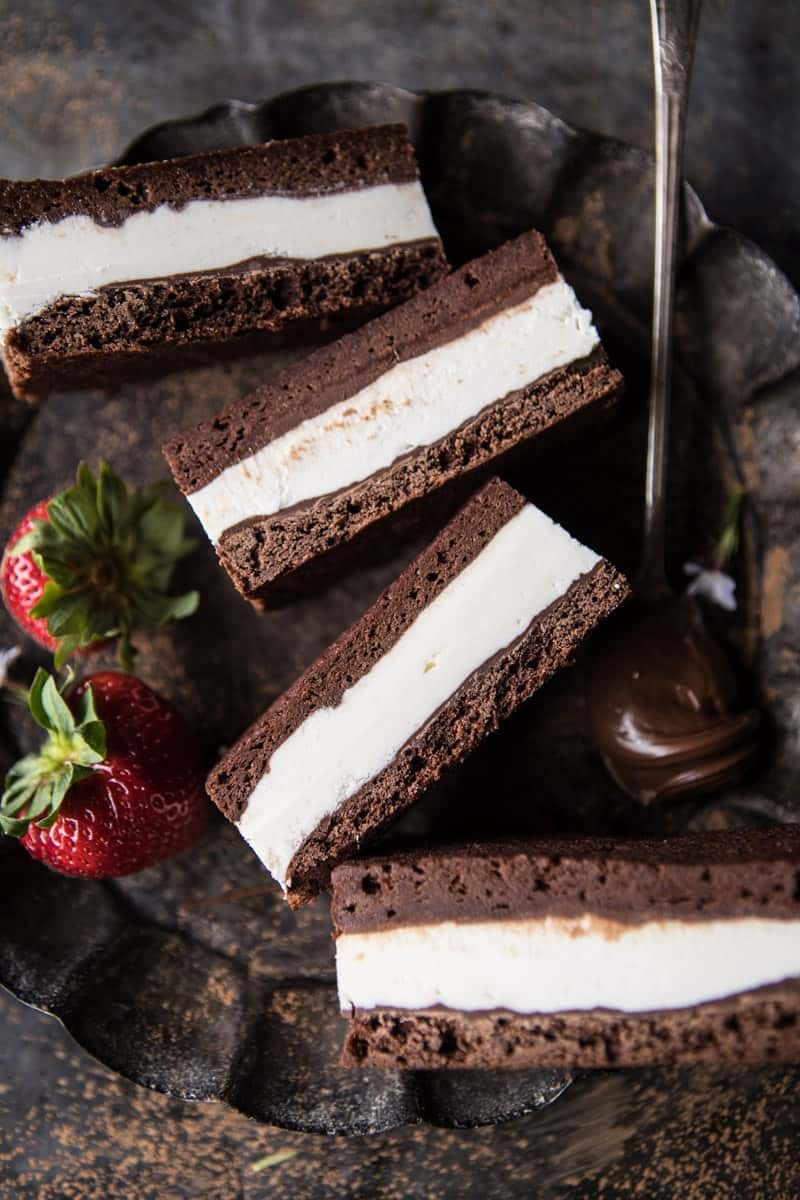
\includegraphics[width=1\textwidth,height=\textheight]{images/tiramisu-brownie-ice-cream-sandwich-bars.jpg}

\textbf{Prep Time:} 20 min \textbar{} \textbf{Cook Time:} 10 min
\textbar{} \textbf{Total Time:} 6 hr

\section{Ingredients}\label{ingredients-96}

\begin{itemize}
\tightlist
\item
  1 stick (1/2 cup) unsalted butter
\item
  2 ounces chocolate, milk or dark, chopped
\item
  3/4 cup granulated sugar
\item
  2 teaspoons vanilla extract
\item
  1-2 tablespoons instant coffee granules
\item
  2 large eggs
\item
  1/2 cup unsweetened cocoa powder
\item
  1/2 cup all-purpose flour
\item
  1/4 teaspoon kosher salt
\item
  1/2 cup Nutella
\item
  4 ounces mascarpone cheese
\item
  1/2 cup sweetened condensed milk
\item
  1 cup heavy cream
\item
  1 teaspoon vanilla
\item
  pinch of flaky sea salt
\end{itemize}

\section{Instructions}\label{instructions-96}

\begin{enumerate}
\def\labelenumi{\arabic{enumi}.}
\tightlist
\item
  Preheat the oven to 350 degrees F. Line two (8x8 inch) square baking
  pans with parchment paper.
\item
  Add the butter and chocolate to a medium size, microwave safe, mixing
  bowl. Microwave on high for 30 second intervals, stirring after each
  interval, until melted and smooth. To the melted chocolate whisk in
  the sugar, vanilla, coffee, and eggs until smooth. Stir in the cocoa
  powder, flour and salt until just combined, try not to over mix the
  batter. It will be thick. Divide the batter evenly into the prepared
  pans, spreading it in an even layer, the layers will be thin. Transfer
  to the oven and bake for 10-12 minutes, until the brownies are set on
  top. Remove from the oven and allow to cool completely.
\item
  Once cooled, spread the Nutella evenly onto each brownie pan.
\item
  To make the ice cream. Add the mascarpone and sweetened condensed milk
  to the bowl of a stand mixer fitted with the whisk attachment (or use
  a hand held electric mixer) and whip until smooth and combined. Add
  the heavy cream, vanilla and salt. Whip until stiff peaks form.
\item
  Spread the ice cream in an even layer over top one of the brownie
  pans. It's easiest if you keep the brownie in the parchment lined
  square baking pan. Then place the other brownie gently on top of the
  ice cream, Nutella side facing down. Cover with plastic wrap and
  freeze for 4-6 hours or overnight.
\item
  Slice bars into rectangles and keep stored in the freezer for up to a
  couple months.
\end{enumerate}

\bookmarksetup{startatroot}

\chapter{Cheesy Zucchini Roasted Corn Tacos With Mango Salsa
Verde}\label{cheesy-zucchini-roasted-corn-tacos-with-mango-salsa-verde}

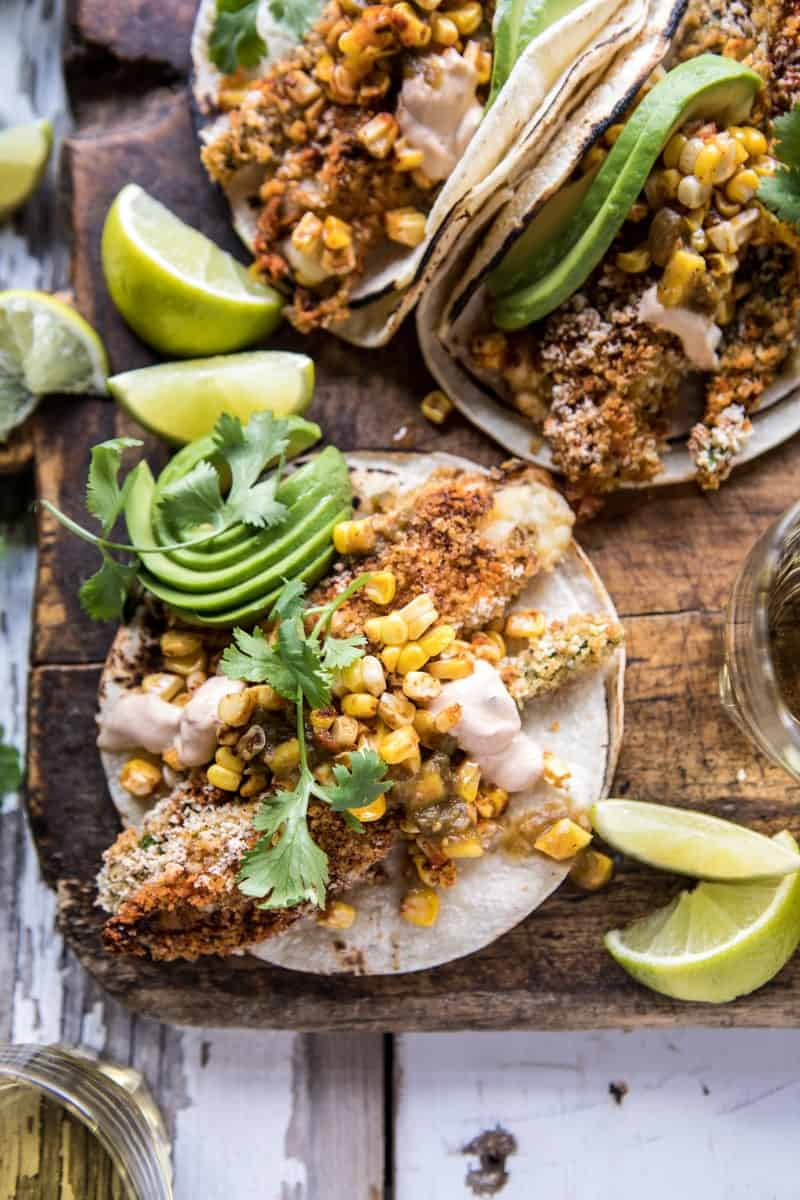
\includegraphics[width=1\textwidth,height=\textheight]{images/cheesy-zucchini-roasted-corn-tacos-with-mango-salsa-verde.jpg}

\textbf{Prep Time:} 15 min \textbar{} \textbf{Cook Time:} 15 min
\textbar{} \textbf{Total Time:} 30 min

\section{Ingredients}\label{ingredients-97}

\begin{itemize}
\tightlist
\item
  12 zucchini blossoms OR 2-3 zucchini sliced into quarters longways
\item
  1 1/2 cups shredded pepper jack or cheddar cheese
\item
  2 eggs
\item
  1 1/2 cups panko bread crumbs
\item
  3 tablespoons whole wheat or all-purpose flour
\item
  2 teaspoons chili powder
\item
  2 teaspoons paprika
\item
  kosher salt and pepper
\item
  2 cups fresh corn (about 3 ears)
\item
  2 tablespoons olive oil, plus more for brushing
\item
  6 corn or flour tortillas, warmed
\item
  fresh cilantro and avocado, for serving
\item
  1 cup salsa verde, homemade or store-bought
\item
  3/4 cup fresh chopped mango
\item
  1 cup plain greek yogurt
\item
  1-2 chipotle peppers in adobo
\item
  juice from 1 lime
\item
  1-2 tablespoons honey
\item
  kosher salt
\end{itemize}

\section{Instructions}\label{instructions-97}

\begin{enumerate}
\def\labelenumi{\arabic{enumi}.}
\tightlist
\item
  Preheat the oven to 425 degrees F. Lightly grease a baking sheet with
  olive oil.
\item
  Grab the zucchini blossoms and carefully open the flowers and stuff
  the insides with about a tablespoon of cheese. Repeat with the
  remaining flowers. If you are using sliced zucchini, skip this step.
\item
  Whisk the eggs in a shallow bowl.
\item
  Add the panko, flour, 1 teaspoon chili powder, 1 teaspoon paprika, and
  a pinch each of salt and pepper, to a separate shallow bowl and toss
  to combine.
\item
  Working with one zucchini or blossom at a time, dip through the eggs
  and then dredge through the panko mix, pressing gently to adhere.
  Place on the prepared baking sheet. Repeat with the remaining
  zucchini, arranging them to one side of the pan. Brush or drizzle the
  tops of the zucchini with olive oil.
\item
  On the same pan, but opposite side, add the corn. and toss with the
  remaining 1 teaspoon chili powder and remaining 1 teaspoon paprika.
  Season with salt and pepper and then toss to combine. Transfer the
  baking sheet to the oven and bake for 15-20 minutes or until the
  blossoms are golden and crisp. If using regular zucchini, sprinkle the
  cheese on during the last 5-10 minutes of cooking to allow it to melt
  over the zucchini.
\item
  Meanwhile, make the salsa. In a small bowl, stir together the salsa
  verde and mango.
\item
  To serve, divide the zucchini among warmed tortillas and top with
  corn, avocado, salsa, and cream. EAT.
\end{enumerate}

\bookmarksetup{startatroot}

\chapter{Burst Cherry Tomato, Artichoke, and Zucchini Pesto
Pizza}\label{burst-cherry-tomato-artichoke-and-zucchini-pesto-pizza}

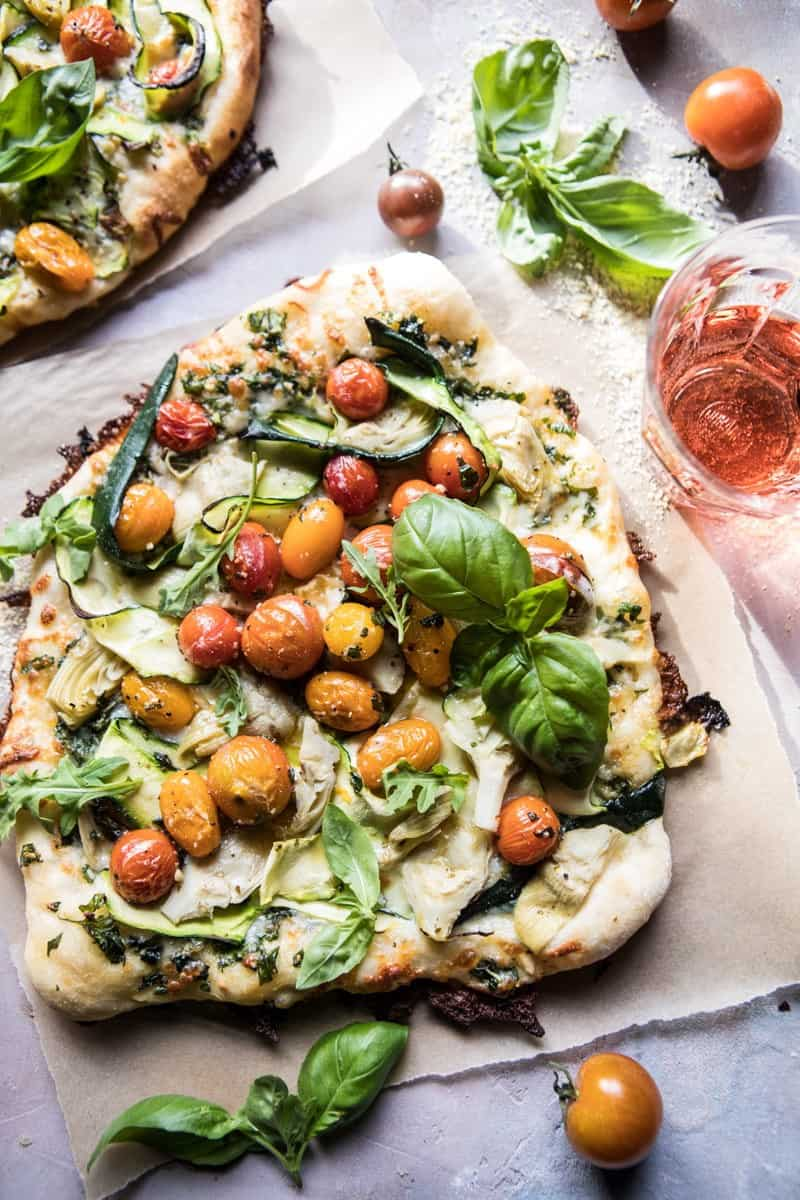
\includegraphics[width=1\textwidth,height=\textheight]{images/burst-cherry-tomato-artichoke-and-zucchini-pesto-pizza.jpg}

\textbf{Prep Time:} 15 min \textbar{} \textbf{Cook Time:} 15 min
\textbar{} \textbf{Total Time:} 30 min

\section{Ingredients}\label{ingredients-98}

\begin{itemize}
\tightlist
\item
  1/2 pound pizza dough, homemade or store-bought
\item
  1 cup basil pesto, homemade or store-bought
\item
  1 cup shredded provolone cheese
\item
  1 cup shredded mozzarella cheese
\item
  1 medium-sized zucchini, cut into ribbons
\item
  1 (12 ounce) jar marinated artichokes hearts, drained
\item
  2 cups cherry tomatoes
\item
  2 tablespoons olive oil
\item
  1 clove garlic, minced or grated
\item
  1 tablespoon chopped fresh thyme
\item
  kosher salt and pepper
\item
  pinch of crushed red pepper flakes
\item
  fresh basil and arugula for topping
\end{itemize}

\section{Instructions}\label{instructions-98}

\begin{enumerate}
\def\labelenumi{\arabic{enumi}.}
\tightlist
\item
  Preheat the oven to 450 degrees F. Grease a large baking sheet with
  olive oil.
\item
  On a lightly floured surface, push/roll the dough out until until it
  is pretty thin (about a 10-12 inch circle). Transfer the dough to the
  prepared baking sheet. Spread the dough with pesto and top with
  provolone and mozzarella. Add the zucchini and artichokes, you might
  not need all the artichokes. Add the tomatoes to a bowl and toss with
  the olive oil, garlic, thyme, salt and pepper. Spoon the tomatoes over
  pizza, drizzling any oil left in the bowl over the pizza as well.
\item
  Transfer to the oven and bake for 10-15 minutes or until the crust is
  golden, the cheese has melted and the tomatoes have burst. Remove from
  the oven and top with fresh basil and arugula. Slice and eat!
\end{enumerate}

\bookmarksetup{startatroot}

\chapter{Grilled Corn and Feta Egg in a Hole Avocado
Toast}\label{grilled-corn-and-feta-egg-in-a-hole-avocado-toast}

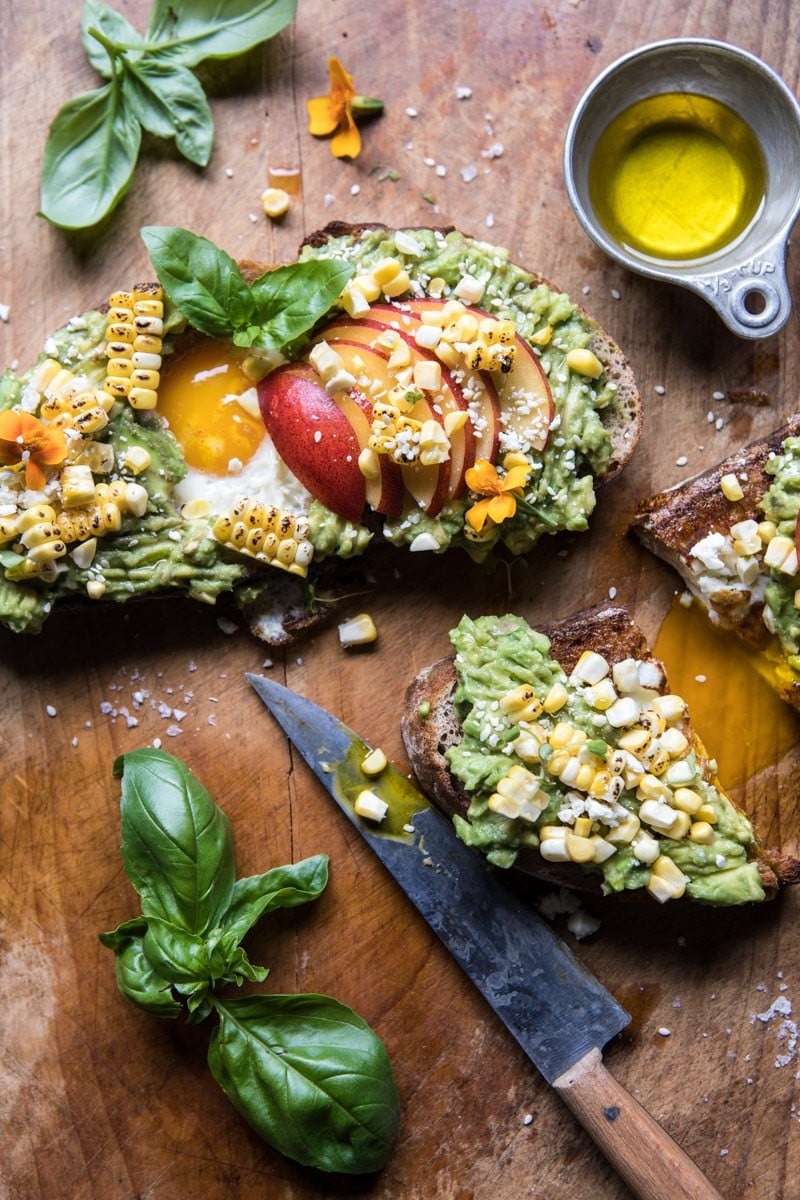
\includegraphics[width=1\textwidth,height=\textheight]{images/grilled-corn-and-feta-egg-in-a-hole-avocado-toast.jpg}

\textbf{Prep Time:} 10 min \textbar{} \textbf{Cook Time:} 5 min
\textbar{} \textbf{Total Time:} 15 min

\section{Ingredients}\label{ingredients-99}

\begin{itemize}
\tightlist
\item
  2 slices crusty whole grain bread
\item
  2 tablespoons olive oil or butter, plus more oil for drizzling
\item
  2 eggs
\item
  flaky sea salt and pepper
\item
  1 avocado, lightly mashed
\item
  juice of 1/2 a lemon
\item
  1 nectarine, thinly sliced
\item
  1 ear charred or grilled corn, kernels removed
\item
  1/3 cup crumbled feta cheese
\item
  crushed red pepper flakes, for topping
\item
  fresh torn basil, for topping
\end{itemize}

\section{Instructions}\label{instructions-99}

\begin{enumerate}
\def\labelenumi{\arabic{enumi}.}
\tightlist
\item
  Using a 2-inch cookie cutter, cut 1 round circle out of each piece of
  bread.
\item
  Heat a large skillet over medium heat and add the olive oil. When the
  oil shimmers, add both the bread and the centers and cook 2-3 minutes
  or until the toast is golden. Flip the toast and crack an egg into the
  center hole of each piece of bread. Season with salt and pepper. Cook
  2-3 minutes and then flip once more and cook 30 seconds to one minutes
  or until the egg is cooked to your liking. Remove from the skillet.
\item
  In a small bowl, mash together the avocado and lemon juice. Season
  with salt. Spread the avocado evenly over each piece of toast. Top
  with nectarines, corn, feta, and basil. Drizzle with olive oil and
  sprinkle with salt. EAT.
\end{enumerate}

\bookmarksetup{startatroot}

\chapter{Strawberry Cornmeal Cake with Buttermilk
Glaze}\label{strawberry-cornmeal-cake-with-buttermilk-glaze}

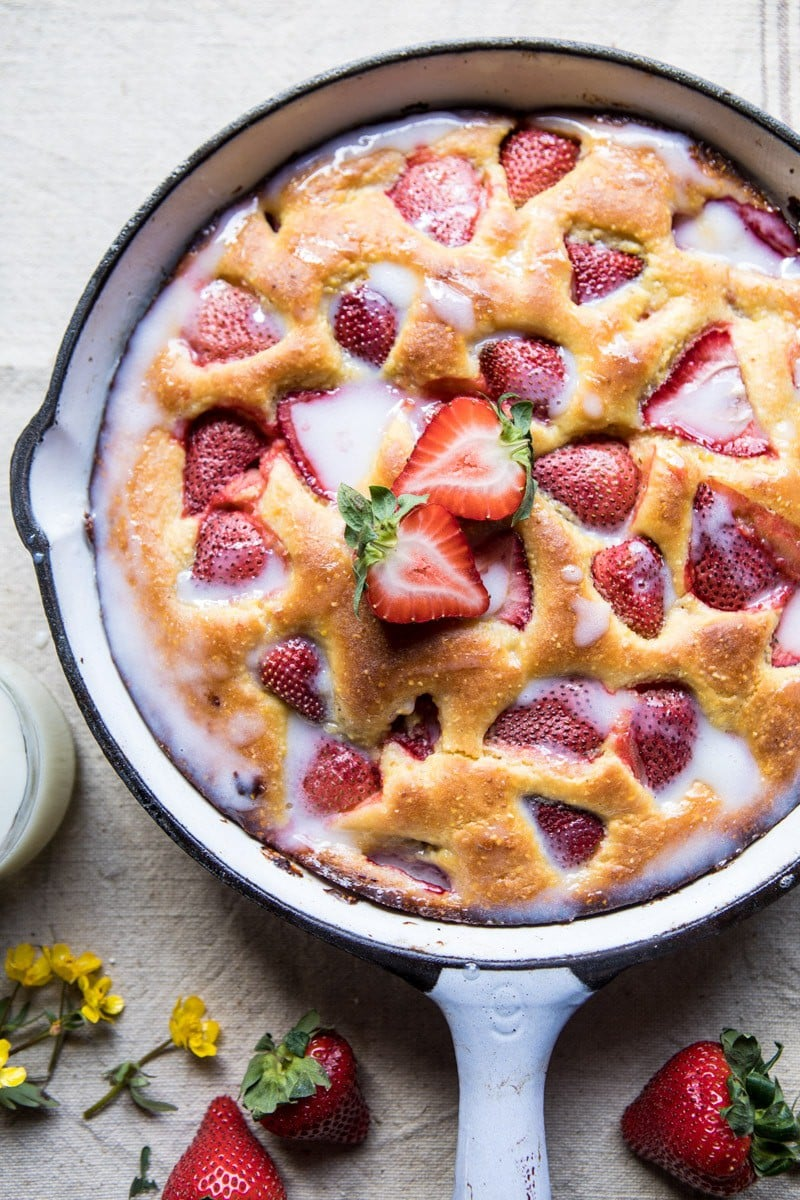
\includegraphics[width=1\textwidth,height=\textheight]{images/strawberry-cornmeal-cake-with-buttermilk-glaze.jpg}

\textbf{Prep Time:} 15 min \textbar{} \textbf{Cook Time:} 30 min
\textbar{} \textbf{Total Time:} 45 min

\section{Ingredients}\label{ingredients-100}

\begin{itemize}
\tightlist
\item
  8 tablespoons unsalted butter, melted
\item
  2 tablespoons light brown sugar
\item
  1/2 cup honey
\item
  1/2 cup buttermilk
\item
  2 teaspoons lemon zest
\item
  2 teaspoons vanilla extract
\item
  2 eggs
\item
  1 1/2 cups Bobs Red Mill all-purpose flour
\item
  3/4 cup Bobs Red Mill Stone Ground Cornmeal
\item
  2 teaspoons baking powder
\item
  1/2 teaspoon kosher salt
\item
  2 cups fresh strawberries, halved
\item
  1/2 cup powdered sugar
\item
  2-4 tablespoons buttermilk
\end{itemize}

\section{Instructions}\label{instructions-100}

\begin{enumerate}
\def\labelenumi{\arabic{enumi}.}
\tightlist
\item
  Preheat the oven to 350 degrees F. Grease one 10-12 inch cast iron
  skillet or cake pan.
\item
  In a large mixing bowl, beat together the butter, brown sugar, honey,
  buttermilk, lemon zest and vanilla until combined about 5 minutes. Add
  the eggs, one at time, beating after each until incorporated. Add the
  flour, cornmeal, baking powder, and salt and beat until combined. Fold
  in the strawberries.
\item
  Pour the batter into the prepared pan.
\item
  Bake for 25-30 minutes or until the cake is golden and a toothpick
  inserted into the center comes out clean. Be careful not to over bake.
\item
  To make the glaze, whisk the powdered sugar and buttermilk together
  until combined.
\item
  Drizzle the glaze over the cake. Slice and serve slightly warm. Enjoy!
\end{enumerate}

\bookmarksetup{startatroot}

\chapter{Lemon and Oregano Grilled
Chicken}\label{lemon-and-oregano-grilled-chicken}

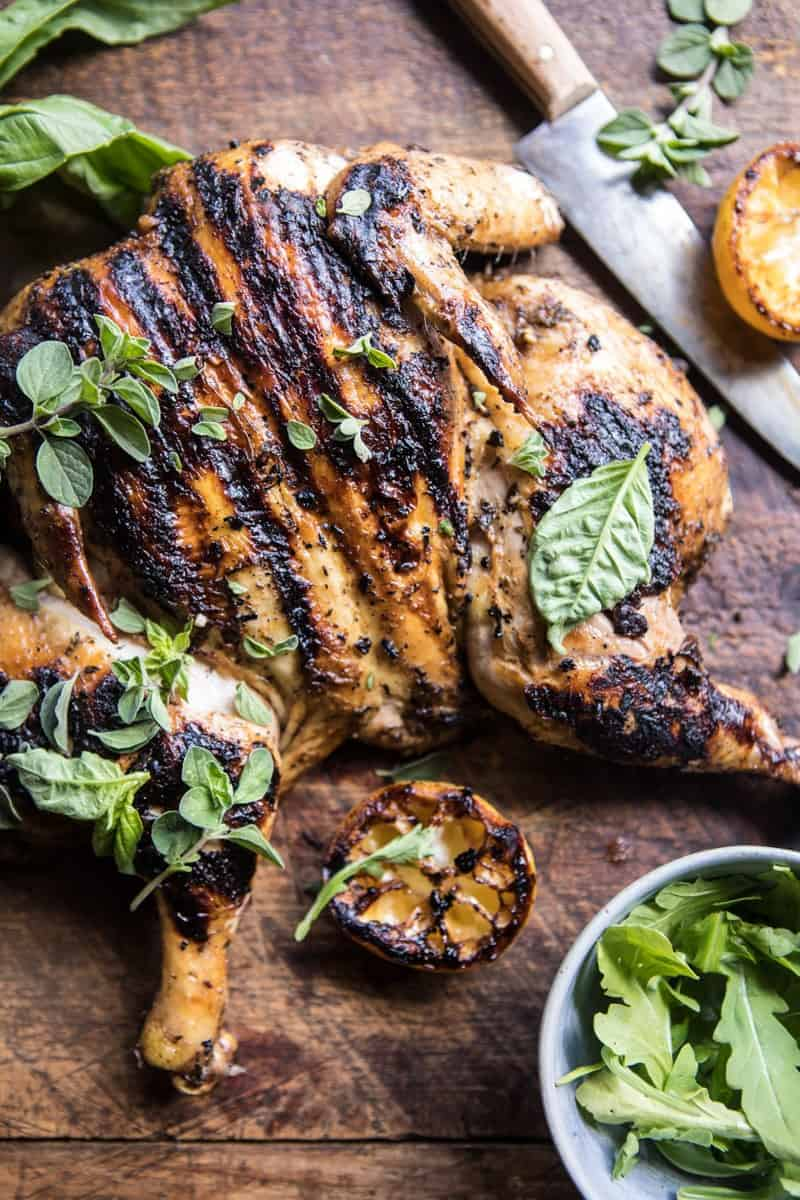
\includegraphics[width=1\textwidth,height=\textheight]{images/lemon-and-oregano-grilled-chicken.jpg}

\textbf{Prep Time:} 15 min \textbar{} \textbf{Cook Time:} 35 min
\textbar{} \textbf{Total Time:} 50 min

\section{Ingredients}\label{ingredients-101}

\begin{itemize}
\tightlist
\item
  1 (3 1/2 to 4 pounds) whole chicken or chicken pieces
\item
  1/4 cup extra virgin olive oil
\item
  3 tablespoons balsamic vinegar
\item
  juice + zest of 1 lemon
\item
  1/4 cup fresh oregano, chopped
\item
  2 tablespoons fresh thyme, chopped
\item
  2 cloves garlic, minced or grated
\item
  pinch of crushed red pepper flakes
\item
  kosher salt and pepper
\item
  fresh basil for, serving
\end{itemize}

\section{Instructions}\label{instructions-101}

\begin{enumerate}
\def\labelenumi{\arabic{enumi}.}
\tightlist
\item
  If using a whole chicken, remove the chicken giblets. Pat the outside
  dry. Place the chicken on a cutting board, breast side down, so that
  the chicken's back is facing up. Using a pair of sharp kitchen
  scissors, cut closely along either side of the backbone. Remove the
  bone and discard. Turn the chicken over so the breast is now facing up
  and press down firmly on the breast and flatten the chicken. Place the
  chicken in a resealable bag.
\item
  In small bowl, whisk together the olive oil, balsamic vinegar, lemon
  zest + juice, oregano, thyme, garlic, and crushed red pepper flakes.
  Pour the marinade over chicken, rubbing the marinade all over the
  chickens skin. Seal the bag and place in the fridge for 1-2 hours or
  preferably over night.
\item
  Preheat an outdoor grill or large grill pan to medium high.
\item
  Season the chicken generously with salt and pepper. Grill, breast side
  down, covered for 10-15 minutes, or until the chicken has a nice char,
  flip and grill another 10-15 minutes. Flip once more and grill until
  cooked through and the chicken registers 160 degrees F on a
  thermometer. Let rest 10 minutes.
\item
  Serve the chicken with fresh melon, basil and oregano. Enjoy!
\end{enumerate}

\bookmarksetup{startatroot}

\chapter{Rainbow Frozen Yogurt Pops}\label{rainbow-frozen-yogurt-pops}

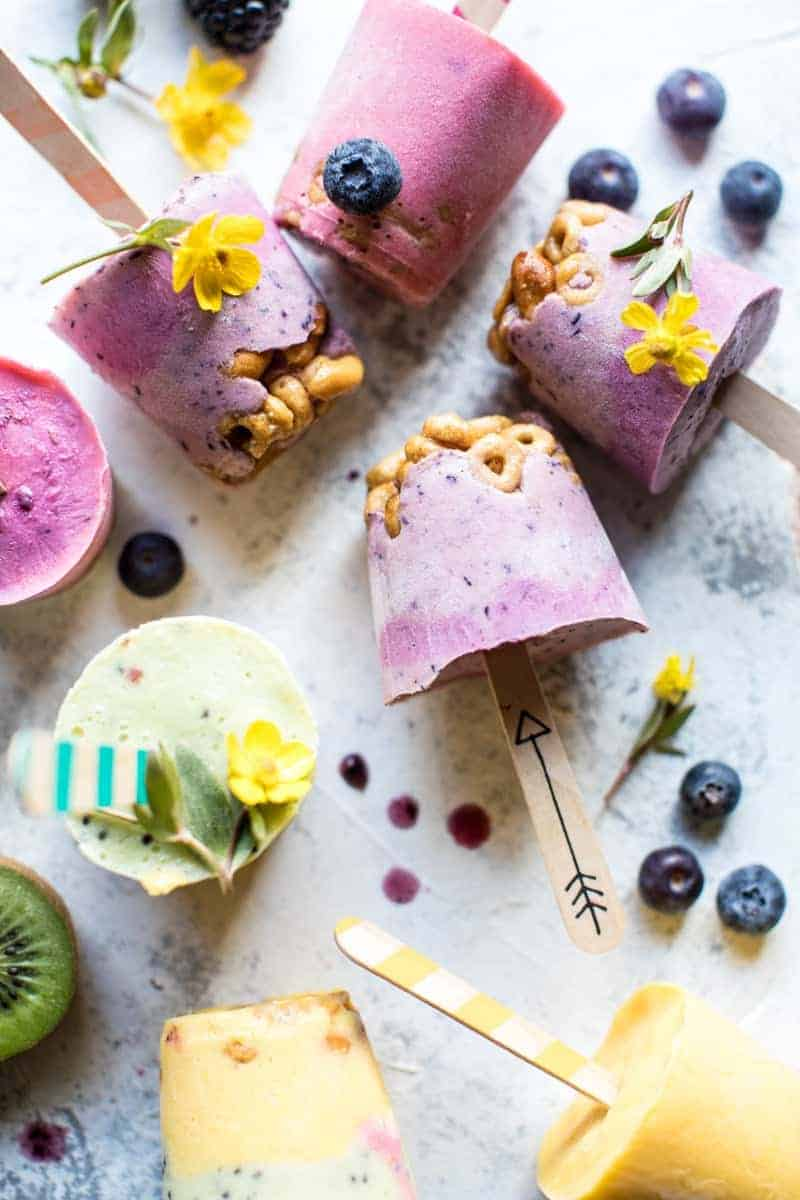
\includegraphics[width=1\textwidth,height=\textheight]{images/rainbow-frozen-yogurt-pops.jpg}

\textbf{Prep Time:} 15 min \textbar{} \textbf{Cook Time:} 15 min
\textbar{} \textbf{Total Time:} 30 min

\section{Ingredients}\label{ingredients-102}

\begin{itemize}
\tightlist
\item
  4 cups plain greek yogurt ((full fat works best))
\item
  1/4 cup honey
\item
  1 teaspoon vanilla extract
\item
  4 cups fresh or frozen fruit (strawberries, blackberries, blueberries,
  raspberries, bananas, pineapple, mangos, kiwi)
\item
  2 cups plain Cheerios
\item
  1 cup rolled oats
\item
  1/2 cup peanuts, roughly chopped
\item
  1/2 cup honey
\item
  3 tablespoons coconut oil or butter
\item
  2 teaspoons vanilla
\end{itemize}

\section{Instructions}\label{instructions-102}

\begin{enumerate}
\def\labelenumi{\arabic{enumi}.}
\tightlist
\item
  In a blender, combine 1 cup of yogurt, 1 tablespoon honey, 1/4
  teaspoon vanilla, and 1 cup of fruit, blend until smooth and creamy.
  Repeat this process with the remaining yogurt and fruit to create your
  desired rainbow colors.
\item
  To assemble, layer the granola (recipe follows) and yogurt evenly
  among 16 popsicles molds or paper dixie cups, creating layers with the
  colors of yogurt, if desired. Insert popsicles sticks and then cover
  the tops and freeze until firm, about 4 hours. To remove the popsicles
  run the mold under hot water for 10 seconds and then pull the
  popsicles out of the molds. Store in the freezer.
\end{enumerate}

\bookmarksetup{startatroot}

\chapter{Buttermilk Pancakes with Chamomile Cream and Gingered
Strawberries}\label{buttermilk-pancakes-with-chamomile-cream-and-gingered-strawberries}

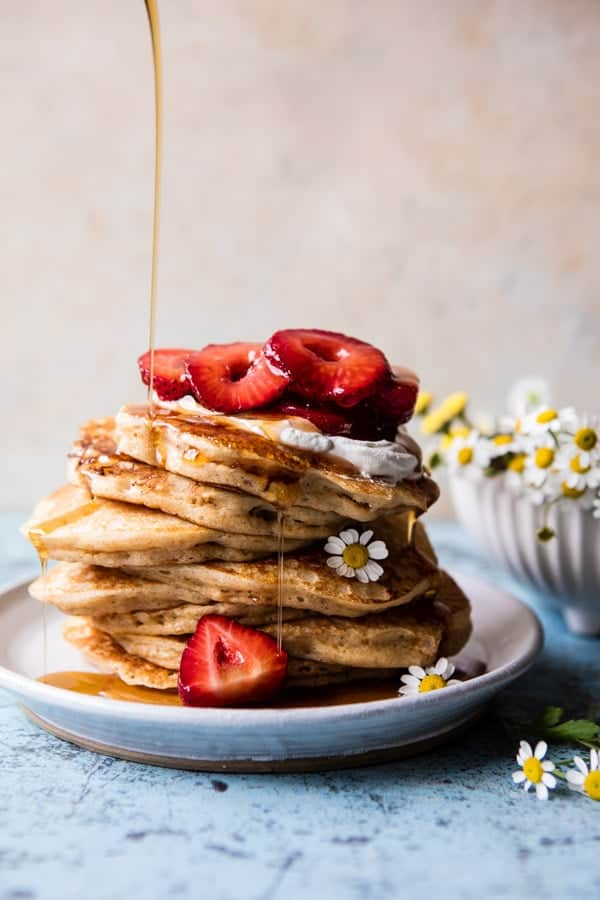
\includegraphics[width=1\textwidth,height=\textheight]{images/buttermilk-pancakes-with-chamomile-cream-and-gingered-strawberries.jpg}

\textbf{Prep Time:} 15 min \textbar{} \textbf{Cook Time:} 15 min
\textbar{} \textbf{Total Time:} 30 min

\section{Ingredients}\label{ingredients-103}

\begin{itemize}
\tightlist
\item
  2 cups all-purpose flour
\item
  2 teaspoons baking powder
\item
  1/2 teaspoon cinnamon
\item
  1/2 teaspoon salt
\item
  1 1/2 cups buttermilk
\item
  1/2 cup plain greek yogurt
\item
  2 eggs
\item
  2 tablespoons melted butter
\item
  1 tablespoon vanilla
\item
  zest from 1 lemon
\item
  1 cup heavy cream
\item
  2 chamomile tea bags
\item
  1 tablespoon honey
\item
  1/4 cup honey
\item
  1 inch fresh ginger grated
\item
  2 cups fresh strawberries sliced
\end{itemize}

\section{Instructions}\label{instructions-103}

\begin{enumerate}
\def\labelenumi{\arabic{enumi}.}
\tightlist
\item
  To make the chamomile cream. Add 1/2 cup cream to a small saucepan and
  bring to a low boil, simmer 1 minute and remove from the heat. Add the
  tea bags, cover and steep for 5-10 minutes. Remove the tea bag and
  place in the fridge to chill completely. Once chilled, add the
  chamomile cream and remaining 1/2 cup cream to a mixing bowl and whip
  until stiff peaks form. Stir in the honey. Keep stored in the fridge.
\item
  To make the pancakes. In a large bowl, combine the flour, baking
  powder, cinnamon, and salt. In a small bowl, whisk together the
  buttermilk, yogurt, eggs, butter, vanilla, and lemon zest.
\item
  Pour the wet ingredients into the dry ingredients and mix the batter
  until just combined. It's OK if there are lumps in the batter. Cover
  the batter and set aside for 10 minutes.
\item
  Meanwhile, make the strawberries. Heat the honey and ginger in a small
  saucepan over medium heat until simmering. Let cool 5 minutes. Add the
  strawberries to a bowl and pour the honey over the berries. Toss to
  combine.
\item
  Heat a large skillet or griddle over medium heat and add the butter,
  or spray with cooking spray. Pour about 1/4 cup pancake batter onto
  the center of the hot pan. Cook until bubbles appear on the surface.
  Using a spatula, gently flip the pancake over and cook the other side
  for a minute, or until golden. Repeat with the remaining batter.
\item
  Serve the pancakes topped with the chamomile cream, strawberries, and
  maple syrup if desired. Enjoy!
\end{enumerate}

\bookmarksetup{startatroot}

\chapter{Tuscan Steak with Marinated Cherry
Tomatoes}\label{tuscan-steak-with-marinated-cherry-tomatoes}

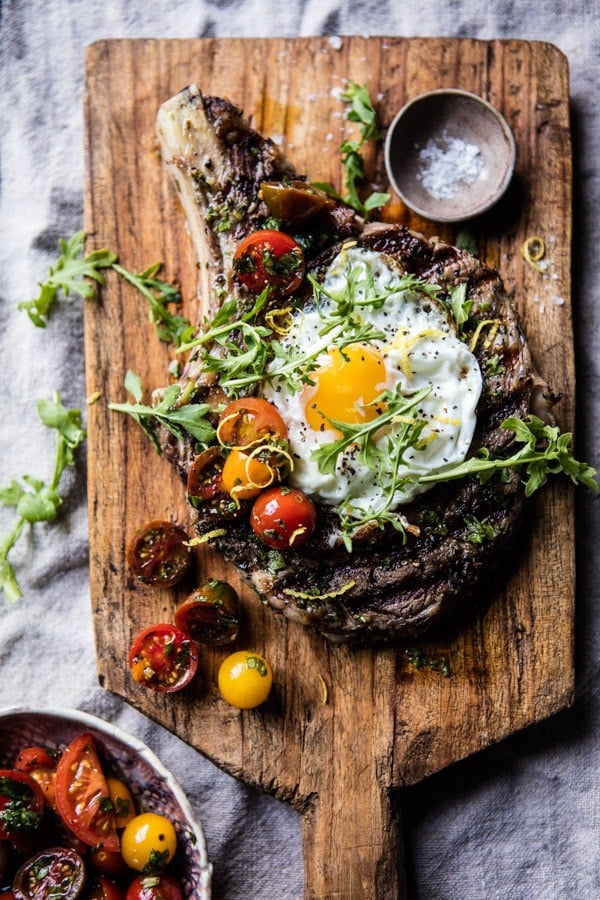
\includegraphics[width=1\textwidth,height=\textheight]{images/tuscan-steak-with-marinated-cherry-tomatoes.jpg}

\textbf{Prep Time:} 15 min \textbar{} \textbf{Cook Time:} 15 min
\textbar{} \textbf{Total Time:} 1 hr 30 min

\section{Ingredients}\label{ingredients-104}

\begin{itemize}
\tightlist
\item
  2 rib-eye steaks, about 1 1/4 inch thick
\item
  1 tablespoon olive oil
\item
  4 sprigs fresh thyme, finely chopped
\item
  2 sprigs fresh rosemary, finely chopped
\item
  2 cloves garlic, minced or grated
\item
  2 fried eggs
\item
  large handful fresh arugula
\item
  1 batch marinated cherry tomatoes, for serving
\item
  2 tablespoons olive oil
\item
  zest + juice of 1 lemon
\item
  2 teaspoons chopped fresh thyme
\item
  2 teaspoons chopped fresh oregano
\item
  1/2 teaspoon kosher salt and pepper
\end{itemize}

\section{Instructions}\label{instructions-104}

\begin{enumerate}
\def\labelenumi{\arabic{enumi}.}
\tightlist
\item
  Place the steaks in a reusable ziplock bag. Add the olive oil, thyme,
  rosemary, and garlic. Seal the bag and rub the marinade into the
  steaks. Refrigerate 1-2 hours, but preferably overnight.
\item
  Remove the steaks from the fridge 30 minutes prior to grilling.
  Preheat the grill or a grill pan to high heat.
\item
  Season the steaks generously with salt and pepper. Sear until your
  desired doneness is reached, about 5-8 minutes for medium-rare, per
  side.
\item
  Remove the steaks and allow to rest 5 minutes.
\item
  Meanwhile, make the herb oil. In a small bowl, mix together the olive
  oil, lemon juice + zest, thyme, oregano, salt, and pepper.
\item
  To serve, plate the steaks and top with a fried egg, fresh arugula and
  the marinated cherry tomatoes. Drizzle with the herb oil. Enjoy!
\end{enumerate}

\bookmarksetup{startatroot}

\chapter{Easiest Lemon Ricotta Asparagus
Ravioli}\label{easiest-lemon-ricotta-asparagus-ravioli}

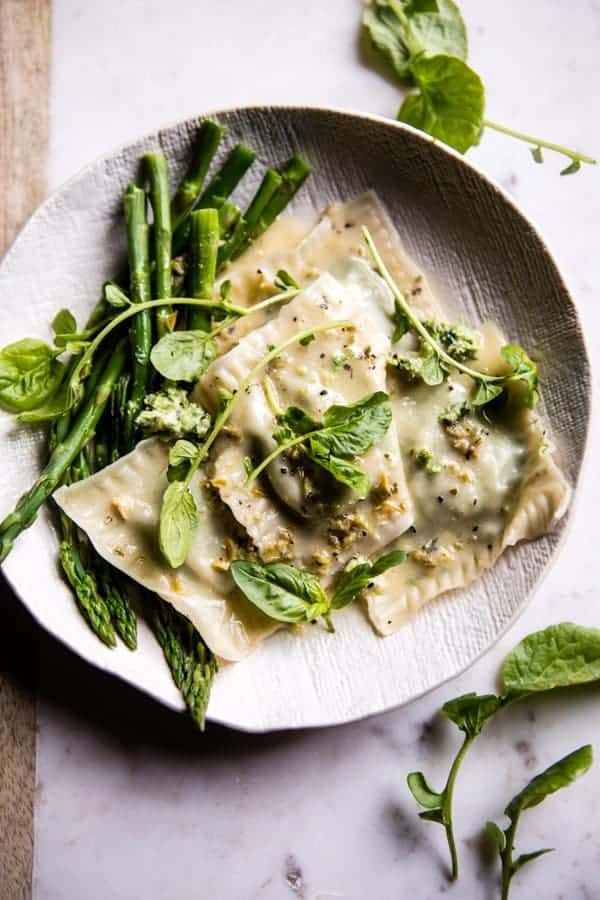
\includegraphics[width=1\textwidth,height=\textheight]{images/easiest-lemon-ricotta-asparagus-ravioli.jpg}

\textbf{Prep Time:} 30 min \textbar{} \textbf{Cook Time:} 15 min
\textbar{} \textbf{Total Time:} 45 min

\section{Ingredients}\label{ingredients-105}

\begin{itemize}
\tightlist
\item
  1 bunch asparagus, ends trimmed
\item
  1 cup fresh basil
\item
  1 cup whole milk ricotta cheese
\item
  1/2 cup grated parmesan cheese
\item
  1/4 cup roasted pistachios, shelloed
\item
  juice + zest of 2 lemons
\item
  kosher salt + pepper
\item
  40-50 circle or square wonton wrappers
\item
  4 tablespoons salted butter
\item
  2 tablespoons chopped chives
\item
  1 tablespoon chopped fresh thyme
\item
  1/2 cup white wine or chicken broth
\item
  1 cup low sodium chicken broth
\item
  pinch of crushed red pepper
\end{itemize}

\section{Instructions}\label{instructions-105}

\begin{enumerate}
\def\labelenumi{\arabic{enumi}.}
\tightlist
\item
  Bring a large pot of salted water to a boil. Add the asparagus and
  blanch until just tender, about 1-2 minutes. Drain and rinse under
  cold water.
\item
  In a food processor, combine 3/4 of the asparagus (reserve the
  remaining for serving), the basil, ricotta, parmesan, pistachios,
  lemon zest and juice, and a pinch each of salt and pepper. Pulse until
  combined and smooth.
\item
  Lay out about 6 wrappers. Spoon 1 tablespoon of filling into the
  center of each wrapper. Brush the edges with water. Lay a second
  wrapper on top of each ravioli. Press down the edges to seal, pressing
  out all the air. Crimp the edges with a fork. Alternately you can
  create triangles with the square wrappers if desired. Be sure to keep
  the ravioli's covered as you work to prevent them from drying out.
\item
  To make the butter sauce. In a large skillet, melt the butter over
  medium heat. Add the chives and thyme and cook 30 seconds to a minute
  or until fragrant. Pour in the wine and chicken broth and bring to a
  boil. Season with salt and pepper and a pinch of crushed red pepper.
  Cook 5 minutes or until the sauce has reduced slightly.
\item
  Meanwhile, bring a large pot of salted water to a boil. Boil the
  ravioli in batches for 1-2 minutes or until they float. Drain.
\item
  Divide the ravioli among bowls and ladle the sauce over the ravioli.
  Top with the remaining asparagus. EAT!
\end{enumerate}

\bookmarksetup{startatroot}

\chapter{Layered Zebra Mousse Cake}\label{layered-zebra-mousse-cake}

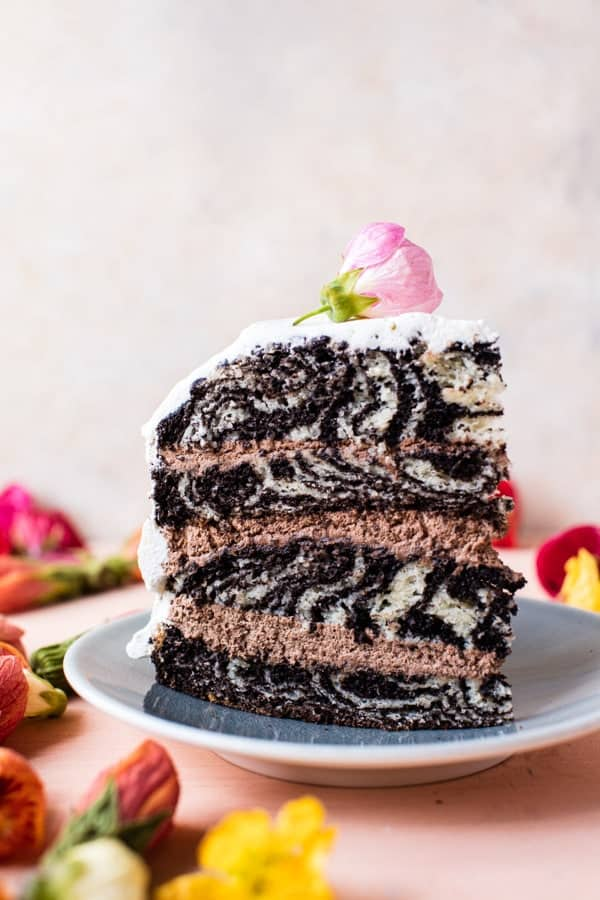
\includegraphics[width=1\textwidth,height=\textheight]{images/layered-zebra-mousse-cake.jpg}

\textbf{Prep Time:} 25 min \textbar{} \textbf{Cook Time:} 35 min
\textbar{} \textbf{Total Time:} 1 hr

\section{Ingredients}\label{ingredients-106}

\begin{itemize}
\tightlist
\item
  4 cups all-purpose flour
\item
  1 tablespoon baking powder
\item
  2 teaspoons kosher salt
\item
  2 cups buttermilk
\item
  1/4 cup plain greek yogurt
\item
  1 cup canola oil
\item
  4 eggs
\item
  2 cups granulated sugar
\item
  1 tablespoon vanilla extract
\item
  1/2 cup unsweetened cocoa powder
\item
  1/4 cup black coffee
\item
  4 cups heavy whipping cream
\item
  1/2 cup unsweetened cocoa powder
\item
  1/3-1/2 cup honey or powdered sugar
\item
  2 teaspoons vanilla extract
\item
  pinch of sea salt
\end{itemize}

\section{Instructions}\label{instructions-106}

\begin{enumerate}
\def\labelenumi{\arabic{enumi}.}
\tightlist
\item
  Preheat the oven to 350 degrees F. Grease 2 (8 inch) round cake pans.
\item
  In a large bowl, mix together the flour, baking powder, and salt.
\item
  In the bowl of a stand mixer (or use a hand held mixer) beat together
  the buttermilk, greek yogurt, canola oil, eggs, sugar, and vanilla
  until smooth. Slowly add the dry ingredients to the wet ingredients
  with the mixer on low until there are no longer any clumps of flour.
  Batter should be pourable, but not super thin.
\item
  Divide the batter in half. Set one batter aside. To the other batter,
  add the cocoa powder and coffee, beating until smooth.
\item
  Spoon about 1/4 cup of vanilla batter (the one set aside) into the
  center of each prepared 8 inch pan. Now spoon 1/4 cup chocolate batter
  directly over the vanilla batter. Repeat this process, always spooning
  the batter into the center of the pan. It helps to tap the pans
  against the center every so often to evenly distribute the batter.
  Don't stress if things looks a little uneven.
\item
  Transfer to the oven and bake for 35-40 minutes or until a toothpick
  inserted into the center comes out clean. Let cool 5 minutes and then
  invert the cakes onto a wire rack to cool completely.
\item
  Meanwhile, make the mousse. Add 3 cups heavy cream to the bowl of a
  stand mixer fitted with the whisk attachment or use a hand held mixer.
  Whisk the cream until stiff peaks form. Add the cacao powder, honey,
  and vanilla and stir until combined and creamy. Cover and place in the
  fridge.
\item
  To assemble. Using a serrated knife, slice the cakes in half
  horizontally. Place one cake layer on a cake stand and spread with
  mousse. Add another layer and then more mousse. Continue with the
  remaining 2 layers and mousse.
\item
  Add the remaining 1 cup heavy cream to the bowl of a stand mixer
  fitted with the whisk attachment or use a hand held mixer. Whisk the
  cream until stiff peaks form. Stir in 2 tablespoons honey. Spread the
  whipped cream around the outside of the cake. decorate as desired.
  Cake can be made up to 1 day in advance. Keep stored in the fridge
  until ready to serve.
\end{enumerate}

\bookmarksetup{startatroot}

\chapter{Healthier Oven Fried Sweet Tea Buffalo Chicken
Sandwich.}\label{healthier-oven-fried-sweet-tea-buffalo-chicken-sandwich.}

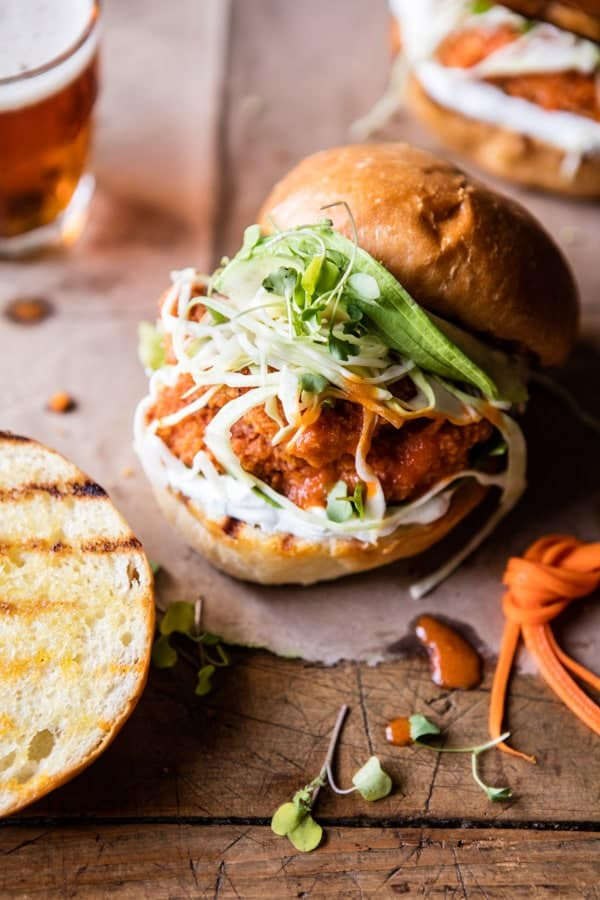
\includegraphics[width=1\textwidth,height=\textheight]{images/healthier-oven-fried-sweet-tea-buffalo-chicken-sandwich-.jpg}

\textbf{Prep Time:} 15 min \textbar{} \textbf{Cook Time:} 30 min
\textbar{} \textbf{Total Time:} 1 hr 45 min

\section{Ingredients}\label{ingredients-107}

\begin{itemize}
\tightlist
\item
  1 1/2 pounds chicken breasts, cut in half widthwise
\item
  3/4 cup buttermilk
\item
  1 1/2 cups sweet green tea
\item
  1 tablespoon kosher salt
\item
  3 cups corn flake crumbs
\item
  3 tablespoons whole wheat flour
\item
  1 tablespoon smoked paprika
\item
  1/2 teaspoon garlic powder
\item
  1 cup buffalo sauce
\item
  8-12 brioche slider buns
\item
  greek yogurt ranch, for serving
\item
  1/4 cup crumbled blue cheese ((optional))
\item
  shredded lettuce, shredded carrots, microgreens, and sliced avocado,
  for serving
\end{itemize}

\section{Instructions}\label{instructions-107}

\begin{enumerate}
\def\labelenumi{\arabic{enumi}.}
\tightlist
\item
  Add the chicken to gallon size zip top bag. Pour the buttermilk, sweet
  tea and salt over the chicken. Toss well, cover and refrigerate 1 hour
  or overnight.
\item
  Preheat the oven to 425 degrees F. Line a baking sheet with parchment.
\item
  Add the corn flakes crumbs, flour, paprika and garlic powder to medium
  sized bowl. Stir to combine.
\item
  Remove each piece of chicken from the buttermilk, and dredge through
  the crumbs, pressing gently to adhere. Place on the prepared baking
  sheet. Repeat until all the chicken has been used. Make sure not to
  crowd your pan, if necessary use two baking sheets. Lightly brush the
  chicken with olive oil. Transfer to the oven and bake for 15-20
  minutes, then flip the chicken over and continue cooking another 10
  minutes or until the chicken is cooked through.
\item
  Drizzle the buffalo sauce over the chicken, covering it almost
  completely.
\item
  To serve, stir the blue cheese into the greek yogurt ranch. Spread the
  greet yogurt on the bottom of each bun. Add the chicken and top with
  veggies and sliced avocado. Serve with buffalo sauce. EAT.
\end{enumerate}

\bookmarksetup{startatroot}

\chapter{Honey Raspberry Brie Crostini with Basil
Oil}\label{honey-raspberry-brie-crostini-with-basil-oil}

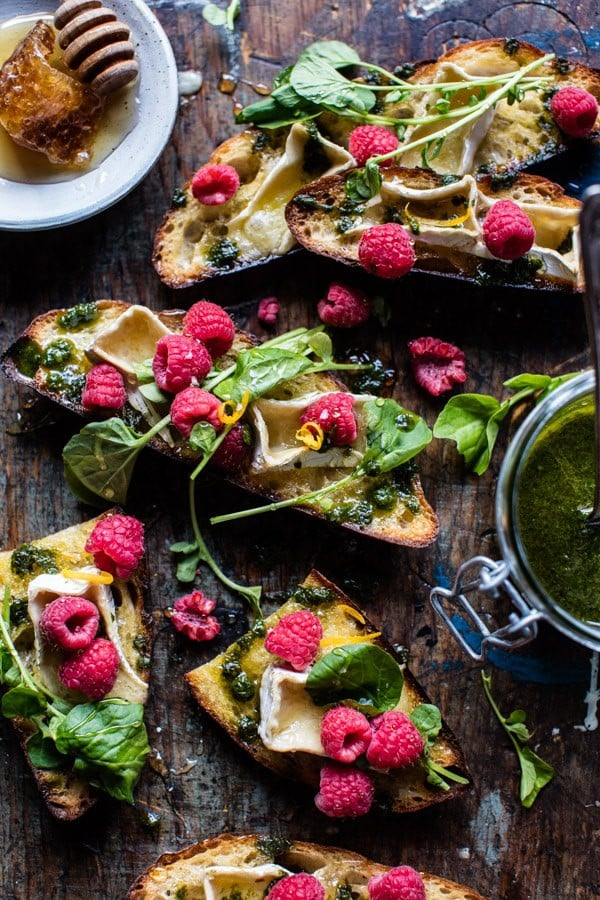
\includegraphics[width=1\textwidth,height=\textheight]{images/honey-raspberry-brie-crostini-with-basil-oil.jpg}

\textbf{Prep Time:} 5 min \textbar{} \textbf{Cook Time:} 10 min
\textbar{} \textbf{Total Time:} 15 min

\section{Ingredients}\label{ingredients-108}

\begin{itemize}
\tightlist
\item
  1 loaf ciabatta bread, or any crusty bread, sliced
\item
  olive oil, for drizzling
\item
  6-8 ounces brie, cut into wedges
\item
  1-2 cups fresh raspberries
\item
  honey, for drizzling
\item
  watercress or arugula, for serving
\item
  1/3 cup olive oil
\item
  3/4 cup fresh basil
\item
  zest and juice of 1 lemon
\item
  kosher salt and pepper
\end{itemize}

\section{Instructions}\label{instructions-108}

\begin{enumerate}
\def\labelenumi{\arabic{enumi}.}
\tightlist
\item
  Preheat your oven to 400 degrees F.
\item
  Place the slices of bread on a baking sheet and drizzle with olive oil
  on both sides. Sprinkle the toast with salt. Transfer to the oven and
  cook 5 minutes and then flip the bread and add the brie to each piece.
  Return to the oven and cook 5 more minutes.
\item
  Transfer the bread to a serving board. Top with raspberries, drizzle
  with honey and basil oil (recipe below). Top with watercress. EAT.
\end{enumerate}

\bookmarksetup{startatroot}

\chapter{Spicy Moroccan Fried Eggs}\label{spicy-moroccan-fried-eggs}

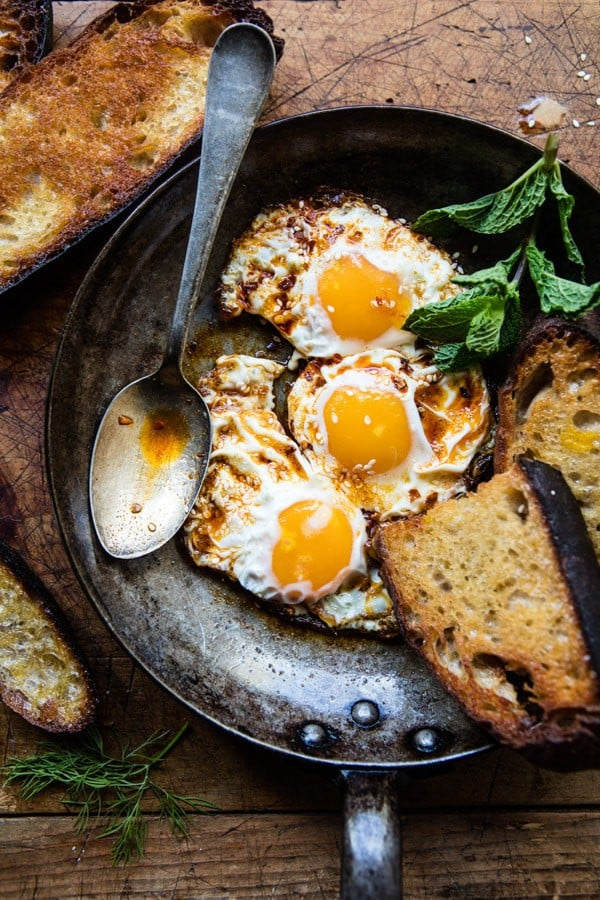
\includegraphics[width=1\textwidth,height=\textheight]{images/spicy-moroccan-fried-eggs.jpg}

\textbf{Prep Time:} 10 min \textbar{} \textbf{Cook Time:} 10 min
\textbar{} \textbf{Total Time:} 20 min

\section{Ingredients}\label{ingredients-109}

\begin{itemize}
\tightlist
\item
  1/4 cup olive oil
\item
  1 teaspoon paprika
\item
  pinch of crushed red pepper flakes
\item
  pinch of saffron
\item
  1 tablespoon olive oil or butter
\item
  6 eggs
\item
  cumin and sesame seeds, for serving
\item
  kosher salt and pepper
\item
  1 cup kalamata olives
\item
  fresh tomatoes, cucumbers, fruit, dried fruit, nuts, and bread, for
  serving
\end{itemize}

\section{Instructions}\label{instructions-109}

\begin{enumerate}
\def\labelenumi{\arabic{enumi}.}
\tightlist
\item
  In a small saucepan, combine the olive oil, paprika, crushed red
  pepper flakes, and saffron over medium heat. Cook 5 minutes to infuse
  the oil and then remove from the heat.
\item
  Heat a skillet with a little olive oil or butter over medium-high heat
  and fry the eggs to your liking. Season with cumin, salt, and pepper.
  Sprinkle with sesame seeds and then drizzle with the infused oil.
  Break the yolk and serve with bread and olives.
\end{enumerate}

\bookmarksetup{startatroot}

\chapter{Pistachio Rose Rice Pudding}\label{pistachio-rose-rice-pudding}

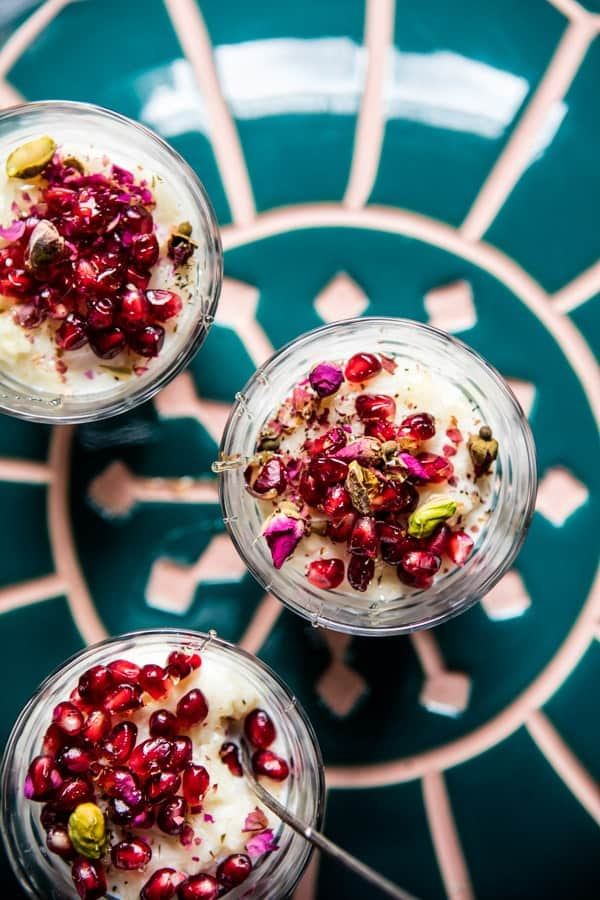
\includegraphics[width=1\textwidth,height=\textheight]{images/pistachio-rose-rice-pudding.jpg}

\textbf{Prep Time:} 10 min \textbar{} \textbf{Cook Time:} 30 min
\textbar{} \textbf{Total Time:} 40 min

\section{Ingredients}\label{ingredients-110}

\begin{itemize}
\tightlist
\item
  4 cups coconut milk, plus more if desired
\item
  1/4 cup honey, plus more for serving
\item
  pinch of salt
\item
  1 cup uncooked rice
\item
  1 teaspoon vanilla extract
\item
  zest from one orange
\item
  1 teaspoon rose water
\item
  1/2 cup toasted unsweetened coconut
\item
  1/2 cup toasted pistachios
\item
  arils from 1 pomegranate
\end{itemize}

\section{Instructions}\label{instructions-110}

\begin{enumerate}
\def\labelenumi{\arabic{enumi}.}
\tightlist
\item
  Combine the coconut milk, honey, and a pinch of salt in a medium
  saucepan and bring to a simmer. Add the rice and stir. Reduce heat to
  low, cover the pot slightly, and cook for about 30 minutes stirring
  every few minutes. If skin starts to form on top of the milk, just
  stir it back in. The milk will reduce and thicken. Once the rice is
  cooked and the milk has thickened add the vanilla, orange zest and
  rose water. Remove from the heat and allow to cool slightly. Ladle
  into jars and chill in the fridge (or eat warm!).
\item
  To serve, sprinkle each serving of pudding with toasted coconut and
  pistachios. Add the pomegranate arils. Enjoy!
\end{enumerate}

\bookmarksetup{startatroot}

\chapter{Moroccan Pancakes (Beghrir).}\label{moroccan-pancakes-beghrir.}

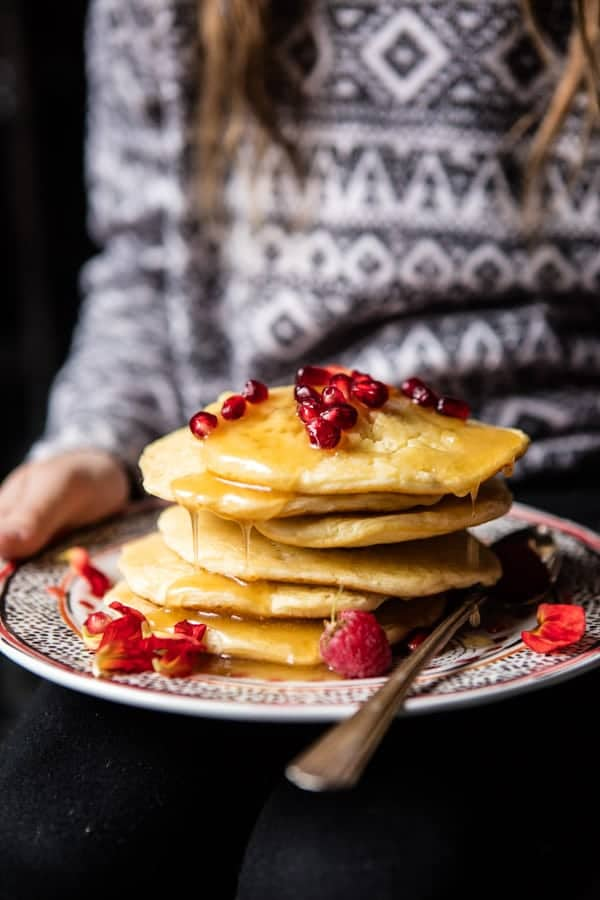
\includegraphics[width=1\textwidth,height=\textheight]{images/moroccan-pancakes-beghrir-.jpg}

\textbf{Prep Time:} 15 min \textbar{} \textbf{Cook Time:} 10 min
\textbar{} \textbf{Total Time:} 25 min

\section{Ingredients}\label{ingredients-111}

\begin{itemize}
\tightlist
\item
  1 cup all purpose flour
\item
  1 cup semolina flour
\item
  2 teaspoons baking powder
\item
  1 1/2 teaspoons instant yeast
\item
  1/2 teaspoon salt
\item
  2 eggs
\item
  1 1/2 cups warm milk
\item
  1/2 cup honey
\item
  4 tablespoons salted butter
\end{itemize}

\section{Instructions}\label{instructions-111}

\begin{enumerate}
\def\labelenumi{\arabic{enumi}.}
\tightlist
\item
  In a medium mixing bowl, combine the flour, semolina flour, baking
  powder, instant yeast, and salt. Add the eggs and milk and mix until
  just combined. Let the better sit 10 minutes or up to overnight,
  covered in the fridge. Bring to room temp before serving.
\item
  Heat a large skillet or griddle over medium heat and lightly grease
  with oil. Pour about 1/4 cup batter onto the center of the hot pan.
  Cook until bubbles appear and the surface is no longer shiny, do not
  flip these. Repeat with the remaining bater.
\item
  In a small saucepan, melt together the honey and butter.
\item
  Serve the pancakes warm, drizzled with honey butter and a side of
  fruit.
\end{enumerate}

\bookmarksetup{startatroot}

\chapter{California Chicken, Avocado and Goat Cheese
Salad}\label{california-chicken-avocado-and-goat-cheese-salad}

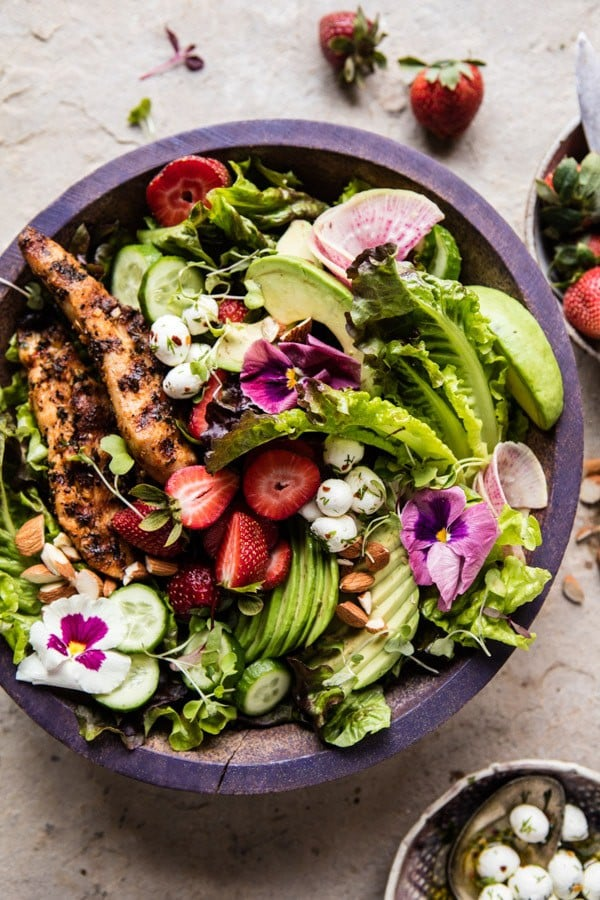
\includegraphics[width=1\textwidth,height=\textheight]{images/california-chicken-avocado-and-goat-cheese-salad.jpg}

\textbf{Prep Time:} 20 min \textbar{} \textbf{Cook Time:} 10 min
\textbar{} \textbf{Total Time:} 30 min

\section{Ingredients}\label{ingredients-112}

\begin{itemize}
\tightlist
\item
  1 pound boneless skinless chicken tenders
\item
  1/4 cup extra virgin olive oil
\item
  4 cloves garlic, minced or grated
\item
  1/4 cup fresh parsley, chopped ((or 1 tablespoon dried))
\item
  1/4 cup fresh basil, chopped ((or 1 tablespoon dried))
\item
  1/2 teaspoon smoked paprika
\item
  1/2 teaspoon onion powder
\item
  1/4 teaspoon cayenne
\item
  1/2 teaspoon kosher salt and pepper
\item
  2 heads romaine lettuce, chopped
\item
  1 cup fresh strawberries, halved
\item
  2 watermelon radishes, thinly slice
\item
  2 Persian cucumbers, sliced
\item
  4 ounces herbed goat cheese, crumbled
\item
  1 avocado, sliced
\item
  1/2 cup roasted almonds, chopped
\item
  large handful micro greens, sprouts, and or edible flowers, for
  serving
\item
  1/4 cup olive oil
\item
  1/4 cup balsamic vinegar
\item
  2 tablespoons apple cider vinegar
\item
  1 tablespoon honey
\item
  pinch of cayenne ((to taste))
\item
  kosher salt and pepper
\end{itemize}

\section{Instructions}\label{instructions-112}

\begin{enumerate}
\def\labelenumi{\arabic{enumi}.}
\tightlist
\item
  In a bowl, combine the chicken, olive oil, garlic, parsley, basil,
  paprika, onion powder, cayenne, salt, and pepper. For added flavor,
  allow the chicken to marinate 1 hour or overnight.
\item
  Preheat your grill, grill pan or cast iron skillet to medium high and
  brush the grates with oil.
\item
  Grill the chicken for 5-8 minutes per side or until the chicken is
  cooked through. Remove from the grill and thinly slice the chicken.
\item
  In a large salad bowl, toss together the lettuce, strawberries,
  radishes, and cucumbers. Add the chicken on top of the salad along
  with the goat cheese, avocado, almonds, and a handful of micro greens.
  Serve with the honey balsamic (below).
\end{enumerate}

\bookmarksetup{startatroot}

\chapter{Island Mango Mezcal Breeze}\label{island-mango-mezcal-breeze}

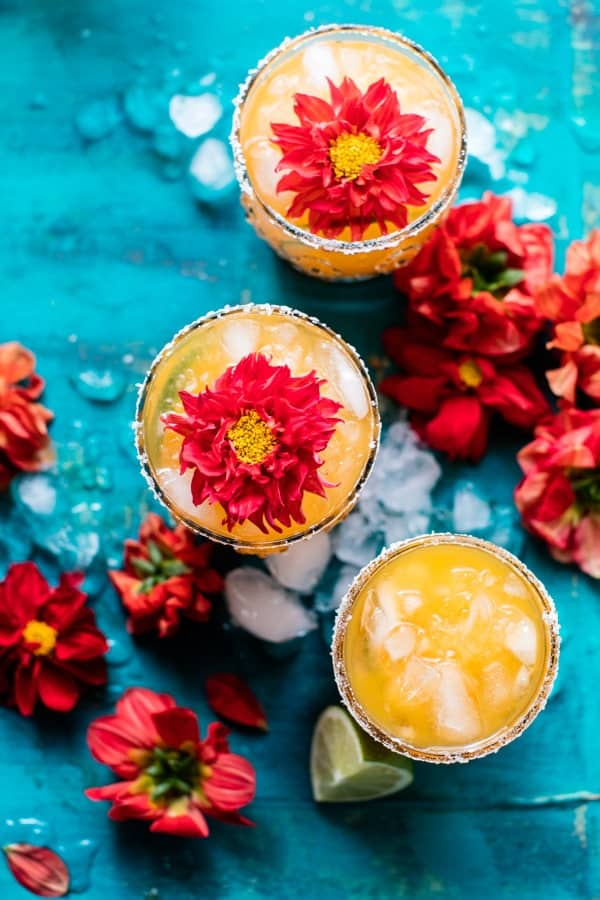
\includegraphics[width=1\textwidth,height=\textheight]{images/island-mango-mezcal-breeze.jpg}

\textbf{Prep Time:} 5 min \textbar{} \textbf{Cook Time:} \textbar{}
\textbf{Total Time:} 5 min

\section{Ingredients}\label{ingredients-113}

\begin{itemize}
\tightlist
\item
  salt, for the rim
\item
  1/4 cup mango juice
\item
  juice of 1/2 a lemon
\item
  juice of 1/2 a lime
\item
  1 1/2 ounces Mezcal
\item
  1 1/2 ounces silver tequila
\item
  pinch of chili powder, to taste
\item
  sparkling water for topping
\end{itemize}

\section{Instructions}\label{instructions-113}

\begin{enumerate}
\def\labelenumi{\arabic{enumi}.}
\tightlist
\item
  Run a lime wedge around the rim of your glass and coat in salt.
\item
  Combine the mango juice, lemon juice, lime juice, Mezcal, tequila, and
  chili powder in a cocktail shaker and fill with ice. Shake until
  combined and then strain into your prepared glass. Top with sparkling
  water. Serve with limes. Drink!
\end{enumerate}

\bookmarksetup{startatroot}

\chapter{Peanut Butter Swirled Chocolate Fudge
Popsicles}\label{peanut-butter-swirled-chocolate-fudge-popsicles}

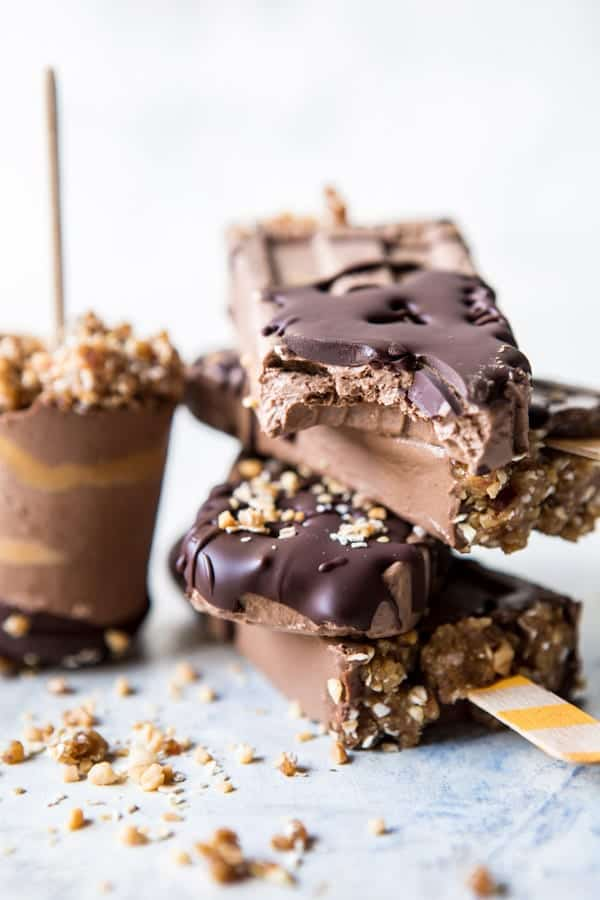
\includegraphics[width=1\textwidth,height=\textheight]{images/peanut-butter-swirled-chocolate-fudge-popsicles.jpg}

\textbf{Prep Time:} 15 min \textbar{} \textbf{Cook Time:} \textbar{}
\textbf{Total Time:} 15 min

\section{Ingredients}\label{ingredients-114}

\begin{itemize}
\tightlist
\item
  1 (14 ounce) can full fat canned coconut milk
\item
  1/4 + 1/3 cup creamy peanut butter
\item
  2 ripe bananas
\item
  6-8 dates + 1/3 cup pitted medjool dates
\item
  1/2 cup cacao or cocoa powder
\item
  3 tablespoons hemp seeds
\item
  2 teaspoons vanilla extract
\item
  1/2 cup rolled oats
\item
  1/2 cup roasted peanuts
\item
  8 ounces dark chocolate, melted
\end{itemize}

\section{Instructions}\label{instructions-114}

\begin{enumerate}
\def\labelenumi{\arabic{enumi}.}
\tightlist
\item
  In a high powder blender or food processor, combine the coconut milk,
  1/4 cup peanut butter, bananas, 6-8 dates, cacao powder, hemp seeds,
  and vanilla and blend until completely smooth and the consistency of a
  thick smoothie.
\item
  To assemble, layer the chocolate mix and the remaining 1/3 cup peanut
  butter evenly among 10-12 popsicles molds. It's OK if the layers are
  not perfect.
\item
  To make the granola: in a food processor, combine the remaining 1/3
  cup dates, oats, and peanuts and pulse until the mix is finely ground
  and resembles granola. Sprinkle the ``granola'' over the tops of the
  pops, gently pressing into the pops (you will not use all the
  ``granola''). Insert popsicle sticks, cover the tops of the mold and
  freeze until firm, about 4 hours. To remove the popsicles run the mold
  under hot water for 10 seconds and then pull the popsicles out of the
  molds.
\item
  If desired, dip each popsicle in chocolate and then quickly sprinkle
  with the remaining ``granola''. Store in the freezer.
\end{enumerate}

\bookmarksetup{startatroot}

\chapter{Breakfast Tacos Al Pastor}\label{breakfast-tacos-al-pastor}

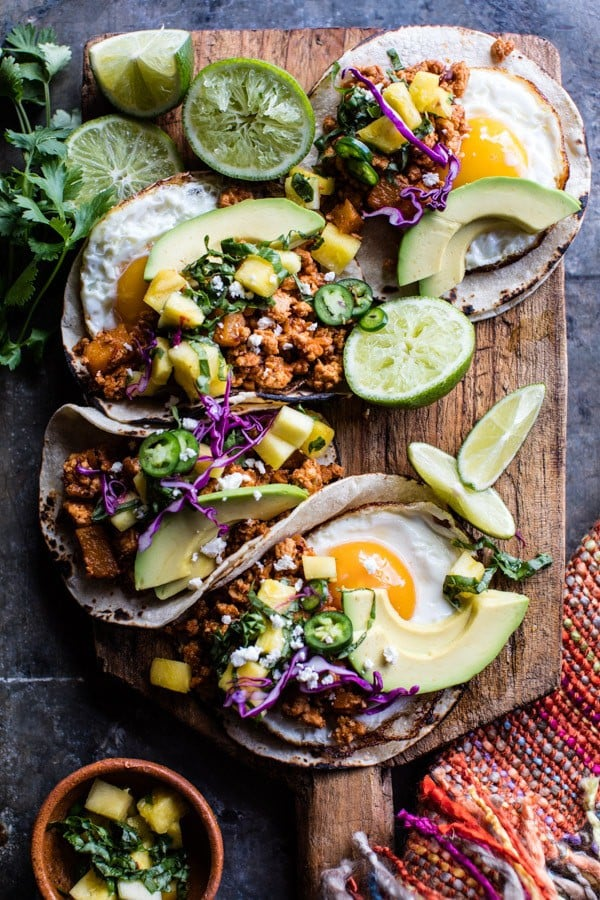
\includegraphics[width=1\textwidth,height=\textheight]{images/breakfast-tacos-al-pastor.jpg}

\textbf{Prep Time:} 10 min \textbar{} \textbf{Cook Time:} 20 min
\textbar{} \textbf{Total Time:} 30 min

\section{Ingredients}\label{ingredients-115}

\begin{itemize}
\tightlist
\item
  2 tablespoons olive oil
\item
  1 pound ground chicken or pork
\item
  1/2 sweet onion, chopped
\item
  2 cloves garlic, minced or grated
\item
  2 teaspoons chili powder
\item
  1 teaspoon paprika
\item
  1 teaspoon kosher salt
\item
  2 chipotle peppers in adobo, chopped
\item
  1/2 cup not-from-concentrate Florida's Natural® Brand Orange Juice
\item
  2 cups fresh pineapple chunks
\item
  1/4 cup fresh cilantro, chopped
\item
  1/4 cup fresh basil, chopped
\item
  1 jalapeño, seeded and chopped
\item
  juice of 1 lime
\item
  6-8 corn or flour tortillas, warmed
\item
  4-6 fried eggs
\item
  sliced avocado, for serving
\item
  feta or cheddar cheese, for serving
\end{itemize}

\section{Instructions}\label{instructions-115}

\begin{enumerate}
\def\labelenumi{\arabic{enumi}.}
\tightlist
\item
  In a large skillet, heat the olive oil over high heat. When the oil
  shimmers, add the ground chicken and onion. Cook, stirring often and
  breaking up the meat as it cooks, until the chicken is browned, about
  5 minutes. Add the garlic, chili powder, paprika, salt, chipotle
  peppers, Florida’s Natural orange juice, 1/4 cup water, and 1 cup
  pineapple. Reduce the heat to medium and simmer until the sauce has
  thickened slightly around the chicken, about 10-15 minutes. Remove
  from the heat and stir in the cilantro.
\item
  Meanwhile, in a bowl, combine the remaining 1 cup pineapple, the
  basil, jalapeño, lime juice, and a pinch of salt.
\item
  To serve, divide the fried eggs among tortillas and top with the
  chicken. Add the pineapple-basil-salsa, avocado, and cheese. EAT!
\end{enumerate}

\bookmarksetup{startatroot}

\chapter{Greek Lemon Garlic Roasted Broccoli Pasta
Salad}\label{greek-lemon-garlic-roasted-broccoli-pasta-salad}

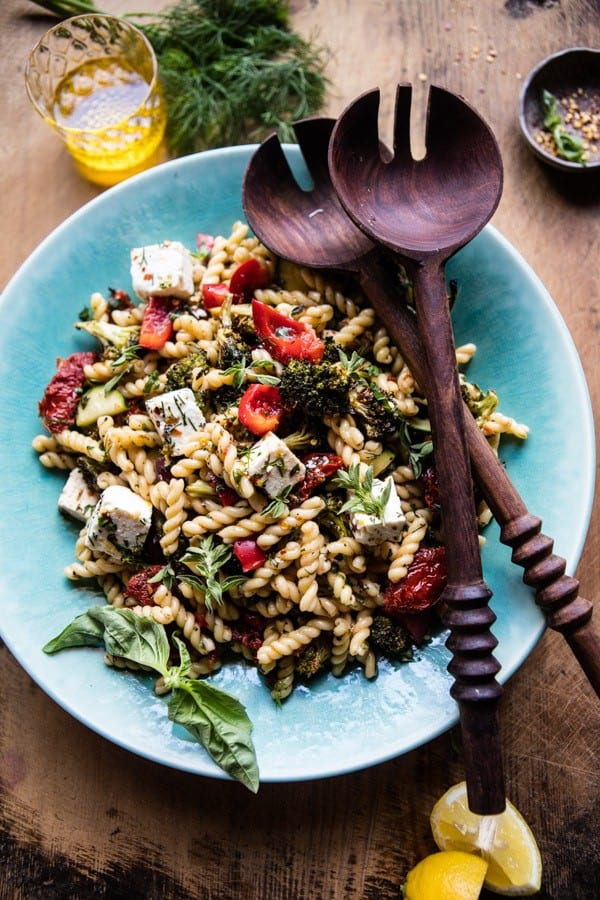
\includegraphics[width=1\textwidth,height=\textheight]{images/greek-lemon-garlic-roasted-broccoli-pasta-salad.jpg}

\textbf{Prep Time:} 10 min \textbar{} \textbf{Cook Time:} 20 min
\textbar{} \textbf{Total Time:} 30 min

\section{Ingredients}\label{ingredients-116}

\begin{itemize}
\tightlist
\item
  2 heads broccoli, florets roughly chopped
\item
  1/3 cup pine nuts
\item
  2 tablespoons olive oil
\item
  2-4 cloves garlic, minced or grated
\item
  kosher salt and pepper
\item
  1 pound short cut pasta
\item
  1 (8 ounce) jar oil packed sun-dried tomatoes
\item
  1/2 cup pitted kalamata olives
\item
  1 zucchini thinly, sliced
\item
  1 red bell pepper, sliced
\item
  2 Persian cucumbers, chopped
\item
  1/4 cup fresh oregano, chopped
\item
  1/4 cup fresh basil, chopped
\item
  2 tablespoons chopped fresh dill
\item
  juice and zest of 1 lemon
\item
  8 ounces feta cheese, cubed
\end{itemize}

\section{Instructions}\label{instructions-116}

\begin{enumerate}
\def\labelenumi{\arabic{enumi}.}
\tightlist
\item
  Preheat the oven to 425 degrees F.
\item
  On a large baking sheet, toss together the broccoli, pine nuts, 2
  tablespoons olive oil, garlic, and a large pinch of both salt and
  pepper. Transfer to the oven and roast for 20-25 minutes or until the
  broccoli is just beginning to char.
\item
  Meanwhile, bring a large pot of salted water to a boil over high heat.
  Cook the pasta according to package directions until al dente. Drain
  and add back to the hot pot.
\item
  While the pasta is still warm, add the roasted broccoli, sun-dried
  tomatoes - plus the oil in the jar, olives and 3 tablespoons of the
  olive brine (the liquid surrounding the olives), the zucchini, red
  pepper, cucumbers, oregano, basil, dill, lemon juice and zest. Toss
  until well combined and the pasta is coated in oil, if needed drizzle
  in little olive oil over if there doesn't seem to be enough. Add the
  feta and gently toss. Serve warm or at room temperature. The pasta can
  be made up to 1 day in advance.
\end{enumerate}

\bookmarksetup{startatroot}

\chapter{Cauliflower Rice Carne Asada Bowls with Mango
Salsa}\label{cauliflower-rice-carne-asada-bowls-with-mango-salsa}

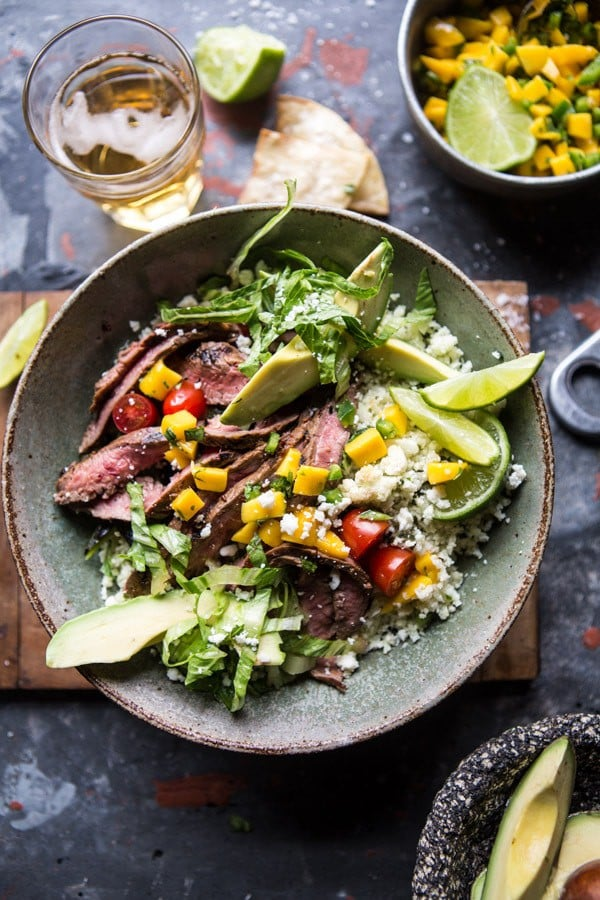
\includegraphics[width=1\textwidth,height=\textheight]{images/cauliflower-rice-carne-asada-bowls-with-mango-salsa.jpg}

\textbf{Prep Time:} 15 min \textbar{} \textbf{Cook Time:} 15 min
\textbar{} \textbf{Total Time:} 1 hr

\section{Ingredients}\label{ingredients-117}

\begin{itemize}
\tightlist
\item
  1 1/2 pounds flank steak
\item
  1/4 cup olive oil
\item
  1/3 cup orange juice
\item
  4 cloves garlic, minced or grated
\item
  1 chipotle pepper in adobo, chopped ((or 2 teaspoons chili powder))
\item
  zest and juice of 1 lime
\item
  1/2 cup fresh cilantro, chopped
\item
  shredded lettuce, sliced avocado, and cheese, for serving
\item
  2 cups riced cauliflower ((about 1 large head pulsed in a food
  processor))
\item
  1 tablespoon olive oil
\item
  1 teaspoon cumin
\item
  1/4 cup fresh cilantro chopped
\item
  1 mango, chopped
\item
  1 jalapeño, seeded and chopped
\item
  juice of 1 lime
\item
  1/4 cup fresh cilantro, chopped
\end{itemize}

\section{Instructions}\label{instructions-117}

\begin{enumerate}
\def\labelenumi{\arabic{enumi}.}
\tightlist
\item
  Add the steak to a ziplock bag and add the olive oil, orange juice,
  garlic, chipotle peppers, lime zest and juice, and the cilantro. Seal
  the bag and marinate 30 minutes or in the fridge as long as overnight.
\item
  Meanwhile, make the cauliflower rice. Preheat the oven to 425 degrees
  F.
\item
  Spread the riced cauliflower out on a large baking sheet and toss
  together with the olive oil, cumin, and a large pinch of salt.
  Transfer to the oven and cook 10 minutes, toss and cook 10 minutes
  more or until the cauliflower is tender. Remove and stir in the
  cilantro and juice + zest of 1/2 a lime juice.
\item
  Preheat your grill or grill pan to high.
\item
  Remove the steak from its marinade and sear the steak for 5-8 minutes,
  flip and sear another 5 minutes or until your desired doneness is
  reached. Remove the steak from the grill and allow to rest 10 minutes.
  Slice steak thinly against the grain.
\item
  To make the salsa. In a bowl, combine the mango, jalapeño, lime
  juice, cilantro, and a pinch of salt.
\item
  To serve, divide the rice among bowls and top with steak, lettuce,
  avocado, salsa, and cheese, EAT!
\end{enumerate}

\bookmarksetup{startatroot}

\chapter{Cuban Grilled Salmon with Tomato Avocado
Salsa}\label{cuban-grilled-salmon-with-tomato-avocado-salsa}

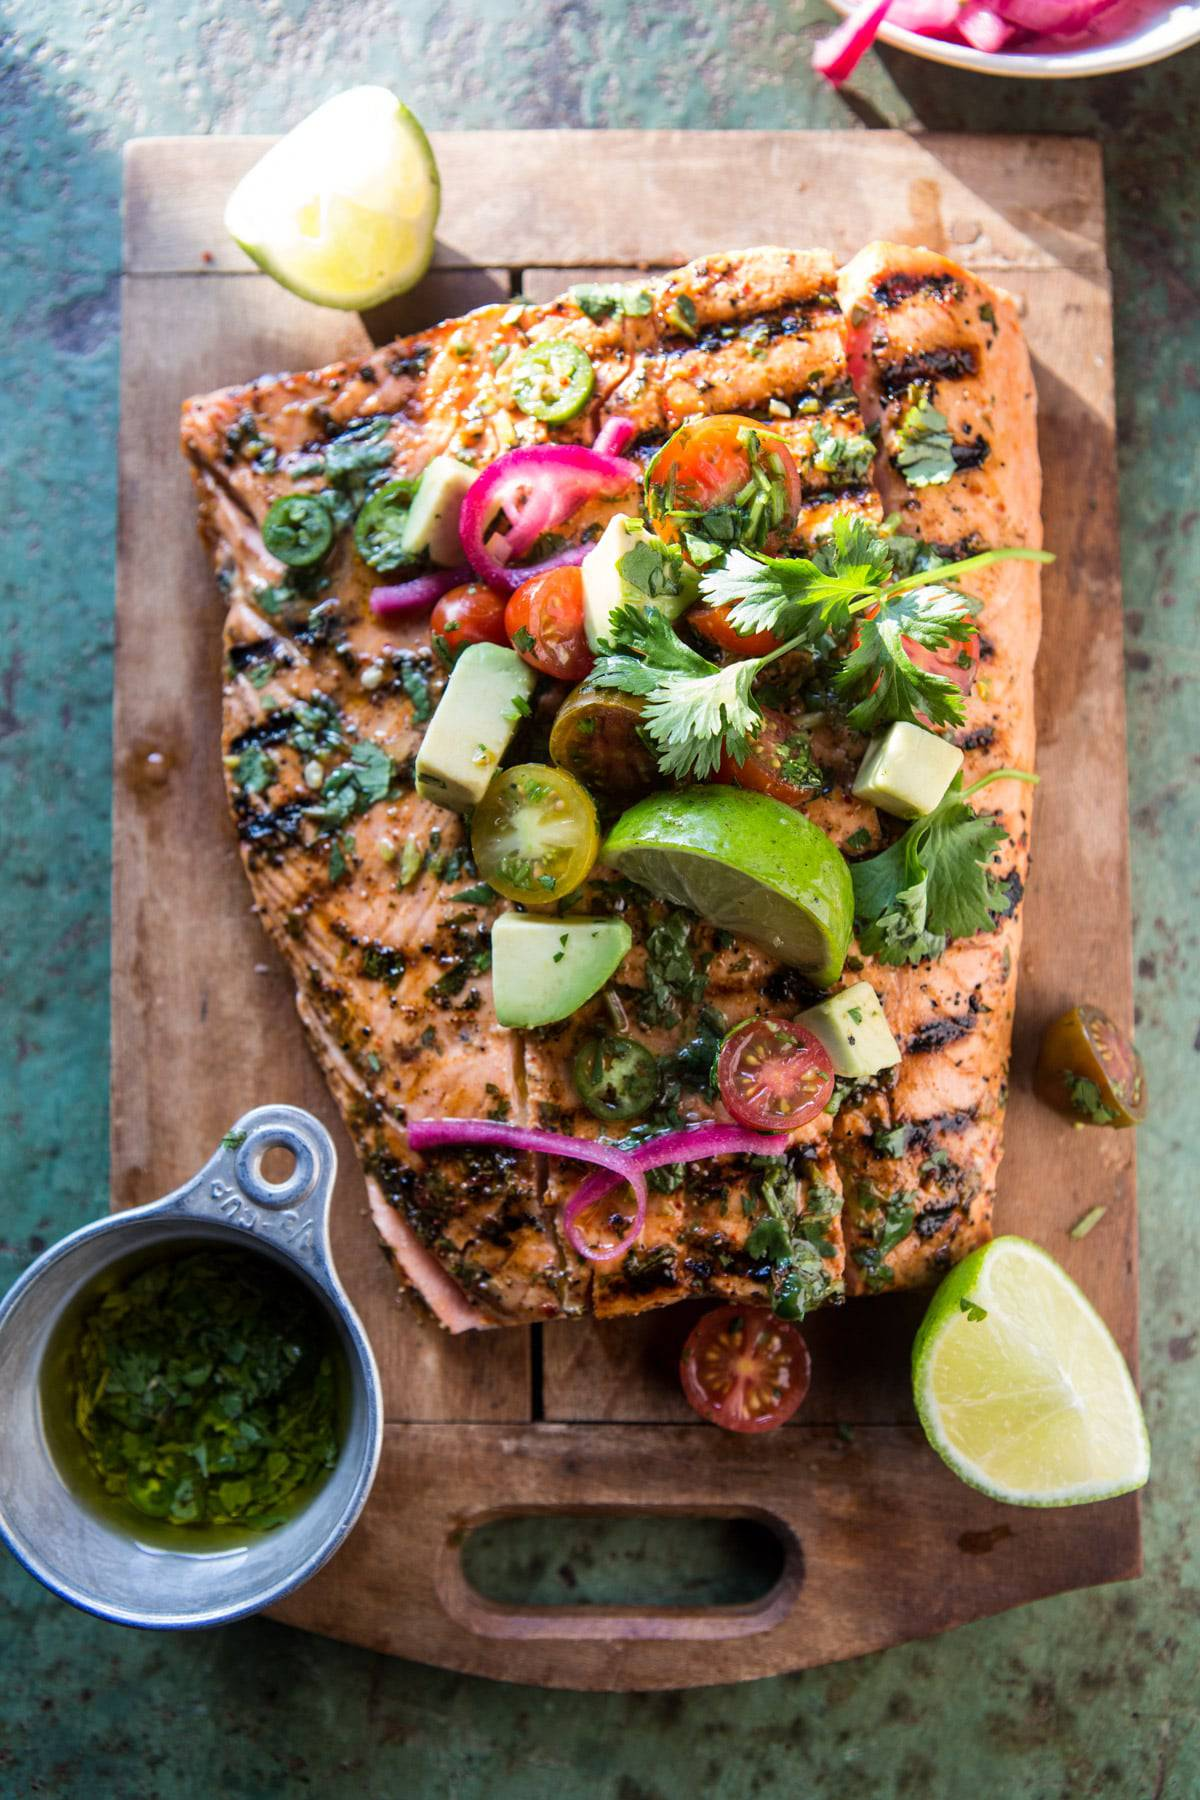
\includegraphics[width=1\textwidth,height=\textheight]{images/cuban-grilled-salmon-with-tomato-avocado-salsa.jpg}

\textbf{Prep Time:} 15 min \textbar{} \textbf{Cook Time:} 10 min
\textbar{} \textbf{Total Time:} 25 min

\section{Ingredients}\label{ingredients-118}

\begin{itemize}
\tightlist
\item
  1 pound wild caught salmon
\item
  1/4 cup olive oil
\item
  juice of 1 lime
\item
  1/4 cup freshly squeezed orange juice
\item
  3 cloves garlic
\item
  2 green onions
\item
  1 teaspoon cumin
\item
  1 teaspoon cayenne pepper
\item
  1 teaspoon kosher salt and pepper
\item
  1 tablespoon salted butter
\item
  2 cups cherry tomatoes, halved
\item
  2 ripe avocados, diced
\item
  juice of 1 lime
\item
  1/4 cup fresh cilantro, chopped
\item
  1 jalapeño pepper, seeded and diced
\item
  pinch of sea salt
\end{itemize}

\section{Instructions}\label{instructions-118}

\begin{enumerate}
\def\labelenumi{\arabic{enumi}.}
\tightlist
\item
  Place the salmon in a 9x13 inch baking dish.
\item
  In a blender, combine the olive oil, lime juice, orange juice, garlic,
  green onions, cumin, cayenne, salt and pepper. Pulse until combined.
  Pour the marinade over the salmon and let set for 15 minutes.
\item
  Heat your grill, grill pan or skillet to medium high heat.
\item
  Transfer the salmon to the preheated grill and grill for about 3
  minutes on each side or until the salmon is cooked to your desired
  doneness, brush the salmon with the marinade as it cooks. Remove the
  salmon from the grill.
\item
  To serve, pat the salmon with butter and allow it to melt. Serve
  topped with the tomato avocado salsa. Enjoy!
\end{enumerate}

\bookmarksetup{startatroot}

\chapter{Strawberry Ripple Almond
Cheesecake}\label{strawberry-ripple-almond-cheesecake}

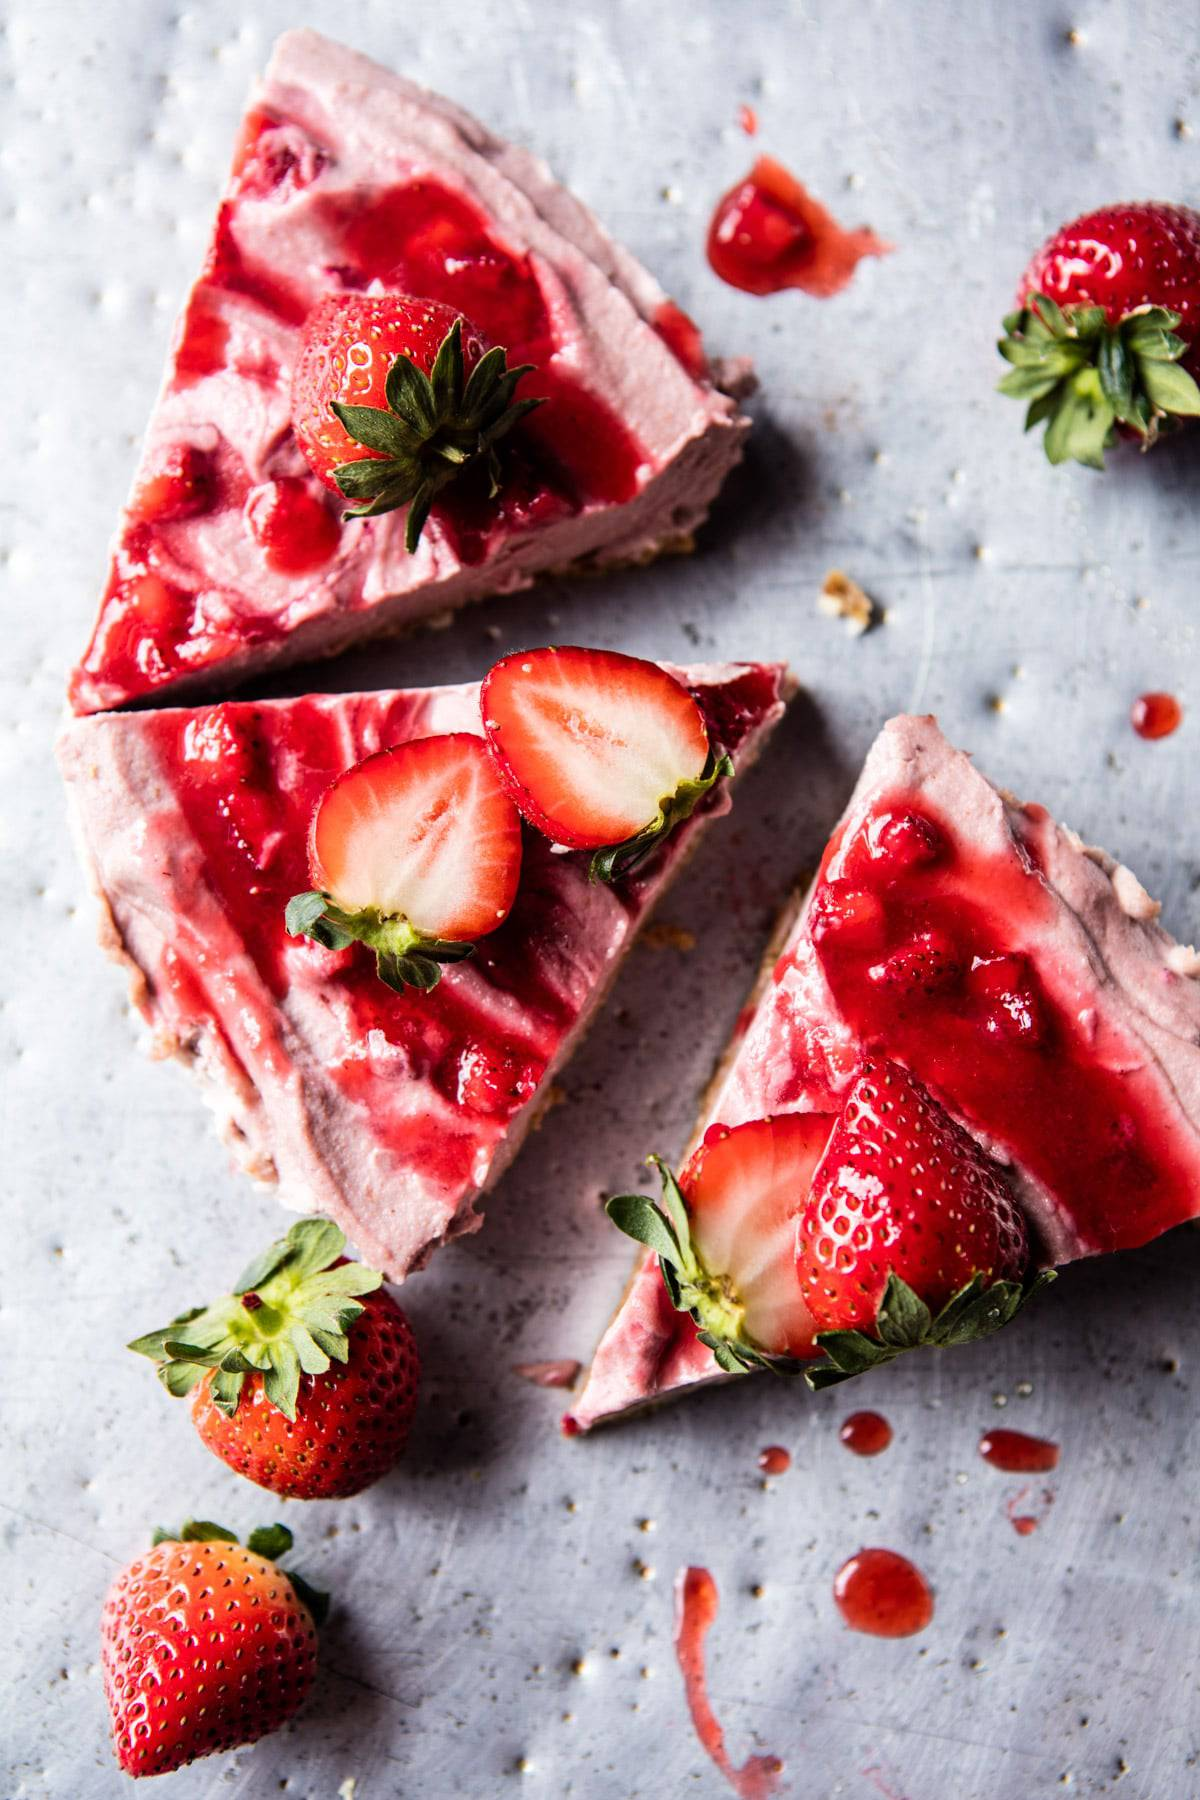
\includegraphics[width=1\textwidth,height=\textheight]{images/strawberry-ripple-almond-cheesecake.jpg}

\textbf{Prep Time:} 15 min \textbar{} \textbf{Cook Time:} 10 min
\textbar{} \textbf{Total Time:} 25 min

\section{Ingredients}\label{ingredients-119}

\begin{itemize}
\tightlist
\item
  1/2 cup raw almonds
\item
  1/2 cup unsweetened coconut
\item
  1/4 cup old fashioned oats
\item
  1 cup packed dates, pitted
\item
  pinch of flaky sea salt
\item
  4 1/2 cups roughly chopped strawberries
\item
  1/2 cup honey ((agave or maple if vegan))
\item
  juice of 1 lemon
\item
  2 cups raw blanched almonds, soaked overnight in water
\item
  1 cup Almond Breeze Unsweetened Original Almondmilk
\item
  1/2 cup coconut oil
\item
  1 teaspoon vanilla extract
\item
  fresh strawberries for serving
\end{itemize}

\section{Instructions}\label{instructions-119}

\begin{enumerate}
\def\labelenumi{\arabic{enumi}.}
\tightlist
\item
  To make the crust. In the bowl of a food processor, combine the raw
  almonds, coconut, oats, dates, and pinch of salt. Pulse until finely
  chopped and easily holds together when squeezed in your hand. Press
  the base mixture into a 8-inch spring form pan. Place the pan in the
  freezer.
\item
  To make the filling. In a medium pot, bring the strawberries, honey,
  and lemon juice to a boil. Boil 8-10 minutes or until the mixture has
  thickened and becomes jam-like. Stir in a pinch of salt. Let cool and
  then puree in a blender.
\item
  Drain the almonds and add them to the bowl of your food processor with
  the Almondmilk, coconut oil, and vanilla. Pulse until smooth and
  creamy. Add 3/4 of the strawberry puree and pulse until combined.
  Remove the base layer from the freezer and add the almond cream in an
  even layer. Using a knife, swirl in the remaining strawberry puree.
  Cover and place in the freezer until firm, 1-2 hours. Remove 10
  minutes before serving.
\end{enumerate}

\bookmarksetup{startatroot}

\chapter{Cheesy Chipotle Adobo Chicken
Quesadillas}\label{cheesy-chipotle-adobo-chicken-quesadillas}


\includegraphics[width=1\textwidth,height=\textheight]{images/cheesy-chipotle-adobo-chicken-quesadillas.jpg}

\textbf{Prep Time:} 15 min \textbar{} \textbf{Cook Time:} 30 min
\textbar{} \textbf{Total Time:} 45 min

\section{Ingredients}\label{ingredients-120}

\begin{itemize}
\tightlist
\item
  2 tablespoons olive oil
\item
  1 pound boneless skinless chicken tenders or small breasts
\item
  1 poblano pepper, sliced
\item
  1 (14 ounce) can fire roasted diced tomatoes
\item
  2 chipotle peppers in adobo, chopped
\item
  1 teaspoon chili powder
\item
  1 teaspoon dried oregano
\item
  1 teaspoon cumin
\item
  1 teaspoon kosher salt and pepper
\item
  1/4 cup fresh cilantro, chopped
\item
  8 small corn or flour tortillas
\item
  1 cup white or brown rice
\item
  1 cup shredded cheddar cheese
\item
  1 cup plain Greek yogurt
\item
  zest of 1 lime
\item
  diced mango, pickled red onion, jalapeños, cilantro, and limes, for
  serving
\end{itemize}

\section{Instructions}\label{instructions-120}

\begin{enumerate}
\def\labelenumi{\arabic{enumi}.}
\tightlist
\item
  Heat 1 tablespoon olive oil in a medium size pot over high heat. When
  the oil shimmers, add the chicken and season with salt and pepper.
  Cook until seared on both sides, about 3 minutes per side. Add the
  poblano pepper and cook 3-4 minutes or until just charred.
\item
  Reduce the heat to medium. Add the tomatoes, 1/2 cup water, the
  chipotle peppers, chili powder, oregano, cumin, salt and pepper. Stir
  to combine and then simmer 15-20 minutes, or until the chicken is
  cooked through and shreds easily. Shred the chicken in the pot. Remove
  from the heat and stir in the cilantro.
\item
  Preheat the oven to 450 degrees F.
\item
  On a baking sheet, rub the tortillas with the remaining 1 tablespoon
  olive oil. Lay 4 tortillas flat and then layer evenly with cheese,
  rice, and chicken. Add the top tortilla. Transfer to the oven and cook
  for 5-8 minutes, then flip and cook another 5 minutes more, or until
  the cheese has melted and the tortillas are crisp.
\item
  Meanwhile stir together the yogurt and lime zest. Season to taste with
  salt.
\item
  Serve the quesadillas topped with diced mango, jalapeños, fresh
  cilantro, and drizzled with yogurt. EAT!
\end{enumerate}

\bookmarksetup{startatroot}

\chapter{Easy Lemon Ricotta Old Fashioned
Doughnuts}\label{easy-lemon-ricotta-old-fashioned-doughnuts}

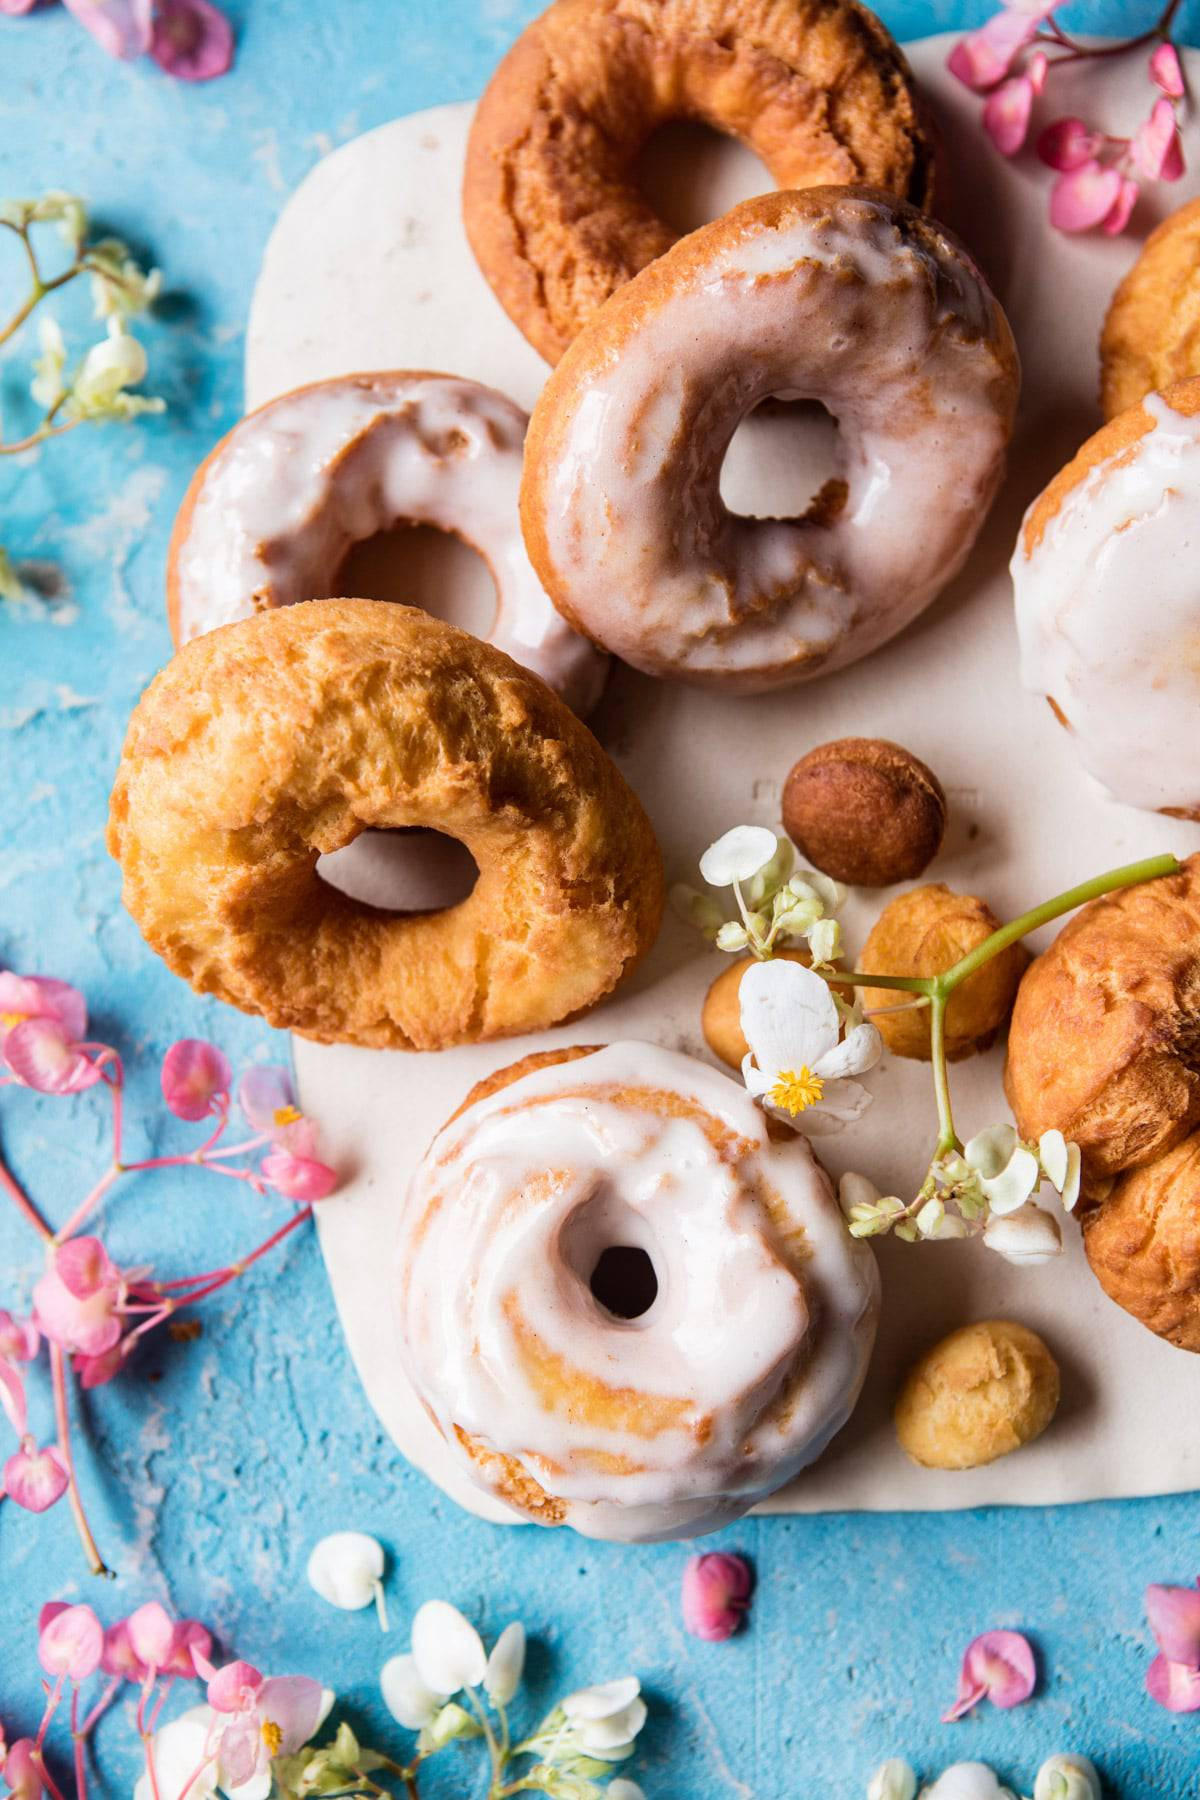
\includegraphics[width=1\textwidth,height=\textheight]{images/easy-lemon-ricotta-old-fashioned-doughnuts.jpg}

\textbf{Prep Time:} 20 min \textbar{} \textbf{Cook Time:} 10 min
\textbar{} \textbf{Total Time:} 30 min

\section{Ingredients}\label{ingredients-121}

\begin{itemize}
\tightlist
\item
  2 eggs
\item
  3/4 cup whole milk ricotta cheese
\item
  2 teaspoons pure vanilla extract
\item
  2 tablespoons unsalted butter, melted
\item
  2 1/2 cups all-purpose flour
\item
  1 tablespoon baking powder
\item
  2 tablespoons granulated sugar
\item
  1 teaspoon salt
\item
  zest of 1 Meyer lemon
\item
  2 cups powdered sugar
\item
  juice of 2 Meyer lemons
\item
  1/4 cup mascarpone cheese at room temperature
\item
  1 teaspoon pure vanilla extract
\end{itemize}

\section{Instructions}\label{instructions-121}

\begin{enumerate}
\def\labelenumi{\arabic{enumi}.}
\tightlist
\item
  In a medium mixing bowl, beat together the eggs, ricotta, vanilla, and
  butter until smooth. Add the flour, baking powder, sugar, salt, and
  lemon zest and beat until just combined. Cover and let sit 10-15
  minutes.
\item
  Heat 2 inches of oil to 350 degrees F.
\item
  Lightly flour a work surface and roll out the dough to a 1/2-inch
  thickness. Using doughnut or cookie cutters, cut out round of dough.
\item
  Working in batches, use a slotted metal spoon or spatula to carefully
  place the doughnuts in the hot oil. Fry, flipping once, until light
  golden brown and puffed, 1 to 2 minutes per side. Drain on a paper
  towel lined plate.
\item
  To make the Glaze. In a medium bowl, beat together the powdered sugar,
  lemon juice, mascarpone, and vanilla until smooth and combined. If
  needed, thin the glaze by adding water, 1 tablespoon at a time, until
  desired consistency is reached.
\item
  Invert the doughnut into the glaze. Allow to set 5 minutes or so.
  Enjoy! These are best eaten the day of making, but taste great the
  next day too!
\end{enumerate}

\bookmarksetup{startatroot}

\chapter{Sun-Dried Tomato Muhammara (Roasted Red Pepper
Spread)}\label{sun-dried-tomato-muhammara-roasted-red-pepper-spread}

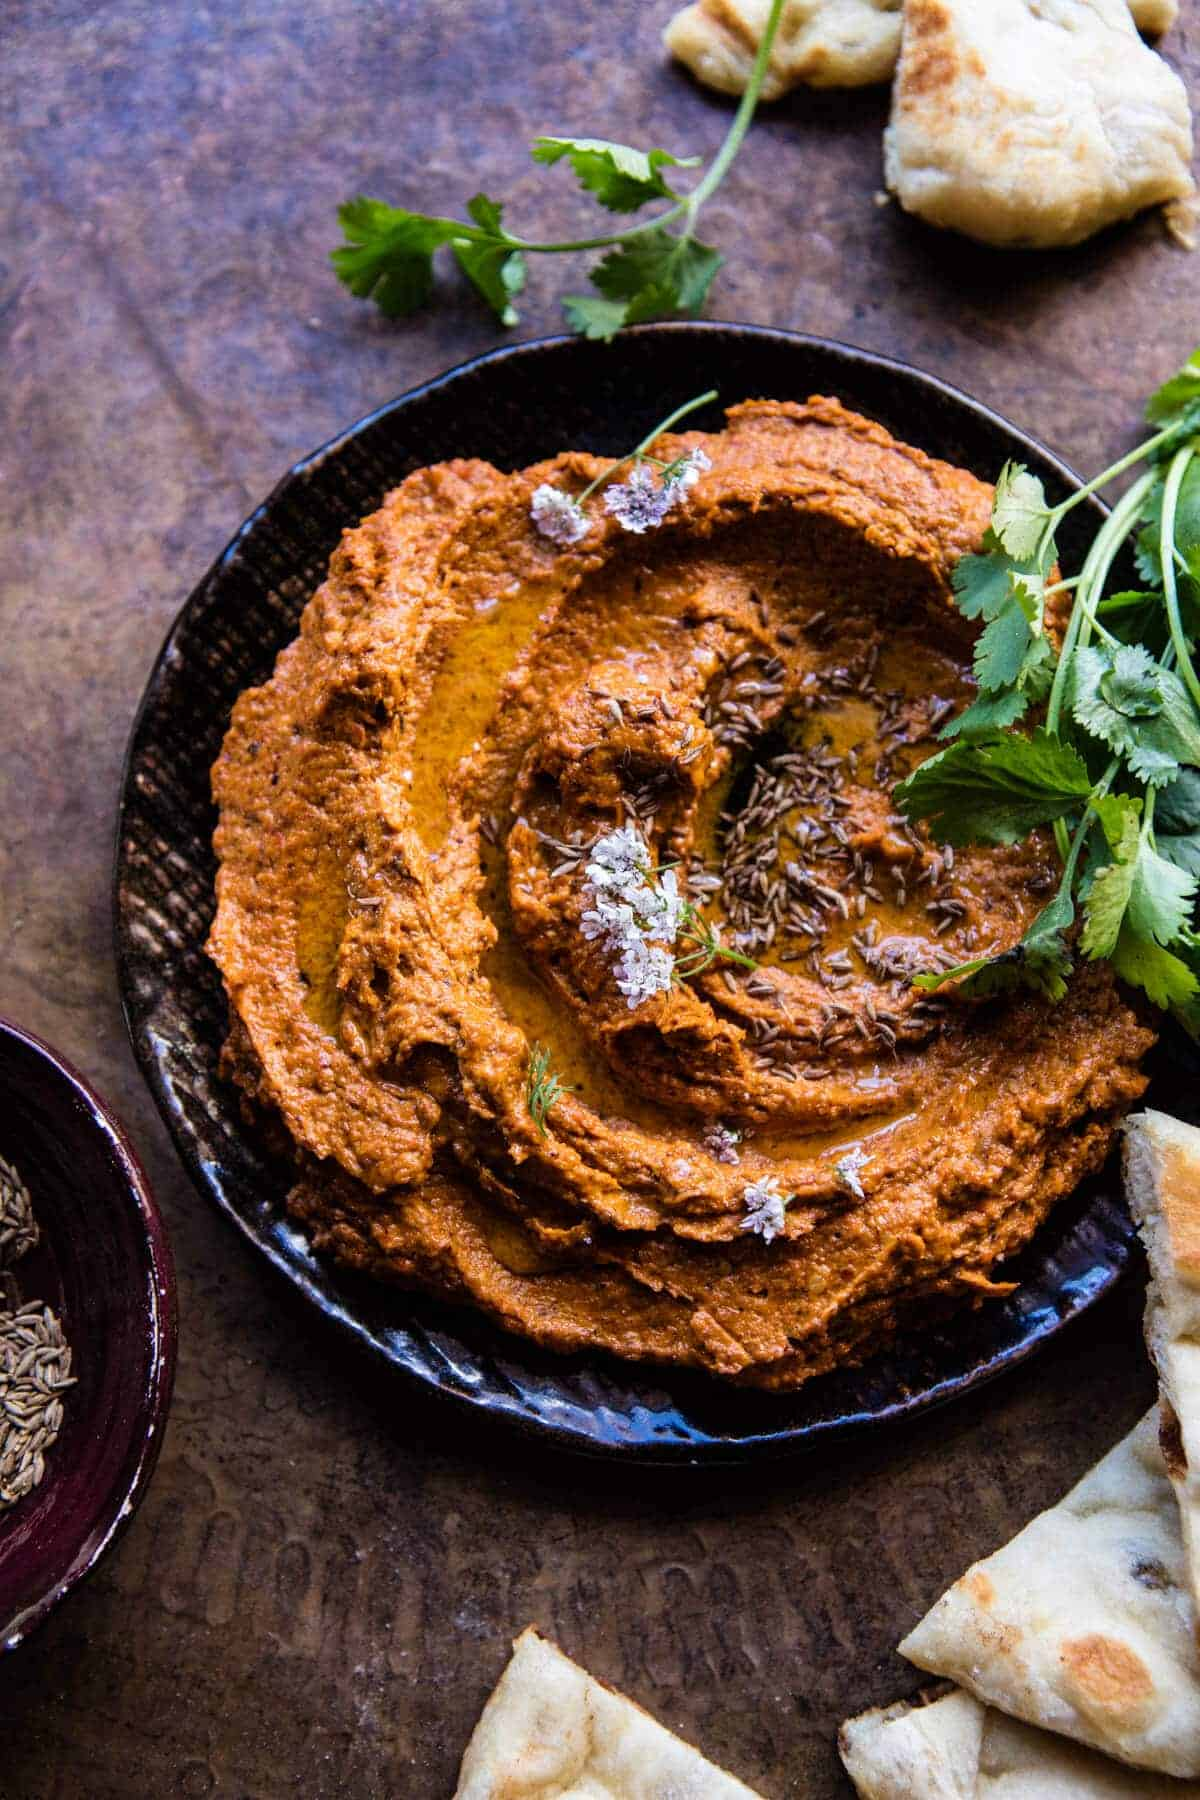
\includegraphics[width=1\textwidth,height=\textheight]{images/sun-dried-tomato-muhammara-roasted-red-pepper-spread-.jpg}

\textbf{Prep Time:} 15 min \textbar{} \textbf{Cook Time:} \textbar{}
\textbf{Total Time:} 15 min

\section{Ingredients}\label{ingredients-122}

\begin{itemize}
\tightlist
\item
  2 roasted red peppers
\item
  1/3 cup sun-dried tomatoes, oil drained
\item
  1/4 cup olive oil (I use the oil from the sun-dried tomatoes)
\item
  juice of 2 lemons
\item
  1 clove garlic, minced or grated
\item
  1/2 teaspoon cumin
\item
  1/2 teaspoon paprika
\item
  1 1/3 cups toasted walnuts, roughly chopped
\item
  kosher salt and pepper
\item
  1 teaspoon cumin seeds
\item
  flakey sea salt
\end{itemize}

\section{Instructions}\label{instructions-122}

\begin{enumerate}
\def\labelenumi{\arabic{enumi}.}
\tightlist
\item
  In a food processor, combine the roasted red peppers, sun-dried
  tomatoes, olive oil, lemon juice, garlic, cumin, paprika, half the
  walnuts and a large pinch of both salt and pepper. Pulse until
  completely smooth and combined. Stir in the remaining walnuts. Heat a
  small skillet over medium heat and add the cumin seeds. cook stirring
  often until toasted, about 3-5 minutes. Spread the dip on a plate and
  drizzle with olive oil. Top with cumin seeds and salt.
\end{enumerate}

\bookmarksetup{startatroot}

\chapter{Blueberry Lemon Poppy Seed
Scones}\label{blueberry-lemon-poppy-seed-scones}

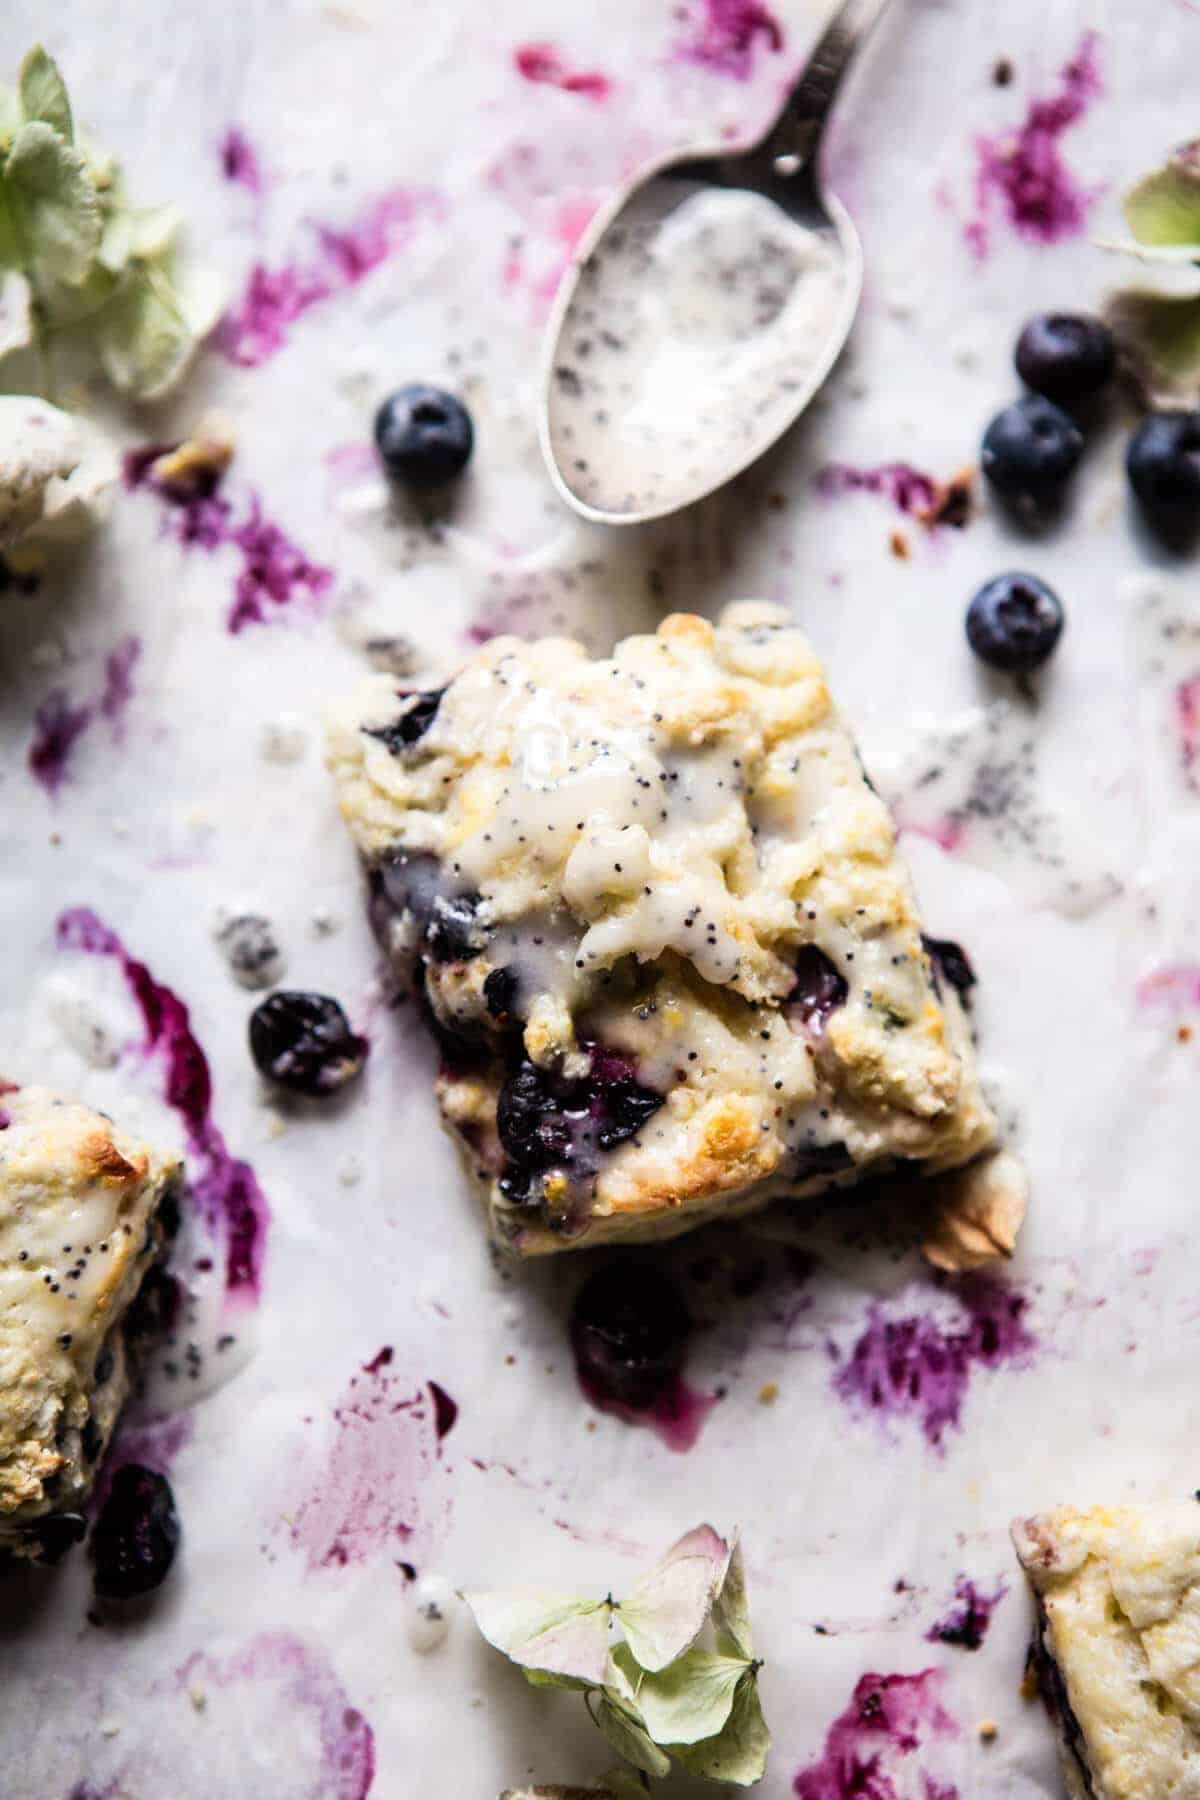
\includegraphics[width=1\textwidth,height=\textheight]{images/blueberry-lemon-poppy-seed-scones.jpg}

\textbf{Prep Time:} 10 min \textbar{} \textbf{Cook Time:} 20 min
\textbar{} \textbf{Total Time:} 30 min

\section{Ingredients}\label{ingredients-123}

\begin{itemize}
\tightlist
\item
  2 1/2 cups all-purpose flour
\item
  2 tablespoons granulated sugar
\item
  1 tablespoon baking powder
\item
  1/2 teaspoon salt
\item
  8 tablespoons cold unsalted butter, grated on a box grater just like
  cheese (1 stick)
\item
  1 egg
\item
  3/4 cup buttermilk + more for brushing
\item
  1 tablespoon vanilla extract
\item
  1 1/2 cups fresh or frozen blueberries
\item
  zest of 1/2 a lemon
\item
  1/2 cup powdered sugar, plus more if needed
\item
  2 tablespoons butter, melted
\item
  1/4 cup fresh lemon juice + reserve the zest
\item
  1/2 teaspoon vanilla extract
\item
  1-2 tablespoons poppy seeds
\end{itemize}

\section{Instructions}\label{instructions-123}

\begin{enumerate}
\def\labelenumi{\arabic{enumi}.}
\tightlist
\item
  Preheat the oven to 400 degrees F. Line 2 baking sheets with parchment
  paper.In a mixing bowl, combine the flour, sugar, baking powder, and
  salt. Add the butter and toss with the flour. Add the egg, buttermilk
  and vanilla. Mix until just combined, being careful not to overmix.
  Fold in the blueberries and lemon zest.Turn the dough onto a floured
  surface and then pat into 1-inch-thick square. Cut the dough into 2
  inch squares. Place pieces, about 2 inches apart on the prepared
  baking sheets. Brush each piece with buttermilk.Bake until golden
  brown, 15 to 18 minutes, rotating sheets halfway through. Let the
  scones cool slightly and then drizzle with the lemon poppy seed glaze
  (see below). Serve warm with butter.
\end{enumerate}

\bookmarksetup{startatroot}

\chapter{Roasted Cauliflower Fried Halloumi Tacos with Spicy Avocado
Basil
Guacamole}\label{roasted-cauliflower-fried-halloumi-tacos-with-spicy-avocado-basil-guacamole}

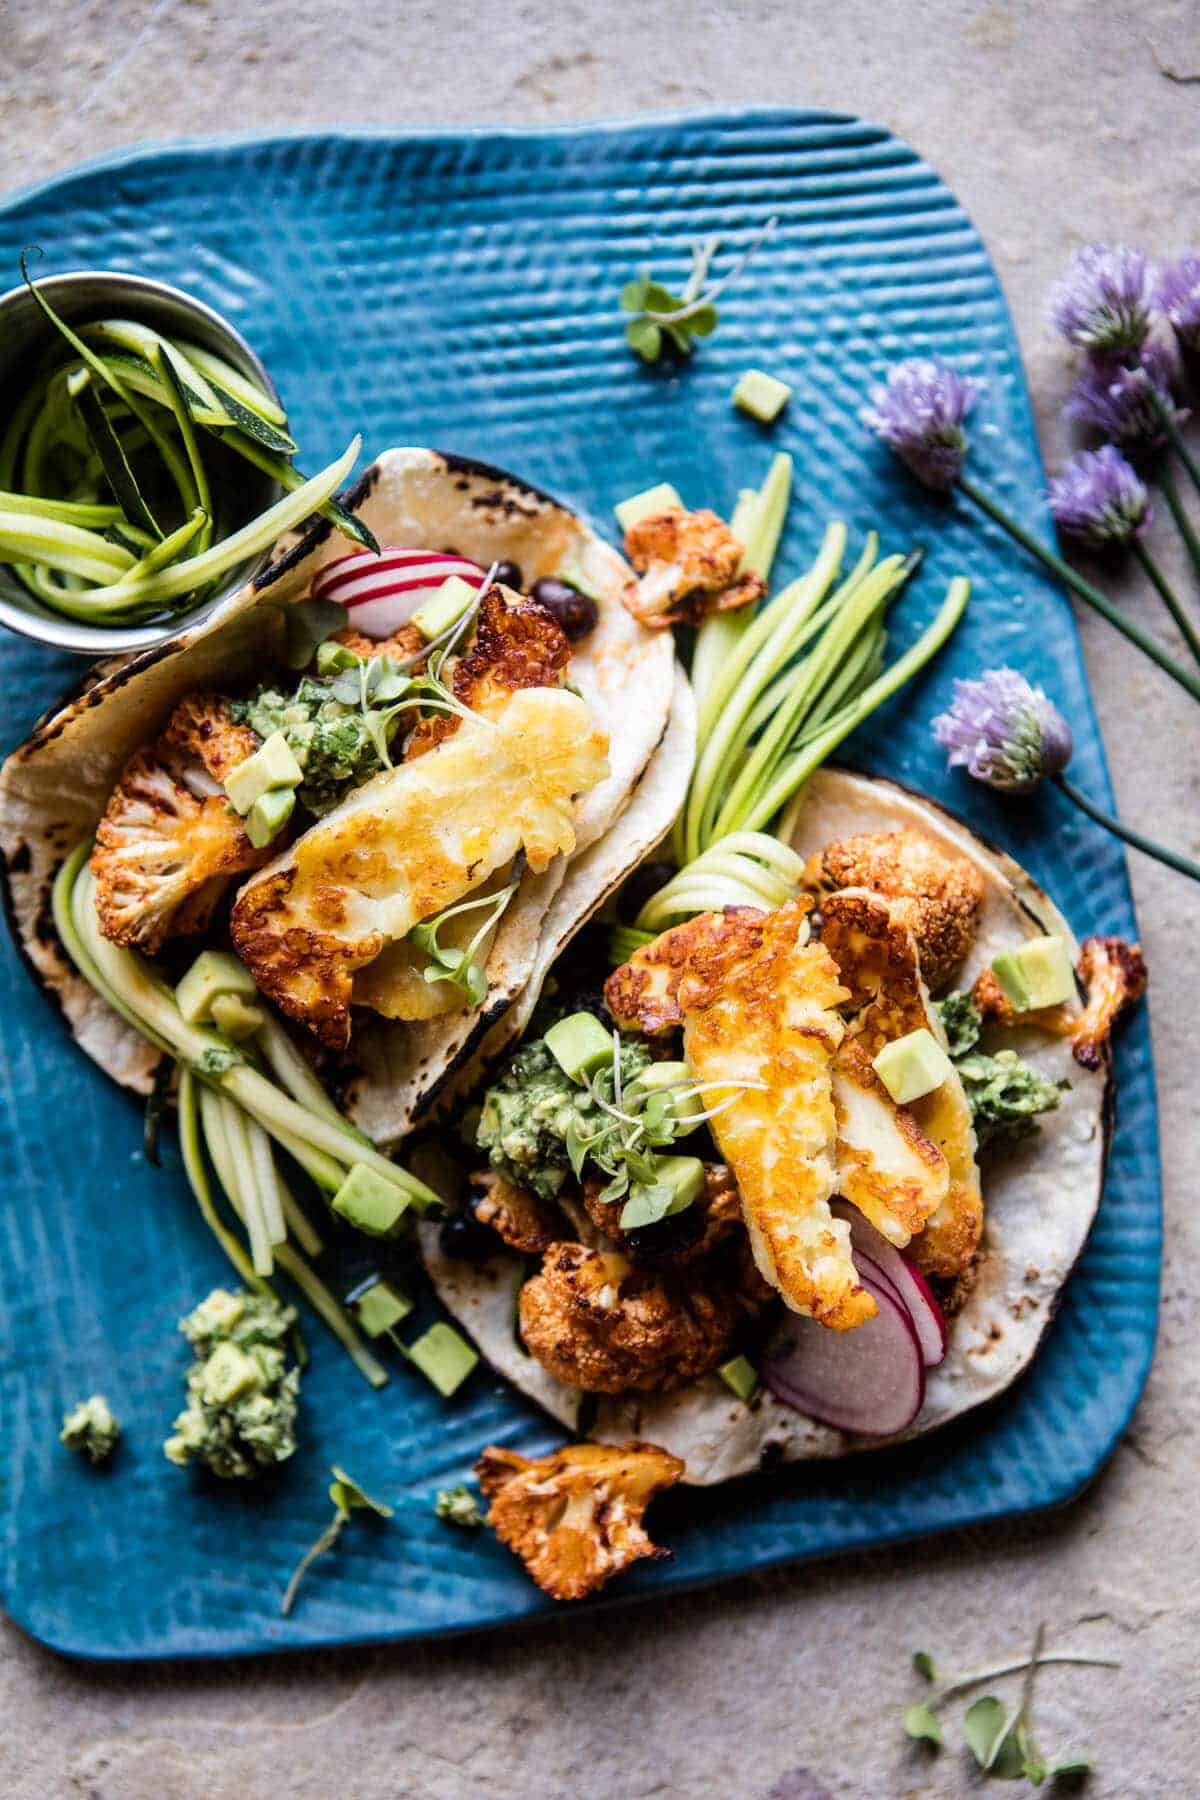
\includegraphics[width=1\textwidth,height=\textheight]{images/roasted-cauliflower-fried-halloumi-tacos-with-spicy-avocado-basil-guacamole.jpg}

\textbf{Prep Time:} 15 min \textbar{} \textbf{Cook Time:} 20 min
\textbar{} \textbf{Total Time:} 35 min

\section{Ingredients}\label{ingredients-124}

\begin{itemize}
\tightlist
\item
  1 large, or 2 small, heads cauliflower, cut into florets
\item
  2 tablespoons sesame or olive oil
\item
  2 teaspoons smoked paprika
\item
  1 teaspoon chili powder
\item
  1 teaspoon cumin
\item
  1 teaspoon kosher salt and pepper
\item
  1 (14 ounce) can black beans, drained and rinsed
\item
  8 ounces halloumi cheese, sliced
\item
  1 cucumber or zucchini, shredded
\item
  1 avocado, halved
\item
  1 cup fresh basil
\item
  1/4 cup toasted pine nuts
\item
  1 jalapeno
\item
  juice of 1 lemon
\item
  2 tablespoons sesame oil
\item
  kosher salt and pepper
\end{itemize}

\section{Instructions}\label{instructions-124}

\begin{enumerate}
\def\labelenumi{\arabic{enumi}.}
\tightlist
\item
  Preheat the oven to 400 degrees F.
\item
  On a baking sheet, toss together the cauliflower, oil, paprika, chili
  powder, cumin, salt and pepper. Transfer to the oven and roast for
  20-30 minutes, tossing halfway through cooking. Remove from the oven
  and stir in the black beans.
\item
  Meanwhile, make the avocado guacamole. Add half the avocado, basil,
  pine nuts, jalapeño (remove seeds for less heat), lemon juice and oil
  to a food processor and pulse until chunky smooth. Dice the remaining
  avocado half and stir into the pesto. Taste and season with salt and
  pepper.
\item
  Heat a small skillet over medium heat and add a drizzle of olive oil.
  Once hot, add the Halloumi slices and cook for 1-2 minutes per side or
  until lightly golden. Remove and drain onto paper towels.
\item
  To assemble, layer the cucumber, zucchini, and cauliflower in the
  tortillas. Top with fried cheese and guacamole. Enjoy!!
\end{enumerate}

\bookmarksetup{startatroot}

\chapter{Super Green Pea and Asparagus Burrata
Pizza}\label{super-green-pea-and-asparagus-burrata-pizza}

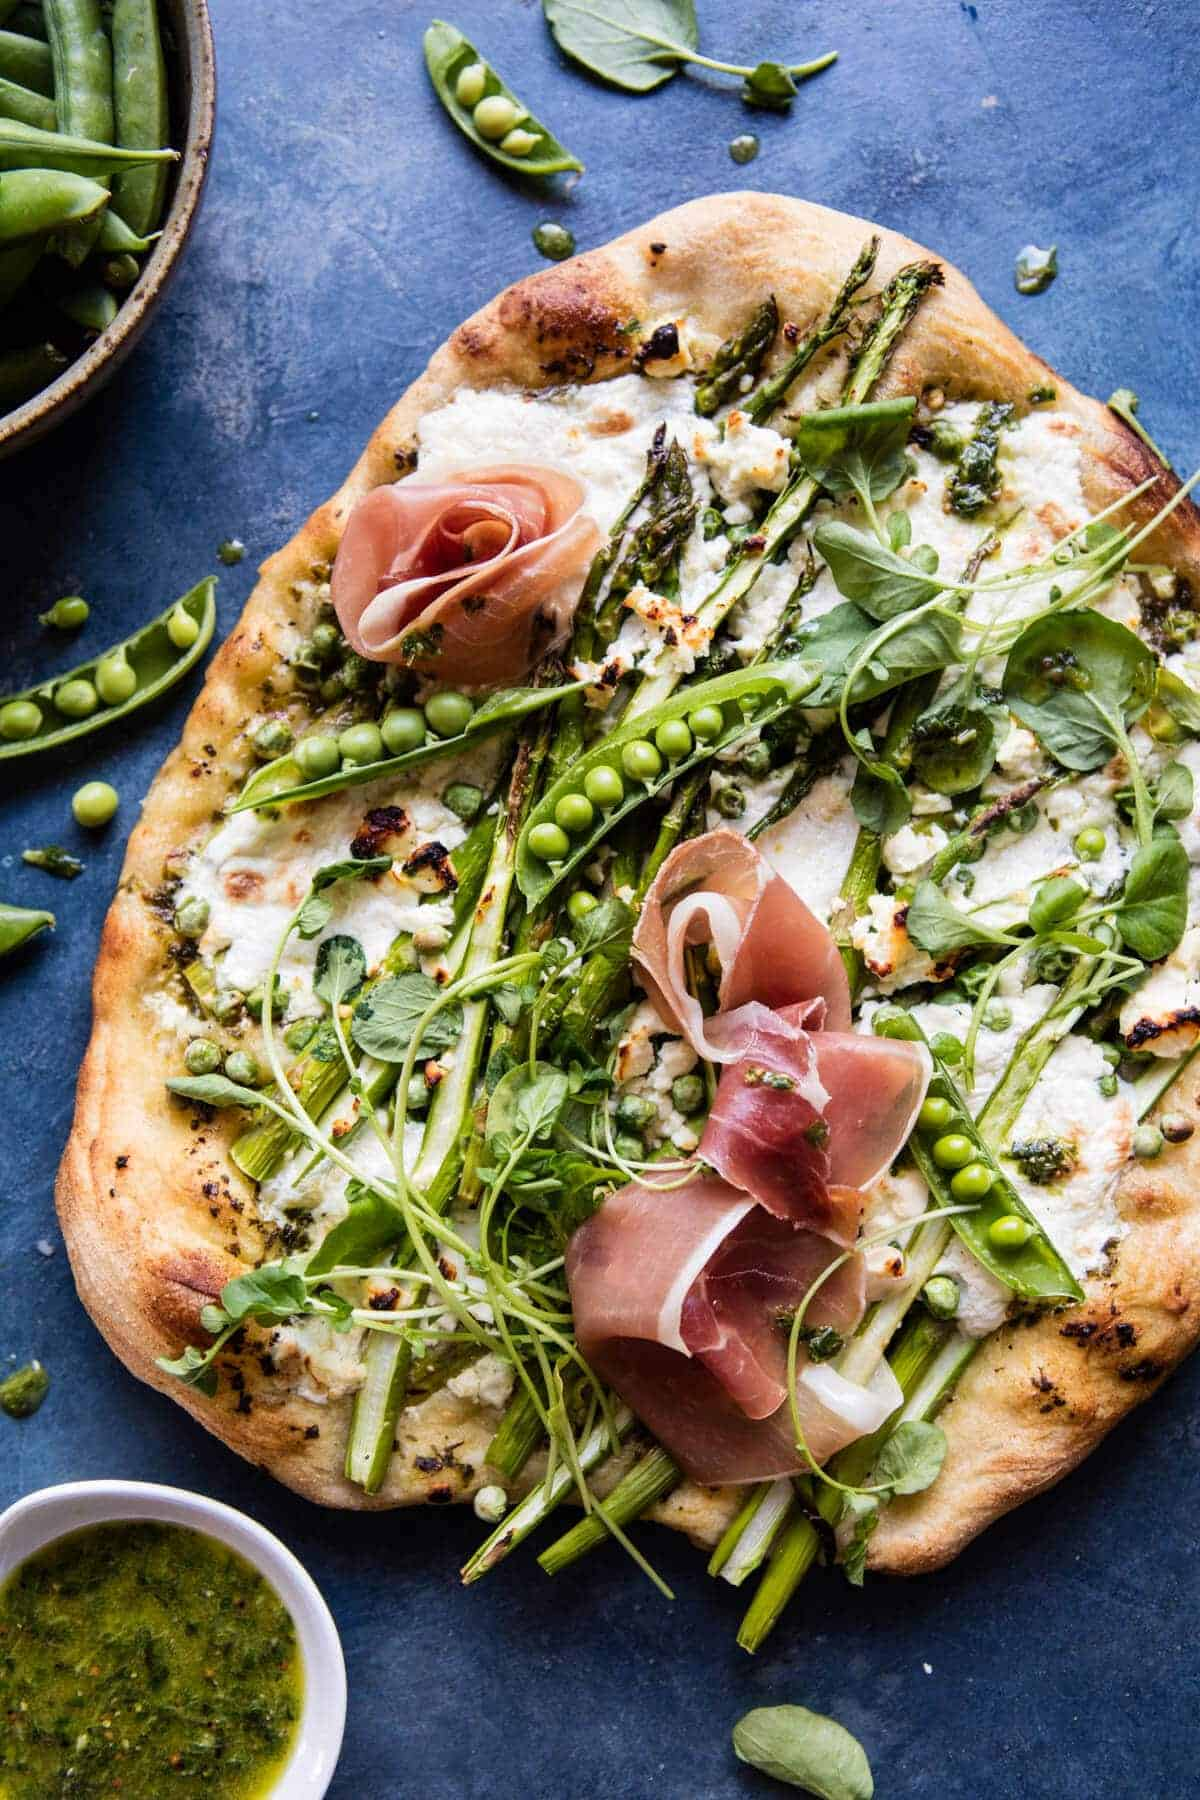
\includegraphics[width=1\textwidth,height=\textheight]{images/super-green-pea-and-asparagus-burrata-pizza.jpg}

\textbf{Prep Time:} 10 min \textbar{} \textbf{Cook Time:} 10 min
\textbar{} \textbf{Total Time:} 20 min

\section{Ingredients}\label{ingredients-125}

\begin{itemize}
\tightlist
\item
  1/3 cup olive oil
\item
  juice + zest of 2 lemons
\item
  1/4 cup fresh basil
\item
  1 tablespoon dijon mustard
\item
  1 teaspoon kosher salt and pepper
\item
  1/2 pound homemade or store-bought pizza dough
\item
  1/2 cup crumbled feta cheese
\item
  1 small bunch asparagus, cut in half lengthwise
\item
  1 cup fresh sugar snap peas or frozen peas
\item
  8 ounces burrata cheese
\item
  6 ounces thinly sliced prosciutto
\item
  1 handful of sprouts or watercress
\item
  1 tablespoon chopped fresh chives
\item
  crushed red pepper flakes, for sprinkling
\end{itemize}

\section{Instructions}\label{instructions-125}

\begin{enumerate}
\def\labelenumi{\arabic{enumi}.}
\tightlist
\item
\end{enumerate}

\bookmarksetup{startatroot}

\chapter{Morning Glory Power
Smoothie}\label{morning-glory-power-smoothie}

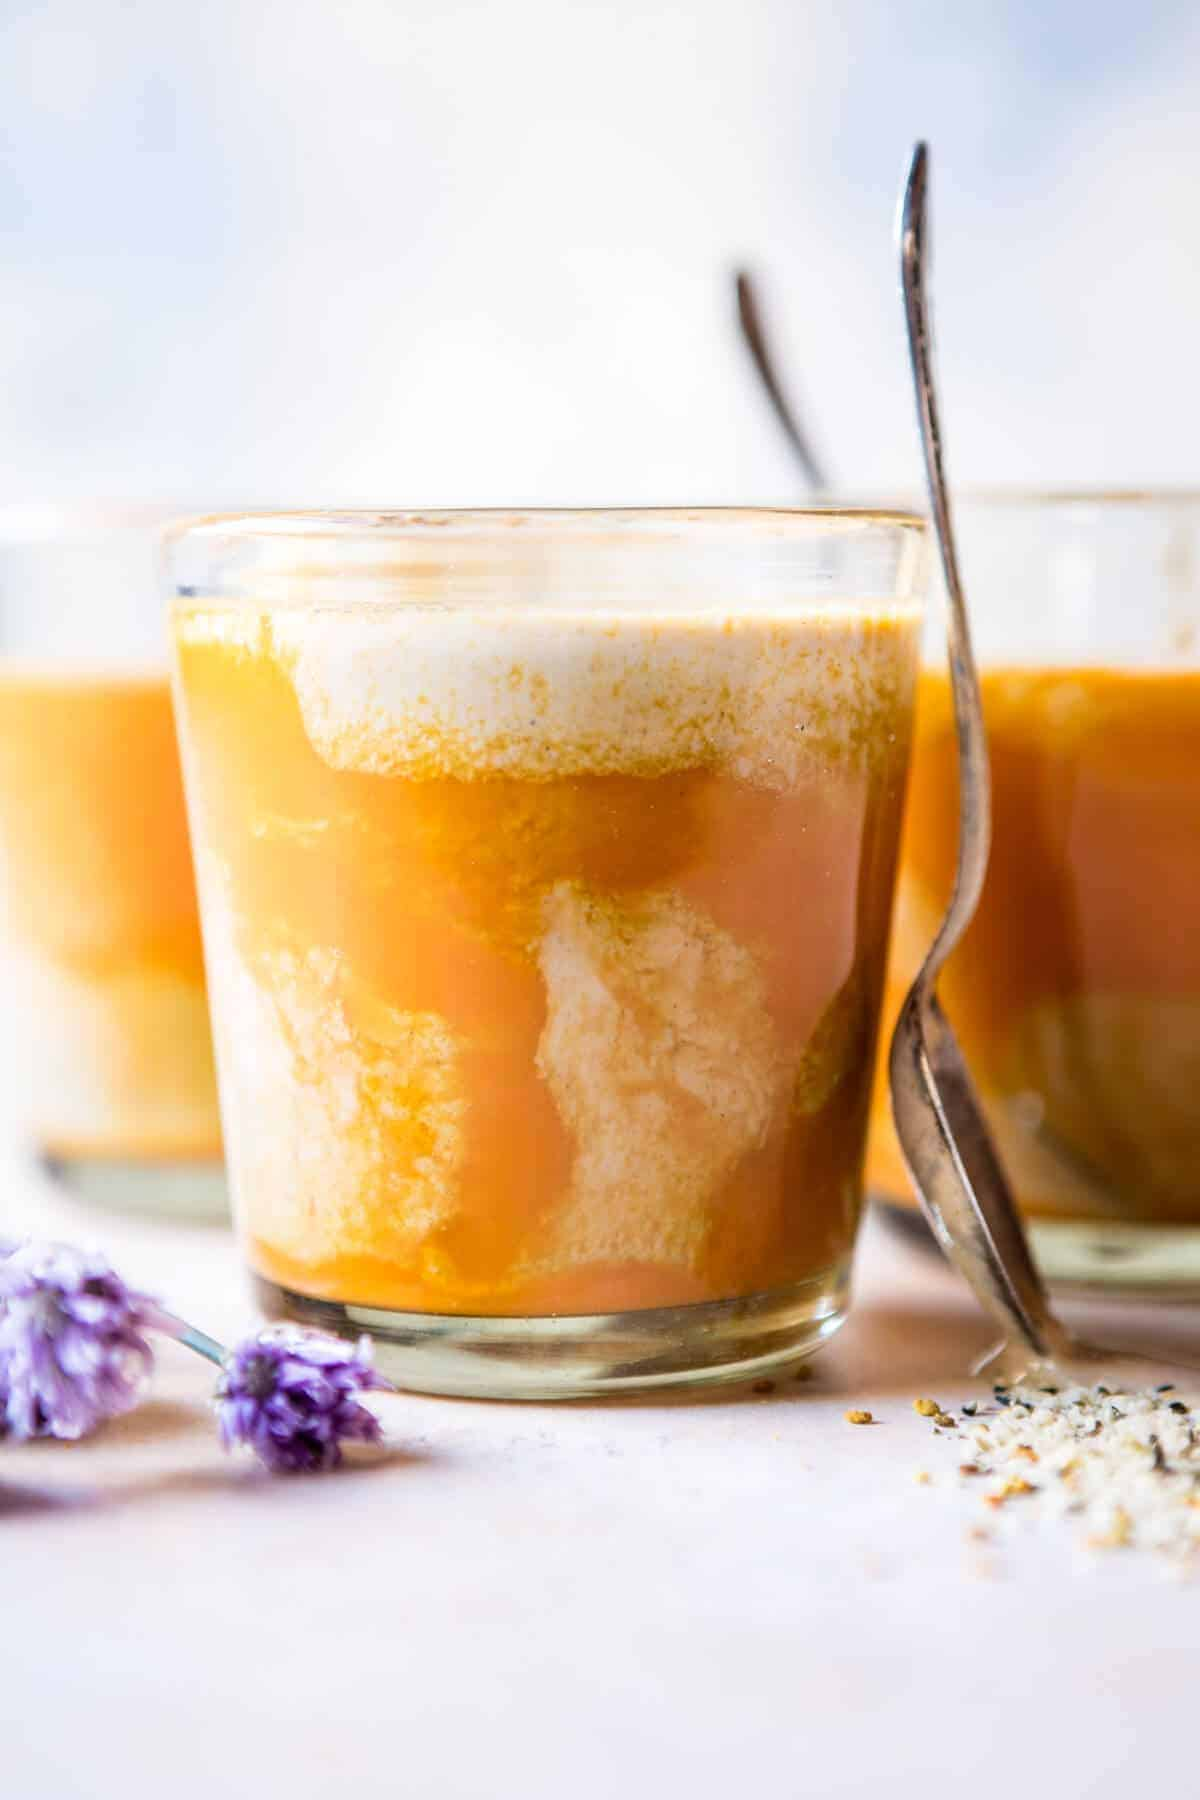
\includegraphics[width=1\textwidth,height=\textheight]{images/morning-glory-power-smoothie.jpg}

\textbf{Prep Time:} 10 min \textbar{} \textbf{Cook Time:} \textbar{}
\textbf{Total Time:} 10 min

\section{Ingredients}\label{ingredients-126}

\begin{itemize}
\tightlist
\item
  1 small carrot, rough chopped
\item
  1/2 teaspoon turmeric
\item
  1/2 cup coconut water or orange juice
\item
  1 fresh or frozen banana
\item
  1-2 dates, pitted
\item
  2 tablespoons raw walnuts or cashews, soaked overnight in water
\item
  1 tablespoon hemp seeds
\item
  1 teaspoon maca powder
\item
  1/2 teaspoon cinnamon
\item
  1 teaspoon vanilla extract
\item
  1 1/2 -2 cups coconut or almond milk
\end{itemize}

\section{Instructions}\label{instructions-126}

\begin{enumerate}
\def\labelenumi{\arabic{enumi}.}
\tightlist
\item
  In a blender, combine the carrot, turmeric, and coconut water. Blend
  until completely smooth and no carrot chunks remain, adding water if
  needed to thin. Pour into a tall glass2. Rinse the blender out.
  Combine the banana, dates, nuts, hemp seeds, maca powder, cinnamon,
  vanilla, and milk. Blend until smooth and creamy, adding milk if
  needed to reach your desired consistency. Pour over the carrot mixture
  and stir gently to swirl. Enjoy!
\end{enumerate}

\bookmarksetup{startatroot}

\chapter{Coconut Lime Chicken Curry with Rice
Noodles}\label{coconut-lime-chicken-curry-with-rice-noodles}

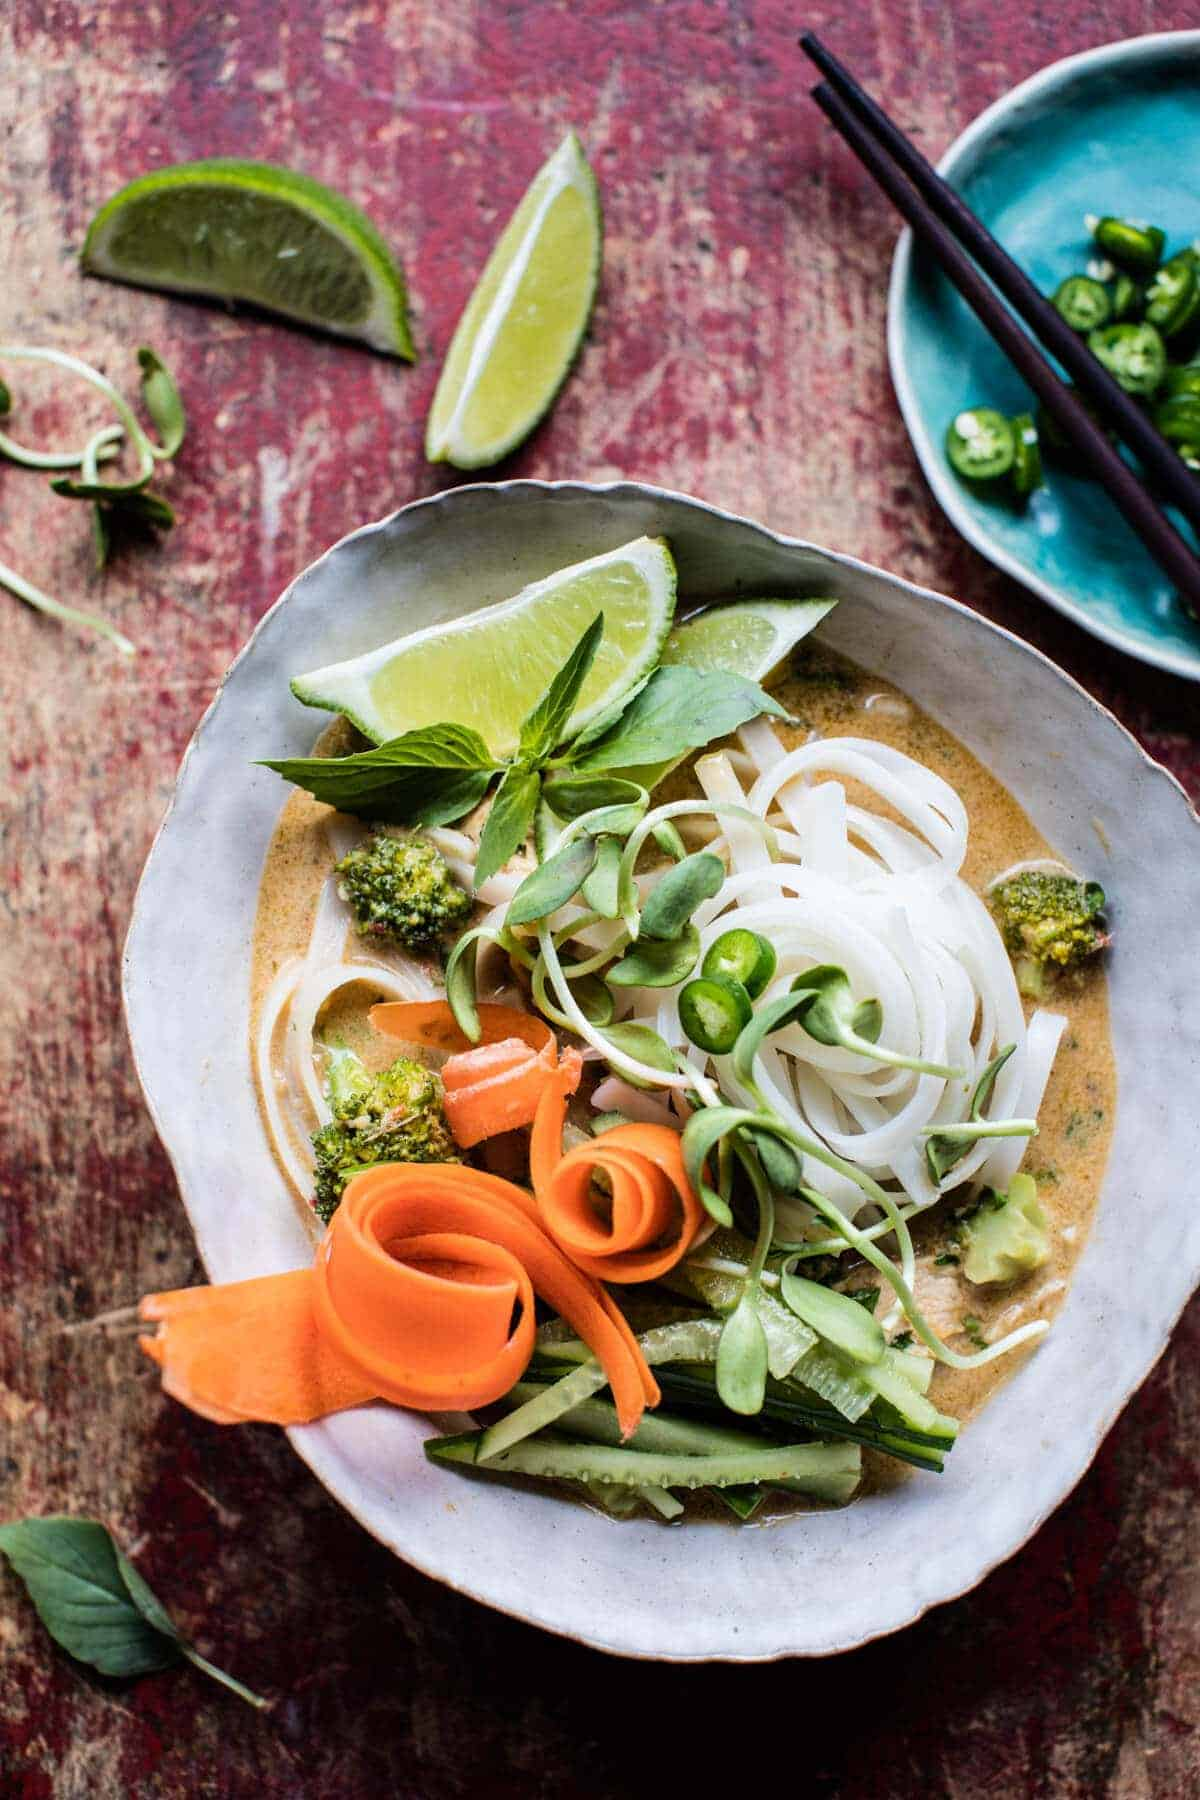
\includegraphics[width=1\textwidth,height=\textheight]{images/coconut-lime-chicken-curry-with-rice-noodles.jpg}

\textbf{Prep Time:} 10 min \textbar{} \textbf{Cook Time:} 30 min
\textbar{} \textbf{Total Time:} 40 min

\section{Ingredients}\label{ingredients-127}

\begin{itemize}
\tightlist
\item
  1/2 sweet onion, quartered
\item
  2 stalks lemongrass, roughly chopped
\item
  1 red fresno pepper, seeded
\item
  1 inch piece fresh ginger, peeled
\item
  2 cloves garlic, chopped
\item
  2 tablespoons Thai red or green curry paste
\item
  2 tablespoons peanut or sesame oil
\item
  1 pound boneless chicken breasts, cut into bite size pieces
\item
  2-3 cups Almond Breeze Unsweetened Original Almondmilk Coconutmilk
  Blend
\item
  2 tablespoons fish sauce
\item
  1 bunch broccoli, ends trimmed
\item
  8 ounces rice noodles
\item
  juice of 2 limes
\item
  1/4 cup fresh cilantro, chopped
\item
  1/4 cup fresh basil, chopped, plus more for serving
\item
  2 persian cucumbers, sliced
\item
  sprouts, shredded coconut, shredded carrots, for serving
\end{itemize}

\section{Instructions}\label{instructions-127}

\begin{enumerate}
\def\labelenumi{\arabic{enumi}.}
\tightlist
\item
  In a blender or food processor, combine the onion, lemongrass, fresno
  pepper, ginger, garlic, and curry paste and pulse until a paste forms.
\item
  Heat the oil in a large pot set over medium heat. When the oil
  shimmers, add the curry paste mixture and cook until fragrant, about
  2-3 minutes. Stir in the chicken and cook another 2-3 minutes until
  browned.
\item
  Pour in the Coconut Almondmilk. Add the fish sauce and broccoli. Bring
  the mix to a simmer over medium heat and then reduce the heat to
  medium low and simmer 20-25 minutes or until the chicken is cooked
  through and the sauce has thickened slightly.
\item
  When the curry is done, remove from the heat and stir in the lime
  juice, cilantro and basil.
\item
  To serve, divide the noodles among bowls and ladle the curry over top.
  Garnish with the cucumbers, fresh basil, sprouts, carrots, and lime.
  Enjoy!
\end{enumerate}

\bookmarksetup{startatroot}

\chapter{Crispy Baked Basil Chicken Cordon
Bleu}\label{crispy-baked-basil-chicken-cordon-bleu}

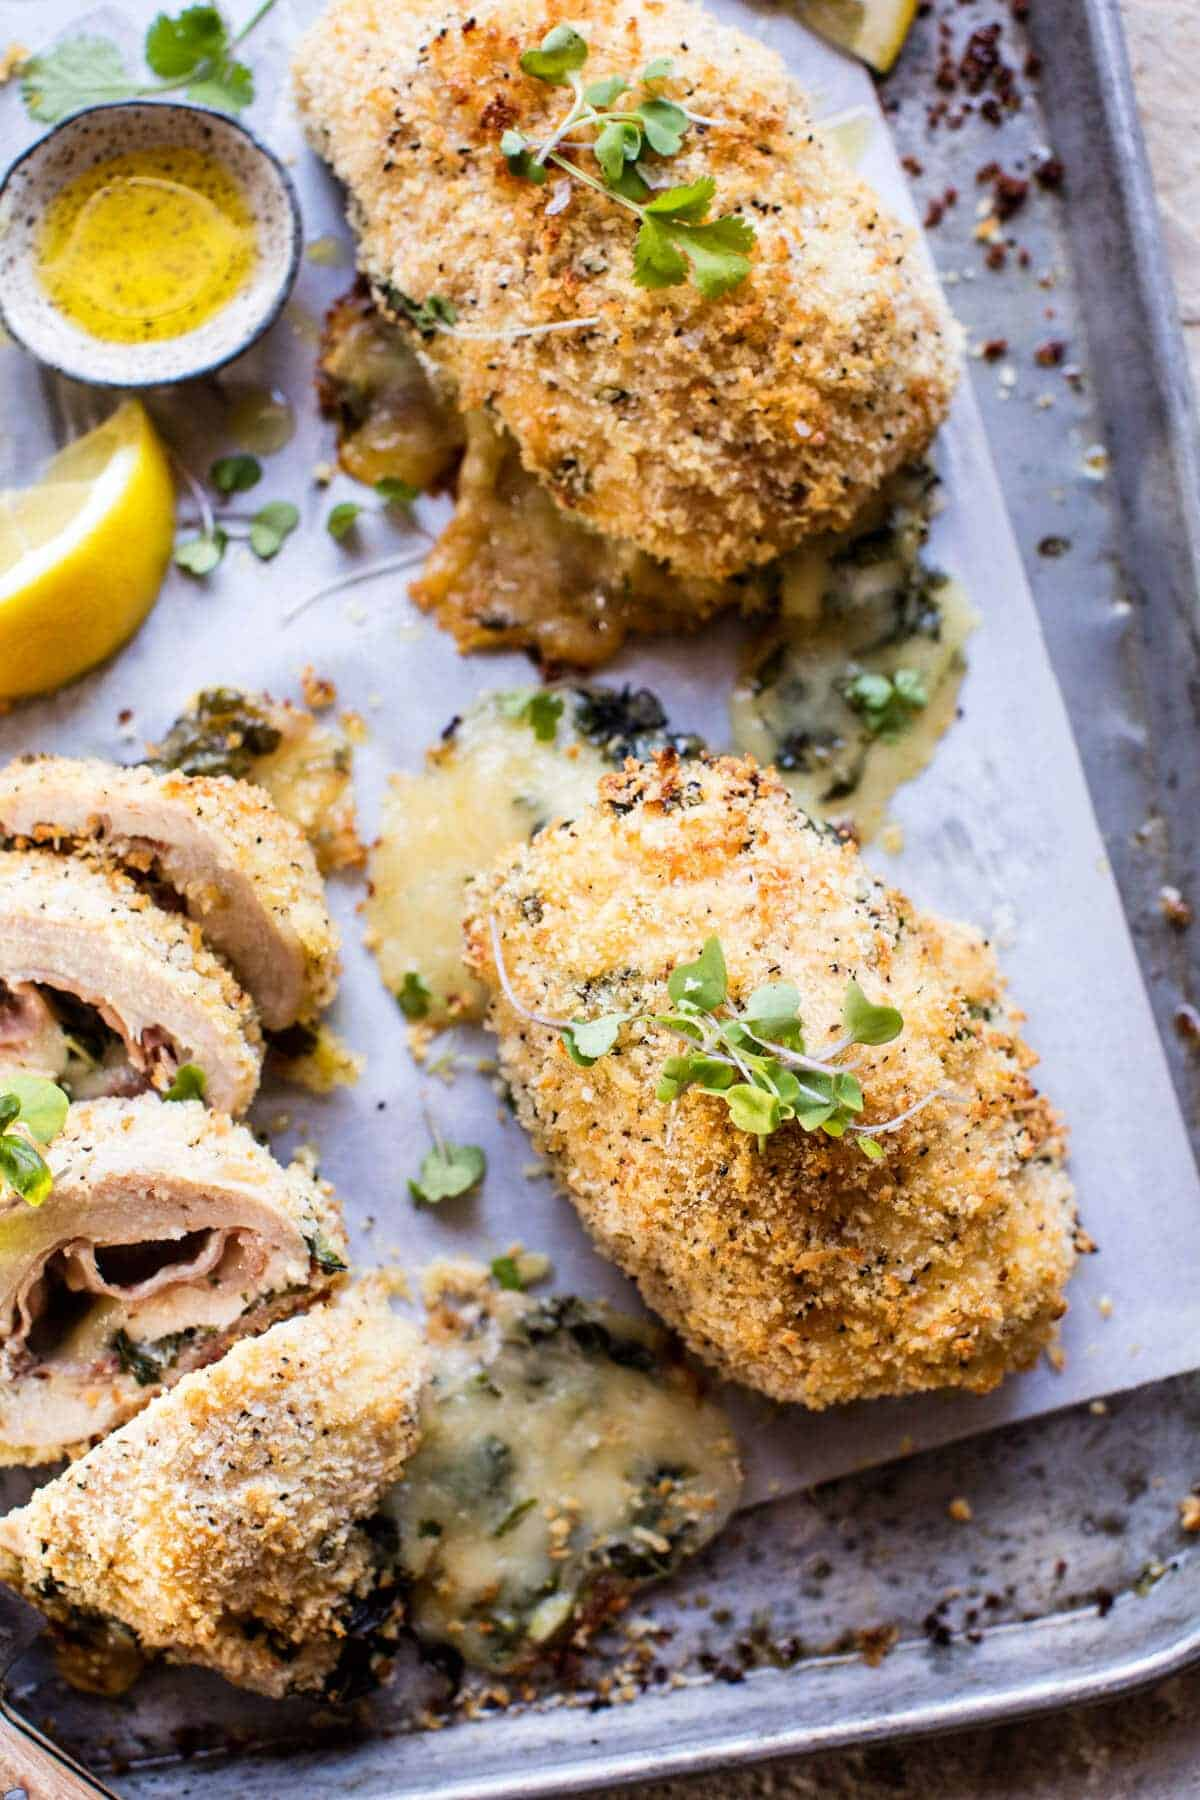
\includegraphics[width=1\textwidth,height=\textheight]{images/crispy-baked-basil-chicken-cordon-bleu.jpg}

\textbf{Prep Time:} 15 min \textbar{} \textbf{Cook Time:} 25 min
\textbar{} \textbf{Total Time:} 40 min

\section{Ingredients}\label{ingredients-128}

\begin{itemize}
\tightlist
\item
  4 skinless chicken breasts
\item
  kosher salt and pepper
\item
  4 thin slices prosciutto
\item
  1/2 cup shredded swiss cheese
\item
  1/2 cup shredded fontina cheese
\item
  1 cup fresh basil, chopped
\item
  2 eggs, beaten
\item
  1 1/2 cups panko bread crumbs
\item
  1/2 teaspoon garlic powder
\item
  crushed red pepper flakes
\item
  olive oil, for drizzling
\item
  lemons and fresh basil, for serving
\end{itemize}

\section{Instructions}\label{instructions-128}

\begin{enumerate}
\def\labelenumi{\arabic{enumi}.}
\tightlist
\item
  Preheat the oven to 400 degrees F. Lightly grease a baking sheet with
  oil.
\item
  Layer the chicken flat on a piece of plastic wrap and pound the
  chicken into about 1/4 inch thickness. Season with salt and pepper.
\item
  Layer each piece of chicken with 1 slice prosciutto, a little of each
  type of cheese, and a few basil leaves. Roll the chicken up and place
  seam side down on the prepared baking sheet.
\item
  Add the eggs to a shallow bowl. To another bowl, add the bread crumbs,
  garlic powder, and a pinch each of crushed red pepper flakes, salt and
  pepper.
\item
  Working with 1 piece of chicken at a time, dip the chicken through the
  eggs and then dredge through the bread crumb seasoning. Place back on
  the baking sheet and repeat with the remaining chicken.
\item
  Drizzle the chicken lightly with olive oil and transfer to the oven.
  Bake for 25-30 minutes or until the chicken is cooked through. Serve
  with lemon and basil. Enjoy!
\end{enumerate}

\bookmarksetup{startatroot}

\chapter{Raw Chocolate Banana Cashew Cream Pie
Bars}\label{raw-chocolate-banana-cashew-cream-pie-bars}

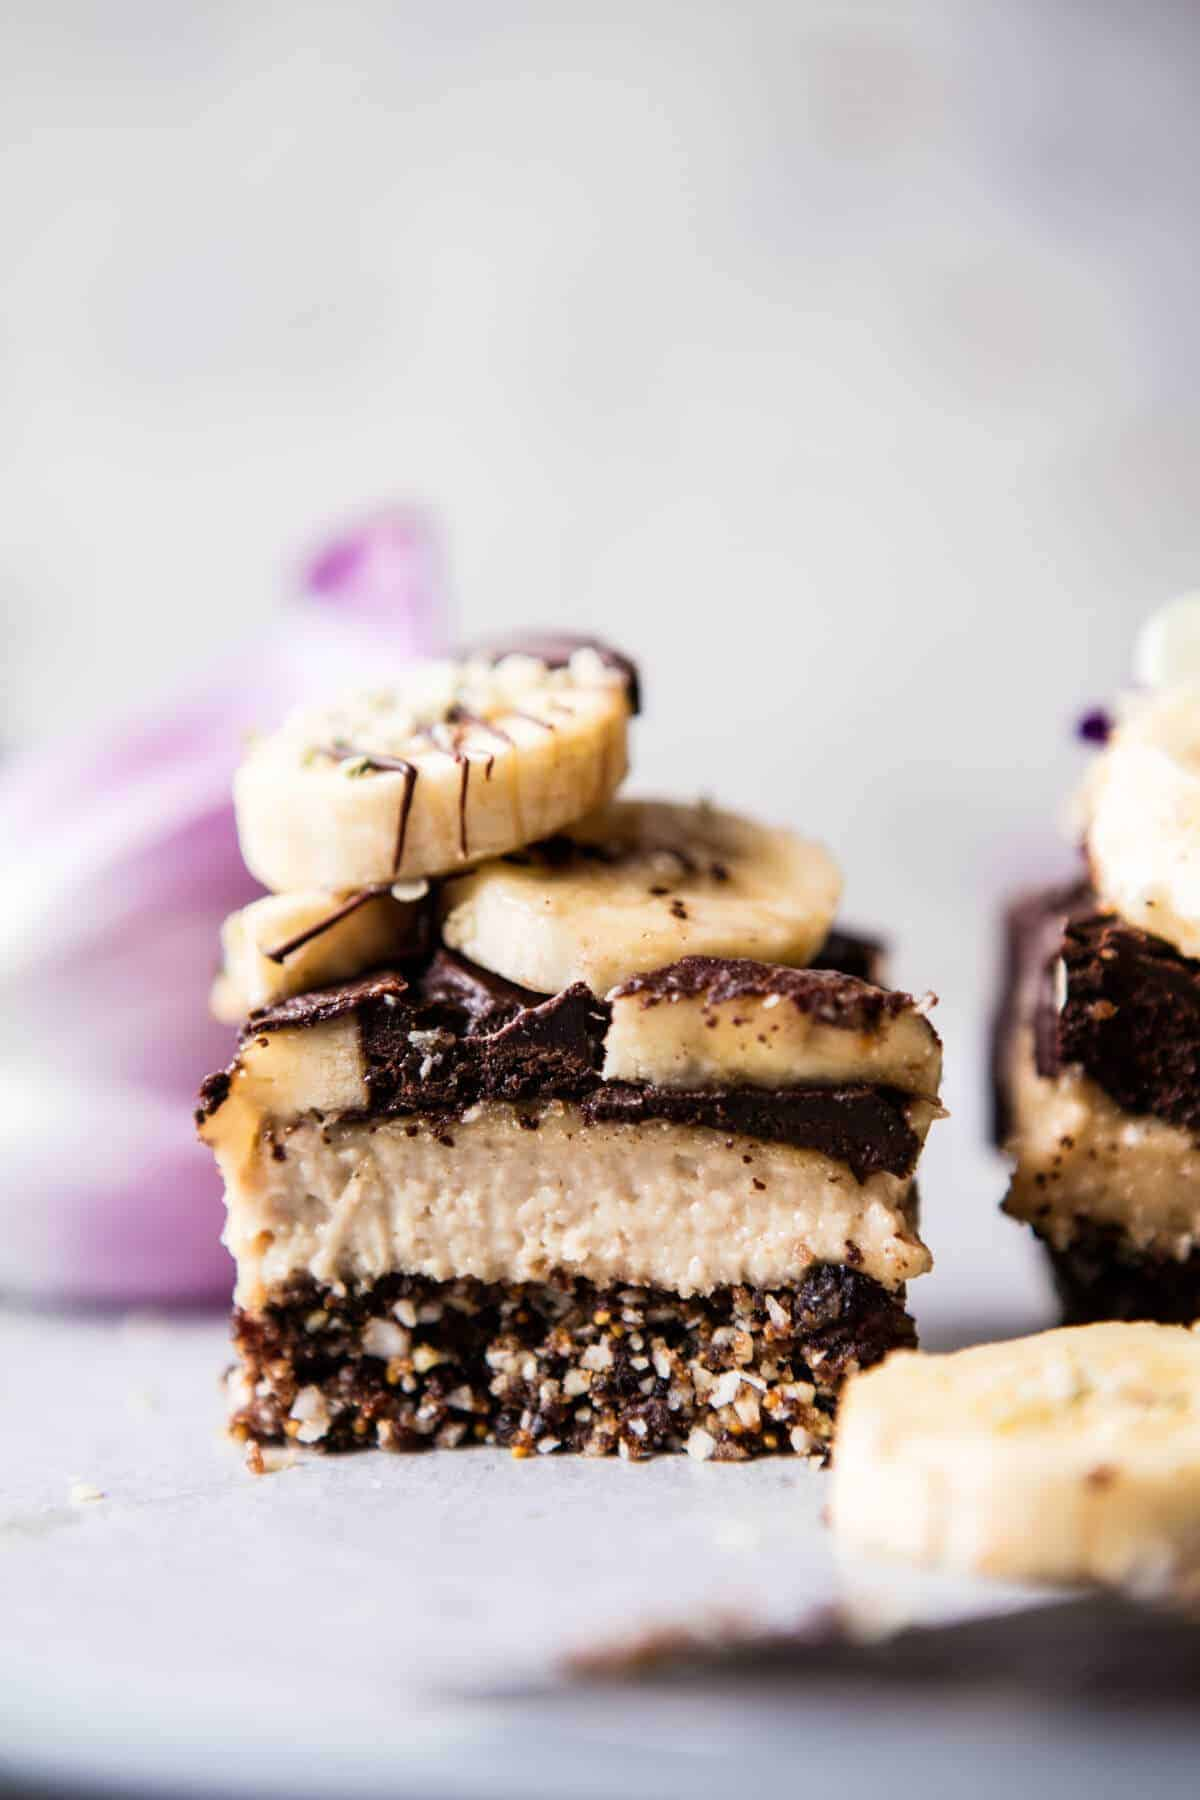
\includegraphics[width=1\textwidth,height=\textheight]{images/raw-chocolate-banana-cashew-cream-pie-bars.jpg}

\textbf{Prep Time:} 20 min \textbar{} \textbf{Cook Time:} \textbar{}
\textbf{Total Time:} 20 min

\section{Ingredients}\label{ingredients-129}

\begin{itemize}
\tightlist
\item
  1 cup raw pecans
\item
  2 cups raw unsweetened coconut
\item
  1 cup pitted packed dates
\item
  2 teaspoons vanilla extract
\item
  pinch of flaky sea salt
\item
  2 cups roasted cashews
\item
  2-4 ripe, but firm bananas, sliced
\item
  1/2 cup coconut oil, melted
\item
  1 cup cocoa or cacao powder
\item
  1/3 cup honey, more or less to taste
\item
  hemp or sesame seeds, for topping optional
\end{itemize}

\section{Instructions}\label{instructions-129}

\begin{enumerate}
\def\labelenumi{\arabic{enumi}.}
\tightlist
\item
  Line an 8x8 inch square baking pan with parchment paper.
\item
  In the bowl of a food processor, combine the pecans, 1 cup coconut,
  dates, 1 teaspoon vanilla, and pinch of salt. Pulse until finely
  chopped and easily holds together when squeezed in your hand. Press
  the base mixture into the prepared pan. Place the pan in the freezer.
\item
  Going back to the bowl of your food processor (no need to clean it!),
  combine the cashews, remaining 1 cup coconut, 1/2 cup water, and
  remaining 1 teaspoon vanilla. Pulse until smooth and creamy. Remove
  the base layer from the freezer and add the cashew cream in an even
  layer. Top with sliced bananas.
\item
  In a separate bowl, whisk together the melted coconut oil, cocoa and
  honey. Pour the chocolate mixture over the bananas. Place in the
  fridge and chill until firm, at least 1 hour.
\item
  Cut into bars and serve topped with fresh bananas and seeds. Keep bars
  stored in the fridge.
\end{enumerate}

\bookmarksetup{startatroot}

\chapter{Mango Avocado Soba Noodles with Sesame Salmon
Poke}\label{mango-avocado-soba-noodles-with-sesame-salmon-poke}

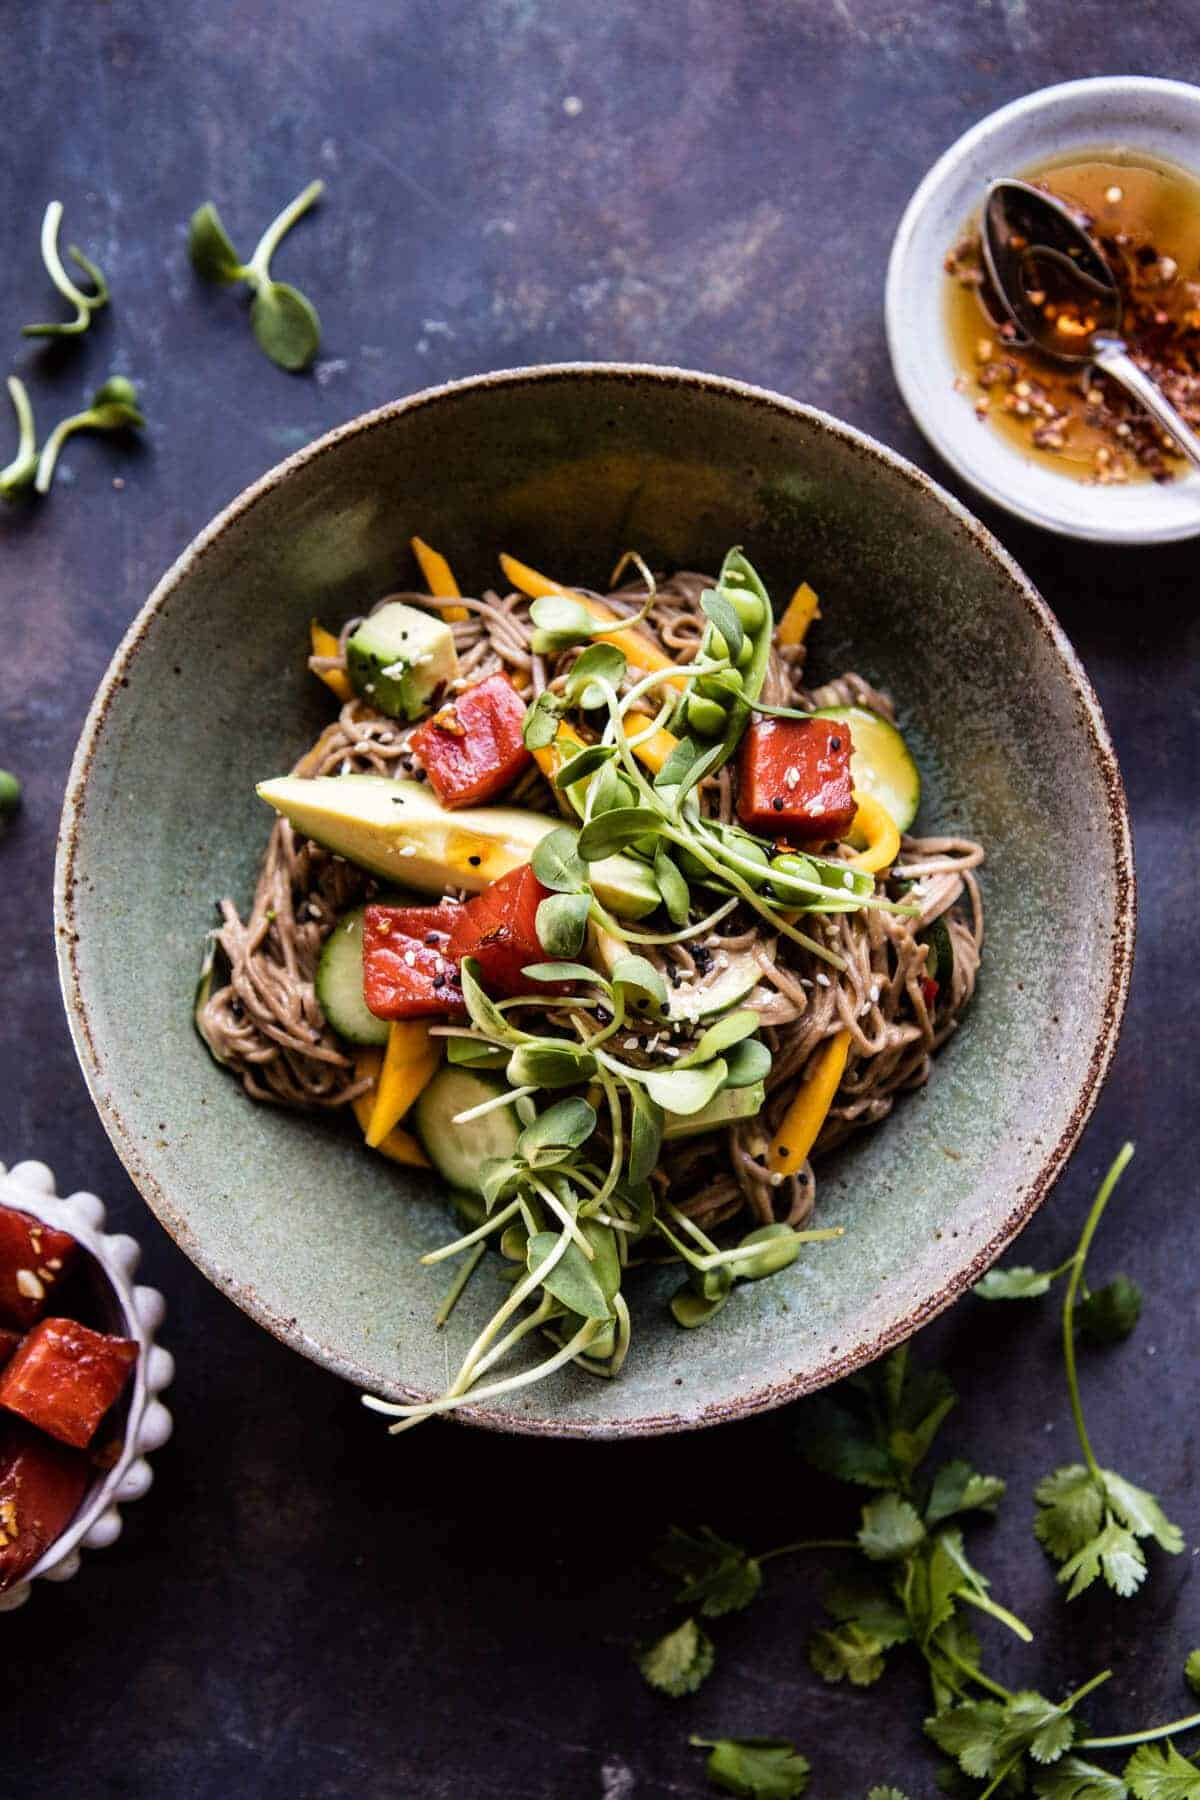
\includegraphics[width=1\textwidth,height=\textheight]{images/mango-avocado-soba-noodles-with-sesame-salmon-poke.jpg}

\textbf{Prep Time:} 15 min \textbar{} \textbf{Cook Time:} 5 min
\textbar{} \textbf{Total Time:} 20 min

\section{Ingredients}\label{ingredients-130}

\begin{itemize}
\tightlist
\item
  1/4 cup low-sodium soy sauce
\item
  1 tablespoon rice wine vinegar
\item
  1 tablespoon honey
\item
  1 inch fresh ginger, grated
\item
  1 clove garlic, minced or grated
\item
  1 pound sushi grade salmon (cut into chunks)
\item
  12 ounces soba noodles
\item
  3 tablespoons sesame oil
\item
  4 green onions, chopped
\item
  1/4 cup tahini
\item
  juice of 1/2 a lemon
\item
  2 tablespoons oyster sauce
\item
  1 mango, cut into matchsticks
\item
  1 cup snap peas
\item
  1 avocado, diced
\item
  1 Persian cucumber, sliced
\item
  sprouts, sesame seeds, and or hot chili sauce for serving
\end{itemize}

\section{Instructions}\label{instructions-130}

\begin{enumerate}
\def\labelenumi{\arabic{enumi}.}
\tightlist
\item
\end{enumerate}

\bookmarksetup{startatroot}

\chapter{Earl Grey Blueberry Oatmeal}\label{earl-grey-blueberry-oatmeal}

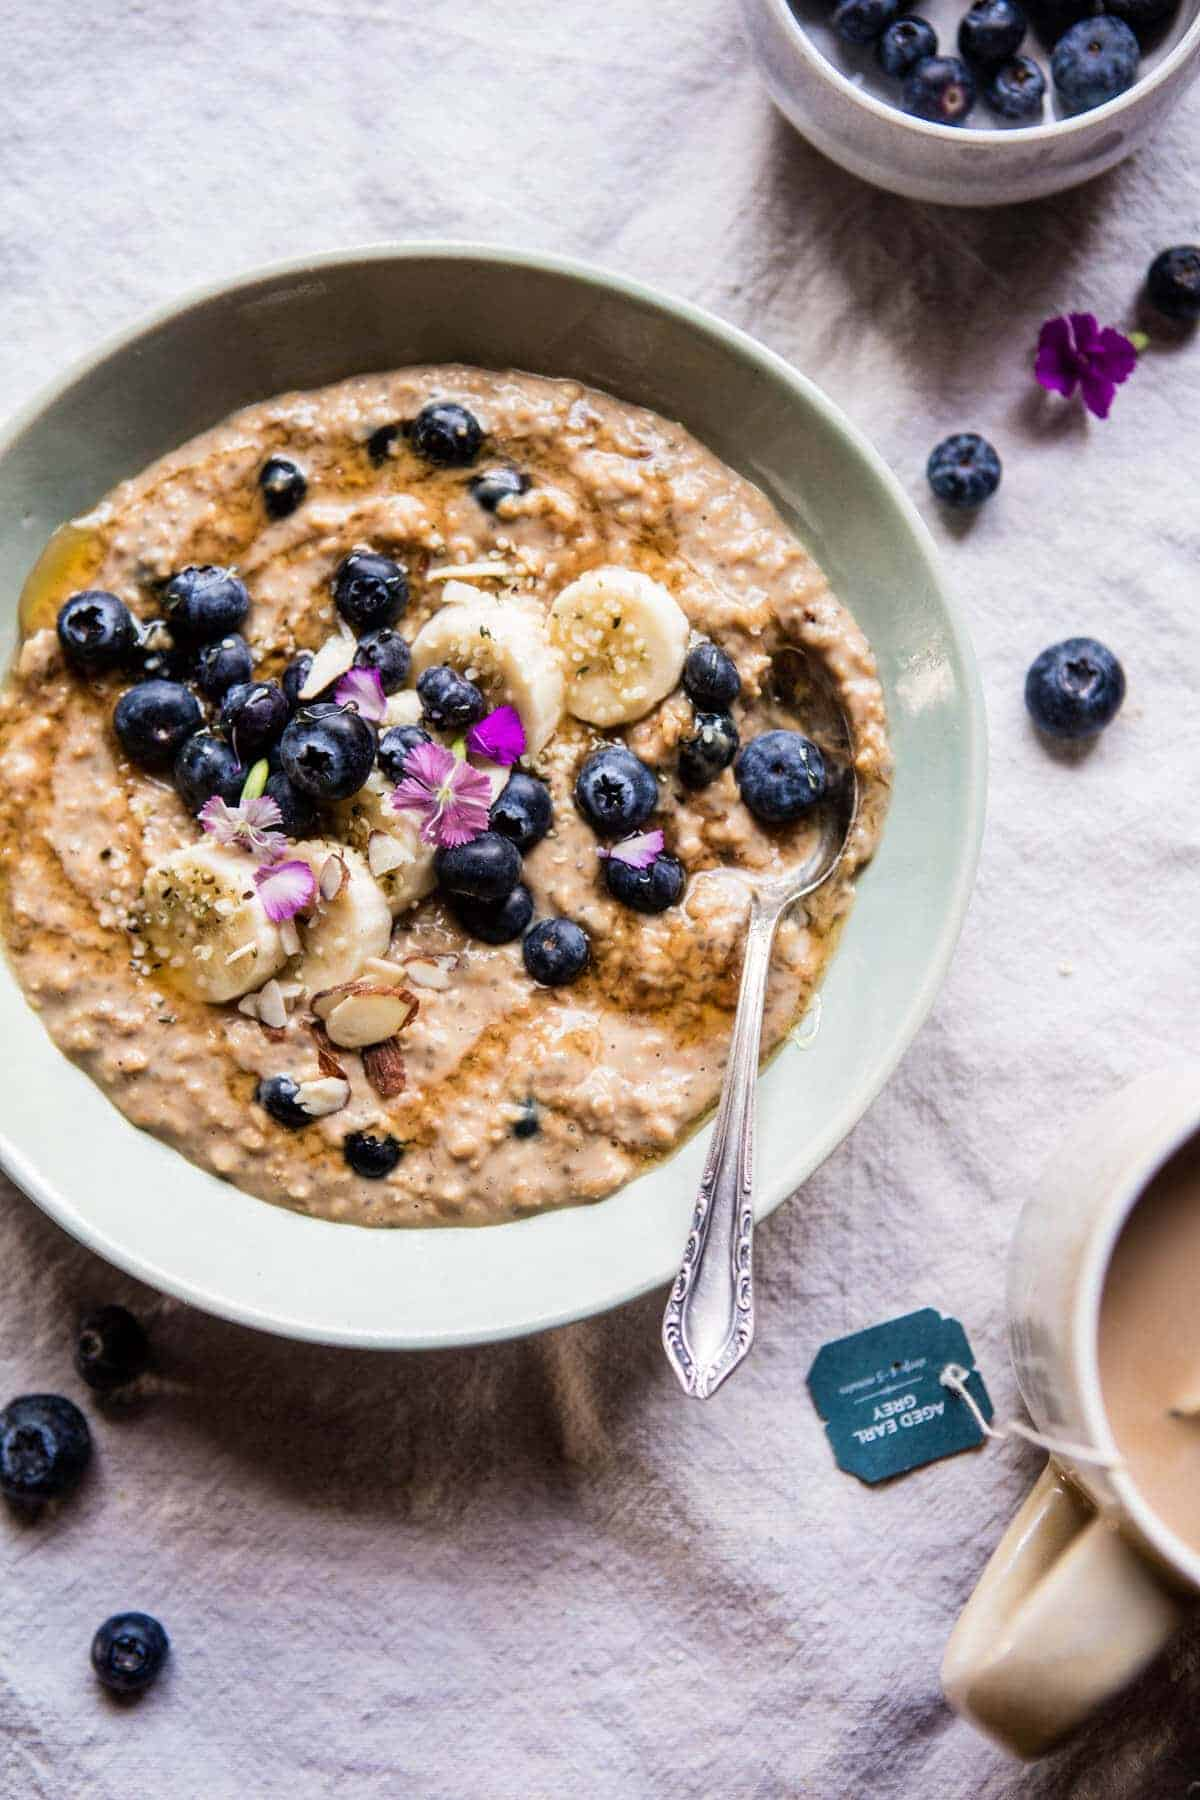
\includegraphics[width=1\textwidth,height=\textheight]{images/earl-grey-blueberry-oatmeal.jpg}

\textbf{Prep Time:} 10 min \textbar{} \textbf{Cook Time:} 5 min
\textbar{} \textbf{Total Time:} 15 min

\section{Ingredients}\label{ingredients-131}

\begin{itemize}
\tightlist
\item
  1/2 cup milk
\item
  1 earl grey tea bag
\item
  1 packet Pure Growth Organic Original Oatmeal
\item
  1/4 cup fresh blueberries, plus more for serving
\item
  1 tablespoon chia seeds
\item
  1 tablespoon honey
\item
  1/2 teaspoon vanilla extract
\item
  pinch of flaky sea salt, to taste
\item
  sliced banana, honey, and hemp seeds, for serving
\end{itemize}

\section{Instructions}\label{instructions-131}

\begin{enumerate}
\def\labelenumi{\arabic{enumi}.}
\tightlist
\item
  Heat the milk in a small sauce pot until just scalding, remove from
  the heat, add the tea bag, cover and steep for 10 minutes. Remove the
  tea bag and stir in the oatmeal and blueberries. If the milk is not
  warm enough to cook the oats, gently heat the mix on the stove and
  stir until thickened, if needed add water to thin slightly.
\item
  Stir in the chia seeds, honey, vanilla, and salt.
\item
  Spoon into a bowl and top with banana slices, blueberries, honey, and
  hemp seeds. Eat!
\end{enumerate}

\bookmarksetup{startatroot}

\chapter{Easy Broccoli Cheese
Tortellini}\label{easy-broccoli-cheese-tortellini}

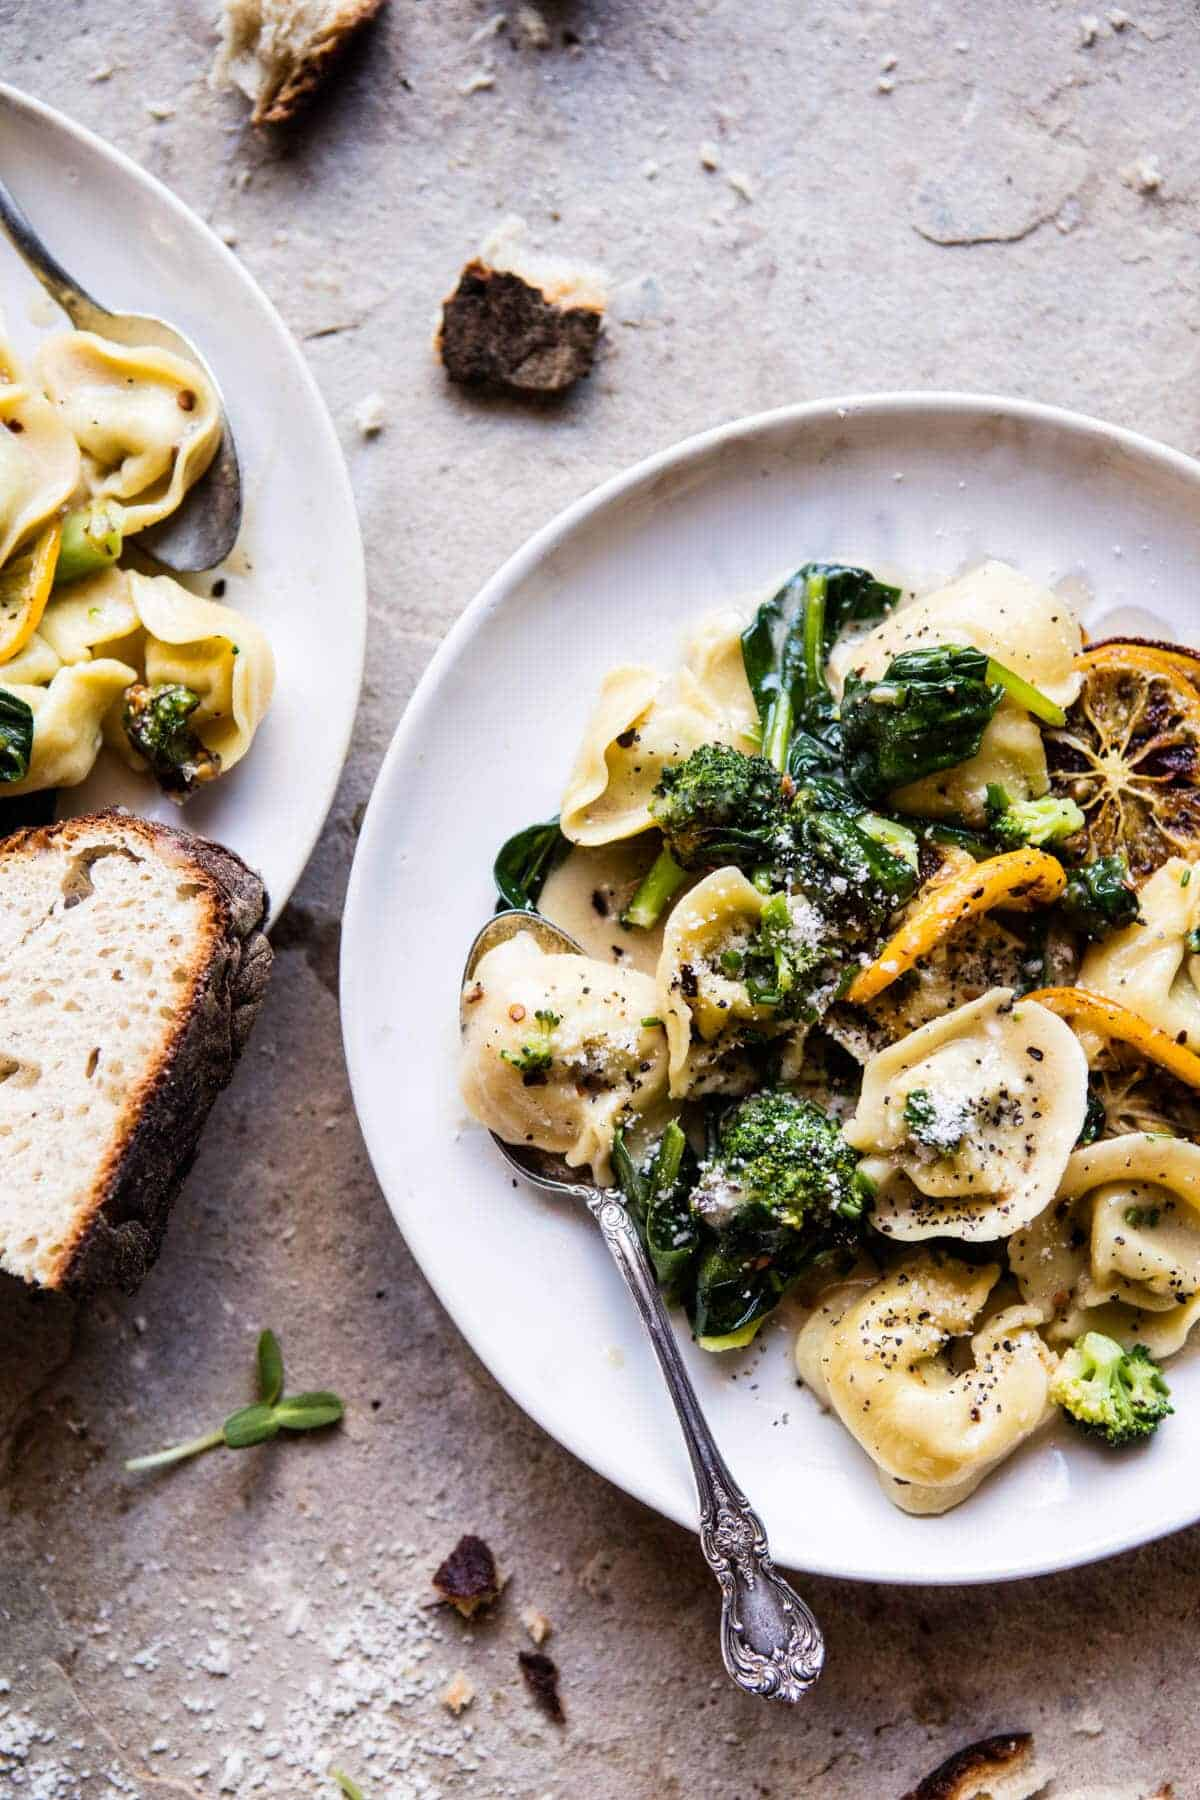
\includegraphics[width=1\textwidth,height=\textheight]{images/easy-broccoli-cheese-tortellini.jpg}

\textbf{Prep Time:} 10 min \textbar{} \textbf{Cook Time:} 10 min
\textbar{} \textbf{Total Time:} 20 min

\section{Ingredients}\label{ingredients-132}

\begin{itemize}
\tightlist
\item
  8 ounces cheese tortellini
\item
  2 heads broccoli, florets roughly chopped
\item
  2 lemons, preferably Meyer, thinly sliced
\item
  2 tablespoons olive oil
\item
  2 large handfuls baby spinach
\item
  1 tablespoon chopped fresh chives
\item
  4 tablespoons butter
\item
  1 cup grated manchego cheese
\item
  1 cup grated parmesan cheese
\item
  pinch of crushed red pepper flakes
\item
  kosher salt and pepper
\end{itemize}

\section{Instructions}\label{instructions-132}

\begin{enumerate}
\def\labelenumi{\arabic{enumi}.}
\tightlist
\item
  Bring a large pot of salted water to a boil. Add the tortellini and
  broccoli and cook according to package directions until the tortellini
  is al dente, about 4-6 minutes. During the last minute of cooking, add
  the lemon slices. Just before draining, remove 1 cup of the pasta
  cooking water. Drain. Pick out the lemon slices. Return the pot to the
  stove and set over medium heat. Add the olive oil and lemon slices.
  Fry until lightly golden on each side, about 30 seconds to 1 minute.
  Remove the pot from the heat. Add the tortellini, broccoli, spinach,
  chives, butter, cheese and a splash of the pasta cooking water. Toss
  until the cheese has melted, adding more water, little by little to
  create a loose sauce. Season with crushed red pepper, salt and pepper.
  Enjoy!
\end{enumerate}

\bookmarksetup{startatroot}

\chapter{Minty Grapefruit Caipirinha}\label{minty-grapefruit-caipirinha}

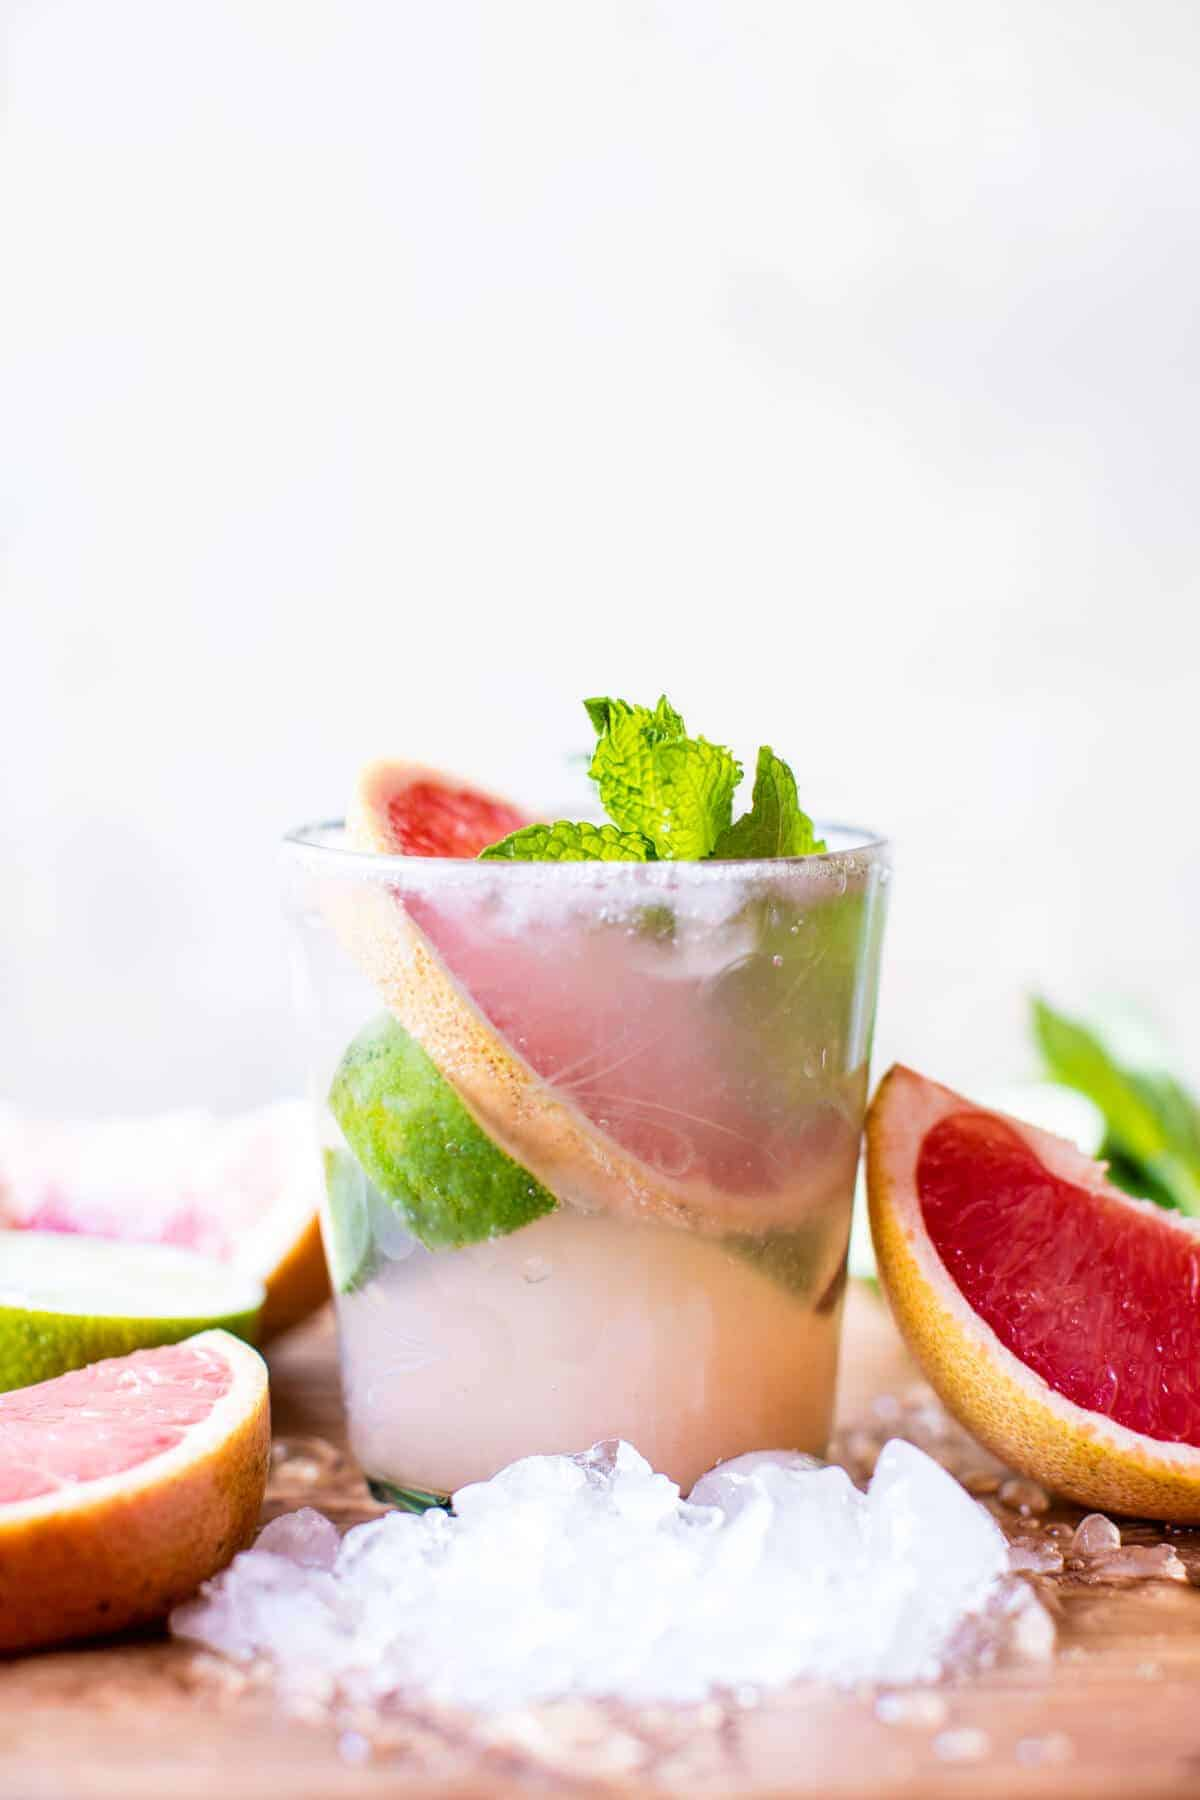
\includegraphics[width=1\textwidth,height=\textheight]{images/minty-grapefruit-caipirinha.jpg}

\textbf{Prep Time:} 5 min \textbar{} \textbf{Cook Time:} \textbar{}
\textbf{Total Time:} 5 min

\section{Ingredients}\label{ingredients-133}

\begin{itemize}
\tightlist
\item
  1-2 teaspoons honey or sugar (optional)
\item
  1 lime, quartered
\item
  6 fresh mint leaves
\item
  crushed ice
\item
  juice of 1/2 a grapefruit
\item
  2 ounces Cachaça or white rum
\item
  sparkling water, for topping
\end{itemize}

\section{Instructions}\label{instructions-133}

\begin{enumerate}
\def\labelenumi{\arabic{enumi}.}
\tightlist
\item
  In a glass, muddle 1-2 teaspoons sugar or honey (if using), the
  quartered lime and mint leaves. Add the ice, the grapefruit juice and
  the Cachaça, gently mix to combine. Pour sparkling water over top.
  DRINK! ?
\end{enumerate}

\bookmarksetup{startatroot}

\chapter{Lighter Shrimp Po Boys with Avocado Mango
Slaw}\label{lighter-shrimp-po-boys-with-avocado-mango-slaw}

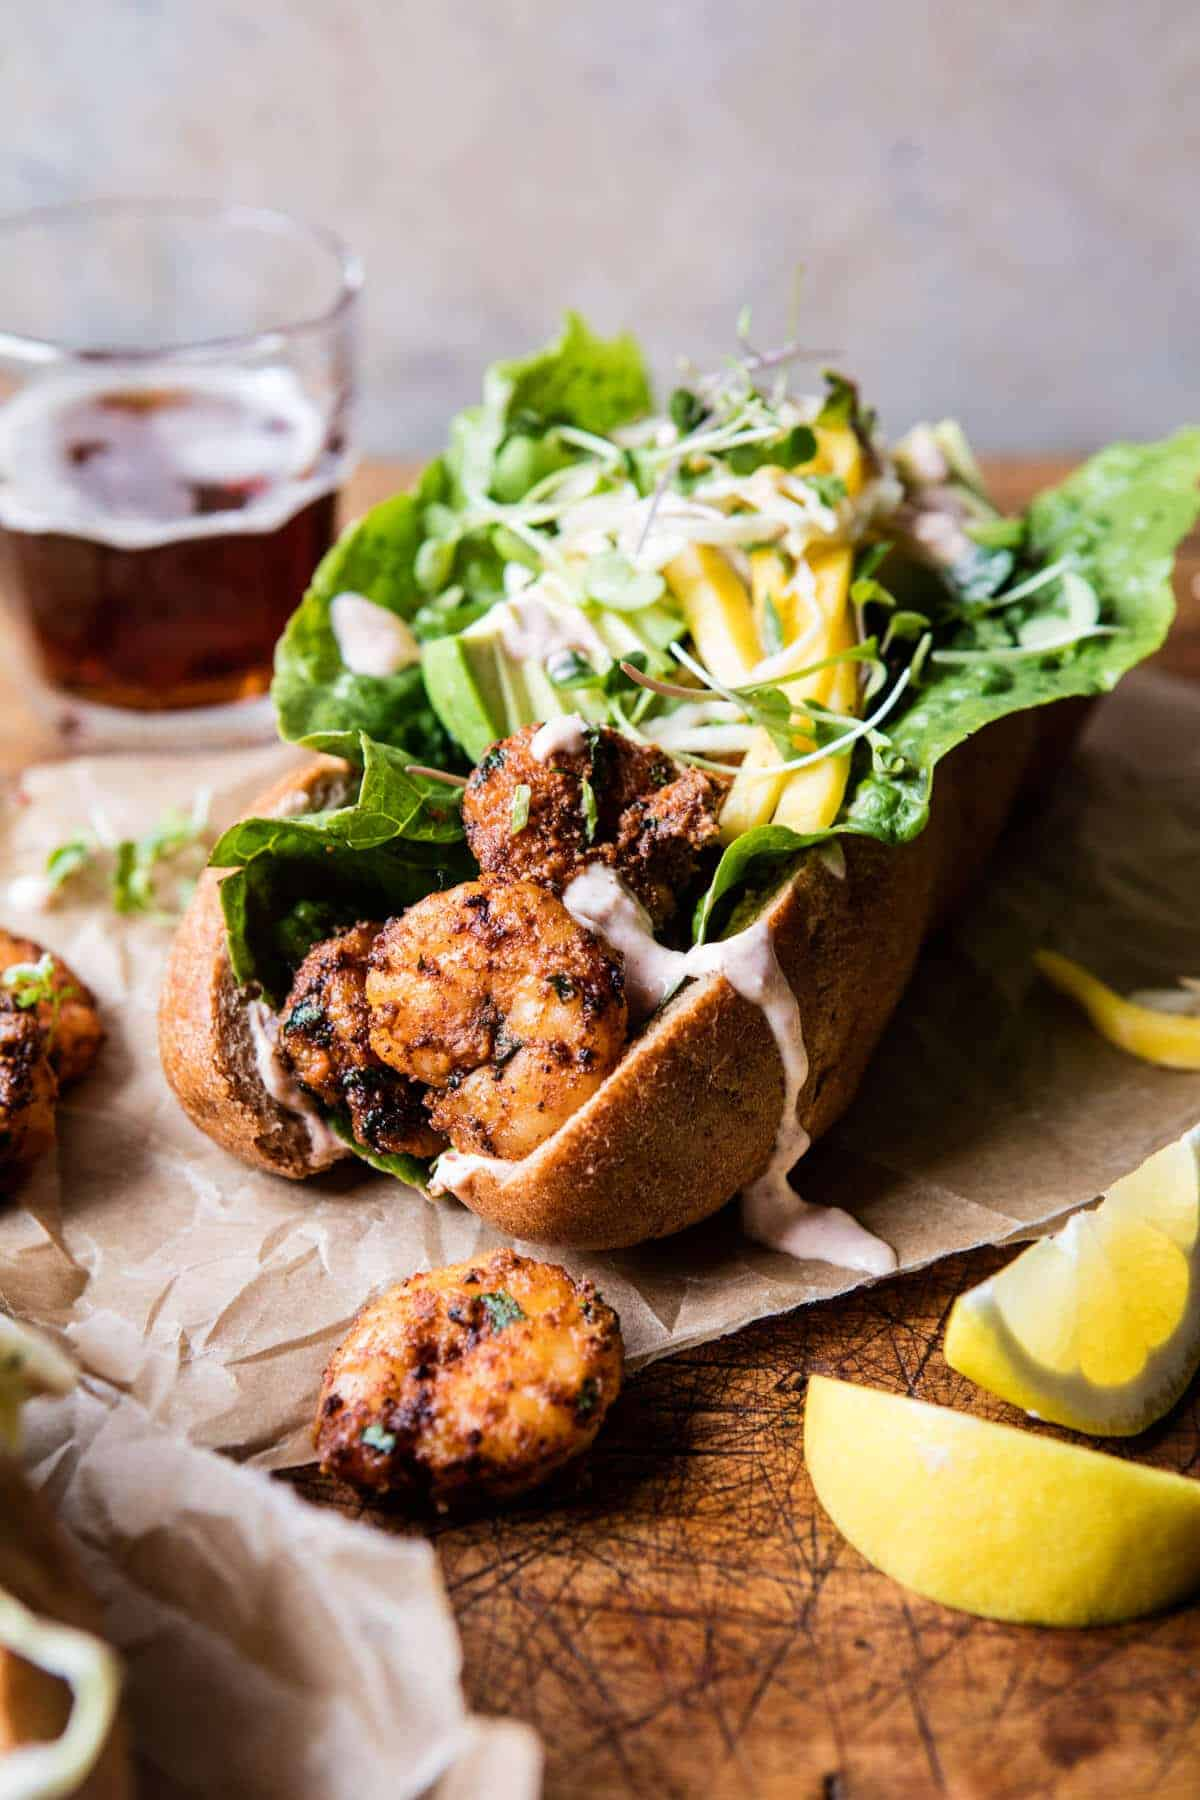
\includegraphics[width=1\textwidth,height=\textheight]{images/lighter-shrimp-po-boys-with-avocado-mango-slaw.jpg}

\textbf{Prep Time:} 20 min \textbar{} \textbf{Cook Time:} 10 min
\textbar{} \textbf{Total Time:} 30 min

\section{Ingredients}\label{ingredients-134}

\begin{itemize}
\tightlist
\item
  1 1/2 pounds shrimp, peeled
\item
  1 tablespoon creole seasoning
\item
  1 teaspoon smoked paprika
\item
  1 teaspoon cayenne pepper
\item
  1 teaspoon garlic powder
\item
  1/2 teaspoon onion powder
\item
  1/2 teaspoon dried thyme
\item
  2 tablespoons olive oil
\item
  4 whole wheat hoagie rolls
\item
  1 cup plain greek yogurt
\item
  2 tablespoons hot sauce
\item
  juice of 1 lemon
\item
  1/2 teaspoon smoked paprika
\item
  kosher salt and pepper
\item
  1/2 cup shredded cabbage
\item
  1 mango, thinly sliced into matchsticks
\item
  1 avocado, diced or sliced
\item
  1/2 cup fresh cilantro or basil (chopped)
\end{itemize}

\section{Instructions}\label{instructions-134}

\begin{enumerate}
\def\labelenumi{\arabic{enumi}.}
\tightlist
\item
  In a medium bowl, combine the shrimp, creole, paprika, cayenne, garlic
  powder, onion powder, thyme and olive oil. Let sit while you make the
  slaw or place in the fridge up to overnight.
\item
  Make the slaw. In a small bowl, combine the yogurt, hot sauce, lemon
  juice, paprika, and a pinch each of salt and pepper. Taste and adjust
  spices to your liking. In a large bowl, toss together the cabbage,
  mango, avocado, and cilantro. Add 2-3 tablespoons of the yogurt sauce,
  gently tossing to combine. Reserve the remaining yogurt for serving.
\item
  Heat a large skillet over medium high heat. Add the shrimp in a single
  layer and cook, stirring once or twice until the shrimp have turned
  pink and are cooked through.
\item
  To assemble. Divide the shrimp among the hoagie rolls and drizzle with
  yogurt sauce. Top with slaw. Enjoy!
\end{enumerate}

\bookmarksetup{startatroot}

\chapter{Singapore Sweet Potato
Noodles}\label{singapore-sweet-potato-noodles}

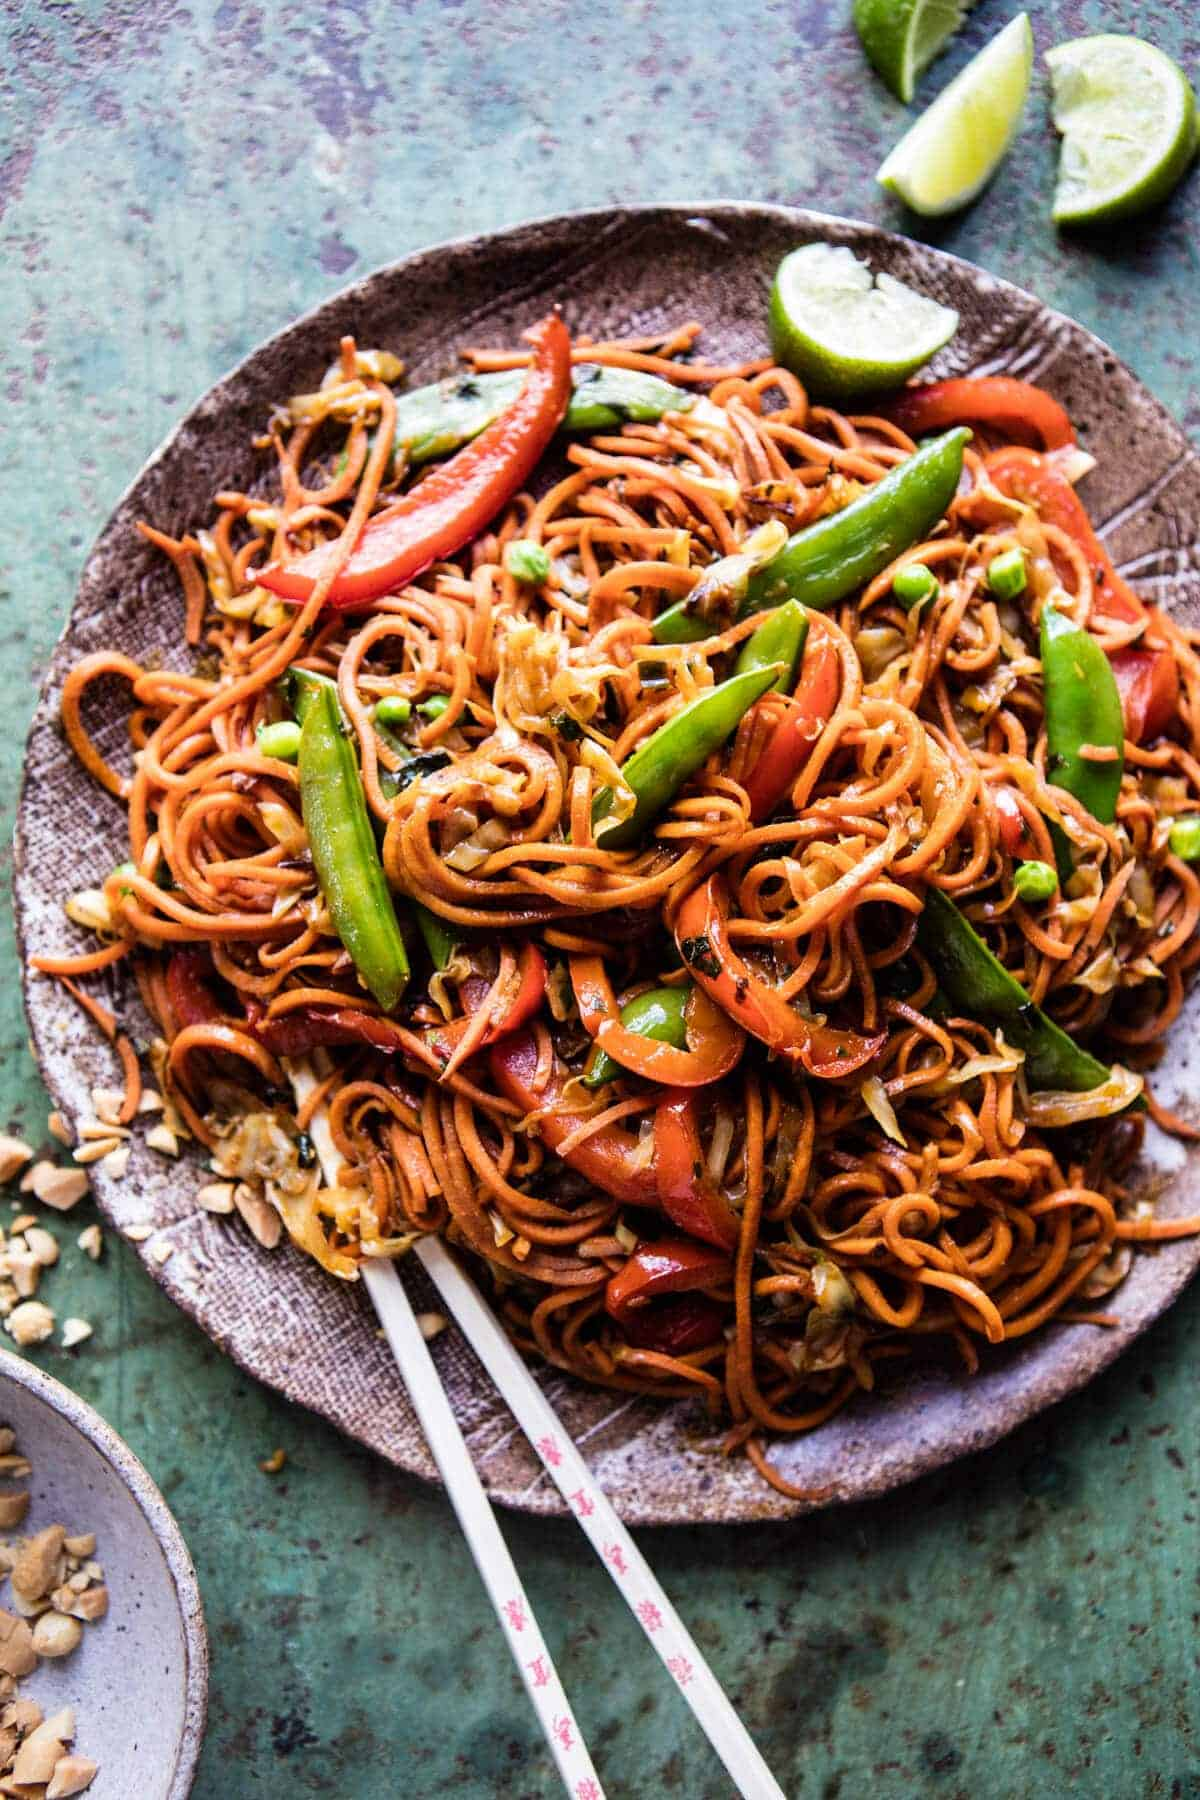
\includegraphics[width=1\textwidth,height=\textheight]{images/singapore-sweet-potato-noodles.jpg}

\textbf{Prep Time:} 15 min \textbar{} \textbf{Cook Time:} 15 min
\textbar{} \textbf{Total Time:} 30 min

\section{Ingredients}\label{ingredients-135}

\begin{itemize}
\tightlist
\item
  2 medium sweet potatoes
\item
  2 teaspoons sesame oil
\item
  1 tablespoon minced fresh ginger
\item
  1 clove garlic, minced or grated
\item
  1/4 cup tamari (or low sodium soy sauce)
\item
  1 tablespoon raw apple cider vinegar
\item
  1 tablespoon maple syrup (optional)
\item
  2-3 teaspoons curry powder
\item
  1 teaspoon coconut oil
\item
  1 red bell pepper, chopped
\item
  3 cups mung bean sprouts or shredded cabbage
\item
  6 green onions, thinly sliced
\item
  1 cup fresh or frozen peas
\item
  fresh cilantro, for garnish
\end{itemize}

\section{Instructions}\label{instructions-135}

\begin{enumerate}
\def\labelenumi{\arabic{enumi}.}
\tightlist
\item
  Using a spiralizer, turn the sweet potatoes into spaghetti-like
  noodles or use a vegetable peeler to create long, thin, ribbons, then
  set them aside. To prepare the sauce. in a small bowl, whisk together
  the sesame oil, ginger, garlic, tamari, vinegar, maple syrup, and 2
  teaspoons of the curry powder, then set aside. In a large Dutch oven,
  melt the coconut oil over medium heat and cook the bell pepper until
  it starts to soften, about 5 minutes. Add the bean sprouts and
  reserved sauce and cook until the vegetables shrink in size, about 5
  minutes more. Add the sweet potato noodles, green onions, and peas and
  toss well to combine. Partially cover the pot and cook until the
  potatoes are tender, 8 to 10 minutes.Taste and adjust the seasonings,
  adding more curry powder if desired. Serve warm, garnished with
  cilantro. Store leftovers in an airtight container in the refrigerator
  for up to 3 days.
\end{enumerate}

\bookmarksetup{startatroot}

\chapter{Cuban Style Steak and Avocado Rice with Pineapple
Chimichurri}\label{cuban-style-steak-and-avocado-rice-with-pineapple-chimichurri}

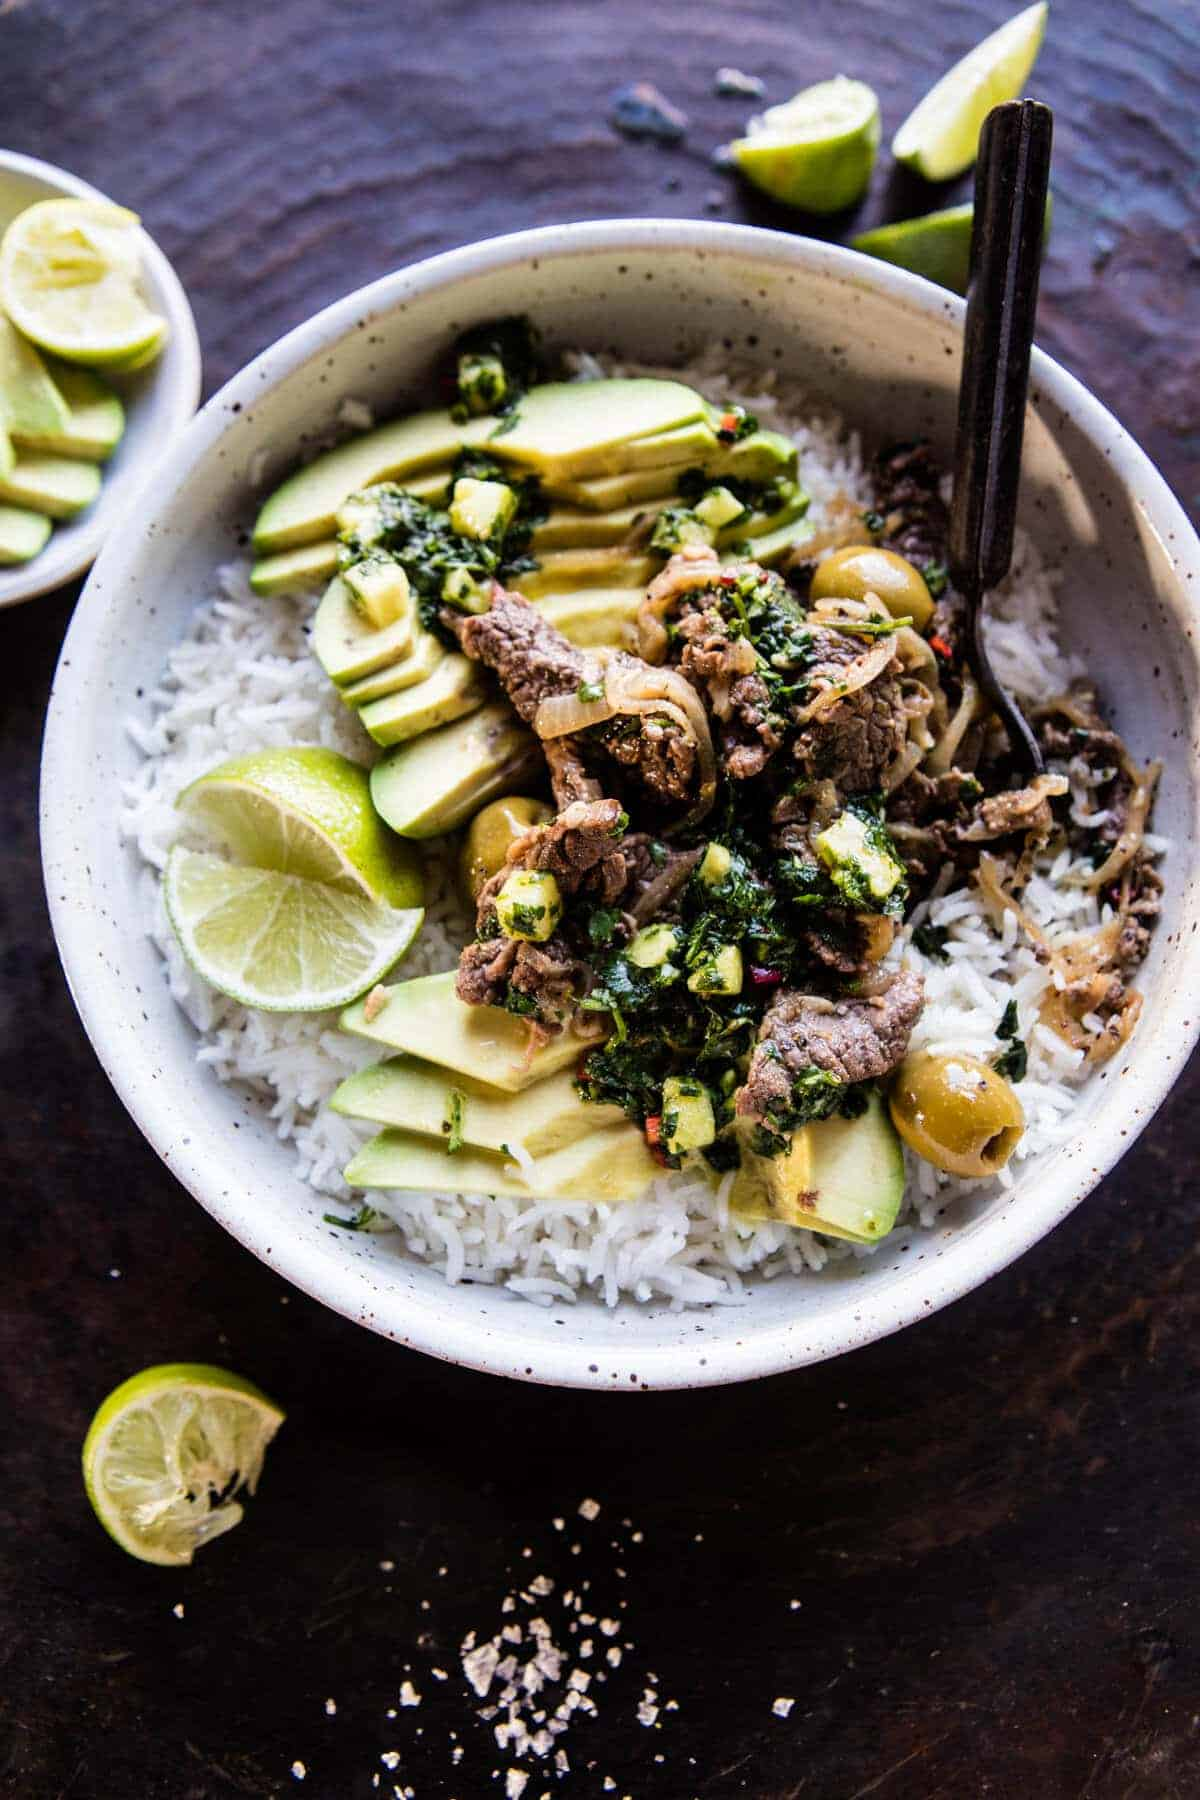
\includegraphics[width=1\textwidth,height=\textheight]{images/cuban-style-steak-and-avocado-rice-with-pineapple-chimichurri.jpg}

\textbf{Prep Time:} 15 min \textbar{} \textbf{Cook Time:} 15 min
\textbar{} \textbf{Total Time:} 1 hr

\section{Ingredients}\label{ingredients-136}

\begin{itemize}
\tightlist
\item
  1 1/4 cups fresh cilantro, chopped
\item
  1 cup diced pineapple
\item
  1 Fresno chile pepper, seeded + chopped
\item
  1 clove garlic, minced or grated
\item
  1/4 cup red wine vinegar
\item
  1/4 cup olive oil
\item
  juice of 1 lime
\item
  kosher salt and pepper
\item
  2 pounds skirt steak, thinly sliced
\item
  1/4 cup olive oil
\item
  8 cloves garlic, minced or grated
\item
  1/4 cup fresh oregano, chopped
\item
  2 teaspoons cumin
\item
  2 dried bay leaves
\item
  juice from 2 limes
\item
  1 teaspoon kosher salt and pepper
\item
  2 sweet onions, thinly sliced
\item
  1/2 cup green olives
\item
  1 avocado, sliced
\item
  steamed riced, for serving
\end{itemize}

\section{Instructions}\label{instructions-136}

\begin{enumerate}
\def\labelenumi{\arabic{enumi}.}
\tightlist
\item
\end{enumerate}

\bookmarksetup{startatroot}

\chapter{Mediterranean Roasted Red Pepper
Pizza}\label{mediterranean-roasted-red-pepper-pizza}

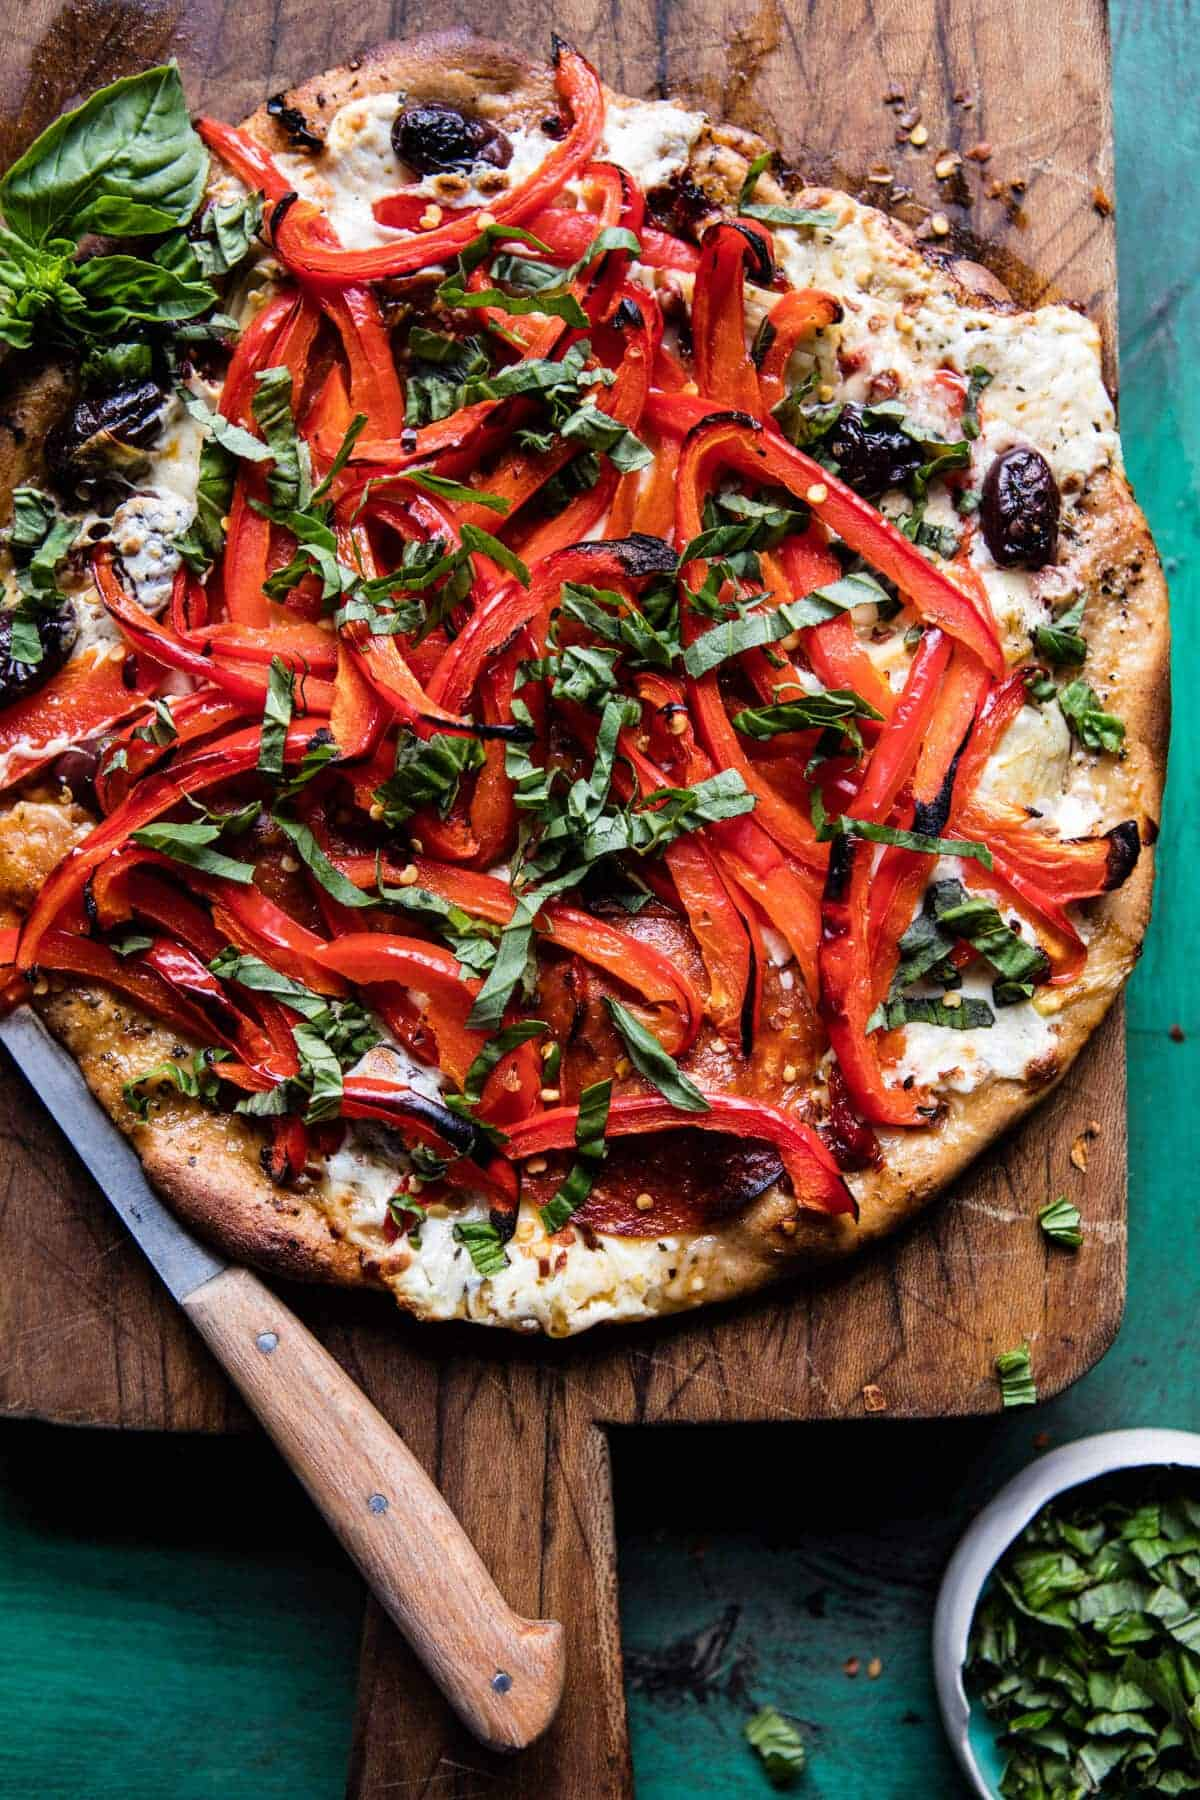
\includegraphics[width=1\textwidth,height=\textheight]{images/mediterranean-roasted-red-pepper-pizza.jpg}

\textbf{Prep Time:} 15 min \textbar{} \textbf{Cook Time:} 15 min
\textbar{} \textbf{Total Time:} 30 min

\section{Ingredients}\label{ingredients-137}

\begin{itemize}
\tightlist
\item
  1/2 pound pizza dough
\item
  2 tablespoons olive oil
\item
  2 garlic, minced or grated
\item
  1 teaspoon dried basil
\item
  1 teaspoon dried oregano
\item
  1/2 teaspoon crushed red pepper flakes
\item
  kosher salt and pepper
\item
  1/2 cup pitted kalamata olives
\item
  1/3 cup oil packed sun-dried tomatoes, oil drained and sliced
\item
  1/4 cup marinated artichokes, drained
\item
  8 ounces mozzarella, torn or shredded
\item
  1/2 cup shredded fontina cheese
\item
  4-8 pepperoni slices (optional)
\item
  2 red bell peppers, very thinly sliced
\item
  fresh basil, for topping
\end{itemize}

\section{Instructions}\label{instructions-137}

\begin{enumerate}
\def\labelenumi{\arabic{enumi}.}
\tightlist
\item
  Preheat oven to 425 degrees F. Grease a baking sheet with olive oil.On
  a lightly floured surface, push/roll the dough out until it is very
  thin. For SUPER thin pizza, divide the dough into two and roll out.
  Transfer the dough to the prepared baking sheet. Spread the dough with
  olive oil. Add the garlic, basil, oregano, crushed red pepper flakes,
  and a pinch each of salt and pepper. Spread evenly over the dough. Add
  the olives, sun-dried tomatoes, artichokes, and cheese. Top with
  pepperoni and bell peppers. Transfer to the oven and bake 10-15
  minutes or until the crust is crisp and the cheese has melted. Remove
  the pizza from the oven and top with basil. EAT!
\end{enumerate}

\bookmarksetup{startatroot}

\chapter{Raspberry Rose Tequila
Kombucha.}\label{raspberry-rose-tequila-kombucha.}

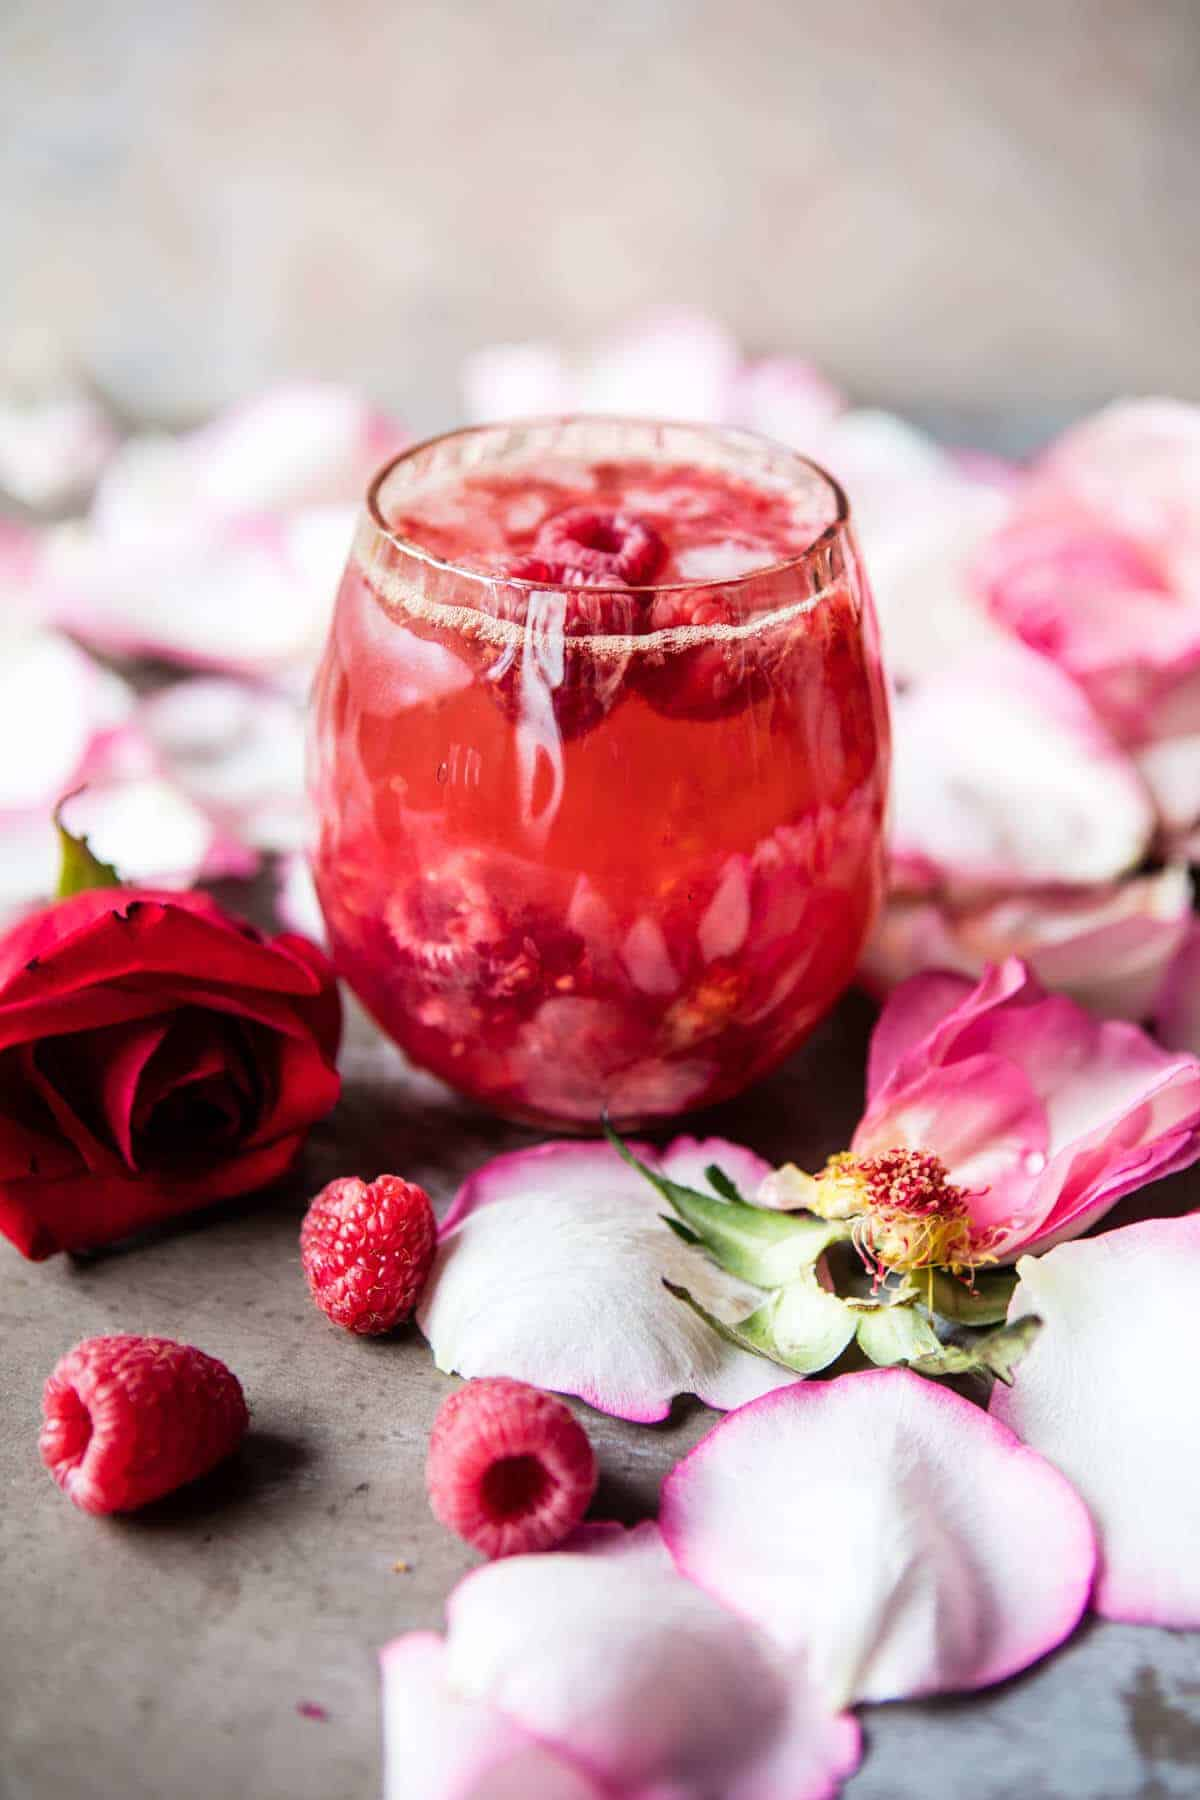
\includegraphics[width=1\textwidth,height=\textheight]{images/raspberry-rose-tequila-kombucha-.jpg}

\textbf{Prep Time:} 5 min \textbar{} \textbf{Cook Time:} \textbar{}
\textbf{Total Time:} 5 min

\section{Ingredients}\label{ingredients-138}

\begin{itemize}
\tightlist
\item
  4 fresh or frozen raspberries
\item
  juice of 1/2 a lemon
\item
  2 ounces silver tequila
\item
  1-2 teaspoons rose water (optional)
\item
  1 plain or ginger kombucha
\end{itemize}

\section{Instructions}\label{instructions-138}

\begin{enumerate}
\def\labelenumi{\arabic{enumi}.}
\tightlist
\item
  Muddle the raspberries, lemon juice, tequila, and rose water in a
  glass. Add ice, gently mix to combine. Pour the kombucha over top,
  again gently stirring to combine. DRINK! ?
\end{enumerate}

\bookmarksetup{startatroot}

\chapter{Soft and Fluffy Cream Cheese Sugar
Cookies.}\label{soft-and-fluffy-cream-cheese-sugar-cookies.}


\includegraphics[width=1\textwidth,height=\textheight]{images/soft-and-fluffy-cream-cheese-sugar-cookies-.jpg}

\textbf{Prep Time:} 25 min \textbar{} \textbf{Cook Time:} 10 min
\textbar{} \textbf{Total Time:} 55 min

\section{Ingredients}\label{ingredients-139}

\begin{itemize}
\tightlist
\item
  3/4 cup (1 1/2 sticks) unsalted butter, at room temperature
\item
  4 ounces cream cheese, at room temperature
\item
  3/4 cups granulated sugar
\item
  1 teaspoon vanilla extract
\item
  1 egg, at room temperature*
\item
  2 1/4- 2 1/2 cups all purpose flour
\item
  1/2 teaspoon baking soda
\item
  1/4 teaspoon salt
\item
  2 cups powdered sugar
\item
  1 tablespoons meringue powder (optional)
\item
  3-6 tablespoons water
\item
  1/2 vanilla bean, seeds removed or 1 teaspoon vanilla extract
\item
  beet juice or food coloring
\end{itemize}

\section{Instructions}\label{instructions-139}

\begin{enumerate}
\def\labelenumi{\arabic{enumi}.}
\tightlist
\item
  In a large mixing bowl, cream together the butter, cream cheese,
  sugar, and vanilla until light and fluffy, about a full 3-5 minutes.
  Add the egg and mix until evenly combined. Add the 2 1/4 cups flour,
  baking soda and salt, beating until combined and the dough forms a
  ball, adding more flour if needed.Generously flour your work surface.
  Divide the dough in half and flatten each half into a disk. Roll out
  the dough to 1/4 inch thickness. Make sure you are using enough flour
  or your dough will stick. Cut out the cookies into your desired
  shapes. Carefully transfer the cookies to a parchment lined baking
  sheet. Cover the baking sheet and place the sheet in the freezer,
  freeze until very firm, about 20-15 minutes. Roll out the leftover
  scraps, and repeat with the remaining disk of dough.Preheat oven to
  350 degrees. Bake the cookies on the middle rack of the oven for 12-15
  minutes or until just lightly golden brown. Do not over bake. Cool on
  the baking sheet five minutes and then transfer to a wire cooling rack
  to cool completely.To make the icing, combine the sugar, meringue
  powder and 3 tablespoons water. Mix until icing holds a ribbonlike
  trail on the surface. Add the vanilla and 1-3 teaspoons beet juice and
  mix until just combined.Frost the cooled cookies and decorate as
  desired. Keep stored in an airtight container for up to 5 days.
\end{enumerate}

\bookmarksetup{startatroot}

\chapter{Greek Goddess Chicken Lettuce
Wraps.}\label{greek-goddess-chicken-lettuce-wraps.}

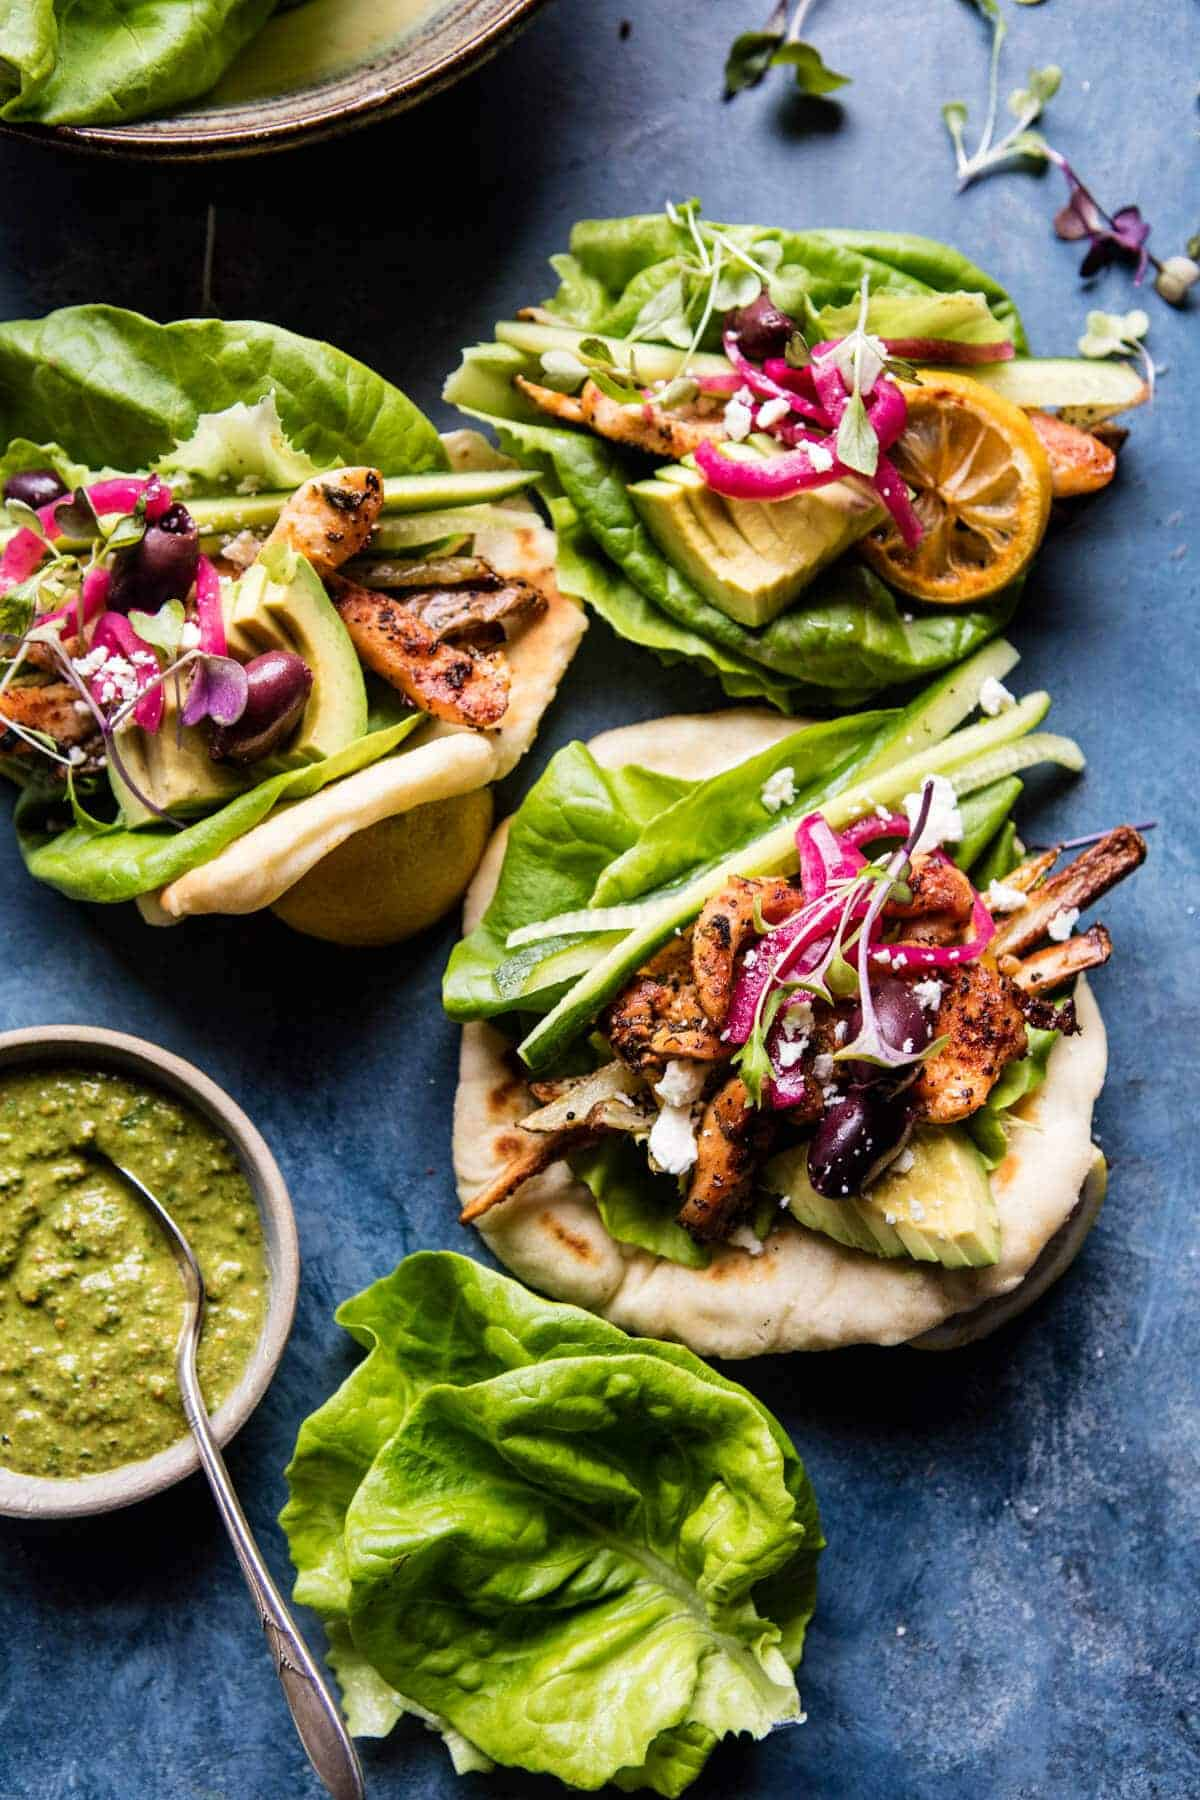
\includegraphics[width=1\textwidth,height=\textheight]{images/greek-goddess-chicken-lettuce-wraps-.jpg}

\textbf{Prep Time:} 20 min \textbar{} \textbf{Cook Time:} 25 min
\textbar{} \textbf{Total Time:} 45 min

\section{Ingredients}\label{ingredients-140}

\begin{itemize}
\tightlist
\item
  4 tablespoons olive oil
\item
  1 pound boneless, skinless chicken, cut into strips
\item
  2 cloves garlic, minced or grated
\item
  1 tablespoon smoked paprika
\item
  1/4 cup fresh oregano, chopped
\item
  1 lemon, sliced
\item
  kosher salt and pepper
\item
  2 potatoes, cut into matchsticks
\item
  4 warmed pitas (optional)
\item
  1 head butter lettuce
\item
  2 Persian cucumbers, cut into matchsticks
\item
  1 avocado, sliced
\item
  1/3 cup kalamata olives, pitted
\item
  feta cheese, pickled red onion and microgreens, for serving
\item
  1/2 cup roasted pistachios
\item
  2 tablespoons lemon juice
\item
  1 clove garlic
\item
  1 cup fresh basil
\item
  1 jalapeno, halved (seed if desired)
\item
  kosher salt
\end{itemize}

\section{Instructions}\label{instructions-140}

\begin{enumerate}
\def\labelenumi{\arabic{enumi}.}
\tightlist
\item
  In a large ziplock back, combine 2 tablespoons olive oil, the chicken,
  garlic, smoked paprika, oregano, lemon and a large pinch of both salt
  and pepper. Marinate in the fridge for 30 minutes or up to
  overnight.Preheat the oven to 425 degrees F.Dump the chicken out into
  a 9x13 inch baking dish. Transfer to the oven and roast for 20-25
  minutes or until the chicken is cooked through.During the same time,
  toss together the remaining 2 tablespoons olive oil, potatoes and a
  pinch each of salt and pepper. Transfer the potatoes to the oven and
  bake for 20-30 minutes, tossing halfway through cooking until golden
  crisp.To assemble, layer the lettuce inside a warm pita. Add the fries
  and chicken. Top with cucumber, avocado, olives, feta, onion, and
  greens. Serve drizzled generously with Goddess Sauce (below).
\end{enumerate}

\bookmarksetup{startatroot}

\chapter{Valentine's Surprise Chocolate High Hat
Cupcakes}\label{valentines-surprise-chocolate-high-hat-cupcakes}

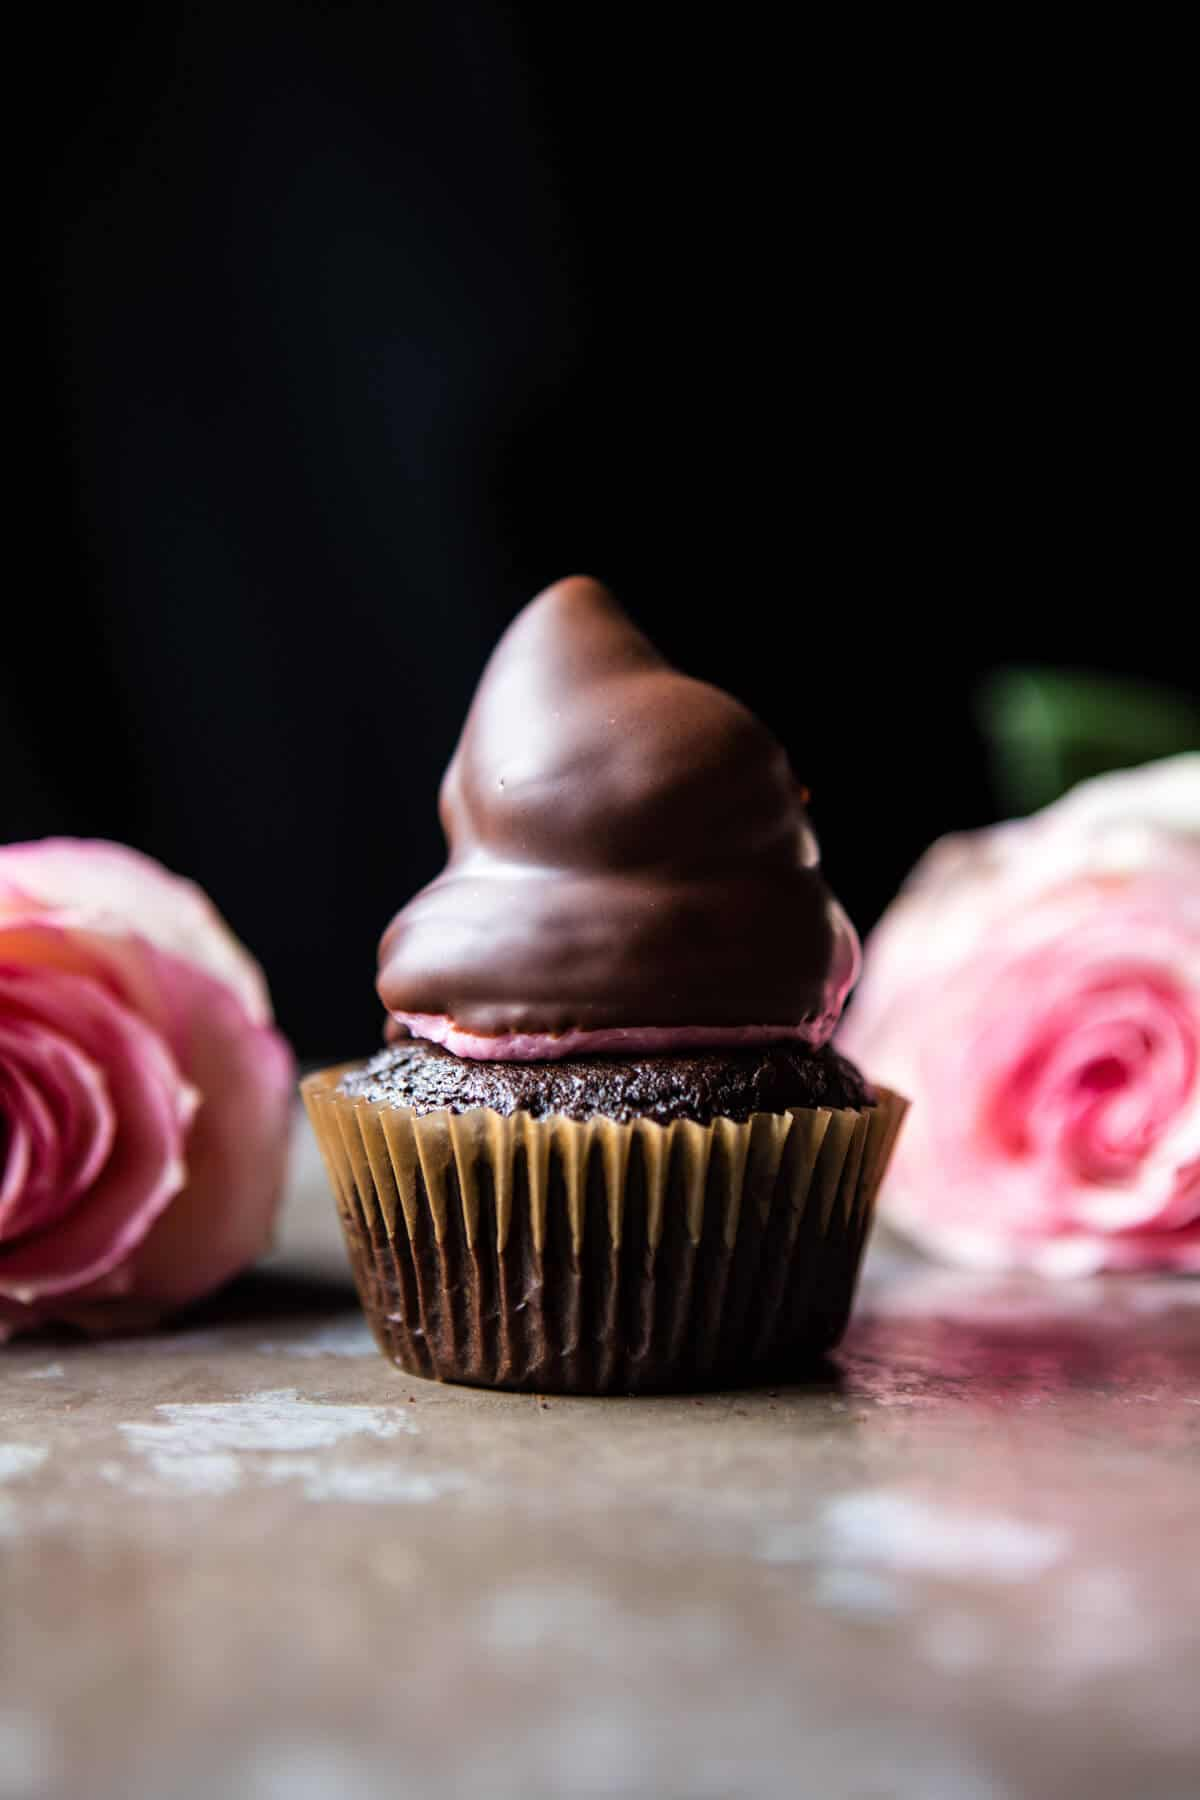
\includegraphics[width=1\textwidth,height=\textheight]{images/valentine-s-surprise-chocolate-high-hat-cupcakes.jpg}

\textbf{Prep Time:} 30 min \textbar{} \textbf{Cook Time:} 30 min
\textbar{} \textbf{Total Time:} 1 hr

\section{Ingredients}\label{ingredients-141}

\begin{itemize}
\tightlist
\item
  1 1/2 cups all-purpose flour
\item
  1 1/2 cups granulated sugar
\item
  1 cup unsweetened cocoa powder
\item
  1 1/2 teaspoons baking soda
\item
  1 1/2 teaspoons baking powder
\item
  1 teaspoon salt
\item
  2 eggs (at room temperature*)
\item
  1 cup buttermilk
\item
  1/2 cup canola oil
\item
  1 tablespoon vanilla extract
\item
  1/2 cup hot brewed coffee (or water)
\item
  1/2 cup Nutella
\item
  3 eggs whites
\item
  3/4 cup granulated sugar
\item
  1 1/2 sticks (3/4 cup) unsalted butter (softened)
\item
  1 teaspoon vanilla extract
\item
  1-2 teaspoons beet juice or 1-2 drops red food coloring
\item
  2 cups semi-sweet chocolate chips
\item
  3 tablespoons coconut oil or canola oil
\end{itemize}

\section{Instructions}\label{instructions-141}

\begin{enumerate}
\def\labelenumi{\arabic{enumi}.}
\tightlist
\item
  Preheat the oven to 350 degrees F. Line 2 cupcake tins with paper
  liners.
\item
  In a medium bowl combine the flour, sugar, unsweetened cocoa powder,
  baking soda, baking powder and salt.
\item
  In the bowl of a stand mixer (or use a hand held mixer) beat together
  the eggs, buttermilk, canola oil and vanilla until smooth. Slowly add
  the dry ingredients to the wet ingredients with the mixer on low until
  there are no longer any clumps of flour. Add the coffee and mix until
  combined. Batter should be pourable, but not super thin.
\item
  Pour the batter among 18-20 cupcake liners. Transfer to the oven and
  bake for 12-15 minutes, until the tops are just set and no longer
  wiggly in the center. Remove and let cool completely before filling
  and frosting.
\item
  Use a small paring knife to cut a cone-shaped piece from the center of
  each cooled cupcake. Fill the hole with nutella, then replace the top
  portion of the cone (you'll need to slice off the tip).
\item
  To make the buttercream. Bring a large pot (big enough to place your
  mixing bowl over top) of water to boil. In the bowl of a stand mixer
  whisk the egg whites and sugar together. Place the bowl of the stand
  mixer over the pot of boiling water and cook, stirring often, until
  the egg whites are very warm to the touch and the sugar has dissolved,
  remove the bowl from the heat. Whip the egg whites on high until stiff
  peaks form. Allow the egg whites to cool before continuing. Once cool,
  add the butter, vanilla and beet juice/food coloring. Beat until
  combined and fluffy.
\item
  Transfer to a pastry bag fitted with a round tip. Pipe frosting into a
  swirl on each cupcake. Place the cupcakes in the fridge, covered for
  at least an hour to chill or up to overnight.
\item
  To make the chocolate coating. In a microwave safe bowl, microwave the
  chocolate chips and oil, stirring every 30 seconds until melted and
  smooth. Let the coating sit 10-15 minutes before dipping the cupcakes.
  Dip each cupcake in the chocolate, allowing any excess to drip off.
  Allow the chocolate to harden and then either serve or store covered
  in a cool and dark place for up to 3-4 days.
\end{enumerate}

\bookmarksetup{startatroot}

\chapter{Glowing Citrus, Avocado, Quinoa, and Blackened Salmon
Salad.}\label{glowing-citrus-avocado-quinoa-and-blackened-salmon-salad.}

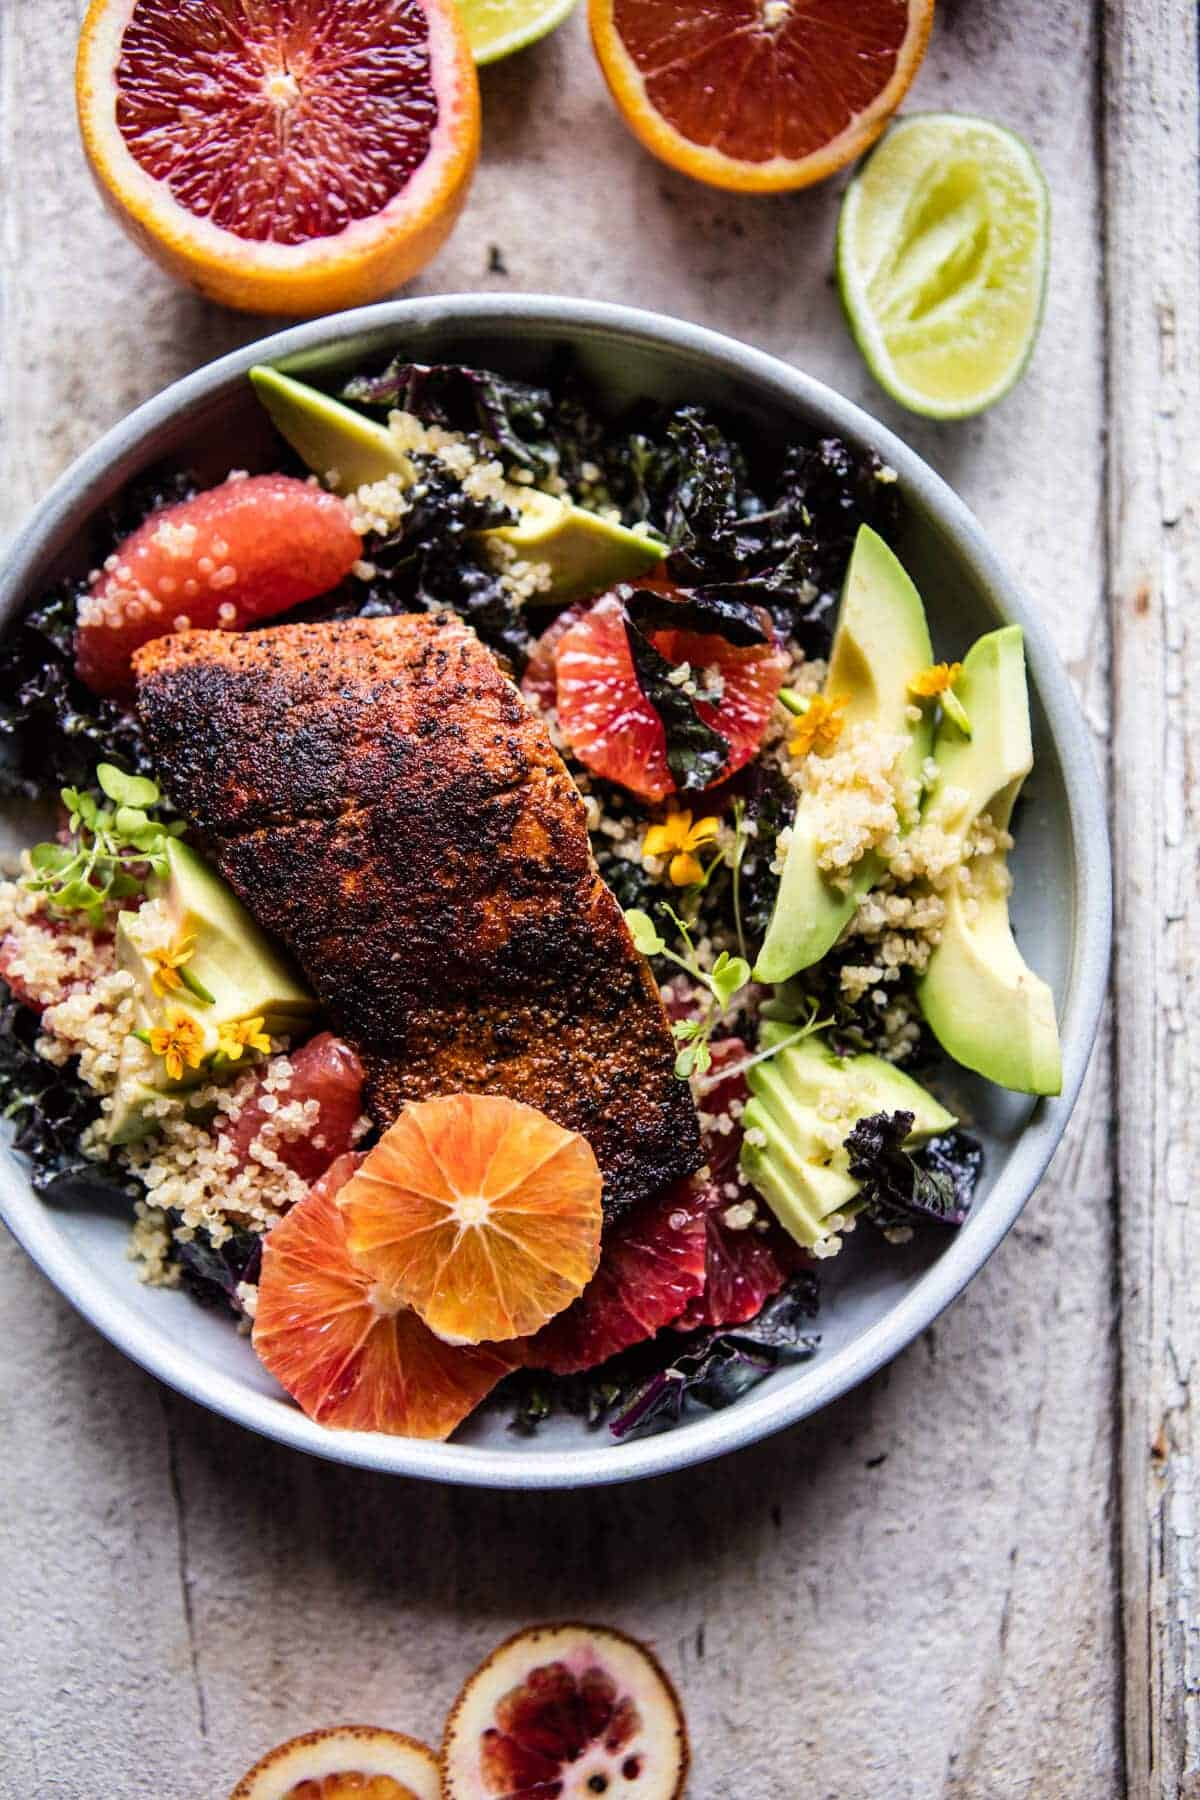
\includegraphics[width=1\textwidth,height=\textheight]{images/glowing-citrus-avocado-quinoa-and-blackened-salmon-salad-.jpg}

\textbf{Prep Time:} 20 min \textbar{} \textbf{Cook Time:} 10 min
\textbar{} \textbf{Total Time:} 30 min

\section{Ingredients}\label{ingredients-142}

\begin{itemize}
\tightlist
\item
  1 pound skin on salmon (cut into 4 pieces)
\item
  2 tablespoons olive oil
\item
  1 tablespoon smoked paprika
\item
  1/2 teaspoon garlic powder
\item
  1/2 teaspoon dried thyme
\item
  1/2 teaspoon kosher salt and pepper
\item
  zest of 1 lime
\item
  1 cup plain greek yogurt
\item
  1/2 cup fresh cilantro
\item
  juice of 2 limes
\item
  1 teaspoon honey
\item
  kosher salt
\item
  1 bunch kale (chopped)
\item
  3 oranges or grapefruits (I used grapefruit, blood and cara cara
  oranges)
\item
  1 avocado (sliced)
\item
  1 cup cooked quinoa
\item
  fresh cilantro (microgreens, and or basil, for topping)
\end{itemize}

\section{Instructions}\label{instructions-142}

\begin{enumerate}
\def\labelenumi{\arabic{enumi}.}
\tightlist
\item
  In a large gallon size zip-top bag or bowl, combine the olive oil,
  smoked paprika, garlic powder, thyme, salt, pepper and lime zest +
  lime juice. Add the salmon and toss to combine.
\item
  Heat a medium size skillet over medium-high heat. Add the salmon, skin
  side facing up. Sear the salmon for 3-4 minutes and then flip and
  continue cooking for another 4-5 minutes or until the salmon reaches
  your desired doneness. Cooking times will vary depending on the size
  of your salmon.
\item
  To make the salad. In a blender, combine the yogurt, cilantro, lime
  juice, honey and a large pinch of salt. Blend until creamy and smooth.
  Taste and add salt if needed.
\item
  Add the kale to a large bowl and massage with a few tablespoons of the
  yogurt sauce. Add the oranges, avocado, and quinoa and gently toss to
  combine. Divide the salad among plates and top with salmon. Serve with
  the remaining yogurt sauce.
\end{enumerate}

\bookmarksetup{startatroot}

\chapter{Chicken Parmesan Meatball
Crostini.}\label{chicken-parmesan-meatball-crostini.}

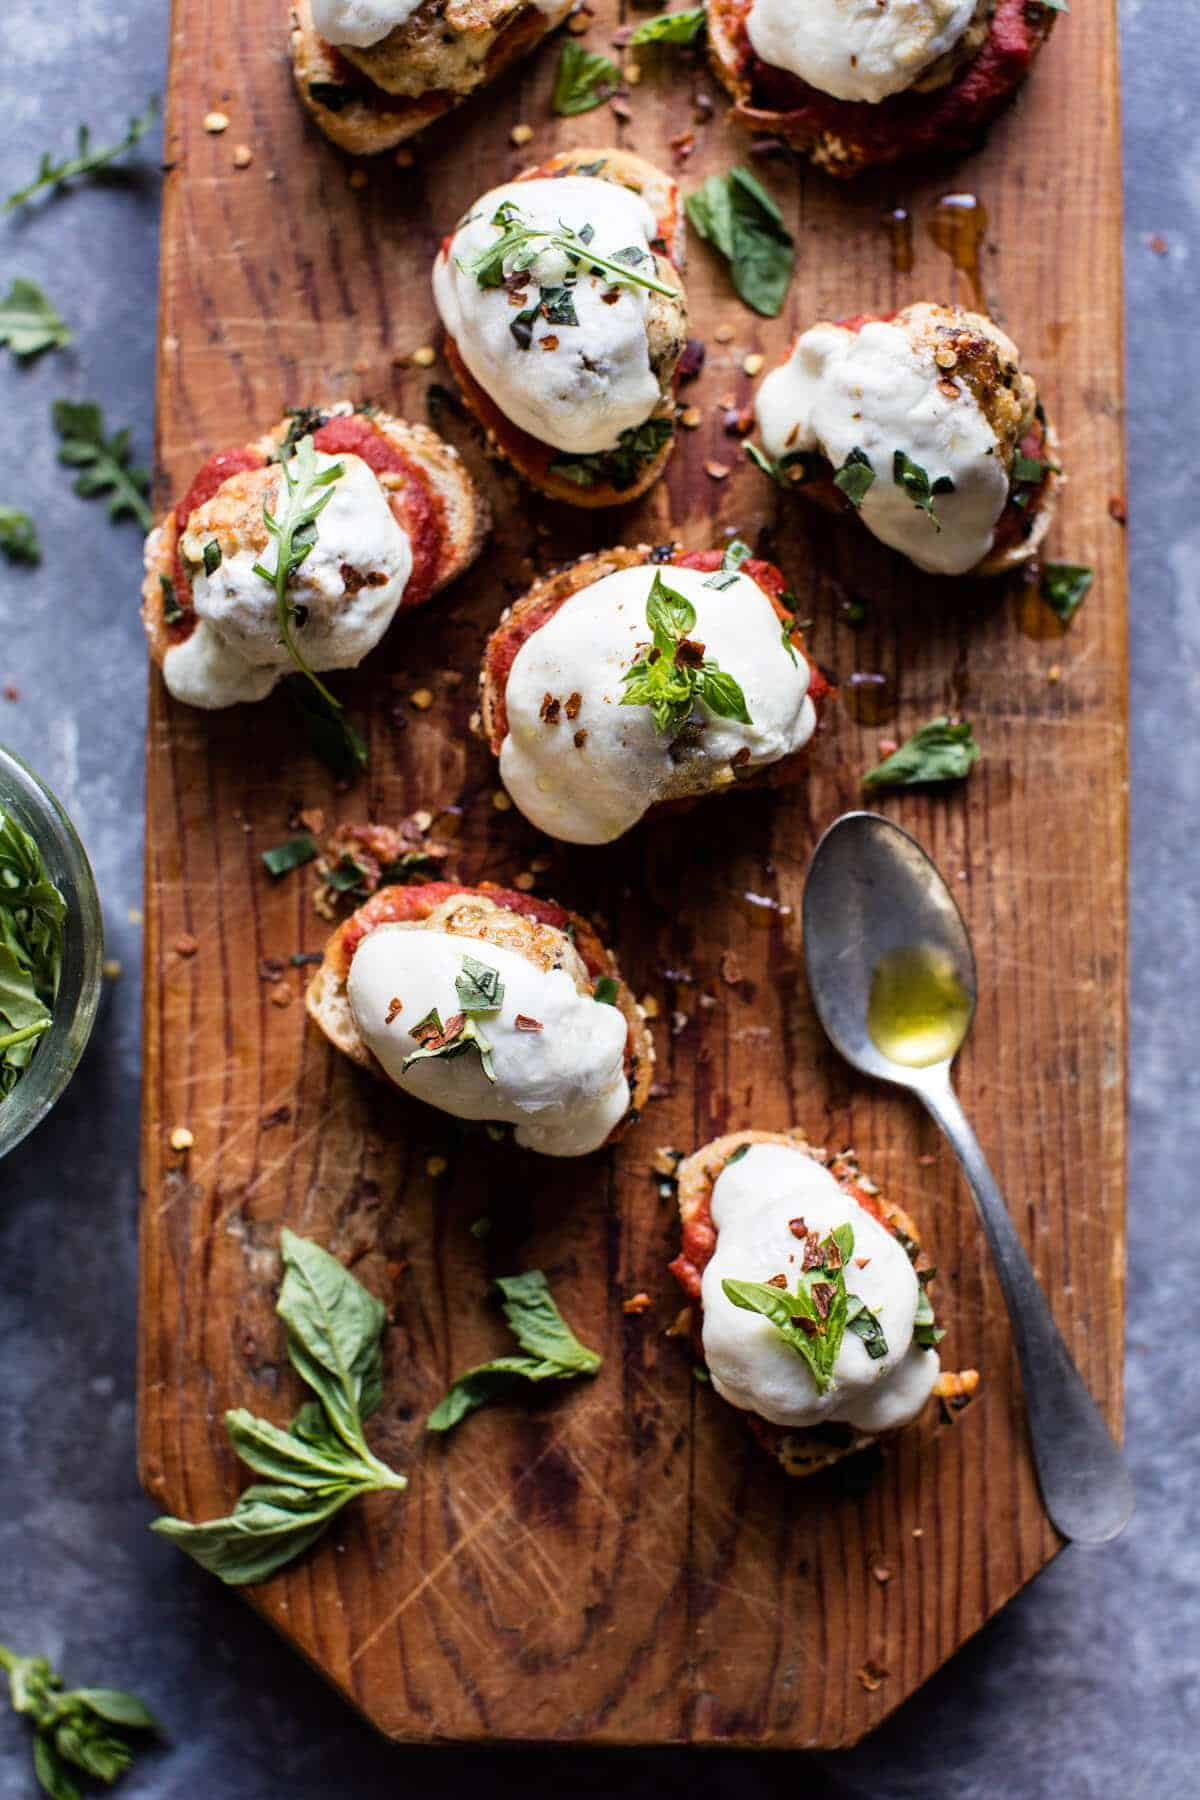
\includegraphics[width=1\textwidth,height=\textheight]{images/chicken-parmesan-meatball-crostini-.jpg}

\textbf{Prep Time:} 10 min \textbar{} \textbf{Cook Time:} 20 min
\textbar{} \textbf{Total Time:} 30 min

\section{Ingredients}\label{ingredients-143}

\begin{itemize}
\tightlist
\item
  1 pound ground chicken
\item
  1/4 cup panko bread crumbs
\item
  1/4 cup grated pecorino or parmesan cheese
\item
  1 egg
\item
  2 teaspoons Italian seasoning
\item
  kosher salt and pepper
\item
  1 loaf whole grain french bread (sliced)
\item
  3 tablespoons olive oil
\item
  1/2 cup fresh basil (chopped)
\item
  1 cup marinara sauce
\item
  8 ounces mozzarella cheese
\item
  fresh basil and or arugula (for serving)
\end{itemize}

\section{Instructions}\label{instructions-143}

\begin{enumerate}
\def\labelenumi{\arabic{enumi}.}
\tightlist
\item
  In a medium bowl, combine the ground chicken, bread crumbs, pecorino,
  egg, Italian seasoning and a pinch each of salt and pepper.
\item
  Roll mixture into scant tablespoon size balls, you should get around
  16 meatballs.
\item
  Preheat the oven to 375 degrees F.
\item
  Arrange the bread slices on a baking sheet and drizzle lightly with
  olive oil to coat. Sprinkle the fresh basil over the bread. Transfer
  to the oven and bake for 8-10 minutes or until toasted.
\item
  Meanwhile, heat a large skillet over medium heat and add a tablespoon
  of olive oil. When the oil shimmers, add the meatballs and cook for
  3-5 minutes per side or until lightly golden, about 8-10 minutes
  total.
\item
  Remove the bread from the oven and top each piece with a little
  marinara. Add a meatball and then top with mozzarella. Return the
  baking sheet to the oven and bake for 5-10 minutes or until the cheese
  has melted.
\item
  Serve the crostini warm, topped with fresh basil and extra parmesan.
\end{enumerate}

\bookmarksetup{startatroot}

\chapter{Buffalo Cheddar Soft Pretzel Twists with Everything
Spice.}\label{buffalo-cheddar-soft-pretzel-twists-with-everything-spice.}

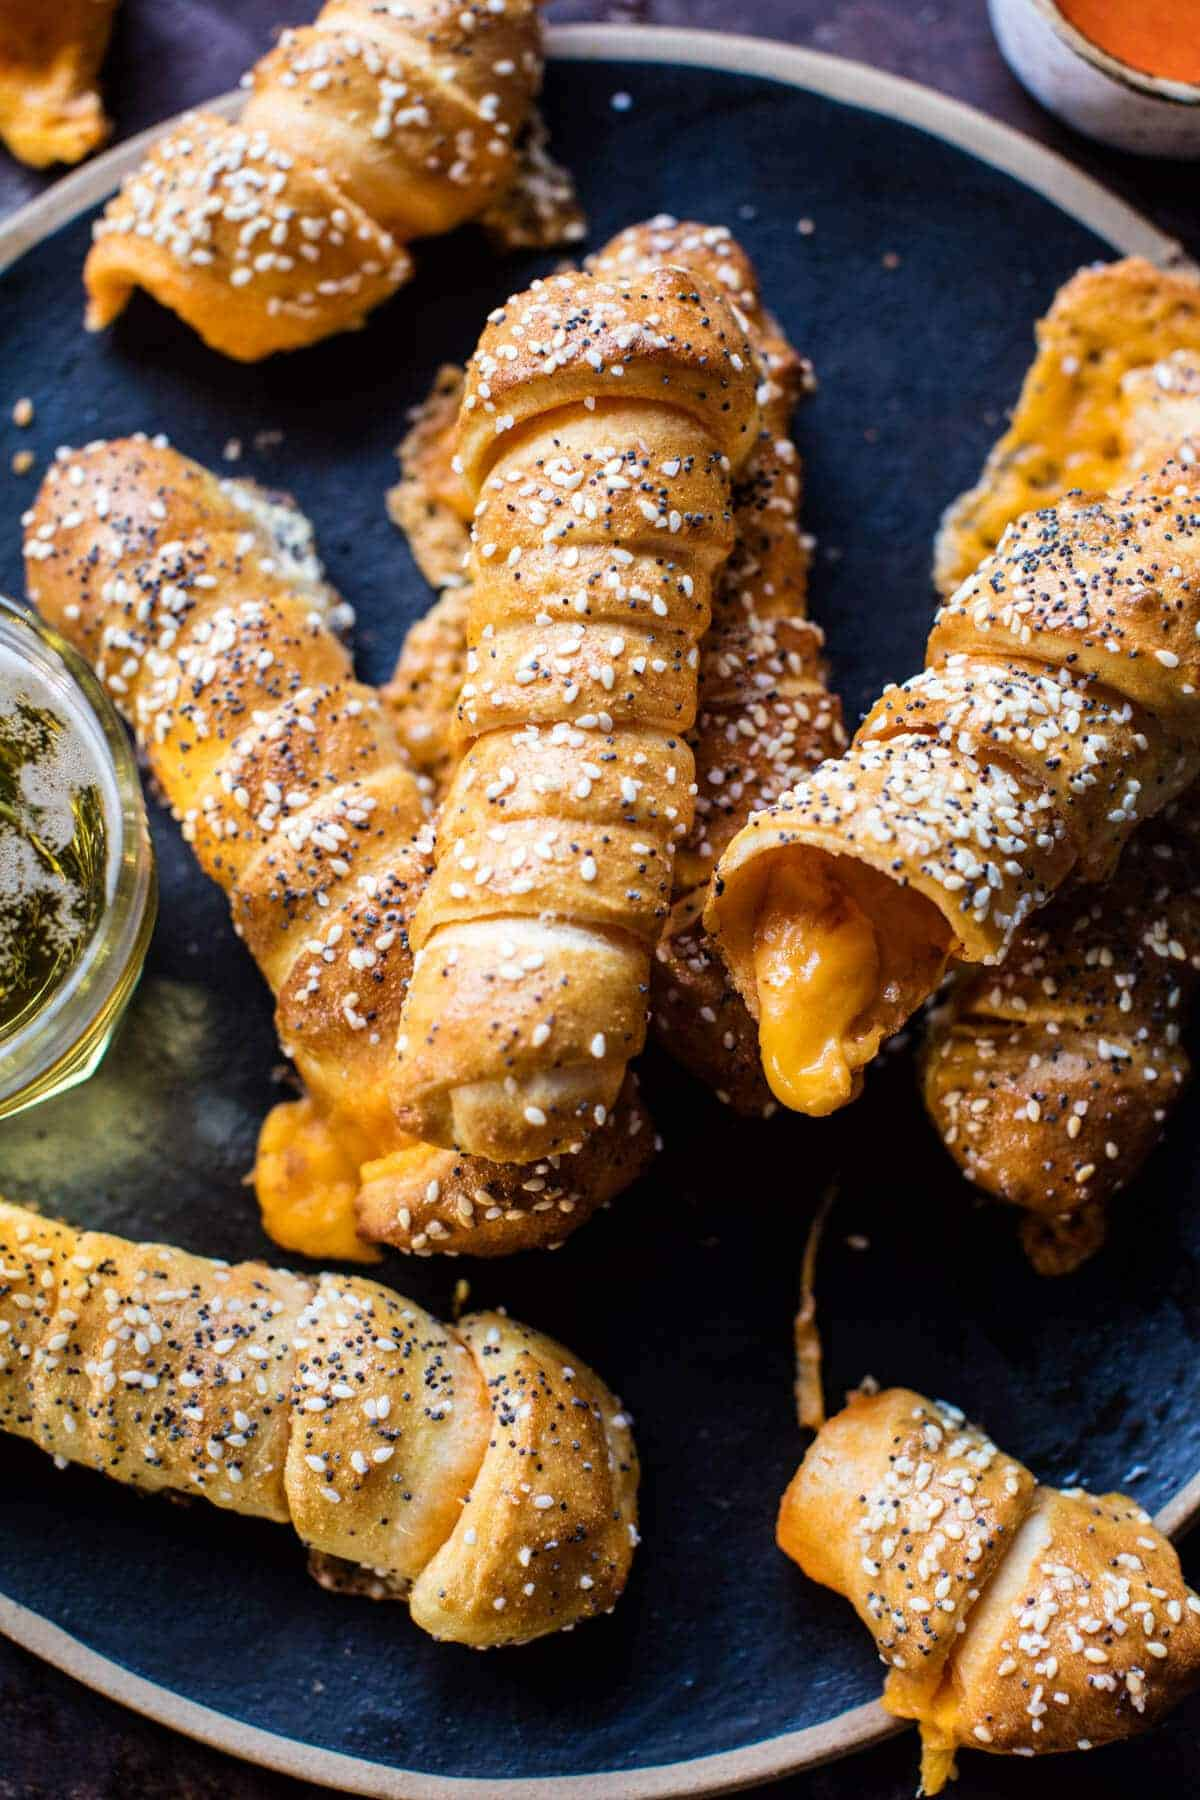
\includegraphics[width=1\textwidth,height=\textheight]{images/buffalo-cheddar-soft-pretzel-twists-with-everything-spice-.jpg}

\textbf{Prep Time:} 15 min \textbar{} \textbf{Cook Time:} 15 min
\textbar{} \textbf{Total Time:} 30 min

\section{Ingredients}\label{ingredients-144}

\begin{itemize}
\tightlist
\item
  1 1/2 cups warm water
\item
  2 tablespoons light brown sugar
\item
  2 1/4 teaspoons active dry yeast (( 1 packet))
\item
  1/2 cup (1 stick) unsalted butter (melted)
\item
  1 1/2 teaspoons kosher salt
\item
  4 1/2 cups all-purpose flour
\item
  1/2 cup buffalo sauce (plus more for serving)
\item
  16 cheddar cheese sticks
\item
  2/3 cup baking soda (for boiling the pretzels)
\item
  1 egg (beaten, for brushing before baking)
\item
  3 tablespoons toasted white sesame seeds
\item
  2 tablespoons poppy seeds
\item
  2 teaspoons dried onion
\item
  2 teaspoons dried garlic
\item
  2 teaspoons kosher or coarse salt
\end{itemize}

\section{Instructions}\label{instructions-144}

\begin{enumerate}
\def\labelenumi{\arabic{enumi}.}
\tightlist
\item
  Combine the water, brown sugar and yeast in the bowl of a stand mixer
  and mix with the dough hook until combined. Let sit for 5 minutes. Add
  the melted butter, 1 1/2 teaspoons kosher salt and the all-purpose
  flour to the mixture and mix on low speed until combined. Increase the
  speed to medium and continue kneading until the dough is smooth and
  begins to pull away from the sides of the bowl, about 3 to 4 minutes.
  If the dough appears too wet, add additional flour, 1 tablespoon at a
  time. Remove the dough from the bowl and coat the bowl with olive oil,
  add the dough and turn to coat. Cover with plastic wrap and place in a
  warm spot until the dough doubles in size, about 1 hour.
\item
  Preheat the oven to 425 degrees F. Bring a large pot of water to a
  boil and add the baking soda.
\item
  Remove the dough from the bowl and place on a flat surface. Divide the
  dough in half and roll into a rectangle about 1/4 inch thick. Spread
  the dough with a little buffalo sauce. Cut the dough widthwise into
  6-8 strips about 1/2 inch wide. Wrap the dough around the cheese
  sticks with the buffalo sauce side facing inward. Seal at both ends.
  Boil the pretzels in the baking soda water, 1-2 at a time for 30
  seconds. Remove with a large flat slotted spatula or a spider. Place 8
  pretzels on each baking sheet, brush the tops with the egg wash.
\item
  To make the everything spice. In a small bowl, combine the sesame
  seeds, poppy seeds, dried onion, dried garlic, and 2 teaspoons salt.
  Sprinkle the spice mix generously over each pretzel. Bake for 10 to 15
  minutes or until pretzels are golden brown. Serve warm with extra
  buffalo sauce for dipping
\end{enumerate}

\bookmarksetup{startatroot}

\chapter{Winter Bliss Balls.}\label{winter-bliss-balls.}

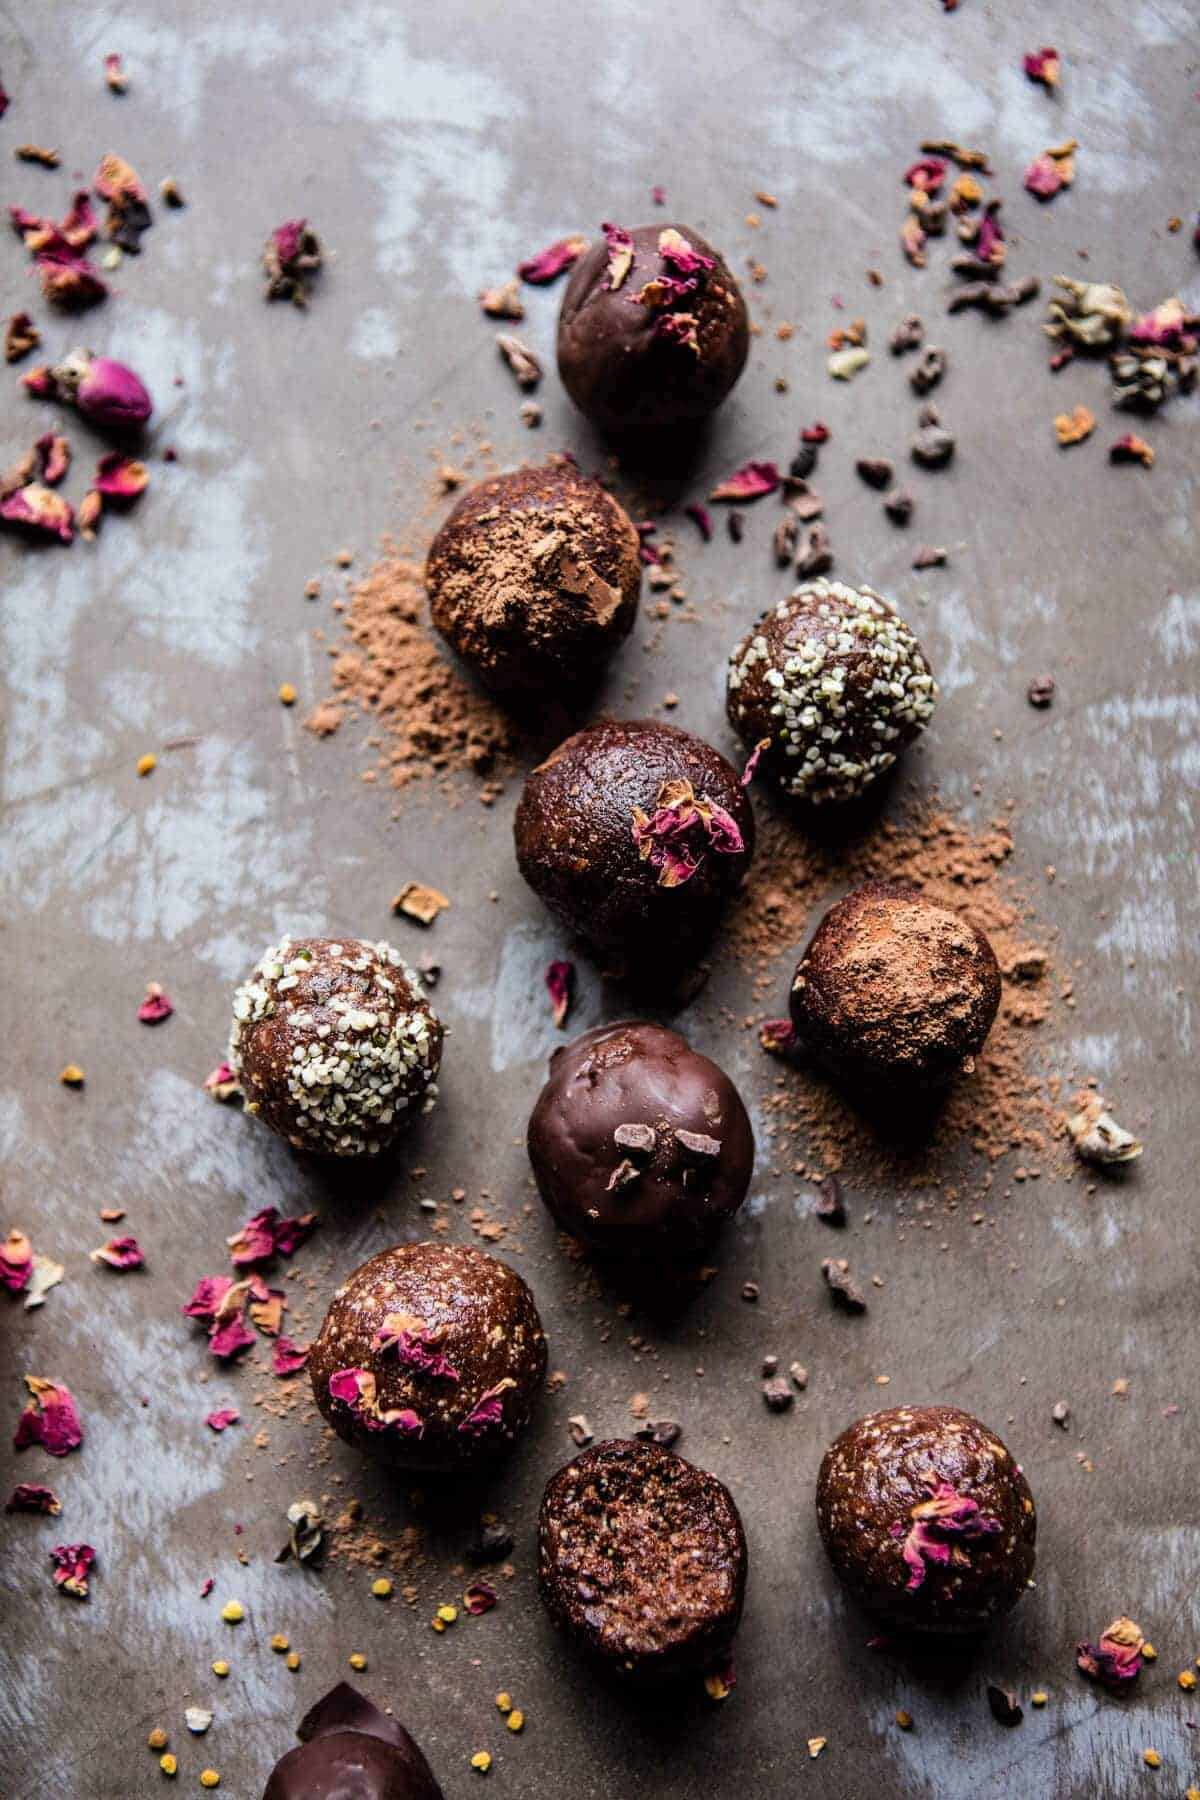
\includegraphics[width=1\textwidth,height=\textheight]{images/winter-bliss-balls-.jpg}

\textbf{Prep Time:} 10 min \textbar{} \textbf{Cook Time:} \textbar{}
\textbf{Total Time:} 10 min

\section{Ingredients}\label{ingredients-145}

\begin{itemize}
\tightlist
\item
  25-30 medjool dates, pitted (about 2 cups packed)
\item
  1 1/2 cups roasted cashews
\item
  1/2 cup unsweetened coconut flakes
\item
  1/4 cup cacao powder
\item
  1/4 cup hemp seeds
\item
  2 tablespoons chia seeds
\item
  2 teaspoon maca powder
\item
  1 tablespoon orange zest
\item
  pinch of flaky sea salt
\item
  melted chocolate, nuts,seeds, dried roses, cocoa or cacao powder, for
  topping
\end{itemize}

\section{Instructions}\label{instructions-145}

\begin{enumerate}
\def\labelenumi{\arabic{enumi}.}
\tightlist
\item
  Line a baking sheet with parchment paper.
\item
  Add all the ingredients to a food a processor and pulse until fully
  combined and the dough easily holds together when squeezed in your
  hand.
\item
  Roll the dough into tablespoon size balls. If desired, roll on your
  desired toppings OR dip in melted chocolate and sprinkle your toppings
  onto the chocolate. Allow the chocolate to set in the fridge.
\item
  Store the balls in an airtight container in the fridge for up to 1
  week.
\end{enumerate}

\bookmarksetup{startatroot}

\chapter{Orange Turmeric Crush.}\label{orange-turmeric-crush.}

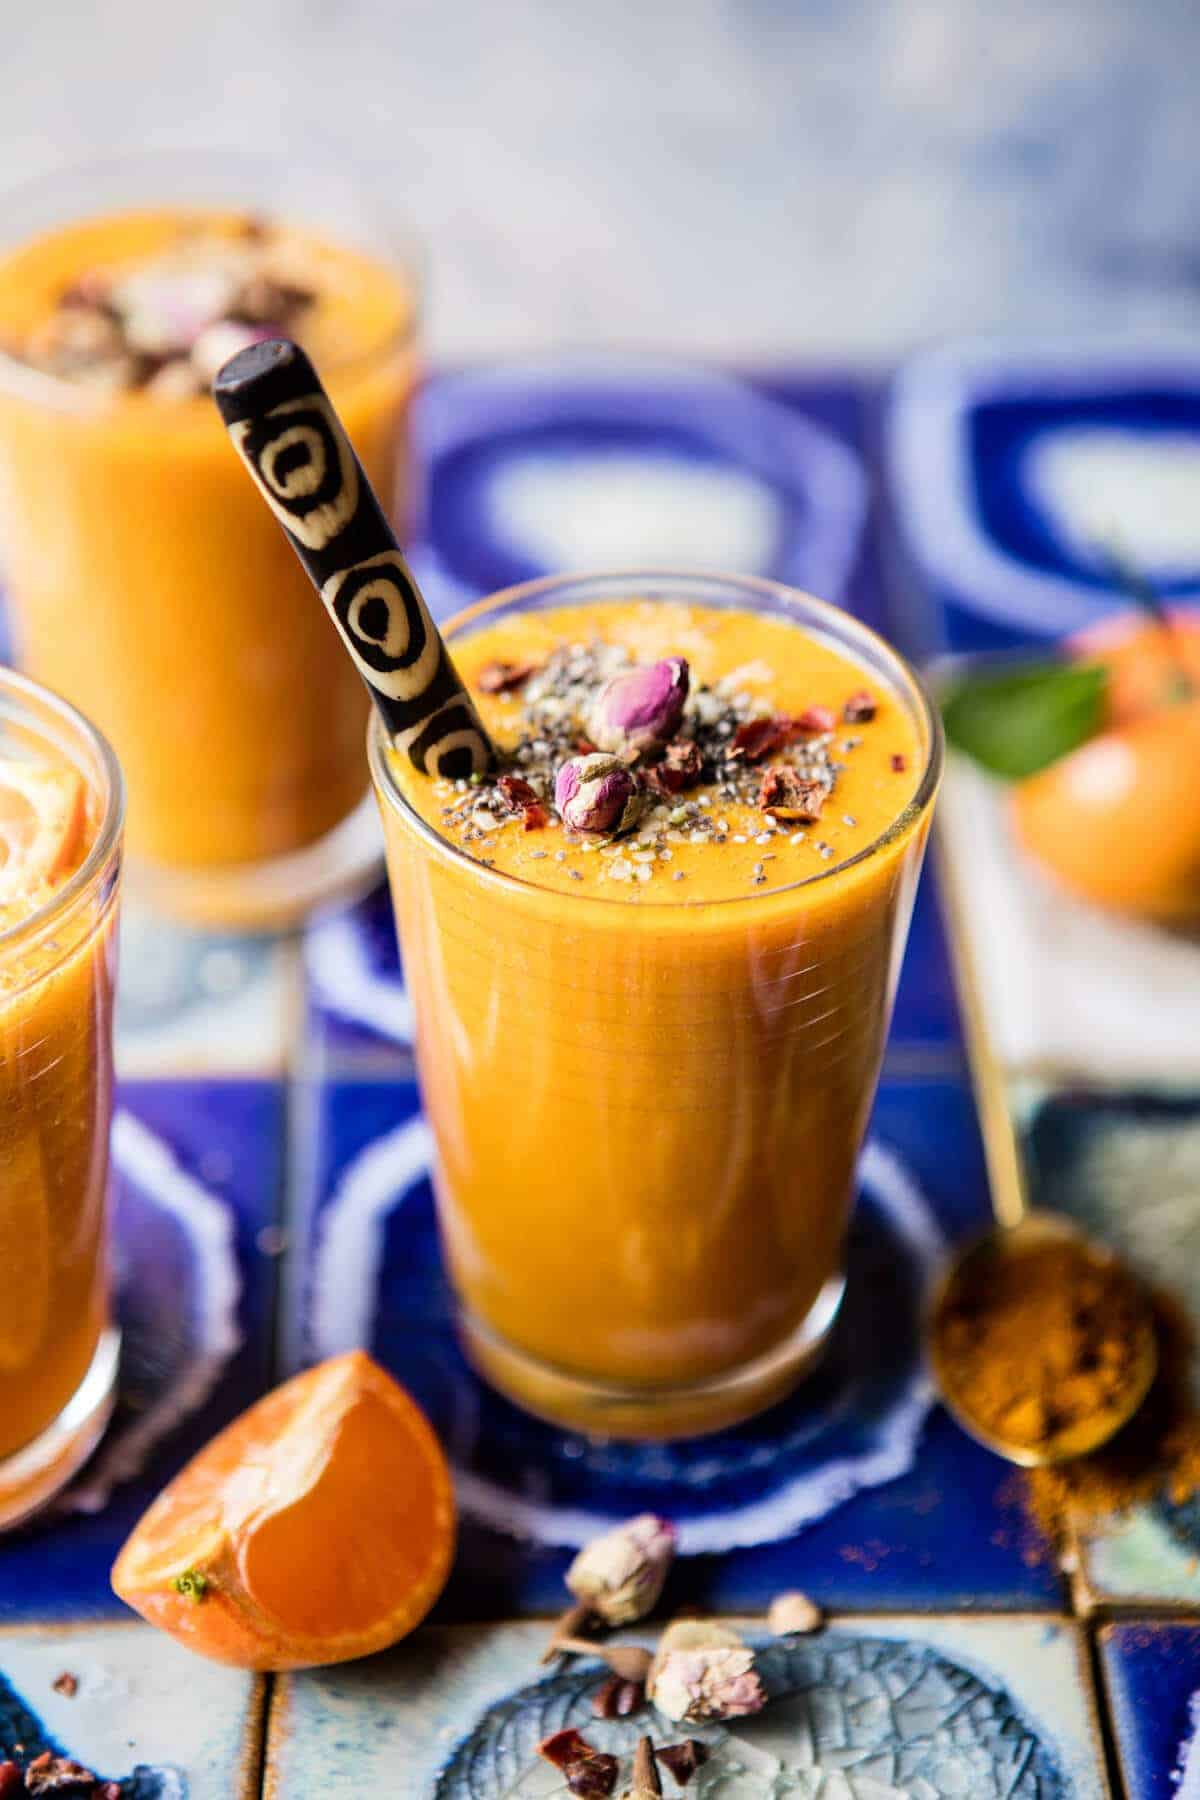
\includegraphics[width=1\textwidth,height=\textheight]{images/orange-turmeric-crush-.jpg}

\textbf{Prep Time:} 10 min \textbar{} \textbf{Cook Time:} \textbar{}
\textbf{Total Time:} 10 min

\section{Ingredients}\label{ingredients-146}

\begin{itemize}
\tightlist
\item
  1 cup Not-From-Concentrate Florida’s Natural® Brand Orange Juice
\item
  1 cup coconut water
\item
  4 pitted medjool dates
\item
  1 medium carrot
\item
  1/2 cup frozen mango chunks
\item
  1 teaspoon vanilla
\item
  1 teaspoon turmeric
\item
  1 teaspoon maca powder (optional)
\item
  pinch of salt
\item
  chia seeds (hemp seeds and or rose hips, for topping)
\end{itemize}

\section{Instructions}\label{instructions-146}

\begin{enumerate}
\def\labelenumi{\arabic{enumi}.}
\tightlist
\item
  In a high power blender, combine the orange juice, coconut water,
  dates, carrot, mango, vanilla, turmeric, maca power, and a pinch of
  salt. Add a large handful of ice and blend until completely smooth and
  creamy, about 3-5 minutes.
\item
  Divide between 2 glasses and top as desired. Enjoy!
\end{enumerate}

\bookmarksetup{startatroot}

\chapter{Chocolate Lovers Greek Yogurt Chocolate Mousse
Cake.}\label{chocolate-lovers-greek-yogurt-chocolate-mousse-cake.}

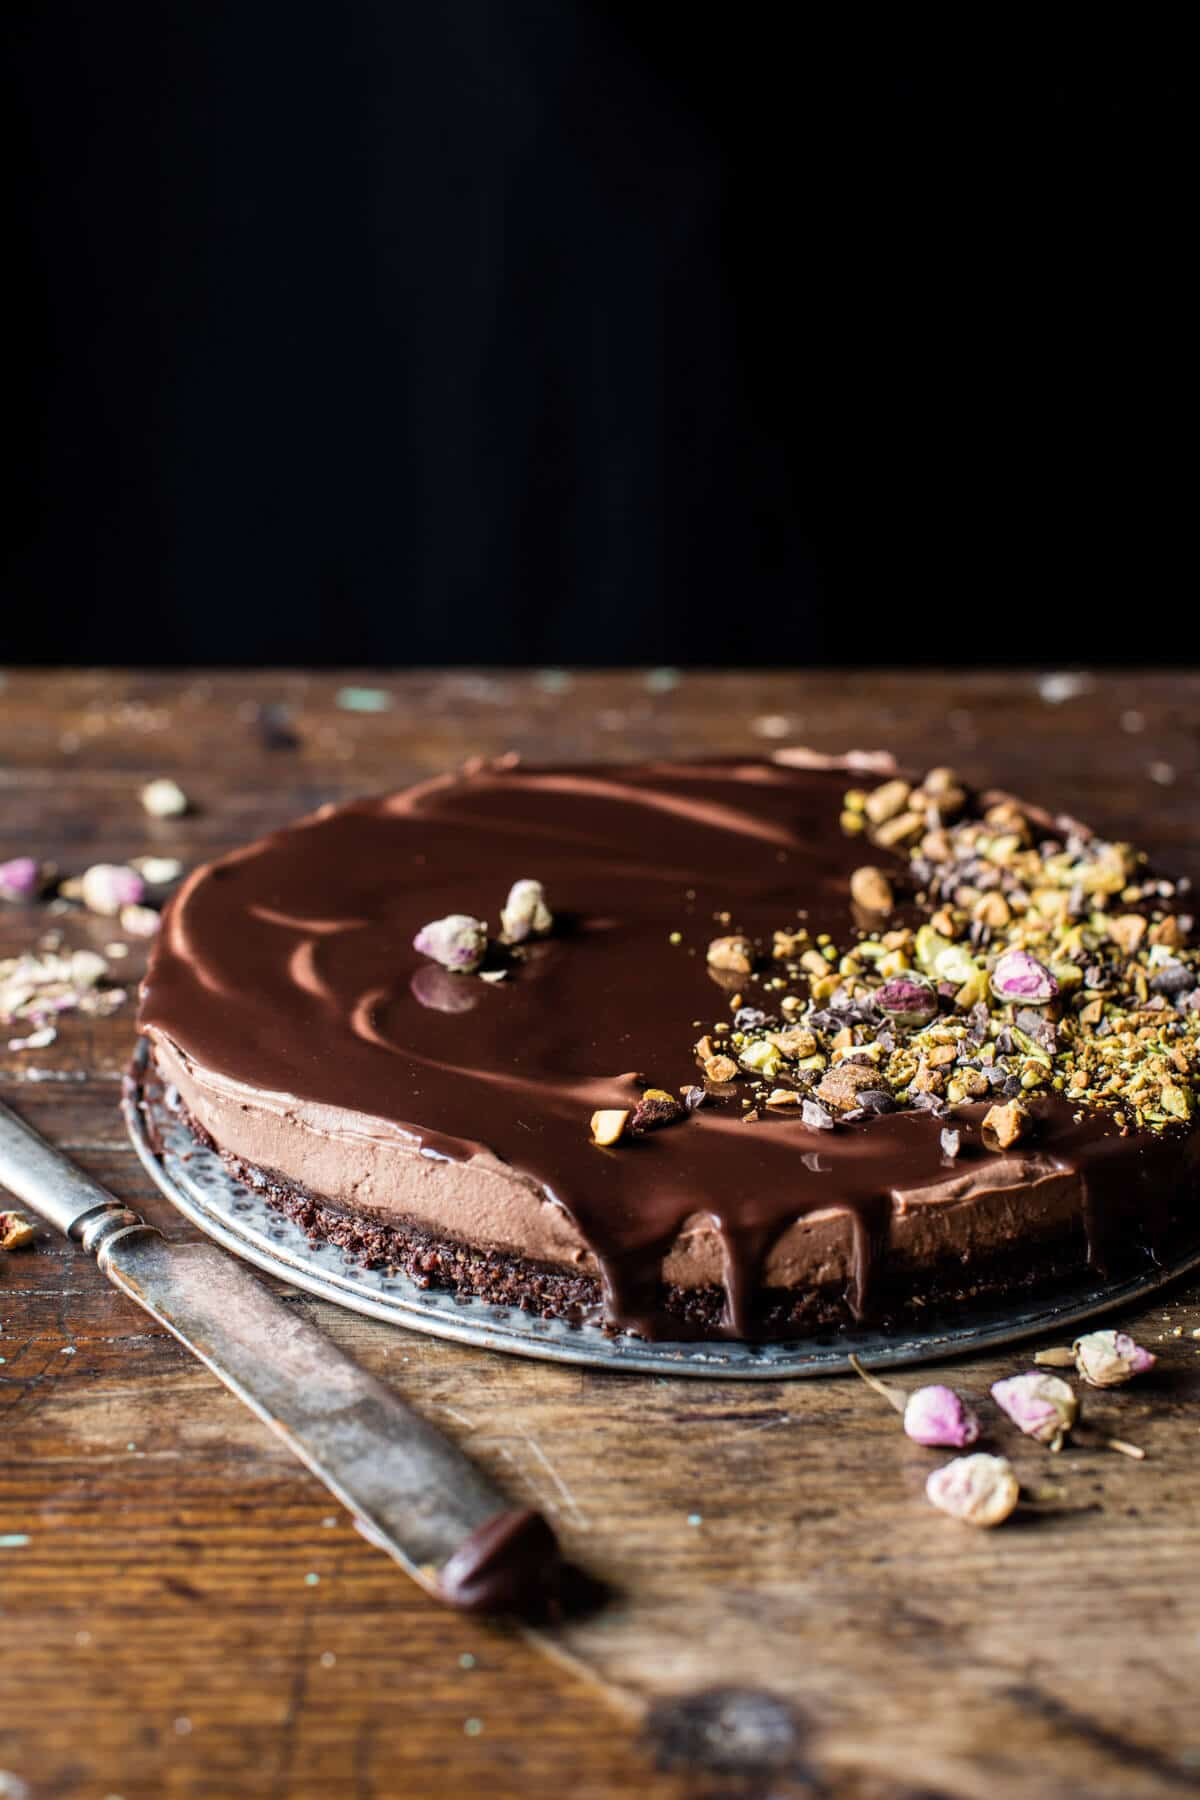
\includegraphics[width=1\textwidth,height=\textheight]{images/chocolate-lovers-greek-yogurt-chocolate-mousse-cake-.jpg}

\textbf{Prep Time:} 10 min \textbar{} \textbf{Cook Time:} 3 min
\textbar{} \textbf{Total Time:} 1 hr 43 min

\section{Ingredients}\label{ingredients-147}

\begin{itemize}
\tightlist
\item
  1 cup raw walnuts
\item
  1/2 cup raw (unsweetened coconut flakes)
\item
  1 1/2 cups pitted (packed dates (about 10 ounces))
\item
  1/2 cup cacao powder or unsweetened cocoa powder
\item
  pinch of flaky sea salt
\item
  1 cup heavy cream
\item
  1 1/2 cups plain whole milk greek yogurt
\item
  1/2 cup cacao powder or unsweetened cocoa powder
\item
  1-2 tablespoons honey
\item
  2 teaspoons vanilla
\item
  3/4 cup full-fat canned coconut milk or heavy cream
\item
  5 ounces dark chocolate (chopped)
\item
  chopped pistachios (for topping (optional)
\end{itemize}

\section{Instructions}\label{instructions-147}

\begin{enumerate}
\def\labelenumi{\arabic{enumi}.}
\tightlist
\item
  To make the crust. In a food processor, combine the walnuts, coconut,
  dates, cacao powder, and a pinch of salt. Pulse until finely ground
  and the mix forms a ball, about 5 minutes. Press the mixture into the
  bottom of an 8-9 inch spring form pan, making sure to pack it in
  tightly.
\item
  To make the mousse. Add the heavy cream to the bowl of a stand mixer
  fitted with the whisk attachment or use a hand held mixer. Whisk the
  cream until stiff peaks form. Using a spatula, gently fold the greek
  yogurt into the whipped cream. Add the cacao powder, honey, and
  vanilla and stir until combined and creamy. Spread the mousse evenly
  over top the brownie layer. Cover and place in the fridge for 1 1/2
  hours
\item
  In a microwave safe bowl, combine the coconut milk and dark chocolate.
  Microwave on power lever high for 30 second intervals, stirring after
  each until melted and smooth. Let cool five minutes, then pour the
  ganache over top the mouse. Sprinkle with pistachios. Chill 30 minutes
  or until ready serve.
\item
  Run a knife around the inside of the spring form pan and then release
  the cake from the pan. slice and serve!
\end{enumerate}

\bookmarksetup{startatroot}

\chapter{Healthier Tempeh Reuben.}\label{healthier-tempeh-reuben.}

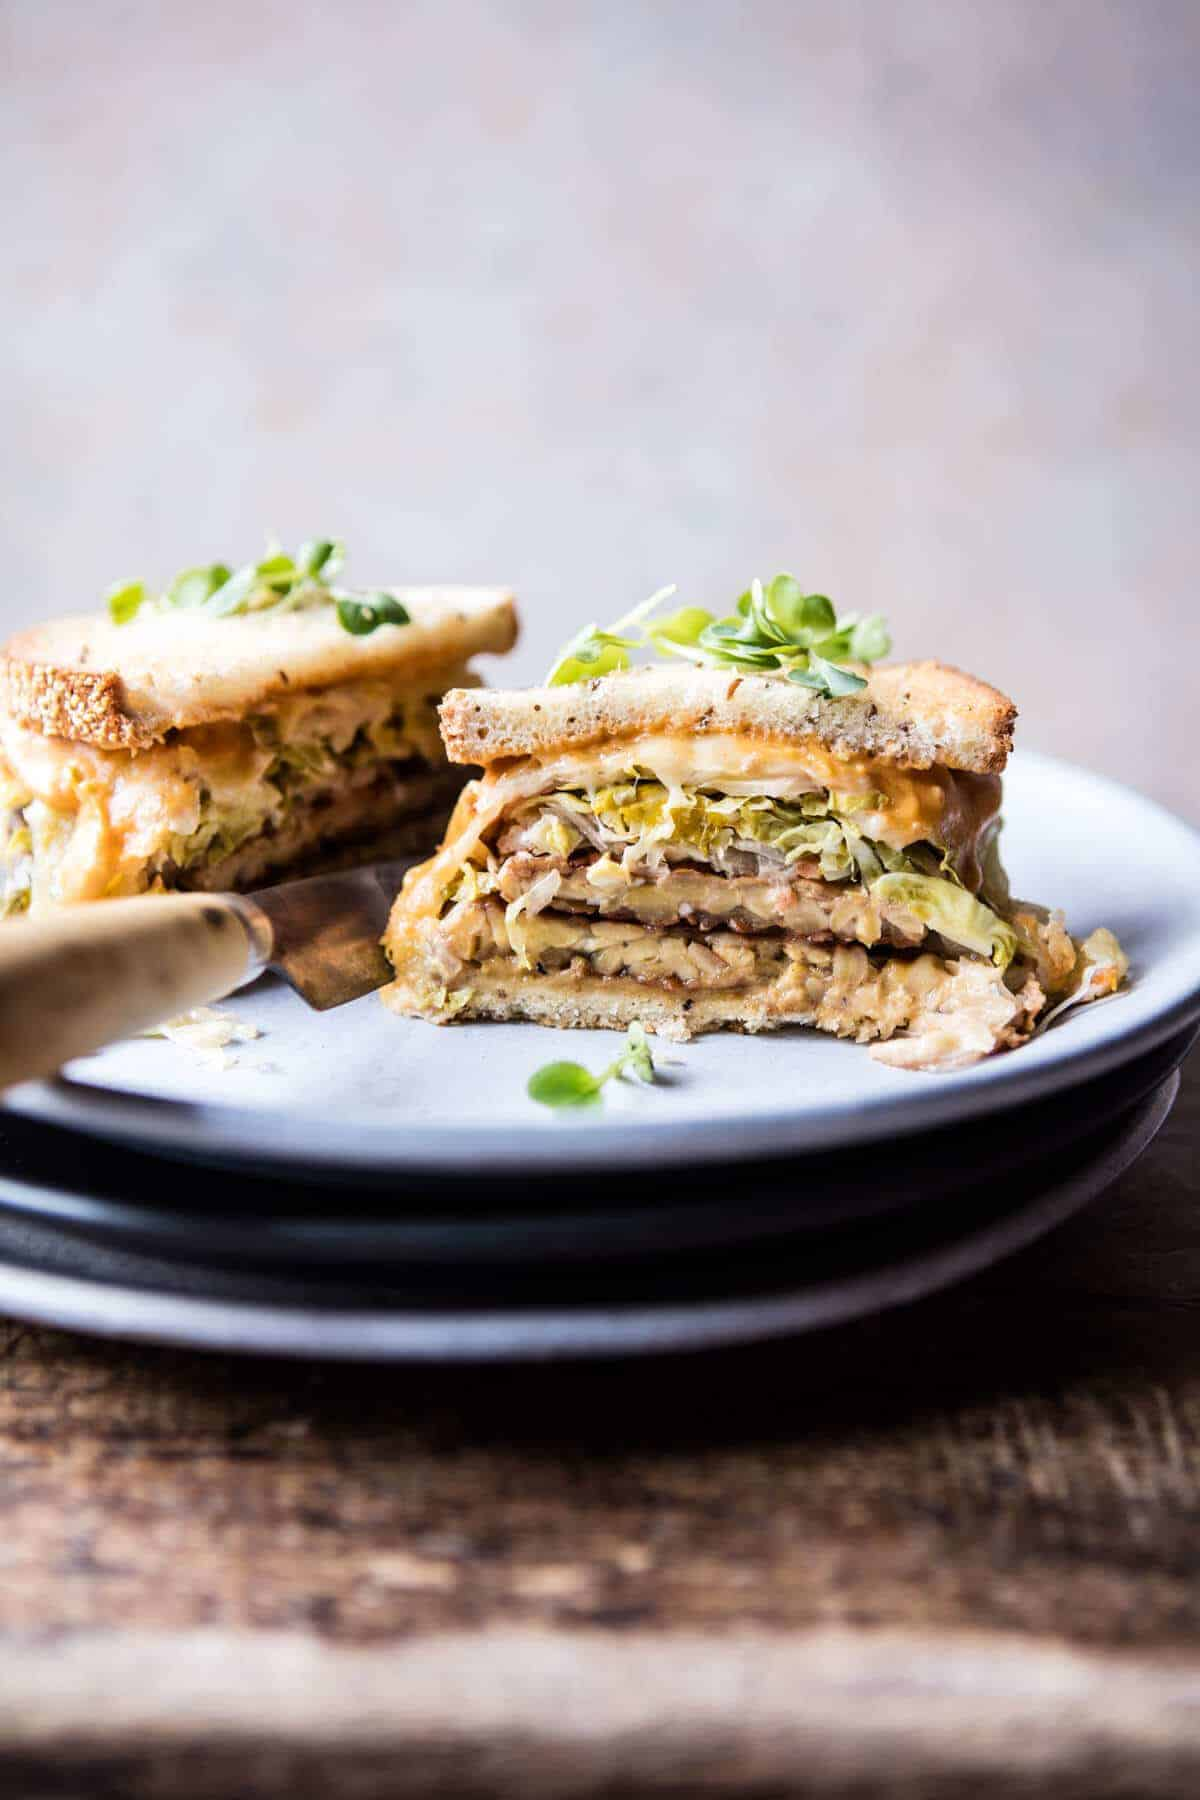
\includegraphics[width=1\textwidth,height=\textheight]{images/healthier-tempeh-reuben-.jpg}

\textbf{Prep Time:} 10 min \textbar{} \textbf{Cook Time:} 15 min
\textbar{} \textbf{Total Time:} 25 min

\section{Ingredients}\label{ingredients-148}

\begin{itemize}
\tightlist
\item
  8 ounces brown rice tempeh
\item
  1/4 cup low sodium soy sauce or tamari
\item
  black pepper
\item
  1 tablespoon mustard seeds
\item
  4 slices rye bread
\item
  2 tablespoons organic butter
\item
  1/4 cup cashew cheese (optional, recipe follows)
\item
  1 cup sauerkraut
\item
  2 slices swiss cheese
\item
  3/4 cup tahini
\item
  1-2 tablespoons chili sauce
\item
  juice of 1/2 a lemon
\item
  1 tablespoon chopped pickle + 1 tablespoon pickle juice
\item
  1 tablespoon chopped chives
\item
  kosher salt + pepper
\end{itemize}

\section{Instructions}\label{instructions-148}

\begin{enumerate}
\def\labelenumi{\arabic{enumi}.}
\tightlist
\item
  Slice the tempeh in half lengthwise and then slice each piece in half
  to create 4 small, thin pieces.
\item
  In a gallon size zip top bag, combine the tempeh, soy sauce, pinch of
  black pepper, and mustard seeds. Seal the bag and gently toss to
  evenly coat. Let marinate for 30 minutes, flipping the bag around half
  way through.
\item
  Preheat the oven to 425 degrees F.
\item
  Heat a large skillet over medium high heat and add the olive oil. When
  the oil shimmers, add the tempeh in batches and cook until golden
  crisp, about 3-5 minutes per side. Repeat with the remaining tempeh.
\item
  Spread the butter over each piece of bread and toast in the oven on a
  baking sheet for 3-5 minutes. Remove the bread. Spread the bottom
  pieces of bread with cashew cheese. Add the tempeh, sauerkraut, and
  swiss cheese. Return the baking sheet to the oven to melt the cheese,
  about 5 minutes.
\item
  Meanwhile, make the Healthier 1000 Island Dressing. In a small bowl,
  whisk together the tahini, chili sauce, lemon juice, chopped pickles
  and pickle juice. Add water, 1 tablespoon at a time, until the sauce
  is smooth and pourable. Stir in the chives and season with salt and
  pepper. Keep stored in the fridge for up to 2 weeks
\item
  Spread a little dressing on the inside of the remaining 2 pieces of
  bread. Remove the sandwiches from the oven and add the top piece of
  bread, dressing side facing down. Slice each sandwich in half. EAT.
\end{enumerate}

\bookmarksetup{startatroot}

\chapter{Superfood Cashew Goji Berry
Bars.}\label{superfood-cashew-goji-berry-bars.}

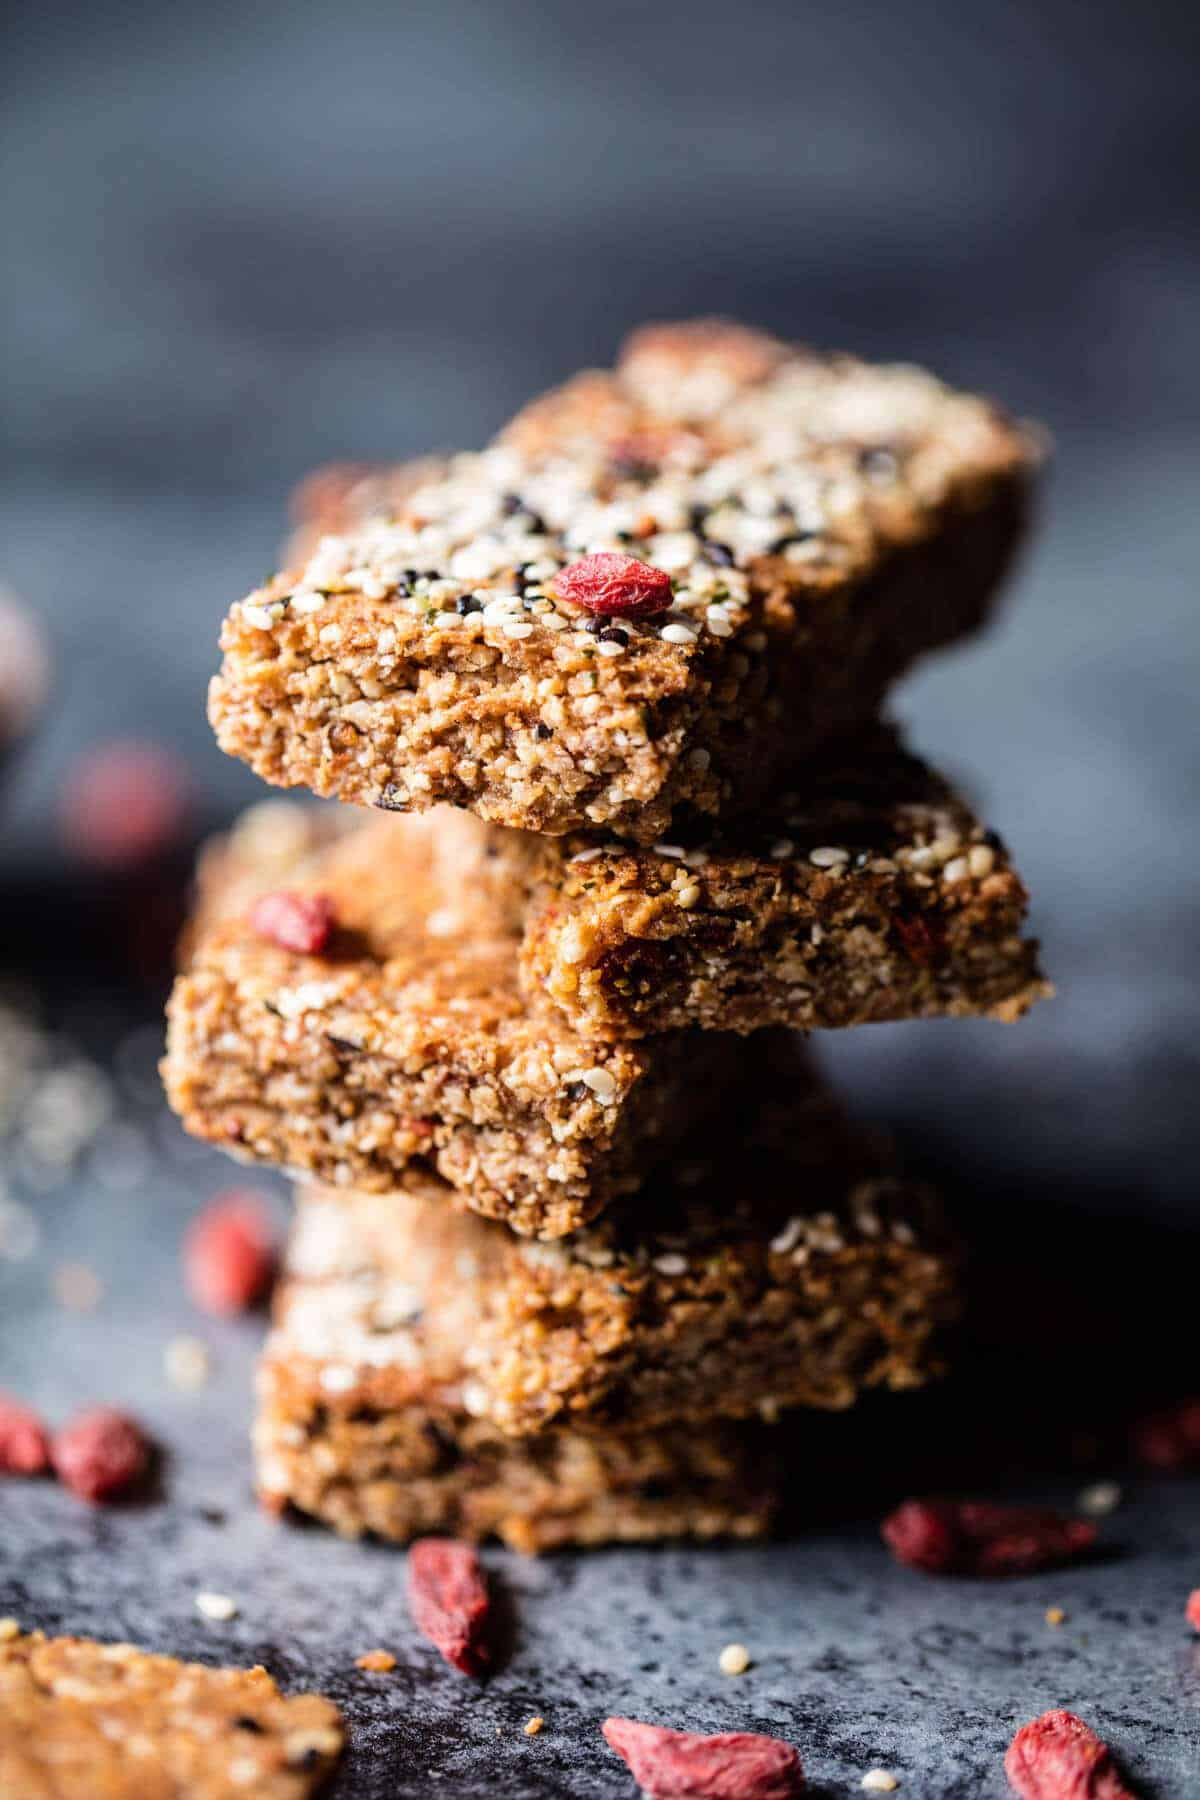
\includegraphics[width=1\textwidth,height=\textheight]{images/superfood-cashew-goji-berry-bars-.jpg}

\textbf{Prep Time:} 15 min \textbar{} \textbf{Cook Time:} 40 min
\textbar{} \textbf{Total Time:} 55 min

\section{Ingredients}\label{ingredients-149}

\begin{itemize}
\tightlist
\item
  1 1/2 cups raw cashews
\item
  1/2 cup raw almonds
\item
  1 cup raw (unsweetened coconut flakes)
\item
  1/4 cup + 1 tablespoon sesame seeds
\item
  4 tablespoons hemp seeds
\item
  1/4 cup cooked quinoa
\item
  1/4 cup tahini
\item
  1 teaspoon kosher salt
\item
  1/4 teaspoon cinnamon
\item
  1/2 cup organic honey
\item
  1 tablespoon coconut oil
\item
  1 teaspoon vanilla extract
\item
  1/2 cup dried goji berries
\end{itemize}

\section{Instructions}\label{instructions-149}

\begin{enumerate}
\def\labelenumi{\arabic{enumi}.}
\tightlist
\item
  Preheat oven to 350 degrees F. Coat an 8x8 inch baking pan with
  cooking spray and then line with parchment paper. Set aside.
\item
  Toast the cashews, almonds, coconut, 1/4 cup sesame seeds, and 3
  tablespoons hemp on a baking sheet, stirring occasionally, until
  golden brown, about 8â€``12 minutes. Let cool slightly.
\item
  Add the toasted nuts and seeds, plus the quinoa, tahini, cinnamon, and
  salt to a food processor or high powdered blender. Process until
  finely chopped.
\item
  Bring the honey and the coconut oil to a boil in a small saucepan.
  Cook, stirring, for about 1 minute. Remove and stir in the vanilla.
  Pour over the cashew/seed mixture and stir to coat. Stir in the goji
  berries.
\item
  Press the mixture firmly into the prepared 8x8 pan with the back of a
  greased measuring cup or wet hands. Top the bars with the remaining 1
  tablespoon sesame and hemp seeds. Press the seeds gently to adhere.
\item
  Transfer to the oven and bake until golden brown, 25â€``30 minutes. Let
  cool, then cut into the bars. Store in an airtight container at room
  temp or in the fridge.
\end{enumerate}

\bookmarksetup{startatroot}

\chapter{Healthy Chai Banana
Pancakes.}\label{healthy-chai-banana-pancakes.}

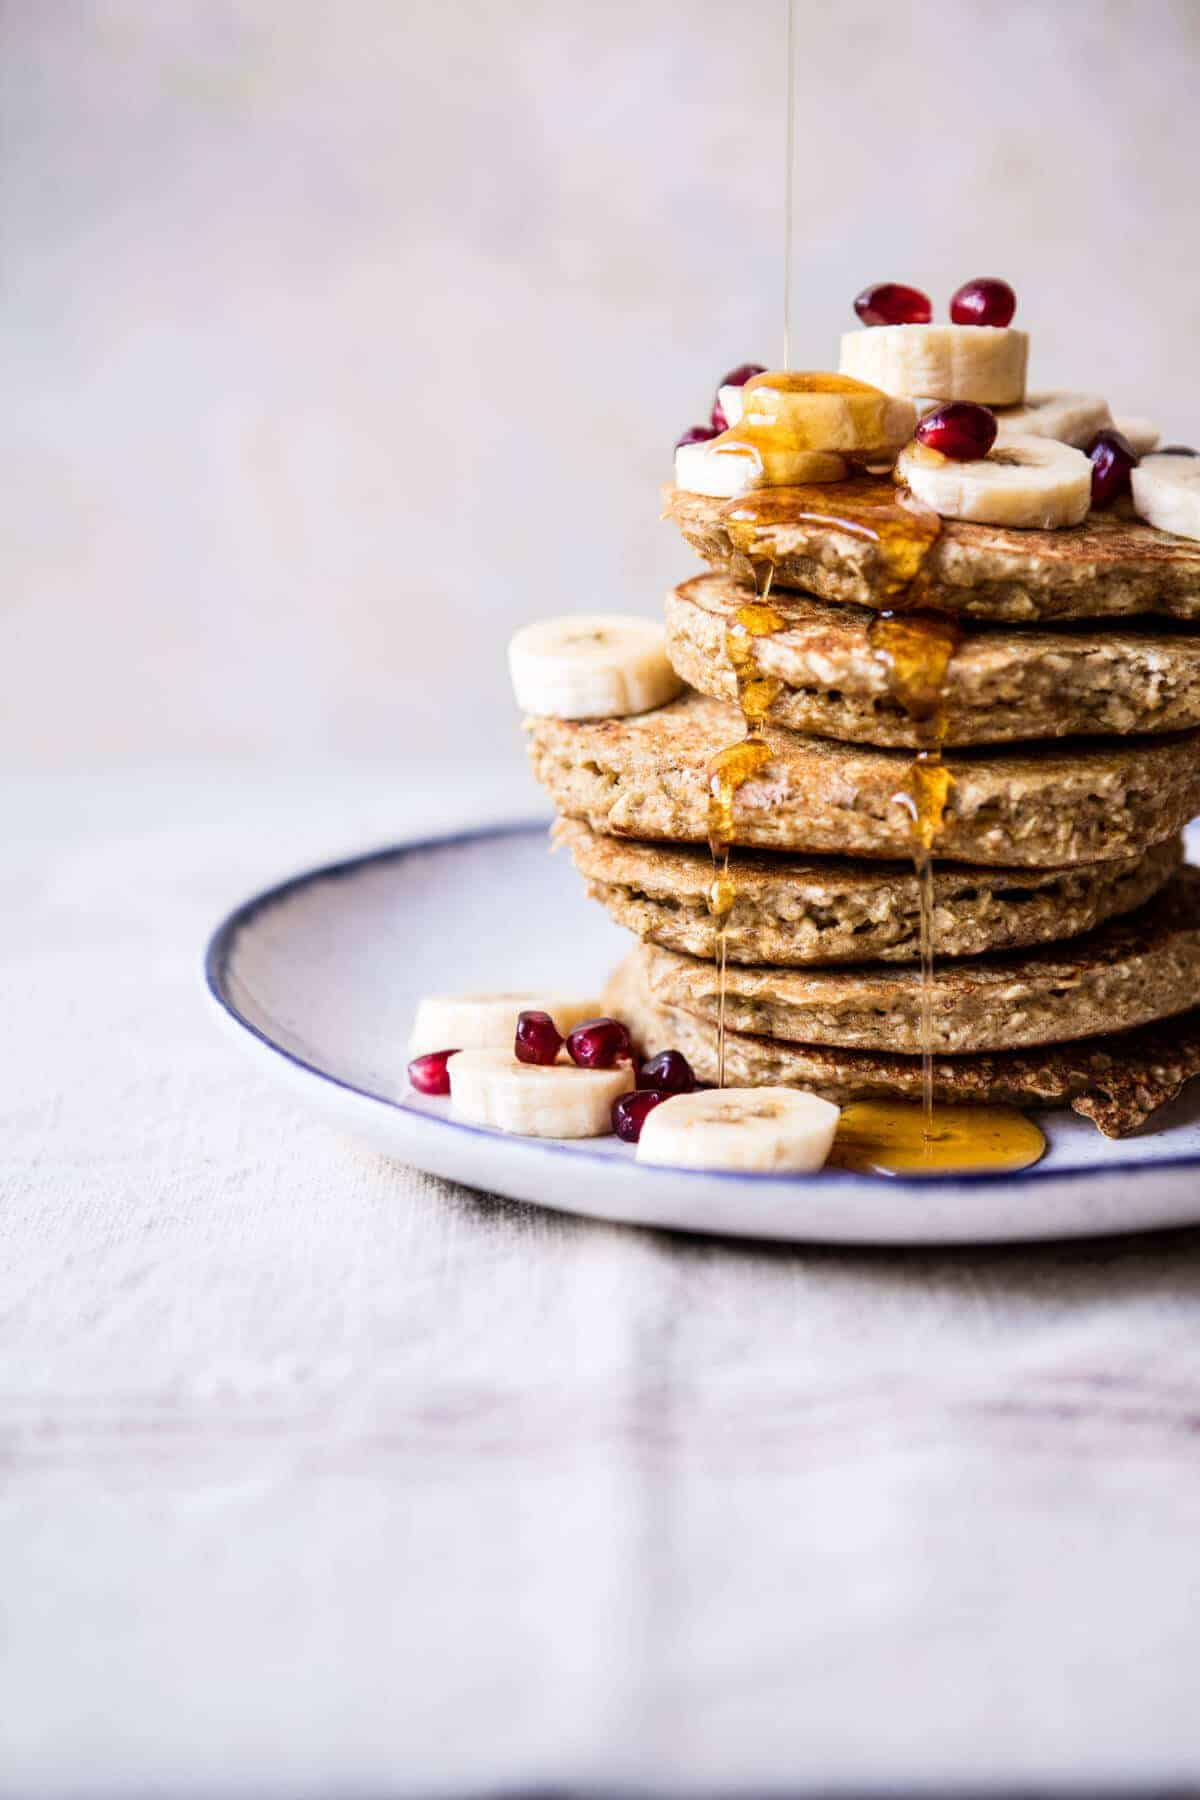
\includegraphics[width=1\textwidth,height=\textheight]{images/healthy-chai-banana-pancakes-.jpg}

\textbf{Prep Time:} 10 min \textbar{} \textbf{Cook Time:} 10 min
\textbar{} \textbf{Total Time:} 20 min

\section{Ingredients}\label{ingredients-150}

\begin{itemize}
\tightlist
\item
  2 whole eggs + 2 egg whites
\item
  1 medium/large ripe banana
\item
  1 cup old fashioned oats
\item
  2 teaspoons vanilla extract
\item
  1 teaspoon baking powder
\item
  1/2 teaspoon cinnamon
\item
  1/2 teaspoon ginger
\item
  1/4 teaspoon cardamon
\item
  1/4 teaspoon all-spice
\item
  1/4 teaspoon salt
\item
  maple syrup (bananas, and fresh fruit, for serving)
\end{itemize}

\section{Instructions}\label{instructions-150}

\begin{enumerate}
\def\labelenumi{\arabic{enumi}.}
\tightlist
\item
  In a blender, combine the eggs, egg whites, banana, oats, vanilla,
  baking powder, cinnamon, ginger, cardamon, all-spice, and salt. Blend
  until the oatmeal is finely ground and the mixture looks like pancake
  batter, about 30 seconds to 1 minute. It's OK if there are small
  chunks.
\item
  Heat a large skillet or griddle over medium heat and lightly grease
  the skillet with oil. Pour about 1/4 cup batter onto the center of the
  hot pan and gently spread the batter to form a circle. Cook until
  bubbles appear on the surface. Using a spatula, gently flip the
  pancake over and cook the other side for a minute, or until golden.
  Repeat with the remaining batter. Serve the pancakes with bananas,
  fresh fruit, and maple. Eat!
\end{enumerate}

\bookmarksetup{startatroot}

\chapter{Spicy Brown Rice Seared Tuna Roll Bowl with Mango
Chimichurri.}\label{spicy-brown-rice-seared-tuna-roll-bowl-with-mango-chimichurri.}

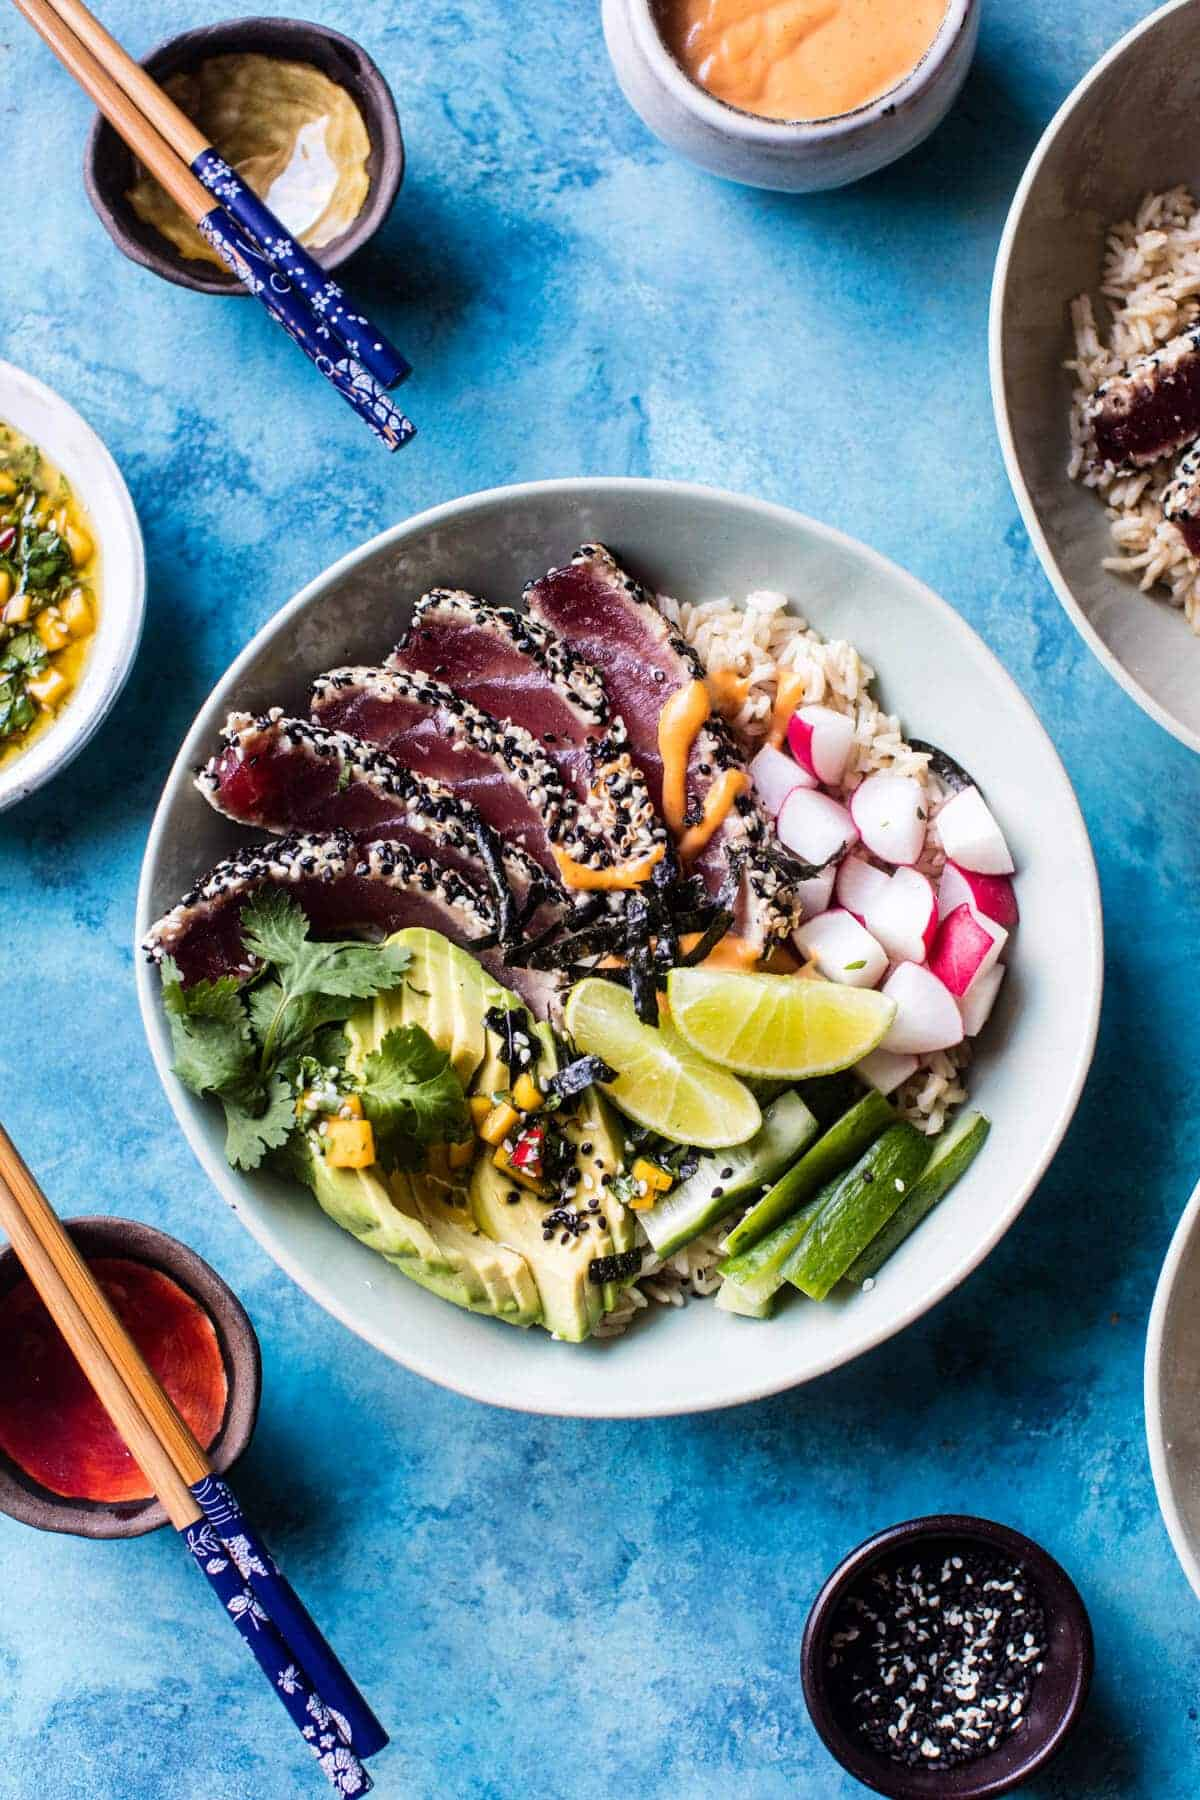
\includegraphics[width=1\textwidth,height=\textheight]{images/spicy-brown-rice-seared-tuna-roll-bowl-with-mango-chimichurri-.jpg}

\textbf{Prep Time:} 25 min \textbar{} \textbf{Cook Time:} 5 min
\textbar{} \textbf{Total Time:} 30 min

\section{Ingredients}\label{ingredients-151}

\begin{itemize}
\tightlist
\item
  1 mango (diced)
\item
  1/2 cup fresh cilantro (chopped)
\item
  1 Fresno chile pepper (seeded + chopped)
\item
  1 clove garlic (minced or grated)
\item
  1/4 cup low sodium soy sauce (plus more for serving)
\item
  1/4 cup rice vinegar
\item
  1/4 cup toasted sesame oil
\item
  juice of 1 lime
\item
  1/2 cup tahini
\item
  2 tablespoons sriracha
\item
  1 pound sushi grade tuna
\item
  1/4 cup black or white sesame seeds
\item
  2 teaspoons sesame oil
\item
  2-3 cups cooked brown rice
\item
  1 cucumber (cut into matchsticks)
\item
  4 radishes or daikon (sliced)
\item
  1 avocado (sliced)
\item
  4 thinly sliced or crumbled nori sheets
\end{itemize}

\section{Instructions}\label{instructions-151}

\begin{enumerate}
\def\labelenumi{\arabic{enumi}.}
\tightlist
\item
\end{enumerate}

\bookmarksetup{startatroot}

\chapter{Herbed Goat Cheese Stuffed
Mushrooms.}\label{herbed-goat-cheese-stuffed-mushrooms.}

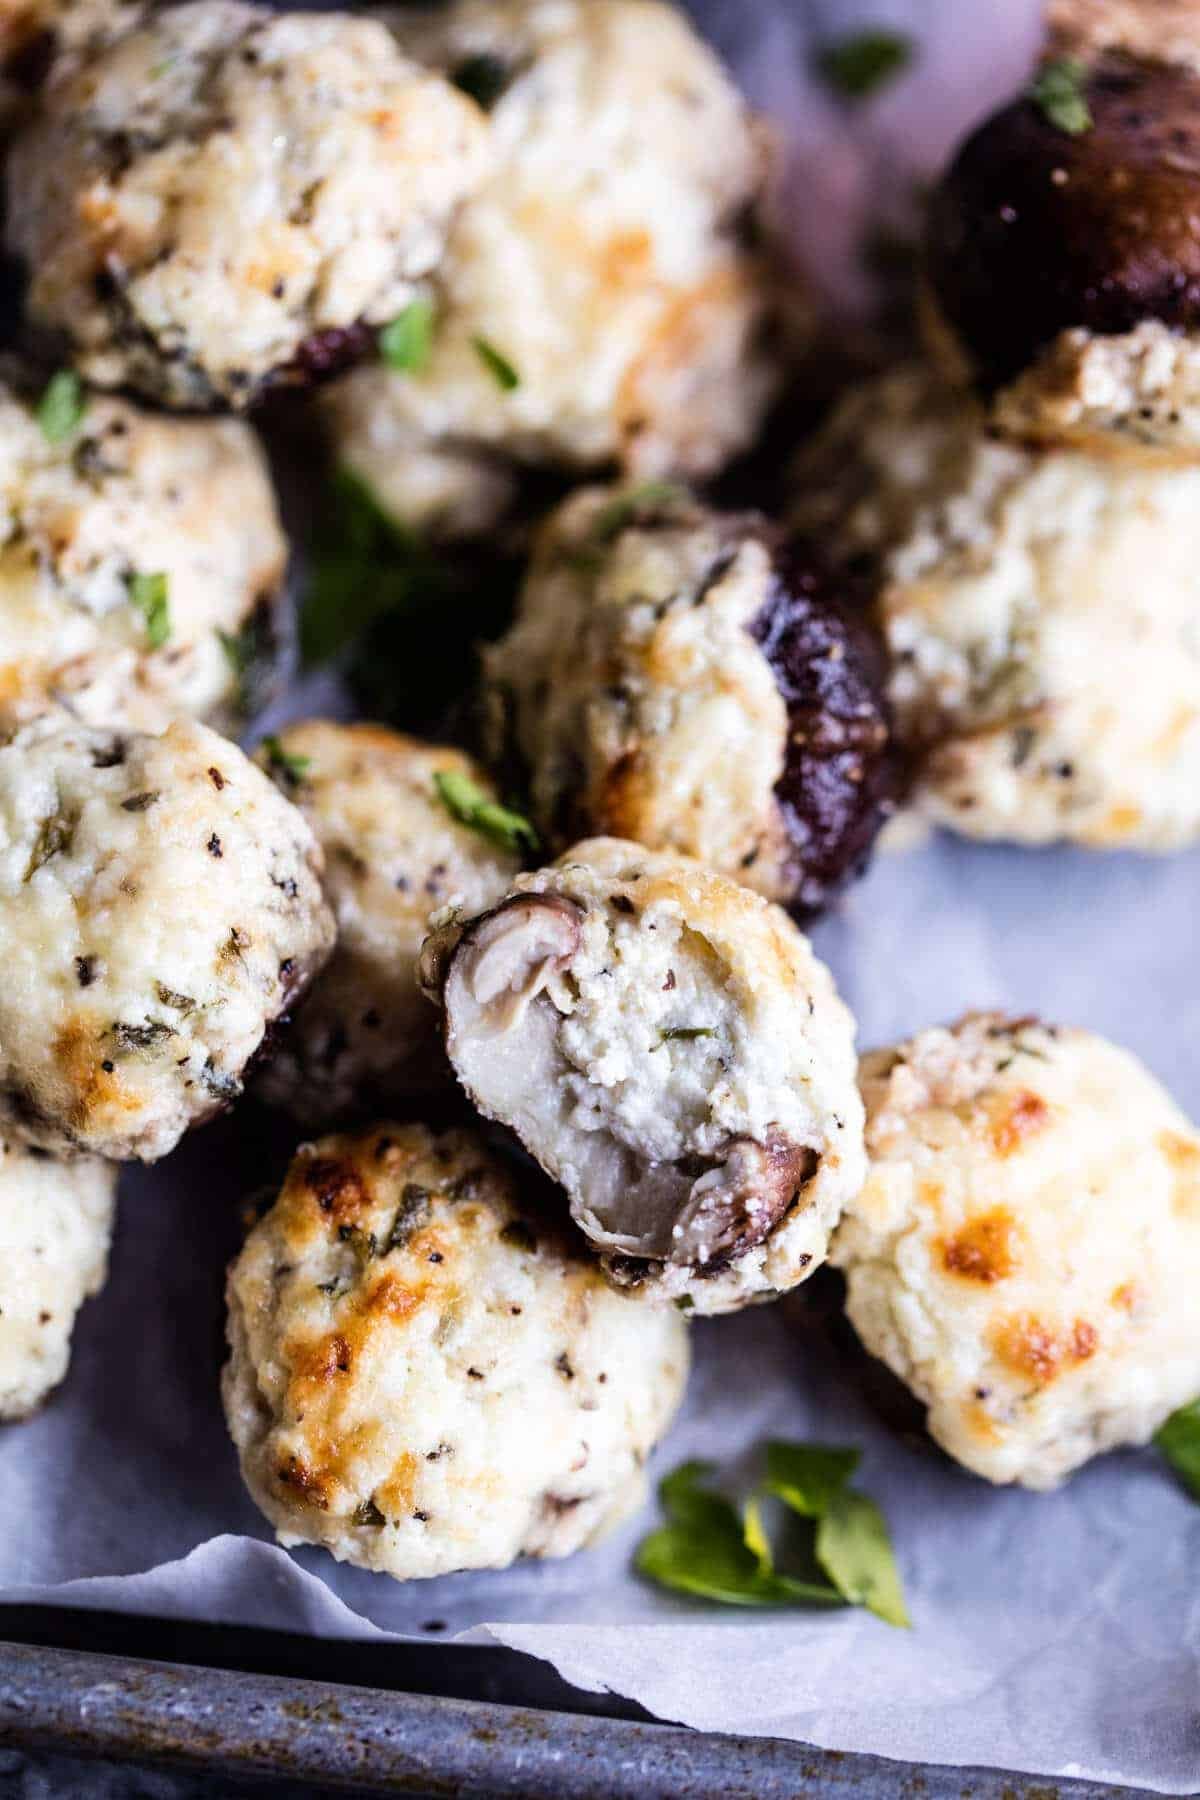
\includegraphics[width=1\textwidth,height=\textheight]{images/herbed-goat-cheese-stuffed-mushrooms-.jpg}

\textbf{Prep Time:} 10 min \textbar{} \textbf{Cook Time:} 20 min
\textbar{} \textbf{Total Time:} 30 min

\section{Ingredients}\label{ingredients-152}

\begin{itemize}
\tightlist
\item
  1 (8 ounce) log goat cheese
\item
  1 cup shredded fontina cheese
\item
  1/2 cup grated parmesan cheese
\item
  1 tablespoon chopped fresh thyme
\item
  1 tablespoon chopped fresh sage
\item
  1 tablespoon chopped chives
\item
  kosher salt and pepper
\item
  16 ounces cremini mushrooms (stems removed)
\end{itemize}

\section{Instructions}\label{instructions-152}

\begin{enumerate}
\def\labelenumi{\arabic{enumi}.}
\tightlist
\item
  Preheat the oven to 375 degrees F.
\item
  In a medium bowl, mix together the goat cheese, 1/2 cup fontina
  cheese, parmesan cheese, thyme, sage, chives, and a good pinch of both
  salt and pepper.
\item
  Remove the stems from the mushrooms and spoon the mixture into each
  mushroom cap, place on a baking sheet. Top with the remaining 1/2 cup
  fontina cheese. Transfer to the oven and bake for 20 to 25 minutes or
  until hot and bubbly. Serve warm!
\end{enumerate}

\bookmarksetup{startatroot}

\chapter{Santa's Nightcap.}\label{santas-nightcap.}

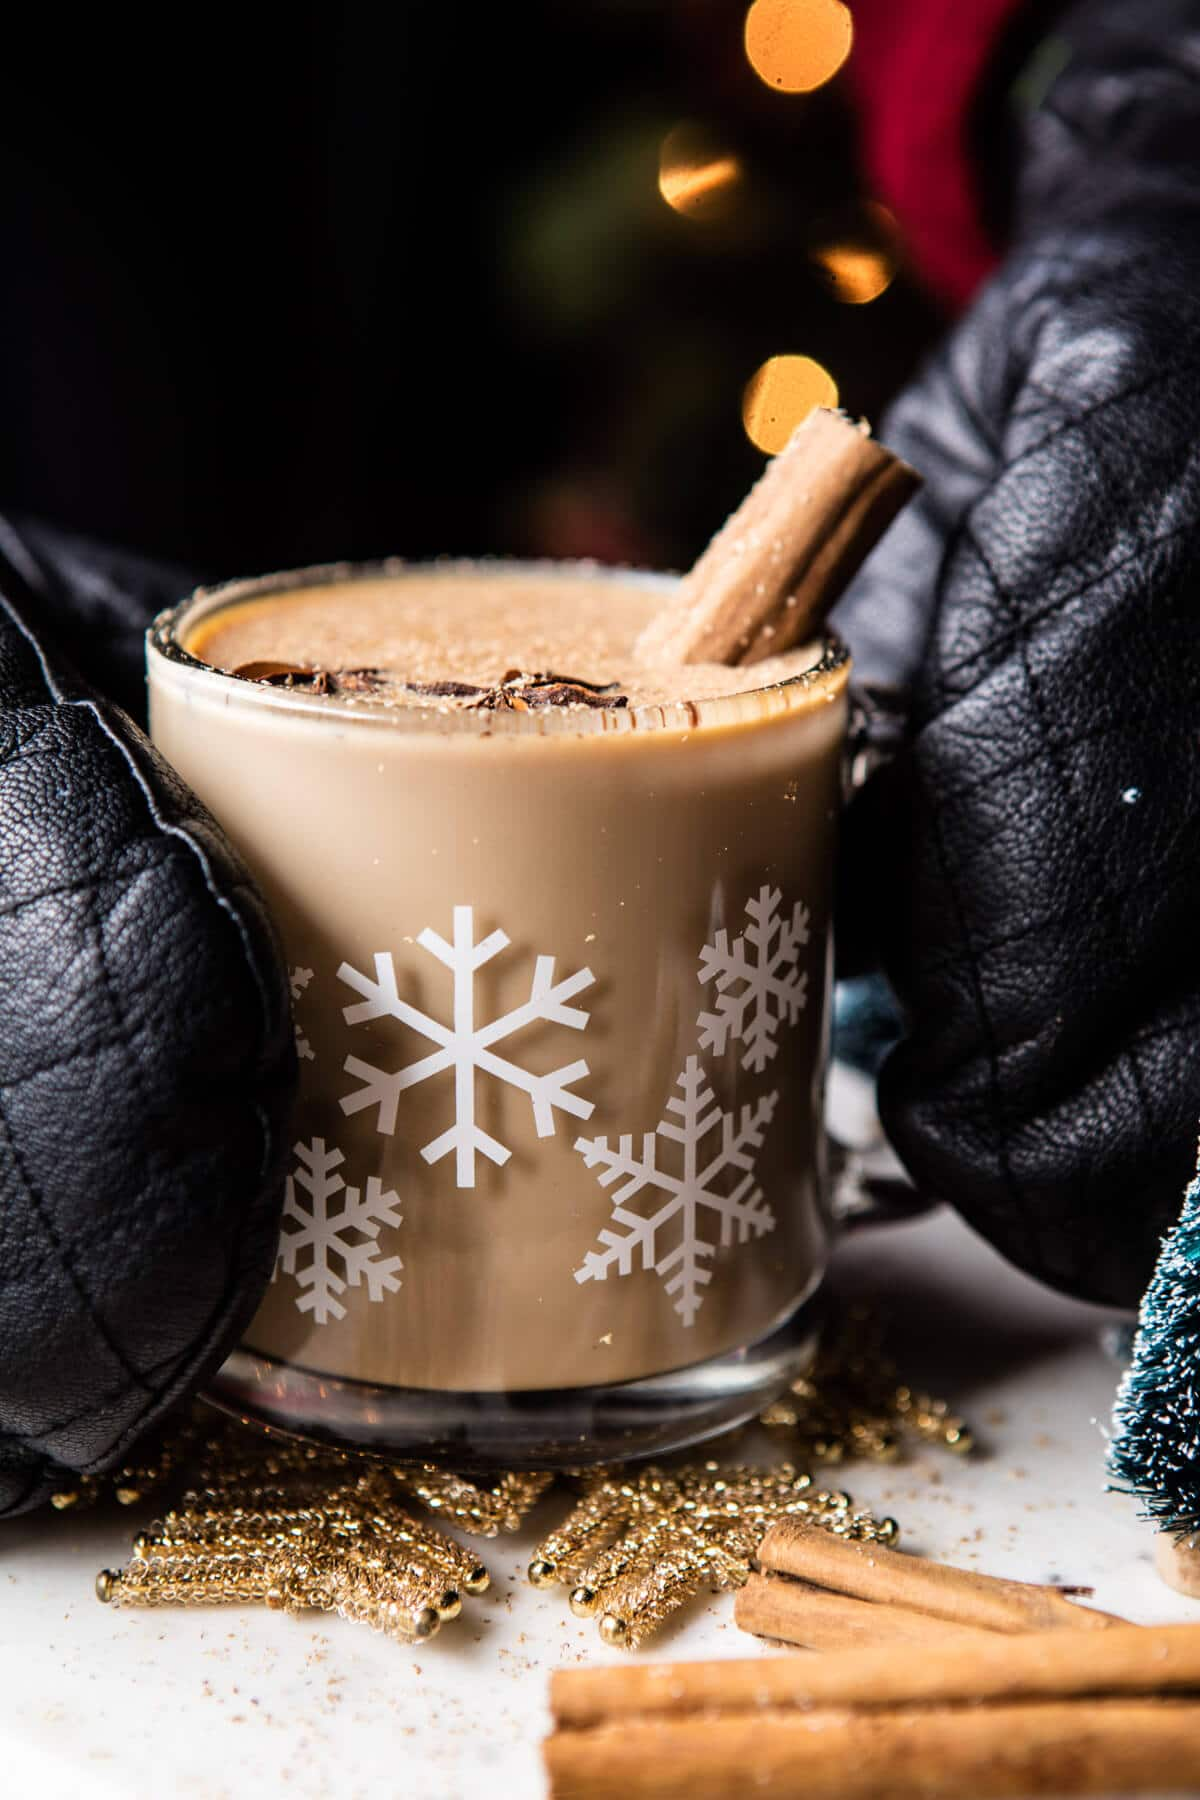
\includegraphics[width=1\textwidth,height=\textheight]{images/santa-s-nightcap-.jpg}

\textbf{Prep Time:} 10 min \textbar{} \textbf{Cook Time:} 20 min
\textbar{} \textbf{Total Time:} 30 min

\section{Ingredients}\label{ingredients-153}

\begin{itemize}
\tightlist
\item
  8 chai tea bags
\item
  4 cups whole milk
\item
  1/3 cup honey
\item
  2 cinnamon sticks
\item
  2 inch piece of fresh ginger
\item
  1 1/2 cups bourbon
\end{itemize}

\section{Instructions}\label{instructions-153}

\begin{enumerate}
\def\labelenumi{\arabic{enumi}.}
\tightlist
\item
  Bring 6 cups of water to a boil in a large pot. Remove from the heat,
  add the tea bags, cover and let steep for 15-30 minutes. Remove the
  tea bags and stir in the milk, and honey. Place the pot over medium
  heat. Add the cinnamon sticks and ginger, cook stirring often until
  the mixture is steaming. Stir in the bourbon.
\item
  Ladle the drink into mugs. Dust with cinnamon if desired. Drink up!
\item
  Alternately, you can chill the cocktail and serve cold over ice.
\end{enumerate}

\bookmarksetup{startatroot}

\chapter{Salted Caramel Chocolate Covered
Pretzels.}\label{salted-caramel-chocolate-covered-pretzels.}

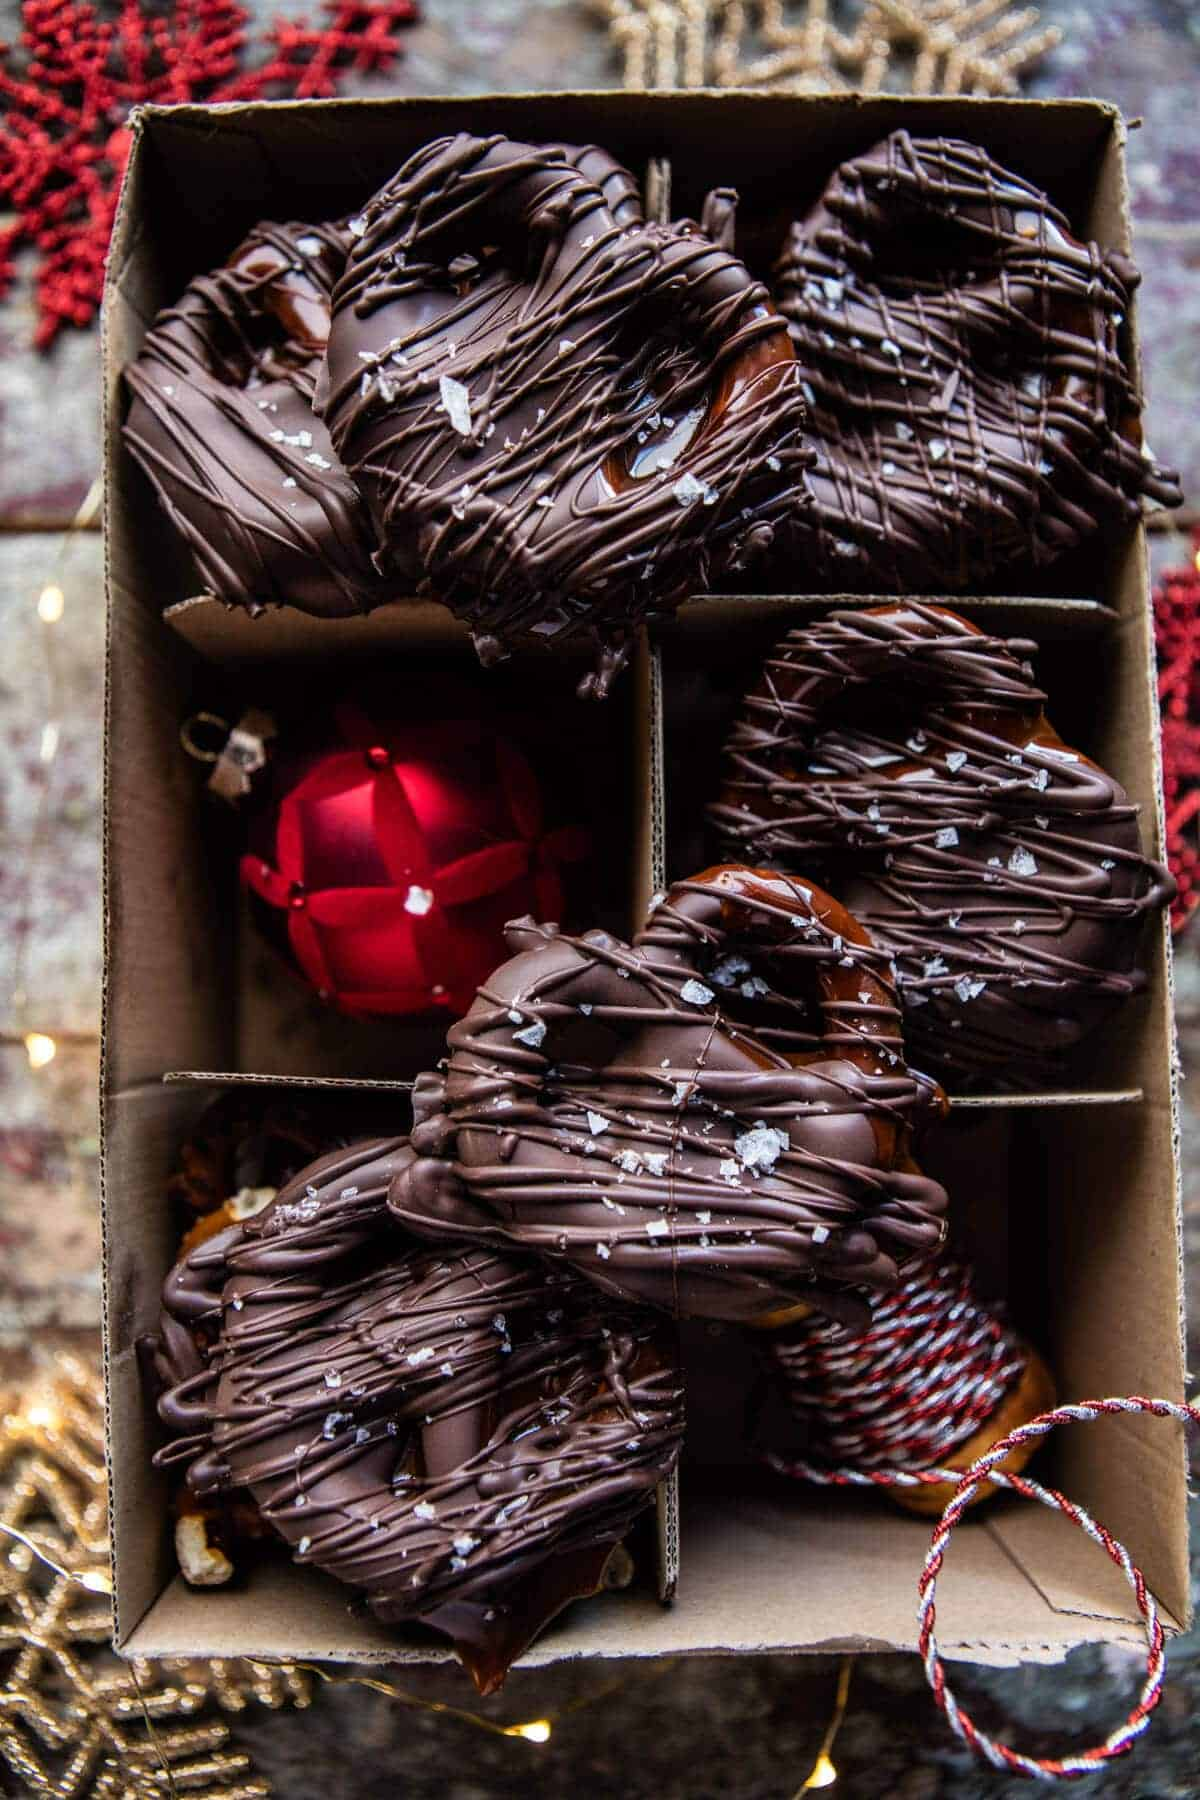
\includegraphics[width=1\textwidth,height=\textheight]{images/salted-caramel-chocolate-covered-pretzels-.jpg}

\textbf{Prep Time:} 20 min \textbar{} \textbf{Cook Time:} \textbar{}
\textbf{Total Time:} 20 min

\section{Ingredients}\label{ingredients-154}

\begin{itemize}
\tightlist
\item
  1 (14 ounce) bag of caramels (unwrapped (or caramel bits))
\item
  1/4 cup heavy cream
\item
  2 teaspoons vanilla extract
\item
  1 (16 ounce) bag of pretzels (use your favorite size/shape)
\item
  12 ounces milk (semi-sweet or dark chocolate, melted)
\item
  flaky sea salt (for topping)
\end{itemize}

\section{Instructions}\label{instructions-154}

\begin{enumerate}
\def\labelenumi{\arabic{enumi}.}
\tightlist
\item
  Line 2 baking sheets with parchment paper.
\item
  Combine the caramels and cream in a saucepan over low heat. Melt
  stirring occasionally, until smooth, about 10 minutes. Remove from the
  heat and stir in the vanilla.
\item
  Dip each pretzel in the caramel and remove with a fork allowing any
  excess to drip off and back into the pan. Place each pretzel on the
  prepared baking sheet and let the caramel set, about 10 minutes.
\item
  Meanwhile, melt the chocolate in a microwave safe bowl on 30 second
  intervals, stirring after each until melted and smooth.
\item
  Dip each pretzel in chocolate and return to the parchment lined baking
  sheets. Repeat with the remaining pretzels. Sprinkle with flaky sea
  salt. Place the pretzels in the freezer to set for 10 minutes. Store
  in an air-tight container for up to 1 week.
\end{enumerate}

\bookmarksetup{startatroot}

\chapter{Mushroom Cheese Ravioli with Rosemary Butter
Sauce.}\label{mushroom-cheese-ravioli-with-rosemary-butter-sauce.}

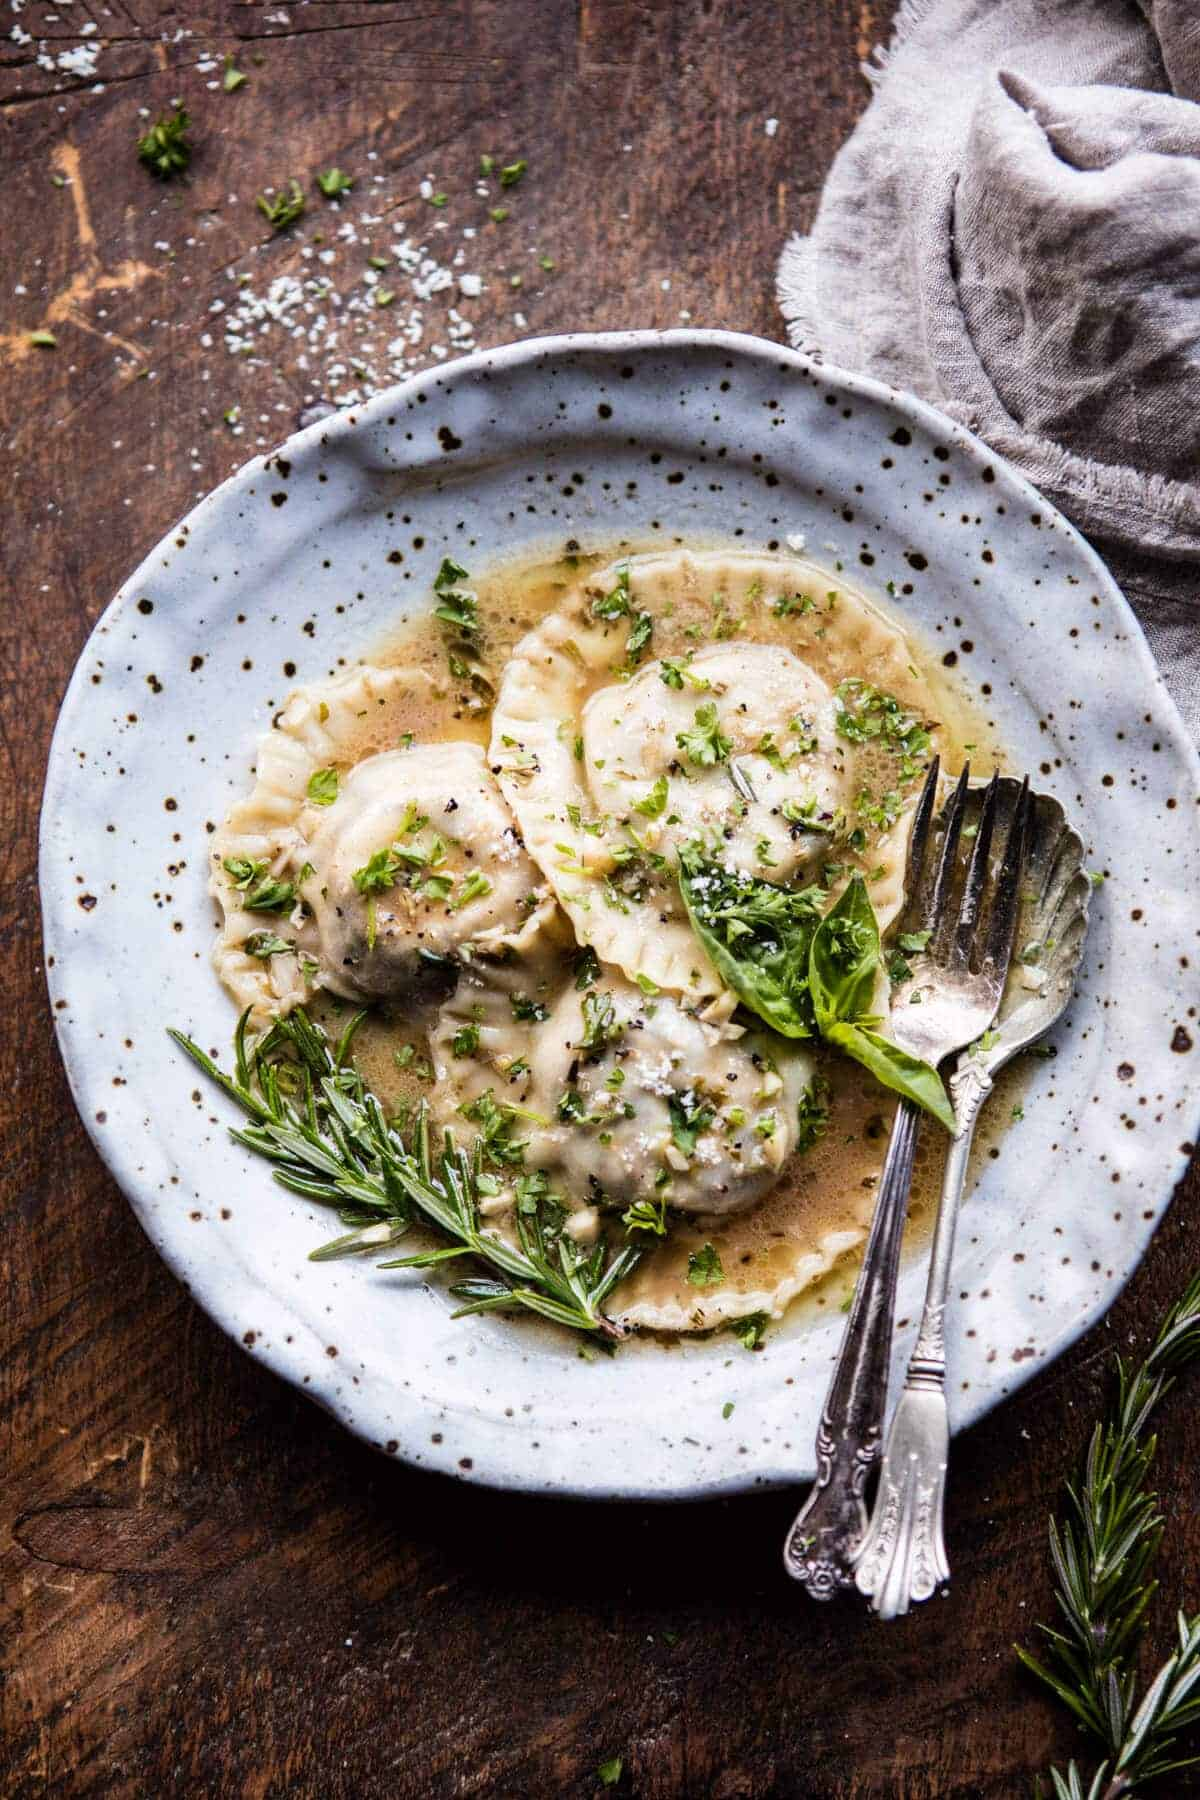
\includegraphics[width=1\textwidth,height=\textheight]{images/mushroom-cheese-ravioli-with-rosemary-butter-sauce-.jpg}

\textbf{Prep Time:} 45 min \textbar{} \textbf{Cook Time:} 15 min
\textbar{} \textbf{Total Time:} 1 hr

\section{Ingredients}\label{ingredients-155}

\begin{itemize}
\tightlist
\item
  2 tablespoons butter
\item
  16 ounces cremini mushrooms (chopped)
\item
  1 tablespoon chopped fresh thyme
\item
  2 tablespoons balsamic vinegar
\item
  1 cup whole milk ricotta cheese
\item
  1 cup shredded fontina cheese
\item
  1/2 cup grated parmesan cheese
\item
  kosher salt + pepper
\item
  40-50 circle or square wonton wrappers
\item
  8 tablespoon salted butter
\item
  3 cloves garlic (minced or grated)
\item
  1 tablespoon chopped fresh rosemary (plus more for serving)
\item
  1/2 cup white wine or chicken broth
\item
  2 cups low sodium chicken broth
\item
  chopped parsley (for serving)
\end{itemize}

\section{Instructions}\label{instructions-155}

\begin{enumerate}
\def\labelenumi{\arabic{enumi}.}
\tightlist
\item
  Melt the butter in a large skillet set over medium high heat. Add the
  mushrooms and cook until soft and caramelized, about 5 minutes. Add
  the thyme and season with salt and pepper. Add the balsamic vinegar
  and cook until the balsamic coats the mushrooms, about 3-4 minutes.
  Remove from the heat and let cool completely.
\item
  In a medium bowl, stir together the ricotta, fontina, and parmesan.
  Season with salt and pepper. Fold in the mushrooms.
\item
  Lay out about 6 wrappers. Spoon 1 tablespoon of filling into the
  center of each wrapper. Brush the edges with water. Lay a second
  wrapper on top of each ravioli. Press down the edges to seal, pressing
  out all the air. Crimp the edges with a fork. Alternately you can
  create triangles with the square wrappers if desired. Be sure to keep
  the ravioli's covered as work work to prevent them from drying out.
\item
  Make the butter sauce. In a large skillet, brown the butter over
  medium heat, stirring often until the butter is golden and toasted.
  Add the rosemary and garlic and cook 30 seconds to a minute or until
  fragrant. Pour in the wine and chicken broth and bring to a boil.
  Season with salt and pepper. Cook 5 minutes or until the sauce has
  reduced slightly.
\item
  Meanwhile, bring a large pot of salted water to a boil. Boil the
  ravioli in batches for 1-2 minutes or until they float. Drain.
\item
  Divide the ravioli among bowls and ladle the sauce over the ravioli.
  Top with parmesan and parsley. EAT!
\end{enumerate}

\bookmarksetup{startatroot}

\chapter{Christmas Ale Sangria.}\label{christmas-ale-sangria.}

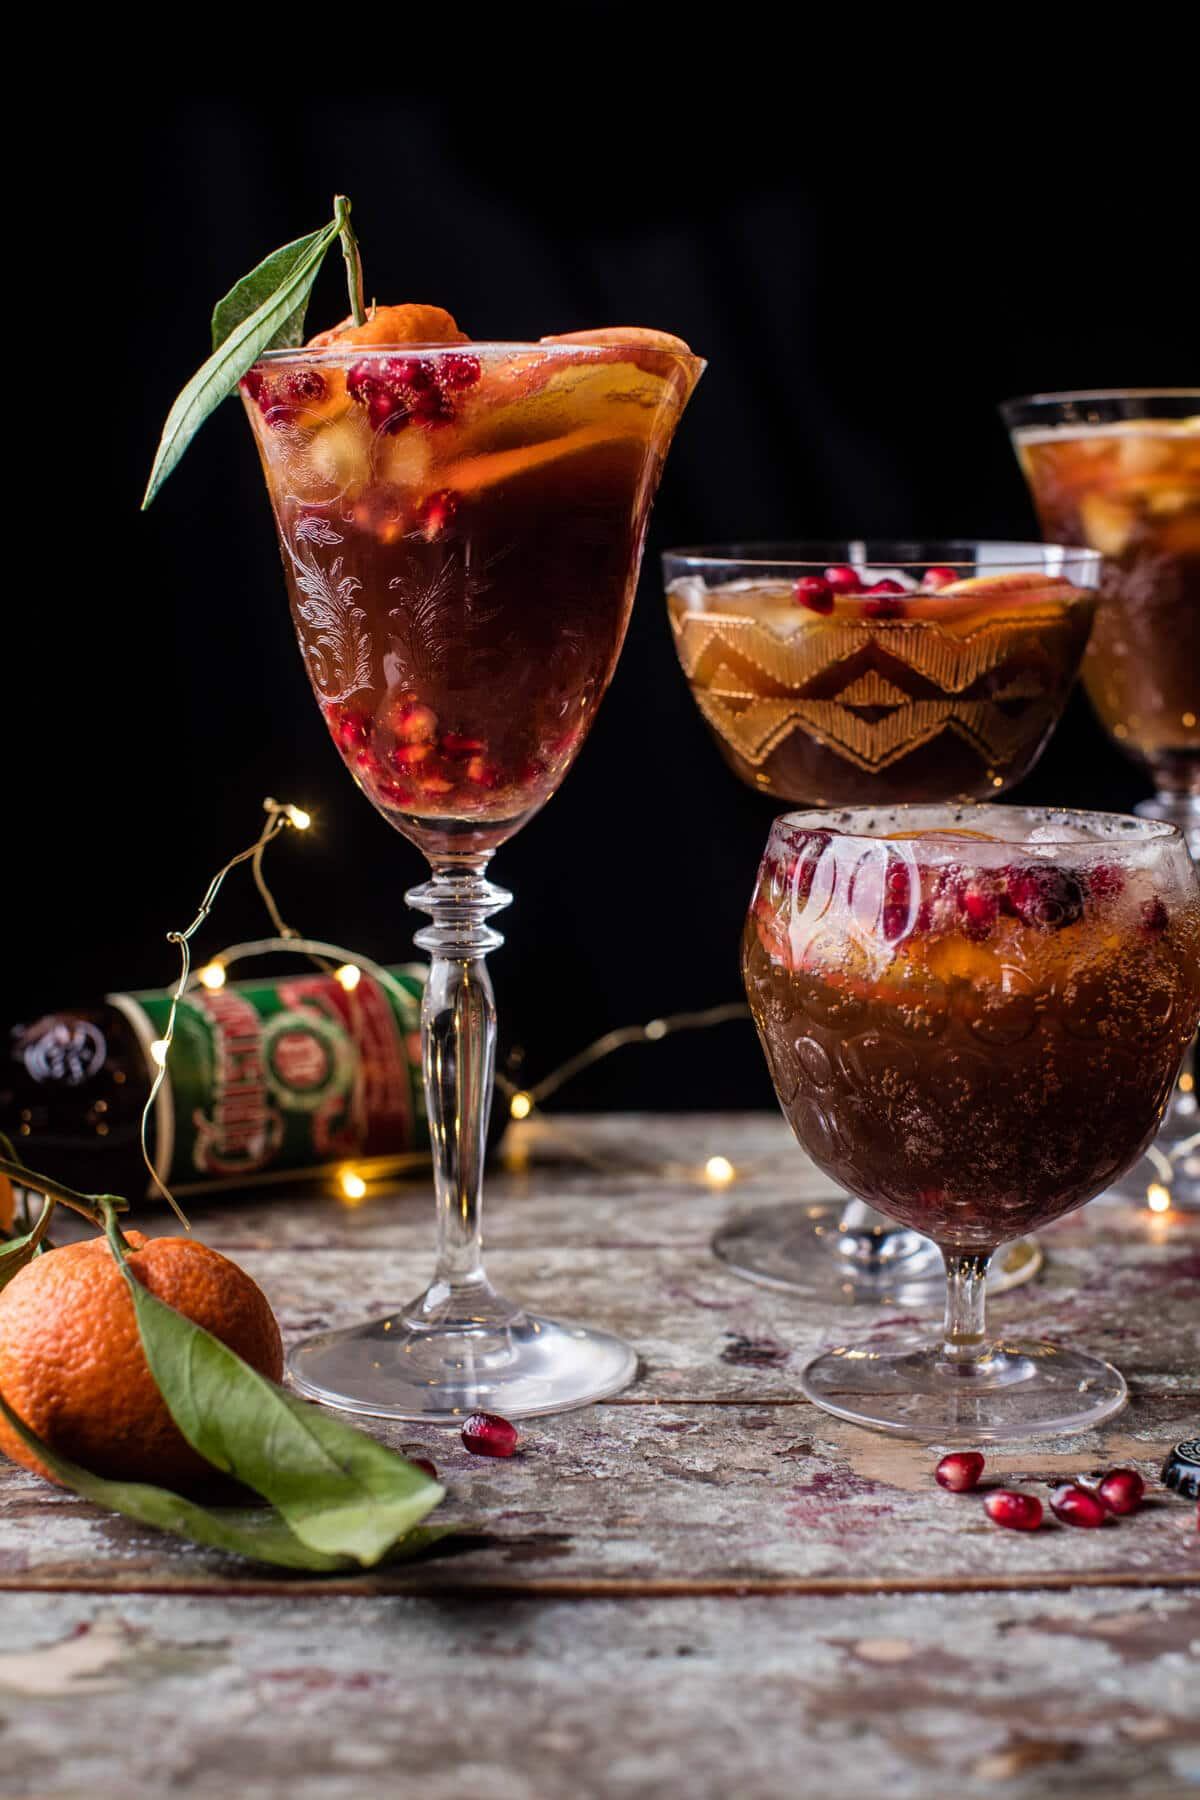
\includegraphics[width=1\textwidth,height=\textheight]{images/christmas-ale-sangria-.jpg}

\textbf{Prep Time:} 10 min \textbar{} \textbf{Cook Time:} \textbar{}
\textbf{Total Time:} 10 min

\section{Ingredients}\label{ingredients-156}

\begin{itemize}
\tightlist
\item
  1 1/2 cups apple cider
\item
  1/2 cup vodka
\item
  6 dashes orange bitters
\item
  2 pears (sliced)
\item
  3 oranges (sliced)
\item
  arils from 1 pomegranate
\item
  1 cup cranberries
\item
  3 cinnamon sticks
\item
  5 bottles Christmas Ale (chilled)
\item
  sparkling water (for topping (optional))
\end{itemize}

\section{Instructions}\label{instructions-156}

\begin{enumerate}
\def\labelenumi{\arabic{enumi}.}
\tightlist
\item
  In a large pitcher, add the apple cider, vodka and orange bitters,
  stir to combine. Add the pears, oranges, pomegranate arils, and
  cranberries. Chill until ready to serve.
\item
  Before serving, slowly pour in the beer and gently stir to combine.
  Pour among glasses and top with sparkling water if desired.
\end{enumerate}

\bookmarksetup{startatroot}

\chapter{Chocolate Peanut Butter Crinkle
Cookies.}\label{chocolate-peanut-butter-crinkle-cookies.}

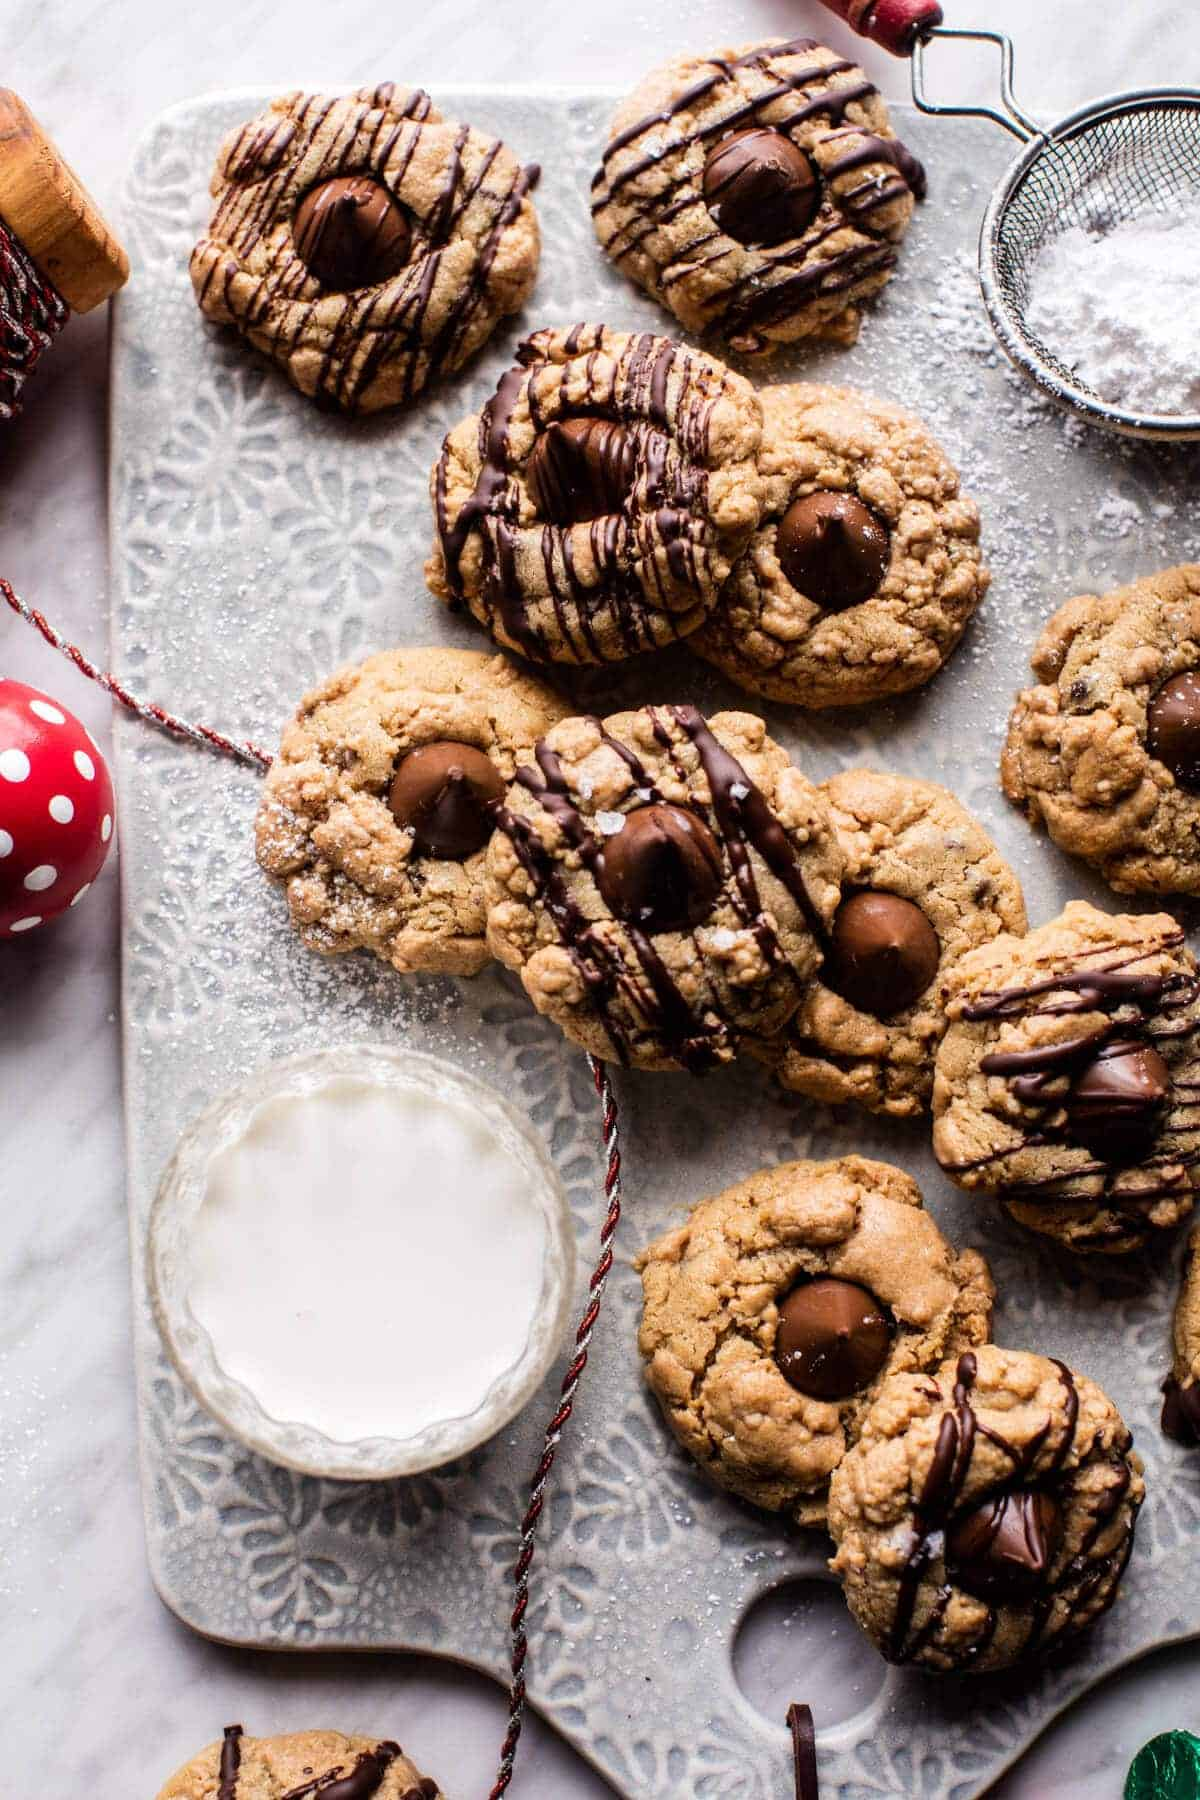
\includegraphics[width=1\textwidth,height=\textheight]{images/chocolate-peanut-butter-crinkle-cookies-.jpg}

\textbf{Prep Time:} 15 min \textbar{} \textbf{Cook Time:} 10 min
\textbar{} \textbf{Total Time:} 25 min

\section{Ingredients}\label{ingredients-157}

\begin{itemize}
\tightlist
\item
  2 sticks butter (at room temperature)
\item
  1 cup creamy peanut butter
\item
  1/2 cup light brown sugar
\item
  1/4 cup granulated sugar
\item
  1 egg
\item
  2 teaspoons vanilla extract
\item
  1 1/3 cups all-purpose flour
\item
  3/4 teaspoon baking soda
\item
  1/2 teaspoon baking powder
\item
  1/4 teaspoons salt
\item
  1/3 cup mini chocolate chips
\item
  2/3 cup powdered sugar
\item
  36-40 chocolate kisses
\end{itemize}

\section{Instructions}\label{instructions-157}

\begin{enumerate}
\def\labelenumi{\arabic{enumi}.}
\tightlist
\item
  Preheat the oven to 350 degrees F. Line two baking sheets with
  parchment paper.
\item
  In a mixing bowl, beat together the butter, 1/2 cup peanut butter,
  brown sugar, and granulated sugar using an electric mixer until smooth
  and creamy. Add the egg and vanilla and beat until combined. Add the
  flour, baking soda, baking powder, and salt and mix until just
  combined. Fold in the mini chocolate chips.
\item
  In a medium bowl, combine the remaining 1/2 cup peanut butter and the
  powdered sugar. The mix will be clumpy and moist. Cover and
  refrigerate 30 minutes or up to 3 days.
\item
  Roll the cookie dough into 2 teaspoon size balls and then roll each
  ball through the peanut butter powdered sugar mix, pressing gently to
  adhere. Place 2-inches apart on the prepared baking sheet. Transfer to
  the oven and bake for 10-12 minutes, until the cookies are just set
  around the edges but still doughy in the center. It's important not to
  overbake these as they will be dry and crumbly. Remove from the oven
  and insert 1 kiss into the center of each cookie. Let the cookies cool
  on the baking sheet for 15 minutes and then transfer to a cooling rack
  to cool completely. If desired, drizzle with melted chocolate and
  sprinkle with sea salt. Let the chocolate set at room temp. Cookies
  can be stored in an airtight container for up to 1 week.
\end{enumerate}

\bookmarksetup{startatroot}

\chapter{Caramelized Balsamic Goat Cheese
Pasta.}\label{caramelized-balsamic-goat-cheese-pasta.}

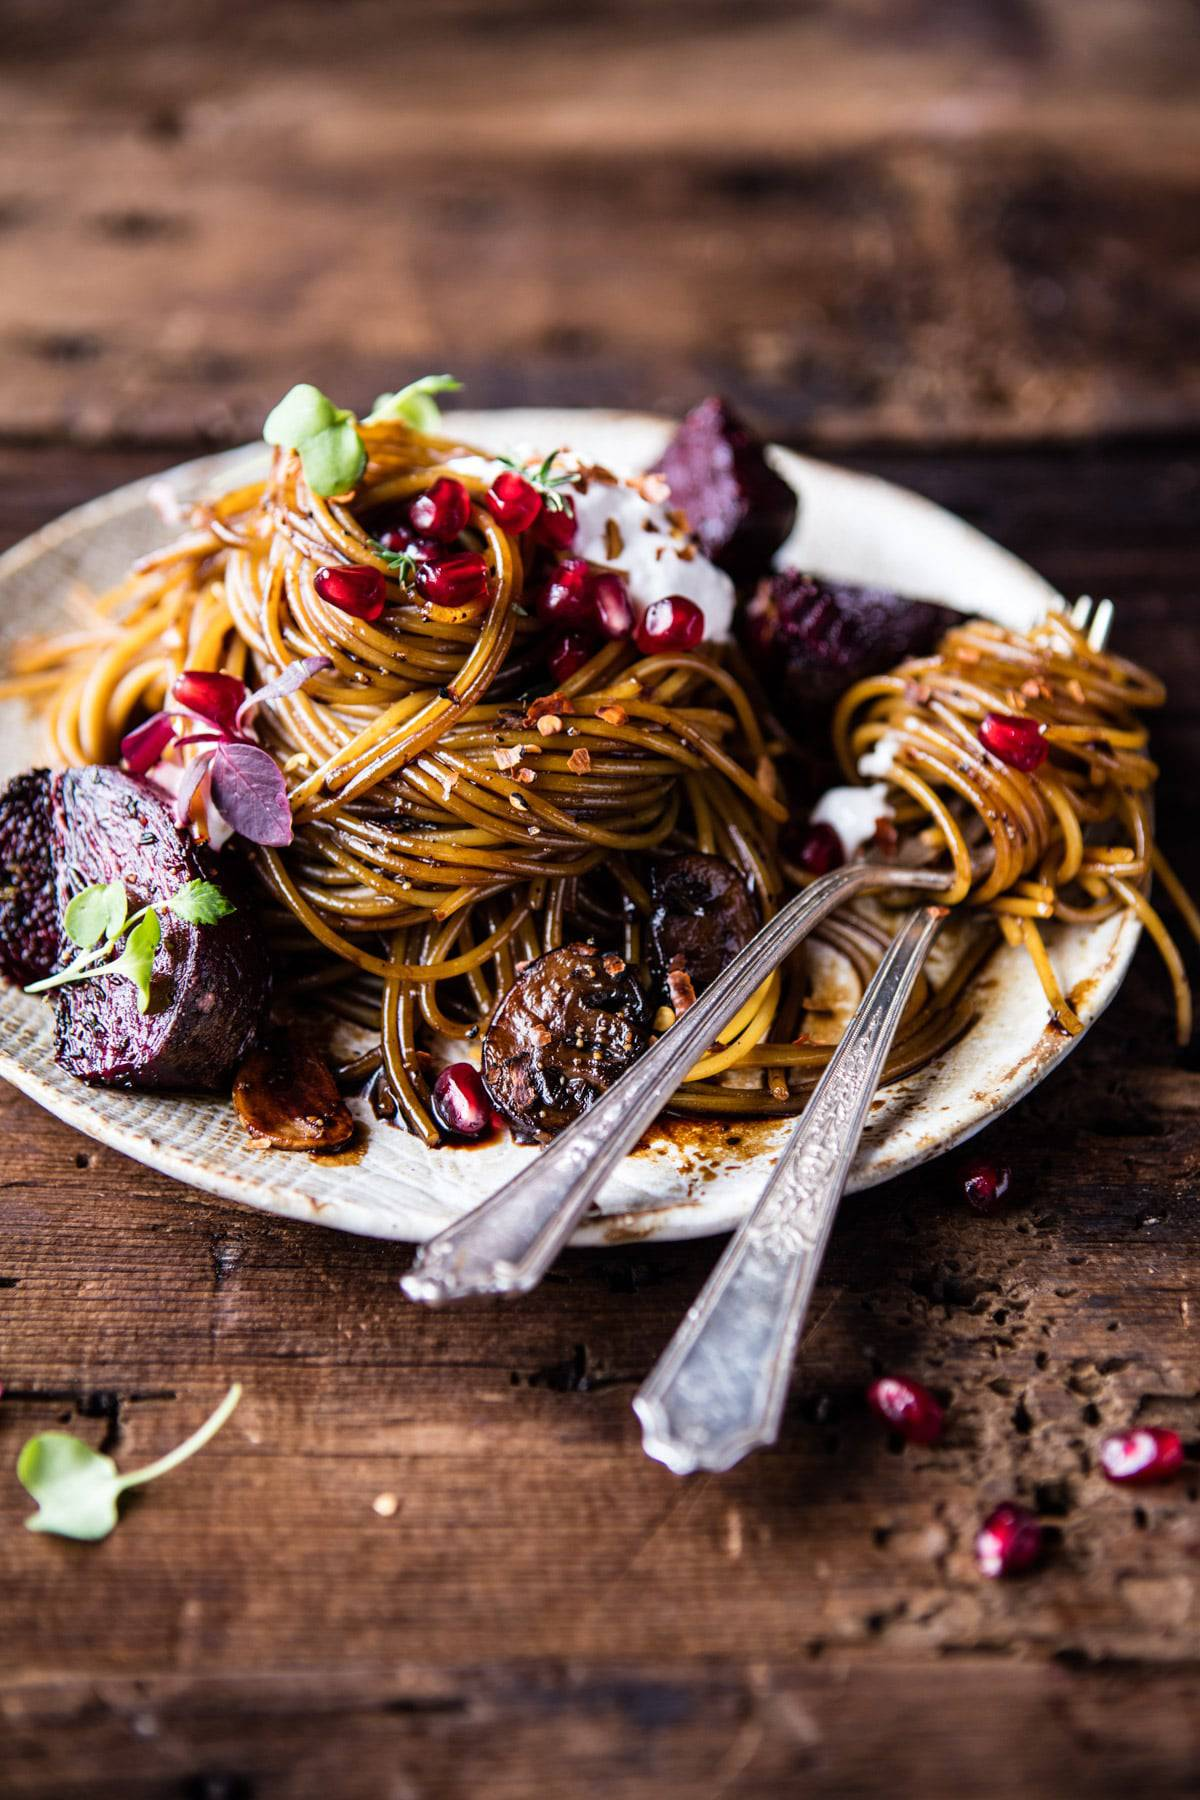
\includegraphics[width=1\textwidth,height=\textheight]{images/caramelized-balsamic-goat-cheese-pasta-.jpg}

\textbf{Prep Time:} 10 min \textbar{} \textbf{Cook Time:} 20 min
\textbar{} \textbf{Total Time:} 30 min

\section{Ingredients}\label{ingredients-158}

\begin{itemize}
\tightlist
\item
  4 tablespoons olive oil
\item
  4 medium red beets, quartered
\item
  1 tablespoon chopped fresh thyme
\item
  kosher salt and pepper
\item
  1 pound long cut pasta, such as spaghetti
\item
  2 tablespoons butter
\item
  8 ounces cremini mushrooms, sliced
\item
  4 cloves garlic, thinly sliced
\item
  1 cup balsamic vinegar
\item
  2-3 tablespoons honey
\item
  1/2 teaspoon crushed red pepper flakes
\item
  1/2 cup crumbled goat cheese or whipped goat cheese
\item
  pomegranate arils, for serving (optional)
\end{itemize}

\section{Instructions}\label{instructions-158}

\begin{enumerate}
\def\labelenumi{\arabic{enumi}.}
\tightlist
\item
  Preheat the oven to 425 degrees F.
\item
  On a baking sheet, toss together 2 tablespoons olive oil, the beets,
  thyme, and a good pinch of salt + pepper. Transfer to the oven and
  roast for 25-30 minutes or until the beets are tender and lightly
  charred.
\item
  Meanwhile, bring a large pot of salted water to a boil. Boil the pasta
  until al dente according to package directions. Just before draining,
  reserve 1 cup of the pasta cooking water. Drain.
\item
  Melt the butter and 2 tablespoons olive oil in a large skillet over
  high heat. Add the mushrooms and cook until they just begin to
  caramelize on the edges, about 5 minutes. Add the garlic and cook 30
  seconds to 1 minute or until fragrant. Remove the mushrooms and garlic
  from the skillet and place on a plate. To the same skillet, add the
  balsamic vinegar, honey and crushed red pepper flakes. Bring to a boil
  over medium high heat and cook for 5-8 minutes or until the balsamic
  reduces by about 1/3 and is sticky to touch. Reduce the heat to low
  and stir in the pasta and mushrooms. Toss to coat, if the sauce seems
  too thick, thin it with a little of the pasta cooking water. Season to
  taste with salt and pepper.
\item
  Serve the pasta immediately, topped with roasted beets, goat cheese,
  and pomegranate arils (if using). Eat!
\end{enumerate}

\bookmarksetup{startatroot}

\chapter{Cheesy Sweet and Sour Pomegranate Thai Chicken
Enchiladas}\label{cheesy-sweet-and-sour-pomegranate-thai-chicken-enchiladas}

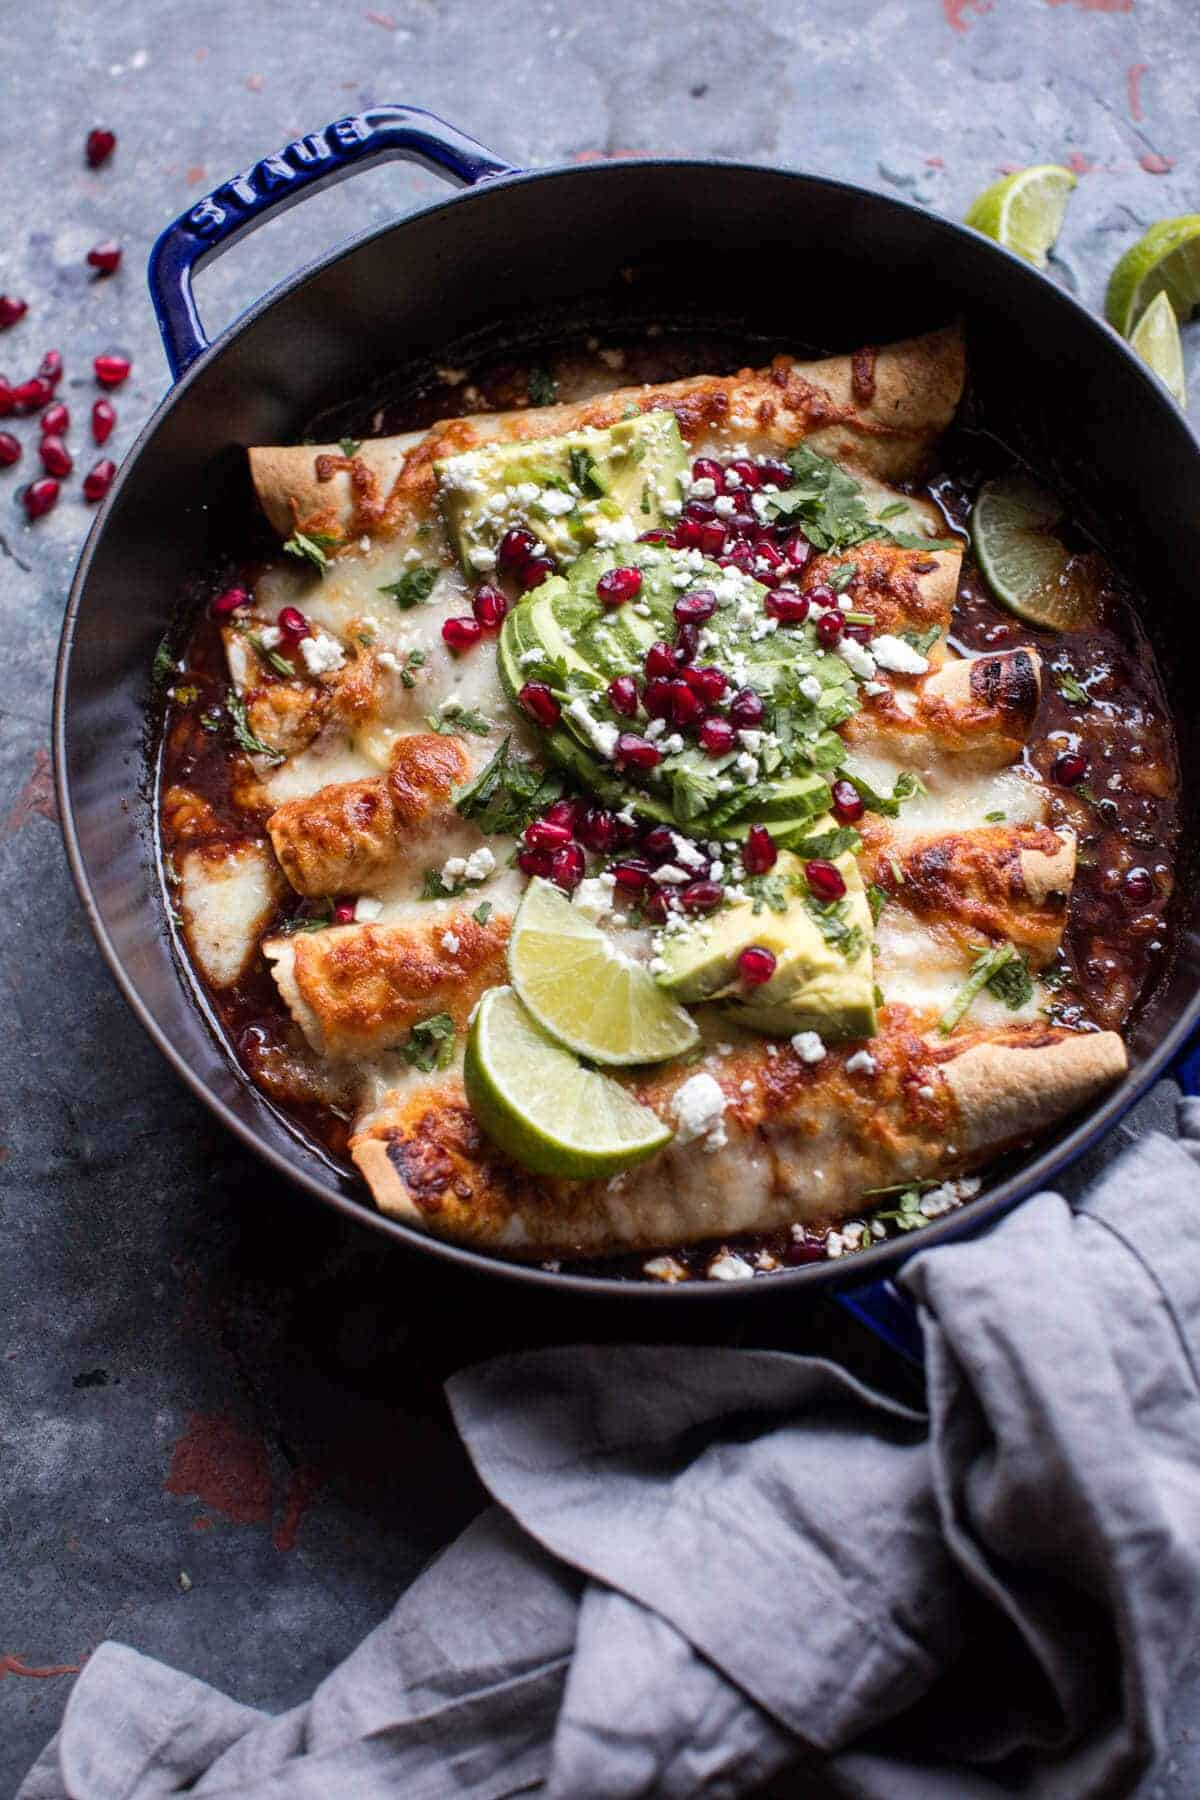
\includegraphics[width=1\textwidth,height=\textheight]{images/cheesy-sweet-and-sour-pomegranate-thai-chicken-enchiladas.jpg}

\textbf{Prep Time:} 20 min \textbar{} \textbf{Cook Time:} 40 min
\textbar{} \textbf{Total Time:} 1 hr

\section{Ingredients}\label{ingredients-159}

\begin{itemize}
\tightlist
\item
  1 1/2 cups sweet thai chili sauce
\item
  1/2 cup soy sauce
\item
  1/3 cup dark brown sugar
\item
  1 tablespoon peanut butter
\item
  1 tablespoon tomato paste
\item
  3/4 cup pomegranate juice
\item
  1/4 cup rice vinegar
\item
  Juice of 1 lime
\item
  1 teaspoon fish sauce (optional)
\item
  2 cloves garlic (minced or grated)
\item
  1 inch fresh ginger (grated)
\item
  2 cooked chicken breasts, shredded ((about 2 cups))
\item
  2 red or orange bell peppers (sliced thin)
\item
  1 1/2 cups shredded mozzarella cheese
\item
  10 Old El Paso Flour Tortillas
\item
  Sliced avocado, pomegranate arils, and chopped cilantro, for serving
\end{itemize}

\section{Instructions}\label{instructions-159}

\begin{enumerate}
\def\labelenumi{\arabic{enumi}.}
\tightlist
\item
  Preheat the oven to 350 degrees F. Grease a 9x13-inch baking dish.
\item
  To make the sauce. Combine the sweet thai chili sauce, soy sauce, dark
  brown sugar, peanut butter, tomato paste, pomegranate juice, rice
  vinegar, lime juice, fish sauce, garlic, and ginger in a medium sauce
  pan. Bring the sauce to a boil, reduce the heat and simmer 10-15
  minutes or until sauce has thickened slightly. Remove from the heat
  and set aside.
\item
  To a medium bowl, add the shredded chicken, sliced bell pepper,
  cilantro and 1/2 cup shredded mozzarella. Pour in about 3/4 cup of the
  sauce or just enough to coat the chicken and make it saucy. Toss to
  coat.
\item
  Wrap the tortillas in a damp paper towel and microwave for one minute.
  Spoon a little of the chicken mixture down the center of each
  tortilla, tuck and roll, placing the tortilla, seam side down, into
  the baking dish. Pour the remaining sauce over top of the enchiladas
  and then top with the remaining 1 cup mozzarella. Transfer to the oven
  and bake for 30 minutes, until the cheese has melted. Remove and top
  with diced avocado and pomegranate arils.
\end{enumerate}

\bookmarksetup{startatroot}

\chapter{Sugar Cookie Hot Chocolate.}\label{sugar-cookie-hot-chocolate.}


\includegraphics[width=1\textwidth,height=\textheight]{images/sugar-cookie-hot-chocolate-.jpg}

\textbf{Prep Time:} 10 min \textbar{} \textbf{Cook Time:} 10 min
\textbar{} \textbf{Total Time:} 20 min

\section{Ingredients}\label{ingredients-160}

\begin{itemize}
\tightlist
\item
  4 1/2 cups whole milk
\item
  2/3 cup sweetened condensed milk
\item
  1/4 cup cocoa powder
\item
  6 ounces semi-sweet or dark chocolate (chopped)
\item
  1 tablespoon vanilla extract
\item
  1/4 teaspoon almond extract
\item
  whipped cream (marshmallows, sugar cookies and or coarse sugar, for
  topping)
\end{itemize}

\section{Instructions}\label{instructions-160}

\begin{enumerate}
\def\labelenumi{\arabic{enumi}.}
\tightlist
\item
  Add the milk, sweetened condensed milk, cocoa powder, chocolate,
  vanilla, and almond extract (if using) to a large pot. Place the pot
  over medium low heat until the milk is scalding, but not boiling. Be
  sure to stir the pot often to make sure nothing is sticking to the
  bottom and burning.
\item
  Once the hot chocolate is steaming, ladle into mugs and dollop with
  whipped cream. Add marshmallows, cookies and a sprinkle of sugar if
  desired. Drink!
\end{enumerate}

\bookmarksetup{startatroot}

\chapter{Cheese Fondue Board.}\label{cheese-fondue-board.}

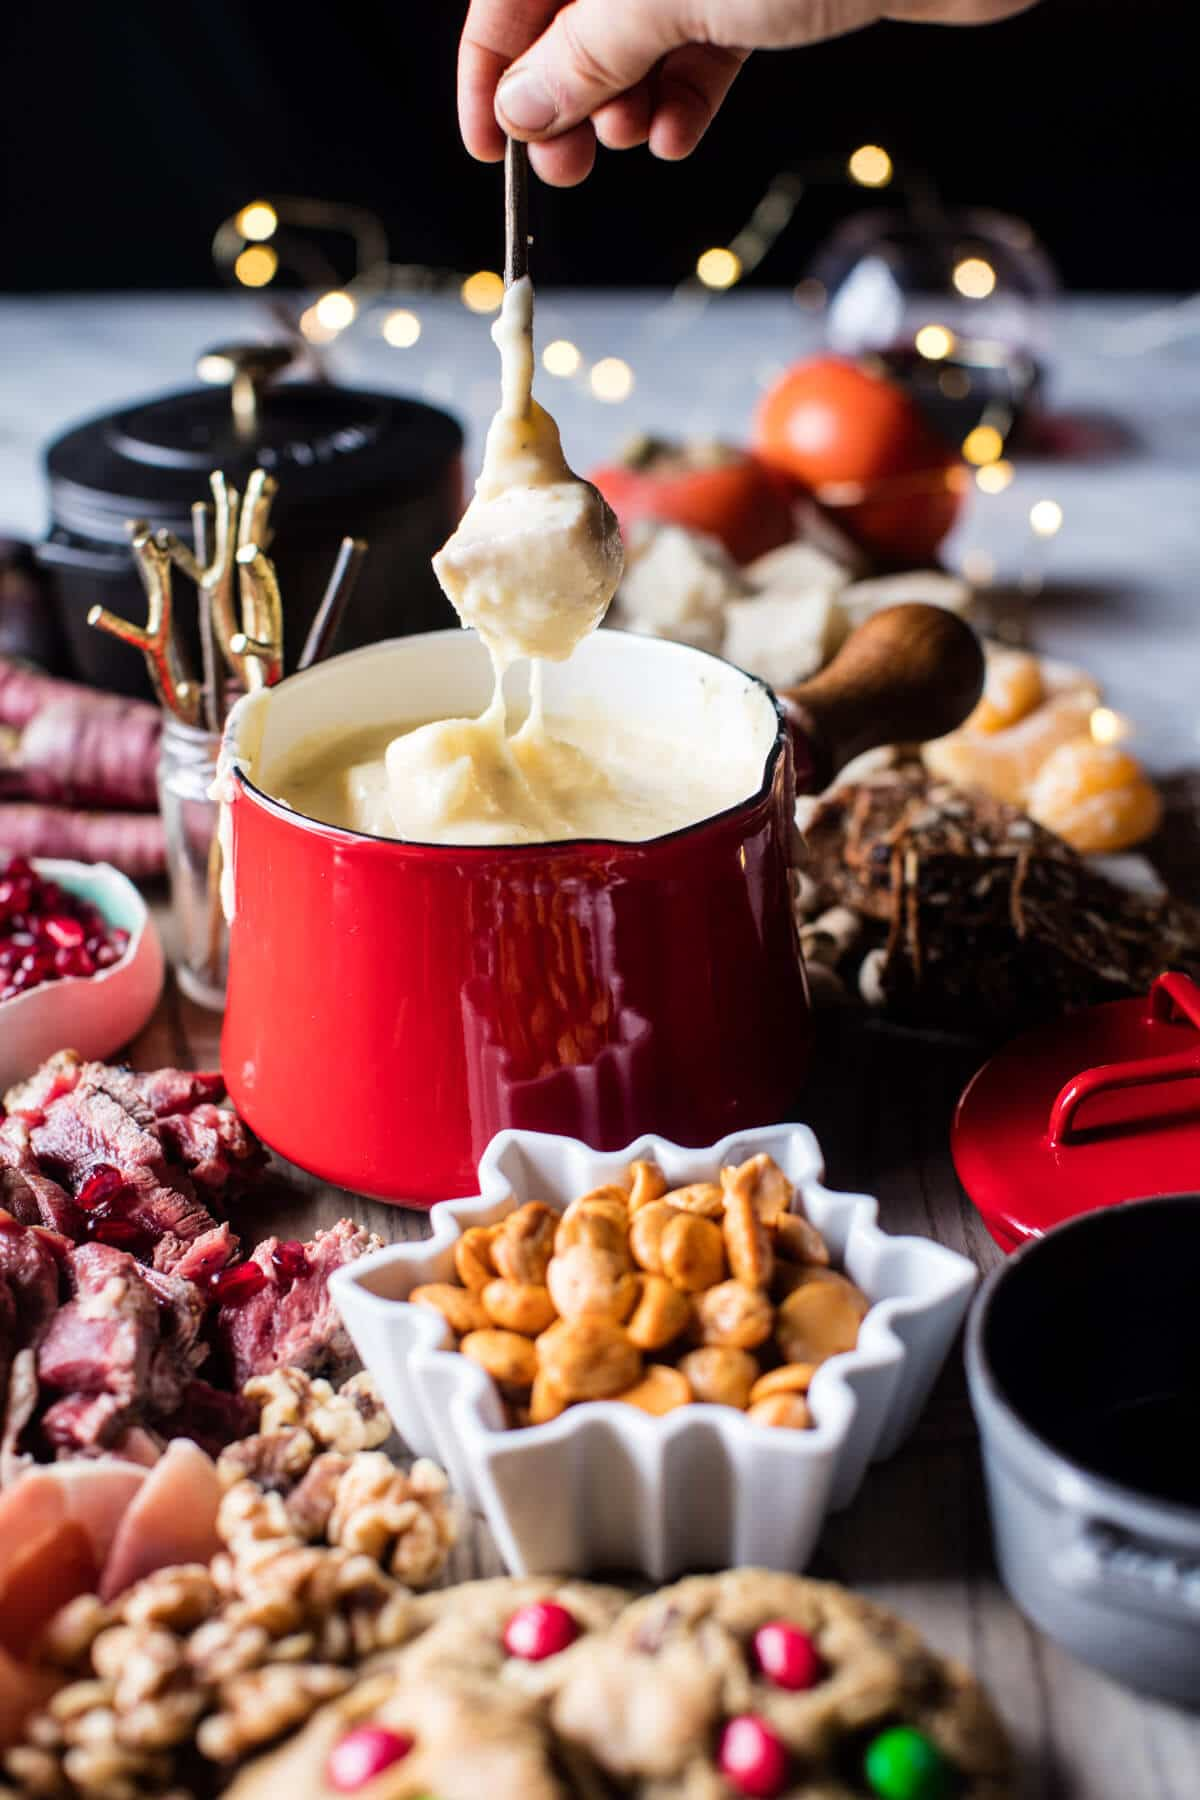
\includegraphics[width=1\textwidth,height=\textheight]{images/cheese-fondue-board-.jpg}

\textbf{Prep Time:} 15 min \textbar{} \textbf{Cook Time:} 15 min
\textbar{} \textbf{Total Time:} 30 min

\section{Ingredients}\label{ingredients-161}

\begin{itemize}
\tightlist
\item
  3 cups shredded swiss cheese
\item
  3 cups shredded gruyere cheese
\item
  2 tablespoons cornstarch
\item
  1 clove garlic
\item
  1 cup white wine (may use chicken broth)
\item
  pinch of freshly grated nutmeg
\item
  kosher salt + pepper
\item
  3 cups shredded cheddar
\item
  3 cups shredded aged gouda
\item
  2 tablespoons cornstarch
\item
  1 clove garlic
\item
  1 cup beer (may use chicken broth)
\item
  1/4 teaspoon mustard powder
\item
  4 ounces crumbled blue cheese (optional)
\item
  kosher salt + pepper
\item
  assorted crackers and breads
\item
  assort winter fruits and vegetables
\item
  thinly sliced grilled steak and or assorted deli meats
\item
  honey and or honeycomb
\item
  toasted nuts (I love marcona almonds (walnuts, and pistachios))
\end{itemize}

\section{Instructions}\label{instructions-161}

\begin{enumerate}
\def\labelenumi{\arabic{enumi}.}
\tightlist
\item
\end{enumerate}

\bookmarksetup{startatroot}

\chapter{Crockpot Sun-Dried Tomato Penne Alla
Vodka.}\label{crockpot-sun-dried-tomato-penne-alla-vodka.}

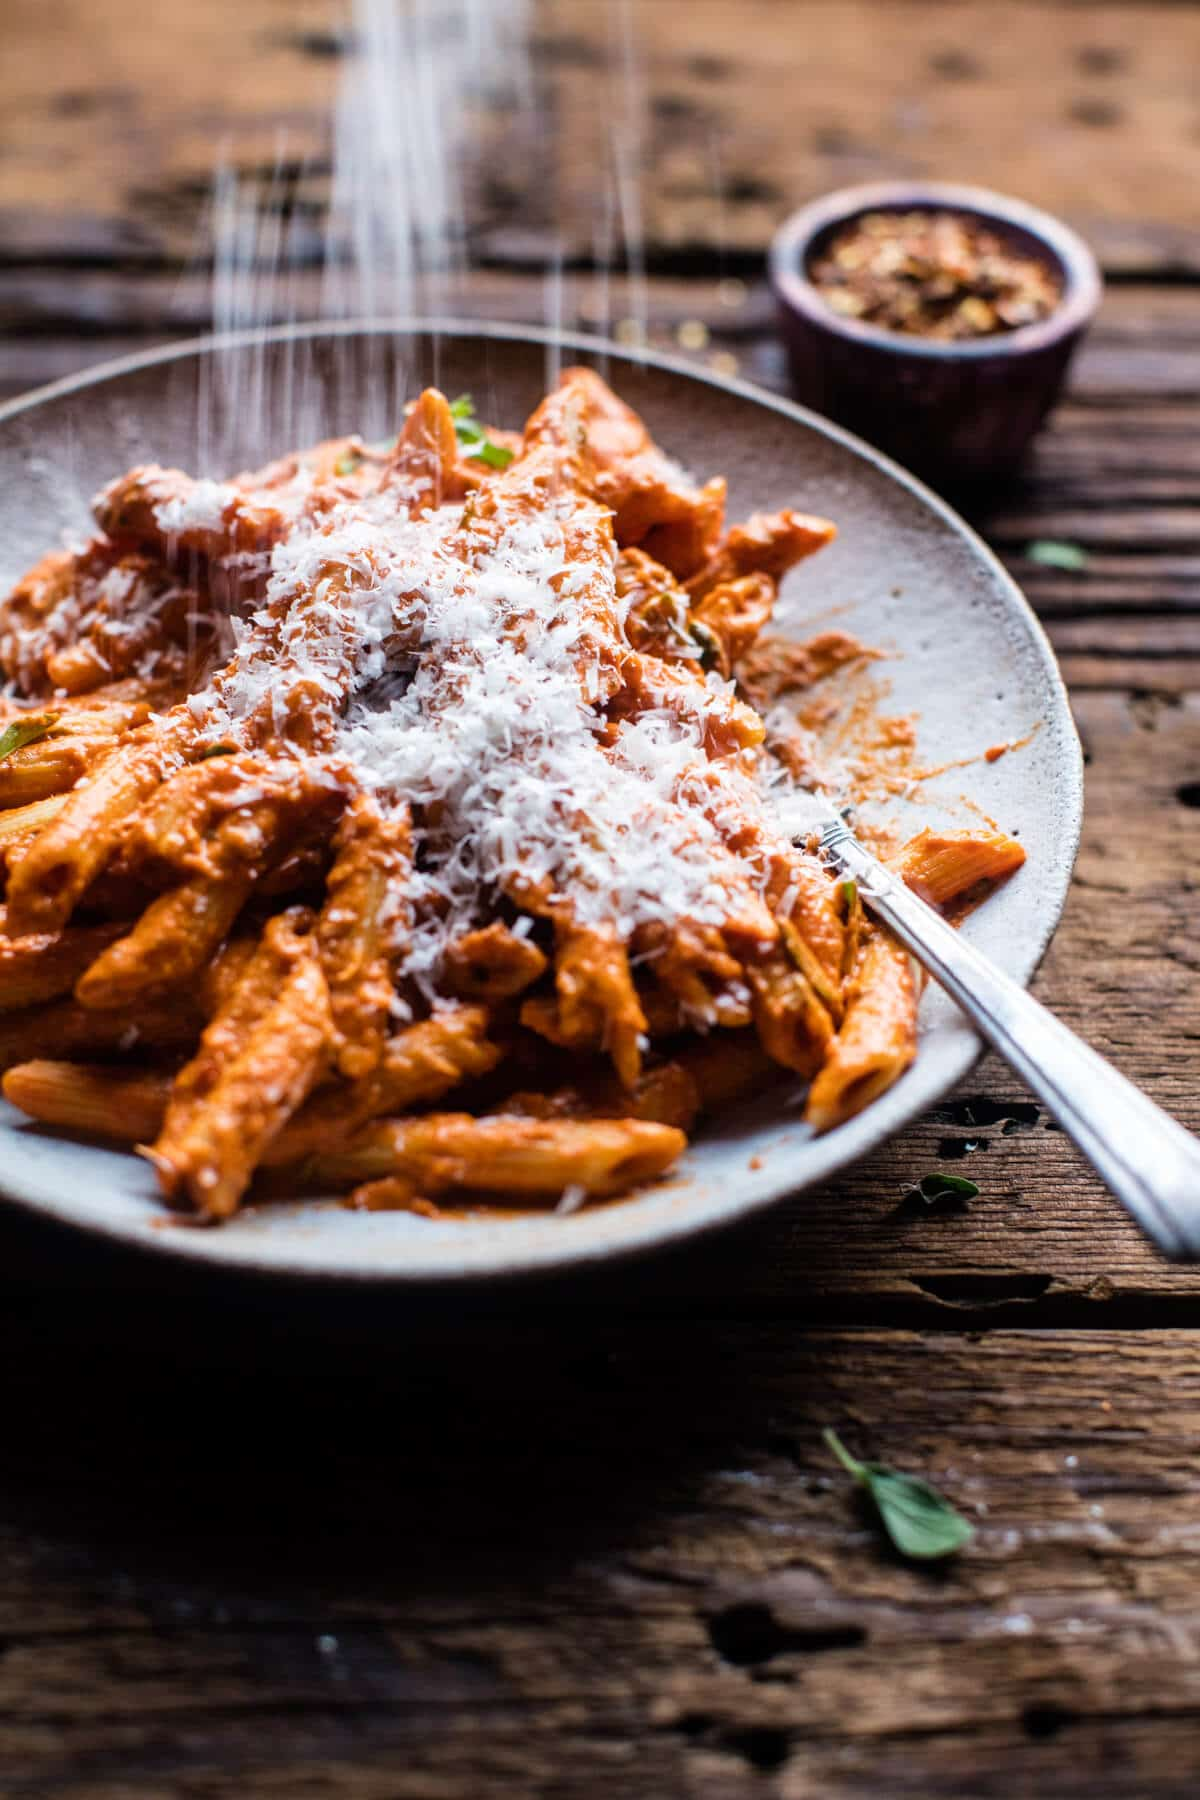
\includegraphics[width=1\textwidth,height=\textheight]{images/crockpot-sun-dried-tomato-penne-alla-vodka-.jpg}

\textbf{Prep Time:} 15 min \textbar{} \textbf{Cook Time:} 6 hr
\textbar{} \textbf{Total Time:} 6 hr 15 min

\section{Ingredients}\label{ingredients-162}

\begin{itemize}
\tightlist
\item
  1/4 cup olive oil
\item
  1 sweet onion (diced)
\item
  4 cloves garlic (minced or grated)
\item
  1/2 teaspoon crushed red pepper flakes
\item
  1 1/2 teaspoons dried oregano
\item
  1 cup vodka
\item
  2 (28 ounce) cans whole tomatoes (I like San Marzano)
\item
  1/2 cup oil packed sun-dried tomatoes (drained (see note))
\item
  kosher salt and pepper
\item
  1 cup heavy cream
\item
  1 cup grated parmesan cheese
\item
  1 pound penne pasta
\item
  4 tablespoons chopped fresh oregano
\end{itemize}

\section{Instructions}\label{instructions-162}

\begin{enumerate}
\def\labelenumi{\arabic{enumi}.}
\tightlist
\item
  Heat the olive oil, onion, garlic, crushed red pepper, and dried
  oregano in a large skillet over medium low heat. Cook, stirring often
  until the onion is soft and the garlic fragrant, about 10 minutes. Add
  the vodka, raise the heat, and bring the mixture to a boil, boil 5
  minutes. Remove from the heat and add to the bowl of your crockpot
  along with the tomatoes, sun-dried tomatoes and large pinch of salt +
  pepper. Cover and cook on low for 6-8 hours or on high for 4-5 hours.
  Transfer the sauce to a blender and puree until smooth. Return to the
  crockpot and stir in the the cream and the parmesan. Cook uncovered on
  high for 10 minutes.
\item
  Meanwhile, bring a large pot of salted water to a boil and boil the
  pasta until al dente according to package directions. Drain.
\item
  Divide the pasta among plates and top with the sauce, fresh oregano
  and grated parmesan. Eat!
\end{enumerate}

\bookmarksetup{startatroot}

\chapter{Chocolate Espresso Thumbprint
Cookies.}\label{chocolate-espresso-thumbprint-cookies.}


\includegraphics[width=1\textwidth,height=\textheight]{images/chocolate-espresso-thumbprint-cookies-.jpg}

\textbf{Prep Time:} 15 min \textbar{} \textbf{Cook Time:} 8 min
\textbar{} \textbf{Total Time:} 25 min

\section{Ingredients}\label{ingredients-163}

\begin{itemize}
\tightlist
\item
  2 sticks (1 cup) unsalted butter (softened)
\item
  1 cup granulated sugar
\item
  1 egg
\item
  2 teaspoons vanilla extract
\item
  1 tablespoon instant espresso powder
\item
  2 cups all-purpose flour
\item
  1/2 cup unsweetened cocoa powder
\item
  1 1/2 teaspoons kosher salt
\item
  1-2 tablespoons heavy cream (optional)
\item
  8 ounces semi-sweet or dark chocolate (chopped)
\item
  1/3 cup heavy cream
\item
  1 teaspoon vanilla extract
\item
  1-2 teaspoons instant espresso powder
\end{itemize}

\section{Instructions}\label{instructions-163}

\begin{enumerate}
\def\labelenumi{\arabic{enumi}.}
\tightlist
\item
  Preheat the oven to 350 degrees F. Line a baking sheet with parchment
  paper.
\item
  In a large bowl using an electric mixer, beat together the butter and
  sugar until light and fluffy. Add the egg, vanilla, and coffee powder
  and beat until incorporated. Add the flour, cocoa powder, and salt,
  beating until just combined. If the dough feels dry, add 1 tablespoon
  heavy cream.
\item
  Roll the dough into 2 teaspoon size balls and place 1 inch apart on
  the prepared baking sheet. Using the end of a wooden spoon or your
  thumb, press gently in the center of each to create an indentation.
\item
  Transfer to the oven and bake, rotating sheets halfway through, until
  cookies are just set, about 7-8 minutes. If the indentations lose
  their definition, gently press the centers in again. Cool slightly on
  baking sheet and then transfer cookies to wire racks, and let cool
  completely.
\item
  Meanwhile, in a microwave safe bowl, combine the chocolate and cream.
  Microwave on 30 second intervals until melted and smooth. Stir in the
  vanilla and coffee powder until dissolved. Spoon the ganache into the
  center of each cookie. Decorate as desired with sprinkles or edible
  gold leaf. Keep cookies stored in an airtight container for up to 1
  week.
\end{enumerate}

\bookmarksetup{startatroot}

\chapter{Poinsettia Spritz Punch.}\label{poinsettia-spritz-punch.}


\includegraphics[width=1\textwidth,height=\textheight]{images/poinsettia-spritz-punch-.jpg}

\textbf{Prep Time:} 10 min \textbar{} \textbf{Cook Time:} \textbar{}
\textbf{Total Time:} 10 min

\section{Ingredients}\label{ingredients-164}

\begin{itemize}
\tightlist
\item
  3/4 cup vodka
\item
  1 1/2 cups 100\% cranberry juice or pomegranate juice
\item
  2 ounces St.~Germain (elderflower liquor)
\item
  3/4 cup champagne
\item
  1 cup fresh cranberries
\item
  slices rosemary and orange (for serving)
\end{itemize}

\section{Instructions}\label{instructions-164}

\begin{enumerate}
\def\labelenumi{\arabic{enumi}.}
\tightlist
\item
  In a large pitcher, combine the vodka, cranberry juice and
  St.~Germain. Chill until ready to serve.
\item
  When ready to serve, add the champagne and cranberries. Pour among
  glasses and garnish with rosemary and orange zest/slices.
\end{enumerate}

\bookmarksetup{startatroot}

\chapter{Spaghetti and Meatballs.}\label{spaghetti-and-meatballs.}

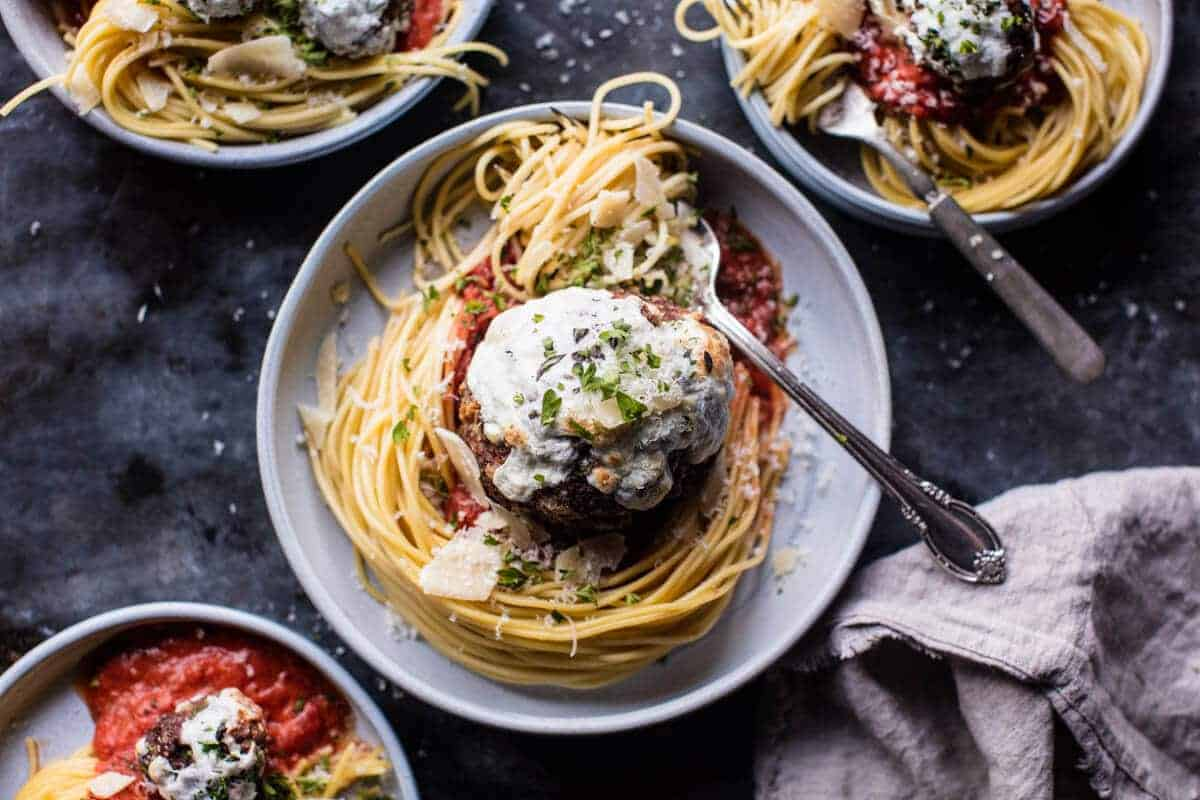
\includegraphics[width=1\textwidth,height=\textheight]{images/spaghetti-and-meatballs-.jpg}

\textbf{Prep Time:} 15 min \textbar{} \textbf{Cook Time:} 30 min
\textbar{} \textbf{Total Time:} 45 min

\section{Ingredients}\label{ingredients-165}

\begin{itemize}
\tightlist
\item
  1 pound lean ground sirloin
\item
  3/4 cup bread crumbs
\item
  1/4 cup grated parmesan cheese
\item
  1/4 cup chopped parsley
\item
  1 teaspoon dried oregano
\item
  pinch of crushed red pepper flakes
\item
  kosher salt and pepper
\item
  2 tablespoons olive oil
\item
  1 egg
\item
  1 jar marinara sauce
\item
  1/3 cup mozzarella (shredded)
\item
  whole wheat pasta or spaghetti squash (for serving)
\end{itemize}

\section{Instructions}\label{instructions-165}

\begin{enumerate}
\def\labelenumi{\arabic{enumi}.}
\tightlist
\item
  Preheat the oven to 450 degrees F. Grease a 9x13 inch baking dish with
  olive oil.
\item
  Mix together the ground sirloin, bread crumbs, parmesan cheese,
  parsley, dried oregano, crushed red pepper, salt, pepper, olive oil
  and egg to a mixing bowl until just combined.
\item
  Coat your hands with a bit of olive oil, and roll the meat into 2
  tablespoon size balls (will make 10-12 meatballs). Place the meatballs
  in the prepared baking dish and place in the oven. Bake for 15 minutes
  or until the meatballs are crisp on the outside, but not yet cooked
  through on the inside. Add the mozzarella cheese and continue cooking
  another 15-20 minutes or until the meatballs are cooked through.
\item
  To make a Giant meatball, form the meat mixture into and oval and
  place in the prepared baking dish. Transfer to the oven and bake for
  35-45 minutes or until the meat is cooked through. During the last 10
  minutes of cooking, add the cheese. Serve with pasta and marinara.
\end{enumerate}

\bookmarksetup{startatroot}

\chapter{Chocolate Dipped Coconut Caramel
Macaroons.}\label{chocolate-dipped-coconut-caramel-macaroons.}

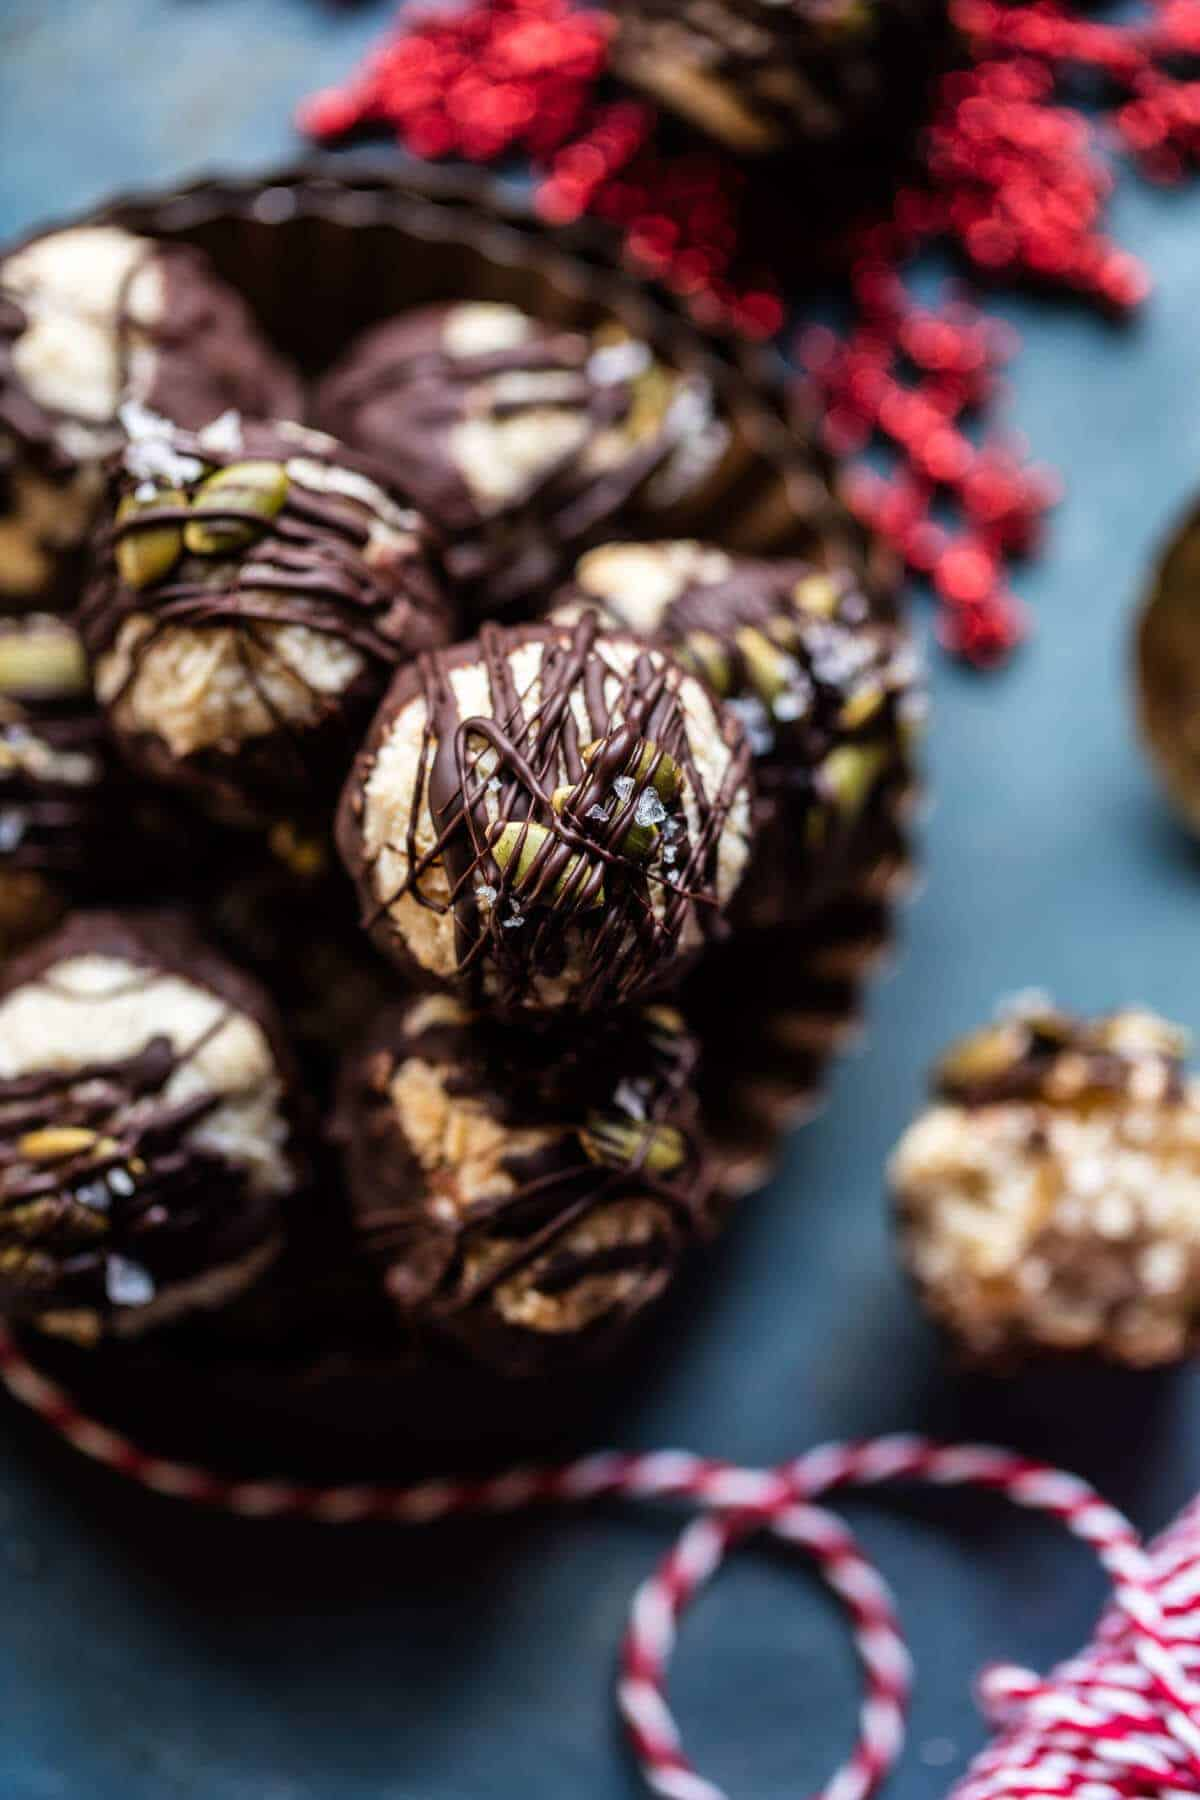
\includegraphics[width=1\textwidth,height=\textheight]{images/chocolate-dipped-coconut-caramel-macaroons-.jpg}

\textbf{Prep Time:} 15 min \textbar{} \textbf{Cook Time:} 15 min
\textbar{} \textbf{Total Time:}

\section{Ingredients}\label{ingredients-166}

\begin{itemize}
\tightlist
\item
  2 tablespoons Bob’s Red Mill Pumpkin Seeds
\item
  3/4 cup maple syrup
\item
  1/4 cup full fat canned coconut milk
\item
  1 tablespoon coconut oil
\item
  2 teaspoons vanilla extract
\item
  pinch of flaky sea salt
\item
  3 cups Bob’s Red Mill Flaked Coconut
\item
  1/2 cup Bob’s Red Mill Almond Flour
\item
  5 ounces dark chocolate (melted)
\end{itemize}

\section{Instructions}\label{instructions-166}

\begin{enumerate}
\def\labelenumi{\arabic{enumi}.}
\tightlist
\item
  Preheat the oven to 350 degrees F. Line two baking sheets with
  parchment paper.
\item
  Add the pumpkin seeds to a prepared baking sheet and place in the oven
  for 5-8 minutes or until lightly toasted. Set aside.
\item
  To make the caramel - In a small saucepan set over medium heat,
  combine the maple syrup, coconut milk and coconut oil. Bring the
  mixture to a boil, stirring continuously, for 10 minutes or until the
  mixture has thickened slightly and reduced to ¾ cup. The caramel
  should be easily pourable. Remove from the heat and stir in the
  vanilla and a pinch of salt.
\item
  To the bowl of a food processor, add the coconut, almond flour, and
  all but 1/4 cup of the caramel (reserve the 1/4 cup caramel for
  topping). Pulse until the mix is finely chopped and holds together
  when squeezed into a ball.
\item
  Drop 1 tablespoon size balls of the mixture onto the prepared baking
  sheet. Make sure the balls are packed tight; if needed, use your hands
  to finely pack the balls together. Transfer to the oven and bake for
  8-10 minutes or until the tops of the macaroons just begin to appear
  toasted. Remove from the oven and let cool completely.
\item
  Add half the chocolate to a microwave-safe bowl and microwave on
  thirty second intervals, stirring after each interval until melted and
  smooth. Remove from the microwave and stir in the remaining chocolate
  until smooth.
\item
  Gently dip the bottom of each macaroon into the melted chocolate and
  place on a parchment lined baking sheet. Drizzle with any remaining
  chocolate and then sprinkle with toasted pumpkin seeds. Place in the
  fridge to firm up. Once the chocolate has set, serve cold or at room
  temperature, and drizzle with the remaining caramel sauce. If desired,
  sprinkle with a bit more flaky sea salt!
\end{enumerate}

\bookmarksetup{startatroot}

\chapter{The North Pole.}\label{the-north-pole.}

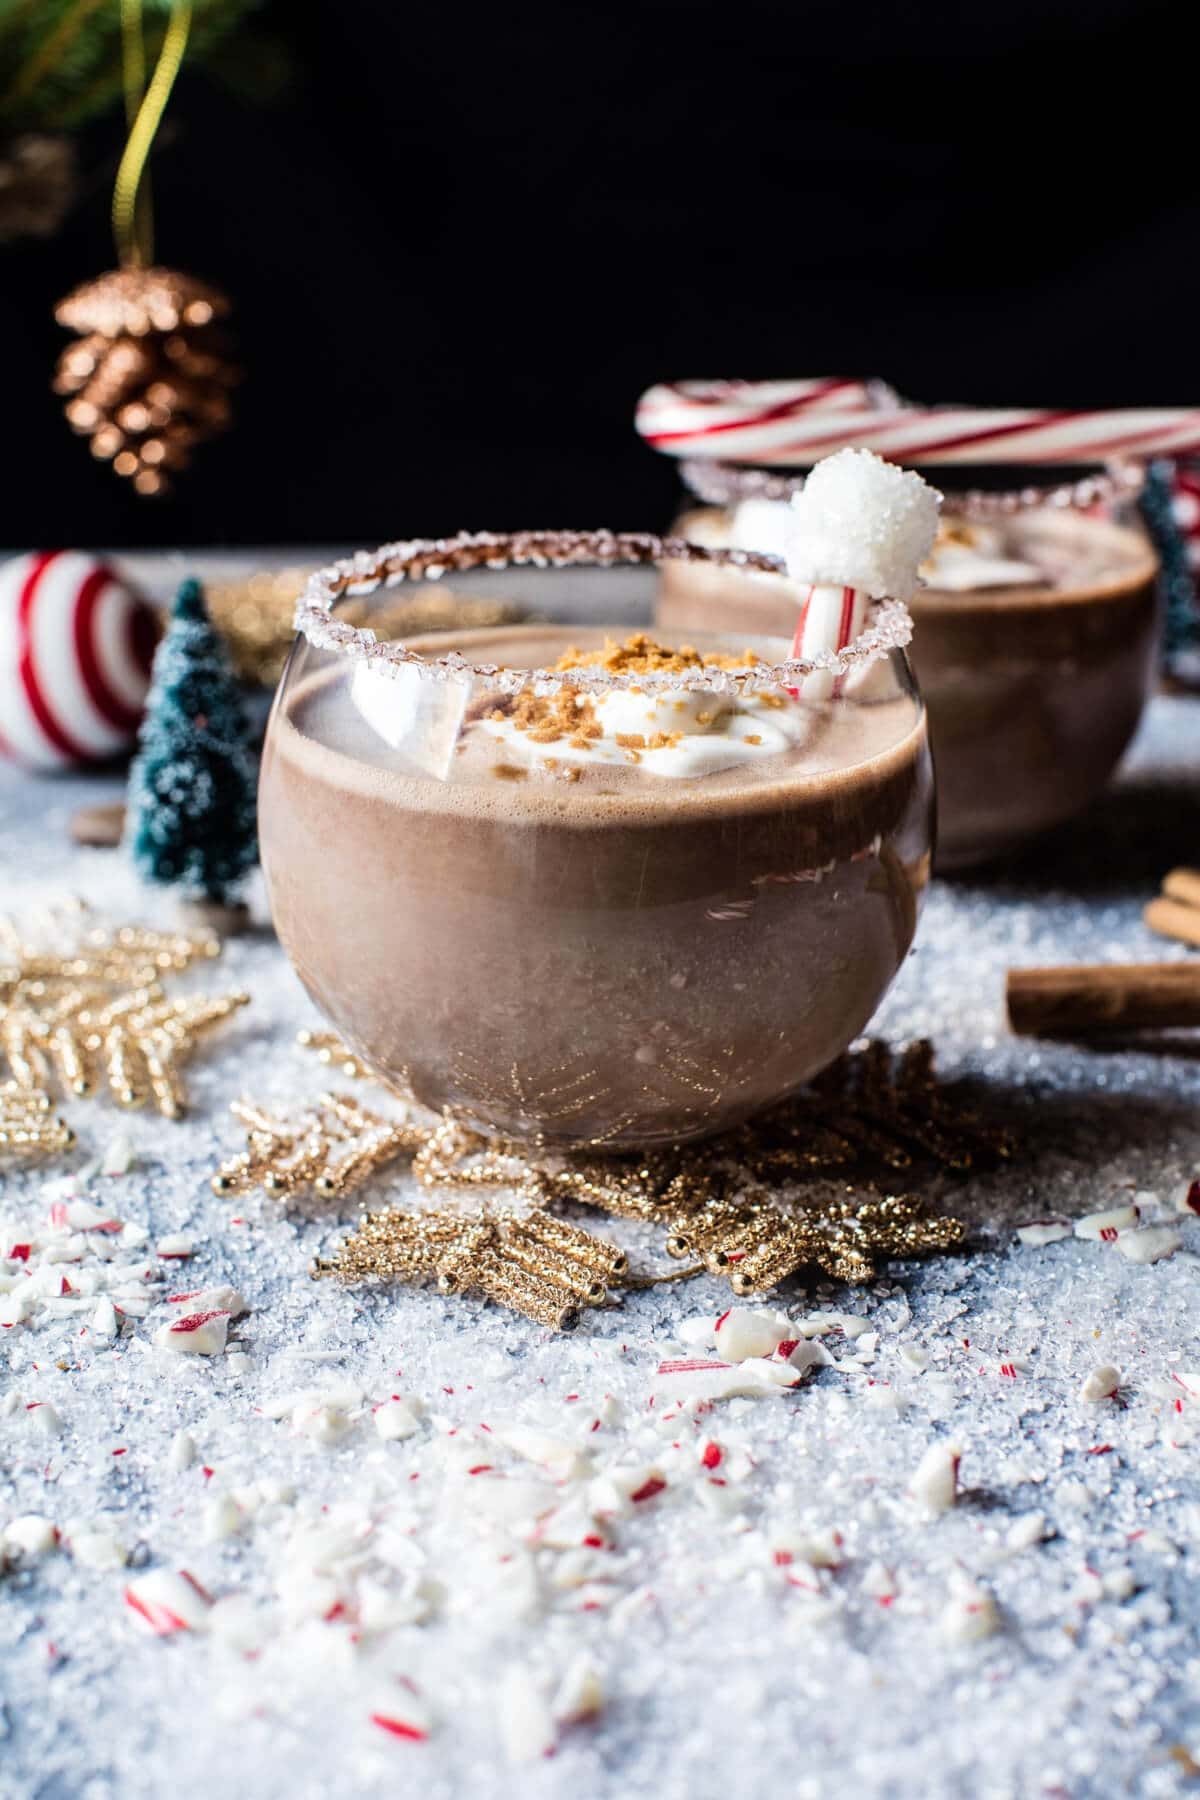
\includegraphics[width=1\textwidth,height=\textheight]{images/the-north-pole-.jpg}

\textbf{Prep Time:} 15 min \textbar{} \textbf{Cook Time:} \textbar{}
\textbf{Total Time:} 15 min

\section{Ingredients}\label{ingredients-167}

\begin{itemize}
\tightlist
\item
  4 ounces vodka
\item
  2 ounces Kahlúa (or more to taste)
\item
  4 tablespoons chocolate syrup
\item
  1 teaspoon vanilla extract
\item
  3 teaspoons molasses
\item
  1/8 teaspoon ginger
\item
  1/2 cup heavy cream or whole milk
\item
  whipped cream (candy canes and gingerbread cookies, for serving
  (optional))
\end{itemize}

\section{Instructions}\label{instructions-167}

\begin{enumerate}
\def\labelenumi{\arabic{enumi}.}
\tightlist
\item
\end{enumerate}

\bookmarksetup{startatroot}

\chapter{Crispy Belgian Waffles.}\label{crispy-belgian-waffles.}

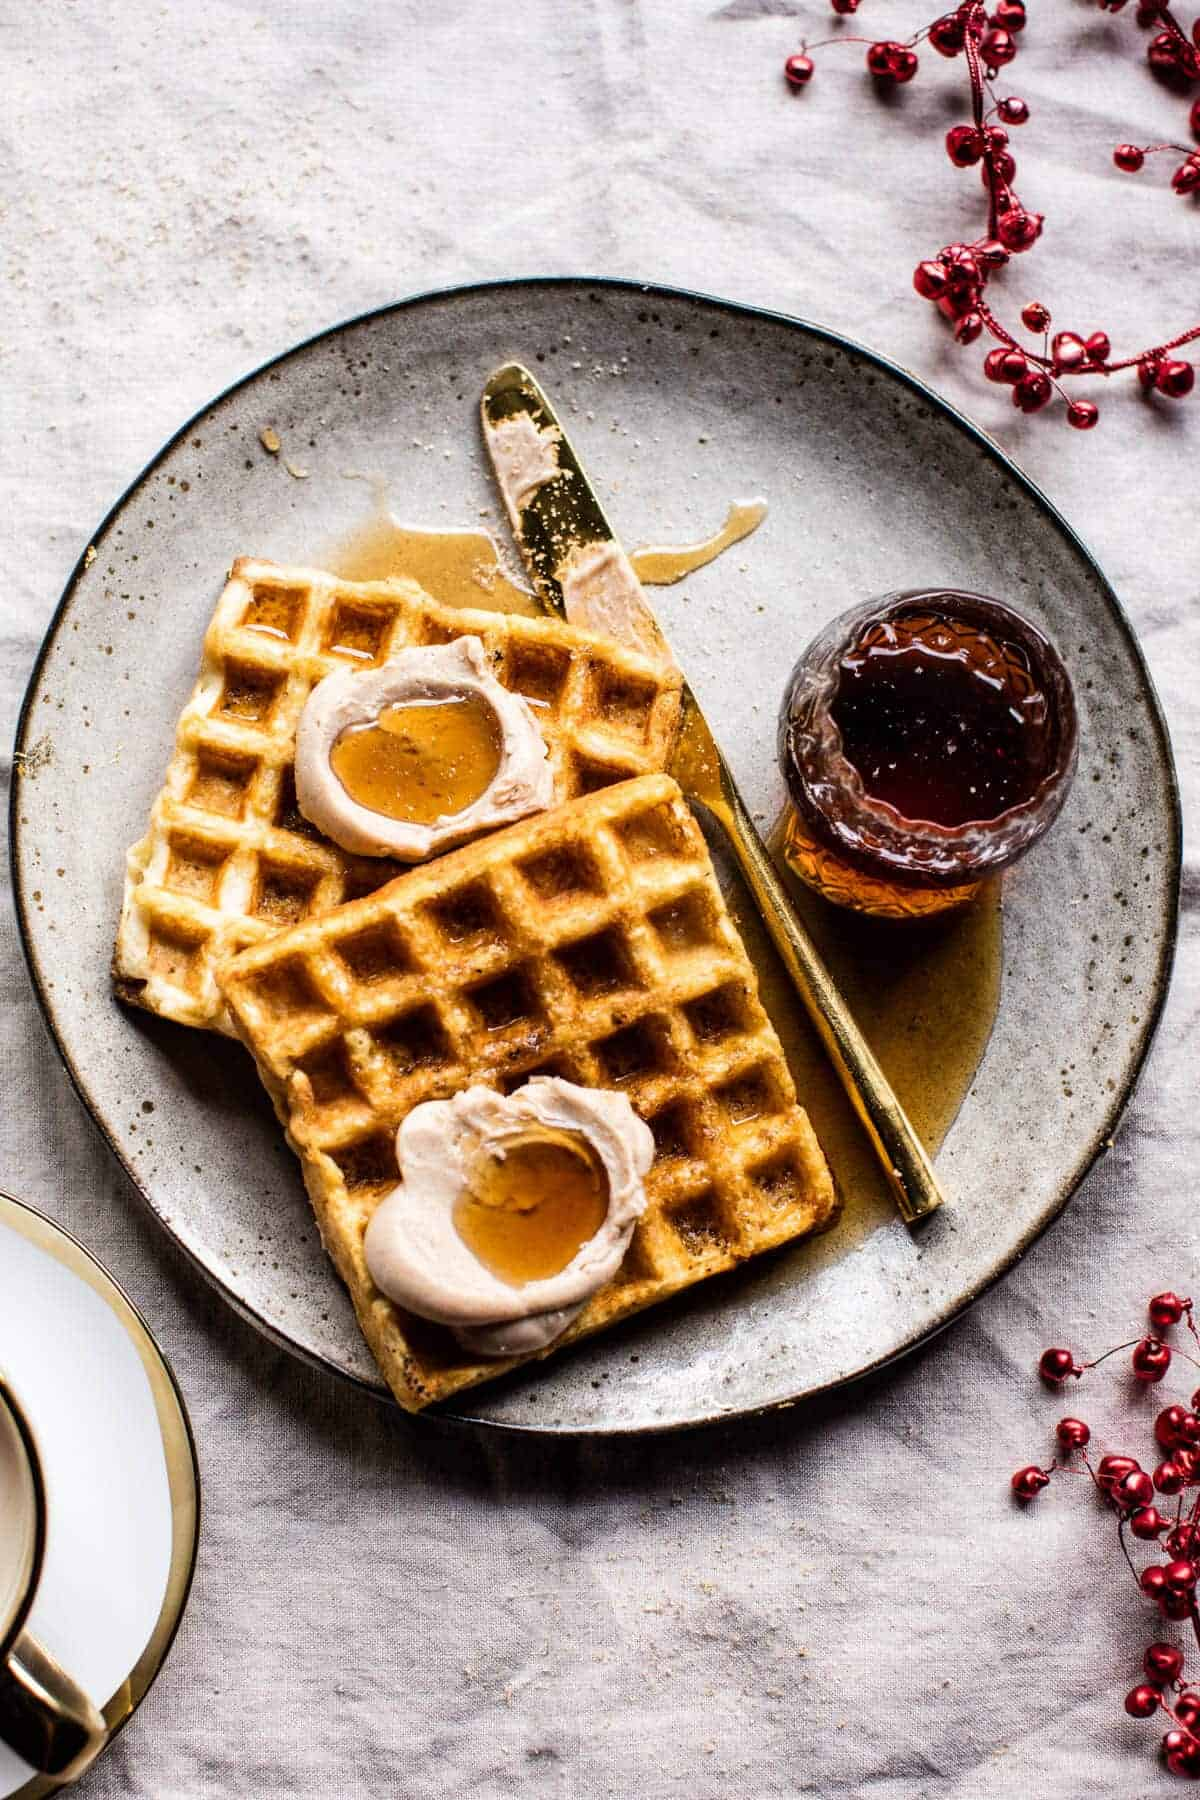
\includegraphics[width=1\textwidth,height=\textheight]{images/crispy-belgian-waffles-.jpg}

\textbf{Prep Time:} 15 min \textbar{} \textbf{Cook Time:} 5 min
\textbar{} \textbf{Total Time:} 20 min

\section{Ingredients}\label{ingredients-168}

\begin{itemize}
\tightlist
\item
  3/4 cup all-purpose flour
\item
  1/4 cup cornstarch
\item
  1/2 teaspoon salt
\item
  1/2 teaspoon baking powder
\item
  1/2 teaspoon baking soda
\item
  3/4 cup shaken buttermilk
\item
  1/4 cup water
\item
  1 large egg (separated)
\item
  6 tablespoons unsalted butter (melted and cooled)
\item
  1 teaspoon vanilla extract
\item
  3 tablespoons granulated sugar
\item
  whipped cream and fresh fruit (for serving)
\item
  8 tablespoon butter (softened)
\item
  2 tablespoons maple syrup
\item
  1/2 teaspoon cinnamon
\item
  1/4 teaspoon nutmeg
\item
  1/8 teaspoon cloves
\end{itemize}

\section{Instructions}\label{instructions-168}

\begin{enumerate}
\def\labelenumi{\arabic{enumi}.}
\tightlist
\item
  In a large bowl, whisk together the flour, cornstarch, salt, baking
  powder, and baking soda.
\item
  In a large measuring cup, whisk together the buttermilk, water, egg
  yolk, butter, and vanilla. Pour into the flour mixture and stir until
  just combined. Set aside.
\item
  In another bowl, with an electric mixer on high speed, beat the egg
  white until foamy. Add the sugar and beat until stiff, glossy peaks
  form. Fold into the reserved batter until just combined.
\item
  Cook the batter according to your waffle iron's instructions.
\item
  Top with the whipped eggnog butter, maple syrup, and fruit (if using).
\end{enumerate}

\bookmarksetup{startatroot}

\chapter{Thanksgiving Turkey Hot
Dish.}\label{thanksgiving-turkey-hot-dish.}

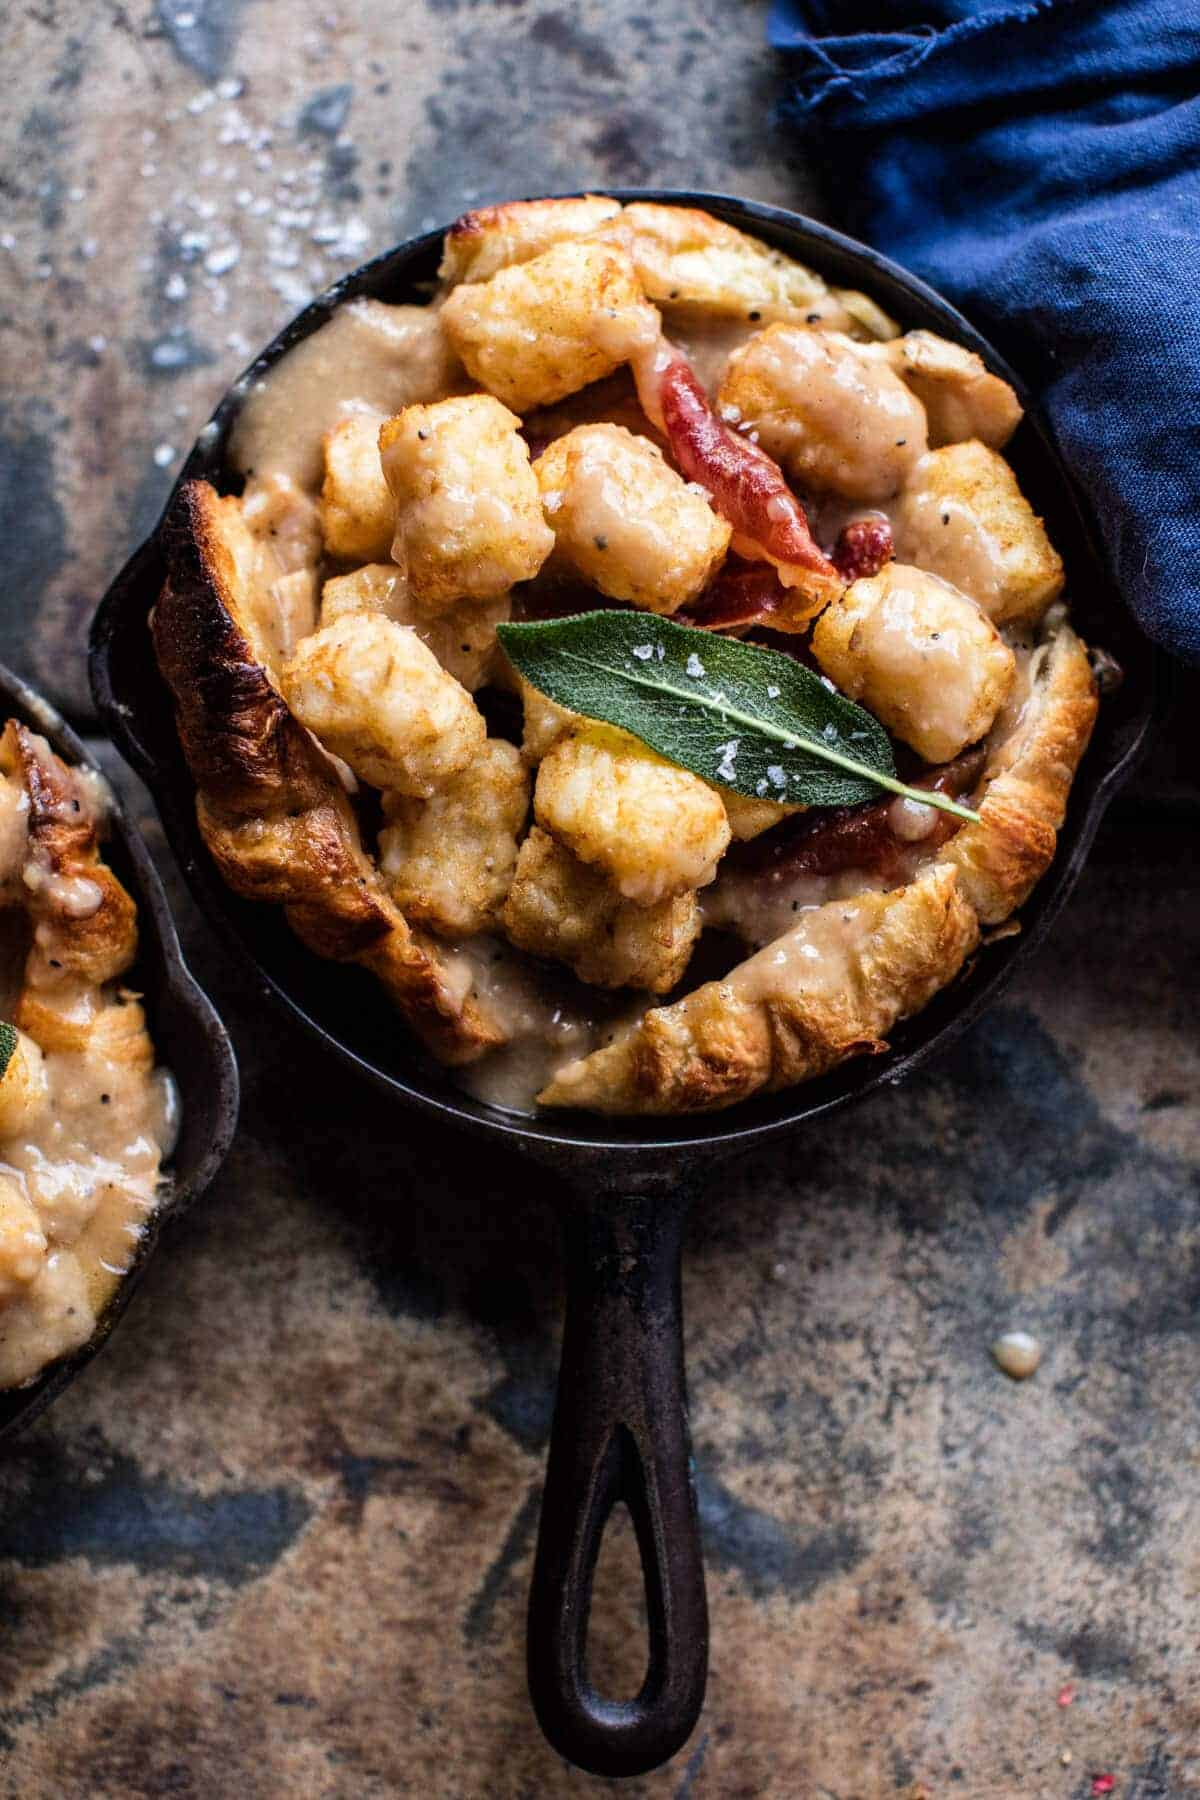
\includegraphics[width=1\textwidth,height=\textheight]{images/thanksgiving-turkey-hot-dish-.jpg}

\textbf{Prep Time:} 10 min \textbar{} \textbf{Cook Time:} 30 min
\textbar{} \textbf{Total Time:} 40 min

\section{Ingredients}\label{ingredients-169}

\begin{itemize}
\tightlist
\item
  4 croissants (halved)
\item
  4 tablespoons butter
\item
  cup leftover turkey (warmed (at least 1 ))
\item
  cup leftover gravy (warmed (at least 1 ))
\item
  1 1/2 cups shredded sharp cheddar cheese
\item
  3 ounces prosciutto (torn (optional))
\item
  2 cups tater tots
\item
  leftover cranberry sauce
\item
  fried sage (for serving)
\end{itemize}

\section{Instructions}\label{instructions-169}

\begin{enumerate}
\def\labelenumi{\arabic{enumi}.}
\tightlist
\item
  Preheat the oven to 375 degrees F. Grease a square baking dish or 10
  inch skillet.
\item
  Line the croissants, cut side up, in the baking dish and place a small
  pat of butter on each. Add the turkey in an even layer and then
  drizzle the gravy overtop. Top with a layer of cheese and then add the
  prosciutto. Arrange the tater tots in an even layer. Transfer to the
  oven and bake for 30-40 minutes or until the tater tots are crisp.
  Serve!
\end{enumerate}

\bookmarksetup{startatroot}

\chapter{Buttery Parker House Rolls.}\label{buttery-parker-house-rolls.}

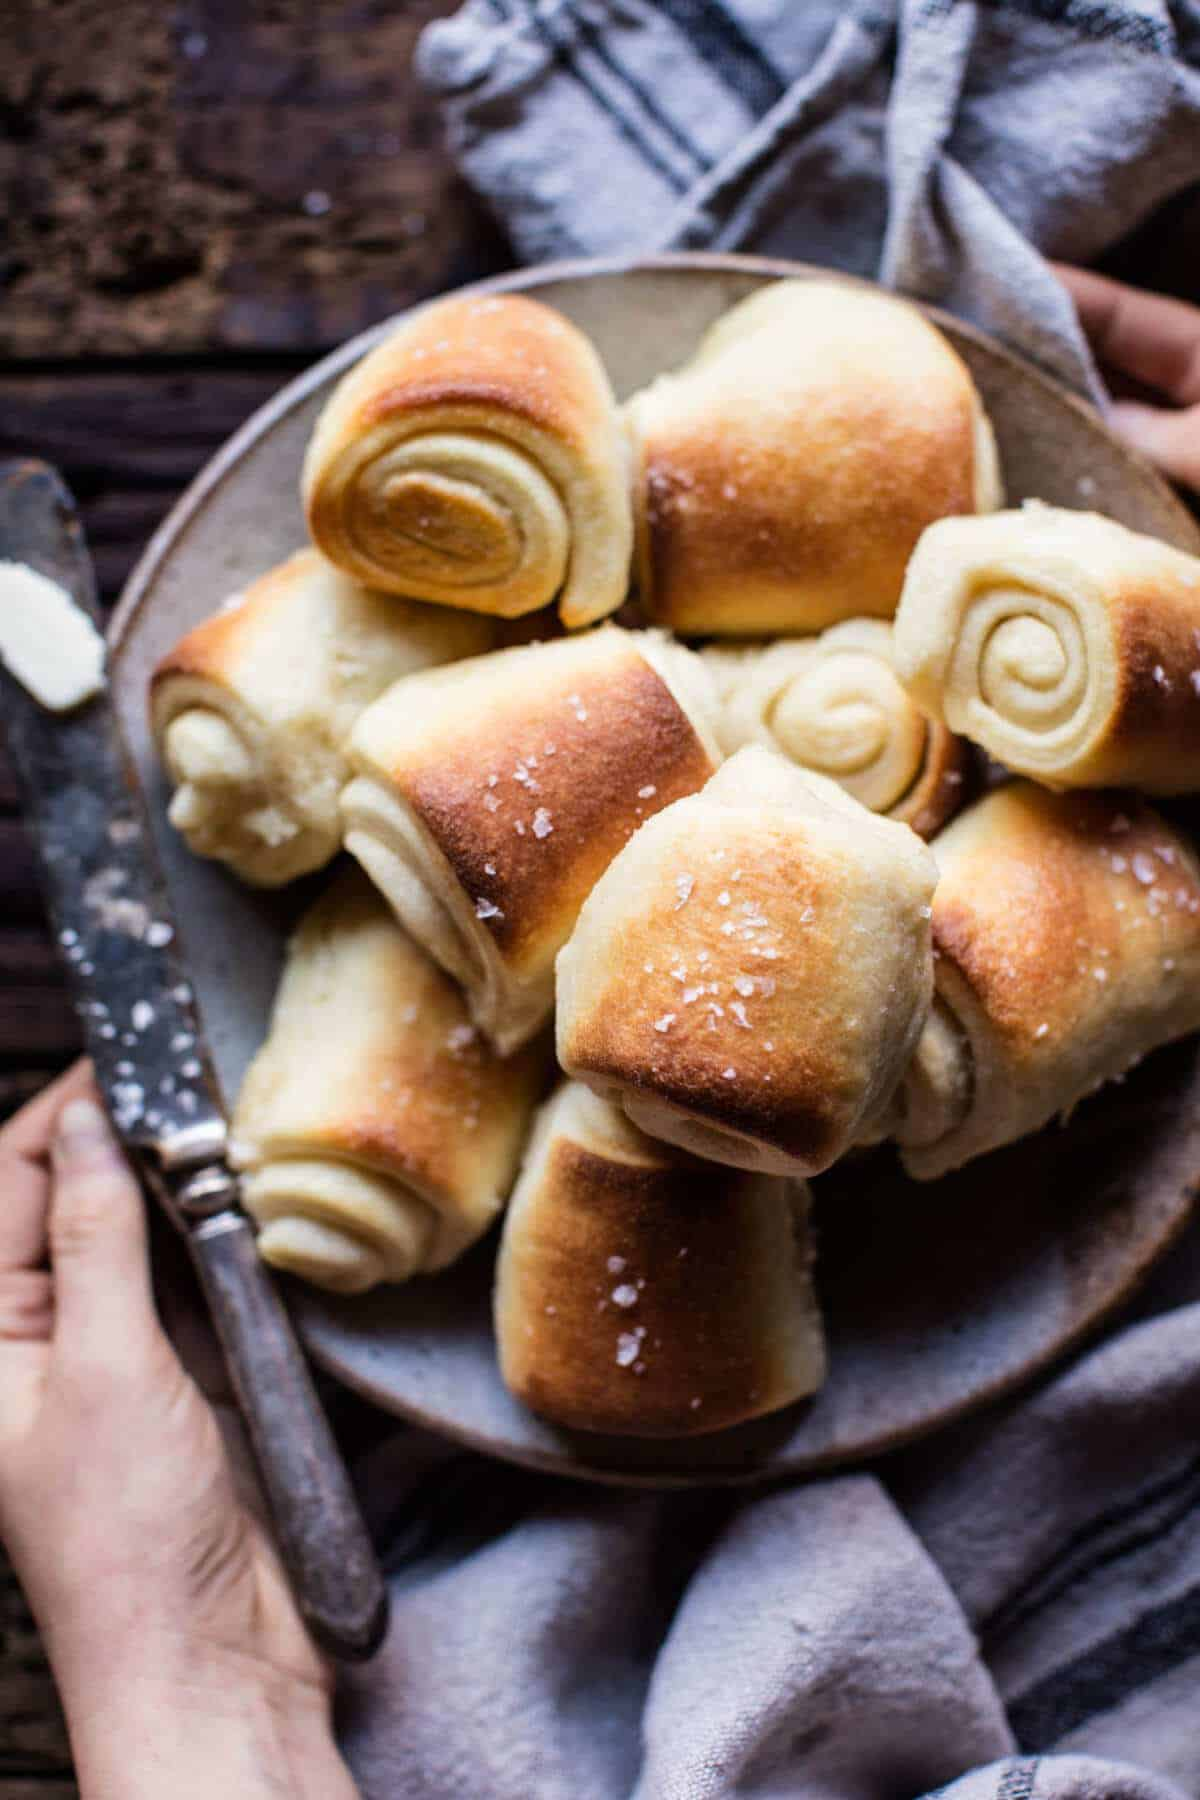
\includegraphics[width=1\textwidth,height=\textheight]{images/buttery-parker-house-rolls-.jpg}

\textbf{Prep Time:} \textbar{} \textbf{Cook Time:} 20 min \textbar{}
\textbf{Total Time:} 3 hr 10 min

\section{Ingredients}\label{ingredients-170}

\begin{itemize}
\tightlist
\item
  3 cups King Arthur Unbleached All-Purpose Flour
\item
  2 1/2 teaspoons instant yeast
\item
  3 tablespoons sugar
\item
  1 1/4 teaspoons salt
\item
  1/4 cup potato flour
\item
  3 tablespoons butter
\item
  1 cup milk
\item
  1 large egg
\item
  3 1/2 tablespoons to 4 butter, melted; for brushing on rolls
\end{itemize}

\section{Instructions}\label{instructions-170}

\begin{enumerate}
\def\labelenumi{\arabic{enumi}.}
\tightlist
\item
  In a large mixing bowl, or in the bowl of an electric mixer, combine
  all of the ingredients (except the 3 tablespoons melted butter at the
  end), mixing to form a shaggy dough. Note: to speed the rising
  process, whisk together the milk and egg, and heat gently just enough
  to remove the refrigerator chill; then add to the remaining
  ingredients.
\item
  Knead the dough, by hand (10 minutes) or by machine (7 to 8 minutes)
  until it's smooth.
\item
  Place the dough in a lightly greased bowl or 8-cup measure (so you can
  track its rising progress). Allow it to rise for 90 minutes; it'll
  become quite puffy, though it probably won't double in bulk. Note that
  the dough takes quite awhile to get going; after 1 hour, it may seem
  like it's barely expanded at all. But during the last half hour, it
  rises more quickly.
\item
  Transfer the dough to a lightly greased work surface. Divide it in
  half. Working with one half at a time, roll or pat the dough into an
  8'' x 12'' rectangle.
\item
  Brush the dough all over with a light coating of the melted butter.
  You'll have melted butter left over; save it to brush on top of the
  baked rolls.
\item
  Cut the dough in half lengthwise, to make two 4'' x 12'' rectangles.
  Working with one rectangle at a time, fold it lengthwise to about
  1/2'' of the other edge, so the bottom edge sticks out about 1/2''
  beyond the top edge. You'll now have a rectangle that's about 2 1/4''
  x 12''. Repeat with the other piece of dough.
\item
  Cut each of the rectangles crosswise into four 3'' pieces, making a
  total of 8 rolls, each about 2 1/4'' x 3''. Place the rolls, smooth
  side up, in a lightly greased 9'' x 13'' pan. Repeat with the
  remaining piece of dough, making 16 rolls in all. Alternately you can
  roll each rectangle of dough into a coil as you would a cinnamon roll.
\item
  You'll arrange 4 rows of 4 in the pan, with the longer side of the
  rolls going down the longer side of the pan. Gently flatten the rolls
  to pretty much cover the bottom of the pan.
\item
  Cover the pan, and let the rolls rise for about 45 minutes to 1 hour,
  until they're puffy but definitely not doubled. Towards the end of the
  rising time, preheat the oven to 350°F.
\item
  Bake the rolls for 20 to 25 minutes, until they're golden brown and
  feel set.
\item
  Remove them from the oven, and brush with the remaining melted butter.
  Pull them apart to serve.
\end{enumerate}

\bookmarksetup{startatroot}

\chapter{Turkey Enchilada Quinoa
Soup.}\label{turkey-enchilada-quinoa-soup.}

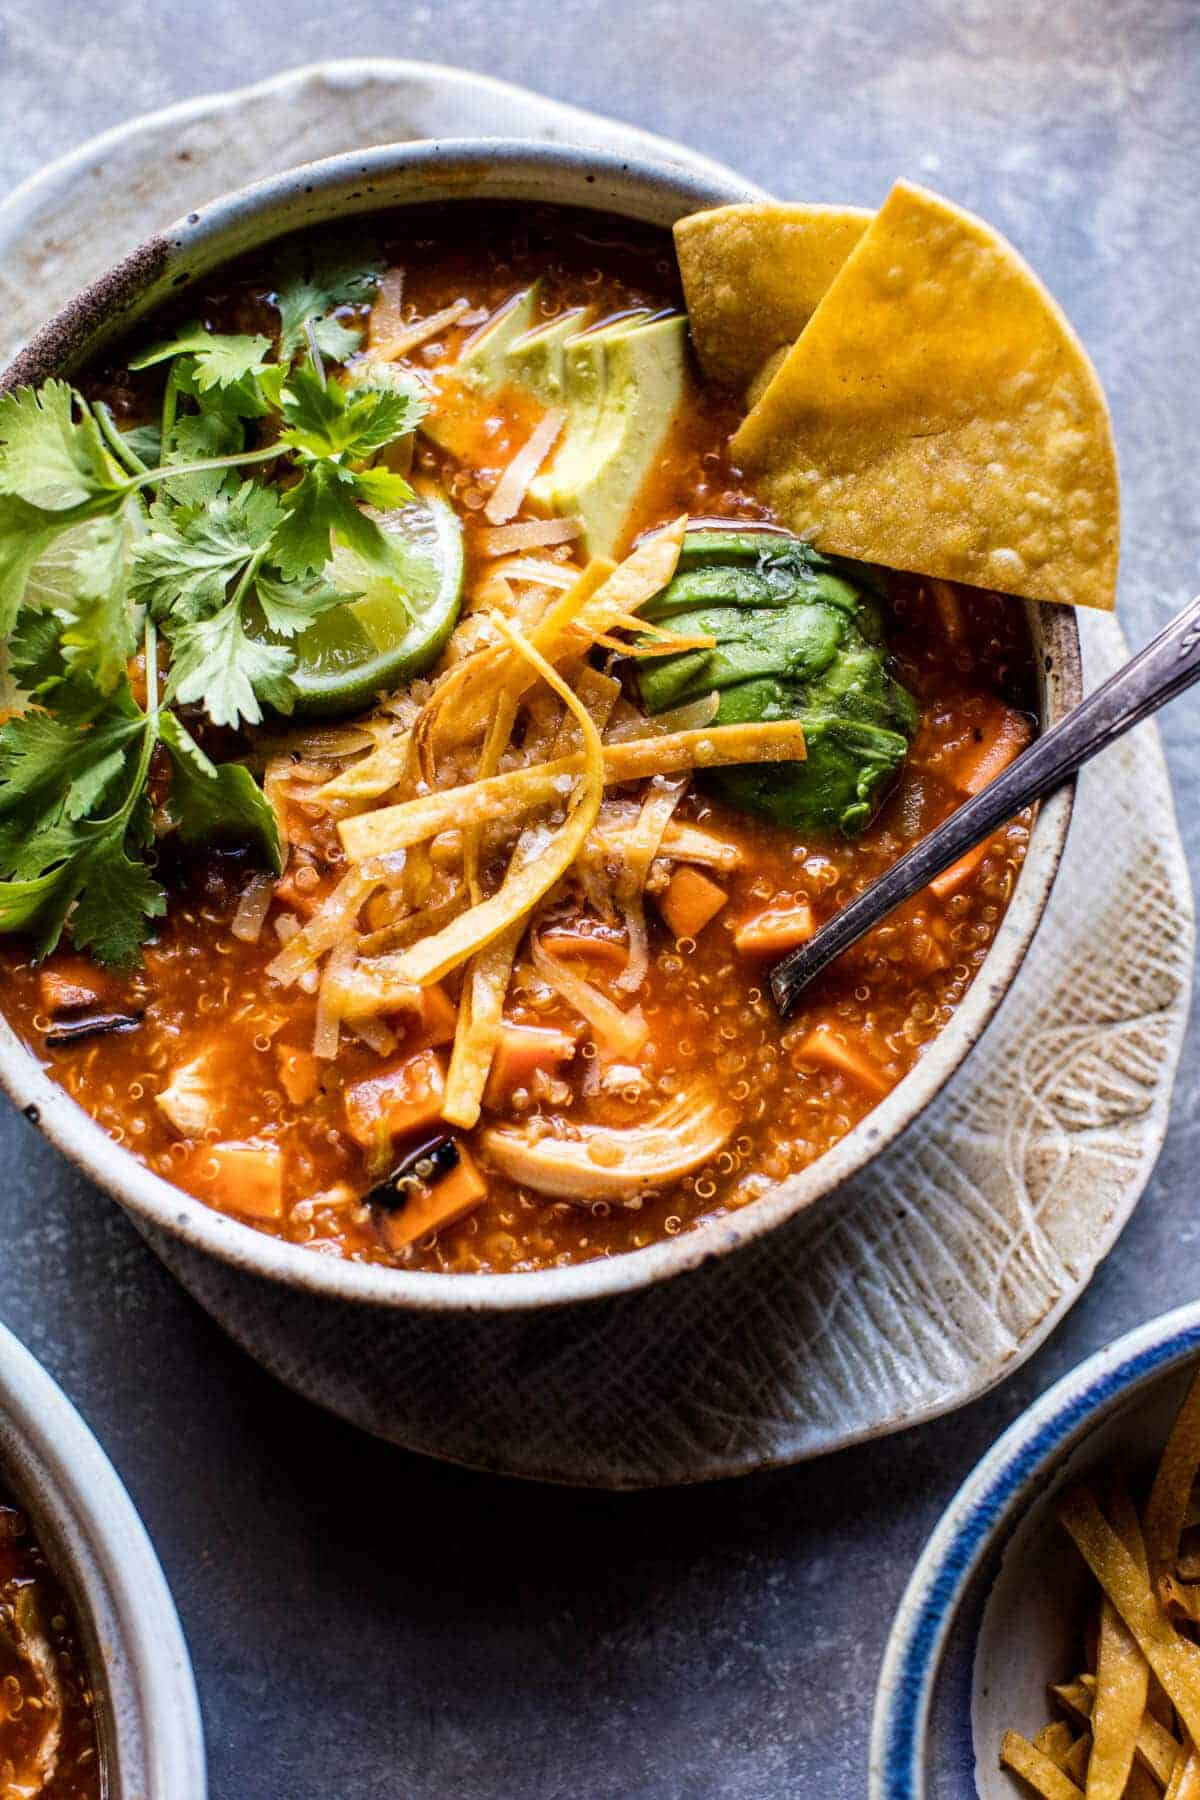
\includegraphics[width=1\textwidth,height=\textheight]{images/turkey-enchilada-quinoa-soup-.jpg}

\textbf{Prep Time:} 10 min \textbar{} \textbf{Cook Time:} 20 min
\textbar{} \textbf{Total Time:} 30 min

\section{Ingredients}\label{ingredients-171}

\begin{itemize}
\tightlist
\item
  2 tablespoons olive oil
\item
  1 small sweet onion
\item
  1 sweet potato (chopped (peel if you’d like))
\item
  3 cups low sodium chicken broth (plus more if needed)
\item
  3 ounce cans Old El Paso Enchilada Sauce (10)
\item
  1 ounce can Old El Paso Chopped Green Chiles (4)
\item
  ½ cup dry quinoa
\item
  1-2 cups shredded turkey (may also use shredded chicken)
\item
  1 ounce can black beans (drained and rinsed, 14)
\item
  1-2 cups shredded cheddar cheese
\item
  diced avocado (cilantro, and tortilla crisp/chips, for serving)
\end{itemize}

\section{Instructions}\label{instructions-171}

\begin{enumerate}
\def\labelenumi{\arabic{enumi}.}
\tightlist
\item
  Heat the oil in a large stockpot over medium-high heat. When the oil
  shimmers, add the onion and sweet potatoes. Season with salt and
  pepper and cook for 5-8 minutes or until softened and the onion
  fragrant. Slowly pour in the chicken broth, enchilada sauce, green
  chiles, and 1 cup water. Bring the mix to a boil over high heat. Add
  the quinoa, cover and reduce the heat to low. Cook for 15 minutes or
  until the quinoa is soft. Stir in the turkey, black beans, and 1 cup
  cheddar cheese. Cook until the cheese is melted and the turkey warm,
  about 5 minutes. Remove from the heat.
\item
  Ladle the soup into bowls, garnish with avocado, cheddar cheese,
  cilantro and chips. Eat!
\end{enumerate}

\bookmarksetup{startatroot}

\chapter{Butter Pecan Frosted Fudge
Brownies.}\label{butter-pecan-frosted-fudge-brownies.}

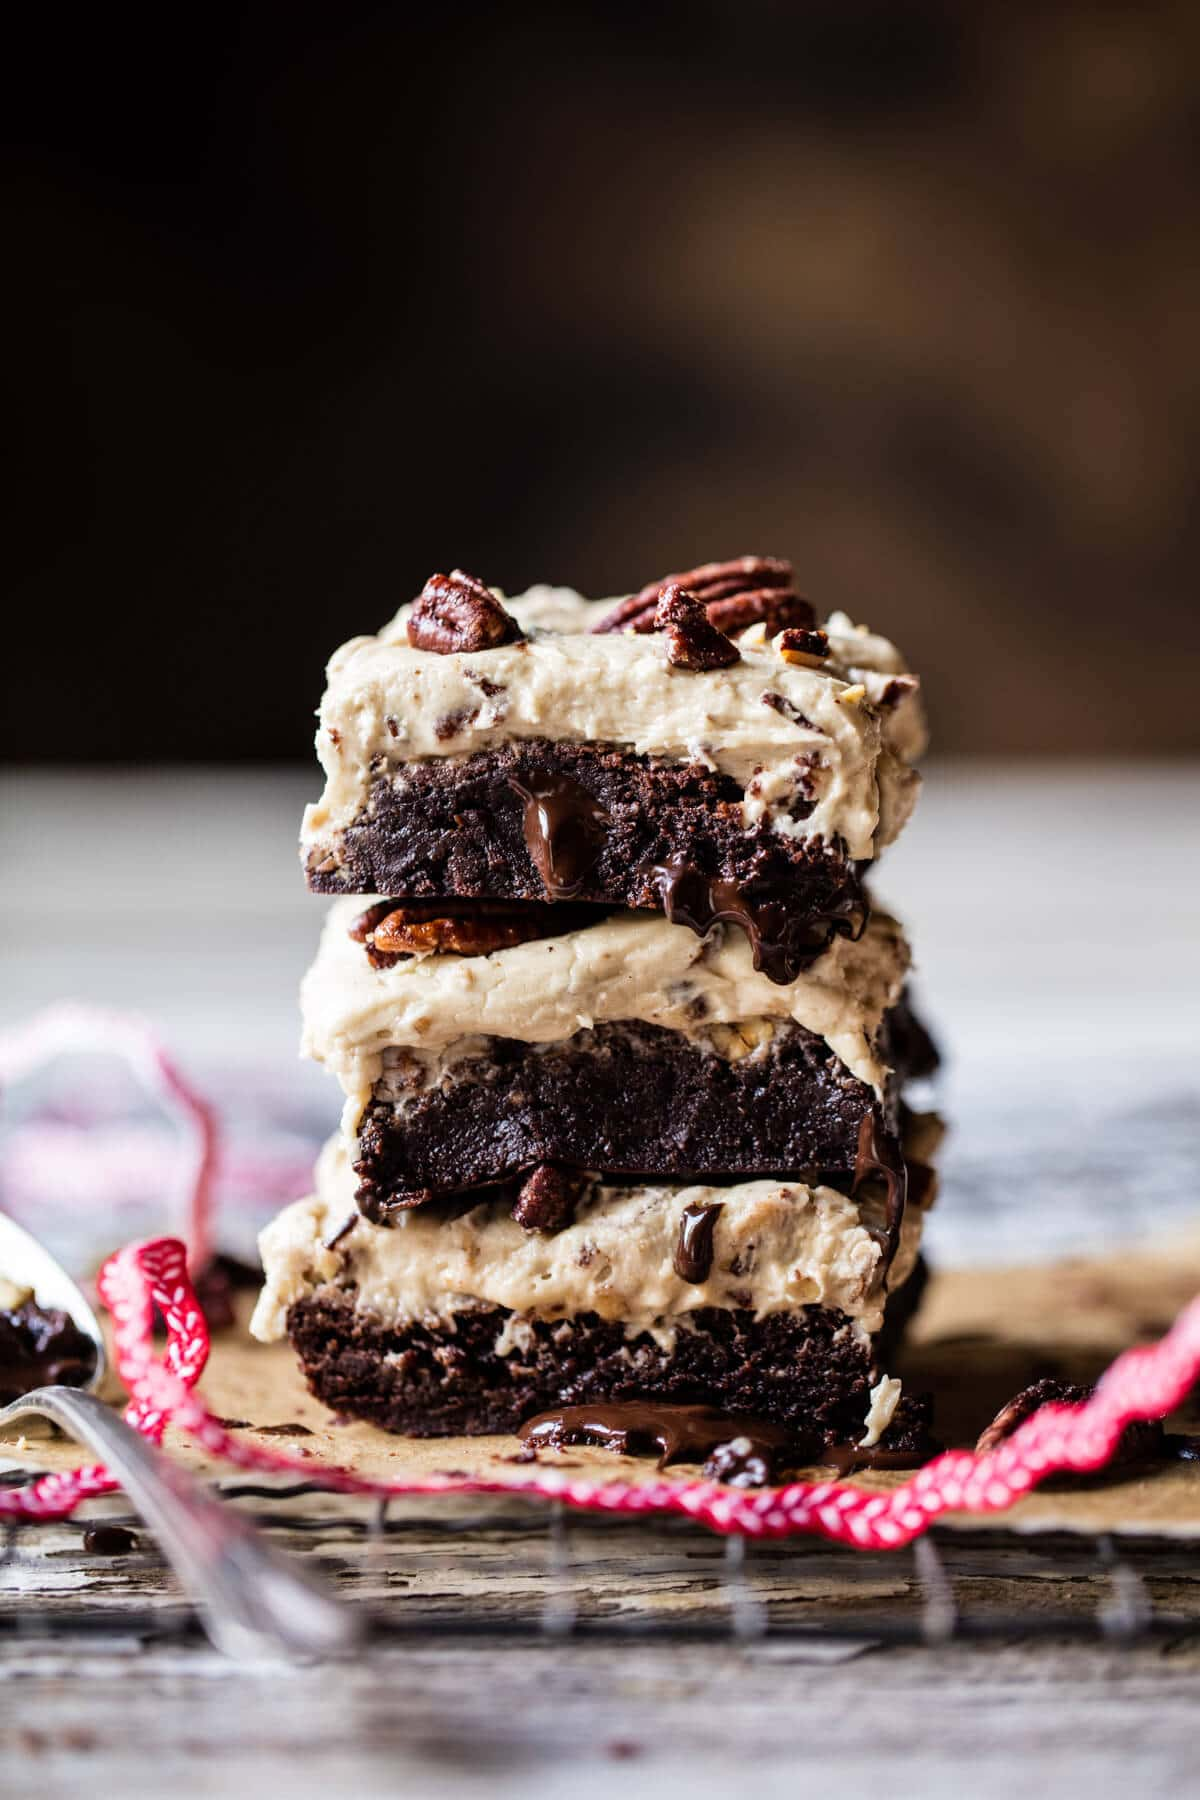
\includegraphics[width=1\textwidth,height=\textheight]{images/butter-pecan-frosted-fudge-brownies-.jpg}

\textbf{Prep Time:} 30 min \textbar{} \textbf{Cook Time:} 30 min
\textbar{} \textbf{Total Time:} 1 hr

\section{Ingredients}\label{ingredients-172}

\begin{itemize}
\tightlist
\item
  2 sticks (1 cup) unsalted butter
\item
  4 ounces milk or dark chocolate, chopped
\item
  1 1/2 cups granulated sugar
\item
  1 tablespoon vanilla extract
\item
  4 large eggs
\item
  1 cup unsweetened cocoa powder
\item
  1 cup all-purpose flour
\item
  1/4 teaspoon kosher salt
\item
  1/2 cup chopped milk or dark chocolate
\item
  1 1/2 sticks (12 tablespoons) unsalted butter
\item
  2/3 cup heavy cream
\item
  1 cup plus 2 tablespoons packed brown sugar
\item
  1 1/2 cups raw pecans
\item
  2 tablespoons bourbon (optional)
\item
  3 teaspoons vanilla extract
\item
  1/4 teaspoon cinnamon
\item
  3 cups powdered sugar
\end{itemize}

\section{Instructions}\label{instructions-172}

\begin{enumerate}
\def\labelenumi{\arabic{enumi}.}
\tightlist
\item
  Preheat the oven to 350 degrees F. Line a 9x13 inch baking dish with
  parchment paper.
\item
  Add the butter and chocolate to a medium microwave safe mixing bowl.
  Microwave on 30 second intervals, stirring after each interval, until
  melted and smooth. To the melted chocolate whisk in the sugar, vanilla
  and eggs and until smooth. Stir in the cocoa powder, flour and salt
  until just combined, try not to over mix the batter. It will be thick.
  Stir in chopped chocolate. Pour the batter into the prepared pan,
  spreading it in an even layer. Transfer to the oven and bake for 25-30
  minutes, until the brownies are set on top. Remove from the oven and
  allow to cool.
\item
  Meanwhile, make the frosting. Preheat oven to 350 degrees F.
\item
  In a medium sauce pan, melt together 4 tablespoons butter, the cream,
  and brown sugar. Bring to a boil and cook for one minute or until the
  sugar is dissolved. Remove from the heat and add to the bowl of a
  stand mixer. Place the bowl in the freezer (or fridge for longer) for
  15-20 minutes or until cool to touch.
\item
  On a parchment lined baking sheet, combine the pecans, bourbon - if
  using, 1 teaspoon vanilla, the remaining 2 tablespoons brown sugar and
  cinnamon and toss to coat. Transfer to the oven and bake for 10 to 15
  minutes, stirring occasionally, until toasted. Remove, let cool 10
  minutes, then roughly chop the pecans.
\item
  Grab the cooled butter mixture from the freezer and add the remaining
  8 tablespoons butter, remaining 2 teaspoons vanilla and powdered sugar
  to the bowl and beat together until well combined. Fold in half of the
  chopped pecans. Spread the frosting onto the cooled brownies. Top with
  remaining pecans, using as many as desired. Slice and serve or store
  in and airtight container.
\end{enumerate}

\bookmarksetup{startatroot}

\chapter{Cranberry Roasted Butternut Persimmon Salad with Fried Goat
Cheese.}\label{cranberry-roasted-butternut-persimmon-salad-with-fried-goat-cheese.}

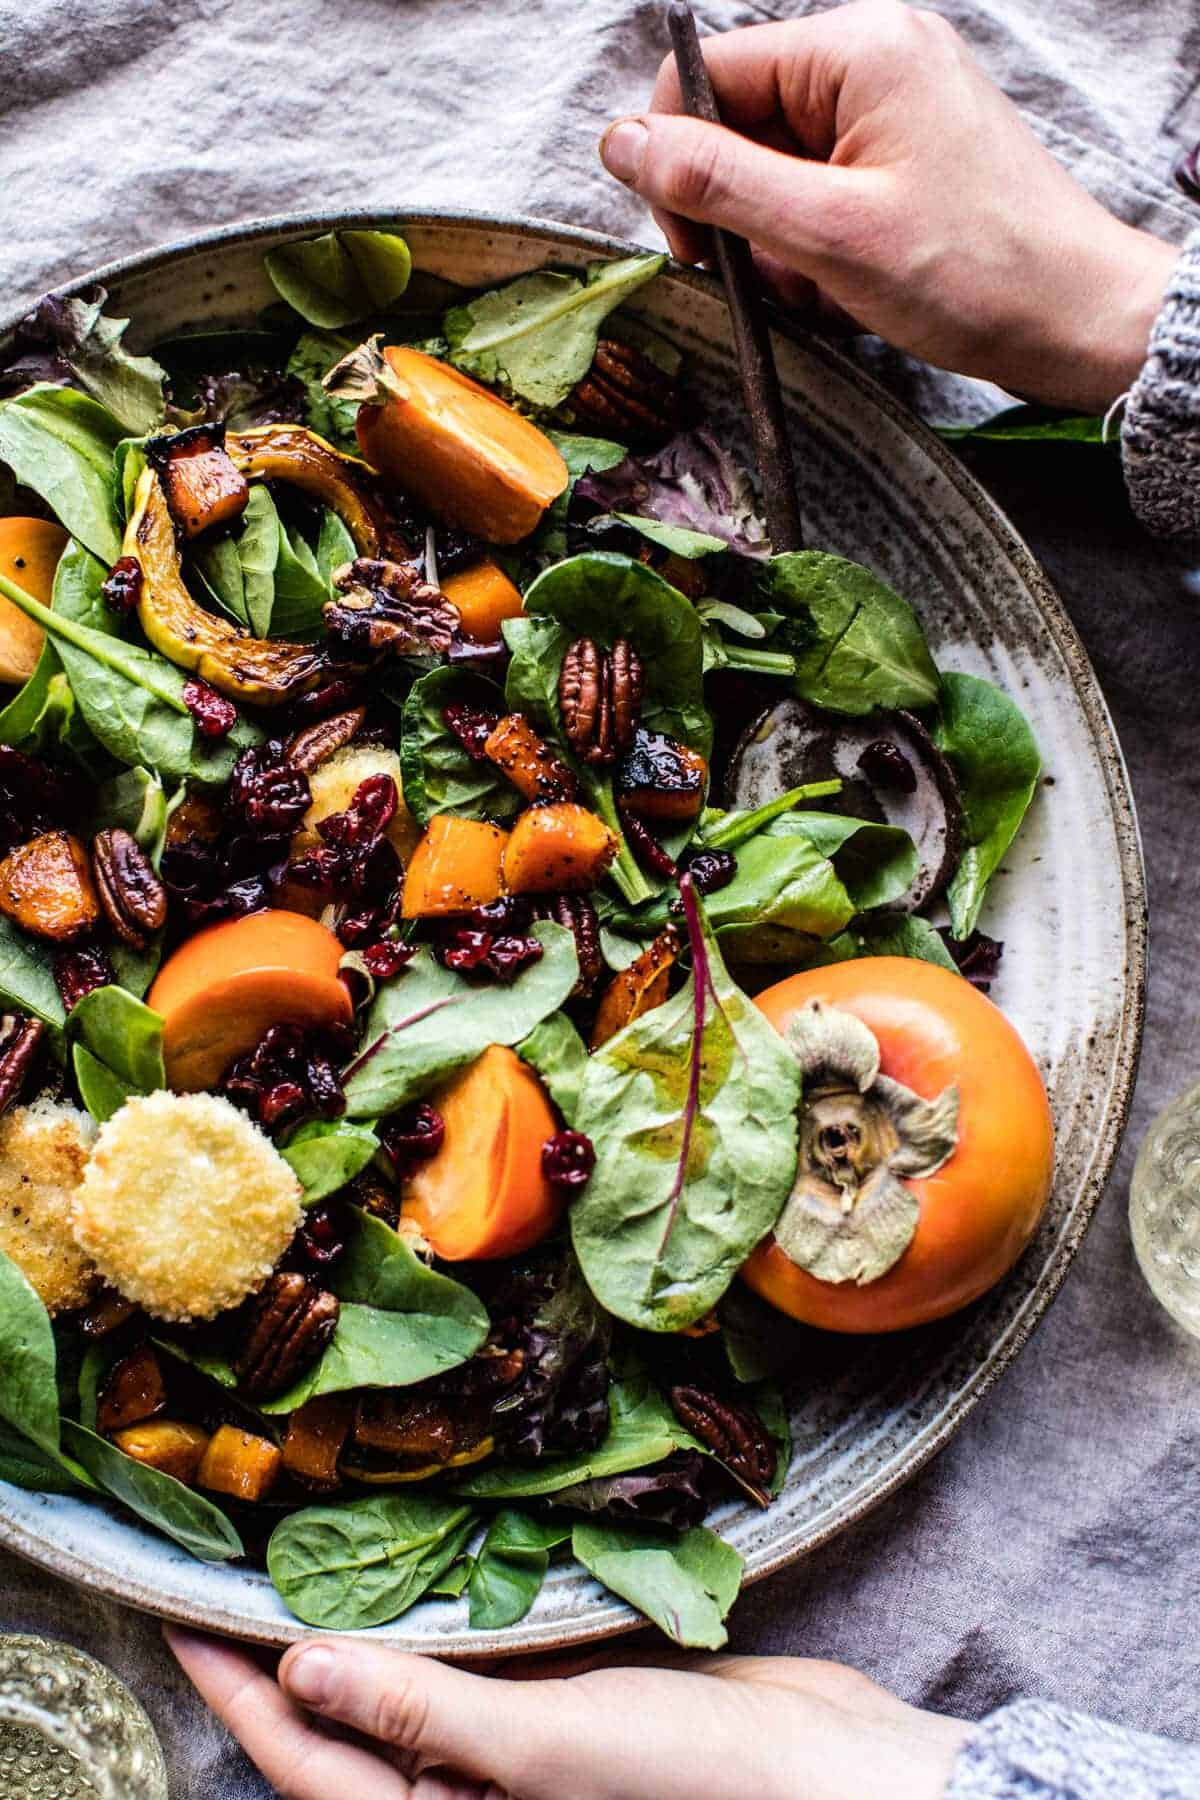
\includegraphics[width=1\textwidth,height=\textheight]{images/cranberry-roasted-butternut-persimmon-salad-with-fried-goat-cheese-.jpg}

\textbf{Prep Time:} 15 min \textbar{} \textbf{Cook Time:} 30 min
\textbar{} \textbf{Total Time:} 45 min

\section{Ingredients}\label{ingredients-173}

\begin{itemize}
\tightlist
\item
  4 cups cubed butternut squash (or a mix of butternut and delicata)
\item
  1/2 cup plus 2 tablespoons olive oil
\item
  2 tablespoons maple syrup
\item
  1/2 teaspoon cinnamon
\item
  1/4 teaspoon ginger
\item
  1/4 teaspoon cayenne
\item
  kosher salt and pepper
\item
  1/2 cup dried cranberries
\item
  3/4 cup apple cider
\item
  2 tablespoons apple cider vinegar
\item
  2 teaspoons dijon mustard
\item
  1 ounce log cut cheese (sliced into 1/4 inch rounds, 10)
\item
  1/3 cup buttermilk (or 1 egg beaten)
\item
  1/3 cup panka bread crumbs
\item
  6 cups mixed greens
\item
  3 persimmons (quartered)
\item
  1/2 cup toasted pecans
\end{itemize}

\section{Instructions}\label{instructions-173}

\begin{enumerate}
\def\labelenumi{\arabic{enumi}.}
\tightlist
\item
  Preheat the oven to 425 degrees F.
\item
  Spread the butternut squash out in a single layer on a baking sheet.
  Drizzle 2 tablespoons olive oil, maple syrup, cinnamon, ginger,
  cayenne, salt and pepper, toss well to coat. Roast in the oven until
  the butternut squash is tender, 20 to 25 minutes, stirring halfway
  through cooking. Remove from oven and stir in cranberries.
\item
  Meanwhile, heat the apple cider and the cider vinegar in a small
  saucepan over high heat and boil until it has reduced to 1/4 cup,
  about 6-8 minutes. Remove from the heat and whisk in the remaining 1/2
  cup olive oil and the mustard. Season with salt and pepper.
\item
  To make the Fried Goat Cheese. Heat 2 tablespoons olive oil in a
  skillet over medium heat.
\item
  Add the panko to one small bowl, then add the buttermilk to another
  small bowl. Carefully dip the rounds of goat cheese, first through the
  buttermilk, and then dredge through the panko. Carefully add to the
  hot skillet and cook for 2-3 minutes per side or until golden. To make
  these in advance, fry as directed and then warm in a 300 degree oven
  for 5 minutes.
\item
  In a large salad bowl, toss together the lettuce, roasted squash,
  persimmons, and pecans. Add the dressing and toss once more. Top with
  the fried goat cheese. Enjoy warm or at room temperature.
\end{enumerate}

\bookmarksetup{startatroot}

\chapter{Cream of Mushroom Chicken Wild Rice
Soup.}\label{cream-of-mushroom-chicken-wild-rice-soup.}

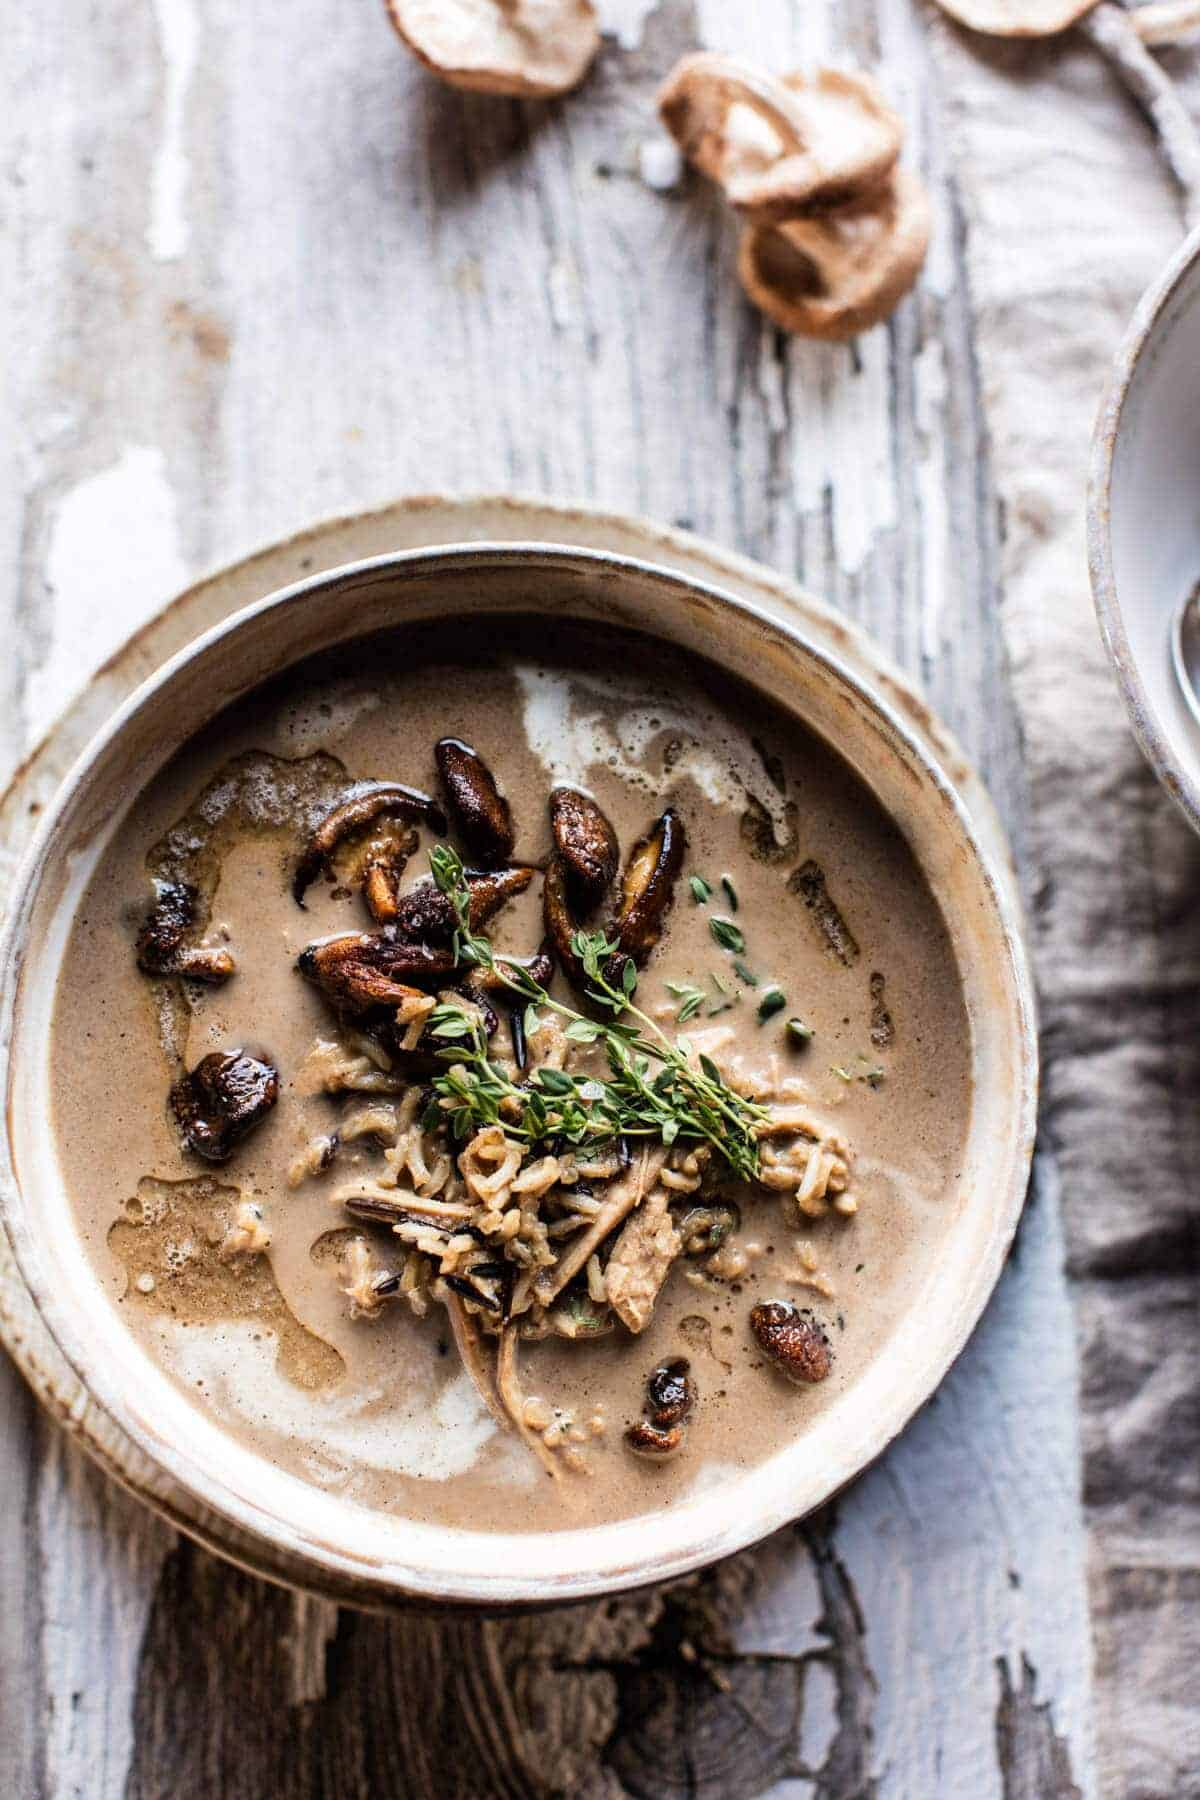
\includegraphics[width=1\textwidth,height=\textheight]{images/cream-of-mushroom-chicken-wild-rice-soup-.jpg}

\textbf{Prep Time:} 15 min \textbar{} \textbf{Cook Time:} 45 min
\textbar{} \textbf{Total Time:} 1 hr

\section{Ingredients}\label{ingredients-174}

\begin{itemize}
\tightlist
\item
  2 tablespoons butter
\item
  1 tablespoon olive oil
\item
  4 cloves garlic (smashed)
\item
  1/2 sweet onion (chopped)
\item
  kosher salt and pepper
\item
  6 ounces cremini mushrooms
\item
  2 ounces wild mushrooms
\item
  1 tablespoon fresh chopped thyme
\item
  6 cups low sodium chicken broth
\item
  1 cup wild rice
\item
  1/2-1 pound boneless (skinless chicken breasts or tenders)
\item
  1 cup whole milk
\item
  1/2 cup grated parmesan
\end{itemize}

\section{Instructions}\label{instructions-174}

\begin{enumerate}
\def\labelenumi{\arabic{enumi}.}
\tightlist
\item
  Melt the butter and olive oil in a large, heavy bottomed soup pot over
  medium heat. Add the garlic and onion and cook for 5-8 minutes,
  stirring often until the onion is soft. Season with salt and pepper.
  Add the cremini mushrooms and the wild mushrooms, cook another 5
  minutes or until the mushrooms are caramelized. Stir in the thyme and
  cook another minute longer. Remove the pot from the heat and ladle out
  half of the wild mushrooms. Transfer the remaining ingredients to a
  food processor. Add 2 cups broth and pulse until smooth, about 2
  minutes.
\item
  Return the mixture to the soup pot and add the remaining 4 cups broth
  plus 2 cups water. Bring the mixture to boil and stir in the rice and
  chicken. Cover and reduce the heat to medium low. Simmer for 30
  minutes or until the rice is tender and the chicken has cooked
  through. Shred the chicken in the pot. Stir in the milk and parmesan.
  Season the soup with salt + pepper. Simmer the soup for 5-10 minutes
  until warmed through.
\item
  Ladle the soup into bowls. Top with the reserved wild mushrooms (warm
  them if needed). Enjoy!
\end{enumerate}



\end{document}
